\documentclass[letterpaper]{book}
\usepackage{makeidx}
\usepackage{graphicx}
\usepackage{multicol}
\usepackage{float}
\usepackage{listings}
\usepackage{color}
\usepackage{textcomp}
\usepackage{alltt}
\usepackage{times}
\usepackage{ifpdf}
\ifpdf
\usepackage[pdftex,
            pagebackref=true,
            colorlinks=true,
            linkcolor=blue,
            unicode
           ]{hyperref}
\else
\usepackage[ps2pdf,
            pagebackref=true,
            colorlinks=true,
            linkcolor=blue,
            unicode
           ]{hyperref}
\usepackage{pspicture}
\fi
\usepackage[utf8]{inputenc}
\usepackage{doxygen}
\lstset{language=C++,inputencoding=utf8,basicstyle=\footnotesize,breaklines=true,breakatwhitespace=true,tabsize=8,numbers=left }
\makeindex
\setcounter{tocdepth}{3}
\renewcommand{\footrulewidth}{0.4pt}
\begin{document}
\hypersetup{pageanchor=false}
\begin{titlepage}
\vspace*{7cm}
\begin{center}
{\Large CIRIS \\[1ex]\large 1 }\\
\vspace*{1cm}
{\large Generated by Doxygen 1.6.1}\\
\vspace*{0.5cm}
{\small Thu Feb 9 12:52:30 2017}\\
\end{center}
\end{titlepage}
\clearemptydoublepage
\pagenumbering{roman}
\tableofcontents
\clearemptydoublepage
\pagenumbering{arabic}
\hypersetup{pageanchor=true}
\chapter{Modules Index}
\section{Modules List}
Here is a list of all modules with brief descriptions:\begin{DoxyCompactList}
\item\contentsline{section}{\hyperlink{namespacebranchmod}{branchmod} }{\pageref{namespacebranchmod}}{}
\item\contentsline{section}{\hyperlink{namespacebsimple}{bsimple} }{\pageref{namespacebsimple}}{}
\item\contentsline{section}{\hyperlink{namespacefunctiondefs}{functiondefs} }{\pageref{namespacefunctiondefs}}{}
\item\contentsline{section}{\hyperlink{namespacegp}{gp} }{\pageref{namespacegp}}{}
\item\contentsline{section}{\hyperlink{namespacemc__toolbox}{mc\_\-toolbox} }{\pageref{namespacemc__toolbox}}{}
\item\contentsline{section}{\hyperlink{namespacenewmod}{newmod} }{\pageref{namespacenewmod}}{}
\item\contentsline{section}{\hyperlink{namespaceparameters}{parameters} }{\pageref{namespaceparameters}}{}
\item\contentsline{section}{\hyperlink{namespacereadinput}{readinput} }{\pageref{namespacereadinput}}{}
\item\contentsline{section}{\hyperlink{namespacespecdata}{specdata} }{\pageref{namespacespecdata}}{}
\item\contentsline{section}{\hyperlink{namespacesubroutines}{subroutines} }{\pageref{namespacesubroutines}}{}
\item\contentsline{section}{\hyperlink{namespacetypedefs}{typedefs} }{\pageref{namespacetypedefs}}{}
\end{DoxyCompactList}

\chapter{Data Type Index}
\section{Data Types List}
Here are the data types with brief descriptions:\begin{DoxyCompactList}
\item\contentsline{section}{\hyperlink{typetypedefs_1_1alwd__exstate}{typedefs::alwd\_\-exstate} }{\pageref{typetypedefs_1_1alwd__exstate}}{}
\item\contentsline{section}{\hyperlink{typetypedefs_1_1epg__exstate}{typedefs::epg\_\-exstate} }{\pageref{typetypedefs_1_1epg__exstate}}{}
\item\contentsline{section}{\hyperlink{typetypedefs_1_1epg__ionstate}{typedefs::epg\_\-ionstate} }{\pageref{typetypedefs_1_1epg__ionstate}}{}
\item\contentsline{section}{\hyperlink{typetypedefs_1_1fbdn__exstate}{typedefs::fbdn\_\-exstate} }{\pageref{typetypedefs_1_1fbdn__exstate}}{}
\item\contentsline{section}{\hyperlink{typetypedefs_1_1ionstate}{typedefs::ionstate} }{\pageref{typetypedefs_1_1ionstate}}{}
\item\contentsline{section}{\hyperlink{typetypedefs_1_1node}{typedefs::node} }{\pageref{typetypedefs_1_1node}}{}
\item\contentsline{section}{\hyperlink{interfacebsimple_1_1OPERATOR_07_4_08}{bsimple::OPERATOR($>$)} }{\pageref{interfacebsimple_1_1OPERATOR_07_4_08}}{}
\item\contentsline{section}{\hyperlink{typetypedefs_1_1rate__info}{typedefs::rate\_\-info} }{\pageref{typetypedefs_1_1rate__info}}{}
\item\contentsline{section}{\hyperlink{typetypedefs_1_1reaction}{typedefs::reaction} }{\pageref{typetypedefs_1_1reaction}}{}
\item\contentsline{section}{\hyperlink{typenewmod_1_1reaction}{newmod::reaction} }{\pageref{typenewmod_1_1reaction}}{}
\item\contentsline{section}{\hyperlink{typetypedefs_1_1reaction__info}{typedefs::reaction\_\-info} }{\pageref{typetypedefs_1_1reaction__info}}{}
\item\contentsline{section}{\hyperlink{typetypedefs_1_1se__info}{typedefs::se\_\-info} }{\pageref{typetypedefs_1_1se__info}}{}
\item\contentsline{section}{\hyperlink{typetypedefs_1_1sigma__box}{typedefs::sigma\_\-box} }{\pageref{typetypedefs_1_1sigma__box}}{}
\item\contentsline{section}{\hyperlink{typetypedefs_1_1species}{typedefs::species} }{\pageref{typetypedefs_1_1species}}{}
\item\contentsline{section}{\hyperlink{typenewmod_1_1species}{newmod::species} }{\pageref{typenewmod_1_1species}}{}
\item\contentsline{section}{\hyperlink{typetypedefs_1_1wait__info}{typedefs::wait\_\-info} }{\pageref{typetypedefs_1_1wait__info}}{}
\end{DoxyCompactList}

\chapter{File Index}
\section{File List}
Here is a list of all files with brief descriptions:\begin{DoxyCompactList}
\item\contentsline{section}{\hyperlink{branchmod_8f90}{branchmod.f90} }{\pageref{branchmod_8f90}}{}
\item\contentsline{section}{\hyperlink{bresenham_8f90}{bresenham.f90} }{\pageref{bresenham_8f90}}{}
\item\contentsline{section}{\hyperlink{bsimple_8f90}{bsimple.f90} }{\pageref{bsimple_8f90}}{}
\item\contentsline{section}{\hyperlink{functiondefs_8f90}{functiondefs.f90} }{\pageref{functiondefs_8f90}}{}
\item\contentsline{section}{\hyperlink{gp_8f90}{gp.f90} }{\pageref{gp_8f90}}{}
\item\contentsline{section}{\hyperlink{main_8f90}{main.f90} }{\pageref{main_8f90}}{}
\item\contentsline{section}{\hyperlink{mc__toolbox_8f90}{mc\_\-toolbox.f90} }{\pageref{mc__toolbox_8f90}}{}
\item\contentsline{section}{\hyperlink{newbranch_8f90}{newbranch.f90} }{\pageref{newbranch_8f90}}{}
\item\contentsline{section}{\hyperlink{newmod_8f90}{newmod.f90} }{\pageref{newmod_8f90}}{}
\item\contentsline{section}{\hyperlink{newnet_8f90}{newnet.f90} }{\pageref{newnet_8f90}}{}
\item\contentsline{section}{\hyperlink{old__branchmod_8f90}{old\_\-branchmod.f90} }{\pageref{old__branchmod_8f90}}{}
\item\contentsline{section}{\hyperlink{parameters_8f90}{parameters.f90} }{\pageref{parameters_8f90}}{}
\item\contentsline{section}{\hyperlink{qbert_8f90}{qbert.f90} }{\pageref{qbert_8f90}}{}
\item\contentsline{section}{\hyperlink{readinput_8f90}{readinput.f90} }{\pageref{readinput_8f90}}{}
\item\contentsline{section}{\hyperlink{sigma__test_8f90}{sigma\_\-test.f90} }{\pageref{sigma__test_8f90}}{}
\item\contentsline{section}{\hyperlink{specdata_8f90}{specdata.f90} }{\pageref{specdata_8f90}}{}
\item\contentsline{section}{\hyperlink{subroutines_8f90}{subroutines.f90} }{\pageref{subroutines_8f90}}{}
\item\contentsline{section}{\hyperlink{typedefs_8f90}{typedefs.f90} }{\pageref{typedefs_8f90}}{}
\end{DoxyCompactList}

\chapter{Module Documentation}
\hypertarget{namespacebranchmod}{
\section{branchmod Module Reference}
\label{namespacebranchmod}\index{branchmod@{branchmod}}
}
\subsection*{Functions/Subroutines}
\begin{DoxyCompactItemize}
\item 
INTEGER \hyperlink{namespacebranchmod_afe047e9cf349dd7beea43ce0113ab24b}{branching} (reactant1, reactant2, pr)
\item 
subroutine \hyperlink{namespacebranchmod_a37435a321ae1297821d708a3891bdf0d}{bumpreaction} (id, \hyperlink{typetypedefs_1_1node}{node})
\item 
subroutine \hyperlink{namespacebranchmod_a4c2d31e67892bffa2413995834db274a}{selectbranch} (kvals, ndex)
\end{DoxyCompactItemize}


\subsection{Function/Subroutine Documentation}
\hypertarget{namespacebranchmod_afe047e9cf349dd7beea43ce0113ab24b}{
\index{branchmod@{branchmod}!branching@{branching}}
\index{branching@{branching}!branchmod@{branchmod}}
\subsubsection[{branching}]{\setlength{\rightskip}{0pt plus 5cm}INTEGER branchmod::branching (INTEGER {\em reactant1}, \/  INTEGER {\em reactant2}, \/  INTEGER {\em pr})}}
\label{namespacebranchmod_afe047e9cf349dd7beea43ce0113ab24b}


Definition at line 4 of file old\_\-branchmod.f90.

References parameters::DEBUG, parameters::ELECNUM, parameters::EXCNUM, parameters::FLUENCE, parameters::O2NUM, parameters::O3\_\-ANALYTICS, parameters::O3NUM, and parameters::ONUM.

Referenced by subroutines::new\_\-reaction().

Here is the caller graph for this function:\nopagebreak
\begin{figure}[H]
\begin{center}
\leavevmode
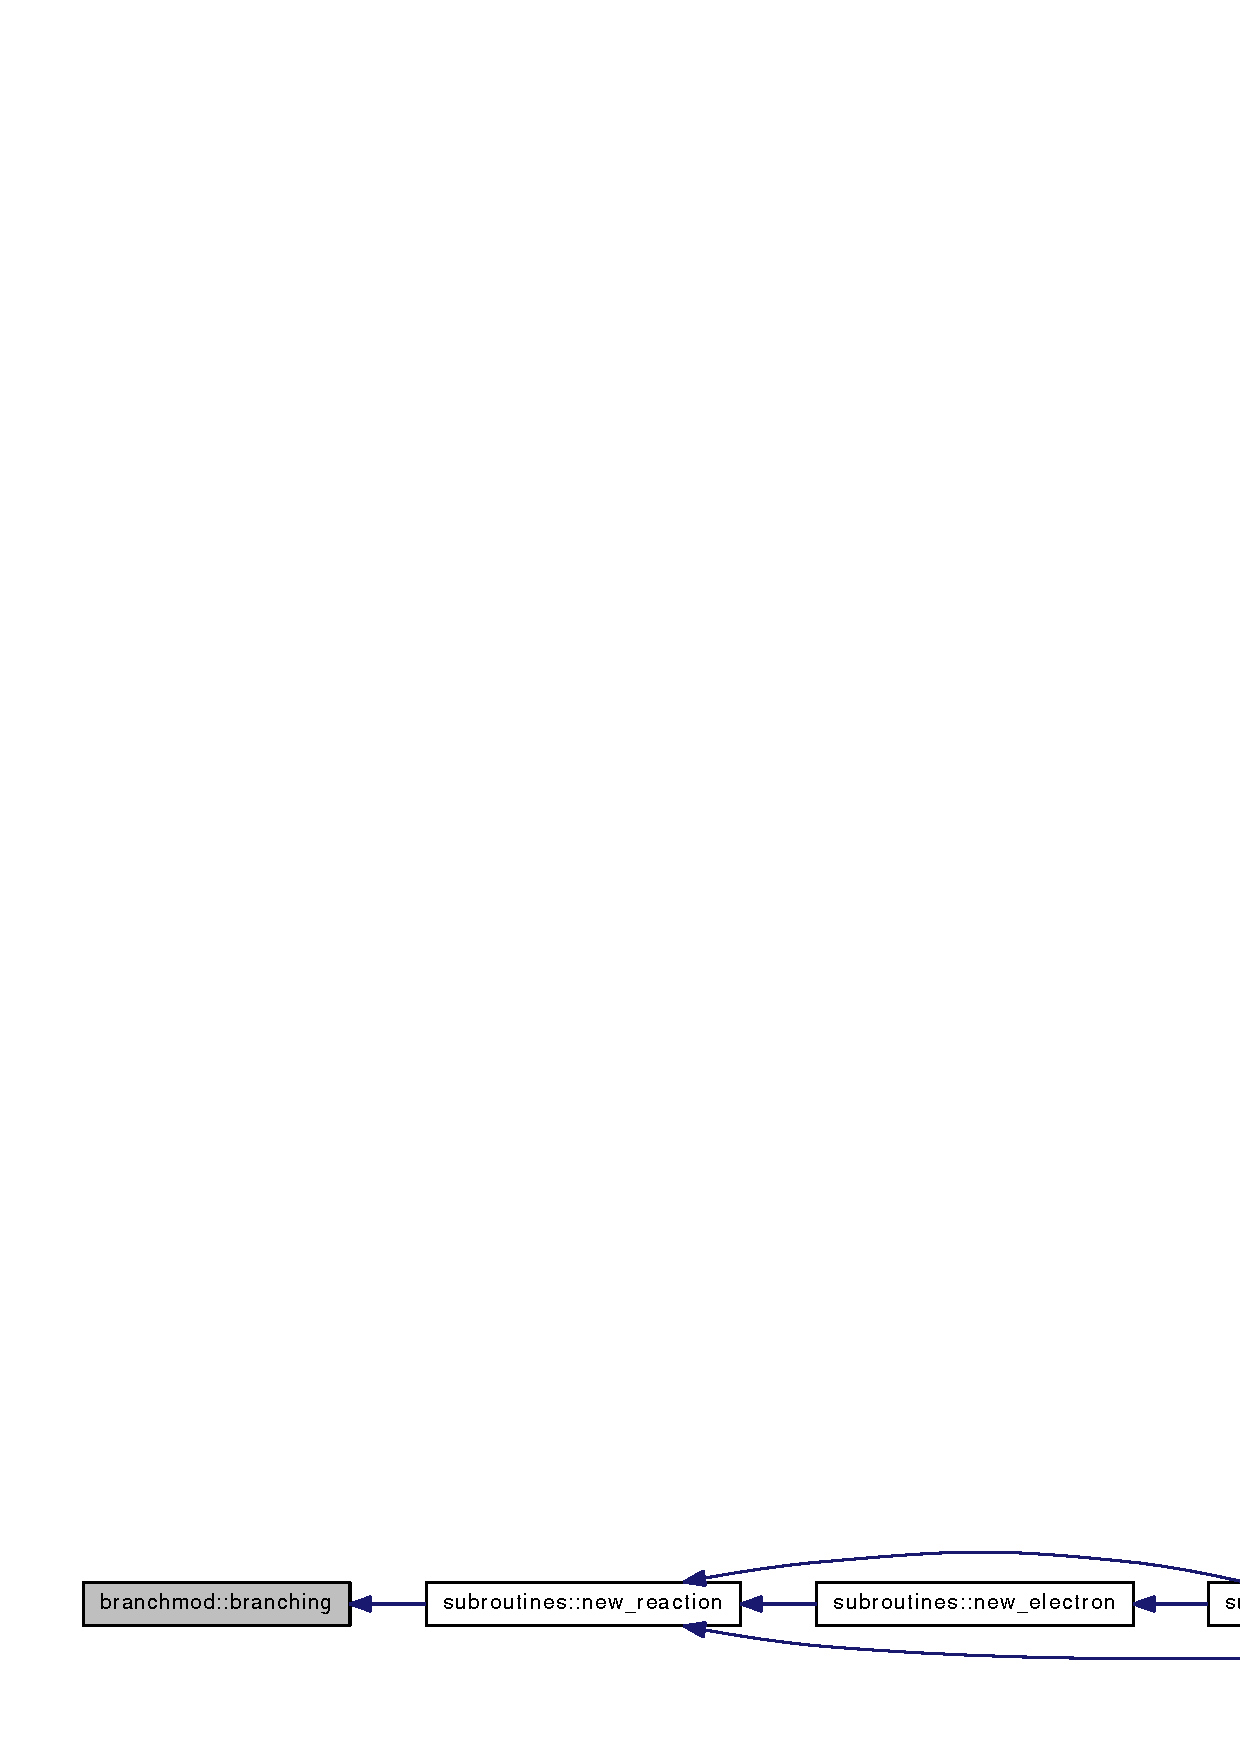
\includegraphics[width=388pt]{namespacebranchmod_afe047e9cf349dd7beea43ce0113ab24b_icgraph}
\end{center}
\end{figure}
\hypertarget{namespacebranchmod_a37435a321ae1297821d708a3891bdf0d}{
\index{branchmod@{branchmod}!bumpreaction@{bumpreaction}}
\index{bumpreaction@{bumpreaction}!branchmod@{branchmod}}
\subsubsection[{bumpreaction}]{\setlength{\rightskip}{0pt plus 5cm}subroutine branchmod::bumpreaction (INTEGER {\em id}, \/  type({\bf reaction}) {\em node})}}
\label{namespacebranchmod_a37435a321ae1297821d708a3891bdf0d}


Definition at line 168 of file branchmod.f90.\hypertarget{namespacebranchmod_a4c2d31e67892bffa2413995834db274a}{
\index{branchmod@{branchmod}!selectbranch@{selectbranch}}
\index{selectbranch@{selectbranch}!branchmod@{branchmod}}
\subsubsection[{selectbranch}]{\setlength{\rightskip}{0pt plus 5cm}subroutine branchmod::selectbranch (DOUBLE PRECISION,dimension(4),intent(in) {\em kvals}, \/  INTEGER,intent(out) {\em ndex})}}
\label{namespacebranchmod_a4c2d31e67892bffa2413995834db274a}


Definition at line 194 of file branchmod.f90.

References parameters::DEBUG.
\hypertarget{namespacebsimple}{
\section{bsimple Module Reference}
\label{namespacebsimple}\index{bsimple@{bsimple}}
}
\subsection*{Data Types}
\begin{DoxyCompactItemize}
\item 
interface \hyperlink{interfacebsimple_1_1OPERATOR_07_4_08}{OPERATOR($>$)}
\item 
interface {\bfseries OPERATOR($<$)}
\item 
interface {\bfseries OPERATOR(==)}
\end{DoxyCompactItemize}
\subsection*{Functions/Subroutines}
\begin{DoxyCompactItemize}
\item 
subroutine \hyperlink{namespacebsimple_a98a0fa9db2215d588a0a87c08065809f}{add\_\-node} (ptr, new\_\-node)
\item 
subroutine \hyperlink{namespacebsimple_ae6c8fc172ff255d4d825b1f507d9fd82}{write\_\-node} (ptr)
\item 
subroutine \hyperlink{namespacebsimple_abe5b608758a905e30ed8661e177395d6}{find\_\-node} (ptr, search, error)
\item 
subroutine \hyperlink{namespacebsimple_a021b297f11aa3649405b7931d0979be9}{find\_\-previous} (ptr, search, prevNode, leftRight, error)
\item 
subroutine \hyperlink{namespacebsimple_a11b24c82d3405b40e38891f5b2de1eeb}{find\_\-min} (ptr, search)
\item 
subroutine \hyperlink{namespacebsimple_a4cb5aa13e4c5a527c7573ccbd5234162}{delete\_\-node} (root, toDelete, prevNode, nextNode, error)
\end{DoxyCompactItemize}


\subsection{Function/Subroutine Documentation}
\hypertarget{namespacebsimple_a98a0fa9db2215d588a0a87c08065809f}{
\index{bsimple@{bsimple}!add\_\-node@{add\_\-node}}
\index{add\_\-node@{add\_\-node}!bsimple@{bsimple}}
\subsubsection[{add\_\-node}]{\setlength{\rightskip}{0pt plus 5cm}subroutine bsimple::add\_\-node (TYPE (node),pointer {\em ptr}, \/  TYPE (node),pointer {\em new\_\-node})}}
\label{namespacebsimple_a98a0fa9db2215d588a0a87c08065809f}


Definition at line 48 of file bsimple.f90.

Referenced by subroutines::init\_\-node(), main(), and subroutines::new\_\-reaction().

Here is the caller graph for this function:\nopagebreak
\begin{figure}[H]
\begin{center}
\leavevmode
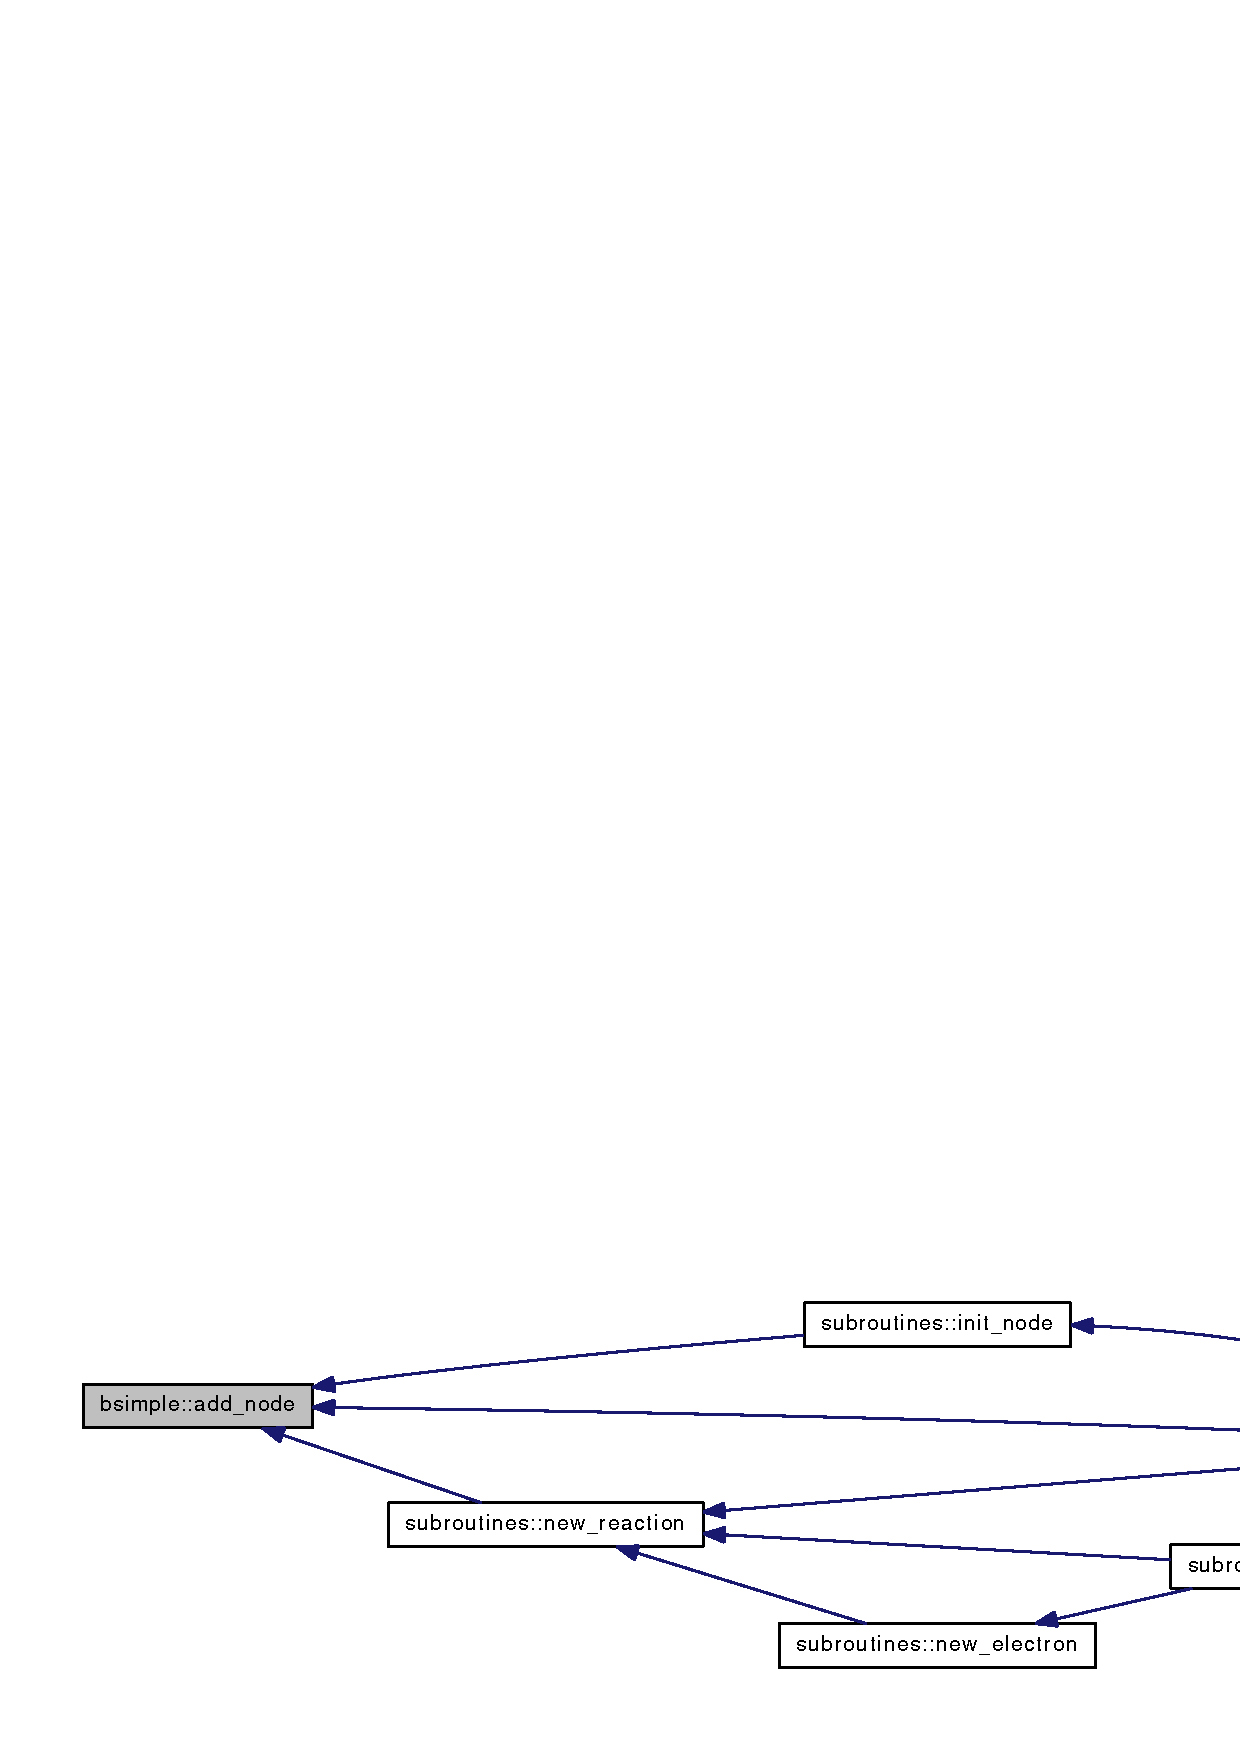
\includegraphics[width=379pt]{namespacebsimple_a98a0fa9db2215d588a0a87c08065809f_icgraph}
\end{center}
\end{figure}
\hypertarget{namespacebsimple_a4cb5aa13e4c5a527c7573ccbd5234162}{
\index{bsimple@{bsimple}!delete\_\-node@{delete\_\-node}}
\index{delete\_\-node@{delete\_\-node}!bsimple@{bsimple}}
\subsubsection[{delete\_\-node}]{\setlength{\rightskip}{0pt plus 5cm}subroutine bsimple::delete\_\-node (TYPE (node),pointer {\em root}, \/  TYPE (node),pointer {\em toDelete}, \/  TYPE (node),pointer {\em prevNode}, \/  TYPE (node),pointer {\em nextNode}, \/  INTEGER {\em error})}}
\label{namespacebsimple_a4cb5aa13e4c5a527c7573ccbd5234162}


Definition at line 219 of file bsimple.f90.

References parameters::DEBUG, find\_\-min(), and write\_\-node().

Referenced by main(), and subroutines::new\_\-reaction().

Here is the call graph for this function:\nopagebreak
\begin{figure}[H]
\begin{center}
\leavevmode
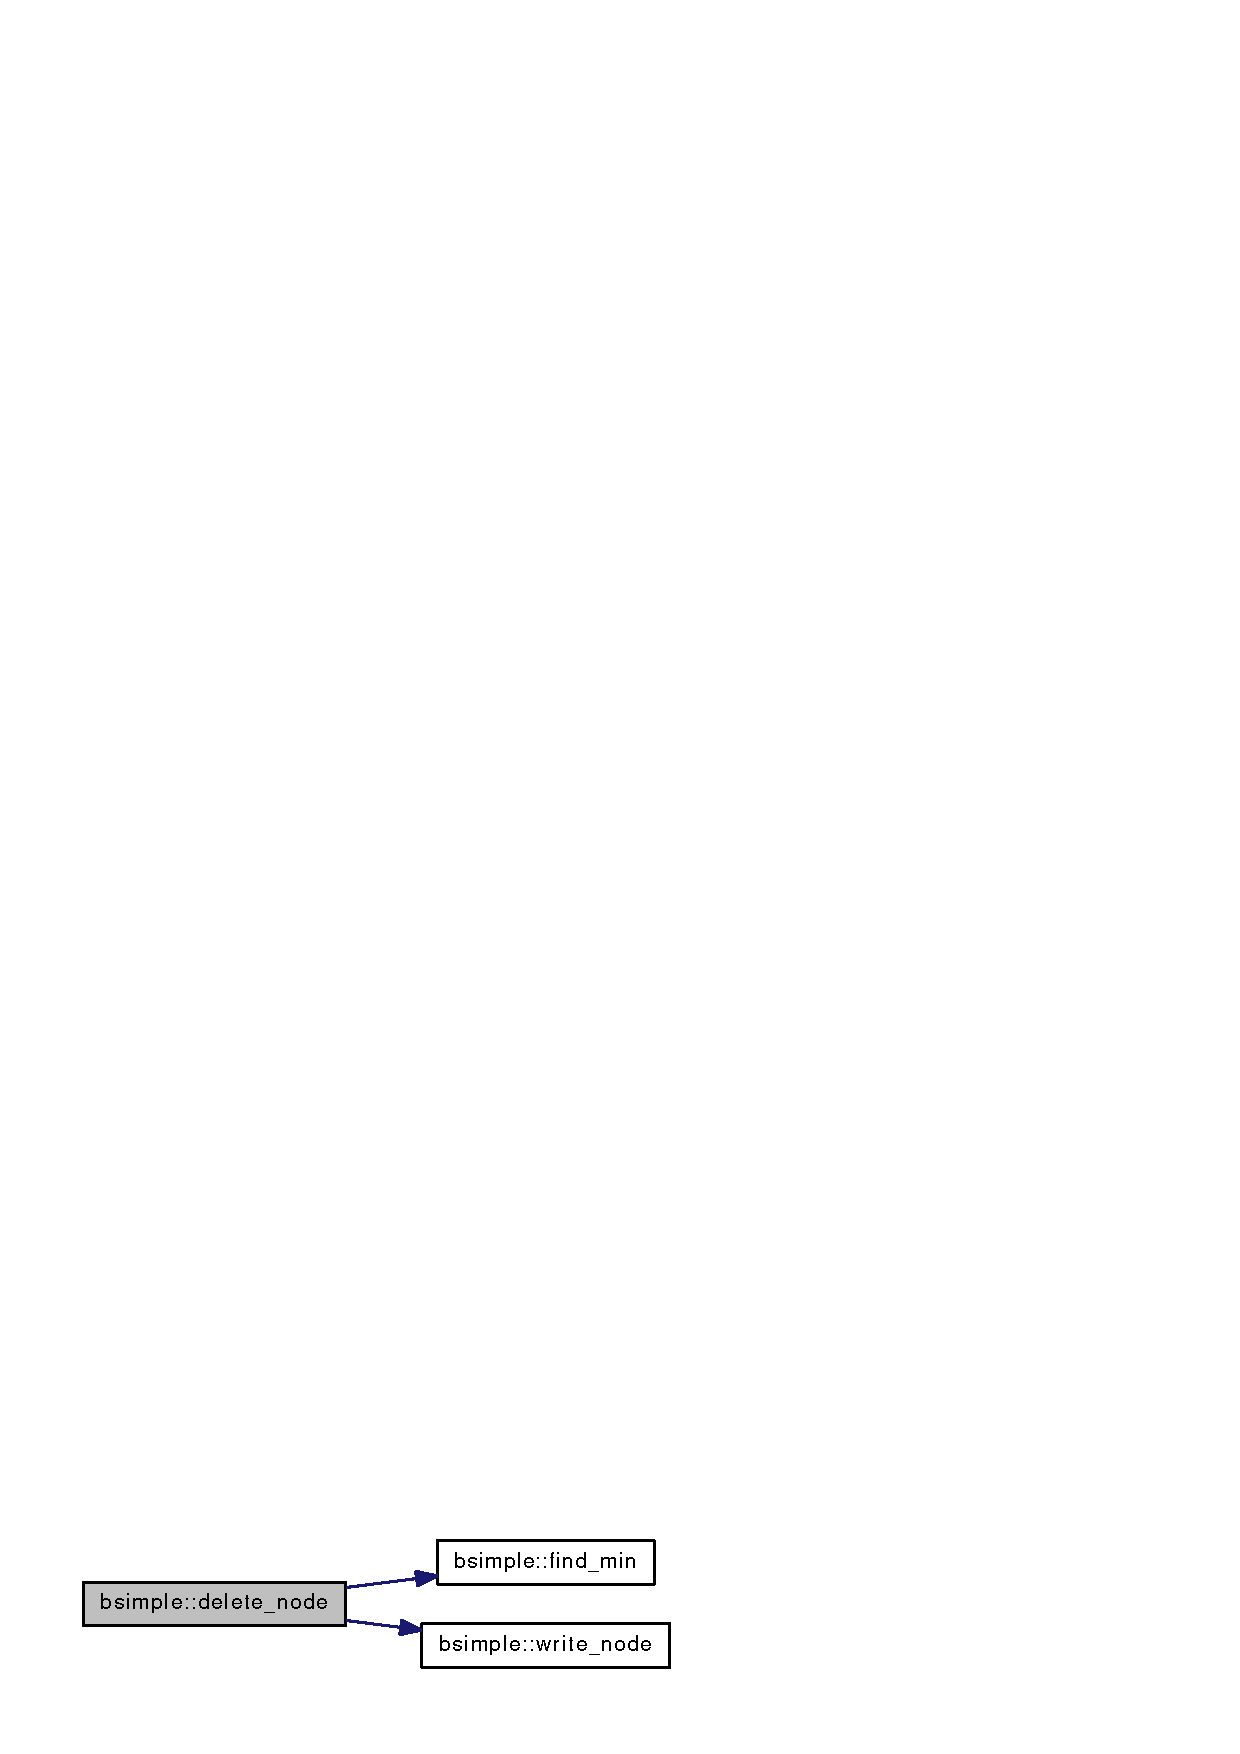
\includegraphics[width=163pt]{namespacebsimple_a4cb5aa13e4c5a527c7573ccbd5234162_cgraph}
\end{center}
\end{figure}


Here is the caller graph for this function:\nopagebreak
\begin{figure}[H]
\begin{center}
\leavevmode
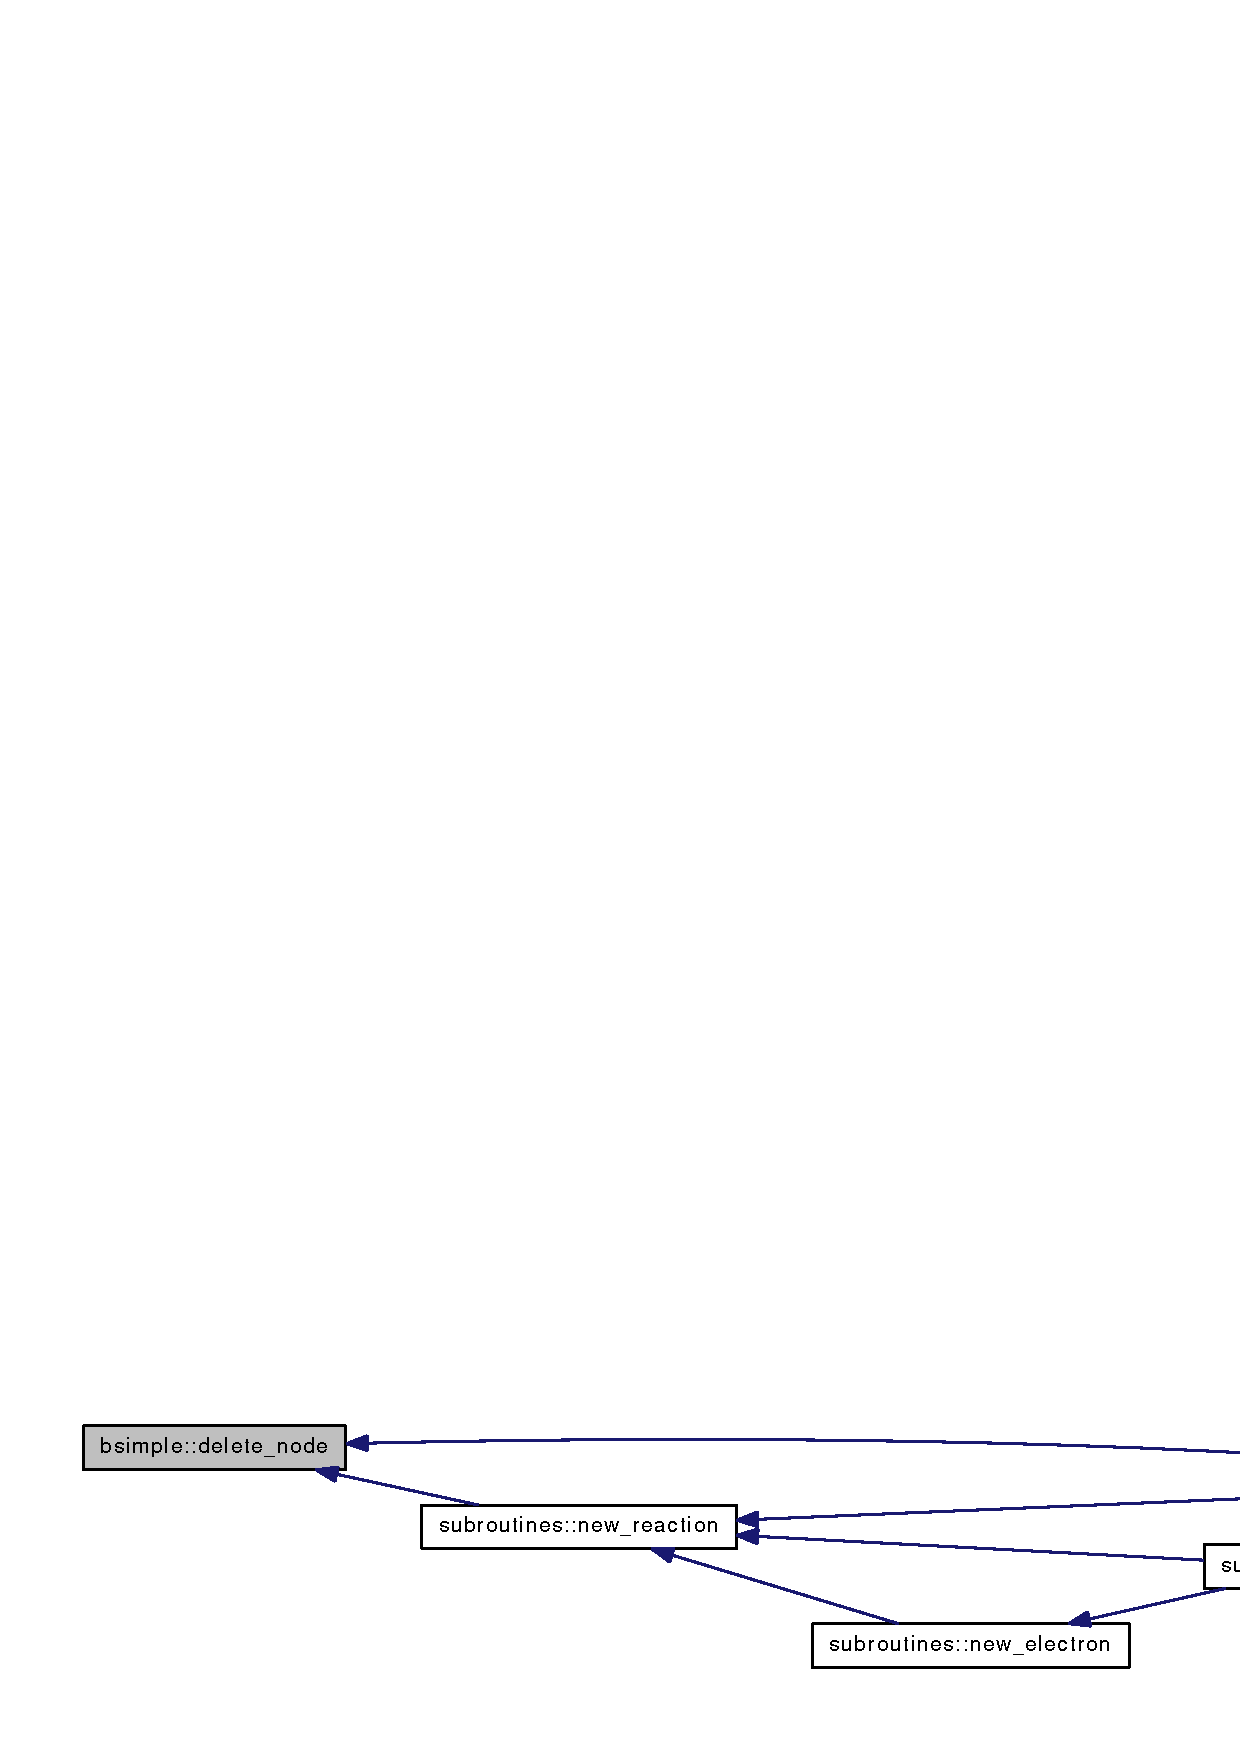
\includegraphics[width=387pt]{namespacebsimple_a4cb5aa13e4c5a527c7573ccbd5234162_icgraph}
\end{center}
\end{figure}
\hypertarget{namespacebsimple_a11b24c82d3405b40e38891f5b2de1eeb}{
\index{bsimple@{bsimple}!find\_\-min@{find\_\-min}}
\index{find\_\-min@{find\_\-min}!bsimple@{bsimple}}
\subsubsection[{find\_\-min}]{\setlength{\rightskip}{0pt plus 5cm}subroutine bsimple::find\_\-min (TYPE (node),pointer {\em ptr}, \/  TYPE (node),pointer {\em search})}}
\label{namespacebsimple_a11b24c82d3405b40e38891f5b2de1eeb}


Definition at line 207 of file bsimple.f90.

Referenced by delete\_\-node(), and main().

Here is the caller graph for this function:\nopagebreak
\begin{figure}[H]
\begin{center}
\leavevmode
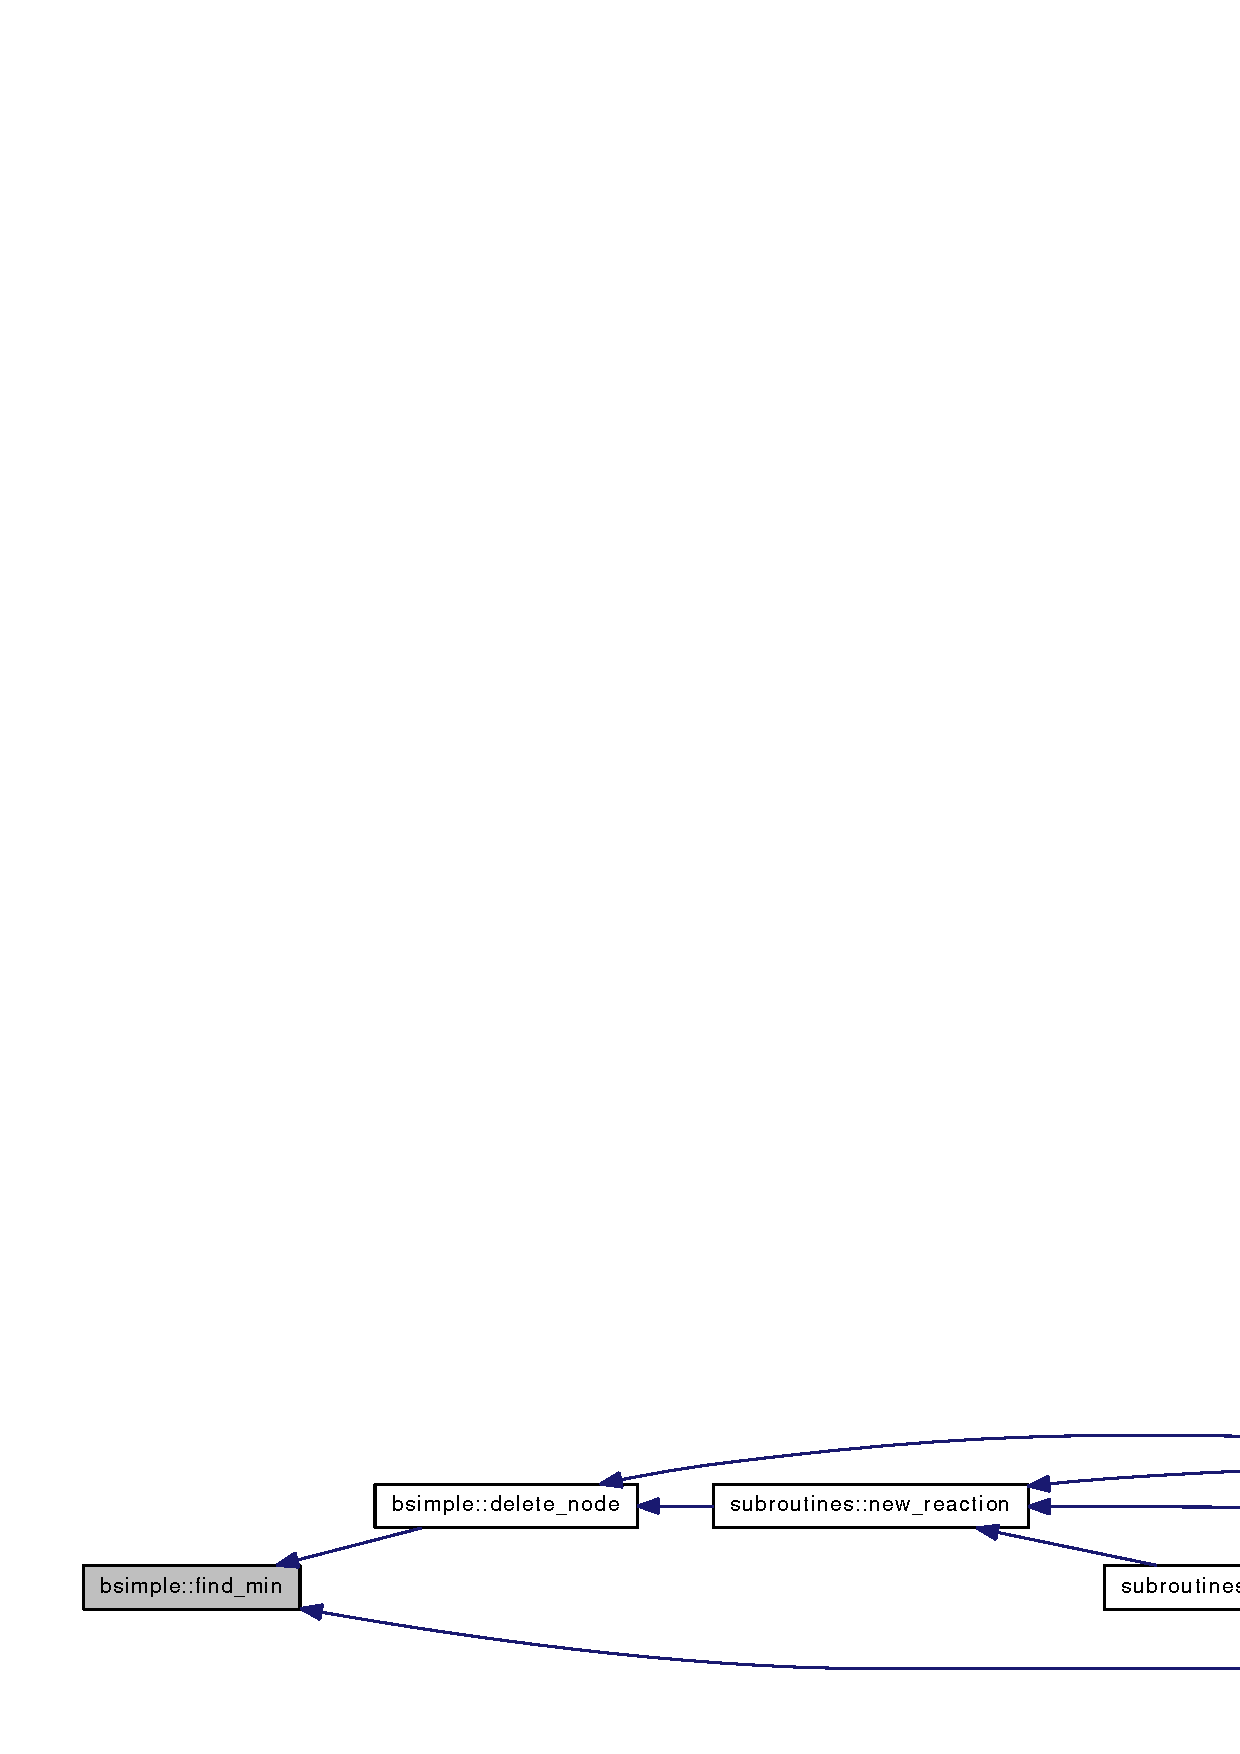
\includegraphics[width=420pt]{namespacebsimple_a11b24c82d3405b40e38891f5b2de1eeb_icgraph}
\end{center}
\end{figure}
\hypertarget{namespacebsimple_abe5b608758a905e30ed8661e177395d6}{
\index{bsimple@{bsimple}!find\_\-node@{find\_\-node}}
\index{find\_\-node@{find\_\-node}!bsimple@{bsimple}}
\subsubsection[{find\_\-node}]{\setlength{\rightskip}{0pt plus 5cm}subroutine bsimple::find\_\-node (TYPE (node),pointer {\em ptr}, \/  TYPE (node),pointer {\em search}, \/  INTEGER {\em error})}}
\label{namespacebsimple_abe5b608758a905e30ed8661e177395d6}


Definition at line 102 of file bsimple.f90.\hypertarget{namespacebsimple_a021b297f11aa3649405b7931d0979be9}{
\index{bsimple@{bsimple}!find\_\-previous@{find\_\-previous}}
\index{find\_\-previous@{find\_\-previous}!bsimple@{bsimple}}
\subsubsection[{find\_\-previous}]{\setlength{\rightskip}{0pt plus 5cm}subroutine bsimple::find\_\-previous (TYPE (node),pointer {\em ptr}, \/  TYPE (node),pointer {\em search}, \/  TYPE (node),pointer {\em prevNode}, \/  INTEGER {\em leftRight}, \/  INTEGER {\em error})}}
\label{namespacebsimple_a021b297f11aa3649405b7931d0979be9}


Definition at line 132 of file bsimple.f90.

References write\_\-node().

Here is the call graph for this function:\nopagebreak
\begin{figure}[H]
\begin{center}
\leavevmode
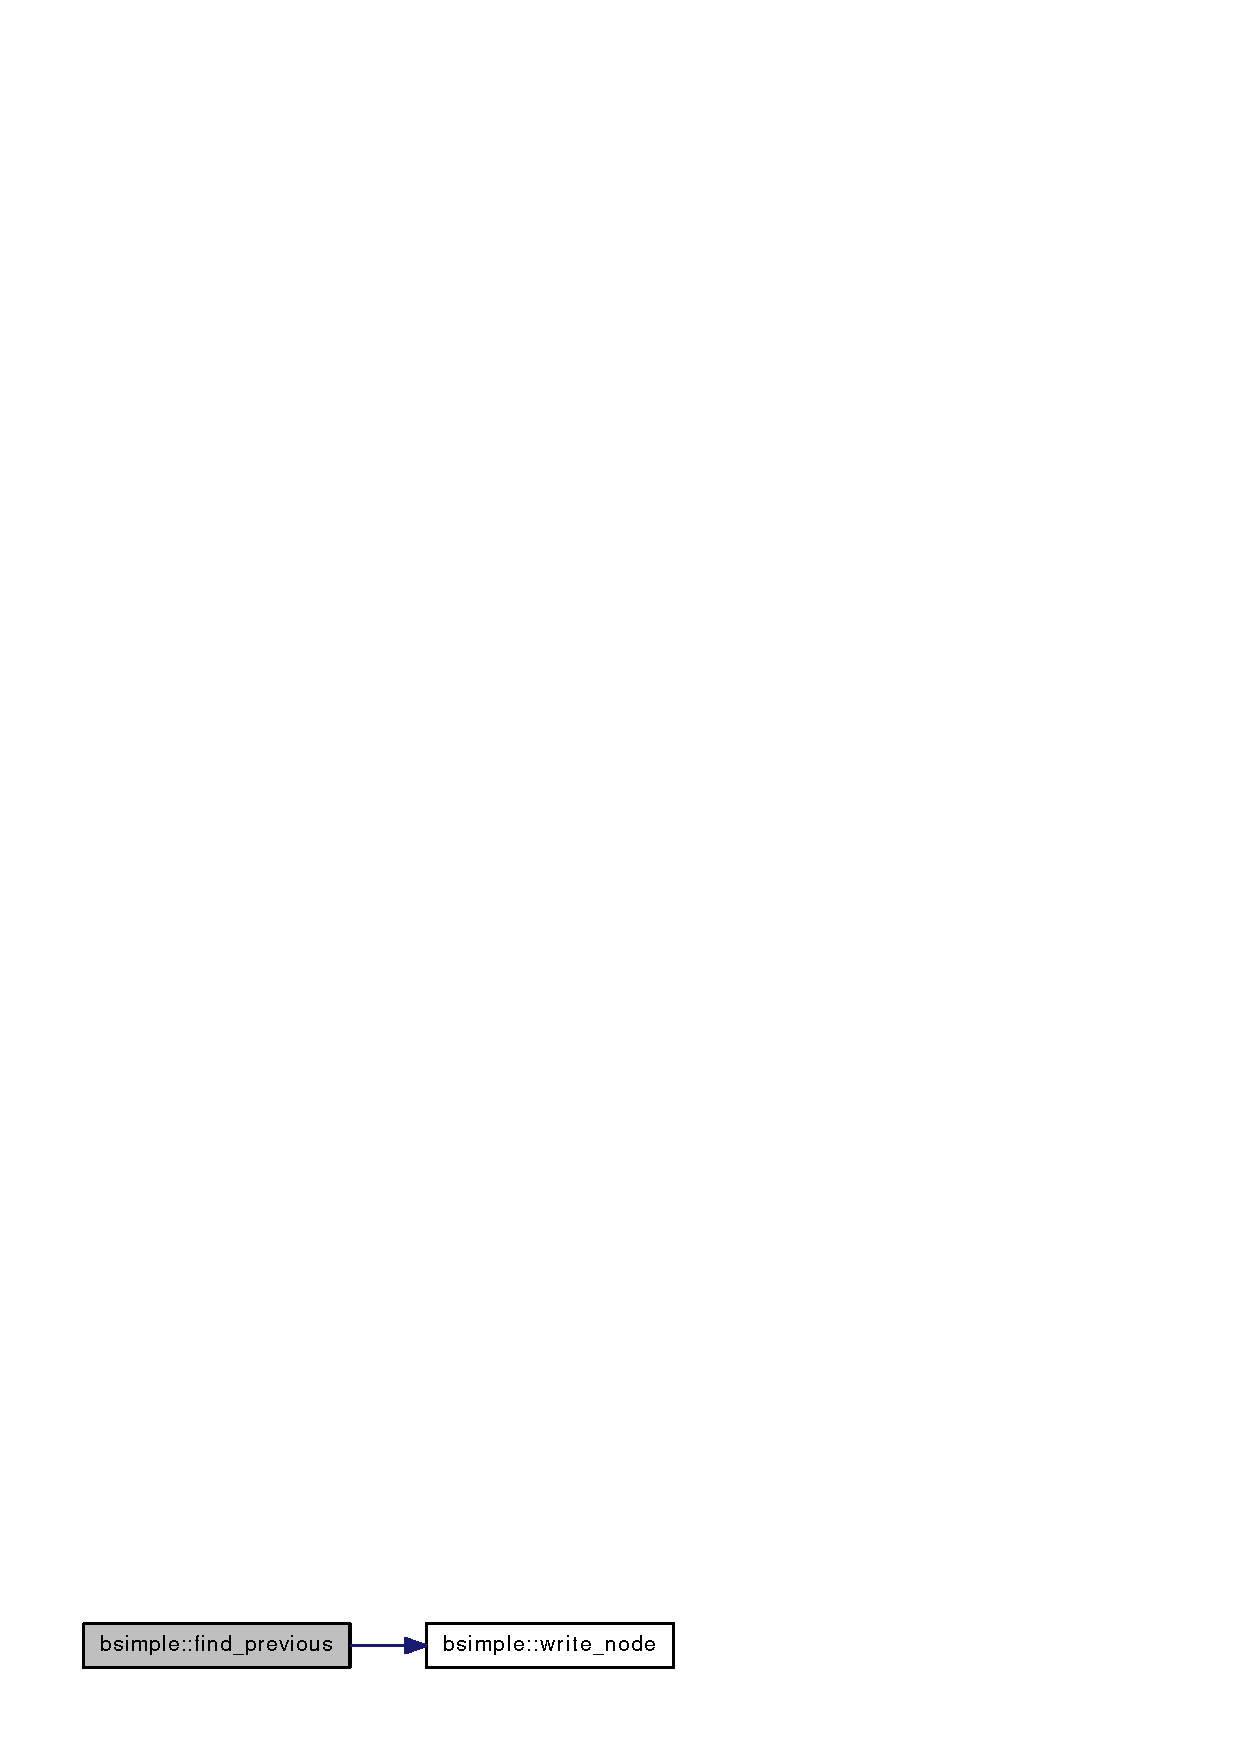
\includegraphics[width=164pt]{namespacebsimple_a021b297f11aa3649405b7931d0979be9_cgraph}
\end{center}
\end{figure}
\hypertarget{namespacebsimple_ae6c8fc172ff255d4d825b1f507d9fd82}{
\index{bsimple@{bsimple}!write\_\-node@{write\_\-node}}
\index{write\_\-node@{write\_\-node}!bsimple@{bsimple}}
\subsubsection[{write\_\-node}]{\setlength{\rightskip}{0pt plus 5cm}subroutine bsimple::write\_\-node (TYPE (node),pointer {\em ptr})}}
\label{namespacebsimple_ae6c8fc172ff255d4d825b1f507d9fd82}


Definition at line 80 of file bsimple.f90.

Referenced by delete\_\-node(), and find\_\-previous().

Here is the caller graph for this function:\nopagebreak
\begin{figure}[H]
\begin{center}
\leavevmode
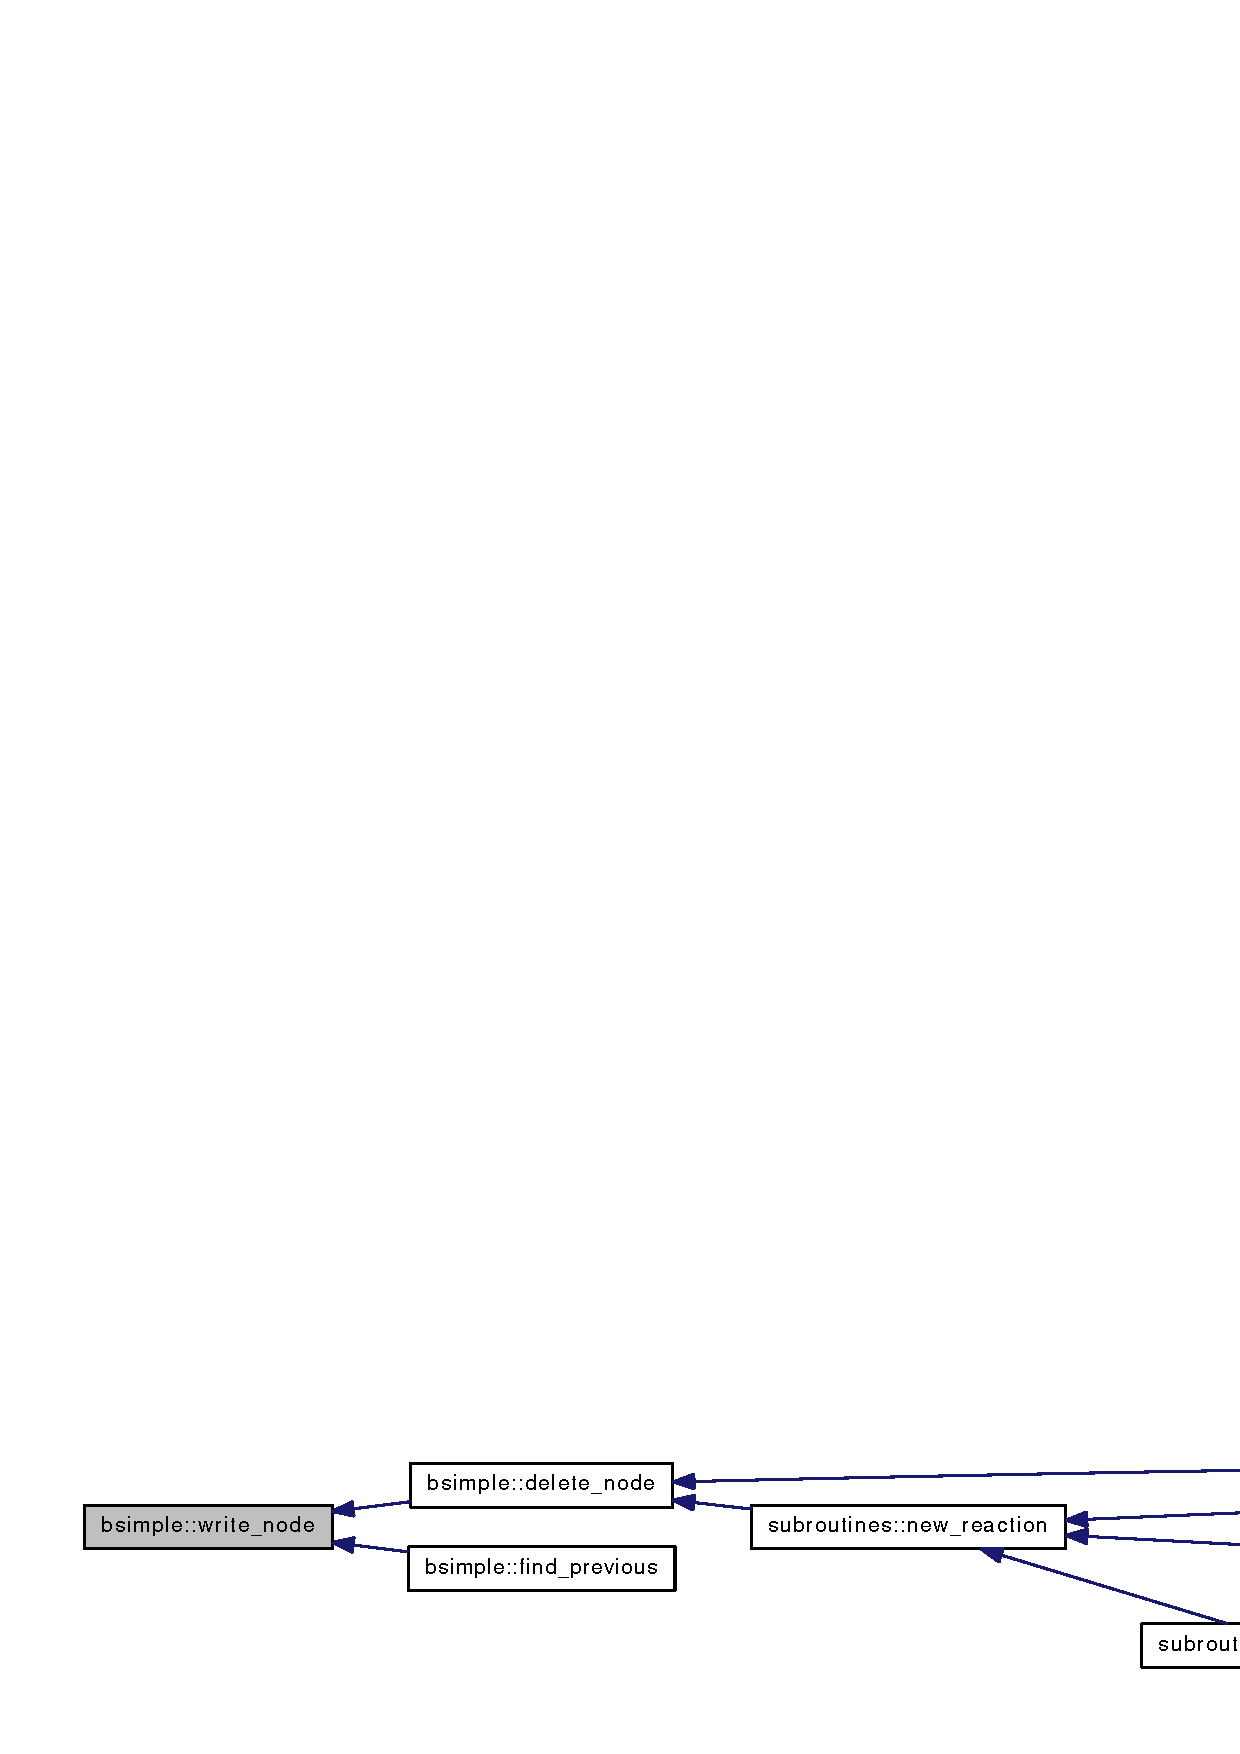
\includegraphics[width=420pt]{namespacebsimple_ae6c8fc172ff255d4d825b1f507d9fd82_icgraph}
\end{center}
\end{figure}

\hypertarget{namespacefunctiondefs}{
\section{functiondefs Module Reference}
\label{namespacefunctiondefs}\index{functiondefs@{functiondefs}}
}
\subsection*{Functions/Subroutines}
\begin{DoxyCompactItemize}
\item 
DOUBLE PRECISION \hyperlink{namespacefunctiondefs_ae9b1c95ccb465d122918ab89da45aed7}{arrhenius} (a, b, c)
\item 
DOUBLE PRECISION \hyperlink{namespacefunctiondefs_ad75756612cb12ba4983414cdc520f6a1}{green\_\-mcneal} (energy, a, j, nu, omega, z, i)
\item 
DOUBLE PRECISION \hyperlink{namespacefunctiondefs_a9cd4ed9f980bd43386e7de1e3e35c79c}{a\_\-gs} (energy, k, k\_\-b, j, j\_\-b, j\_\-c)
\item 
DOUBLE PRECISION \hyperlink{namespacefunctiondefs_adae12a3980d4e2bd5fe6277c91988474}{gamma\_\-gs} (energy, gamma\_\-s, gamma\_\-b)
\item 
DOUBLE PRECISION \hyperlink{namespacefunctiondefs_a5e1c4c25a7352f149e1f18854c37930f}{t\_\-0\_\-gs} (energy, t\_\-a, t\_\-b, t\_\-s)
\item 
DOUBLE PRECISION \hyperlink{namespacefunctiondefs_a7beb6f6af6e15afda97da88dde407655}{t\_\-max\_\-gs} (energy, i)
\item 
DOUBLE PRECISION \hyperlink{namespacefunctiondefs_a64cc5970914d70f20e127be3722f11bb}{green\_\-sawada} (a, gamma\_\-fac, t\_\-max, t\_\-0)
\item 
REAL \hyperlink{namespacefunctiondefs_abb5f2d51b3f8b637e0d17ad8c21db948}{ne\_\-mg} (gamma\_\-fac, t\_\-max, t\_\-0)
\item 
subroutine \hyperlink{namespacefunctiondefs_a93c18b11591055e1e1275c6dc7b2ab26}{magic} (eps, b, c2, s2, theta)
\item 
DOUBLE PRECISION \hyperlink{namespacefunctiondefs_a34160b04b7880953967f273645a835c5}{b\_\-magic} (rn, a, rho)
\item 
DOUBLE PRECISION \hyperlink{namespacefunctiondefs_abf4df469161d4f4092a1a538a20ebf1d}{au} (z1, z2)
\item 
DOUBLE PRECISION \hyperlink{namespacefunctiondefs_ac20c2b09d0408eb23b226af7f8f7361a}{eps} (en, z1, z2, m1, m2, au)
\item 
DOUBLE PRECISION \hyperlink{namespacefunctiondefs_aa92057c8da0a7ce374166fed435ea54f}{mass\_\-fac} (m1, m2)
\item 
DOUBLE PRECISION \hyperlink{namespacefunctiondefs_a529a6bcbb0305c32f0275aa85d4303e8}{t\_\-coll} (e, mf, s2)
\item 
DOUBLE PRECISION \hyperlink{namespacefunctiondefs_abeba54805575687a8d1db47decf4790e}{lab\_\-theta} (cmtheta, m1, m2)
\item 
DOUBLE PRECISION \hyperlink{namespacefunctiondefs_a80d99fe52a1cb5856694596955d8aeb9}{sneps} (eps)
\item 
DOUBLE PRECISION \hyperlink{namespacefunctiondefs_a78455979576075ad68feb125604462bc}{sne} (sneps, z1, z2, m1, m2)
\item 
DOUBLE PRECISION \hyperlink{namespacefunctiondefs_ae52b03b9e83dd8f46fd7532fb105850b}{pelsig} (energy, sne, mf)
\item 
DOUBLE PRECISION \hyperlink{namespacefunctiondefs_a7a31d88fad502937338eafac9a574fec}{greendutta} (energy, w, f, o, a, b)
\item 
DOUBLE PRECISION \hyperlink{namespacefunctiondefs_a5486e5e48a1c871c2ec9d5bc03406ea5}{pjgsigma} (energy, f, w, c, a, b)
\end{DoxyCompactItemize}


\subsection{Function/Subroutine Documentation}
\hypertarget{namespacefunctiondefs_a9cd4ed9f980bd43386e7de1e3e35c79c}{
\index{functiondefs@{functiondefs}!a\_\-gs@{a\_\-gs}}
\index{a\_\-gs@{a\_\-gs}!functiondefs@{functiondefs}}
\subsubsection[{a\_\-gs}]{\setlength{\rightskip}{0pt plus 5cm}DOUBLE PRECISION functiondefs::a\_\-gs (DOUBLE PRECISION,intent(in) {\em energy}, \/  DOUBLE PRECISION,intent(in) {\em k}, \/  DOUBLE PRECISION,intent(in) {\em k\_\-b}, \/  DOUBLE PRECISION,intent(in) {\em j}, \/  DOUBLE PRECISION,intent(in) {\em j\_\-b}, \/  DOUBLE PRECISION,intent(in) {\em j\_\-c})}}
\label{namespacefunctiondefs_a9cd4ed9f980bd43386e7de1e3e35c79c}


Definition at line 55 of file functiondefs.f90.

Referenced by subroutines::esigma\_\-suite().

Here is the caller graph for this function:\nopagebreak
\begin{figure}[H]
\begin{center}
\leavevmode
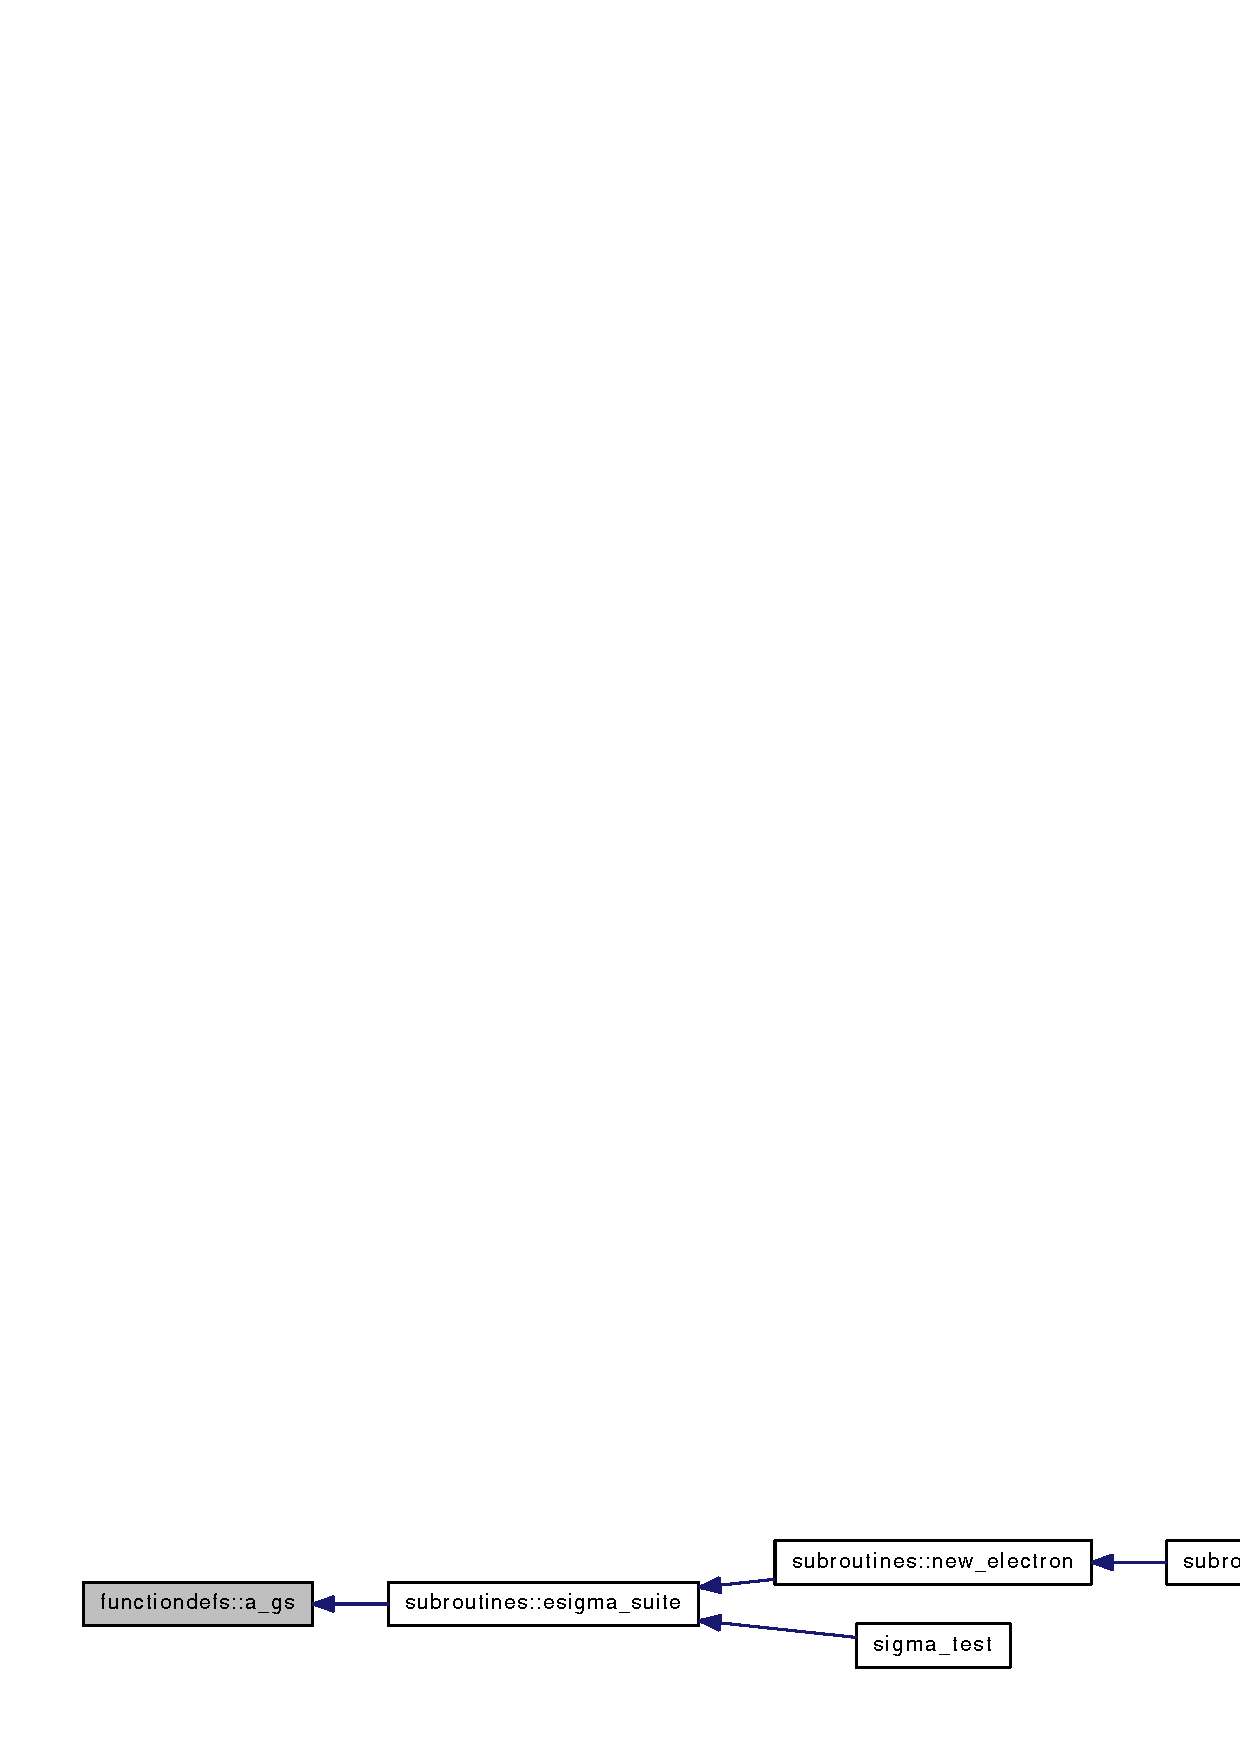
\includegraphics[width=378pt]{namespacefunctiondefs_a9cd4ed9f980bd43386e7de1e3e35c79c_icgraph}
\end{center}
\end{figure}
\hypertarget{namespacefunctiondefs_ae9b1c95ccb465d122918ab89da45aed7}{
\index{functiondefs@{functiondefs}!arrhenius@{arrhenius}}
\index{arrhenius@{arrhenius}!functiondefs@{functiondefs}}
\subsubsection[{arrhenius}]{\setlength{\rightskip}{0pt plus 5cm}DOUBLE PRECISION functiondefs::arrhenius (DOUBLE PRECISION {\em a}, \/  DOUBLE PRECISION {\em b}, \/  DOUBLE PRECISION {\em c})}}
\label{namespacefunctiondefs_ae9b1c95ccb465d122918ab89da45aed7}


Definition at line 5 of file functiondefs.f90.

References parameters::KIN\_\-TEMP.\hypertarget{namespacefunctiondefs_abf4df469161d4f4092a1a538a20ebf1d}{
\index{functiondefs@{functiondefs}!au@{au}}
\index{au@{au}!functiondefs@{functiondefs}}
\subsubsection[{au}]{\setlength{\rightskip}{0pt plus 5cm}DOUBLE PRECISION functiondefs::au (DOUBLE PRECISION,intent(in) {\em z1}, \/  DOUBLE PRECISION,intent(in) {\em z2})}}
\label{namespacefunctiondefs_abf4df469161d4f4092a1a538a20ebf1d}


Definition at line 355 of file functiondefs.f90.

References parameters::A0.

Referenced by subroutines::elastic\_\-event(), and subroutines::psigma\_\-suite().

Here is the caller graph for this function:\nopagebreak
\begin{figure}[H]
\begin{center}
\leavevmode
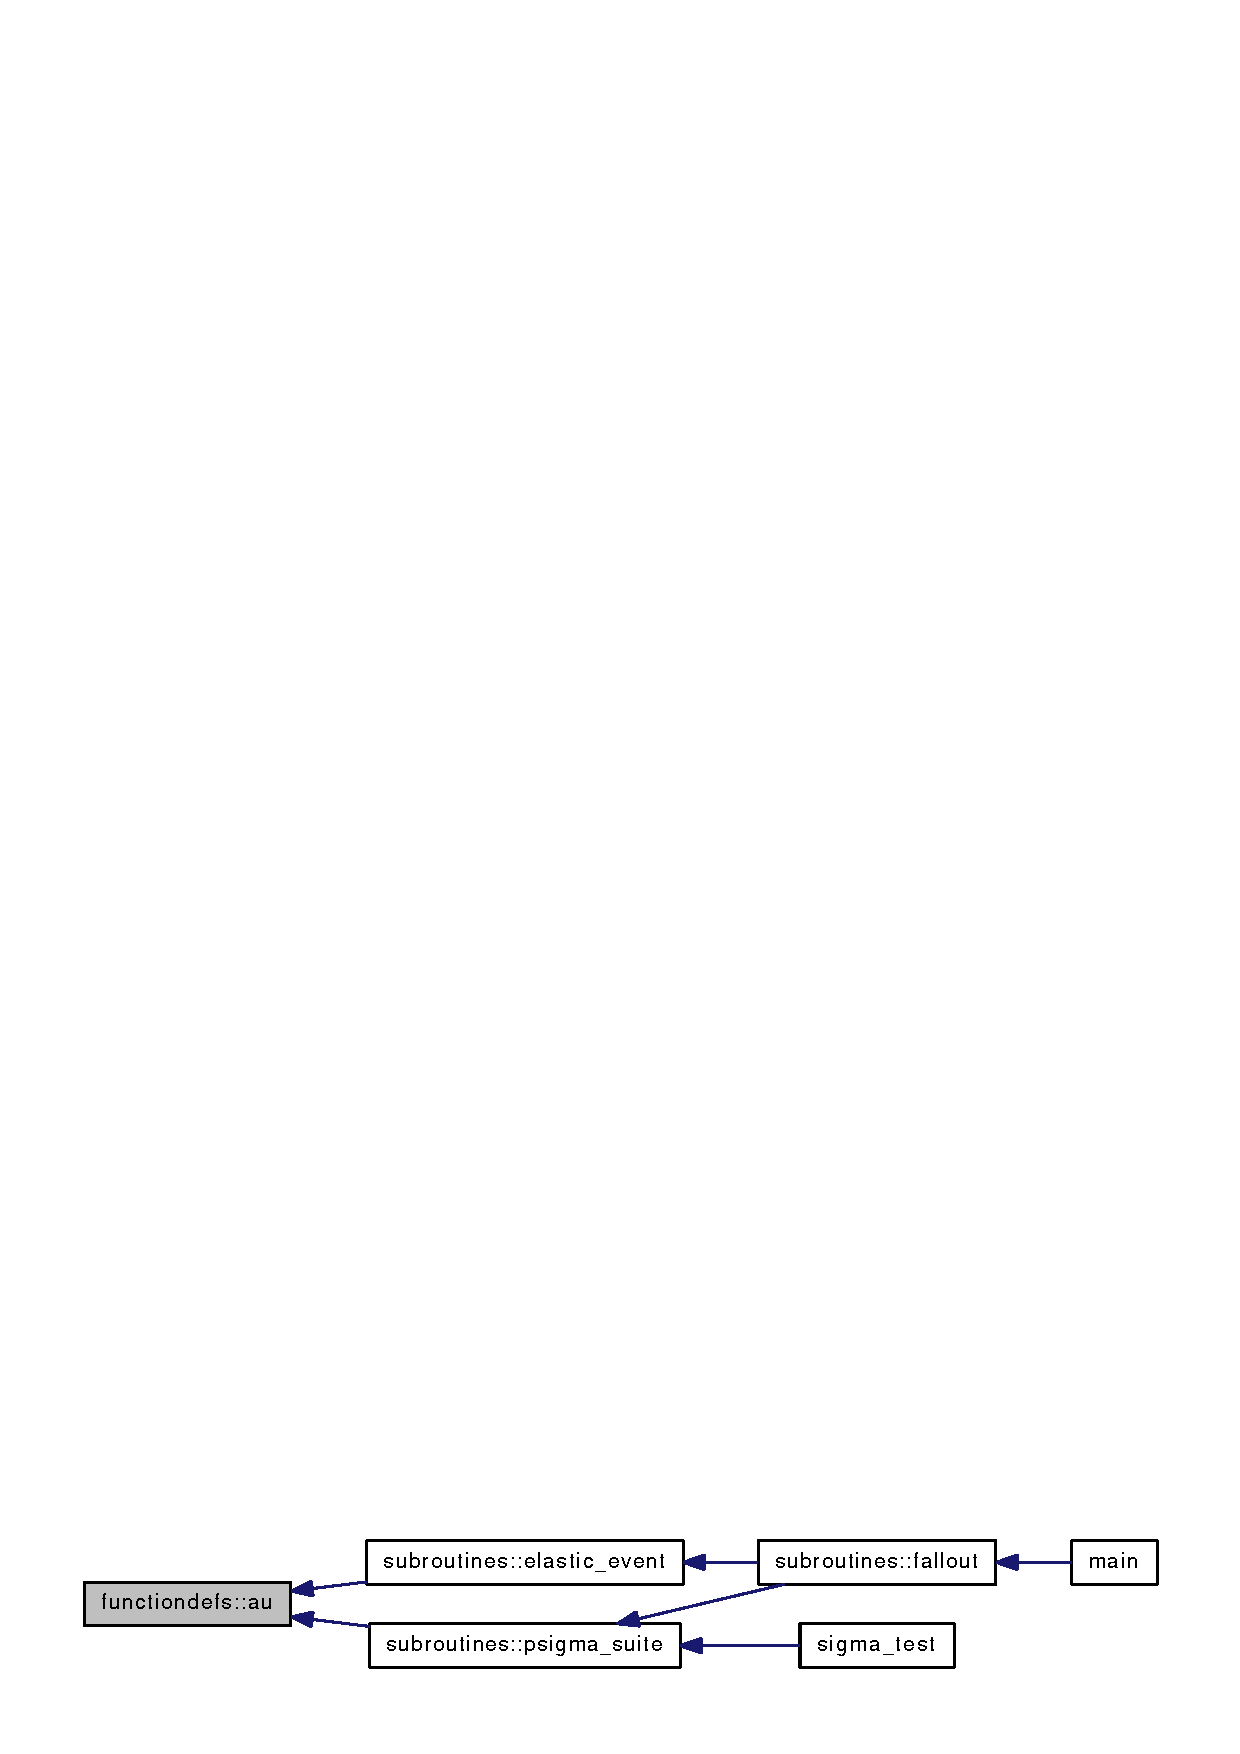
\includegraphics[width=280pt]{namespacefunctiondefs_abf4df469161d4f4092a1a538a20ebf1d_icgraph}
\end{center}
\end{figure}
\hypertarget{namespacefunctiondefs_a34160b04b7880953967f273645a835c5}{
\index{functiondefs@{functiondefs}!b\_\-magic@{b\_\-magic}}
\index{b\_\-magic@{b\_\-magic}!functiondefs@{functiondefs}}
\subsubsection[{b\_\-magic}]{\setlength{\rightskip}{0pt plus 5cm}DOUBLE PRECISION functiondefs::b\_\-magic (DOUBLE PRECISION,intent(in) {\em rn}, \/  DOUBLE PRECISION,intent(in) {\em a}, \/  DOUBLE PRECISION,intent(in) {\em rho})}}
\label{namespacefunctiondefs_a34160b04b7880953967f273645a835c5}


Definition at line 326 of file functiondefs.f90.

Referenced by subroutines::elastic\_\-event().

Here is the caller graph for this function:\nopagebreak
\begin{figure}[H]
\begin{center}
\leavevmode
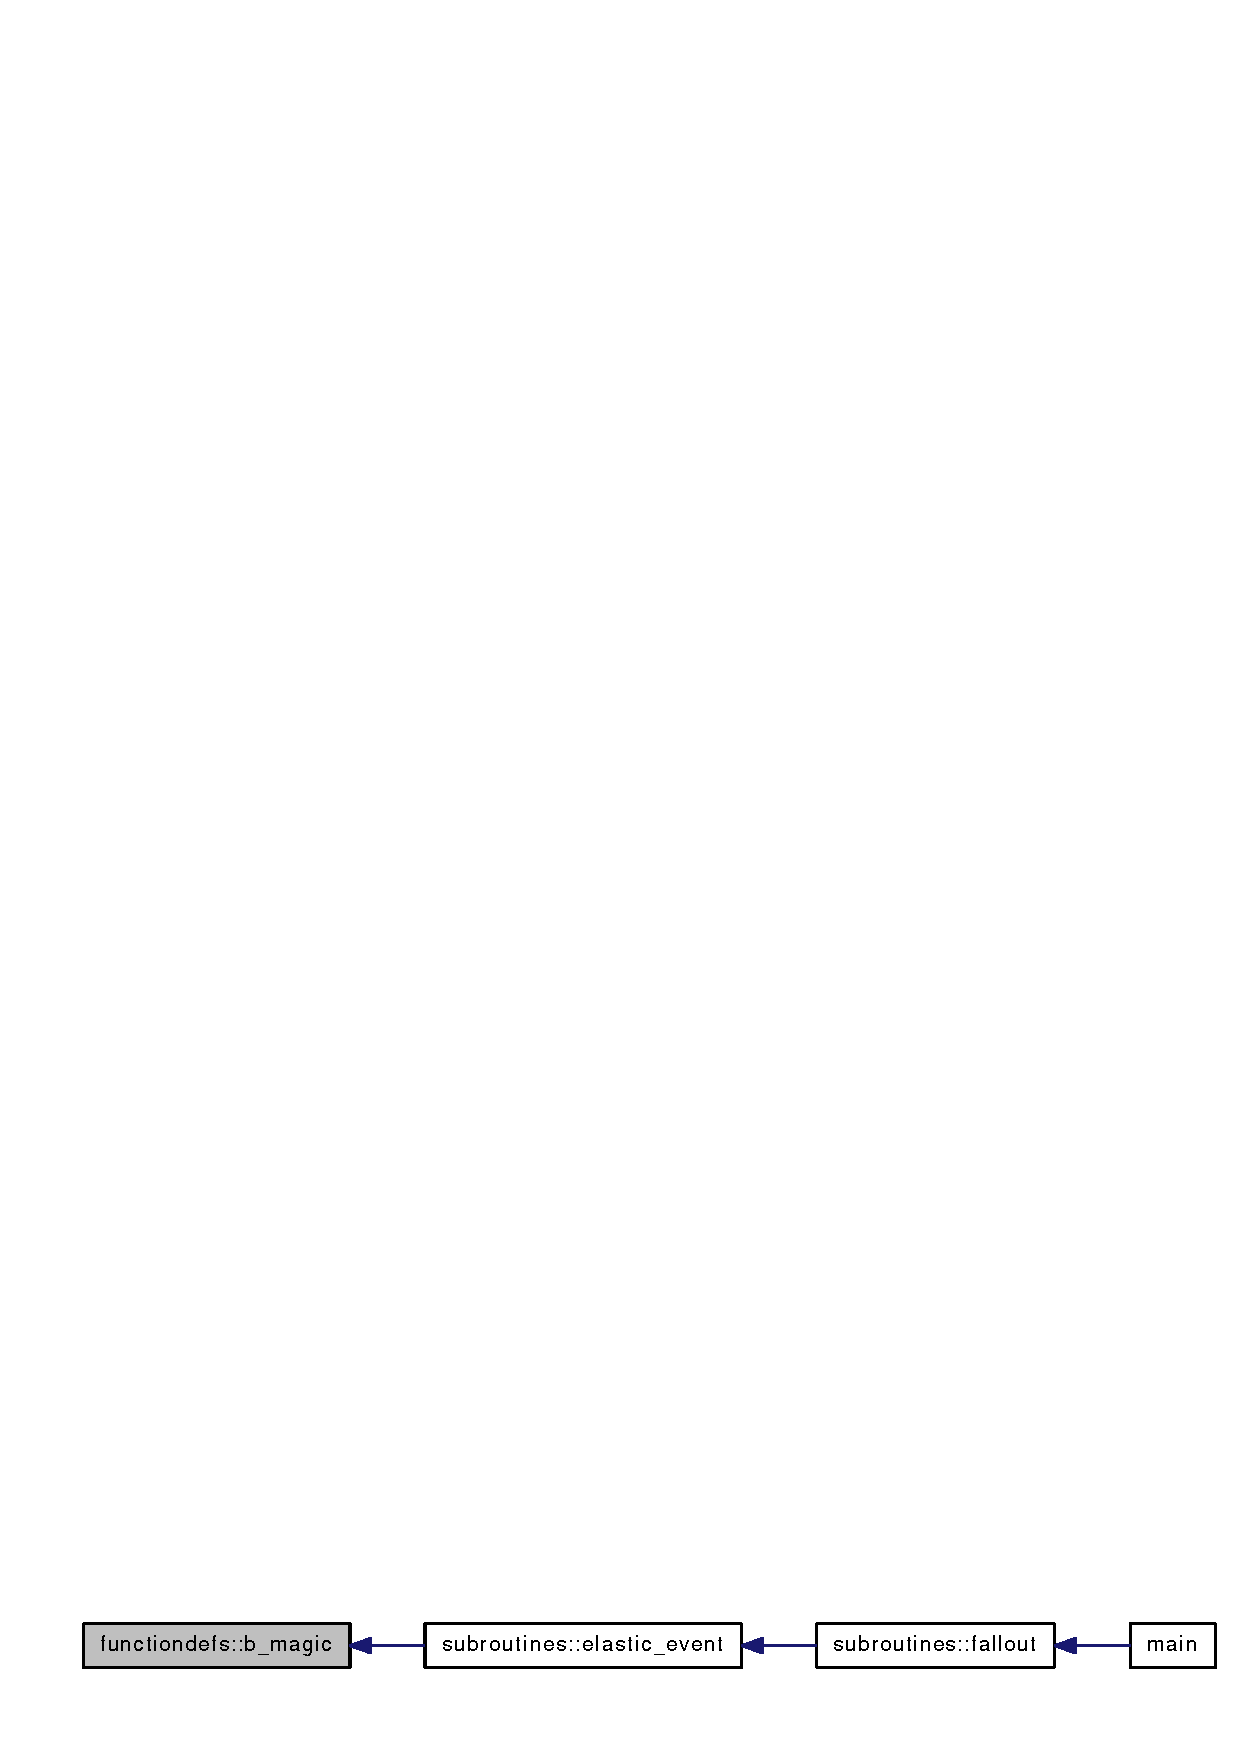
\includegraphics[width=294pt]{namespacefunctiondefs_a34160b04b7880953967f273645a835c5_icgraph}
\end{center}
\end{figure}
\hypertarget{namespacefunctiondefs_ac20c2b09d0408eb23b226af7f8f7361a}{
\index{functiondefs@{functiondefs}!eps@{eps}}
\index{eps@{eps}!functiondefs@{functiondefs}}
\subsubsection[{eps}]{\setlength{\rightskip}{0pt plus 5cm}DOUBLE PRECISION functiondefs::eps (DOUBLE PRECISION,pointer {\em en}, \/  DOUBLE PRECISION,intent(in) {\em z1}, \/  DOUBLE PRECISION,intent(in) {\em z2}, \/  DOUBLE PRECISION,intent(in) {\em m1}, \/  DOUBLE PRECISION,intent(in) {\em m2}, \/  DOUBLE PRECISION,intent(in) {\em au})}}
\label{namespacefunctiondefs_ac20c2b09d0408eb23b226af7f8f7361a}


Definition at line 376 of file functiondefs.f90.

References parameters::ECHARG2.

Referenced by subroutines::elastic\_\-event(), and subroutines::psigma\_\-suite().

Here is the caller graph for this function:\nopagebreak
\begin{figure}[H]
\begin{center}
\leavevmode
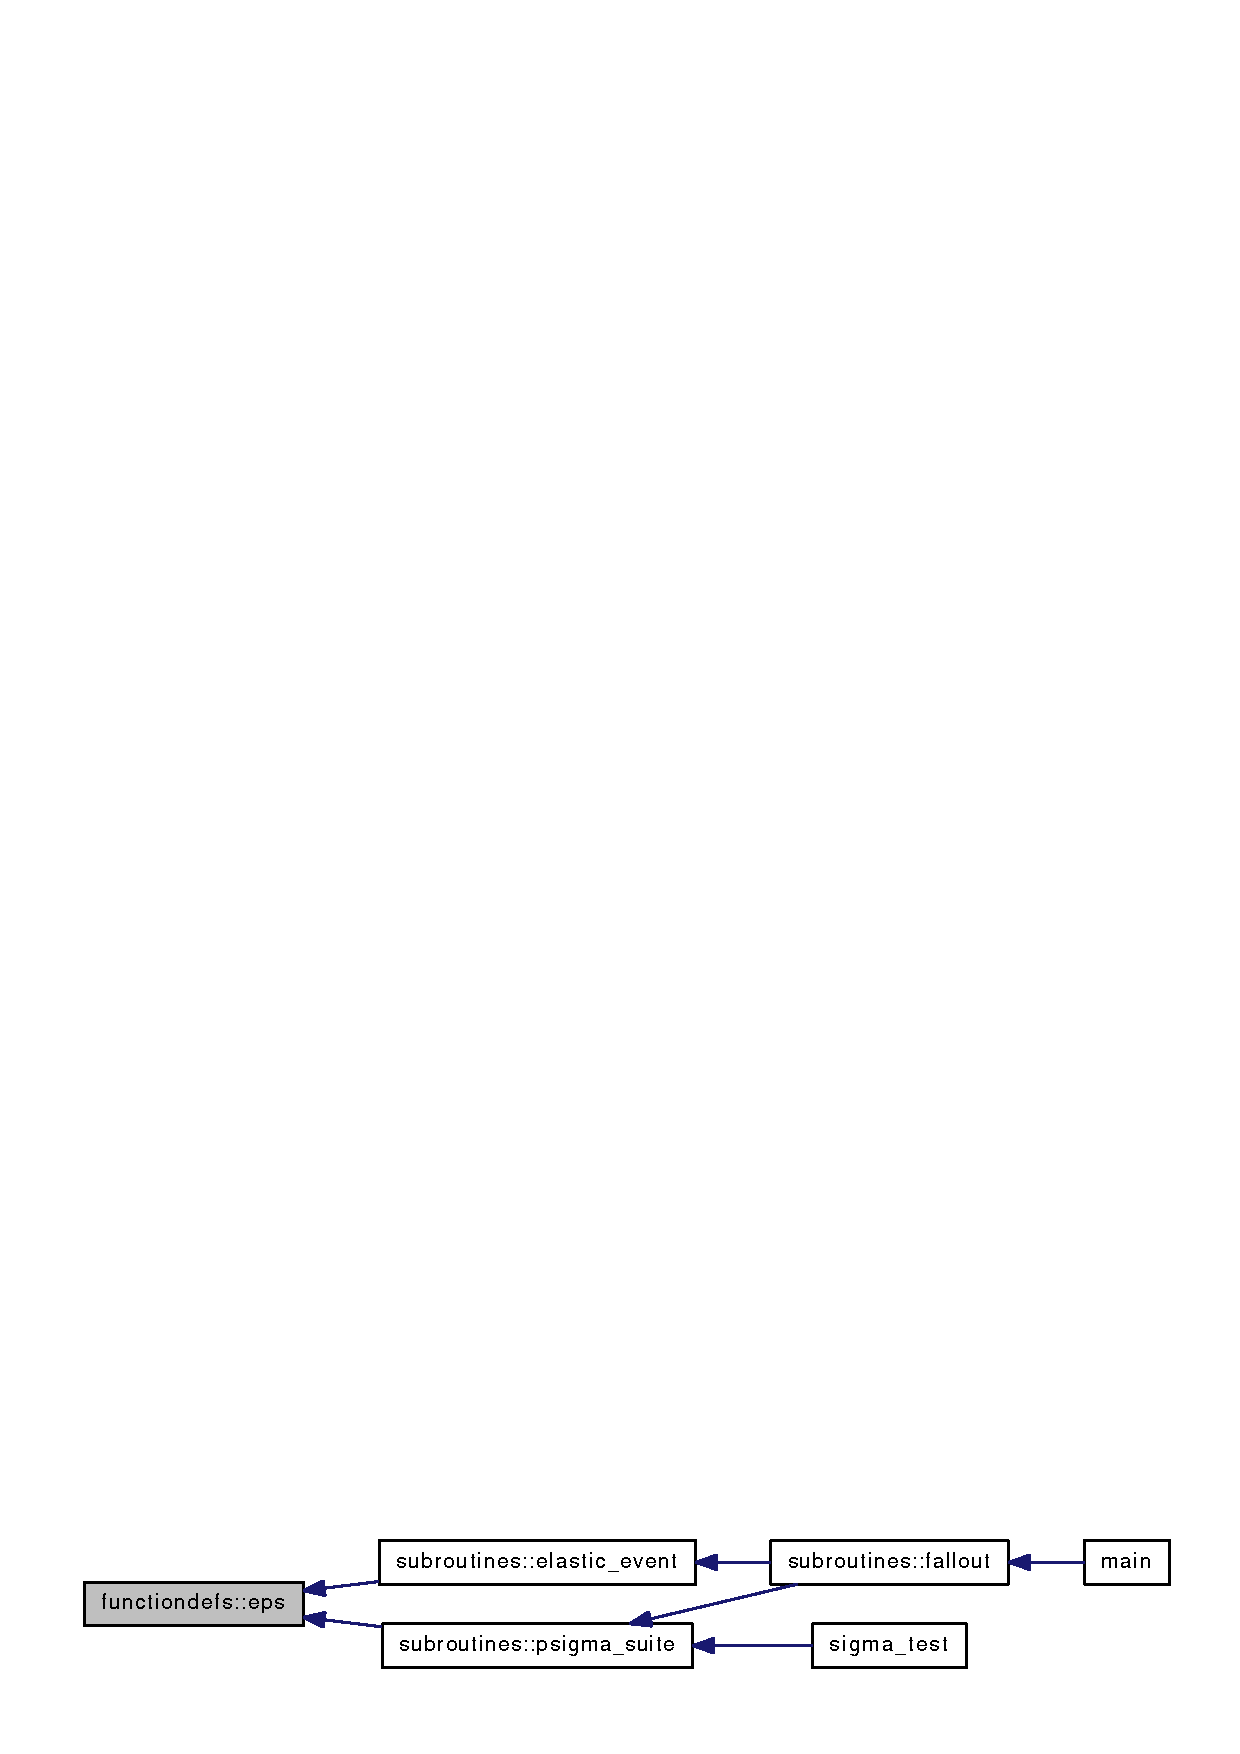
\includegraphics[width=283pt]{namespacefunctiondefs_ac20c2b09d0408eb23b226af7f8f7361a_icgraph}
\end{center}
\end{figure}
\hypertarget{namespacefunctiondefs_adae12a3980d4e2bd5fe6277c91988474}{
\index{functiondefs@{functiondefs}!gamma\_\-gs@{gamma\_\-gs}}
\index{gamma\_\-gs@{gamma\_\-gs}!functiondefs@{functiondefs}}
\subsubsection[{gamma\_\-gs}]{\setlength{\rightskip}{0pt plus 5cm}DOUBLE PRECISION functiondefs::gamma\_\-gs (DOUBLE PRECISION,intent(in) {\em energy}, \/  DOUBLE PRECISION,intent(in) {\em gamma\_\-s}, \/  DOUBLE PRECISION,intent(in) {\em gamma\_\-b})}}
\label{namespacefunctiondefs_adae12a3980d4e2bd5fe6277c91988474}


Definition at line 89 of file functiondefs.f90.

Referenced by subroutines::esigma\_\-suite().

Here is the caller graph for this function:\nopagebreak
\begin{figure}[H]
\begin{center}
\leavevmode
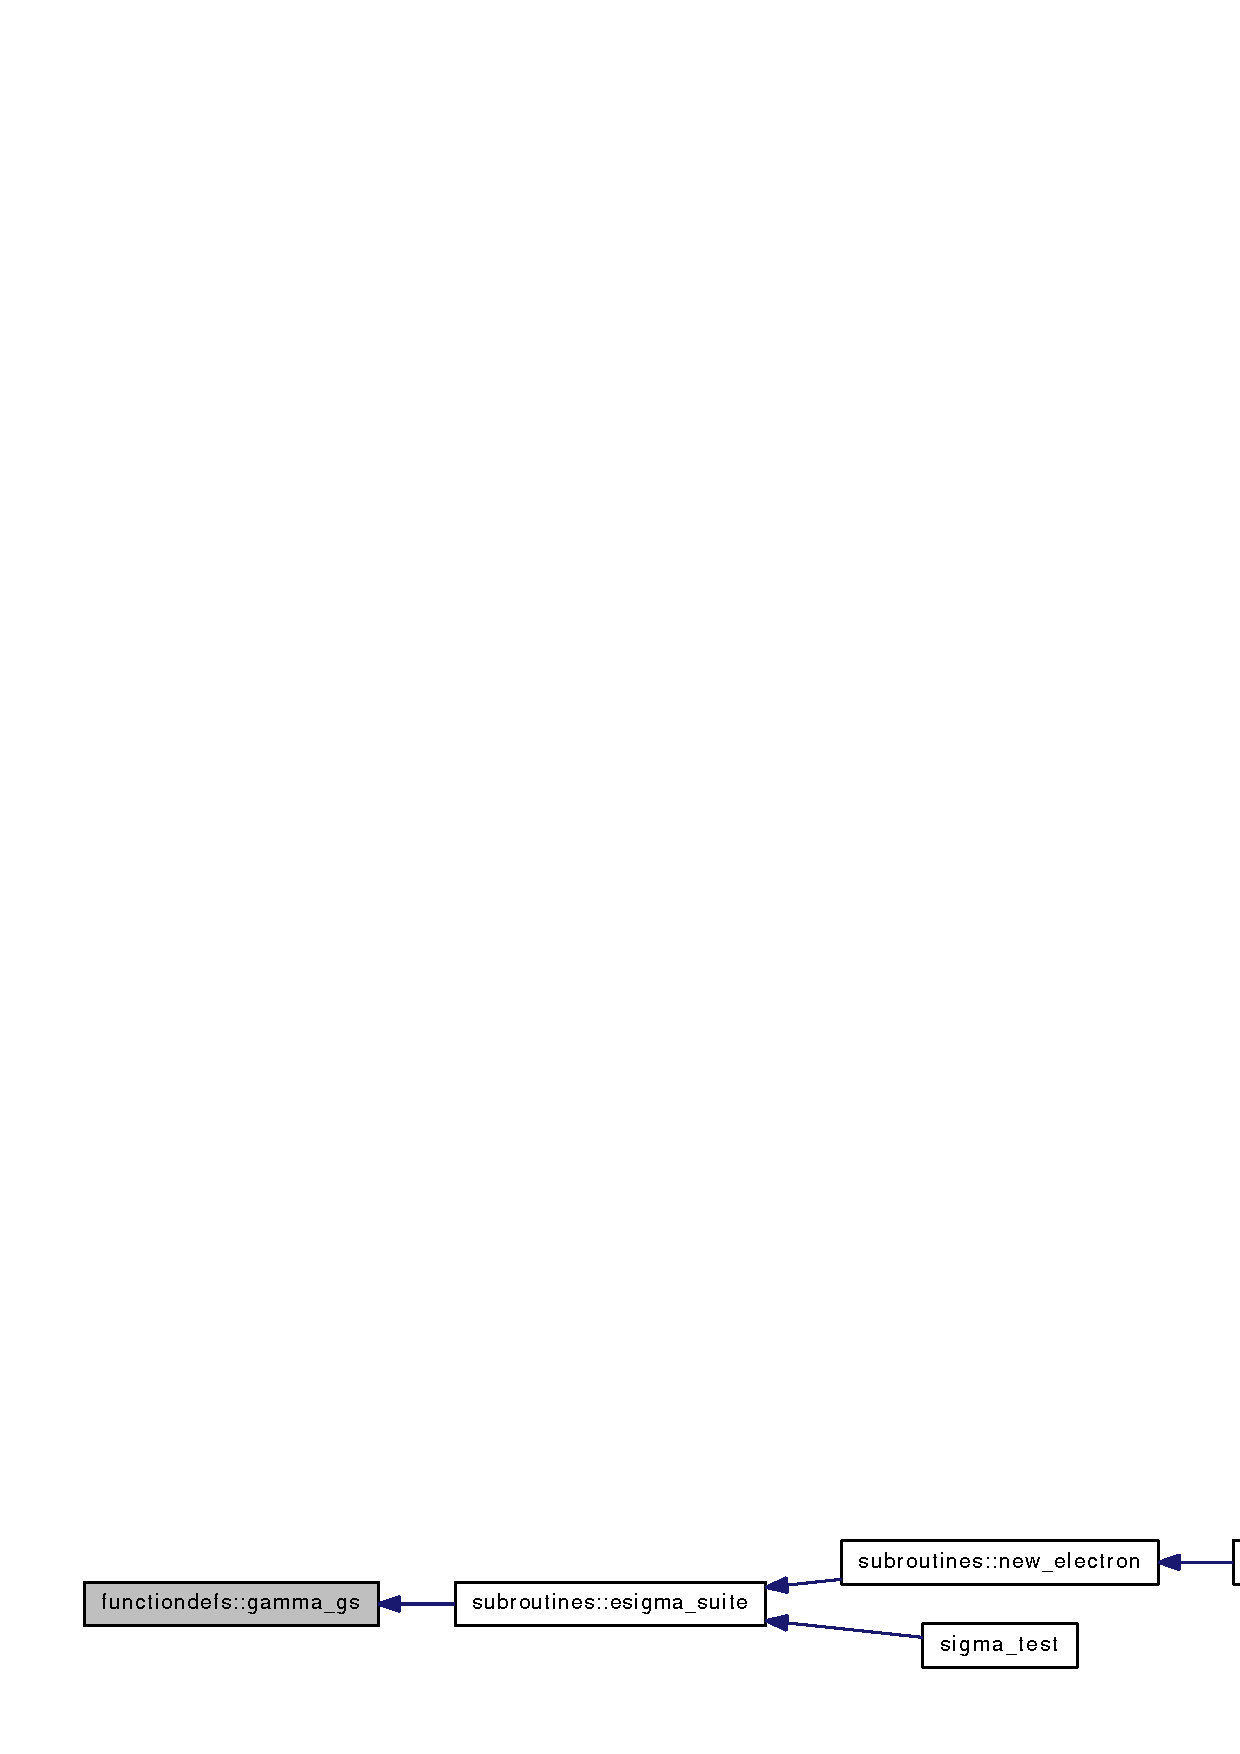
\includegraphics[width=394pt]{namespacefunctiondefs_adae12a3980d4e2bd5fe6277c91988474_icgraph}
\end{center}
\end{figure}
\hypertarget{namespacefunctiondefs_ad75756612cb12ba4983414cdc520f6a1}{
\index{functiondefs@{functiondefs}!green\_\-mcneal@{green\_\-mcneal}}
\index{green\_\-mcneal@{green\_\-mcneal}!functiondefs@{functiondefs}}
\subsubsection[{green\_\-mcneal}]{\setlength{\rightskip}{0pt plus 5cm}DOUBLE PRECISION functiondefs::green\_\-mcneal (DOUBLE PRECISION,intent(in) {\em energy}, \/  DOUBLE PRECISION,intent(in) {\em a}, \/  DOUBLE PRECISION,intent(in) {\em j}, \/  DOUBLE PRECISION,intent(in) {\em nu}, \/  DOUBLE PRECISION,intent(in) {\em omega}, \/  DOUBLE PRECISION,intent(in) {\em z}, \/  DOUBLE PRECISION,intent(in) {\em i})}}
\label{namespacefunctiondefs_ad75756612cb12ba4983414cdc520f6a1}


Definition at line 15 of file functiondefs.f90.

Referenced by subroutines::esigma\_\-suite(), and subroutines::psigma\_\-suite().

Here is the caller graph for this function:\nopagebreak
\begin{figure}[H]
\begin{center}
\leavevmode
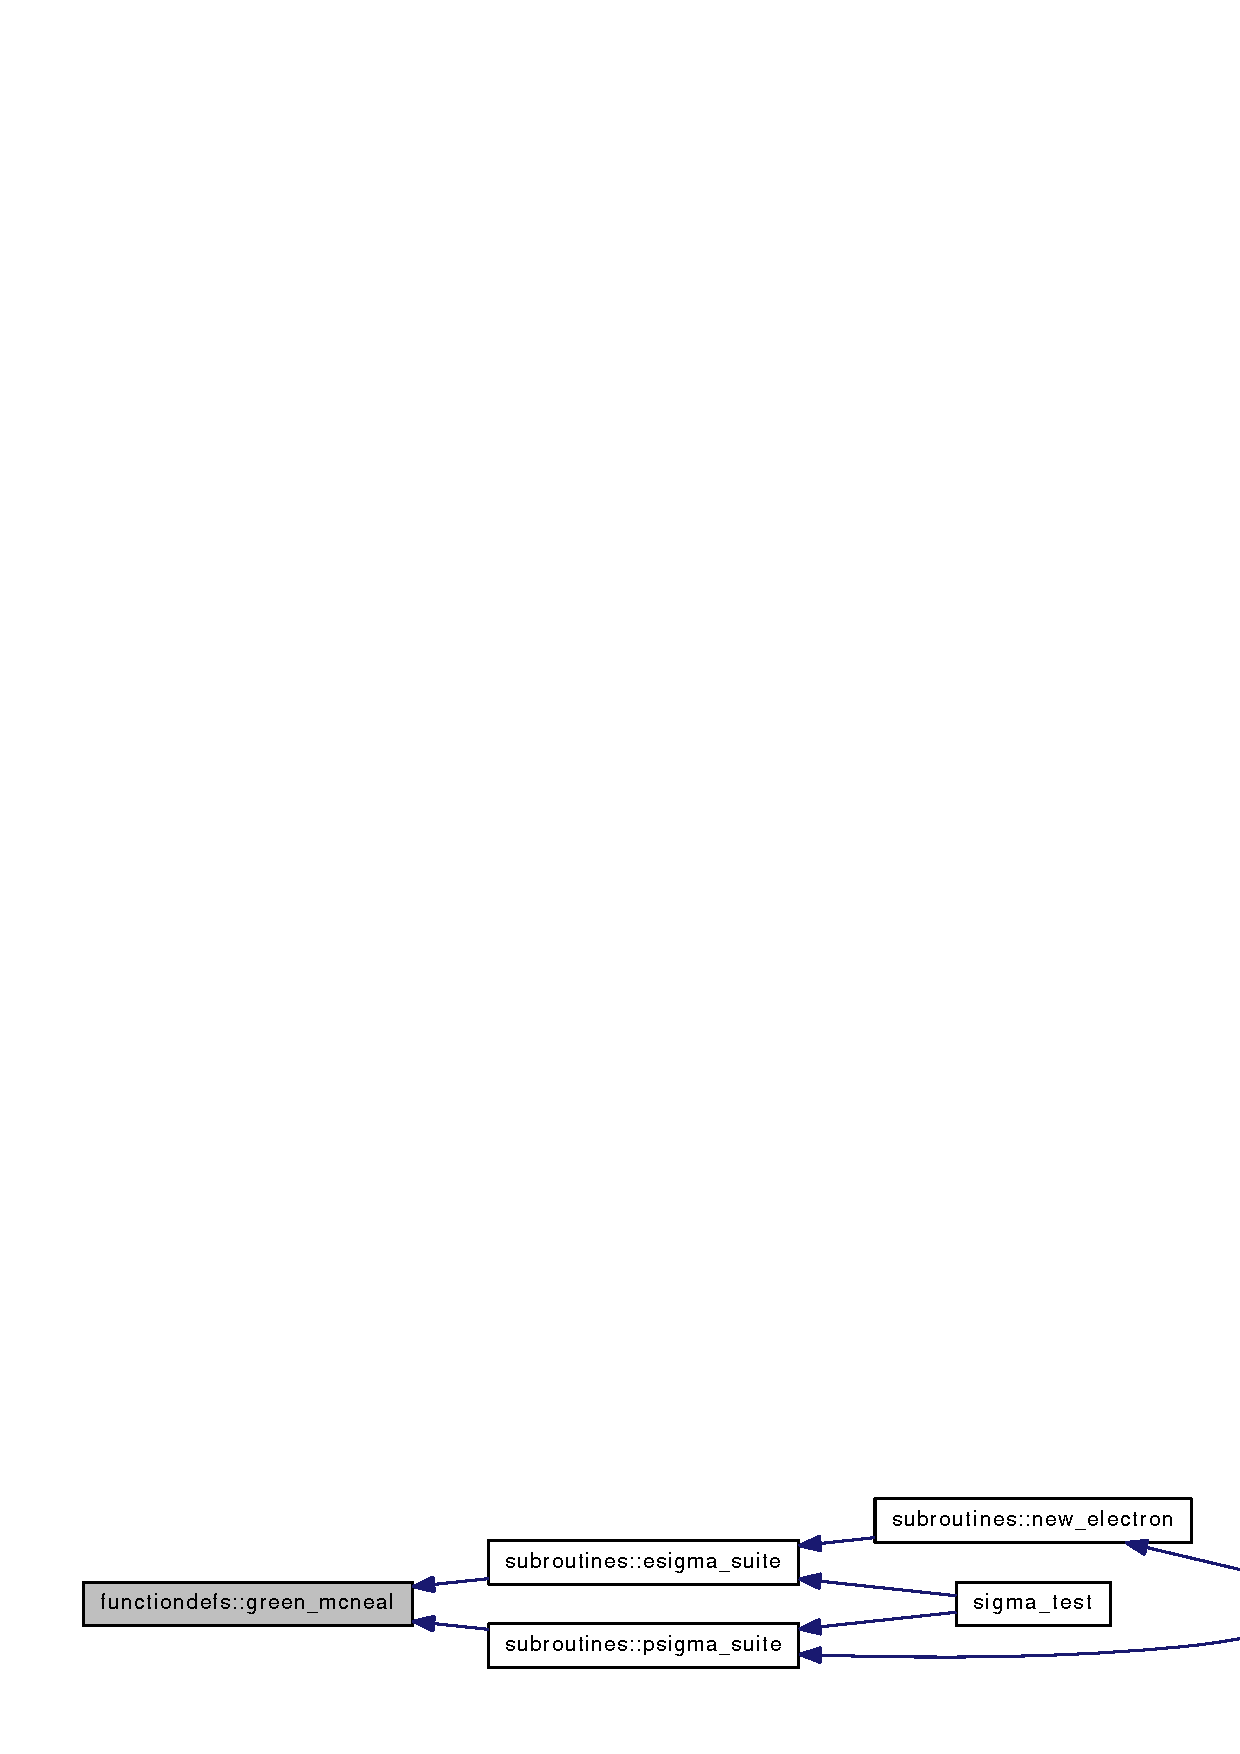
\includegraphics[width=402pt]{namespacefunctiondefs_ad75756612cb12ba4983414cdc520f6a1_icgraph}
\end{center}
\end{figure}
\hypertarget{namespacefunctiondefs_a64cc5970914d70f20e127be3722f11bb}{
\index{functiondefs@{functiondefs}!green\_\-sawada@{green\_\-sawada}}
\index{green\_\-sawada@{green\_\-sawada}!functiondefs@{functiondefs}}
\subsubsection[{green\_\-sawada}]{\setlength{\rightskip}{0pt plus 5cm}DOUBLE PRECISION functiondefs::green\_\-sawada (DOUBLE PRECISION,intent(in) {\em a}, \/  DOUBLE PRECISION,intent(in) {\em gamma\_\-fac}, \/  DOUBLE PRECISION,intent(in) {\em t\_\-max}, \/  DOUBLE PRECISION,intent(in) {\em t\_\-0})}}
\label{namespacefunctiondefs_a64cc5970914d70f20e127be3722f11bb}


Definition at line 171 of file functiondefs.f90.

Referenced by subroutines::esigma\_\-suite().

Here is the caller graph for this function:\nopagebreak
\begin{figure}[H]
\begin{center}
\leavevmode
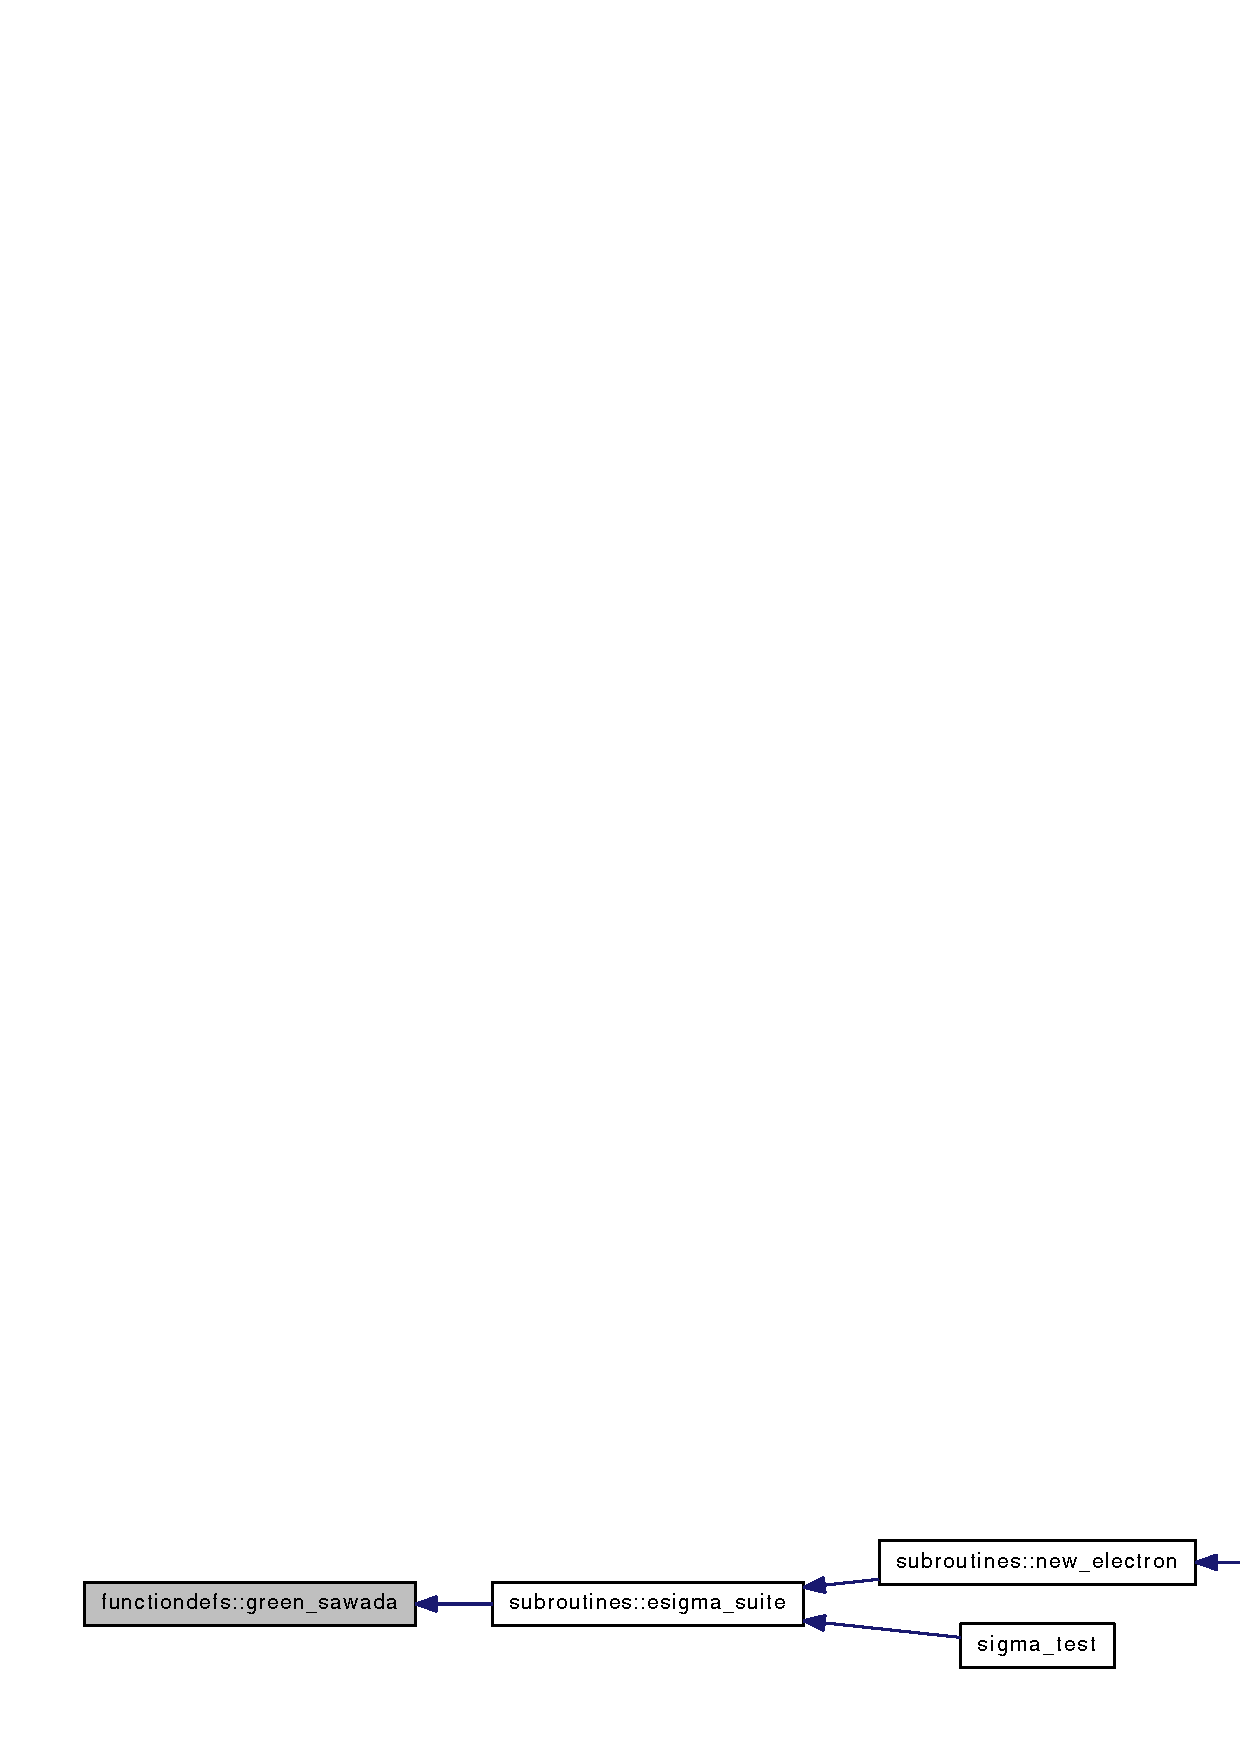
\includegraphics[width=403pt]{namespacefunctiondefs_a64cc5970914d70f20e127be3722f11bb_icgraph}
\end{center}
\end{figure}
\hypertarget{namespacefunctiondefs_a7a31d88fad502937338eafac9a574fec}{
\index{functiondefs@{functiondefs}!greendutta@{greendutta}}
\index{greendutta@{greendutta}!functiondefs@{functiondefs}}
\subsubsection[{greendutta}]{\setlength{\rightskip}{0pt plus 5cm}DOUBLE PRECISION functiondefs::greendutta (DOUBLE PRECISION,intent(in) {\em energy}, \/  DOUBLE PRECISION,intent(in) {\em w}, \/  DOUBLE PRECISION,intent(in) {\em f}, \/  DOUBLE PRECISION,intent(in) {\em o}, \/  DOUBLE PRECISION,intent(in) {\em a}, \/  DOUBLE PRECISION,intent(in) {\em b})}}
\label{namespacefunctiondefs_a7a31d88fad502937338eafac9a574fec}


Definition at line 587 of file functiondefs.f90.

References parameters::Q0.\hypertarget{namespacefunctiondefs_abeba54805575687a8d1db47decf4790e}{
\index{functiondefs@{functiondefs}!lab\_\-theta@{lab\_\-theta}}
\index{lab\_\-theta@{lab\_\-theta}!functiondefs@{functiondefs}}
\subsubsection[{lab\_\-theta}]{\setlength{\rightskip}{0pt plus 5cm}DOUBLE PRECISION functiondefs::lab\_\-theta (DOUBLE PRECISION,intent(in) {\em cmtheta}, \/  DOUBLE PRECISION,intent(in) {\em m1}, \/  DOUBLE PRECISION,intent(in) {\em m2})}}
\label{namespacefunctiondefs_abeba54805575687a8d1db47decf4790e}


Definition at line 458 of file functiondefs.f90.

Referenced by subroutines::elastic\_\-event().

Here is the caller graph for this function:\nopagebreak
\begin{figure}[H]
\begin{center}
\leavevmode
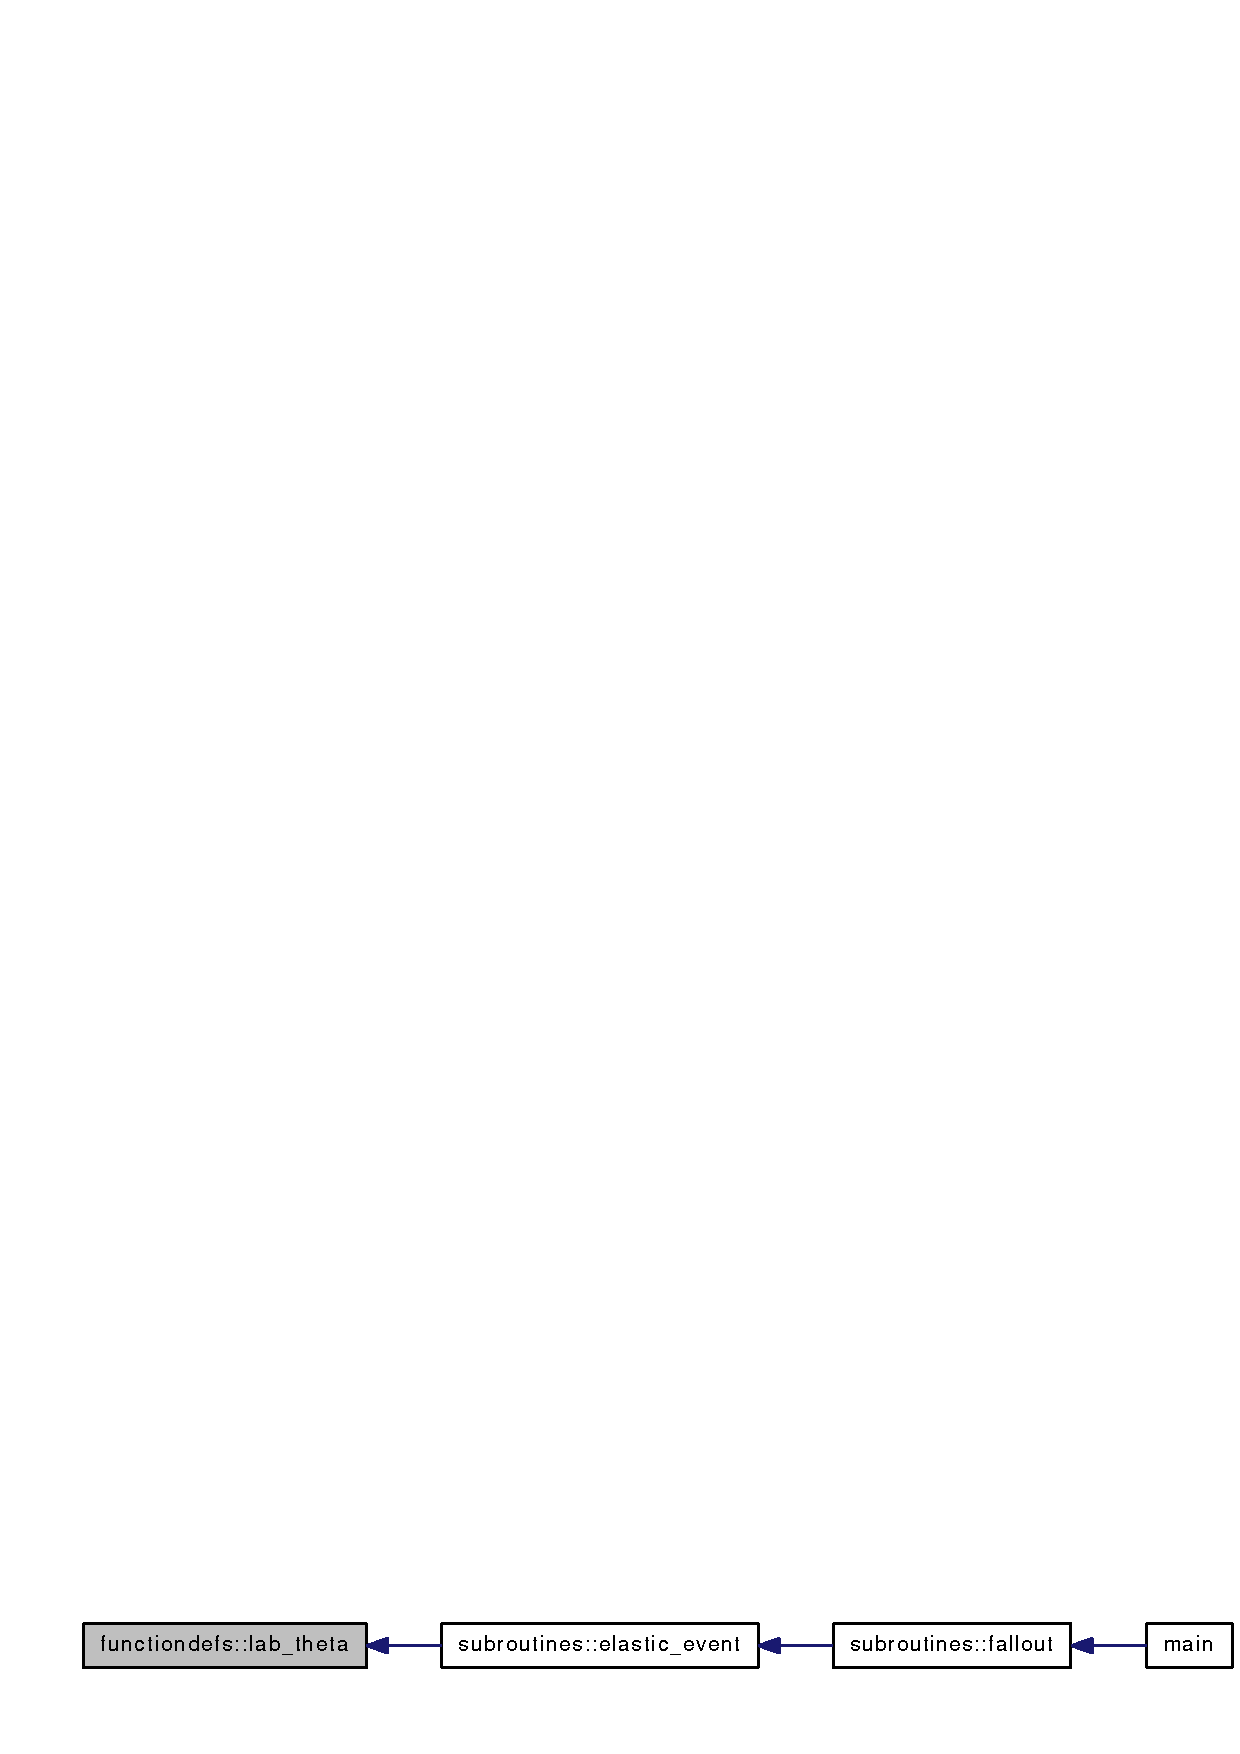
\includegraphics[width=298pt]{namespacefunctiondefs_abeba54805575687a8d1db47decf4790e_icgraph}
\end{center}
\end{figure}
\hypertarget{namespacefunctiondefs_a93c18b11591055e1e1275c6dc7b2ab26}{
\index{functiondefs@{functiondefs}!magic@{magic}}
\index{magic@{magic}!functiondefs@{functiondefs}}
\subsubsection[{magic}]{\setlength{\rightskip}{0pt plus 5cm}subroutine functiondefs::magic (DOUBLE PRECISION,intent(in) {\em eps}, \/  DOUBLE PRECISION,intent(in) {\em b}, \/  DOUBLE PRECISION,intent(out) {\em c2}, \/  DOUBLE PRECISION,intent(out) {\em s2}, \/  DOUBLE PRECISION,intent(out) {\em theta})}}
\label{namespacefunctiondefs_a93c18b11591055e1e1275c6dc7b2ab26}


Definition at line 240 of file functiondefs.f90.

Referenced by subroutines::elastic\_\-event().

Here is the caller graph for this function:\nopagebreak
\begin{figure}[H]
\begin{center}
\leavevmode
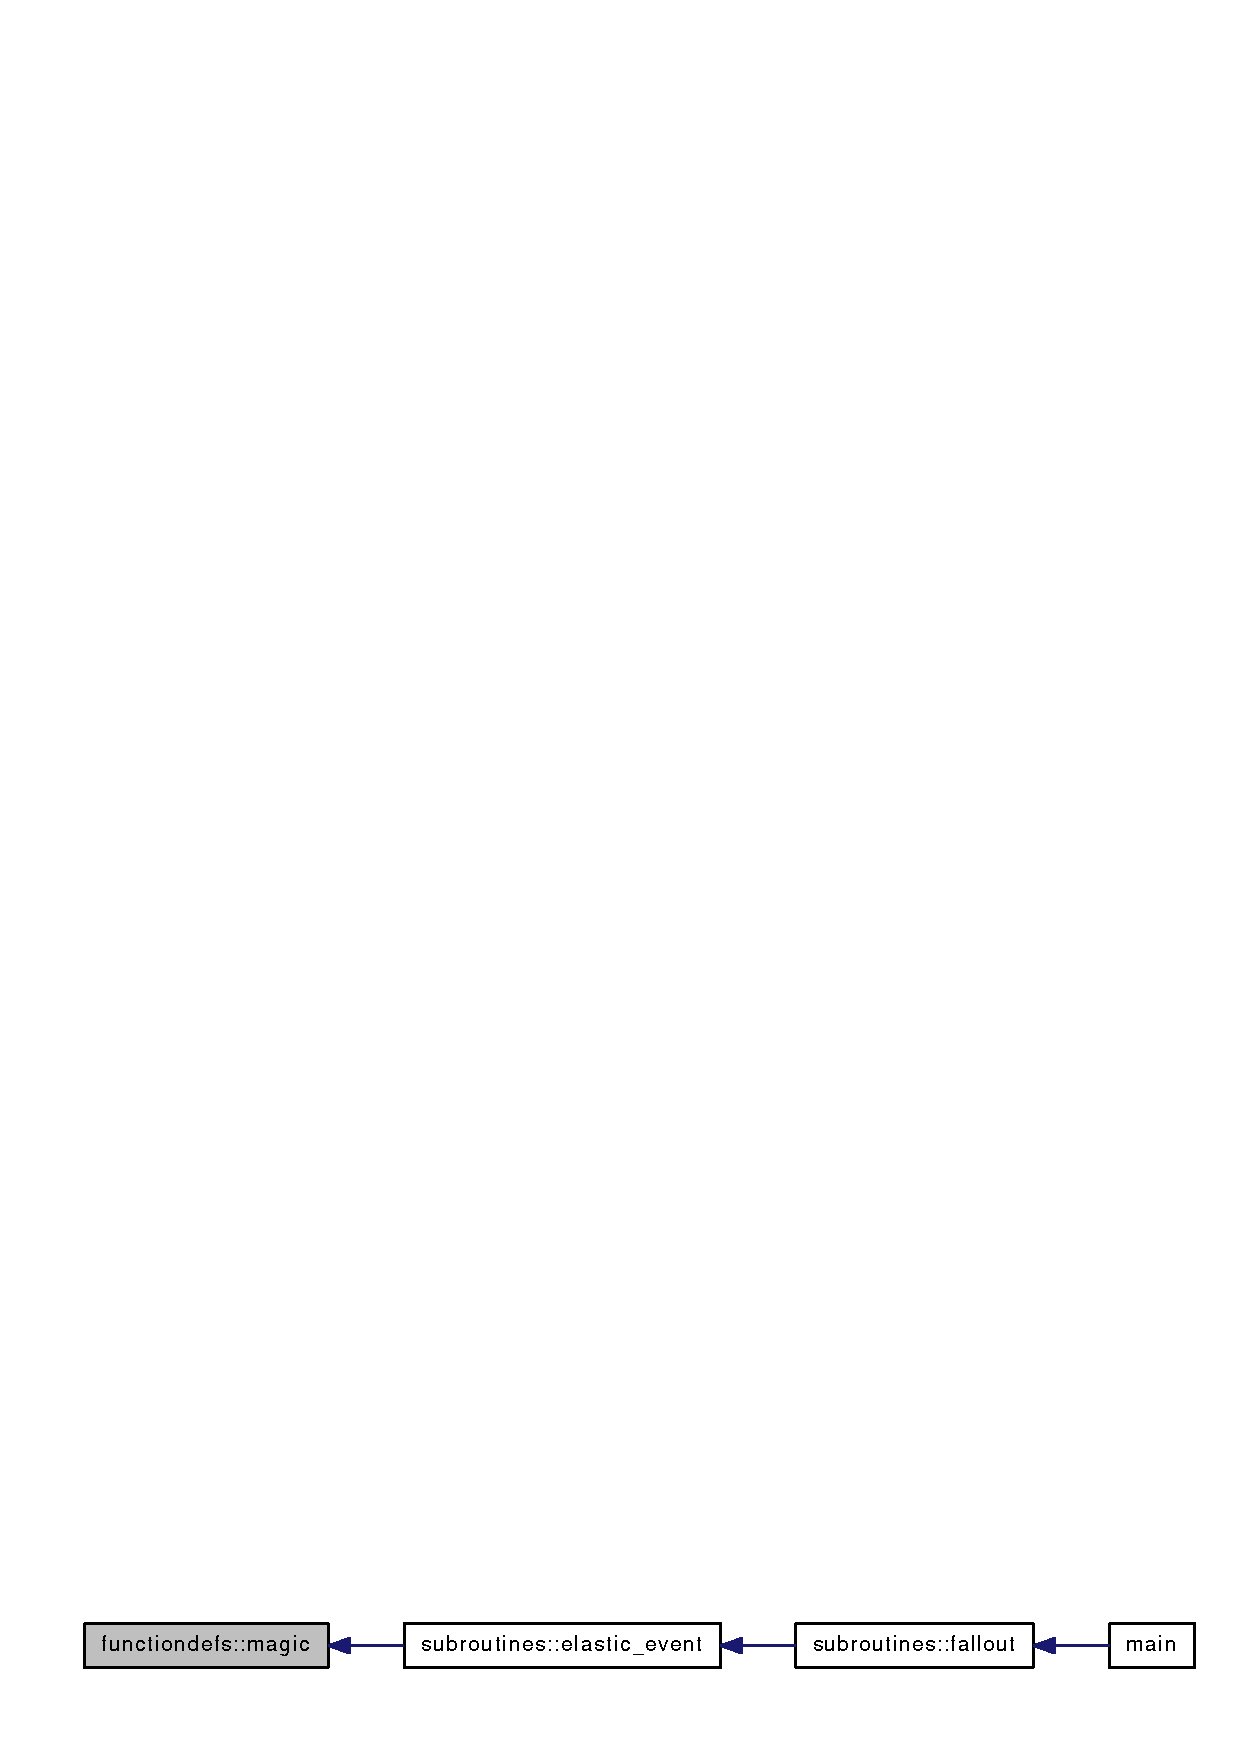
\includegraphics[width=289pt]{namespacefunctiondefs_a93c18b11591055e1e1275c6dc7b2ab26_icgraph}
\end{center}
\end{figure}
\hypertarget{namespacefunctiondefs_aa92057c8da0a7ce374166fed435ea54f}{
\index{functiondefs@{functiondefs}!mass\_\-fac@{mass\_\-fac}}
\index{mass\_\-fac@{mass\_\-fac}!functiondefs@{functiondefs}}
\subsubsection[{mass\_\-fac}]{\setlength{\rightskip}{0pt plus 5cm}DOUBLE PRECISION functiondefs::mass\_\-fac (DOUBLE PRECISION,intent(in) {\em m1}, \/  DOUBLE PRECISION,intent(in) {\em m2})}}
\label{namespacefunctiondefs_aa92057c8da0a7ce374166fed435ea54f}


Definition at line 409 of file functiondefs.f90.

Referenced by subroutines::elastic\_\-event(), and subroutines::psigma\_\-suite().

Here is the caller graph for this function:\nopagebreak
\begin{figure}[H]
\begin{center}
\leavevmode
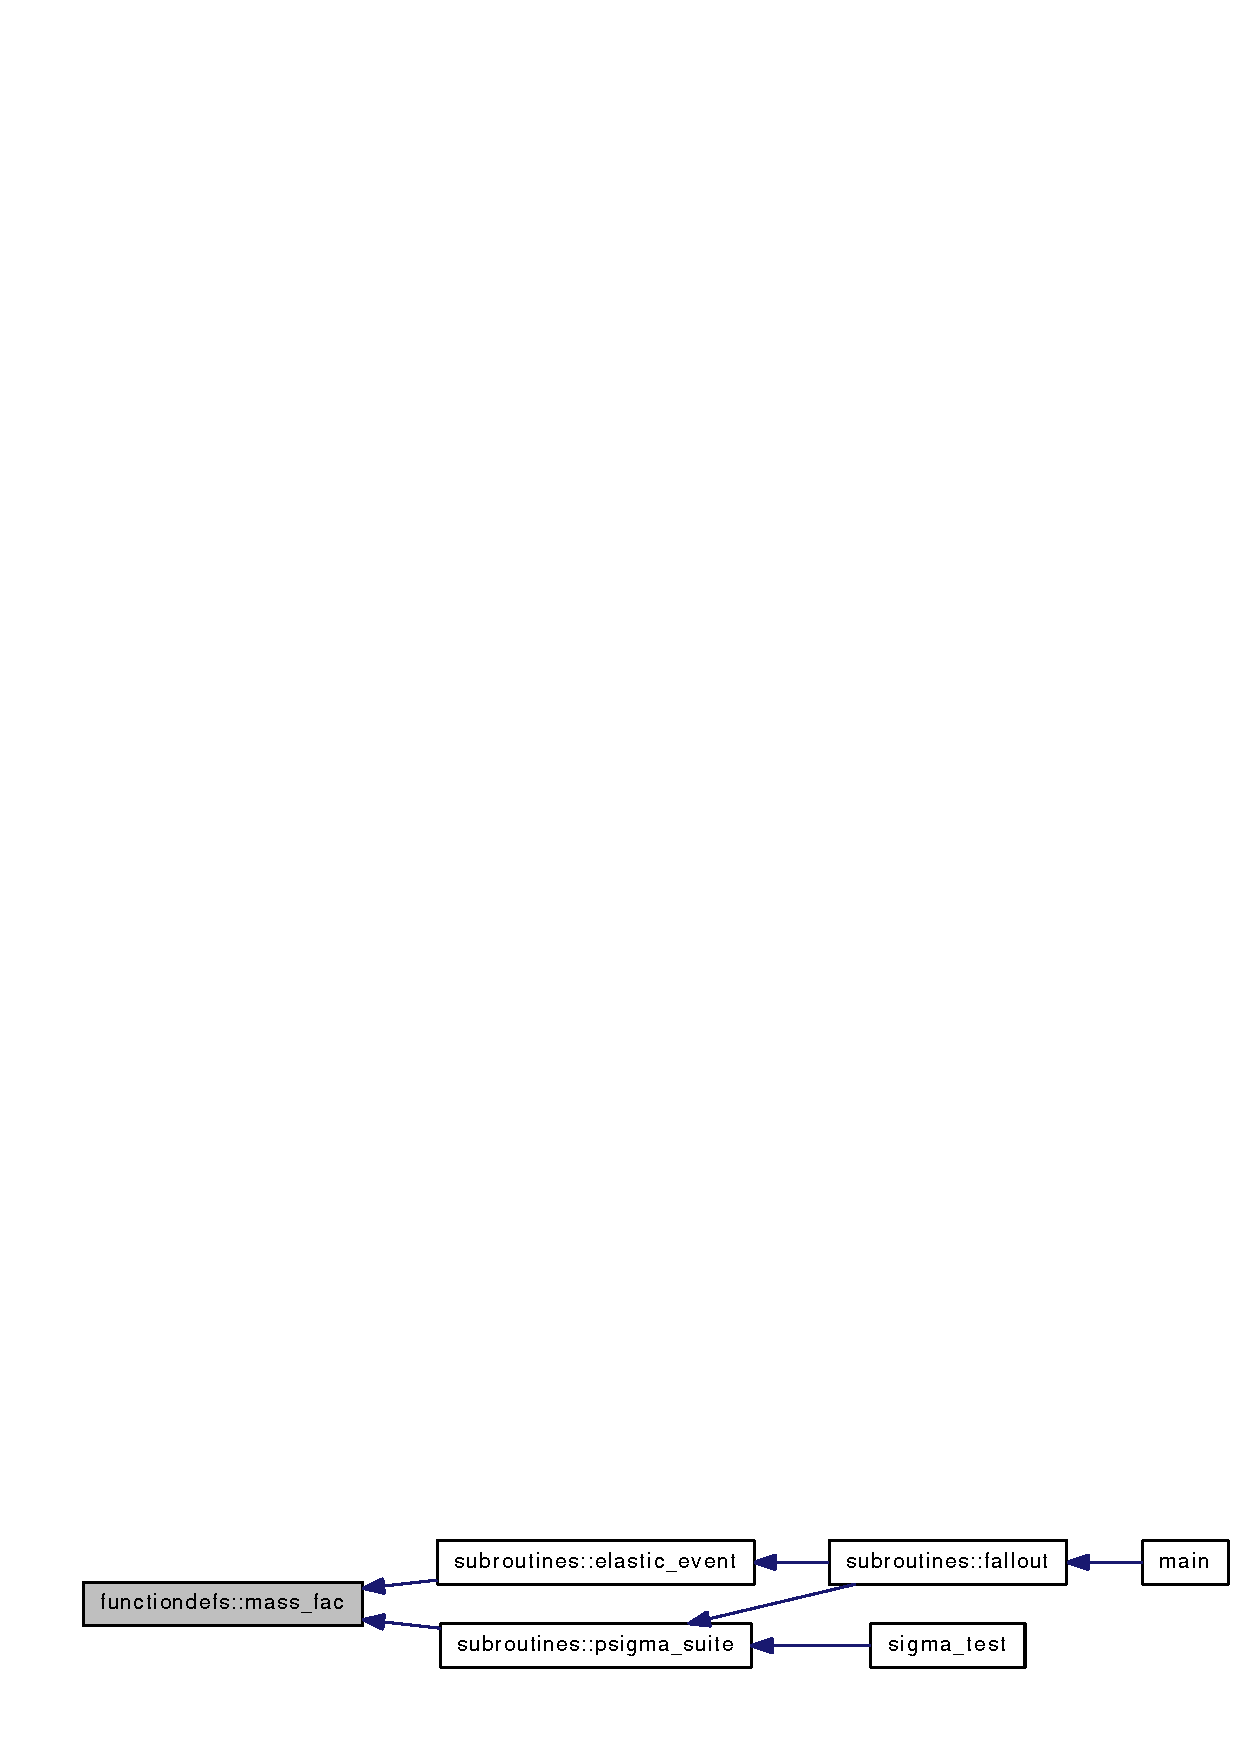
\includegraphics[width=297pt]{namespacefunctiondefs_aa92057c8da0a7ce374166fed435ea54f_icgraph}
\end{center}
\end{figure}
\hypertarget{namespacefunctiondefs_abb5f2d51b3f8b637e0d17ad8c21db948}{
\index{functiondefs@{functiondefs}!ne\_\-mg@{ne\_\-mg}}
\index{ne\_\-mg@{ne\_\-mg}!functiondefs@{functiondefs}}
\subsubsection[{ne\_\-mg}]{\setlength{\rightskip}{0pt plus 5cm}REAL functiondefs::ne\_\-mg (REAL,intent(in) {\em gamma\_\-fac}, \/  REAL,intent(in) {\em t\_\-max}, \/  REAL,intent(in) {\em t\_\-0})}}
\label{namespacefunctiondefs_abb5f2d51b3f8b637e0d17ad8c21db948}


Definition at line 209 of file functiondefs.f90.\hypertarget{namespacefunctiondefs_ae52b03b9e83dd8f46fd7532fb105850b}{
\index{functiondefs@{functiondefs}!pelsig@{pelsig}}
\index{pelsig@{pelsig}!functiondefs@{functiondefs}}
\subsubsection[{pelsig}]{\setlength{\rightskip}{0pt plus 5cm}DOUBLE PRECISION functiondefs::pelsig (DOUBLE PRECISION,intent(in) {\em energy}, \/  DOUBLE PRECISION,intent(in) {\em sne}, \/  DOUBLE PRECISION,intent(in) {\em mf})}}
\label{namespacefunctiondefs_ae52b03b9e83dd8f46fd7532fb105850b}


Definition at line 562 of file functiondefs.f90.

Referenced by subroutines::psigma\_\-suite().

Here is the caller graph for this function:\nopagebreak
\begin{figure}[H]
\begin{center}
\leavevmode
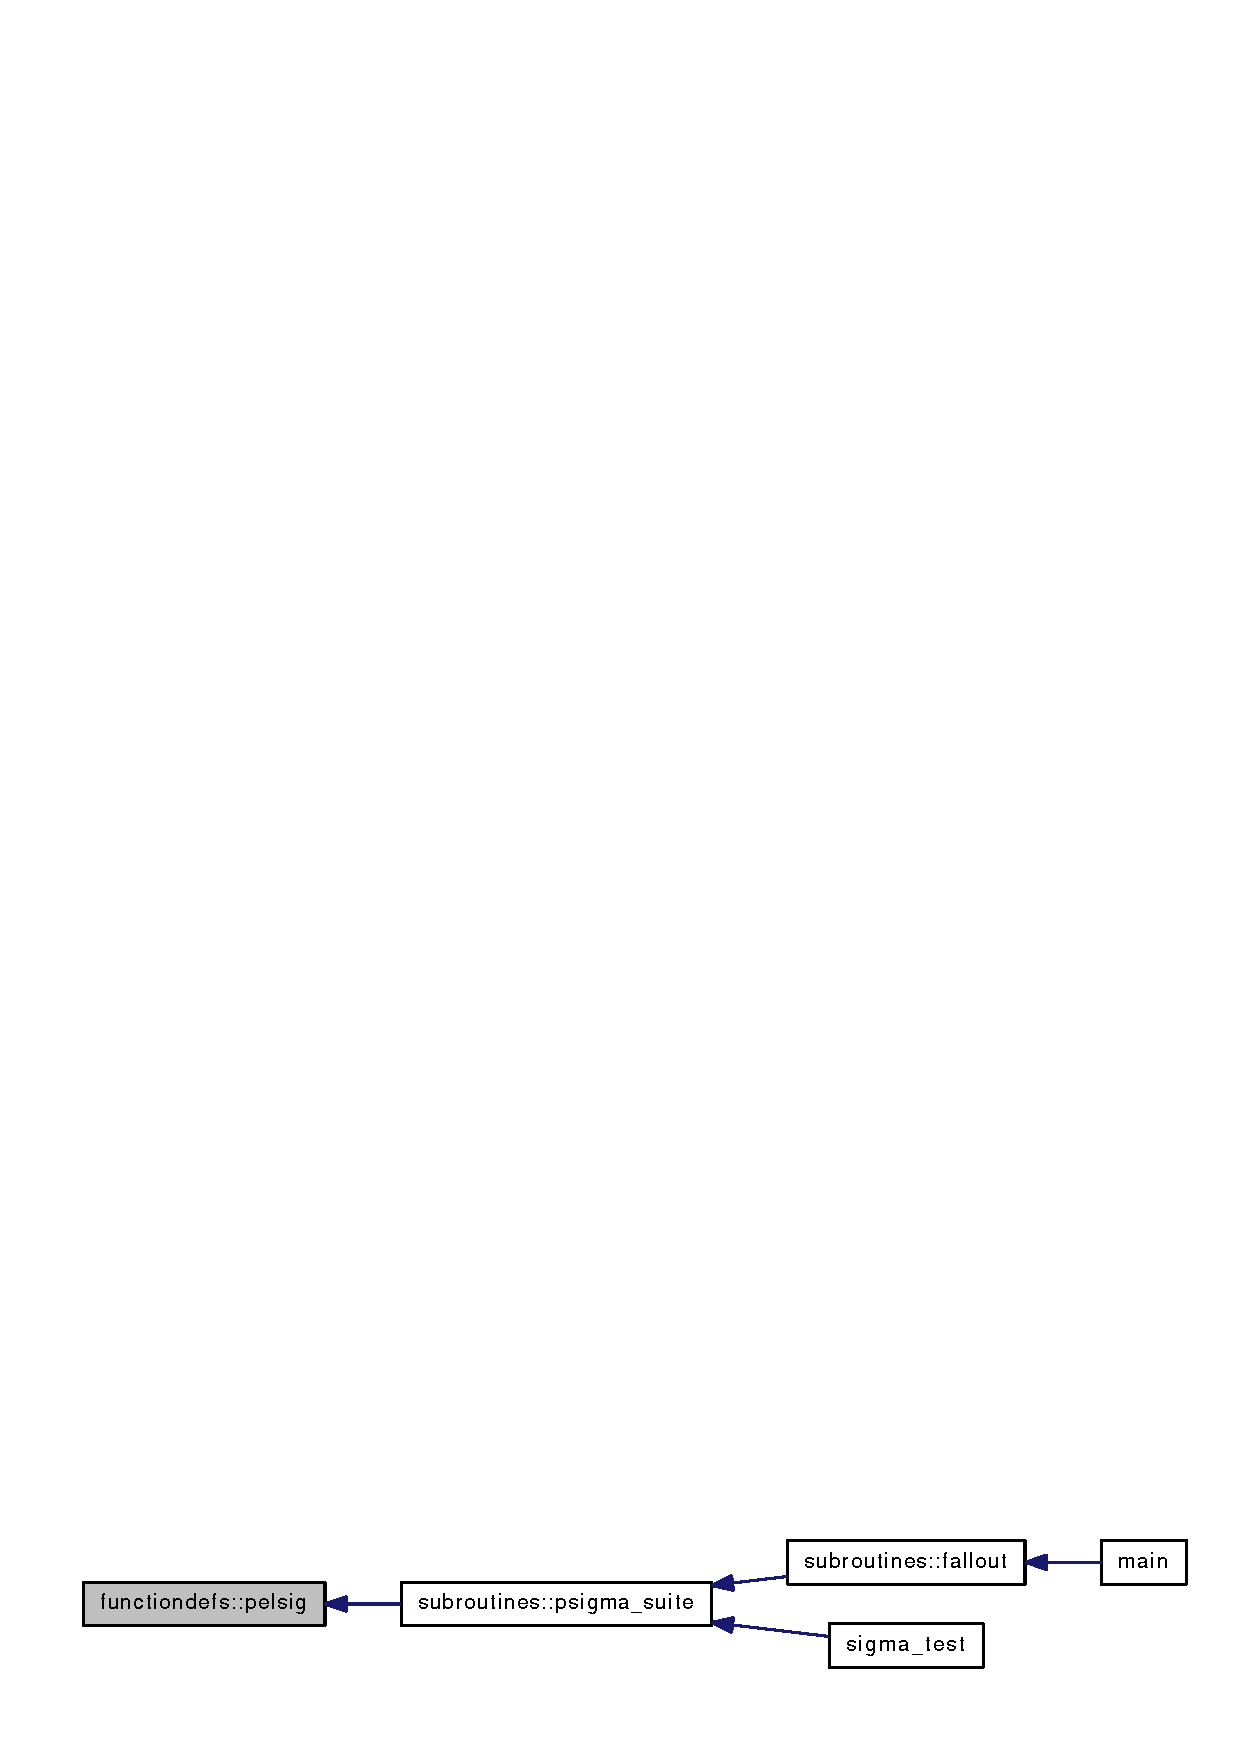
\includegraphics[width=287pt]{namespacefunctiondefs_ae52b03b9e83dd8f46fd7532fb105850b_icgraph}
\end{center}
\end{figure}
\hypertarget{namespacefunctiondefs_a5486e5e48a1c871c2ec9d5bc03406ea5}{
\index{functiondefs@{functiondefs}!pjgsigma@{pjgsigma}}
\index{pjgsigma@{pjgsigma}!functiondefs@{functiondefs}}
\subsubsection[{pjgsigma}]{\setlength{\rightskip}{0pt plus 5cm}DOUBLE PRECISION functiondefs::pjgsigma (DOUBLE PRECISION,intent(in) {\em energy}, \/  DOUBLE PRECISION,intent(in) {\em f}, \/  DOUBLE PRECISION,intent(in) {\em w}, \/  DOUBLE PRECISION,intent(in) {\em c}, \/  DOUBLE PRECISION,intent(in) {\em a}, \/  DOUBLE PRECISION,intent(in) {\em b})}}
\label{namespacefunctiondefs_a5486e5e48a1c871c2ec9d5bc03406ea5}


Definition at line 630 of file functiondefs.f90.

References parameters::EBASE, and parameters::Q0.

Referenced by subroutines::esigma\_\-suite().

Here is the caller graph for this function:\nopagebreak
\begin{figure}[H]
\begin{center}
\leavevmode
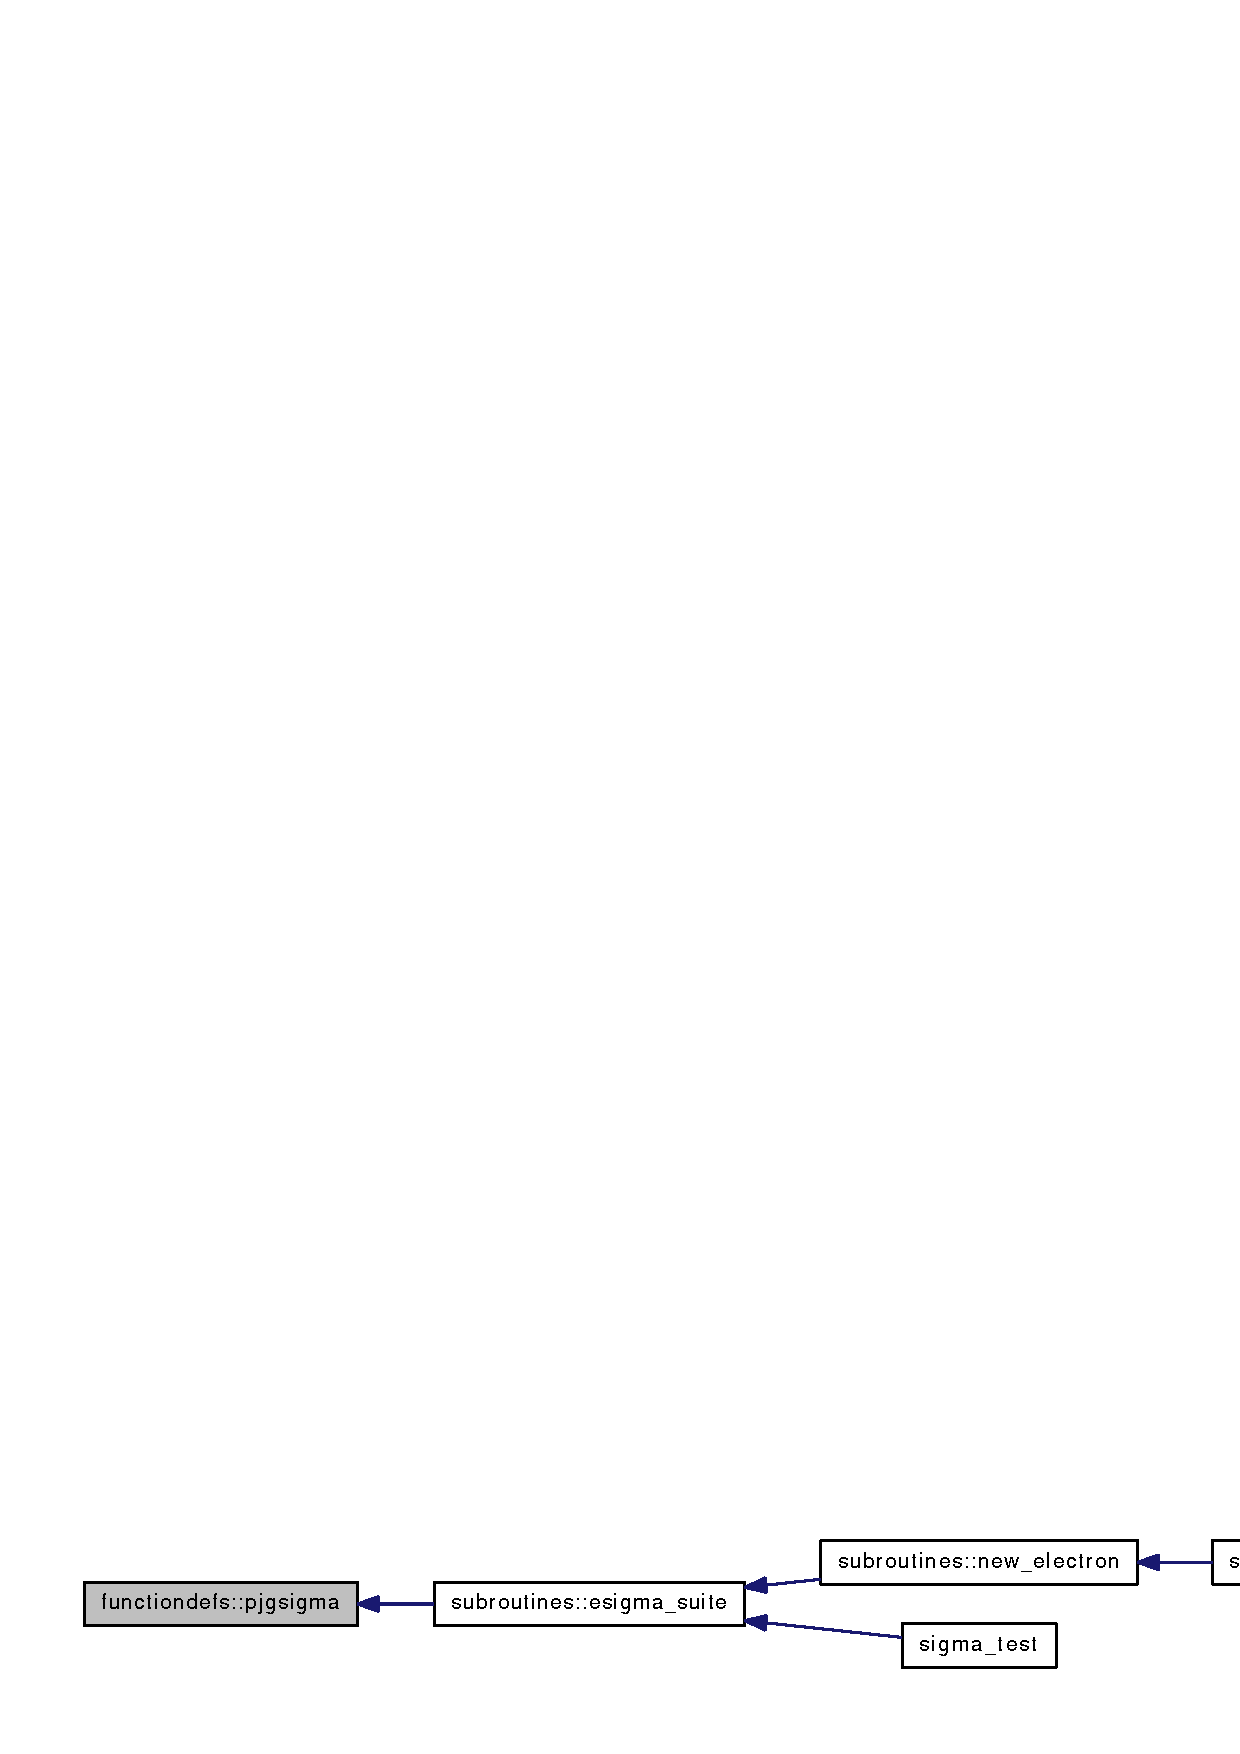
\includegraphics[width=389pt]{namespacefunctiondefs_a5486e5e48a1c871c2ec9d5bc03406ea5_icgraph}
\end{center}
\end{figure}
\hypertarget{namespacefunctiondefs_a78455979576075ad68feb125604462bc}{
\index{functiondefs@{functiondefs}!sne@{sne}}
\index{sne@{sne}!functiondefs@{functiondefs}}
\subsubsection[{sne}]{\setlength{\rightskip}{0pt plus 5cm}DOUBLE PRECISION functiondefs::sne (DOUBLE PRECISION,intent(in) {\em sneps}, \/  DOUBLE PRECISION,intent(in) {\em z1}, \/  DOUBLE PRECISION,intent(in) {\em z2}, \/  DOUBLE PRECISION,intent(in) {\em m1}, \/  DOUBLE PRECISION,intent(in) {\em m2})}}
\label{namespacefunctiondefs_a78455979576075ad68feb125604462bc}


Definition at line 526 of file functiondefs.f90.

Referenced by subroutines::psigma\_\-suite().

Here is the caller graph for this function:\nopagebreak
\begin{figure}[H]
\begin{center}
\leavevmode
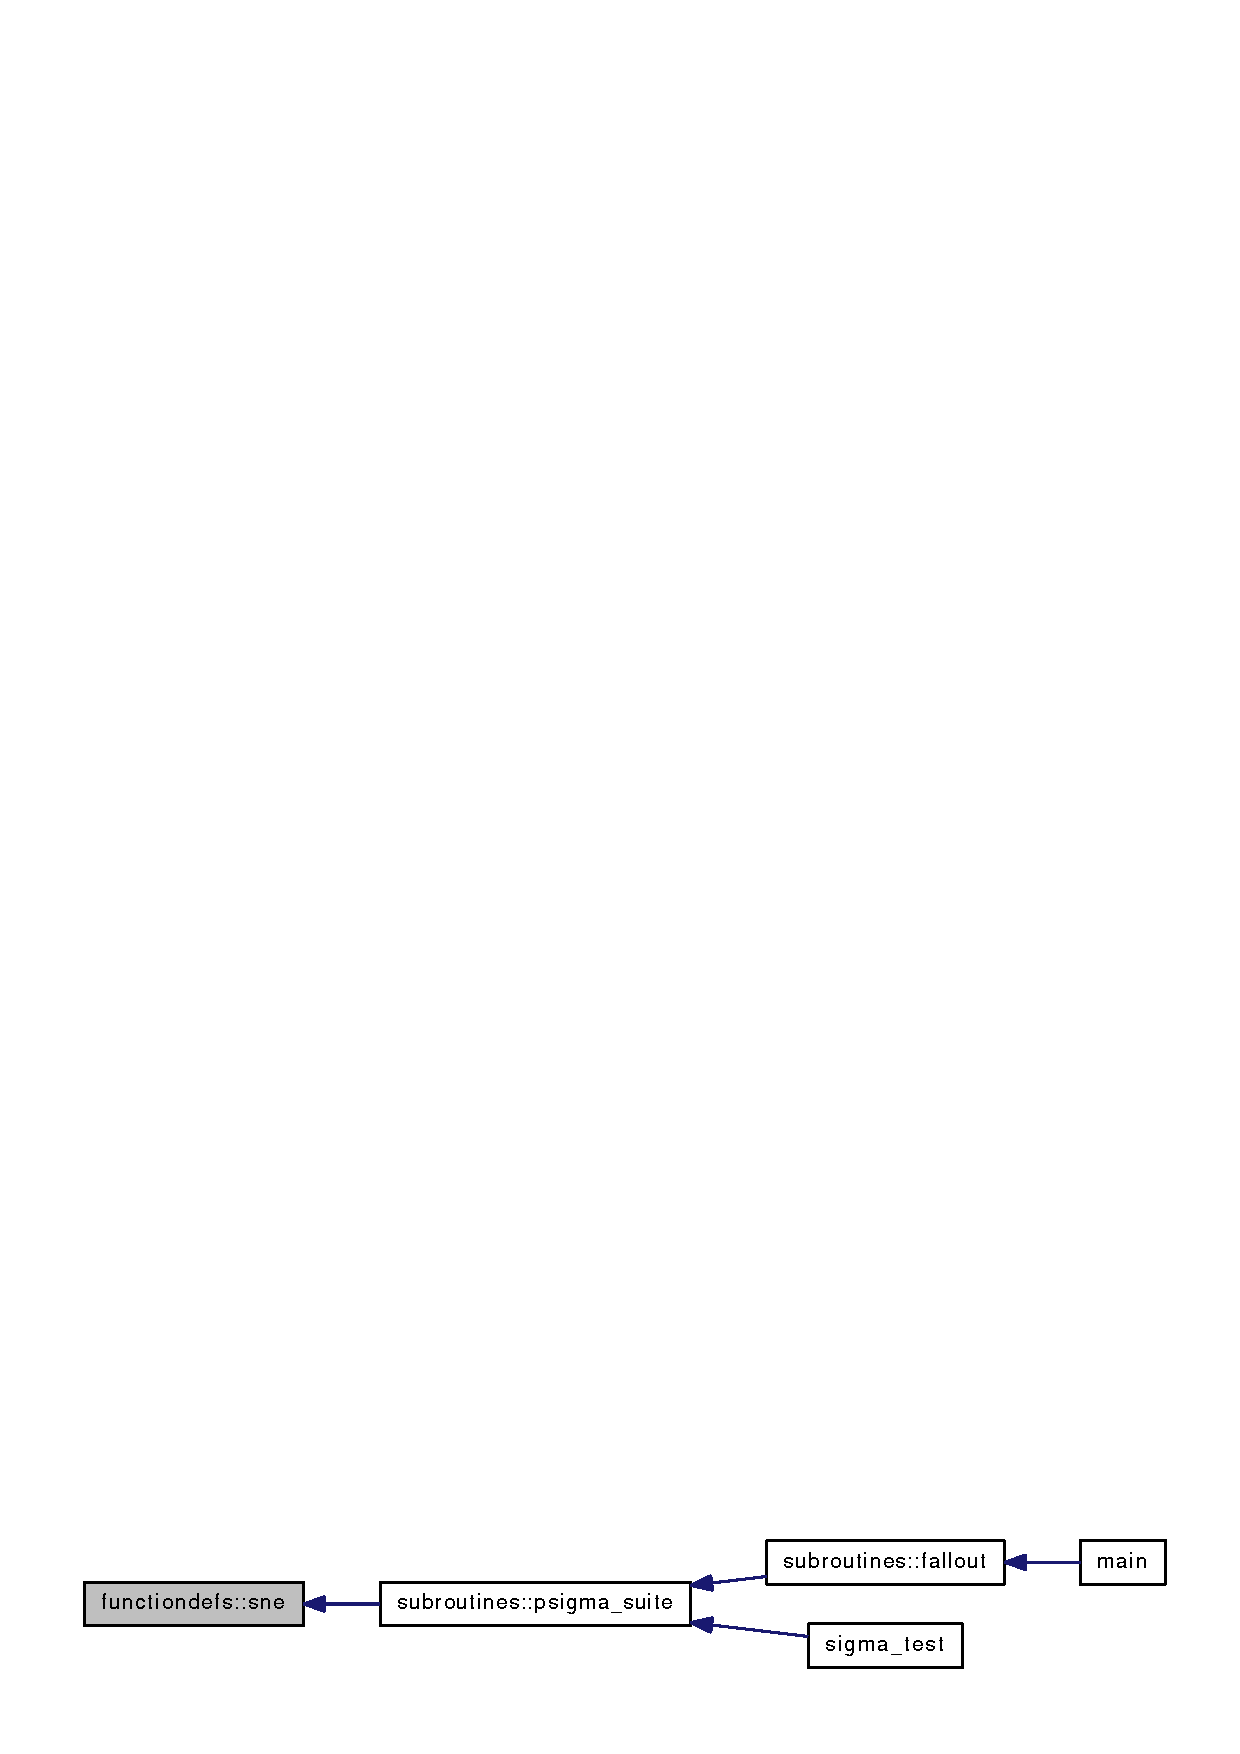
\includegraphics[width=282pt]{namespacefunctiondefs_a78455979576075ad68feb125604462bc_icgraph}
\end{center}
\end{figure}
\hypertarget{namespacefunctiondefs_a80d99fe52a1cb5856694596955d8aeb9}{
\index{functiondefs@{functiondefs}!sneps@{sneps}}
\index{sneps@{sneps}!functiondefs@{functiondefs}}
\subsubsection[{sneps}]{\setlength{\rightskip}{0pt plus 5cm}DOUBLE PRECISION functiondefs::sneps (DOUBLE PRECISION,intent(in) {\em eps})}}
\label{namespacefunctiondefs_a80d99fe52a1cb5856694596955d8aeb9}


Definition at line 487 of file functiondefs.f90.

Referenced by subroutines::psigma\_\-suite().

Here is the caller graph for this function:\nopagebreak
\begin{figure}[H]
\begin{center}
\leavevmode
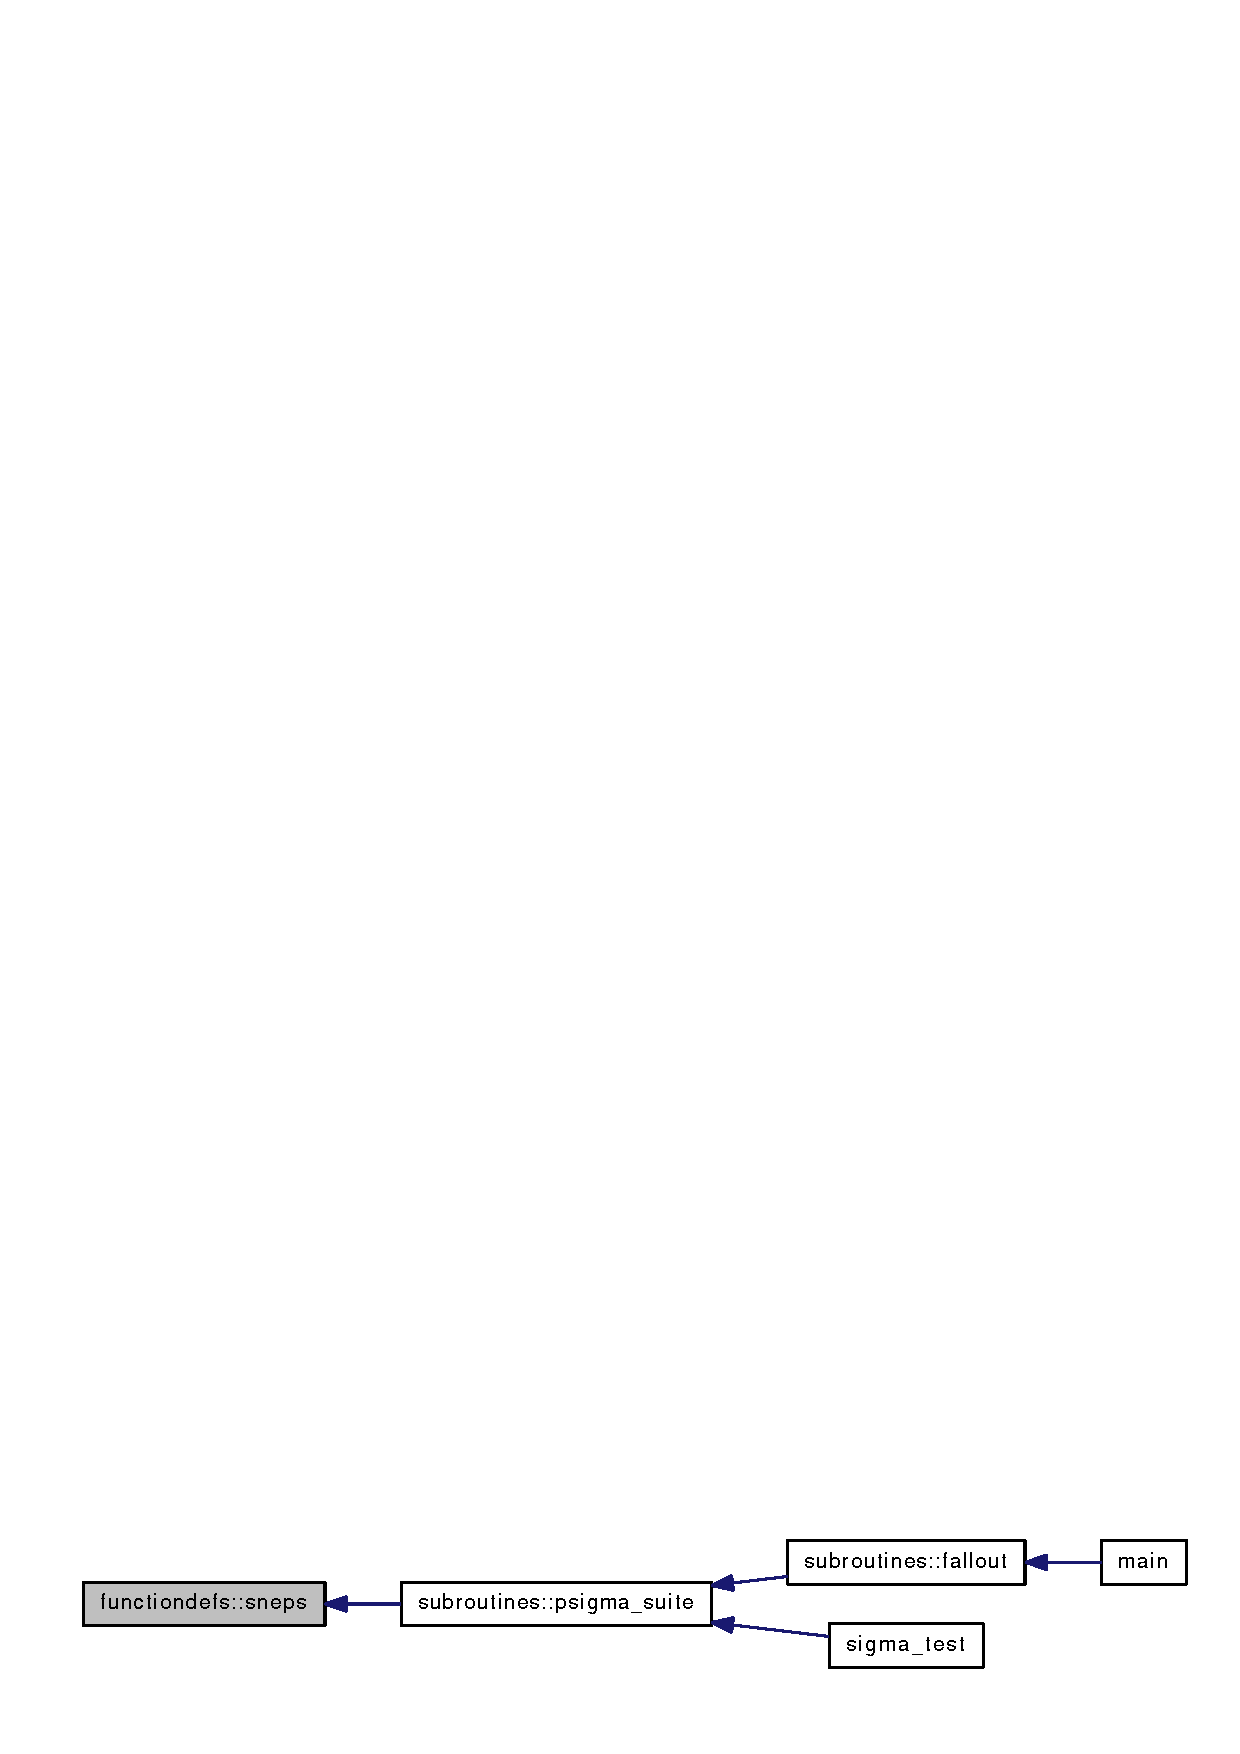
\includegraphics[width=287pt]{namespacefunctiondefs_a80d99fe52a1cb5856694596955d8aeb9_icgraph}
\end{center}
\end{figure}
\hypertarget{namespacefunctiondefs_a5e1c4c25a7352f149e1f18854c37930f}{
\index{functiondefs@{functiondefs}!t\_\-0\_\-gs@{t\_\-0\_\-gs}}
\index{t\_\-0\_\-gs@{t\_\-0\_\-gs}!functiondefs@{functiondefs}}
\subsubsection[{t\_\-0\_\-gs}]{\setlength{\rightskip}{0pt plus 5cm}DOUBLE PRECISION functiondefs::t\_\-0\_\-gs (DOUBLE PRECISION,intent(in) {\em energy}, \/  DOUBLE PRECISION,intent(in) {\em t\_\-a}, \/  DOUBLE PRECISION,intent(in) {\em t\_\-b}, \/  DOUBLE PRECISION,intent(in) {\em t\_\-s})}}
\label{namespacefunctiondefs_a5e1c4c25a7352f149e1f18854c37930f}


Definition at line 120 of file functiondefs.f90.

Referenced by subroutines::esigma\_\-suite().

Here is the caller graph for this function:\nopagebreak
\begin{figure}[H]
\begin{center}
\leavevmode
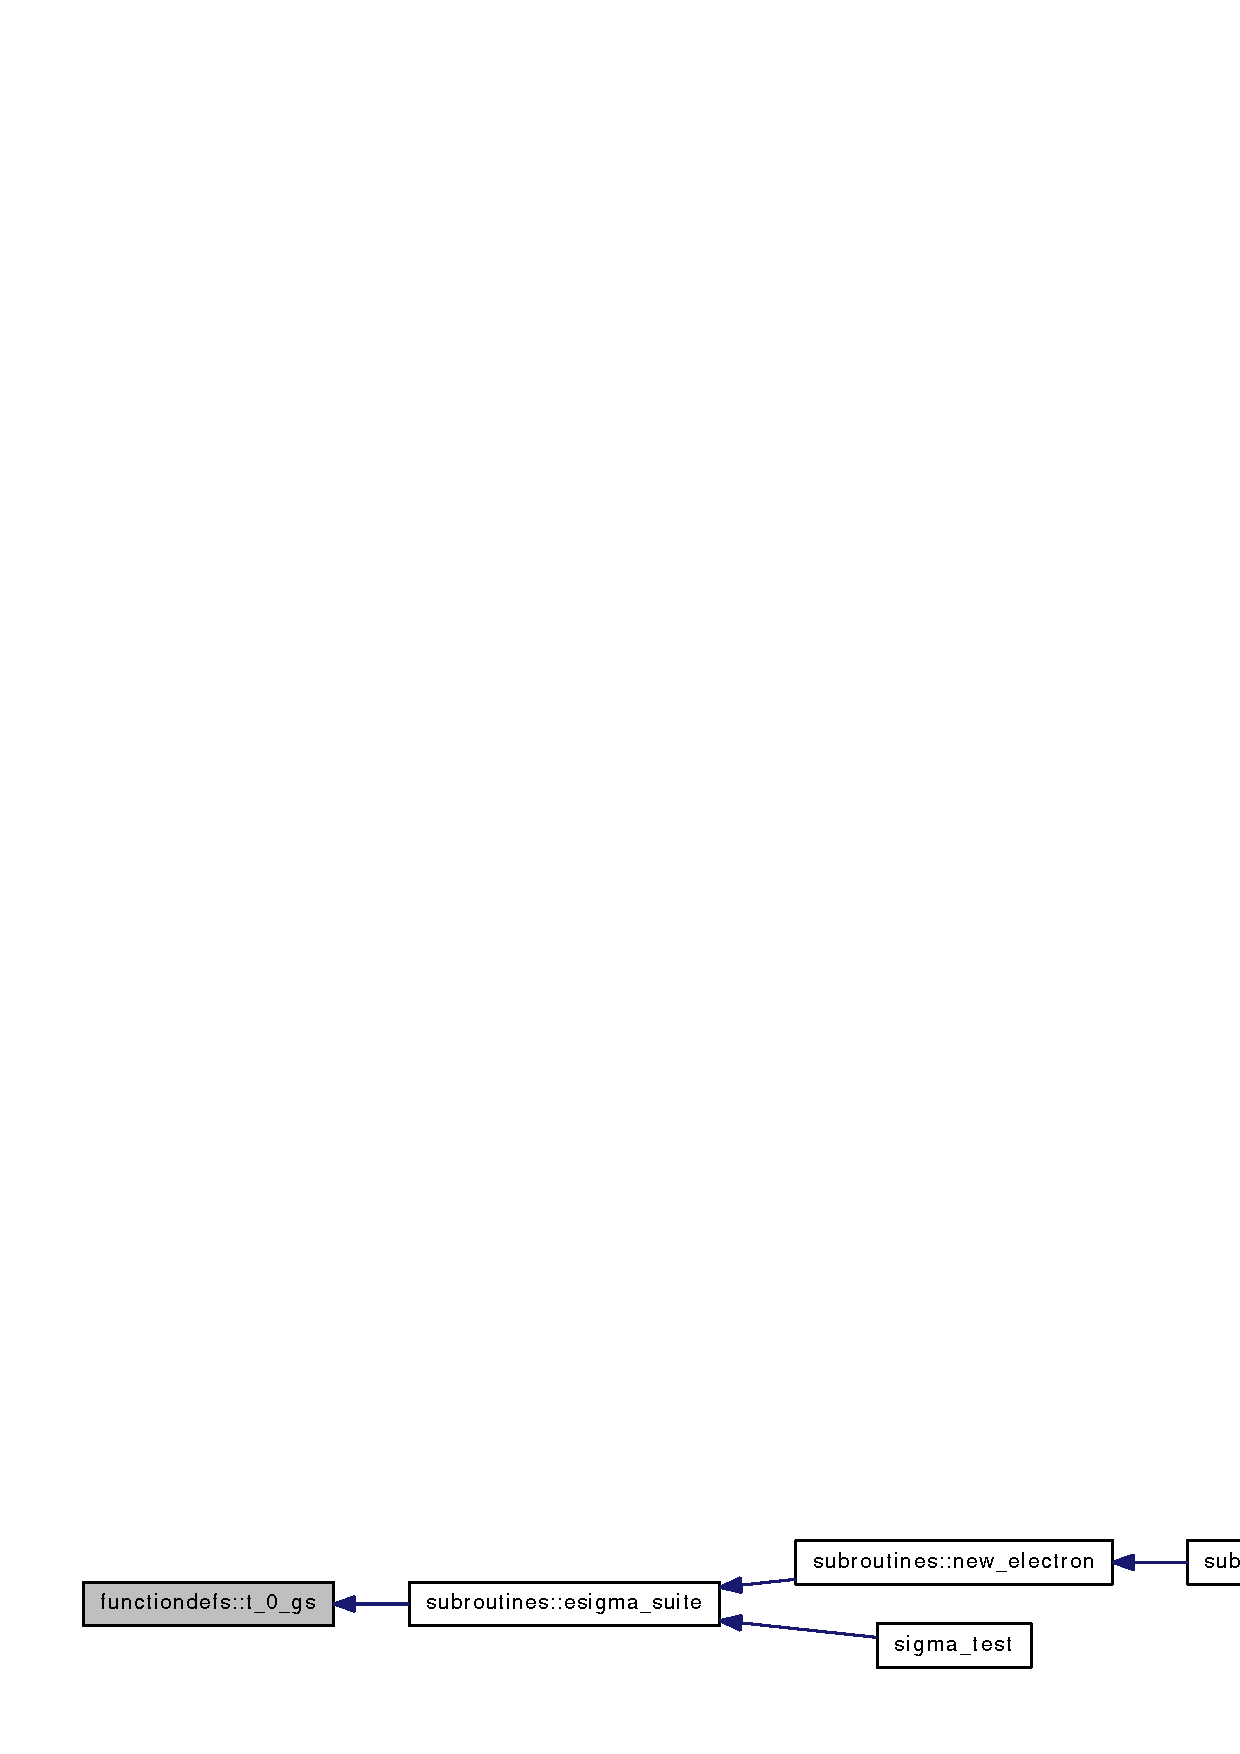
\includegraphics[width=383pt]{namespacefunctiondefs_a5e1c4c25a7352f149e1f18854c37930f_icgraph}
\end{center}
\end{figure}
\hypertarget{namespacefunctiondefs_a529a6bcbb0305c32f0275aa85d4303e8}{
\index{functiondefs@{functiondefs}!t\_\-coll@{t\_\-coll}}
\index{t\_\-coll@{t\_\-coll}!functiondefs@{functiondefs}}
\subsubsection[{t\_\-coll}]{\setlength{\rightskip}{0pt plus 5cm}DOUBLE PRECISION functiondefs::t\_\-coll (DOUBLE PRECISION,pointer {\em e}, \/  DOUBLE PRECISION,intent(in) {\em mf}, \/  DOUBLE PRECISION,intent(in) {\em s2})}}
\label{namespacefunctiondefs_a529a6bcbb0305c32f0275aa85d4303e8}


Definition at line 431 of file functiondefs.f90.

Referenced by subroutines::elastic\_\-event().

Here is the caller graph for this function:\nopagebreak
\begin{figure}[H]
\begin{center}
\leavevmode
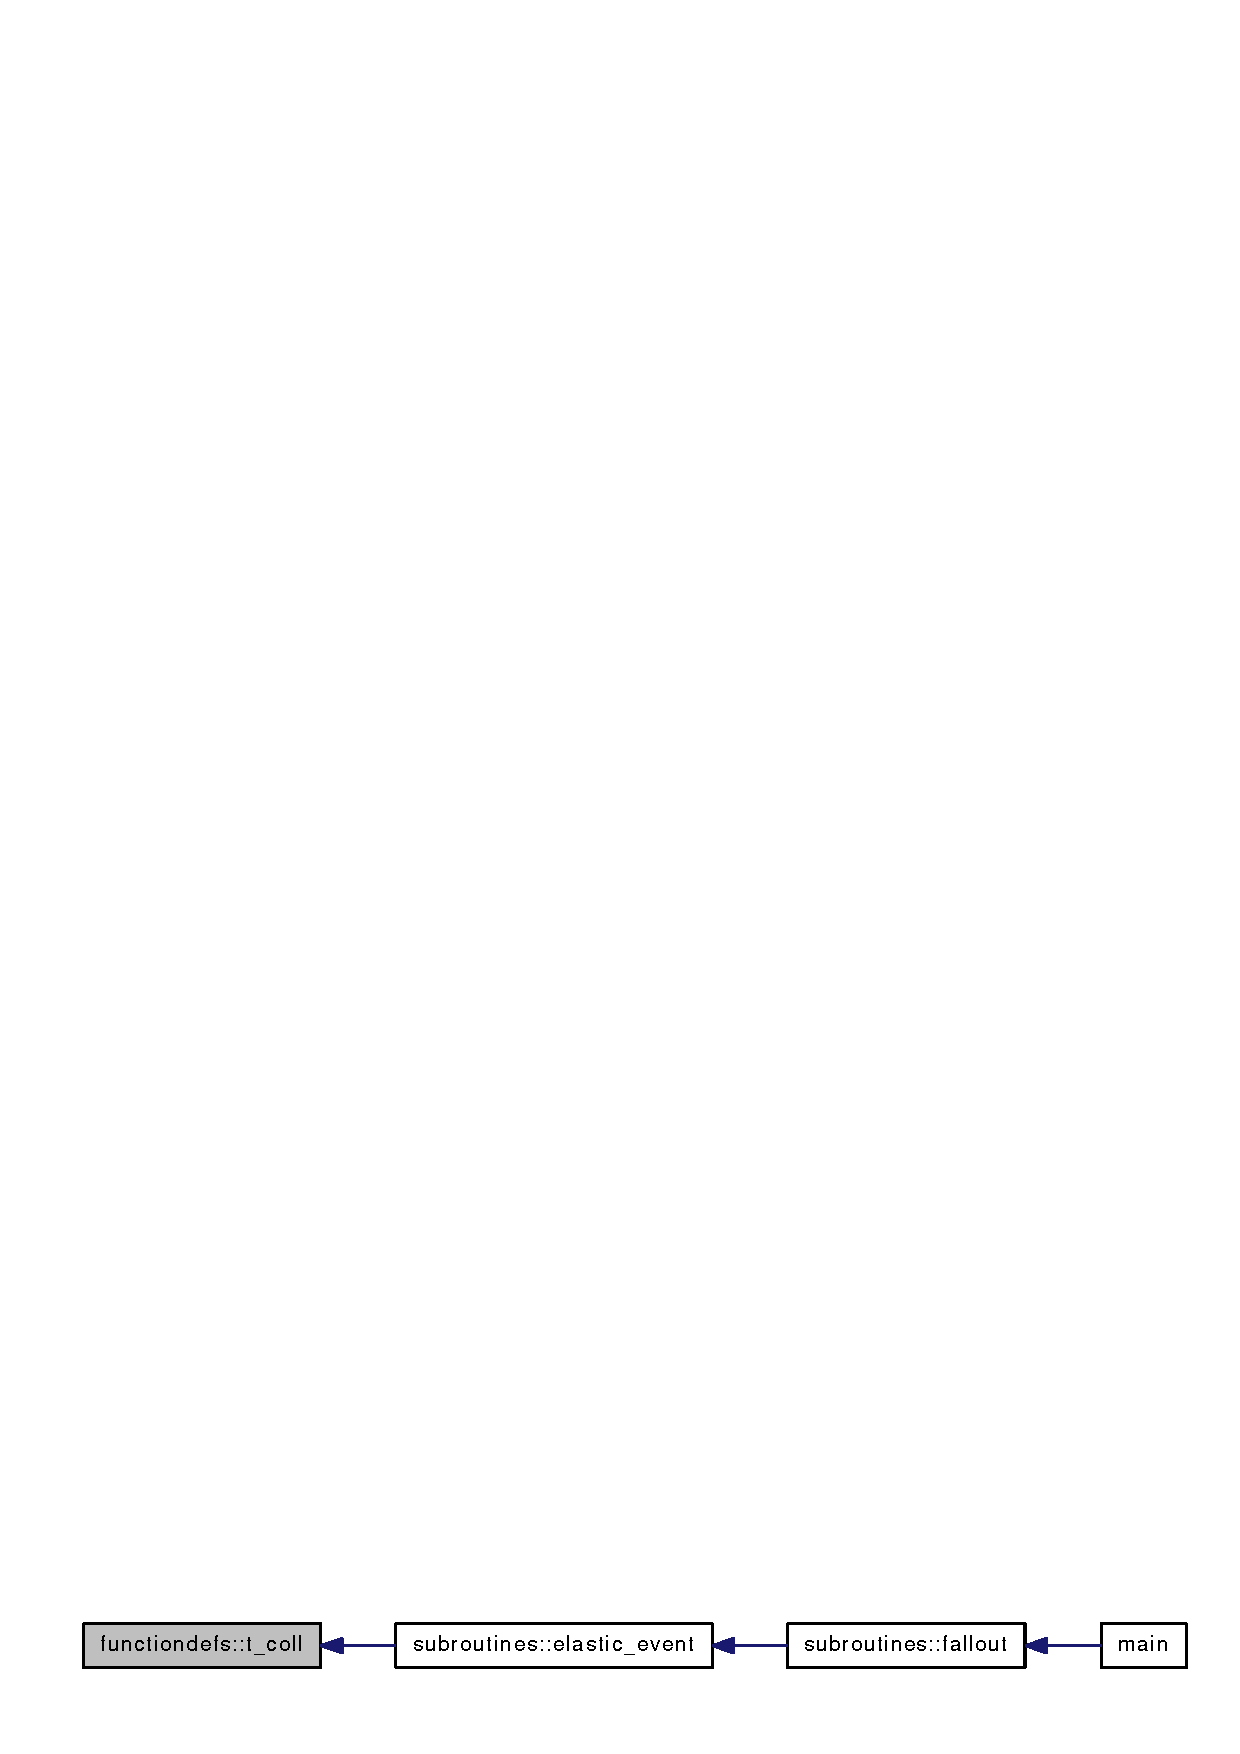
\includegraphics[width=287pt]{namespacefunctiondefs_a529a6bcbb0305c32f0275aa85d4303e8_icgraph}
\end{center}
\end{figure}
\hypertarget{namespacefunctiondefs_a7beb6f6af6e15afda97da88dde407655}{
\index{functiondefs@{functiondefs}!t\_\-max\_\-gs@{t\_\-max\_\-gs}}
\index{t\_\-max\_\-gs@{t\_\-max\_\-gs}!functiondefs@{functiondefs}}
\subsubsection[{t\_\-max\_\-gs}]{\setlength{\rightskip}{0pt plus 5cm}DOUBLE PRECISION functiondefs::t\_\-max\_\-gs (DOUBLE PRECISION,intent(in) {\em energy}, \/  DOUBLE PRECISION,intent(in) {\em i})}}
\label{namespacefunctiondefs_a7beb6f6af6e15afda97da88dde407655}


Definition at line 149 of file functiondefs.f90.

Referenced by subroutines::esigma\_\-suite().

Here is the caller graph for this function:\nopagebreak
\begin{figure}[H]
\begin{center}
\leavevmode
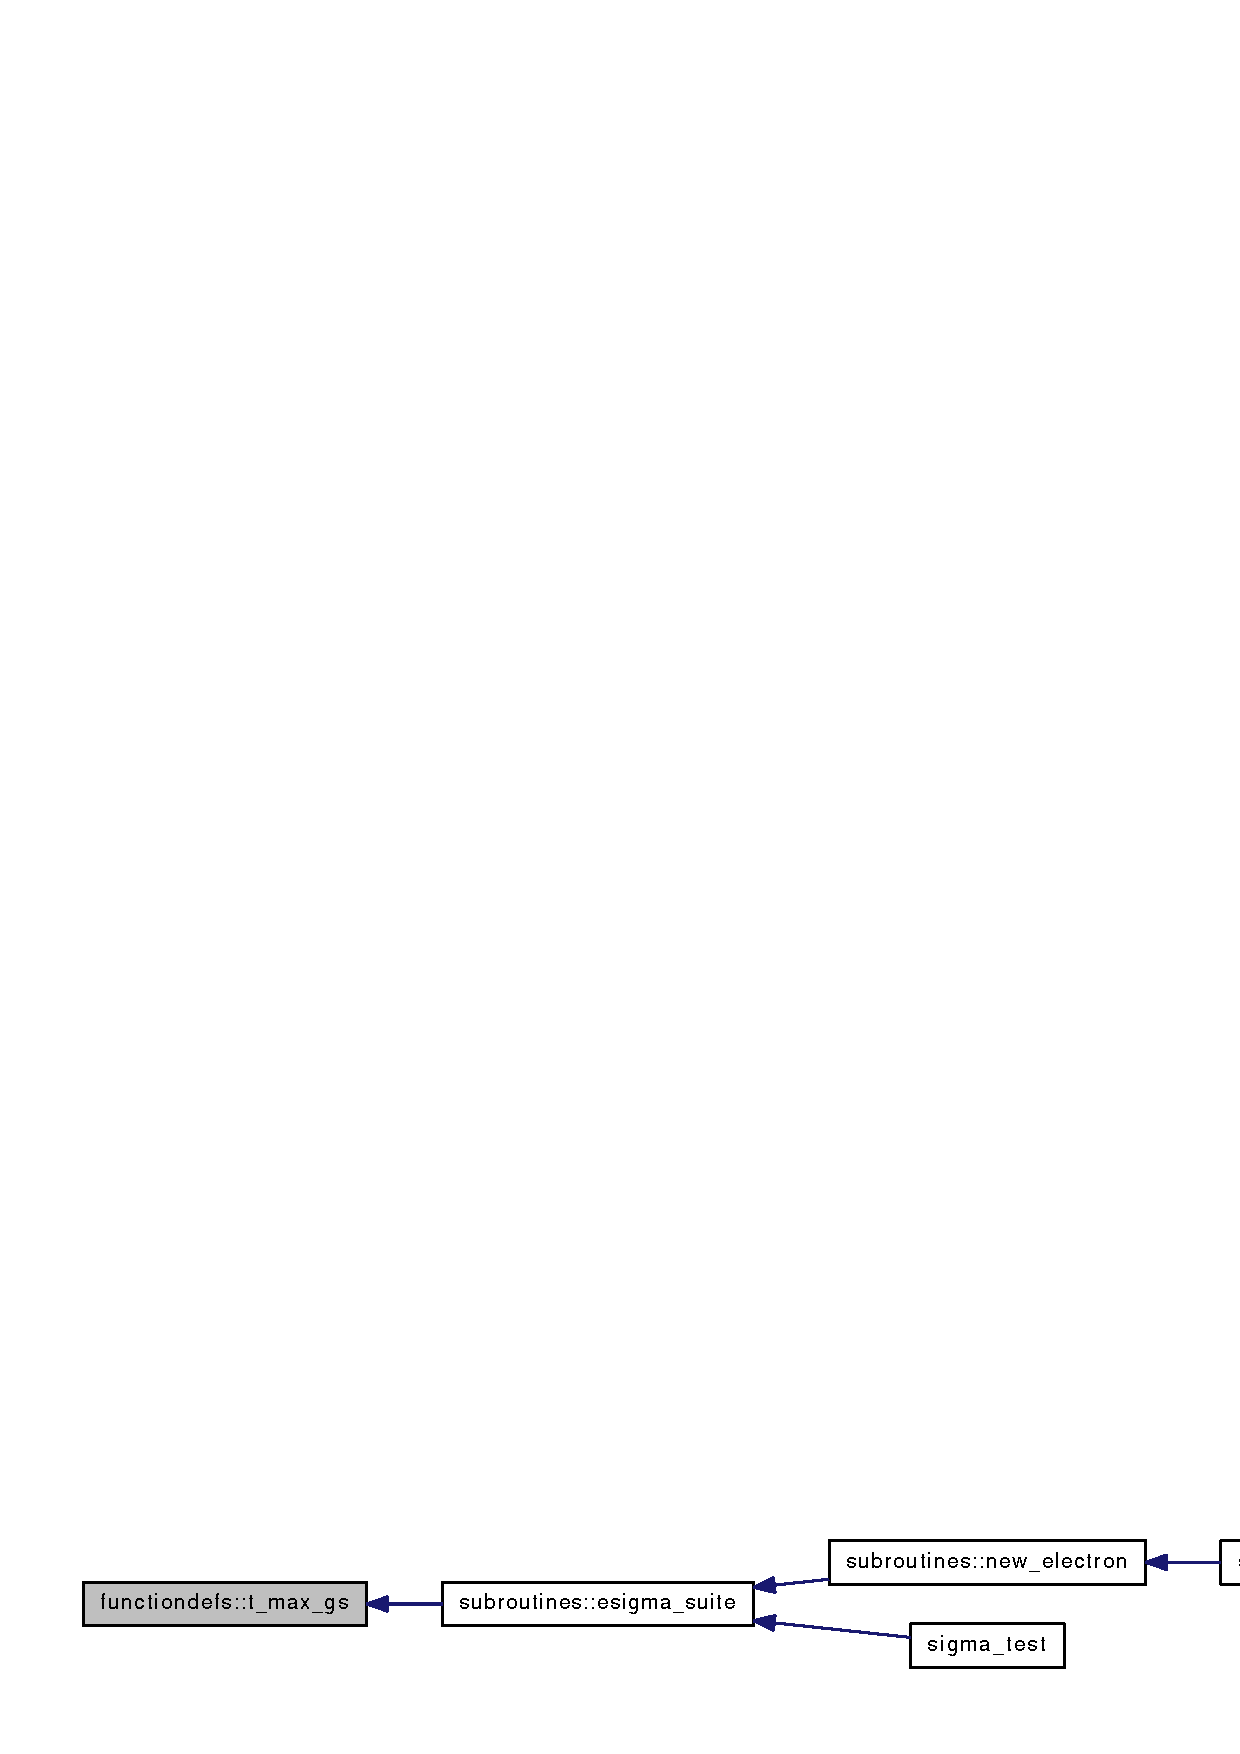
\includegraphics[width=391pt]{namespacefunctiondefs_a7beb6f6af6e15afda97da88dde407655_icgraph}
\end{center}
\end{figure}

\hypertarget{namespacegp}{
\section{gp Module Reference}
\label{namespacegp}\index{gp@{gp}}
}
\subsection*{Functions/Subroutines}
\begin{DoxyCompactItemize}
\item 
subroutine \hyperlink{namespacegp_a0b4ea7e3d8474c9cb6eabeb9581a28b2}{fitness} (unfit, total\_\-fitness)
\item 
subroutine \hyperlink{namespacegp_acef1117d5406847ad3fab8456f70bad7}{store\_\-rand} ()
\end{DoxyCompactItemize}


\subsection{Function/Subroutine Documentation}
\hypertarget{namespacegp_a0b4ea7e3d8474c9cb6eabeb9581a28b2}{
\index{gp@{gp}!fitness@{fitness}}
\index{fitness@{fitness}!gp@{gp}}
\subsubsection[{fitness}]{\setlength{\rightskip}{0pt plus 5cm}subroutine gp::fitness (LOGICAL {\em unfit}, \/  DOUBLE PRECISION,intent(out) {\em total\_\-fitness})}}
\label{namespacegp_a0b4ea7e3d8474c9cb6eabeb9581a28b2}


Definition at line 6 of file gp.f90.

References subroutines::counter(), parameters::EDGE, parameters::FITNESS\_\-THRESHOLD, parameters::FLUENCE, parameters::FLUENCE\_\-TOTAL, parameters::THICK, and parameters::TIME\_\-FREQ.

Referenced by main().

Here is the call graph for this function:\nopagebreak
\begin{figure}[H]
\begin{center}
\leavevmode
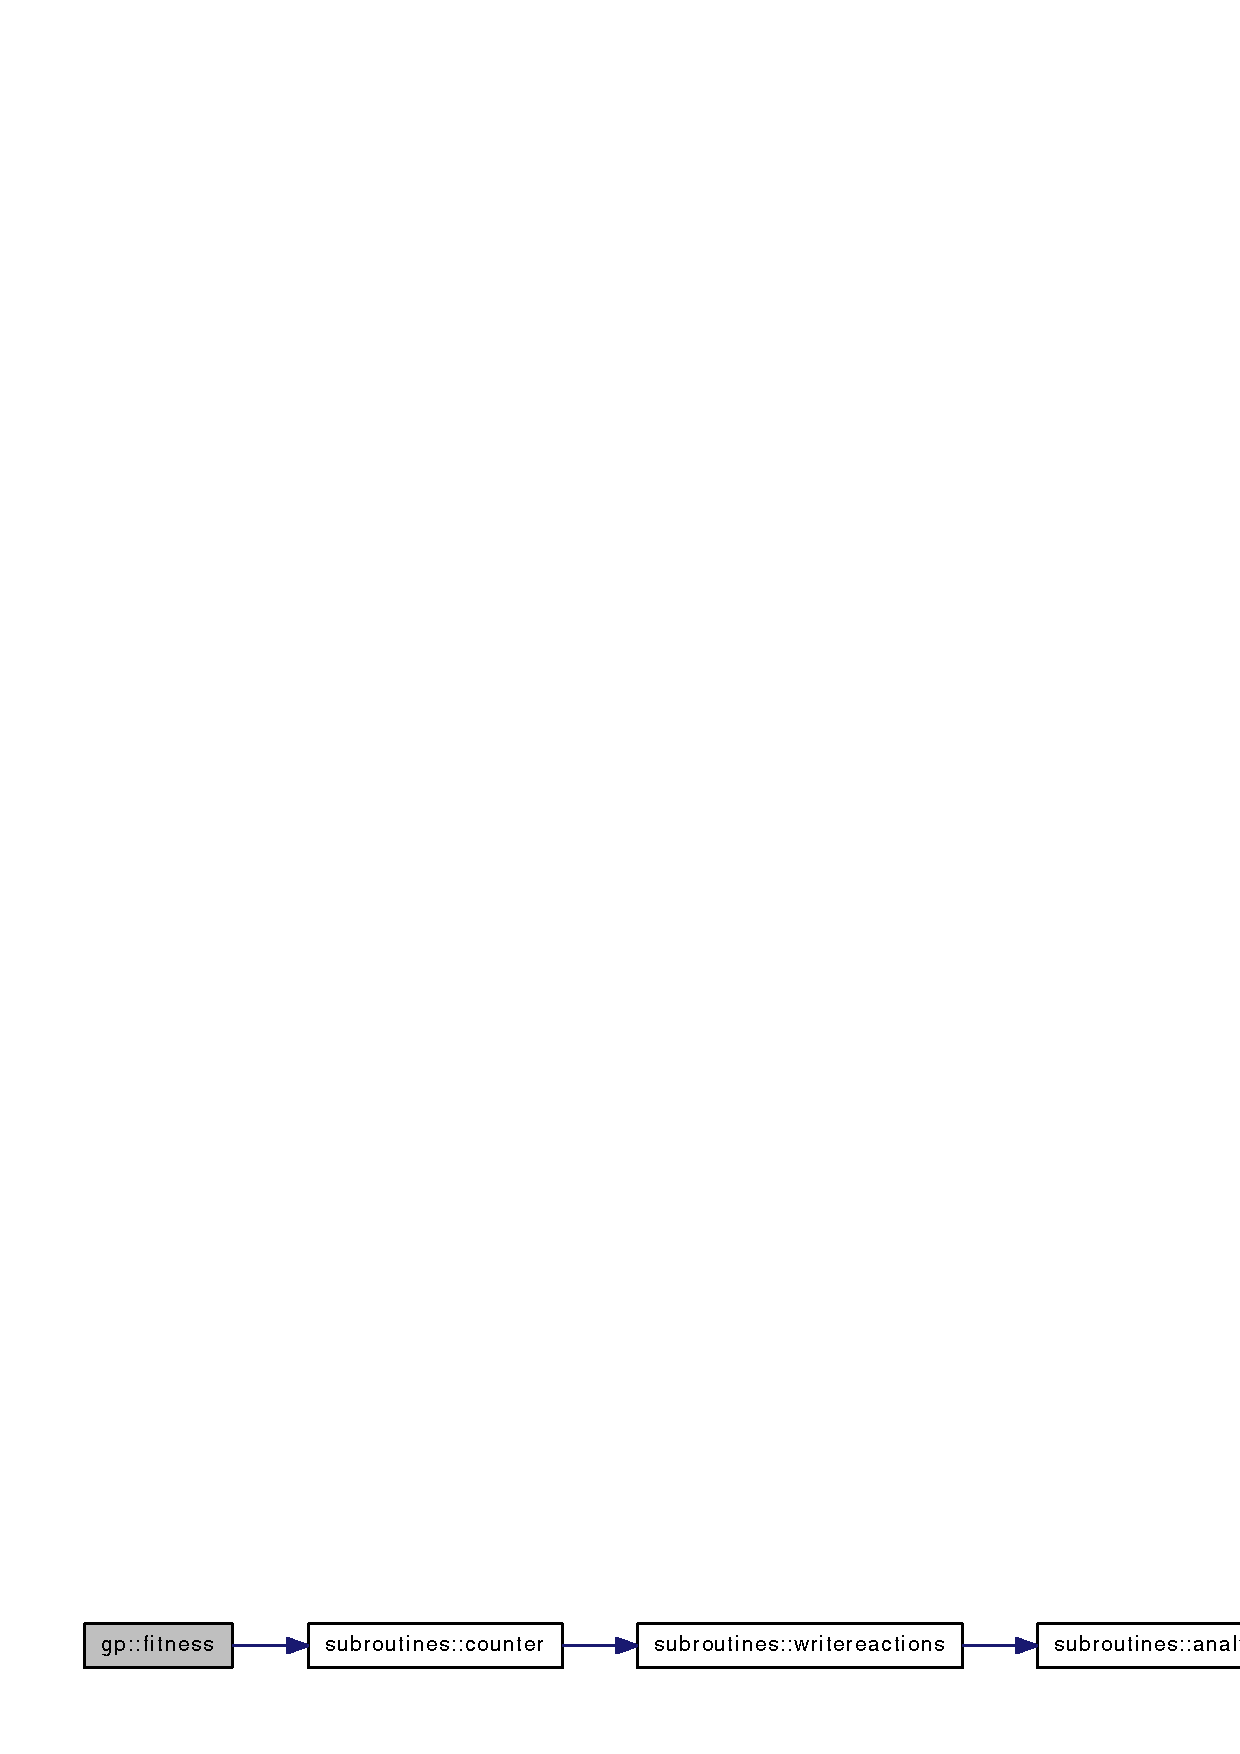
\includegraphics[width=333pt]{namespacegp_a0b4ea7e3d8474c9cb6eabeb9581a28b2_cgraph}
\end{center}
\end{figure}


Here is the caller graph for this function:\nopagebreak
\begin{figure}[H]
\begin{center}
\leavevmode
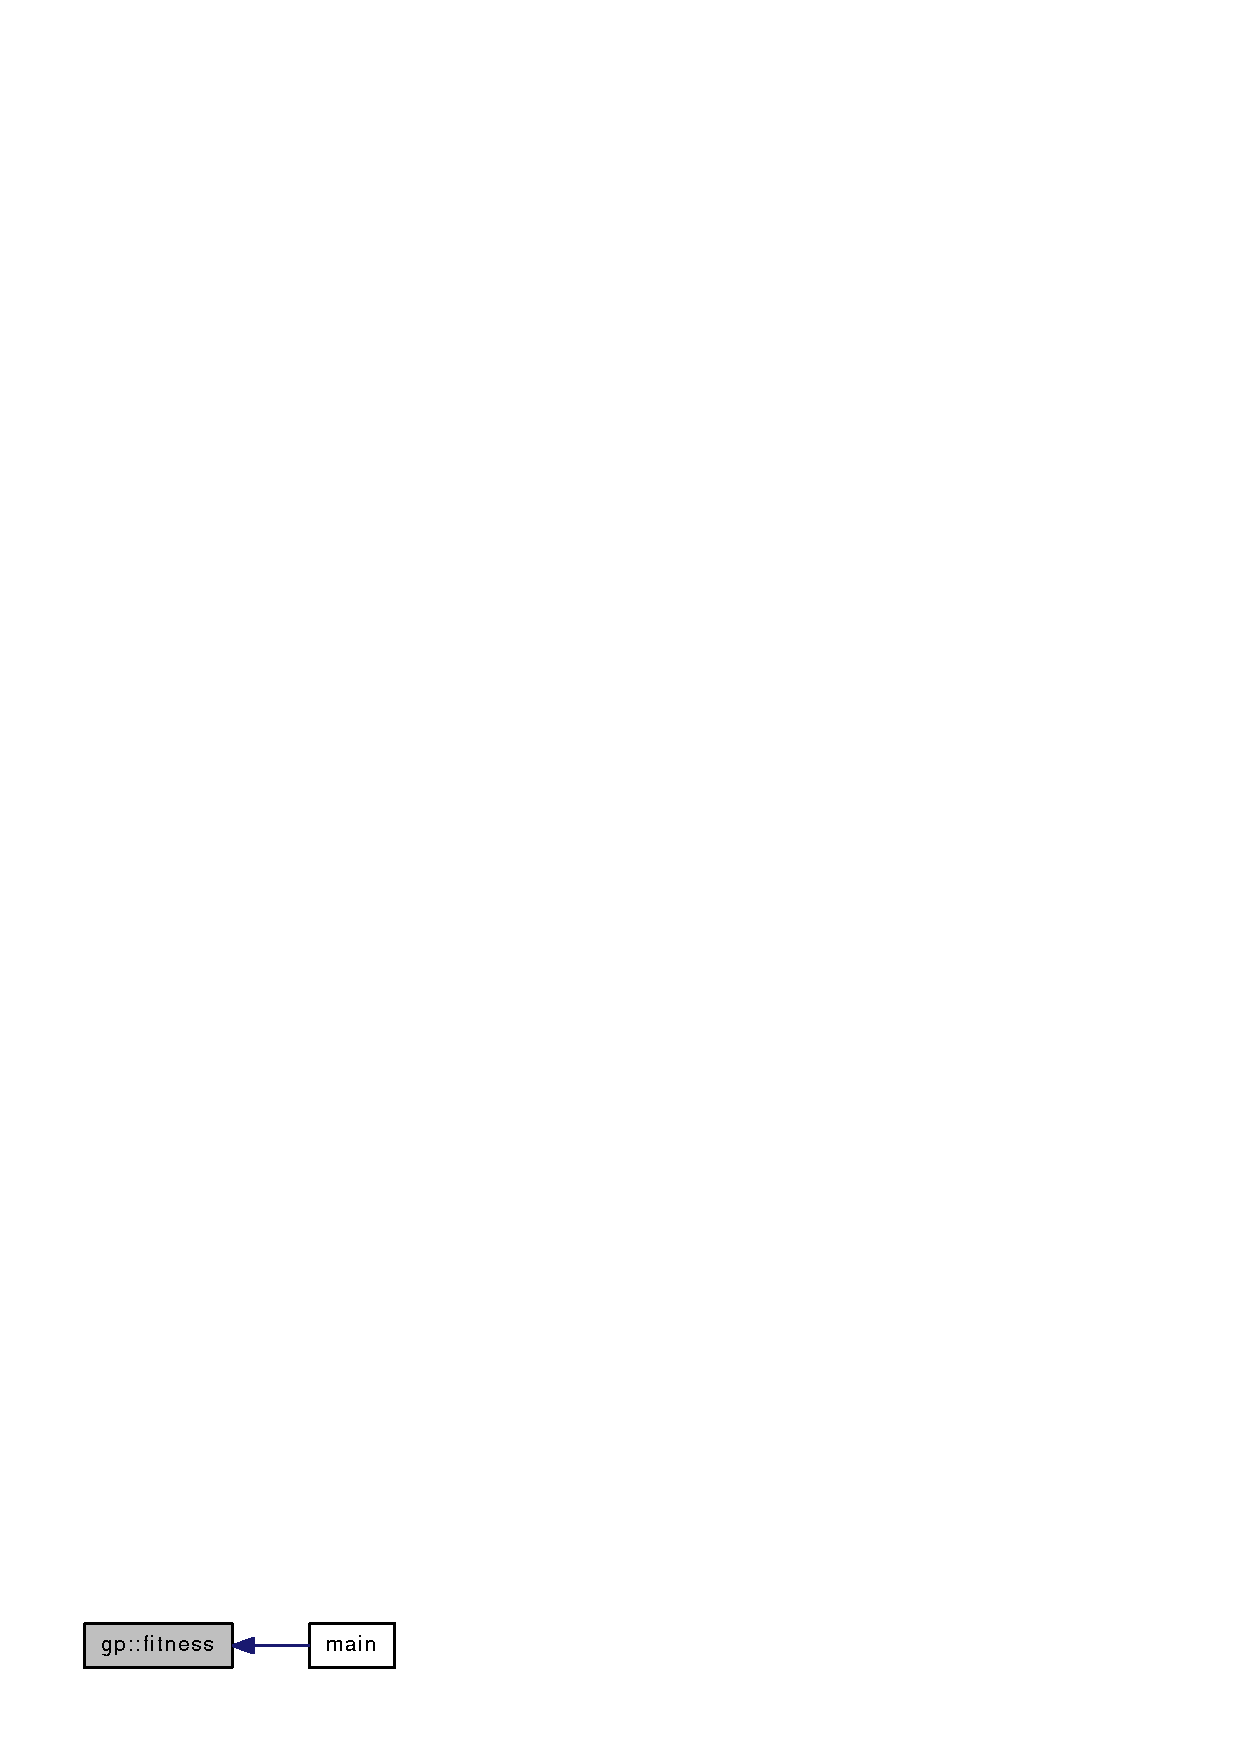
\includegraphics[width=97pt]{namespacegp_a0b4ea7e3d8474c9cb6eabeb9581a28b2_icgraph}
\end{center}
\end{figure}
\hypertarget{namespacegp_acef1117d5406847ad3fab8456f70bad7}{
\index{gp@{gp}!store\_\-rand@{store\_\-rand}}
\index{store\_\-rand@{store\_\-rand}!gp@{gp}}
\subsubsection[{store\_\-rand}]{\setlength{\rightskip}{0pt plus 5cm}subroutine gp::store\_\-rand ()}}
\label{namespacegp_acef1117d5406847ad3fab8456f70bad7}


Definition at line 70 of file gp.f90.
\hypertarget{namespacemc__toolbox}{
\section{mc\_\-toolbox Module Reference}
\label{namespacemc__toolbox}\index{mc\_\-toolbox@{mc\_\-toolbox}}
}
\subsection*{Functions/Subroutines}
\begin{DoxyCompactItemize}
\item 
REAL(KIND=8) \hyperlink{namespacemc__toolbox_acedafdf57f1c1cd3610359fe837a708d}{rgamma} (a)
\item 
real(kind=8) \hyperlink{namespacemc__toolbox_ab8fa538b6e1b30d65864f793e75425ea}{r8\_\-normal\_\-01} ()
\item 
real(kind=8) \hyperlink{namespacemc__toolbox_a405cb2a6c8bceb2f89fc0da987cd399a}{r8\_\-uniform\_\-01} (seedy)
\item 
real(kind=8) \hyperlink{namespacemc__toolbox_aab33e2e1a35352d1550e81fb86fb1cc9}{r8\_\-normal\_\-ab} (a, b)
\end{DoxyCompactItemize}
\subsection*{Variables}
\begin{DoxyCompactItemize}
\item 
INTEGER(KIND=4), parameter \hyperlink{namespacemc__toolbox_a2b3c4edff260f415453579697b0a5282}{GSEED} = 12345
\item 
REAL(KIND=8), parameter \hyperlink{namespacemc__toolbox_a9e72a666484c36244e37a8083e792dd8}{MEANVAL} = 0.00
\item 
REAL(KIND=8), parameter \hyperlink{namespacemc__toolbox_a5655149a57d9d21f98b7515536fe1a1b}{SDEV} = 2.00
\end{DoxyCompactItemize}


\subsection{Function/Subroutine Documentation}
\hypertarget{namespacemc__toolbox_ab8fa538b6e1b30d65864f793e75425ea}{
\index{mc\_\-toolbox@{mc\_\-toolbox}!r8\_\-normal\_\-01@{r8\_\-normal\_\-01}}
\index{r8\_\-normal\_\-01@{r8\_\-normal\_\-01}!mc_toolbox@{mc\_\-toolbox}}
\subsubsection[{r8\_\-normal\_\-01}]{\setlength{\rightskip}{0pt plus 5cm}real ( kind = 8 ) mc\_\-toolbox::r8\_\-normal\_\-01 ()}}
\label{namespacemc__toolbox_ab8fa538b6e1b30d65864f793e75425ea}


Definition at line 48 of file mc\_\-toolbox.f90.\hypertarget{namespacemc__toolbox_aab33e2e1a35352d1550e81fb86fb1cc9}{
\index{mc\_\-toolbox@{mc\_\-toolbox}!r8\_\-normal\_\-ab@{r8\_\-normal\_\-ab}}
\index{r8\_\-normal\_\-ab@{r8\_\-normal\_\-ab}!mc_toolbox@{mc\_\-toolbox}}
\subsubsection[{r8\_\-normal\_\-ab}]{\setlength{\rightskip}{0pt plus 5cm}real ( kind = 8 ) mc\_\-toolbox::r8\_\-normal\_\-ab (real ( kind = 8 ) {\em a}, \/  real ( kind = 8 ) {\em b})}}
\label{namespacemc__toolbox_aab33e2e1a35352d1550e81fb86fb1cc9}


Definition at line 200 of file mc\_\-toolbox.f90.\hypertarget{namespacemc__toolbox_a405cb2a6c8bceb2f89fc0da987cd399a}{
\index{mc\_\-toolbox@{mc\_\-toolbox}!r8\_\-uniform\_\-01@{r8\_\-uniform\_\-01}}
\index{r8\_\-uniform\_\-01@{r8\_\-uniform\_\-01}!mc_toolbox@{mc\_\-toolbox}}
\subsubsection[{r8\_\-uniform\_\-01}]{\setlength{\rightskip}{0pt plus 5cm}real ( kind = 8 ) mc\_\-toolbox::r8\_\-uniform\_\-01 (integer ( kind = 4 ) {\em seedy})}}
\label{namespacemc__toolbox_a405cb2a6c8bceb2f89fc0da987cd399a}


Definition at line 99 of file mc\_\-toolbox.f90.\hypertarget{namespacemc__toolbox_acedafdf57f1c1cd3610359fe837a708d}{
\index{mc\_\-toolbox@{mc\_\-toolbox}!rgamma@{rgamma}}
\index{rgamma@{rgamma}!mc_toolbox@{mc\_\-toolbox}}
\subsubsection[{rgamma}]{\setlength{\rightskip}{0pt plus 5cm}REAL(KIND=8) mc\_\-toolbox::rgamma (REAL(KIND=8),intent(in) {\em a})}}
\label{namespacemc__toolbox_acedafdf57f1c1cd3610359fe837a708d}


Definition at line 9 of file mc\_\-toolbox.f90.

References MEANVAL, and SDEV.

Referenced by subroutines::p\_\-ion\_\-select().

Here is the caller graph for this function:\nopagebreak
\begin{figure}[H]
\begin{center}
\leavevmode
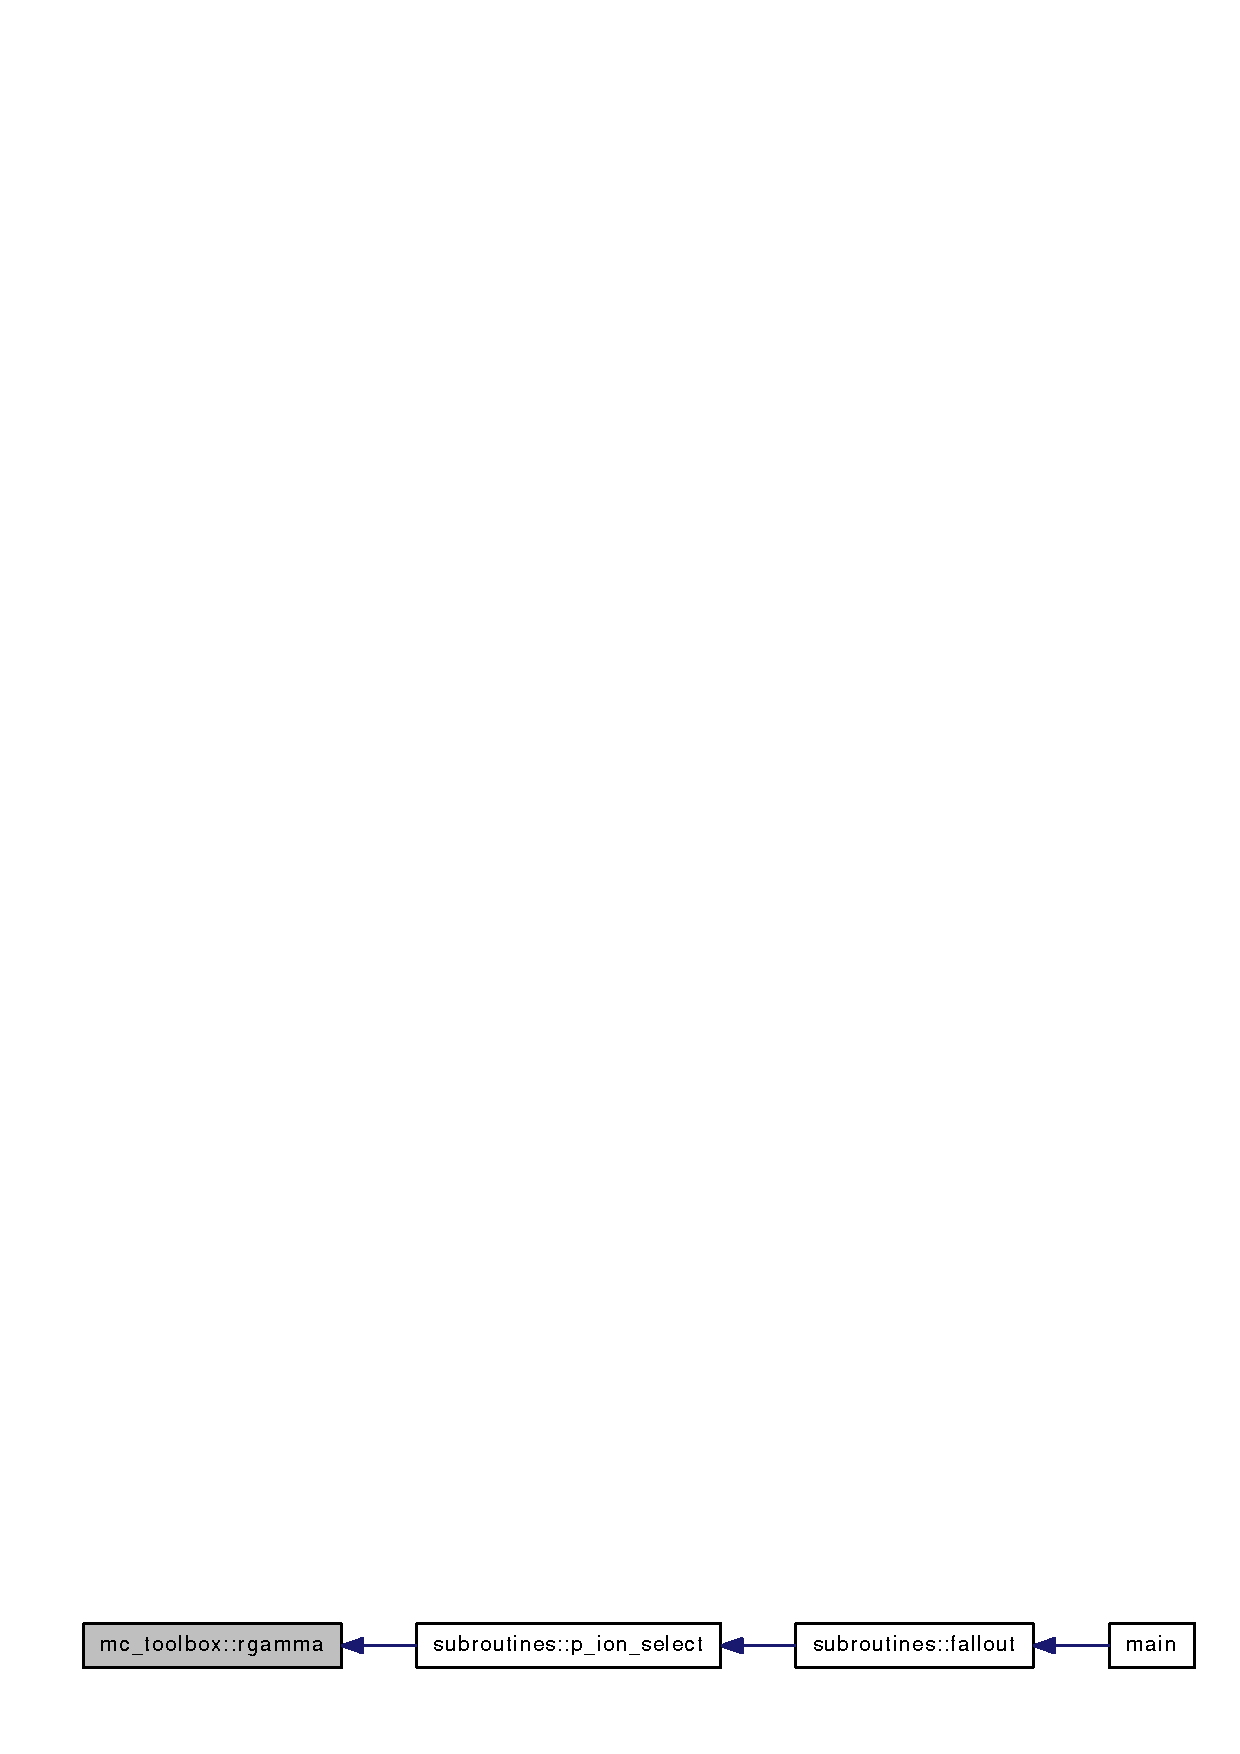
\includegraphics[width=289pt]{namespacemc__toolbox_acedafdf57f1c1cd3610359fe837a708d_icgraph}
\end{center}
\end{figure}


\subsection{Variable Documentation}
\hypertarget{namespacemc__toolbox_a2b3c4edff260f415453579697b0a5282}{
\index{mc\_\-toolbox@{mc\_\-toolbox}!GSEED@{GSEED}}
\index{GSEED@{GSEED}!mc_toolbox@{mc\_\-toolbox}}
\subsubsection[{GSEED}]{\setlength{\rightskip}{0pt plus 5cm}INTEGER(KIND=4),parameter {\bf mc\_\-toolbox::GSEED} = 12345}}
\label{namespacemc__toolbox_a2b3c4edff260f415453579697b0a5282}


Definition at line 4 of file mc\_\-toolbox.f90.\hypertarget{namespacemc__toolbox_a9e72a666484c36244e37a8083e792dd8}{
\index{mc\_\-toolbox@{mc\_\-toolbox}!MEANVAL@{MEANVAL}}
\index{MEANVAL@{MEANVAL}!mc_toolbox@{mc\_\-toolbox}}
\subsubsection[{MEANVAL}]{\setlength{\rightskip}{0pt plus 5cm}REAL(KIND=8),parameter {\bf mc\_\-toolbox::MEANVAL} = 0.00}}
\label{namespacemc__toolbox_a9e72a666484c36244e37a8083e792dd8}


Definition at line 5 of file mc\_\-toolbox.f90.

Referenced by rgamma().\hypertarget{namespacemc__toolbox_a5655149a57d9d21f98b7515536fe1a1b}{
\index{mc\_\-toolbox@{mc\_\-toolbox}!SDEV@{SDEV}}
\index{SDEV@{SDEV}!mc_toolbox@{mc\_\-toolbox}}
\subsubsection[{SDEV}]{\setlength{\rightskip}{0pt plus 5cm}REAL(KIND=8),parameter {\bf mc\_\-toolbox::SDEV} = 2.00}}
\label{namespacemc__toolbox_a5655149a57d9d21f98b7515536fe1a1b}


Definition at line 6 of file mc\_\-toolbox.f90.

Referenced by rgamma().
\hypertarget{namespacenewmod}{
\section{newmod Module Reference}
\label{namespacenewmod}\index{newmod@{newmod}}
}
\subsection*{Data Types}
\begin{DoxyCompactItemize}
\item 
type \hyperlink{typenewmod_1_1species}{species}
\item 
type \hyperlink{typenewmod_1_1reaction}{reaction}
\end{DoxyCompactItemize}
\subsection*{Functions/Subroutines}
\begin{DoxyCompactItemize}
\item 
subroutine \hyperlink{namespacenewmod_a6e08d1c91ffcb8d044e3ad8d8b535348}{lookup} (name, node, id)
\end{DoxyCompactItemize}


\subsection{Function/Subroutine Documentation}
\hypertarget{namespacenewmod_a6e08d1c91ffcb8d044e3ad8d8b535348}{
\index{newmod@{newmod}!lookup@{lookup}}
\index{lookup@{lookup}!newmod@{newmod}}
\subsubsection[{lookup}]{\setlength{\rightskip}{0pt plus 5cm}subroutine newmod::lookup (CHARACTER(len=10) {\em name}, \/  TYPE(species) {\em node}, \/  INTEGER {\em id})}}
\label{namespacenewmod_a6e08d1c91ffcb8d044e3ad8d8b535348}


Definition at line 32 of file newmod.f90.

Referenced by newnet().

Here is the caller graph for this function:\nopagebreak
\begin{figure}[H]
\begin{center}
\leavevmode
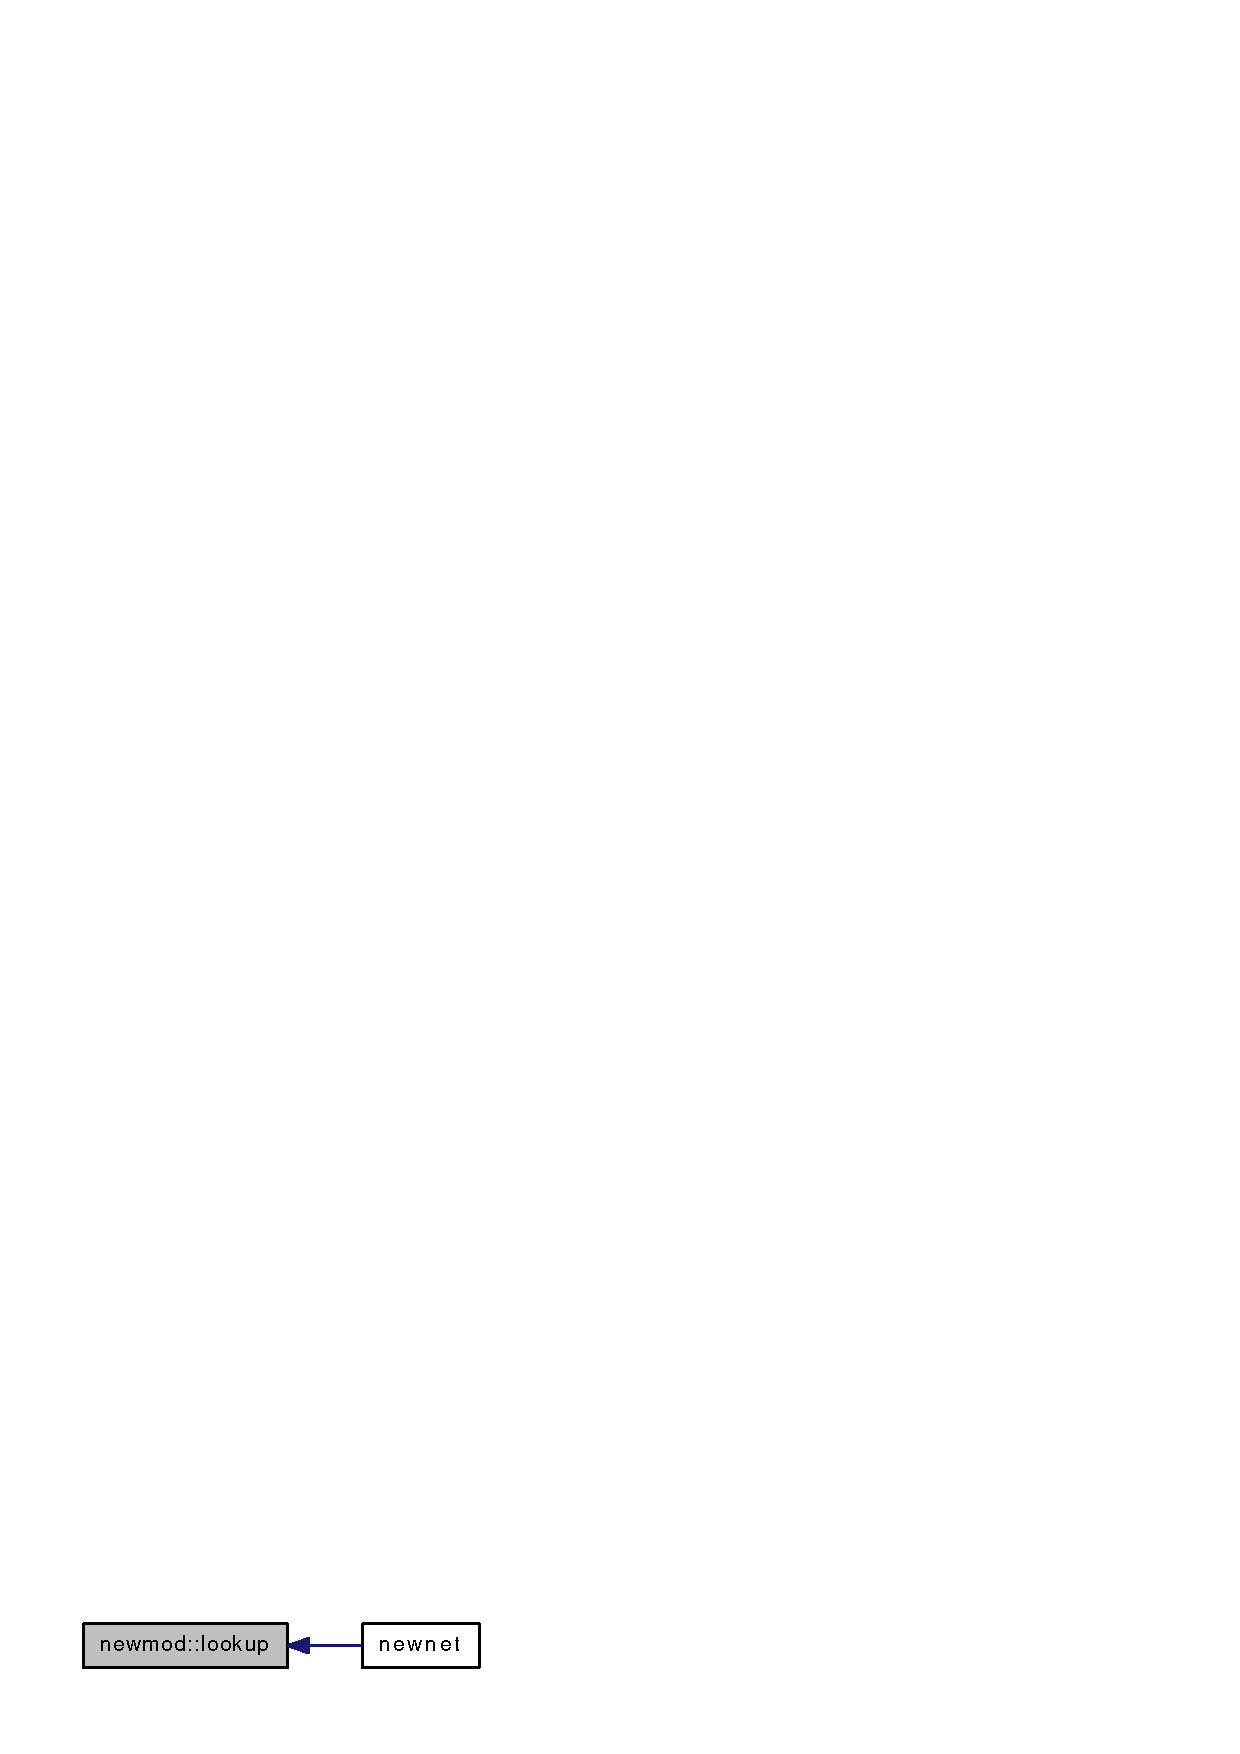
\includegraphics[width=117pt]{namespacenewmod_a6e08d1c91ffcb8d044e3ad8d8b535348_icgraph}
\end{center}
\end{figure}

\hypertarget{namespaceparameters}{
\section{parameters Module Reference}
\label{namespaceparameters}\index{parameters@{parameters}}
}
\subsection*{Variables}
\begin{DoxyCompactItemize}
\item 
TYPE(\hyperlink{typetypedefs_1_1node}{node}), allocatable, target \hyperlink{namespaceparameters_a1d2ec6532bce135a8fc18f3542969a8d}{MATRIX}
\item 
INTEGER \hyperlink{namespaceparameters_a8eba14af35a7a362f50093f1acc28a78}{DIMENS}
\item 
INTEGER \hyperlink{namespaceparameters_a00c44079184906f8aff60ad7cea2fe4d}{PRODS}
\item 
DOUBLE PRECISION, allocatable \hyperlink{namespaceparameters_a41b06e1dd582bb56419bf991f2c633e3}{EN\_\-LIST}
\item 
CHARACTER(LEN=10), allocatable \hyperlink{namespaceparameters_a38878c1dc241cdcfc52f1804563f7b00}{SP\_\-LIST}
\item 
INTEGER, allocatable \hyperlink{namespaceparameters_a660ab08d014ed8f467dc504ed8585591}{IONLIST}
\item 
INTEGER, allocatable \hyperlink{namespaceparameters_a649c343c05b95e3f84d06401b3a3f6e1}{SP\_\-PROD\_\-DEST}
\item 
integer, dimension(:), allocatable \hyperlink{namespaceparameters_a8706bba63c5517e5b5e5b2cf0487db4b}{fast\_\-reacts}
\item 
INTEGER \hyperlink{namespaceparameters_aed3ebeff9daeb47edfa593ae2b72d4db}{NUM\_\-SPECIES} = 0
\item 
INTEGER \hyperlink{namespaceparameters_a1462d3a8d5ef4ee00ffc9c0beac695b2}{NUM\_\-REACTS} = 0
\item 
INTEGER \hyperlink{namespaceparameters_abf21c9c60fbc062ca9e84d2746c7388a}{NUMPROTONS} = 0
\item 
DOUBLE PRECISION \hyperlink{namespaceparameters_acf1d338d691bf2082aeabaec6ac27263}{TIME} = 0
\item 
TYPE(\hyperlink{typetypedefs_1_1reaction}{reaction}), pointer \hyperlink{namespaceparameters_aff68a046aeb1fa2a7610db8cd55922d8}{RE\_\-HEAD}
\item 
integer \hyperlink{namespaceparameters_a2a130bb0e6ad790a2a783d19749cc8ce}{initialatoms} = 0
\item 
REAL \hyperlink{namespaceparameters_a3c39b69e0083dc018e4546bd5a02b301}{GVALUE} = 0
\item 
REAL \hyperlink{namespaceparameters_a2855e0778fdd644c62b1a6943a4c363a}{CUIRCT} = 0
\item 
REAL \hyperlink{namespaceparameters_a170cb61fd1eef5175a5eaf95d0d85ab5}{CUPREL} = 0
\item 
INTEGER \hyperlink{namespaceparameters_a38fbcf3f41331f232ff4c604194bc76f}{PMODEL} = 0
\item 
CHARACTER(LEN=80), parameter \hyperlink{namespaceparameters_af23a39fc248303c9a69e3e05c0fb3b41}{SPECIES\_\-FILE}
\item 
CHARACTER(LEN=80), parameter \hyperlink{namespaceparameters_a40ef599fa2e91d0f27cbd322f1270da8}{REACTIONS\_\-FILE}
\item 
CHARACTER(LEN=80), parameter \hyperlink{namespaceparameters_adf79c33c6ebf2e4f00fa0fdaf34d1ba1}{PARAMS\_\-FILE}
\item 
CHARACTER(LEN=80), parameter \hyperlink{namespaceparameters_a045269697aa491915bf603f55e12b63a}{GEMINACY\_\-FILE}
\item 
DOUBLE PRECISION, parameter \hyperlink{namespaceparameters_a5f4fb781d85daf37e0a18e15e4dcc9c8}{EINIT} = 100D3
\item 
DOUBLE PRECISION, parameter \hyperlink{namespaceparameters_a1f6362692e1384b097b58b185096b416}{CDIM} = 3.414e-\/8
\item 
DOUBLE PRECISION, parameter \hyperlink{namespaceparameters_a3a667857cb5e332f397b7ff0e96dbb85}{BDIM} = 6.668e-\/8
\item 
DOUBLE PRECISION, parameter \hyperlink{namespaceparameters_ad2ed15127be0caca99788b8acc6e605b}{ADIM} = 9.225e-\/8
\item 
DOUBLE PRECISION, parameter \hyperlink{namespaceparameters_aaa3c163a9f90b6d0c5a314ca449da18b}{BETACRYS} = 85.05
\item 
DOUBLE PRECISION, parameter \hyperlink{namespaceparameters_a998d2db873404e0cfe943d50d3877262}{C\_\-PR} = \hyperlink{namespaceparameters_a1f6362692e1384b097b58b185096b416}{CDIM}$\ast$COS(90-\/\hyperlink{namespaceparameters_aaa3c163a9f90b6d0c5a314ca449da18b}{BETACRYS})
\item 
DOUBLE PRECISION, parameter \hyperlink{namespaceparameters_ad8323286536365bb131984aa57af99df}{RHO} = 1.313E22
\item 
DOUBLE PRECISION, parameter \hyperlink{namespaceparameters_a79fa48b917f68e1a12577e33fd8c991c}{RHO2} = 0.01313
\item 
INTEGER, parameter \hyperlink{namespaceparameters_a2fbeb743f79ed8a1c34482eb24ce3e87}{FIX1} = 150
\item 
INTEGER, parameter \hyperlink{namespaceparameters_a11cddb5a155baade8a969acb80c17292}{FIX2} = 150
\item 
INTEGER, parameter \hyperlink{namespaceparameters_adedf5e0e6373ffbf611e8767d9cf0e80}{FIX3} = 150
\item 
DOUBLE PRECISION, parameter \hyperlink{namespaceparameters_aacbd355b27d7e7459076fdf3f77fab20}{THICK} = 1.0e-\/5
\item 
DOUBLE PRECISION, parameter \hyperlink{namespaceparameters_a45377074e21edf9bd71351430490cd5e}{EDGE} = 3.5e-\/6
\item 
DOUBLE PRECISION, parameter \hyperlink{namespaceparameters_a8a887d07bb62f10ae5578c2a7181a578}{VOLUME} = \hyperlink{namespaceparameters_aacbd355b27d7e7459076fdf3f77fab20}{THICK}$\ast$\hyperlink{namespaceparameters_a45377074e21edf9bd71351430490cd5e}{EDGE}$\ast$\hyperlink{namespaceparameters_a45377074e21edf9bd71351430490cd5e}{EDGE}
\item 
DOUBLE PRECISION, parameter \hyperlink{namespaceparameters_a144dd87a3ad4a40138cad0b8d26ee282}{KIN\_\-TEMP} = 5.0D0
\item 
DOUBLE PRECISION, parameter \hyperlink{namespaceparameters_aee8d50a231f8beed7edc0ff5ba2437f4}{AREA} = \hyperlink{namespaceparameters_a45377074e21edf9bd71351430490cd5e}{EDGE}$\ast$\hyperlink{namespaceparameters_a45377074e21edf9bd71351430490cd5e}{EDGE}
\item 
DOUBLE PRECISION, parameter \hyperlink{namespaceparameters_ad9a62be82a2fb56fe291f73d3279d4b4}{CR\_\-FLUX} = 1.0D11
\item 
DOUBLE PRECISION, parameter \hyperlink{namespaceparameters_ac433c7adc61bc138dfc7567a570833ed}{CR\_\-RATE} = \hyperlink{namespaceparameters_ad9a62be82a2fb56fe291f73d3279d4b4}{CR\_\-FLUX}$\ast$\hyperlink{namespaceparameters_aee8d50a231f8beed7edc0ff5ba2437f4}{AREA}
\item 
DOUBLE PRECISION, parameter \hyperlink{namespaceparameters_a20c80b2e34c240feef7ac6887646115d}{NELEM} = 3.0$\ast$\hyperlink{namespaceparameters_ad8323286536365bb131984aa57af99df}{RHO}$\ast$(\hyperlink{namespaceparameters_aacbd355b27d7e7459076fdf3f77fab20}{THICK}$\ast$\hyperlink{namespaceparameters_a45377074e21edf9bd71351430490cd5e}{EDGE}$\ast$\hyperlink{namespaceparameters_a45377074e21edf9bd71351430490cd5e}{EDGE})
\item 
DOUBLE PRECISION, parameter \hyperlink{namespaceparameters_adc91f63a6d2c197941c445a5d64800a3}{TER} = \hyperlink{namespaceparameters_aacbd355b27d7e7459076fdf3f77fab20}{THICK}/\hyperlink{namespaceparameters_a45377074e21edf9bd71351430490cd5e}{EDGE}
\item 
INTEGER, parameter \hyperlink{namespaceparameters_a3f72bf9fb376fde5e0eaf3da242d4f06}{NEDGE} = FLOOR((\hyperlink{namespaceparameters_a20c80b2e34c240feef7ac6887646115d}{NELEM}/\hyperlink{namespaceparameters_adc91f63a6d2c197941c445a5d64800a3}{TER})$\ast$$\ast$(1./3.))
\item 
INTEGER, parameter \hyperlink{namespaceparameters_adf37b75c4792b28d45484737d230ead3}{NTHICK} = FLOOR(\hyperlink{namespaceparameters_a3f72bf9fb376fde5e0eaf3da242d4f06}{NEDGE}$\ast$\hyperlink{namespaceparameters_adc91f63a6d2c197941c445a5d64800a3}{TER})
\item 
REAL, parameter \hyperlink{namespaceparameters_a10dd39ec5aeb14b9a104618dc6ef5450}{E\_\-SURF} = 0.5
\item 
REAL, parameter \hyperlink{namespaceparameters_a485a71bfcc9a08ed577efe9a5df5735b}{E\_\-BULK} = 0.7
\item 
DOUBLE PRECISION, parameter \hyperlink{namespaceparameters_a8b8f35affe261eb9ad1a1612ca3572a7}{SHORT\_\-TIME} = 100.0
\item 
DOUBLE PRECISION, parameter \hyperlink{namespaceparameters_af5f3e31c772340991fe768468c6a0dad}{ZP} = 1.D0
\item 
DOUBLE PRECISION, parameter \hyperlink{namespaceparameters_a1c9d90c36ce0be5595ed197469b6e609}{ZO1} = 8.D0
\item 
DOUBLE PRECISION, parameter \hyperlink{namespaceparameters_a885e127ecd6c6a8469ca5ed6aba4badf}{ZO2} = 16.D0
\item 
DOUBLE PRECISION, parameter \hyperlink{namespaceparameters_ac4b8f44af44db753a988dc78c534c94d}{ZO3} = 24.D0
\item 
DOUBLE PRECISION, parameter \hyperlink{namespaceparameters_a3a8aa693f08c619d7a21b16784fc6cfe}{ENERG} = 100$\ast$1E3
\item 
DOUBLE PRECISION, parameter \hyperlink{namespaceparameters_a55c34135e7a3b750b692c7fe5c44d996}{MP} = 1
\item 
DOUBLE PRECISION, parameter \hyperlink{namespaceparameters_a9fe3ba34735e9bd271a5dfa94242d60f}{MO3} = 24
\item 
DOUBLE PRECISION, parameter \hyperlink{namespaceparameters_a8f3ca9bcf2af3dccca1f89e678dd9149}{MO2} = 16
\item 
DOUBLE PRECISION, parameter \hyperlink{namespaceparameters_a6d254c62ce30ae2227377164deadbabe}{MO1} = 8
\item 
DOUBLE PRECISION, parameter \hyperlink{namespaceparameters_a04ab380d92467d452e23f88704ceb37a}{A0} = 0.529177
\item 
DOUBLE PRECISION, parameter \hyperlink{namespaceparameters_a3012689c3933acd7a66b7268835760a1}{ECHARG2} = 14.39
\item 
DOUBLE PRECISION, parameter \hyperlink{namespaceparameters_a14f18e4e92507c1eb5090ad46ff56fd1}{Q0} = 6.513E-\/14
\item 
DOUBLE PRECISION, parameter \hyperlink{namespaceparameters_afe0432626bebaa2d97468b2d263e28e7}{PI} = 4.D0$\ast$DATAN(1.D0)
\item 
DOUBLE PRECISION, parameter \hyperlink{namespaceparameters_a1e704da9f69bebf69c8a5d07e3703622}{EBASE} = EXP(1.D0)
\item 
INTEGER, parameter \hyperlink{namespaceparameters_a6f164e68568bd1b2cfd14c1584c3aa4a}{IONS} = 6
\item 
INTEGER, parameter \hyperlink{namespaceparameters_a8095a8c543baf08f84d7e538f64f425b}{TIME\_\-COUNTS} = 2
\item 
DOUBLE PRECISION \hyperlink{namespaceparameters_aad8147e5f72a1603322285137f380e90}{FLUENCE} = 0.d0
\item 
DOUBLE PRECISION, parameter \hyperlink{namespaceparameters_a540e956fa8885214bfcc86f895dc5649}{TIME\_\-TOTAL} = 1D5
\item 
DOUBLE PRECISION, parameter \hyperlink{namespaceparameters_a9536b89e2089876959d4d367fbd7fd89}{ECUTOFF} = 0.98D0
\item 
DOUBLE PRECISION, parameter \hyperlink{namespaceparameters_abb73420de652567f8698014e0df31f53}{PCUTOFF} = 4.0D0
\item 
DOUBLE PRECISION, parameter \hyperlink{namespaceparameters_ac25828691892f40b7a0028332d62de30}{FLUENCE\_\-TOTAL} = 5.0D17
\item 
DOUBLE PRECISION, parameter \hyperlink{namespaceparameters_a29056f19e30fd6e33712abbfdcff3f1b}{SUBEXHITPROB} = 0.5
\item 
DOUBLE PRECISION, parameter \hyperlink{namespaceparameters_af6f041d5b1d3325bec07e87ac32f3a2e}{FITNESS\_\-THRESHOLD} = 1E20
\item 
DOUBLE PRECISION, parameter \hyperlink{namespaceparameters_aa477d24fa30c94e4765d70da20e987e7}{ELASTIC\_\-LOSS} = 0.0
\item 
DOUBLE PRECISION, parameter \hyperlink{namespaceparameters_ae757acf24cb9ac4ea176759b5ada37c7}{TRL\_\-NU} = 1.0E12
\item 
INTEGER, parameter \hyperlink{namespaceparameters_a2ec73288039fb063a8606dd185f2d6ff}{STEPFAC} = 1
\item 
INTEGER, parameter \hyperlink{namespaceparameters_a209bdf781f449ab7ff2231fa1b9fa73a}{SPECIES\_\-LUN} = 1
\item 
INTEGER, parameter \hyperlink{namespaceparameters_a86efd37aa4980c19320f2996464f0a82}{REACTIONS\_\-LUN} = 2
\item 
INTEGER, parameter \hyperlink{namespaceparameters_a6b5a8618cdb0c5ecfd24827177f53d22}{AB\_\-LUN} = 3
\item 
INTEGER, parameter \hyperlink{namespaceparameters_a70e866c6b47264dcb7895af939679a3c}{RATE\_\-LUN} = 4
\item 
INTEGER, parameter \hyperlink{namespaceparameters_a0818b4c220711dedc53641b60887957a}{TRACKPLOT\_\-LUN} = 5
\item 
INTEGER, parameter \hyperlink{namespaceparameters_a4146bd3a7b3738c3b8f262e51969231b}{TRACK\_\-AN\_\-LUN} = 7777
\item 
INTEGER, parameter \hyperlink{namespaceparameters_aee37c9403c4b1f81a4b8331509b6a21d}{GEMINACY\_\-LUN} = 8888
\item 
INTEGER, parameter \hyperlink{namespaceparameters_a3274d98430ff0a8089ad7f2b21e16d17}{TRACKMIN} = 5000
\item 
INTEGER, parameter \hyperlink{namespaceparameters_a8ec43c843ac10d7b08208da5c534f70a}{TRACKMAX} = 1000000
\item 
INTEGER \hyperlink{namespaceparameters_a6d79ed13a3233e19e1602e4410b72e7c}{COUNT\_\-COUNT} = 0.0
\item 
INTEGER \hyperlink{namespaceparameters_aca6da9a32c037c09b143a1a14e6ee3a7}{FIND\_\-EMPTY\_\-COUNT} = 0
\item 
INTEGER \hyperlink{namespaceparameters_a8bb87362a7d863fb6078dee2db1dd2a7}{FINDMAX} = 1000
\item 
INTEGER \hyperlink{namespaceparameters_ab6952d11a1ce81d0d85183b89011553a}{BI\_\-CALLS} = 0
\item 
INTEGER \hyperlink{namespaceparameters_a94daa6cedb27148cbfae307910b4acf0}{O\_\-ABUNDANCE} = 0
\item 
INTEGER \hyperlink{namespaceparameters_aa660e855c3fab9dbfe8096b783003413}{O2\_\-ABUNDANCE} = 0
\item 
INTEGER \hyperlink{namespaceparameters_a9d6097883f1419481b04c256065f6d24}{O3\_\-ABUNDANCE} = 0
\item 
INTEGER \hyperlink{namespaceparameters_a8301da447de4717dd79fa37a925bc787}{N\_\-OHOP} = 0
\item 
INTEGER \hyperlink{namespaceparameters_aa23f74ffe716d5e4093a0f9e951ff501}{N\_\-O3HOP} = 0
\item 
INTEGER \hyperlink{namespaceparameters_a94b6e62dc83358943908a8418bd3e5ae}{PROTON\_\-COLL} = 0
\item 
DOUBLE PRECISION \hyperlink{namespaceparameters_a4555e2bb5c9af40a5e98df4f354ac27f}{DELTA\_\-TIME} = 0.d0
\item 
DOUBLE PRECISION \hyperlink{namespaceparameters_a6cb40f66cca5617aa8331c5487829f10}{PROTON\_\-ELOSS} = 0.d0
\item 
DOUBLE PRECISION \hyperlink{namespaceparameters_a575bcb79f78ecdcf97d1d21a582128ae}{TOTAL\_\-PROTON\_\-ELOSS} = 0.d0
\item 
TYPE(\hyperlink{typetypedefs_1_1rate__info}{rate\_\-info}) \hyperlink{namespaceparameters_a5725b82ace5b33e1c3394c0622eca5b3}{RATEINFO}
\item 
INTEGER \hyperlink{namespaceparameters_a27421c52f58f3c001c10f65e12931269}{CRPNUM} = 0
\item 
INTEGER \hyperlink{namespaceparameters_aed6a003faa9e073d8fb8b860e98c7bfd}{EXCNUM} = 0
\item 
INTEGER \hyperlink{namespaceparameters_aff13458f35487137bc22ea99de38e60a}{ELECNUM} = 0
\item 
INTEGER \hyperlink{namespaceparameters_a8834adf2777bfd145f2ba3e2ca2d5f46}{MNUM} = 0
\item 
INTEGER \hyperlink{namespaceparameters_a5d2edd19cb37ff34b422b6a5fdcf4358}{O3NUM} = 7
\item 
INTEGER \hyperlink{namespaceparameters_aaa919dd1f480e5e72fff4b51292e7c94}{O2NUM} = 1
\item 
INTEGER \hyperlink{namespaceparameters_a726526c727d771bb10d9af8e2d3240f5}{ONUM} = 4
\item 
INTEGER \hyperlink{namespaceparameters_a7f259c2e69027b208f7e09e6d672574d}{OSTARNUM} = 11
\item 
INTEGER \hyperlink{namespaceparameters_afd3b212b264c188754486b14476cd875}{O2STARNUM} = 10
\item 
INTEGER \hyperlink{namespaceparameters_a882e51984a7c32da2dc6a56dc6afca79}{O3STARNUM} = 12
\item 
INTEGER \hyperlink{namespaceparameters_a9a296e15d2f09049ceb473a5f0fb9e5f}{SPECIAL\_\-LIST} = 0
\item 
INTEGER \hyperlink{namespaceparameters_a7a6326e37101f07bd6de0fbdd090126b}{TIME\_\-FREQ} = 1
\item 
LOGICAL, parameter \hyperlink{namespaceparameters_ac3097bdb7852a956a41ef762305769f4}{FIXED\_\-SIZE} = .FALSE.
\item 
LOGICAL, parameter \hyperlink{namespaceparameters_ae0e5e8861d2de5239c52be62c3baebcb}{NO\_\-OUTPUT} = .FALSE.
\item 
LOGICAL, parameter \hyperlink{namespaceparameters_a76f6259a6055e7668847d95bb689fbb9}{QUIET} = .FALSE.
\item 
LOGICAL, parameter \hyperlink{namespaceparameters_ae0f23566499e10756f5a93adb6160899}{SECELEC} = .TRUE.
\item 
LOGICAL, parameter \hyperlink{namespaceparameters_a555f6d9a3fe1c11f68f18ddeb2111ffa}{DEBUG} = .FALSE.
\item 
LOGICAL, parameter \hyperlink{namespaceparameters_a687b46ca494c1998df909a6461e3b535}{TRACKPLOT} = .FALSE.
\item 
LOGICAL, parameter \hyperlink{namespaceparameters_aba22684f89f881fe4dc9d78bd30d6f5b}{O3\_\-ANALYTICS} = .TRUE.
\item 
LOGICAL, parameter \hyperlink{namespaceparameters_abf0f37eb423e843da77558c657a43220}{CALC\_\-RATES} = .FALSE.
\item 
LOGICAL, parameter \hyperlink{namespaceparameters_a557f350ba21ed1a34656e6cce03635fb}{FIX\_\-FREQ} = .FALSE.
\item 
LOGICAL \hyperlink{namespaceparameters_a3353739a07b03f983c7528bce590be69}{ISBARRIER} = .FALSE.
\item 
LOGICAL, parameter \hyperlink{namespaceparameters_ad4575bbb41153e584b501a6238bd4b6c}{TRACK\_\-ANALYTICS} = .TRUE.
\item 
LOGICAL, parameter \hyperlink{namespaceparameters_a1a34e9253cb6baa25fe90345e4a0ceb2}{FIXED\_\-STEP} = .FALSE.
\item 
DOUBLE PRECISION \hyperlink{namespaceparameters_ae2d7b8b9e8df09f194ff75d43b02afbb}{AVAL} = 33.0d0
\end{DoxyCompactItemize}


\subsection{Variable Documentation}
\hypertarget{namespaceparameters_a04ab380d92467d452e23f88704ceb37a}{
\index{parameters@{parameters}!A0@{A0}}
\index{A0@{A0}!parameters@{parameters}}
\subsubsection[{A0}]{\setlength{\rightskip}{0pt plus 5cm}DOUBLE PRECISION,parameter {\bf parameters::A0} = 0.529177}}
\label{namespaceparameters_a04ab380d92467d452e23f88704ceb37a}


Definition at line 87 of file parameters.f90.

Referenced by functiondefs::au().\hypertarget{namespaceparameters_a6b5a8618cdb0c5ecfd24827177f53d22}{
\index{parameters@{parameters}!AB\_\-LUN@{AB\_\-LUN}}
\index{AB\_\-LUN@{AB\_\-LUN}!parameters@{parameters}}
\subsubsection[{AB\_\-LUN}]{\setlength{\rightskip}{0pt plus 5cm}INTEGER,parameter {\bf parameters::AB\_\-LUN} = 3}}
\label{namespaceparameters_a6b5a8618cdb0c5ecfd24827177f53d22}


Definition at line 115 of file parameters.f90.

Referenced by subroutines::counter(), and main().\hypertarget{namespaceparameters_ad2ed15127be0caca99788b8acc6e605b}{
\index{parameters@{parameters}!ADIM@{ADIM}}
\index{ADIM@{ADIM}!parameters@{parameters}}
\subsubsection[{ADIM}]{\setlength{\rightskip}{0pt plus 5cm}DOUBLE PRECISION,parameter {\bf parameters::ADIM} = 9.225e-\/8}}
\label{namespaceparameters_ad2ed15127be0caca99788b8acc6e605b}


Definition at line 44 of file parameters.f90.\hypertarget{namespaceparameters_aee8d50a231f8beed7edc0ff5ba2437f4}{
\index{parameters@{parameters}!AREA@{AREA}}
\index{AREA@{AREA}!parameters@{parameters}}
\subsubsection[{AREA}]{\setlength{\rightskip}{0pt plus 5cm}DOUBLE PRECISION,parameter {\bf parameters::AREA} = {\bf EDGE}$\ast${\bf EDGE}}}
\label{namespaceparameters_aee8d50a231f8beed7edc0ff5ba2437f4}


Definition at line 60 of file parameters.f90.

Referenced by main().\hypertarget{namespaceparameters_ae2d7b8b9e8df09f194ff75d43b02afbb}{
\index{parameters@{parameters}!AVAL@{AVAL}}
\index{AVAL@{AVAL}!parameters@{parameters}}
\subsubsection[{AVAL}]{\setlength{\rightskip}{0pt plus 5cm}DOUBLE PRECISION {\bf parameters::AVAL} = 33.0d0}}
\label{namespaceparameters_ae2d7b8b9e8df09f194ff75d43b02afbb}


Definition at line 180 of file parameters.f90.

Referenced by subroutines::p\_\-ion\_\-select().\hypertarget{namespaceparameters_a3a667857cb5e332f397b7ff0e96dbb85}{
\index{parameters@{parameters}!BDIM@{BDIM}}
\index{BDIM@{BDIM}!parameters@{parameters}}
\subsubsection[{BDIM}]{\setlength{\rightskip}{0pt plus 5cm}DOUBLE PRECISION,parameter {\bf parameters::BDIM} = 6.668e-\/8}}
\label{namespaceparameters_a3a667857cb5e332f397b7ff0e96dbb85}


Definition at line 43 of file parameters.f90.\hypertarget{namespaceparameters_aaa3c163a9f90b6d0c5a314ca449da18b}{
\index{parameters@{parameters}!BETACRYS@{BETACRYS}}
\index{BETACRYS@{BETACRYS}!parameters@{parameters}}
\subsubsection[{BETACRYS}]{\setlength{\rightskip}{0pt plus 5cm}DOUBLE PRECISION,parameter {\bf parameters::BETACRYS} = 85.05}}
\label{namespaceparameters_aaa3c163a9f90b6d0c5a314ca449da18b}


Definition at line 45 of file parameters.f90.\hypertarget{namespaceparameters_ab6952d11a1ce81d0d85183b89011553a}{
\index{parameters@{parameters}!BI\_\-CALLS@{BI\_\-CALLS}}
\index{BI\_\-CALLS@{BI\_\-CALLS}!parameters@{parameters}}
\subsubsection[{BI\_\-CALLS}]{\setlength{\rightskip}{0pt plus 5cm}INTEGER {\bf parameters::BI\_\-CALLS} = 0}}
\label{namespaceparameters_ab6952d11a1ce81d0d85183b89011553a}


Definition at line 128 of file parameters.f90.

Referenced by subroutines::fallout().\hypertarget{namespaceparameters_a998d2db873404e0cfe943d50d3877262}{
\index{parameters@{parameters}!C\_\-PR@{C\_\-PR}}
\index{C\_\-PR@{C\_\-PR}!parameters@{parameters}}
\subsubsection[{C\_\-PR}]{\setlength{\rightskip}{0pt plus 5cm}DOUBLE PRECISION,parameter {\bf parameters::C\_\-PR} = {\bf CDIM}$\ast$COS(90-\/{\bf BETACRYS})}}
\label{namespaceparameters_a998d2db873404e0cfe943d50d3877262}


Definition at line 46 of file parameters.f90.

Referenced by subroutines::new\_\-electron().\hypertarget{namespaceparameters_abf0f37eb423e843da77558c657a43220}{
\index{parameters@{parameters}!CALC\_\-RATES@{CALC\_\-RATES}}
\index{CALC\_\-RATES@{CALC\_\-RATES}!parameters@{parameters}}
\subsubsection[{CALC\_\-RATES}]{\setlength{\rightskip}{0pt plus 5cm}LOGICAL,parameter {\bf parameters::CALC\_\-RATES} = .FALSE.}}
\label{namespaceparameters_abf0f37eb423e843da77558c657a43220}


Definition at line 171 of file parameters.f90.\hypertarget{namespaceparameters_a1f6362692e1384b097b58b185096b416}{
\index{parameters@{parameters}!CDIM@{CDIM}}
\index{CDIM@{CDIM}!parameters@{parameters}}
\subsubsection[{CDIM}]{\setlength{\rightskip}{0pt plus 5cm}DOUBLE PRECISION,parameter {\bf parameters::CDIM} = 3.414e-\/8}}
\label{namespaceparameters_a1f6362692e1384b097b58b185096b416}


Definition at line 42 of file parameters.f90.\hypertarget{namespaceparameters_a6d79ed13a3233e19e1602e4410b72e7c}{
\index{parameters@{parameters}!COUNT\_\-COUNT@{COUNT\_\-COUNT}}
\index{COUNT\_\-COUNT@{COUNT\_\-COUNT}!parameters@{parameters}}
\subsubsection[{COUNT\_\-COUNT}]{\setlength{\rightskip}{0pt plus 5cm}INTEGER {\bf parameters::COUNT\_\-COUNT} = 0.0}}
\label{namespaceparameters_a6d79ed13a3233e19e1602e4410b72e7c}


Definition at line 125 of file parameters.f90.

Referenced by main().\hypertarget{namespaceparameters_ad9a62be82a2fb56fe291f73d3279d4b4}{
\index{parameters@{parameters}!CR\_\-FLUX@{CR\_\-FLUX}}
\index{CR\_\-FLUX@{CR\_\-FLUX}!parameters@{parameters}}
\subsubsection[{CR\_\-FLUX}]{\setlength{\rightskip}{0pt plus 5cm}DOUBLE PRECISION,parameter {\bf parameters::CR\_\-FLUX} = 1.0D11}}
\label{namespaceparameters_ad9a62be82a2fb56fe291f73d3279d4b4}


Definition at line 61 of file parameters.f90.\hypertarget{namespaceparameters_ac433c7adc61bc138dfc7567a570833ed}{
\index{parameters@{parameters}!CR\_\-RATE@{CR\_\-RATE}}
\index{CR\_\-RATE@{CR\_\-RATE}!parameters@{parameters}}
\subsubsection[{CR\_\-RATE}]{\setlength{\rightskip}{0pt plus 5cm}DOUBLE PRECISION,parameter {\bf parameters::CR\_\-RATE} = {\bf CR\_\-FLUX}$\ast${\bf AREA}}}
\label{namespaceparameters_ac433c7adc61bc138dfc7567a570833ed}


Definition at line 62 of file parameters.f90.\hypertarget{namespaceparameters_a27421c52f58f3c001c10f65e12931269}{
\index{parameters@{parameters}!CRPNUM@{CRPNUM}}
\index{CRPNUM@{CRPNUM}!parameters@{parameters}}
\subsubsection[{CRPNUM}]{\setlength{\rightskip}{0pt plus 5cm}INTEGER {\bf parameters::CRPNUM} = 0}}
\label{namespaceparameters_a27421c52f58f3c001c10f65e12931269}


Definition at line 143 of file parameters.f90.

Referenced by readinput::buildnetwork(), subroutines::fallout(), main(), subroutines::new\_\-electron(), and qbert().\hypertarget{namespaceparameters_a2855e0778fdd644c62b1a6943a4c363a}{
\index{parameters@{parameters}!CUIRCT@{CUIRCT}}
\index{CUIRCT@{CUIRCT}!parameters@{parameters}}
\subsubsection[{CUIRCT}]{\setlength{\rightskip}{0pt plus 5cm}REAL {\bf parameters::CUIRCT} = 0}}
\label{namespaceparameters_a2855e0778fdd644c62b1a6943a4c363a}


Definition at line 22 of file parameters.f90.

Referenced by subroutines::counter().\hypertarget{namespaceparameters_a170cb61fd1eef5175a5eaf95d0d85ab5}{
\index{parameters@{parameters}!CUPREL@{CUPREL}}
\index{CUPREL@{CUPREL}!parameters@{parameters}}
\subsubsection[{CUPREL}]{\setlength{\rightskip}{0pt plus 5cm}REAL {\bf parameters::CUPREL} = 0}}
\label{namespaceparameters_a170cb61fd1eef5175a5eaf95d0d85ab5}


Definition at line 23 of file parameters.f90.\hypertarget{namespaceparameters_a555f6d9a3fe1c11f68f18ddeb2111ffa}{
\index{parameters@{parameters}!DEBUG@{DEBUG}}
\index{DEBUG@{DEBUG}!parameters@{parameters}}
\subsubsection[{DEBUG}]{\setlength{\rightskip}{0pt plus 5cm}LOGICAL,parameter {\bf parameters::DEBUG} = .FALSE.}}
\label{namespaceparameters_a555f6d9a3fe1c11f68f18ddeb2111ffa}


Definition at line 168 of file parameters.f90.

Referenced by branchmod::branching(), bsimple::delete\_\-node(), subroutines::fallout(), subroutines::find\_\-empty\_\-site(), subroutines::init\_\-node(), main(), subroutines::new\_\-electron(), subroutines::new\_\-reaction(), branchmod::selectbranch(), and subroutines::wait\_\-calc().\hypertarget{namespaceparameters_a4555e2bb5c9af40a5e98df4f354ac27f}{
\index{parameters@{parameters}!DELTA\_\-TIME@{DELTA\_\-TIME}}
\index{DELTA\_\-TIME@{DELTA\_\-TIME}!parameters@{parameters}}
\subsubsection[{DELTA\_\-TIME}]{\setlength{\rightskip}{0pt plus 5cm}DOUBLE PRECISION {\bf parameters::DELTA\_\-TIME} = 0.d0}}
\label{namespaceparameters_a4555e2bb5c9af40a5e98df4f354ac27f}


Definition at line 135 of file parameters.f90.\hypertarget{namespaceparameters_a8eba14af35a7a362f50093f1acc28a78}{
\index{parameters@{parameters}!DIMENS@{DIMENS}}
\index{DIMENS@{DIMENS}!parameters@{parameters}}
\subsubsection[{DIMENS}]{\setlength{\rightskip}{0pt plus 5cm}INTEGER {\bf parameters::DIMENS}}}
\label{namespaceparameters_a8eba14af35a7a362f50093f1acc28a78}


Definition at line 8 of file parameters.f90.

Referenced by subroutines::counter(), subroutines::fallout(), subroutines::find\_\-empty\_\-site(), subroutines::hopping(), main(), and subroutines::transport().\hypertarget{namespaceparameters_a485a71bfcc9a08ed577efe9a5df5735b}{
\index{parameters@{parameters}!E\_\-BULK@{E\_\-BULK}}
\index{E\_\-BULK@{E\_\-BULK}!parameters@{parameters}}
\subsubsection[{E\_\-BULK}]{\setlength{\rightskip}{0pt plus 5cm}REAL,parameter {\bf parameters::E\_\-BULK} = 0.7}}
\label{namespaceparameters_a485a71bfcc9a08ed577efe9a5df5735b}


Definition at line 72 of file parameters.f90.

Referenced by main(), and subroutines::wait\_\-calc().\hypertarget{namespaceparameters_a10dd39ec5aeb14b9a104618dc6ef5450}{
\index{parameters@{parameters}!E\_\-SURF@{E\_\-SURF}}
\index{E\_\-SURF@{E\_\-SURF}!parameters@{parameters}}
\subsubsection[{E\_\-SURF}]{\setlength{\rightskip}{0pt plus 5cm}REAL,parameter {\bf parameters::E\_\-SURF} = 0.5}}
\label{namespaceparameters_a10dd39ec5aeb14b9a104618dc6ef5450}


Definition at line 71 of file parameters.f90.

Referenced by subroutines::wait\_\-calc().\hypertarget{namespaceparameters_a1e704da9f69bebf69c8a5d07e3703622}{
\index{parameters@{parameters}!EBASE@{EBASE}}
\index{EBASE@{EBASE}!parameters@{parameters}}
\subsubsection[{EBASE}]{\setlength{\rightskip}{0pt plus 5cm}DOUBLE PRECISION,parameter {\bf parameters::EBASE} = EXP(1.D0)}}
\label{namespaceparameters_a1e704da9f69bebf69c8a5d07e3703622}


Definition at line 91 of file parameters.f90.

Referenced by functiondefs::pjgsigma().\hypertarget{namespaceparameters_a3012689c3933acd7a66b7268835760a1}{
\index{parameters@{parameters}!ECHARG2@{ECHARG2}}
\index{ECHARG2@{ECHARG2}!parameters@{parameters}}
\subsubsection[{ECHARG2}]{\setlength{\rightskip}{0pt plus 5cm}DOUBLE PRECISION,parameter {\bf parameters::ECHARG2} = 14.39}}
\label{namespaceparameters_a3012689c3933acd7a66b7268835760a1}


Definition at line 88 of file parameters.f90.

Referenced by functiondefs::eps().\hypertarget{namespaceparameters_a9536b89e2089876959d4d367fbd7fd89}{
\index{parameters@{parameters}!ECUTOFF@{ECUTOFF}}
\index{ECUTOFF@{ECUTOFF}!parameters@{parameters}}
\subsubsection[{ECUTOFF}]{\setlength{\rightskip}{0pt plus 5cm}DOUBLE PRECISION,parameter {\bf parameters::ECUTOFF} = 0.98D0}}
\label{namespaceparameters_a9536b89e2089876959d4d367fbd7fd89}


Definition at line 100 of file parameters.f90.

Referenced by subroutines::new\_\-electron().\hypertarget{namespaceparameters_a45377074e21edf9bd71351430490cd5e}{
\index{parameters@{parameters}!EDGE@{EDGE}}
\index{EDGE@{EDGE}!parameters@{parameters}}
\subsubsection[{EDGE}]{\setlength{\rightskip}{0pt plus 5cm}DOUBLE PRECISION,parameter {\bf parameters::EDGE} = 3.5e-\/6}}
\label{namespaceparameters_a45377074e21edf9bd71351430490cd5e}


Definition at line 57 of file parameters.f90.

Referenced by subroutines::counter(), and gp::fitness().\hypertarget{namespaceparameters_a5f4fb781d85daf37e0a18e15e4dcc9c8}{
\index{parameters@{parameters}!EINIT@{EINIT}}
\index{EINIT@{EINIT}!parameters@{parameters}}
\subsubsection[{EINIT}]{\setlength{\rightskip}{0pt plus 5cm}DOUBLE PRECISION,parameter {\bf parameters::EINIT} = 100D3}}
\label{namespaceparameters_a5f4fb781d85daf37e0a18e15e4dcc9c8}


Definition at line 37 of file parameters.f90.

Referenced by subroutines::fallout(), and sigma\_\-test().\hypertarget{namespaceparameters_aa477d24fa30c94e4765d70da20e987e7}{
\index{parameters@{parameters}!ELASTIC\_\-LOSS@{ELASTIC\_\-LOSS}}
\index{ELASTIC\_\-LOSS@{ELASTIC\_\-LOSS}!parameters@{parameters}}
\subsubsection[{ELASTIC\_\-LOSS}]{\setlength{\rightskip}{0pt plus 5cm}DOUBLE PRECISION,parameter {\bf parameters::ELASTIC\_\-LOSS} = 0.0}}
\label{namespaceparameters_aa477d24fa30c94e4765d70da20e987e7}


Definition at line 105 of file parameters.f90.\hypertarget{namespaceparameters_aff13458f35487137bc22ea99de38e60a}{
\index{parameters@{parameters}!ELECNUM@{ELECNUM}}
\index{ELECNUM@{ELECNUM}!parameters@{parameters}}
\subsubsection[{ELECNUM}]{\setlength{\rightskip}{0pt plus 5cm}INTEGER {\bf parameters::ELECNUM} = 0}}
\label{namespaceparameters_aff13458f35487137bc22ea99de38e60a}


Definition at line 145 of file parameters.f90.

Referenced by branchmod::branching(), readinput::buildnetwork(), subroutines::fallout(), main(), subroutines::new\_\-electron(), subroutines::new\_\-reaction(), and qbert().\hypertarget{namespaceparameters_a41b06e1dd582bb56419bf991f2c633e3}{
\index{parameters@{parameters}!EN\_\-LIST@{EN\_\-LIST}}
\index{EN\_\-LIST@{EN\_\-LIST}!parameters@{parameters}}
\subsubsection[{EN\_\-LIST}]{\setlength{\rightskip}{0pt plus 5cm}DOUBLE PRECISION,allocatable {\bf parameters::EN\_\-LIST}}}
\label{namespaceparameters_a41b06e1dd582bb56419bf991f2c633e3}


Definition at line 10 of file parameters.f90.

Referenced by readinput::buildnetwork(), main(), qbert(), and subroutines::wait\_\-calc().\hypertarget{namespaceparameters_a3a8aa693f08c619d7a21b16784fc6cfe}{
\index{parameters@{parameters}!ENERG@{ENERG}}
\index{ENERG@{ENERG}!parameters@{parameters}}
\subsubsection[{ENERG}]{\setlength{\rightskip}{0pt plus 5cm}DOUBLE PRECISION,parameter {\bf parameters::ENERG} = 100$\ast$1E3}}
\label{namespaceparameters_a3a8aa693f08c619d7a21b16784fc6cfe}


Definition at line 82 of file parameters.f90.\hypertarget{namespaceparameters_aed6a003faa9e073d8fb8b860e98c7bfd}{
\index{parameters@{parameters}!EXCNUM@{EXCNUM}}
\index{EXCNUM@{EXCNUM}!parameters@{parameters}}
\subsubsection[{EXCNUM}]{\setlength{\rightskip}{0pt plus 5cm}INTEGER {\bf parameters::EXCNUM} = 0}}
\label{namespaceparameters_aed6a003faa9e073d8fb8b860e98c7bfd}


Definition at line 144 of file parameters.f90.

Referenced by branchmod::branching(), readinput::buildnetwork(), subroutines::fallout(), main(), subroutines::new\_\-electron(), and qbert().\hypertarget{namespaceparameters_a8706bba63c5517e5b5e5b2cf0487db4b}{
\index{parameters@{parameters}!fast\_\-reacts@{fast\_\-reacts}}
\index{fast\_\-reacts@{fast\_\-reacts}!parameters@{parameters}}
\subsubsection[{fast\_\-reacts}]{\setlength{\rightskip}{0pt plus 5cm}integer,dimension(:),allocatable {\bf parameters::fast\_\-reacts}}}
\label{namespaceparameters_a8706bba63c5517e5b5e5b2cf0487db4b}


Definition at line 14 of file parameters.f90.

Referenced by readinput::buildnetwork(), main(), and subroutines::wait\_\-calc().\hypertarget{namespaceparameters_aca6da9a32c037c09b143a1a14e6ee3a7}{
\index{parameters@{parameters}!FIND\_\-EMPTY\_\-COUNT@{FIND\_\-EMPTY\_\-COUNT}}
\index{FIND\_\-EMPTY\_\-COUNT@{FIND\_\-EMPTY\_\-COUNT}!parameters@{parameters}}
\subsubsection[{FIND\_\-EMPTY\_\-COUNT}]{\setlength{\rightskip}{0pt plus 5cm}INTEGER {\bf parameters::FIND\_\-EMPTY\_\-COUNT} = 0}}
\label{namespaceparameters_aca6da9a32c037c09b143a1a14e6ee3a7}


Definition at line 126 of file parameters.f90.

Referenced by subroutines::find\_\-empty\_\-site().\hypertarget{namespaceparameters_a8bb87362a7d863fb6078dee2db1dd2a7}{
\index{parameters@{parameters}!FINDMAX@{FINDMAX}}
\index{FINDMAX@{FINDMAX}!parameters@{parameters}}
\subsubsection[{FINDMAX}]{\setlength{\rightskip}{0pt plus 5cm}INTEGER {\bf parameters::FINDMAX} = 1000}}
\label{namespaceparameters_a8bb87362a7d863fb6078dee2db1dd2a7}


Definition at line 127 of file parameters.f90.

Referenced by subroutines::find\_\-empty\_\-site().\hypertarget{namespaceparameters_af6f041d5b1d3325bec07e87ac32f3a2e}{
\index{parameters@{parameters}!FITNESS\_\-THRESHOLD@{FITNESS\_\-THRESHOLD}}
\index{FITNESS\_\-THRESHOLD@{FITNESS\_\-THRESHOLD}!parameters@{parameters}}
\subsubsection[{FITNESS\_\-THRESHOLD}]{\setlength{\rightskip}{0pt plus 5cm}DOUBLE PRECISION,parameter {\bf parameters::FITNESS\_\-THRESHOLD} = 1E20}}
\label{namespaceparameters_af6f041d5b1d3325bec07e87ac32f3a2e}


Definition at line 104 of file parameters.f90.

Referenced by gp::fitness().\hypertarget{namespaceparameters_a2fbeb743f79ed8a1c34482eb24ce3e87}{
\index{parameters@{parameters}!FIX1@{FIX1}}
\index{FIX1@{FIX1}!parameters@{parameters}}
\subsubsection[{FIX1}]{\setlength{\rightskip}{0pt plus 5cm}INTEGER,parameter {\bf parameters::FIX1} = 150}}
\label{namespaceparameters_a2fbeb743f79ed8a1c34482eb24ce3e87}


Definition at line 53 of file parameters.f90.

Referenced by main().\hypertarget{namespaceparameters_a11cddb5a155baade8a969acb80c17292}{
\index{parameters@{parameters}!FIX2@{FIX2}}
\index{FIX2@{FIX2}!parameters@{parameters}}
\subsubsection[{FIX2}]{\setlength{\rightskip}{0pt plus 5cm}INTEGER,parameter {\bf parameters::FIX2} = 150}}
\label{namespaceparameters_a11cddb5a155baade8a969acb80c17292}


Definition at line 54 of file parameters.f90.

Referenced by main().\hypertarget{namespaceparameters_adedf5e0e6373ffbf611e8767d9cf0e80}{
\index{parameters@{parameters}!FIX3@{FIX3}}
\index{FIX3@{FIX3}!parameters@{parameters}}
\subsubsection[{FIX3}]{\setlength{\rightskip}{0pt plus 5cm}INTEGER,parameter {\bf parameters::FIX3} = 150}}
\label{namespaceparameters_adedf5e0e6373ffbf611e8767d9cf0e80}


Definition at line 55 of file parameters.f90.

Referenced by main().\hypertarget{namespaceparameters_a557f350ba21ed1a34656e6cce03635fb}{
\index{parameters@{parameters}!FIX\_\-FREQ@{FIX\_\-FREQ}}
\index{FIX\_\-FREQ@{FIX\_\-FREQ}!parameters@{parameters}}
\subsubsection[{FIX\_\-FREQ}]{\setlength{\rightskip}{0pt plus 5cm}LOGICAL,parameter {\bf parameters::FIX\_\-FREQ} = .FALSE.}}
\label{namespaceparameters_a557f350ba21ed1a34656e6cce03635fb}


Definition at line 172 of file parameters.f90.

Referenced by main().\hypertarget{namespaceparameters_ac3097bdb7852a956a41ef762305769f4}{
\index{parameters@{parameters}!FIXED\_\-SIZE@{FIXED\_\-SIZE}}
\index{FIXED\_\-SIZE@{FIXED\_\-SIZE}!parameters@{parameters}}
\subsubsection[{FIXED\_\-SIZE}]{\setlength{\rightskip}{0pt plus 5cm}LOGICAL,parameter {\bf parameters::FIXED\_\-SIZE} = .FALSE.}}
\label{namespaceparameters_ac3097bdb7852a956a41ef762305769f4}


Definition at line 164 of file parameters.f90.

Referenced by main().\hypertarget{namespaceparameters_a1a34e9253cb6baa25fe90345e4a0ceb2}{
\index{parameters@{parameters}!FIXED\_\-STEP@{FIXED\_\-STEP}}
\index{FIXED\_\-STEP@{FIXED\_\-STEP}!parameters@{parameters}}
\subsubsection[{FIXED\_\-STEP}]{\setlength{\rightskip}{0pt plus 5cm}LOGICAL,parameter {\bf parameters::FIXED\_\-STEP} = .FALSE.}}
\label{namespaceparameters_a1a34e9253cb6baa25fe90345e4a0ceb2}


Definition at line 175 of file parameters.f90.\hypertarget{namespaceparameters_aad8147e5f72a1603322285137f380e90}{
\index{parameters@{parameters}!FLUENCE@{FLUENCE}}
\index{FLUENCE@{FLUENCE}!parameters@{parameters}}
\subsubsection[{FLUENCE}]{\setlength{\rightskip}{0pt plus 5cm}DOUBLE PRECISION {\bf parameters::FLUENCE} = 0.d0}}
\label{namespaceparameters_aad8147e5f72a1603322285137f380e90}


Definition at line 98 of file parameters.f90.

Referenced by branchmod::branching(), subroutines::counter(), gp::fitness(), and main().\hypertarget{namespaceparameters_ac25828691892f40b7a0028332d62de30}{
\index{parameters@{parameters}!FLUENCE\_\-TOTAL@{FLUENCE\_\-TOTAL}}
\index{FLUENCE\_\-TOTAL@{FLUENCE\_\-TOTAL}!parameters@{parameters}}
\subsubsection[{FLUENCE\_\-TOTAL}]{\setlength{\rightskip}{0pt plus 5cm}DOUBLE PRECISION,parameter {\bf parameters::FLUENCE\_\-TOTAL} = 5.0D17}}
\label{namespaceparameters_ac25828691892f40b7a0028332d62de30}


Definition at line 102 of file parameters.f90.

Referenced by gp::fitness(), and main().\hypertarget{namespaceparameters_a045269697aa491915bf603f55e12b63a}{
\index{parameters@{parameters}!GEMINACY\_\-FILE@{GEMINACY\_\-FILE}}
\index{GEMINACY\_\-FILE@{GEMINACY\_\-FILE}!parameters@{parameters}}
\subsubsection[{GEMINACY\_\-FILE}]{\setlength{\rightskip}{0pt plus 5cm}CHARACTER(LEN=80),parameter {\bf parameters::GEMINACY\_\-FILE}}}
\label{namespaceparameters_a045269697aa491915bf603f55e12b63a}


Definition at line 32 of file parameters.f90.

Referenced by main().\hypertarget{namespaceparameters_aee37c9403c4b1f81a4b8331509b6a21d}{
\index{parameters@{parameters}!GEMINACY\_\-LUN@{GEMINACY\_\-LUN}}
\index{GEMINACY\_\-LUN@{GEMINACY\_\-LUN}!parameters@{parameters}}
\subsubsection[{GEMINACY\_\-LUN}]{\setlength{\rightskip}{0pt plus 5cm}INTEGER,parameter {\bf parameters::GEMINACY\_\-LUN} = 8888}}
\label{namespaceparameters_aee37c9403c4b1f81a4b8331509b6a21d}


Definition at line 119 of file parameters.f90.

Referenced by subroutines::counter(), and main().\hypertarget{namespaceparameters_a3c39b69e0083dc018e4546bd5a02b301}{
\index{parameters@{parameters}!GVALUE@{GVALUE}}
\index{GVALUE@{GVALUE}!parameters@{parameters}}
\subsubsection[{GVALUE}]{\setlength{\rightskip}{0pt plus 5cm}REAL {\bf parameters::GVALUE} = 0}}
\label{namespaceparameters_a3c39b69e0083dc018e4546bd5a02b301}


Definition at line 21 of file parameters.f90.

Referenced by subroutines::counter().\hypertarget{namespaceparameters_a2a130bb0e6ad790a2a783d19749cc8ce}{
\index{parameters@{parameters}!initialatoms@{initialatoms}}
\index{initialatoms@{initialatoms}!parameters@{parameters}}
\subsubsection[{initialatoms}]{\setlength{\rightskip}{0pt plus 5cm}integer {\bf parameters::initialatoms} = 0}}
\label{namespaceparameters_a2a130bb0e6ad790a2a783d19749cc8ce}


Definition at line 20 of file parameters.f90.

Referenced by subroutines::counter(), and main().\hypertarget{namespaceparameters_a660ab08d014ed8f467dc504ed8585591}{
\index{parameters@{parameters}!IONLIST@{IONLIST}}
\index{IONLIST@{IONLIST}!parameters@{parameters}}
\subsubsection[{IONLIST}]{\setlength{\rightskip}{0pt plus 5cm}INTEGER,allocatable {\bf parameters::IONLIST}}}
\label{namespaceparameters_a660ab08d014ed8f467dc504ed8585591}


Definition at line 12 of file parameters.f90.

Referenced by readinput::buildnetwork(), subroutines::fallout(), subroutines::new\_\-electron(), and qbert().\hypertarget{namespaceparameters_a6f164e68568bd1b2cfd14c1584c3aa4a}{
\index{parameters@{parameters}!IONS@{IONS}}
\index{IONS@{IONS}!parameters@{parameters}}
\subsubsection[{IONS}]{\setlength{\rightskip}{0pt plus 5cm}INTEGER,parameter {\bf parameters::IONS} = 6}}
\label{namespaceparameters_a6f164e68568bd1b2cfd14c1584c3aa4a}


Definition at line 96 of file parameters.f90.\hypertarget{namespaceparameters_a3353739a07b03f983c7528bce590be69}{
\index{parameters@{parameters}!ISBARRIER@{ISBARRIER}}
\index{ISBARRIER@{ISBARRIER}!parameters@{parameters}}
\subsubsection[{ISBARRIER}]{\setlength{\rightskip}{0pt plus 5cm}LOGICAL {\bf parameters::ISBARRIER} = .FALSE.}}
\label{namespaceparameters_a3353739a07b03f983c7528bce590be69}


Definition at line 173 of file parameters.f90.

Referenced by subroutines::new\_\-reaction().\hypertarget{namespaceparameters_a144dd87a3ad4a40138cad0b8d26ee282}{
\index{parameters@{parameters}!KIN\_\-TEMP@{KIN\_\-TEMP}}
\index{KIN\_\-TEMP@{KIN\_\-TEMP}!parameters@{parameters}}
\subsubsection[{KIN\_\-TEMP}]{\setlength{\rightskip}{0pt plus 5cm}DOUBLE PRECISION,parameter {\bf parameters::KIN\_\-TEMP} = 5.0D0}}
\label{namespaceparameters_a144dd87a3ad4a40138cad0b8d26ee282}


Definition at line 59 of file parameters.f90.

Referenced by functiondefs::arrhenius().\hypertarget{namespaceparameters_a1d2ec6532bce135a8fc18f3542969a8d}{
\index{parameters@{parameters}!MATRIX@{MATRIX}}
\index{MATRIX@{MATRIX}!parameters@{parameters}}
\subsubsection[{MATRIX}]{\setlength{\rightskip}{0pt plus 5cm}TYPE({\bf node}),allocatable,target {\bf parameters::MATRIX}}}
\label{namespaceparameters_a1d2ec6532bce135a8fc18f3542969a8d}


Definition at line 7 of file parameters.f90.

Referenced by subroutines::counter(), subroutines::fallout(), subroutines::find\_\-empty\_\-site(), main(), subroutines::new\_\-electron(), subroutines::new\_\-reaction(), subroutines::wait\_\-calc(), and subroutines::wipe\_\-node().\hypertarget{namespaceparameters_a8834adf2777bfd145f2ba3e2ca2d5f46}{
\index{parameters@{parameters}!MNUM@{MNUM}}
\index{MNUM@{MNUM}!parameters@{parameters}}
\subsubsection[{MNUM}]{\setlength{\rightskip}{0pt plus 5cm}INTEGER {\bf parameters::MNUM} = 0}}
\label{namespaceparameters_a8834adf2777bfd145f2ba3e2ca2d5f46}


Definition at line 146 of file parameters.f90.

Referenced by readinput::buildnetwork(), and main().\hypertarget{namespaceparameters_a6d254c62ce30ae2227377164deadbabe}{
\index{parameters@{parameters}!MO1@{MO1}}
\index{MO1@{MO1}!parameters@{parameters}}
\subsubsection[{MO1}]{\setlength{\rightskip}{0pt plus 5cm}DOUBLE PRECISION,parameter {\bf parameters::MO1} = 8}}
\label{namespaceparameters_a6d254c62ce30ae2227377164deadbabe}


Definition at line 86 of file parameters.f90.

Referenced by subroutines::psigma\_\-suite().\hypertarget{namespaceparameters_a8f3ca9bcf2af3dccca1f89e678dd9149}{
\index{parameters@{parameters}!MO2@{MO2}}
\index{MO2@{MO2}!parameters@{parameters}}
\subsubsection[{MO2}]{\setlength{\rightskip}{0pt plus 5cm}DOUBLE PRECISION,parameter {\bf parameters::MO2} = 16}}
\label{namespaceparameters_a8f3ca9bcf2af3dccca1f89e678dd9149}


Definition at line 85 of file parameters.f90.

Referenced by subroutines::elastic\_\-event(), and subroutines::psigma\_\-suite().\hypertarget{namespaceparameters_a9fe3ba34735e9bd271a5dfa94242d60f}{
\index{parameters@{parameters}!MO3@{MO3}}
\index{MO3@{MO3}!parameters@{parameters}}
\subsubsection[{MO3}]{\setlength{\rightskip}{0pt plus 5cm}DOUBLE PRECISION,parameter {\bf parameters::MO3} = 24}}
\label{namespaceparameters_a9fe3ba34735e9bd271a5dfa94242d60f}


Definition at line 84 of file parameters.f90.

Referenced by subroutines::psigma\_\-suite().\hypertarget{namespaceparameters_a55c34135e7a3b750b692c7fe5c44d996}{
\index{parameters@{parameters}!MP@{MP}}
\index{MP@{MP}!parameters@{parameters}}
\subsubsection[{MP}]{\setlength{\rightskip}{0pt plus 5cm}DOUBLE PRECISION,parameter {\bf parameters::MP} = 1}}
\label{namespaceparameters_a55c34135e7a3b750b692c7fe5c44d996}


Definition at line 83 of file parameters.f90.

Referenced by subroutines::elastic\_\-event(), and subroutines::psigma\_\-suite().\hypertarget{namespaceparameters_aa23f74ffe716d5e4093a0f9e951ff501}{
\index{parameters@{parameters}!N\_\-O3HOP@{N\_\-O3HOP}}
\index{N\_\-O3HOP@{N\_\-O3HOP}!parameters@{parameters}}
\subsubsection[{N\_\-O3HOP}]{\setlength{\rightskip}{0pt plus 5cm}INTEGER {\bf parameters::N\_\-O3HOP} = 0}}
\label{namespaceparameters_aa23f74ffe716d5e4093a0f9e951ff501}


Definition at line 133 of file parameters.f90.

Referenced by main().\hypertarget{namespaceparameters_a8301da447de4717dd79fa37a925bc787}{
\index{parameters@{parameters}!N\_\-OHOP@{N\_\-OHOP}}
\index{N\_\-OHOP@{N\_\-OHOP}!parameters@{parameters}}
\subsubsection[{N\_\-OHOP}]{\setlength{\rightskip}{0pt plus 5cm}INTEGER {\bf parameters::N\_\-OHOP} = 0}}
\label{namespaceparameters_a8301da447de4717dd79fa37a925bc787}


Definition at line 132 of file parameters.f90.

Referenced by main().\hypertarget{namespaceparameters_a3f72bf9fb376fde5e0eaf3da242d4f06}{
\index{parameters@{parameters}!NEDGE@{NEDGE}}
\index{NEDGE@{NEDGE}!parameters@{parameters}}
\subsubsection[{NEDGE}]{\setlength{\rightskip}{0pt plus 5cm}INTEGER,parameter {\bf parameters::NEDGE} = FLOOR(({\bf NELEM}/{\bf TER})$\ast$$\ast$(1./3.))}}
\label{namespaceparameters_a3f72bf9fb376fde5e0eaf3da242d4f06}


Definition at line 65 of file parameters.f90.

Referenced by main().\hypertarget{namespaceparameters_a20c80b2e34c240feef7ac6887646115d}{
\index{parameters@{parameters}!NELEM@{NELEM}}
\index{NELEM@{NELEM}!parameters@{parameters}}
\subsubsection[{NELEM}]{\setlength{\rightskip}{0pt plus 5cm}DOUBLE PRECISION,parameter {\bf parameters::NELEM} = 3.0$\ast${\bf RHO}$\ast$({\bf THICK}$\ast${\bf EDGE}$\ast${\bf EDGE})}}
\label{namespaceparameters_a20c80b2e34c240feef7ac6887646115d}


Definition at line 63 of file parameters.f90.\hypertarget{namespaceparameters_ae0e5e8861d2de5239c52be62c3baebcb}{
\index{parameters@{parameters}!NO\_\-OUTPUT@{NO\_\-OUTPUT}}
\index{NO\_\-OUTPUT@{NO\_\-OUTPUT}!parameters@{parameters}}
\subsubsection[{NO\_\-OUTPUT}]{\setlength{\rightskip}{0pt plus 5cm}LOGICAL,parameter {\bf parameters::NO\_\-OUTPUT} = .FALSE.}}
\label{namespaceparameters_ae0e5e8861d2de5239c52be62c3baebcb}


Definition at line 165 of file parameters.f90.

Referenced by subroutines::counter().\hypertarget{namespaceparameters_adf37b75c4792b28d45484737d230ead3}{
\index{parameters@{parameters}!NTHICK@{NTHICK}}
\index{NTHICK@{NTHICK}!parameters@{parameters}}
\subsubsection[{NTHICK}]{\setlength{\rightskip}{0pt plus 5cm}INTEGER,parameter {\bf parameters::NTHICK} = FLOOR({\bf NEDGE}$\ast${\bf TER})}}
\label{namespaceparameters_adf37b75c4792b28d45484737d230ead3}


Definition at line 66 of file parameters.f90.

Referenced by main().\hypertarget{namespaceparameters_a1462d3a8d5ef4ee00ffc9c0beac695b2}{
\index{parameters@{parameters}!NUM\_\-REACTS@{NUM\_\-REACTS}}
\index{NUM\_\-REACTS@{NUM\_\-REACTS}!parameters@{parameters}}
\subsubsection[{NUM\_\-REACTS}]{\setlength{\rightskip}{0pt plus 5cm}INTEGER {\bf parameters::NUM\_\-REACTS} = 0}}
\label{namespaceparameters_a1462d3a8d5ef4ee00ffc9c0beac695b2}


Definition at line 16 of file parameters.f90.

Referenced by readinput::buildnetwork(), and qbert().\hypertarget{namespaceparameters_aed3ebeff9daeb47edfa593ae2b72d4db}{
\index{parameters@{parameters}!NUM\_\-SPECIES@{NUM\_\-SPECIES}}
\index{NUM\_\-SPECIES@{NUM\_\-SPECIES}!parameters@{parameters}}
\subsubsection[{NUM\_\-SPECIES}]{\setlength{\rightskip}{0pt plus 5cm}INTEGER {\bf parameters::NUM\_\-SPECIES} = 0}}
\label{namespaceparameters_aed3ebeff9daeb47edfa593ae2b72d4db}


Definition at line 15 of file parameters.f90.

Referenced by readinput::buildnetwork(), main(), qbert(), and subroutines::writereactions().\hypertarget{namespaceparameters_abf21c9c60fbc062ca9e84d2746c7388a}{
\index{parameters@{parameters}!NUMPROTONS@{NUMPROTONS}}
\index{NUMPROTONS@{NUMPROTONS}!parameters@{parameters}}
\subsubsection[{NUMPROTONS}]{\setlength{\rightskip}{0pt plus 5cm}INTEGER {\bf parameters::NUMPROTONS} = 0}}
\label{namespaceparameters_abf21c9c60fbc062ca9e84d2746c7388a}


Definition at line 17 of file parameters.f90.

Referenced by main().\hypertarget{namespaceparameters_aa660e855c3fab9dbfe8096b783003413}{
\index{parameters@{parameters}!O2\_\-ABUNDANCE@{O2\_\-ABUNDANCE}}
\index{O2\_\-ABUNDANCE@{O2\_\-ABUNDANCE}!parameters@{parameters}}
\subsubsection[{O2\_\-ABUNDANCE}]{\setlength{\rightskip}{0pt plus 5cm}INTEGER {\bf parameters::O2\_\-ABUNDANCE} = 0}}
\label{namespaceparameters_aa660e855c3fab9dbfe8096b783003413}


Definition at line 130 of file parameters.f90.

Referenced by subroutines::counter(), and main().\hypertarget{namespaceparameters_aaa919dd1f480e5e72fff4b51292e7c94}{
\index{parameters@{parameters}!O2NUM@{O2NUM}}
\index{O2NUM@{O2NUM}!parameters@{parameters}}
\subsubsection[{O2NUM}]{\setlength{\rightskip}{0pt plus 5cm}INTEGER {\bf parameters::O2NUM} = 1}}
\label{namespaceparameters_aaa919dd1f480e5e72fff4b51292e7c94}


Definition at line 148 of file parameters.f90.

Referenced by branchmod::branching(), and subroutines::counter().\hypertarget{namespaceparameters_afd3b212b264c188754486b14476cd875}{
\index{parameters@{parameters}!O2STARNUM@{O2STARNUM}}
\index{O2STARNUM@{O2STARNUM}!parameters@{parameters}}
\subsubsection[{O2STARNUM}]{\setlength{\rightskip}{0pt plus 5cm}INTEGER {\bf parameters::O2STARNUM} = 10}}
\label{namespaceparameters_afd3b212b264c188754486b14476cd875}


Definition at line 151 of file parameters.f90.

Referenced by subroutines::counter().\hypertarget{namespaceparameters_a9d6097883f1419481b04c256065f6d24}{
\index{parameters@{parameters}!O3\_\-ABUNDANCE@{O3\_\-ABUNDANCE}}
\index{O3\_\-ABUNDANCE@{O3\_\-ABUNDANCE}!parameters@{parameters}}
\subsubsection[{O3\_\-ABUNDANCE}]{\setlength{\rightskip}{0pt plus 5cm}INTEGER {\bf parameters::O3\_\-ABUNDANCE} = 0}}
\label{namespaceparameters_a9d6097883f1419481b04c256065f6d24}


Definition at line 131 of file parameters.f90.

Referenced by subroutines::counter(), and main().\hypertarget{namespaceparameters_aba22684f89f881fe4dc9d78bd30d6f5b}{
\index{parameters@{parameters}!O3\_\-ANALYTICS@{O3\_\-ANALYTICS}}
\index{O3\_\-ANALYTICS@{O3\_\-ANALYTICS}!parameters@{parameters}}
\subsubsection[{O3\_\-ANALYTICS}]{\setlength{\rightskip}{0pt plus 5cm}LOGICAL,parameter {\bf parameters::O3\_\-ANALYTICS} = .TRUE.}}
\label{namespaceparameters_aba22684f89f881fe4dc9d78bd30d6f5b}


Definition at line 170 of file parameters.f90.

Referenced by branchmod::branching(), and main().\hypertarget{namespaceparameters_a5d2edd19cb37ff34b422b6a5fdcf4358}{
\index{parameters@{parameters}!O3NUM@{O3NUM}}
\index{O3NUM@{O3NUM}!parameters@{parameters}}
\subsubsection[{O3NUM}]{\setlength{\rightskip}{0pt plus 5cm}INTEGER {\bf parameters::O3NUM} = 7}}
\label{namespaceparameters_a5d2edd19cb37ff34b422b6a5fdcf4358}


Definition at line 147 of file parameters.f90.

Referenced by branchmod::branching(), subroutines::counter(), subroutines::e\_\-ex\_\-select(), subroutines::e\_\-ion\_\-select(), main(), subroutines::p\_\-ex\_\-select(), and subroutines::p\_\-ion\_\-select().\hypertarget{namespaceparameters_a882e51984a7c32da2dc6a56dc6afca79}{
\index{parameters@{parameters}!O3STARNUM@{O3STARNUM}}
\index{O3STARNUM@{O3STARNUM}!parameters@{parameters}}
\subsubsection[{O3STARNUM}]{\setlength{\rightskip}{0pt plus 5cm}INTEGER {\bf parameters::O3STARNUM} = 12}}
\label{namespaceparameters_a882e51984a7c32da2dc6a56dc6afca79}


Definition at line 152 of file parameters.f90.

Referenced by subroutines::counter(), subroutines::e\_\-ex\_\-select(), subroutines::e\_\-ion\_\-select(), subroutines::p\_\-ex\_\-select(), and subroutines::p\_\-ion\_\-select().\hypertarget{namespaceparameters_a94daa6cedb27148cbfae307910b4acf0}{
\index{parameters@{parameters}!O\_\-ABUNDANCE@{O\_\-ABUNDANCE}}
\index{O\_\-ABUNDANCE@{O\_\-ABUNDANCE}!parameters@{parameters}}
\subsubsection[{O\_\-ABUNDANCE}]{\setlength{\rightskip}{0pt plus 5cm}INTEGER {\bf parameters::O\_\-ABUNDANCE} = 0}}
\label{namespaceparameters_a94daa6cedb27148cbfae307910b4acf0}


Definition at line 129 of file parameters.f90.

Referenced by subroutines::counter(), and main().\hypertarget{namespaceparameters_a726526c727d771bb10d9af8e2d3240f5}{
\index{parameters@{parameters}!ONUM@{ONUM}}
\index{ONUM@{ONUM}!parameters@{parameters}}
\subsubsection[{ONUM}]{\setlength{\rightskip}{0pt plus 5cm}INTEGER {\bf parameters::ONUM} = 4}}
\label{namespaceparameters_a726526c727d771bb10d9af8e2d3240f5}


Definition at line 149 of file parameters.f90.

Referenced by branchmod::branching(), subroutines::counter(), subroutines::e\_\-ex\_\-select(), subroutines::e\_\-ion\_\-select(), main(), subroutines::p\_\-ex\_\-select(), and subroutines::p\_\-ion\_\-select().\hypertarget{namespaceparameters_a7f259c2e69027b208f7e09e6d672574d}{
\index{parameters@{parameters}!OSTARNUM@{OSTARNUM}}
\index{OSTARNUM@{OSTARNUM}!parameters@{parameters}}
\subsubsection[{OSTARNUM}]{\setlength{\rightskip}{0pt plus 5cm}INTEGER {\bf parameters::OSTARNUM} = 11}}
\label{namespaceparameters_a7f259c2e69027b208f7e09e6d672574d}


Definition at line 150 of file parameters.f90.

Referenced by subroutines::counter(), subroutines::e\_\-ex\_\-select(), subroutines::e\_\-ion\_\-select(), subroutines::p\_\-ex\_\-select(), and subroutines::p\_\-ion\_\-select().\hypertarget{namespaceparameters_adf79c33c6ebf2e4f00fa0fdaf34d1ba1}{
\index{parameters@{parameters}!PARAMS\_\-FILE@{PARAMS\_\-FILE}}
\index{PARAMS\_\-FILE@{PARAMS\_\-FILE}!parameters@{parameters}}
\subsubsection[{PARAMS\_\-FILE}]{\setlength{\rightskip}{0pt plus 5cm}CHARACTER(LEN=80),parameter {\bf parameters::PARAMS\_\-FILE}}}
\label{namespaceparameters_adf79c33c6ebf2e4f00fa0fdaf34d1ba1}


Definition at line 31 of file parameters.f90.\hypertarget{namespaceparameters_abb73420de652567f8698014e0df31f53}{
\index{parameters@{parameters}!PCUTOFF@{PCUTOFF}}
\index{PCUTOFF@{PCUTOFF}!parameters@{parameters}}
\subsubsection[{PCUTOFF}]{\setlength{\rightskip}{0pt plus 5cm}DOUBLE PRECISION,parameter {\bf parameters::PCUTOFF} = 4.0D0}}
\label{namespaceparameters_abb73420de652567f8698014e0df31f53}


Definition at line 101 of file parameters.f90.\hypertarget{namespaceparameters_afe0432626bebaa2d97468b2d263e28e7}{
\index{parameters@{parameters}!PI@{PI}}
\index{PI@{PI}!parameters@{parameters}}
\subsubsection[{PI}]{\setlength{\rightskip}{0pt plus 5cm}DOUBLE PRECISION,parameter {\bf parameters::PI} = 4.D0$\ast$DATAN(1.D0)}}
\label{namespaceparameters_afe0432626bebaa2d97468b2d263e28e7}


Definition at line 90 of file parameters.f90.\hypertarget{namespaceparameters_a38fbcf3f41331f232ff4c604194bc76f}{
\index{parameters@{parameters}!PMODEL@{PMODEL}}
\index{PMODEL@{PMODEL}!parameters@{parameters}}
\subsubsection[{PMODEL}]{\setlength{\rightskip}{0pt plus 5cm}INTEGER {\bf parameters::PMODEL} = 0}}
\label{namespaceparameters_a38fbcf3f41331f232ff4c604194bc76f}


Definition at line 24 of file parameters.f90.

Referenced by subroutines::fallout(), and subroutines::trackwrite().\hypertarget{namespaceparameters_a00c44079184906f8aff60ad7cea2fe4d}{
\index{parameters@{parameters}!PRODS@{PRODS}}
\index{PRODS@{PRODS}!parameters@{parameters}}
\subsubsection[{PRODS}]{\setlength{\rightskip}{0pt plus 5cm}INTEGER {\bf parameters::PRODS}}}
\label{namespaceparameters_a00c44079184906f8aff60ad7cea2fe4d}


Definition at line 9 of file parameters.f90.\hypertarget{namespaceparameters_a94b6e62dc83358943908a8418bd3e5ae}{
\index{parameters@{parameters}!PROTON\_\-COLL@{PROTON\_\-COLL}}
\index{PROTON\_\-COLL@{PROTON\_\-COLL}!parameters@{parameters}}
\subsubsection[{PROTON\_\-COLL}]{\setlength{\rightskip}{0pt plus 5cm}INTEGER {\bf parameters::PROTON\_\-COLL} = 0}}
\label{namespaceparameters_a94b6e62dc83358943908a8418bd3e5ae}


Definition at line 134 of file parameters.f90.

Referenced by subroutines::fallout(), and main().\hypertarget{namespaceparameters_a6cb40f66cca5617aa8331c5487829f10}{
\index{parameters@{parameters}!PROTON\_\-ELOSS@{PROTON\_\-ELOSS}}
\index{PROTON\_\-ELOSS@{PROTON\_\-ELOSS}!parameters@{parameters}}
\subsubsection[{PROTON\_\-ELOSS}]{\setlength{\rightskip}{0pt plus 5cm}DOUBLE PRECISION {\bf parameters::PROTON\_\-ELOSS} = 0.d0}}
\label{namespaceparameters_a6cb40f66cca5617aa8331c5487829f10}


Definition at line 136 of file parameters.f90.

Referenced by subroutines::fallout(), and main().\hypertarget{namespaceparameters_a14f18e4e92507c1eb5090ad46ff56fd1}{
\index{parameters@{parameters}!Q0@{Q0}}
\index{Q0@{Q0}!parameters@{parameters}}
\subsubsection[{Q0}]{\setlength{\rightskip}{0pt plus 5cm}DOUBLE PRECISION,parameter {\bf parameters::Q0} = 6.513E-\/14}}
\label{namespaceparameters_a14f18e4e92507c1eb5090ad46ff56fd1}


Definition at line 89 of file parameters.f90.

Referenced by functiondefs::greendutta(), and functiondefs::pjgsigma().\hypertarget{namespaceparameters_a76f6259a6055e7668847d95bb689fbb9}{
\index{parameters@{parameters}!QUIET@{QUIET}}
\index{QUIET@{QUIET}!parameters@{parameters}}
\subsubsection[{QUIET}]{\setlength{\rightskip}{0pt plus 5cm}LOGICAL,parameter {\bf parameters::QUIET} = .FALSE.}}
\label{namespaceparameters_a76f6259a6055e7668847d95bb689fbb9}


Definition at line 166 of file parameters.f90.

Referenced by subroutines::counter().\hypertarget{namespaceparameters_a70e866c6b47264dcb7895af939679a3c}{
\index{parameters@{parameters}!RATE\_\-LUN@{RATE\_\-LUN}}
\index{RATE\_\-LUN@{RATE\_\-LUN}!parameters@{parameters}}
\subsubsection[{RATE\_\-LUN}]{\setlength{\rightskip}{0pt plus 5cm}INTEGER,parameter {\bf parameters::RATE\_\-LUN} = 4}}
\label{namespaceparameters_a70e866c6b47264dcb7895af939679a3c}


Definition at line 116 of file parameters.f90.

Referenced by main().\hypertarget{namespaceparameters_a5725b82ace5b33e1c3394c0622eca5b3}{
\index{parameters@{parameters}!RATEINFO@{RATEINFO}}
\index{RATEINFO@{RATEINFO}!parameters@{parameters}}
\subsubsection[{RATEINFO}]{\setlength{\rightskip}{0pt plus 5cm}TYPE({\bf rate\_\-info}) {\bf parameters::RATEINFO}}}
\label{namespaceparameters_a5725b82ace5b33e1c3394c0622eca5b3}


Definition at line 138 of file parameters.f90.

Referenced by main().\hypertarget{namespaceparameters_aff68a046aeb1fa2a7610db8cd55922d8}{
\index{parameters@{parameters}!RE\_\-HEAD@{RE\_\-HEAD}}
\index{RE\_\-HEAD@{RE\_\-HEAD}!parameters@{parameters}}
\subsubsection[{RE\_\-HEAD}]{\setlength{\rightskip}{0pt plus 5cm}TYPE({\bf reaction}),pointer {\bf parameters::RE\_\-HEAD}}}
\label{namespaceparameters_aff68a046aeb1fa2a7610db8cd55922d8}


Definition at line 19 of file parameters.f90.

Referenced by readinput::buildnetwork(), and subroutines::counter().\hypertarget{namespaceparameters_a40ef599fa2e91d0f27cbd322f1270da8}{
\index{parameters@{parameters}!REACTIONS\_\-FILE@{REACTIONS\_\-FILE}}
\index{REACTIONS\_\-FILE@{REACTIONS\_\-FILE}!parameters@{parameters}}
\subsubsection[{REACTIONS\_\-FILE}]{\setlength{\rightskip}{0pt plus 5cm}CHARACTER(LEN=80),parameter {\bf parameters::REACTIONS\_\-FILE}}}
\label{namespaceparameters_a40ef599fa2e91d0f27cbd322f1270da8}


Definition at line 30 of file parameters.f90.

Referenced by readinput::buildnetwork(), and qbert().\hypertarget{namespaceparameters_a86efd37aa4980c19320f2996464f0a82}{
\index{parameters@{parameters}!REACTIONS\_\-LUN@{REACTIONS\_\-LUN}}
\index{REACTIONS\_\-LUN@{REACTIONS\_\-LUN}!parameters@{parameters}}
\subsubsection[{REACTIONS\_\-LUN}]{\setlength{\rightskip}{0pt plus 5cm}INTEGER,parameter {\bf parameters::REACTIONS\_\-LUN} = 2}}
\label{namespaceparameters_a86efd37aa4980c19320f2996464f0a82}


Definition at line 114 of file parameters.f90.

Referenced by readinput::buildnetwork().\hypertarget{namespaceparameters_ad8323286536365bb131984aa57af99df}{
\index{parameters@{parameters}!RHO@{RHO}}
\index{RHO@{RHO}!parameters@{parameters}}
\subsubsection[{RHO}]{\setlength{\rightskip}{0pt plus 5cm}DOUBLE PRECISION,parameter {\bf parameters::RHO} = 1.313E22}}
\label{namespaceparameters_ad8323286536365bb131984aa57af99df}


Definition at line 47 of file parameters.f90.

Referenced by subroutines::new\_\-electron().\hypertarget{namespaceparameters_a79fa48b917f68e1a12577e33fd8c991c}{
\index{parameters@{parameters}!RHO2@{RHO2}}
\index{RHO2@{RHO2}!parameters@{parameters}}
\subsubsection[{RHO2}]{\setlength{\rightskip}{0pt plus 5cm}DOUBLE PRECISION,parameter {\bf parameters::RHO2} = 0.01313}}
\label{namespaceparameters_a79fa48b917f68e1a12577e33fd8c991c}


Definition at line 48 of file parameters.f90.

Referenced by subroutines::elastic\_\-event().\hypertarget{namespaceparameters_ae0f23566499e10756f5a93adb6160899}{
\index{parameters@{parameters}!SECELEC@{SECELEC}}
\index{SECELEC@{SECELEC}!parameters@{parameters}}
\subsubsection[{SECELEC}]{\setlength{\rightskip}{0pt plus 5cm}LOGICAL,parameter {\bf parameters::SECELEC} = .TRUE.}}
\label{namespaceparameters_ae0f23566499e10756f5a93adb6160899}


Definition at line 167 of file parameters.f90.

Referenced by subroutines::fallout().\hypertarget{namespaceparameters_a8b8f35affe261eb9ad1a1612ca3572a7}{
\index{parameters@{parameters}!SHORT\_\-TIME@{SHORT\_\-TIME}}
\index{SHORT\_\-TIME@{SHORT\_\-TIME}!parameters@{parameters}}
\subsubsection[{SHORT\_\-TIME}]{\setlength{\rightskip}{0pt plus 5cm}DOUBLE PRECISION,parameter {\bf parameters::SHORT\_\-TIME} = 100.0}}
\label{namespaceparameters_a8b8f35affe261eb9ad1a1612ca3572a7}


Definition at line 77 of file parameters.f90.\hypertarget{namespaceparameters_a38878c1dc241cdcfc52f1804563f7b00}{
\index{parameters@{parameters}!SP\_\-LIST@{SP\_\-LIST}}
\index{SP\_\-LIST@{SP\_\-LIST}!parameters@{parameters}}
\subsubsection[{SP\_\-LIST}]{\setlength{\rightskip}{0pt plus 5cm}CHARACTER(LEN=10),allocatable {\bf parameters::SP\_\-LIST}}}
\label{namespaceparameters_a38878c1dc241cdcfc52f1804563f7b00}


Definition at line 11 of file parameters.f90.

Referenced by readinput::buildnetwork(), and qbert().\hypertarget{namespaceparameters_a649c343c05b95e3f84d06401b3a3f6e1}{
\index{parameters@{parameters}!SP\_\-PROD\_\-DEST@{SP\_\-PROD\_\-DEST}}
\index{SP\_\-PROD\_\-DEST@{SP\_\-PROD\_\-DEST}!parameters@{parameters}}
\subsubsection[{SP\_\-PROD\_\-DEST}]{\setlength{\rightskip}{0pt plus 5cm}INTEGER,allocatable {\bf parameters::SP\_\-PROD\_\-DEST}}}
\label{namespaceparameters_a649c343c05b95e3f84d06401b3a3f6e1}


Definition at line 13 of file parameters.f90.

Referenced by readinput::buildnetwork(), subroutines::counter(), and subroutines::writereactions().\hypertarget{namespaceparameters_a9a296e15d2f09049ceb473a5f0fb9e5f}{
\index{parameters@{parameters}!SPECIAL\_\-LIST@{SPECIAL\_\-LIST}}
\index{SPECIAL\_\-LIST@{SPECIAL\_\-LIST}!parameters@{parameters}}
\subsubsection[{SPECIAL\_\-LIST}]{\setlength{\rightskip}{0pt plus 5cm}INTEGER {\bf parameters::SPECIAL\_\-LIST} = 0}}
\label{namespaceparameters_a9a296e15d2f09049ceb473a5f0fb9e5f}


Definition at line 158 of file parameters.f90.

Referenced by readinput::buildnetwork(), subroutines::new\_\-reaction(), and qbert().\hypertarget{namespaceparameters_af23a39fc248303c9a69e3e05c0fb3b41}{
\index{parameters@{parameters}!SPECIES\_\-FILE@{SPECIES\_\-FILE}}
\index{SPECIES\_\-FILE@{SPECIES\_\-FILE}!parameters@{parameters}}
\subsubsection[{SPECIES\_\-FILE}]{\setlength{\rightskip}{0pt plus 5cm}CHARACTER(LEN=80),parameter {\bf parameters::SPECIES\_\-FILE}}}
\label{namespaceparameters_af23a39fc248303c9a69e3e05c0fb3b41}


Definition at line 29 of file parameters.f90.

Referenced by readinput::buildnetwork(), and qbert().\hypertarget{namespaceparameters_a209bdf781f449ab7ff2231fa1b9fa73a}{
\index{parameters@{parameters}!SPECIES\_\-LUN@{SPECIES\_\-LUN}}
\index{SPECIES\_\-LUN@{SPECIES\_\-LUN}!parameters@{parameters}}
\subsubsection[{SPECIES\_\-LUN}]{\setlength{\rightskip}{0pt plus 5cm}INTEGER,parameter {\bf parameters::SPECIES\_\-LUN} = 1}}
\label{namespaceparameters_a209bdf781f449ab7ff2231fa1b9fa73a}


Definition at line 113 of file parameters.f90.

Referenced by readinput::buildnetwork().\hypertarget{namespaceparameters_a2ec73288039fb063a8606dd185f2d6ff}{
\index{parameters@{parameters}!STEPFAC@{STEPFAC}}
\index{STEPFAC@{STEPFAC}!parameters@{parameters}}
\subsubsection[{STEPFAC}]{\setlength{\rightskip}{0pt plus 5cm}INTEGER,parameter {\bf parameters::STEPFAC} = 1}}
\label{namespaceparameters_a2ec73288039fb063a8606dd185f2d6ff}


Definition at line 107 of file parameters.f90.

Referenced by subroutines::fallout().\hypertarget{namespaceparameters_a29056f19e30fd6e33712abbfdcff3f1b}{
\index{parameters@{parameters}!SUBEXHITPROB@{SUBEXHITPROB}}
\index{SUBEXHITPROB@{SUBEXHITPROB}!parameters@{parameters}}
\subsubsection[{SUBEXHITPROB}]{\setlength{\rightskip}{0pt plus 5cm}DOUBLE PRECISION,parameter {\bf parameters::SUBEXHITPROB} = 0.5}}
\label{namespaceparameters_a29056f19e30fd6e33712abbfdcff3f1b}


Definition at line 103 of file parameters.f90.\hypertarget{namespaceparameters_adc91f63a6d2c197941c445a5d64800a3}{
\index{parameters@{parameters}!TER@{TER}}
\index{TER@{TER}!parameters@{parameters}}
\subsubsection[{TER}]{\setlength{\rightskip}{0pt plus 5cm}DOUBLE PRECISION,parameter {\bf parameters::TER} = {\bf THICK}/{\bf EDGE}}}
\label{namespaceparameters_adc91f63a6d2c197941c445a5d64800a3}


Definition at line 64 of file parameters.f90.\hypertarget{namespaceparameters_aacbd355b27d7e7459076fdf3f77fab20}{
\index{parameters@{parameters}!THICK@{THICK}}
\index{THICK@{THICK}!parameters@{parameters}}
\subsubsection[{THICK}]{\setlength{\rightskip}{0pt plus 5cm}DOUBLE PRECISION,parameter {\bf parameters::THICK} = 1.0e-\/5}}
\label{namespaceparameters_aacbd355b27d7e7459076fdf3f77fab20}


Definition at line 56 of file parameters.f90.

Referenced by subroutines::counter(), subroutines::fallout(), and gp::fitness().\hypertarget{namespaceparameters_acf1d338d691bf2082aeabaec6ac27263}{
\index{parameters@{parameters}!TIME@{TIME}}
\index{TIME@{TIME}!parameters@{parameters}}
\subsubsection[{TIME}]{\setlength{\rightskip}{0pt plus 5cm}DOUBLE PRECISION {\bf parameters::TIME} = 0}}
\label{namespaceparameters_acf1d338d691bf2082aeabaec6ac27263}


Definition at line 18 of file parameters.f90.

Referenced by subroutines::counter(), main(), and subroutines::wait\_\-calc().\hypertarget{namespaceparameters_a8095a8c543baf08f84d7e538f64f425b}{
\index{parameters@{parameters}!TIME\_\-COUNTS@{TIME\_\-COUNTS}}
\index{TIME\_\-COUNTS@{TIME\_\-COUNTS}!parameters@{parameters}}
\subsubsection[{TIME\_\-COUNTS}]{\setlength{\rightskip}{0pt plus 5cm}INTEGER,parameter {\bf parameters::TIME\_\-COUNTS} = 2}}
\label{namespaceparameters_a8095a8c543baf08f84d7e538f64f425b}


Definition at line 97 of file parameters.f90.\hypertarget{namespaceparameters_a7a6326e37101f07bd6de0fbdd090126b}{
\index{parameters@{parameters}!TIME\_\-FREQ@{TIME\_\-FREQ}}
\index{TIME\_\-FREQ@{TIME\_\-FREQ}!parameters@{parameters}}
\subsubsection[{TIME\_\-FREQ}]{\setlength{\rightskip}{0pt plus 5cm}INTEGER {\bf parameters::TIME\_\-FREQ} = 1}}
\label{namespaceparameters_a7a6326e37101f07bd6de0fbdd090126b}


Definition at line 159 of file parameters.f90.

Referenced by gp::fitness(), and main().\hypertarget{namespaceparameters_a540e956fa8885214bfcc86f895dc5649}{
\index{parameters@{parameters}!TIME\_\-TOTAL@{TIME\_\-TOTAL}}
\index{TIME\_\-TOTAL@{TIME\_\-TOTAL}!parameters@{parameters}}
\subsubsection[{TIME\_\-TOTAL}]{\setlength{\rightskip}{0pt plus 5cm}DOUBLE PRECISION,parameter {\bf parameters::TIME\_\-TOTAL} = 1D5}}
\label{namespaceparameters_a540e956fa8885214bfcc86f895dc5649}


Definition at line 99 of file parameters.f90.\hypertarget{namespaceparameters_a575bcb79f78ecdcf97d1d21a582128ae}{
\index{parameters@{parameters}!TOTAL\_\-PROTON\_\-ELOSS@{TOTAL\_\-PROTON\_\-ELOSS}}
\index{TOTAL\_\-PROTON\_\-ELOSS@{TOTAL\_\-PROTON\_\-ELOSS}!parameters@{parameters}}
\subsubsection[{TOTAL\_\-PROTON\_\-ELOSS}]{\setlength{\rightskip}{0pt plus 5cm}DOUBLE PRECISION {\bf parameters::TOTAL\_\-PROTON\_\-ELOSS} = 0.d0}}
\label{namespaceparameters_a575bcb79f78ecdcf97d1d21a582128ae}


Definition at line 137 of file parameters.f90.

Referenced by subroutines::counter(), and main().\hypertarget{namespaceparameters_a4146bd3a7b3738c3b8f262e51969231b}{
\index{parameters@{parameters}!TRACK\_\-AN\_\-LUN@{TRACK\_\-AN\_\-LUN}}
\index{TRACK\_\-AN\_\-LUN@{TRACK\_\-AN\_\-LUN}!parameters@{parameters}}
\subsubsection[{TRACK\_\-AN\_\-LUN}]{\setlength{\rightskip}{0pt plus 5cm}INTEGER,parameter {\bf parameters::TRACK\_\-AN\_\-LUN} = 7777}}
\label{namespaceparameters_a4146bd3a7b3738c3b8f262e51969231b}


Definition at line 118 of file parameters.f90.

Referenced by main().\hypertarget{namespaceparameters_ad4575bbb41153e584b501a6238bd4b6c}{
\index{parameters@{parameters}!TRACK\_\-ANALYTICS@{TRACK\_\-ANALYTICS}}
\index{TRACK\_\-ANALYTICS@{TRACK\_\-ANALYTICS}!parameters@{parameters}}
\subsubsection[{TRACK\_\-ANALYTICS}]{\setlength{\rightskip}{0pt plus 5cm}LOGICAL,parameter {\bf parameters::TRACK\_\-ANALYTICS} = .TRUE.}}
\label{namespaceparameters_ad4575bbb41153e584b501a6238bd4b6c}


Definition at line 174 of file parameters.f90.\hypertarget{namespaceparameters_a8ec43c843ac10d7b08208da5c534f70a}{
\index{parameters@{parameters}!TRACKMAX@{TRACKMAX}}
\index{TRACKMAX@{TRACKMAX}!parameters@{parameters}}
\subsubsection[{TRACKMAX}]{\setlength{\rightskip}{0pt plus 5cm}INTEGER,parameter {\bf parameters::TRACKMAX} = 1000000}}
\label{namespaceparameters_a8ec43c843ac10d7b08208da5c534f70a}


Definition at line 124 of file parameters.f90.

Referenced by subroutines::fallout().\hypertarget{namespaceparameters_a3274d98430ff0a8089ad7f2b21e16d17}{
\index{parameters@{parameters}!TRACKMIN@{TRACKMIN}}
\index{TRACKMIN@{TRACKMIN}!parameters@{parameters}}
\subsubsection[{TRACKMIN}]{\setlength{\rightskip}{0pt plus 5cm}INTEGER,parameter {\bf parameters::TRACKMIN} = 5000}}
\label{namespaceparameters_a3274d98430ff0a8089ad7f2b21e16d17}


Definition at line 123 of file parameters.f90.

Referenced by subroutines::fallout().\hypertarget{namespaceparameters_a687b46ca494c1998df909a6461e3b535}{
\index{parameters@{parameters}!TRACKPLOT@{TRACKPLOT}}
\index{TRACKPLOT@{TRACKPLOT}!parameters@{parameters}}
\subsubsection[{TRACKPLOT}]{\setlength{\rightskip}{0pt plus 5cm}LOGICAL,parameter {\bf parameters::TRACKPLOT} = .FALSE.}}
\label{namespaceparameters_a687b46ca494c1998df909a6461e3b535}


Definition at line 169 of file parameters.f90.

Referenced by subroutines::fallout(), and subroutines::new\_\-electron().\hypertarget{namespaceparameters_a0818b4c220711dedc53641b60887957a}{
\index{parameters@{parameters}!TRACKPLOT\_\-LUN@{TRACKPLOT\_\-LUN}}
\index{TRACKPLOT\_\-LUN@{TRACKPLOT\_\-LUN}!parameters@{parameters}}
\subsubsection[{TRACKPLOT\_\-LUN}]{\setlength{\rightskip}{0pt plus 5cm}INTEGER,parameter {\bf parameters::TRACKPLOT\_\-LUN} = 5}}
\label{namespaceparameters_a0818b4c220711dedc53641b60887957a}


Definition at line 117 of file parameters.f90.

Referenced by subroutines::fallout(), and subroutines::trackwrite().\hypertarget{namespaceparameters_ae757acf24cb9ac4ea176759b5ada37c7}{
\index{parameters@{parameters}!TRL\_\-NU@{TRL\_\-NU}}
\index{TRL\_\-NU@{TRL\_\-NU}!parameters@{parameters}}
\subsubsection[{TRL\_\-NU}]{\setlength{\rightskip}{0pt plus 5cm}DOUBLE PRECISION,parameter {\bf parameters::TRL\_\-NU} = 1.0E12}}
\label{namespaceparameters_ae757acf24cb9ac4ea176759b5ada37c7}


Definition at line 106 of file parameters.f90.

Referenced by subroutines::wait\_\-calc().\hypertarget{namespaceparameters_a8a887d07bb62f10ae5578c2a7181a578}{
\index{parameters@{parameters}!VOLUME@{VOLUME}}
\index{VOLUME@{VOLUME}!parameters@{parameters}}
\subsubsection[{VOLUME}]{\setlength{\rightskip}{0pt plus 5cm}DOUBLE PRECISION,parameter {\bf parameters::VOLUME} = {\bf THICK}$\ast${\bf EDGE}$\ast${\bf EDGE}}}
\label{namespaceparameters_a8a887d07bb62f10ae5578c2a7181a578}


Definition at line 58 of file parameters.f90.\hypertarget{namespaceparameters_a1c9d90c36ce0be5595ed197469b6e609}{
\index{parameters@{parameters}!ZO1@{ZO1}}
\index{ZO1@{ZO1}!parameters@{parameters}}
\subsubsection[{ZO1}]{\setlength{\rightskip}{0pt plus 5cm}DOUBLE PRECISION,parameter {\bf parameters::ZO1} = 8.D0}}
\label{namespaceparameters_a1c9d90c36ce0be5595ed197469b6e609}


Definition at line 79 of file parameters.f90.

Referenced by subroutines::psigma\_\-suite().\hypertarget{namespaceparameters_a885e127ecd6c6a8469ca5ed6aba4badf}{
\index{parameters@{parameters}!ZO2@{ZO2}}
\index{ZO2@{ZO2}!parameters@{parameters}}
\subsubsection[{ZO2}]{\setlength{\rightskip}{0pt plus 5cm}DOUBLE PRECISION,parameter {\bf parameters::ZO2} = 16.D0}}
\label{namespaceparameters_a885e127ecd6c6a8469ca5ed6aba4badf}


Definition at line 80 of file parameters.f90.

Referenced by subroutines::elastic\_\-event(), and subroutines::psigma\_\-suite().\hypertarget{namespaceparameters_ac4b8f44af44db753a988dc78c534c94d}{
\index{parameters@{parameters}!ZO3@{ZO3}}
\index{ZO3@{ZO3}!parameters@{parameters}}
\subsubsection[{ZO3}]{\setlength{\rightskip}{0pt plus 5cm}DOUBLE PRECISION,parameter {\bf parameters::ZO3} = 24.D0}}
\label{namespaceparameters_ac4b8f44af44db753a988dc78c534c94d}


Definition at line 81 of file parameters.f90.

Referenced by subroutines::esigma\_\-suite(), and subroutines::psigma\_\-suite().\hypertarget{namespaceparameters_af5f3e31c772340991fe768468c6a0dad}{
\index{parameters@{parameters}!ZP@{ZP}}
\index{ZP@{ZP}!parameters@{parameters}}
\subsubsection[{ZP}]{\setlength{\rightskip}{0pt plus 5cm}DOUBLE PRECISION,parameter {\bf parameters::ZP} = 1.D0}}
\label{namespaceparameters_af5f3e31c772340991fe768468c6a0dad}


Definition at line 78 of file parameters.f90.

Referenced by subroutines::elastic\_\-event(), and subroutines::psigma\_\-suite().
\hypertarget{namespacereadinput}{
\section{readinput Module Reference}
\label{namespacereadinput}\index{readinput@{readinput}}
}
\subsection*{Functions/Subroutines}
\begin{DoxyCompactItemize}
\item 
subroutine \hyperlink{namespacereadinput_a29790780c02003cbcba39bb214e7ffd0}{buildnetwork} ()
\end{DoxyCompactItemize}


\subsection{Function/Subroutine Documentation}
\hypertarget{namespacereadinput_a29790780c02003cbcba39bb214e7ffd0}{
\index{readinput@{readinput}!buildnetwork@{buildnetwork}}
\index{buildnetwork@{buildnetwork}!readinput@{readinput}}
\subsubsection[{buildnetwork}]{\setlength{\rightskip}{0pt plus 5cm}subroutine readinput::buildnetwork ()}}
\label{namespacereadinput_a29790780c02003cbcba39bb214e7ffd0}


Definition at line 7 of file readinput.f90.

References parameters::CRPNUM, parameters::ELECNUM, parameters::EN\_\-LIST, parameters::EXCNUM, parameters::fast\_\-reacts, parameters::IONLIST, subroutines::lookup(), parameters::MNUM, parameters::NUM\_\-REACTS, parameters::NUM\_\-SPECIES, parameters::RE\_\-HEAD, parameters::REACTIONS\_\-FILE, parameters::REACTIONS\_\-LUN, parameters::SP\_\-LIST, parameters::SP\_\-PROD\_\-DEST, parameters::SPECIAL\_\-LIST, parameters::SPECIES\_\-FILE, and parameters::SPECIES\_\-LUN.

Referenced by main().

Here is the call graph for this function:\nopagebreak
\begin{figure}[H]
\begin{center}
\leavevmode
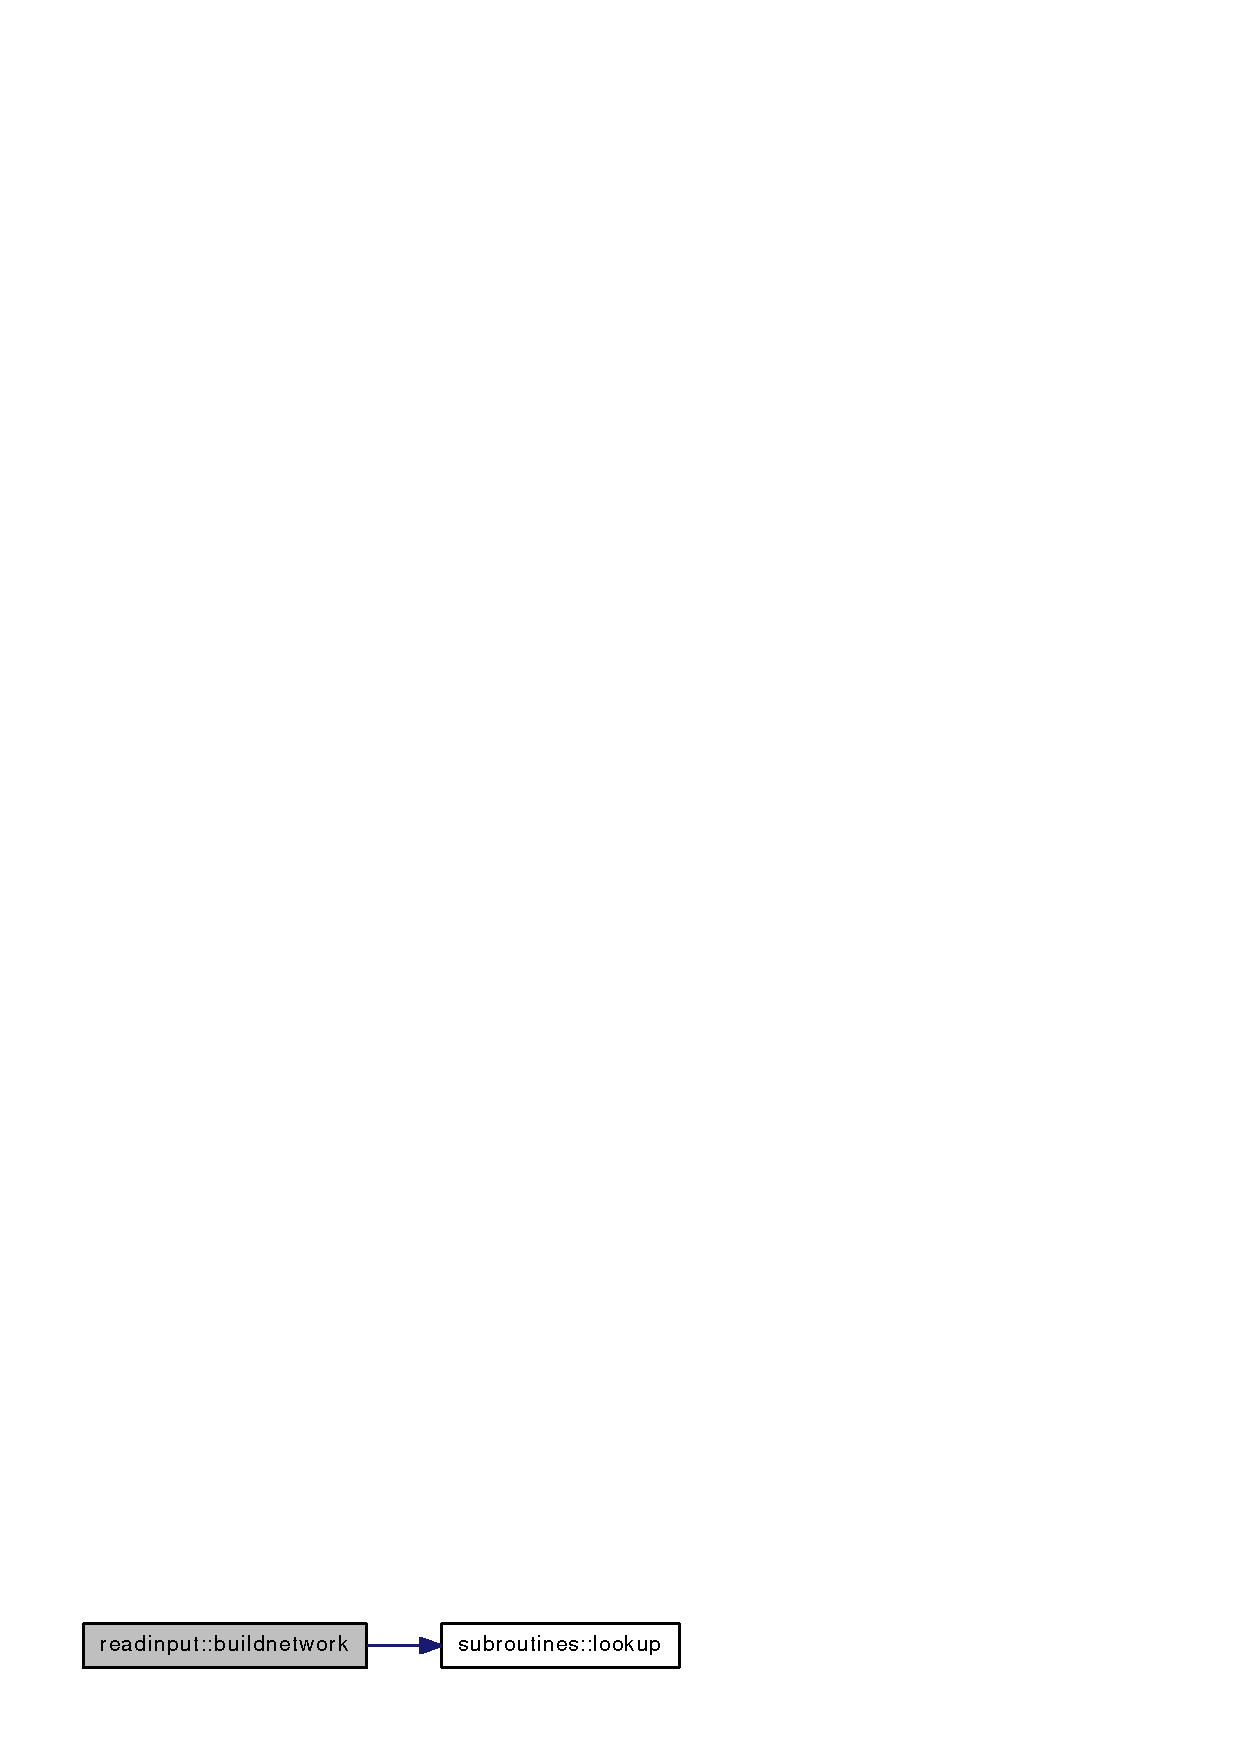
\includegraphics[width=165pt]{namespacereadinput_a29790780c02003cbcba39bb214e7ffd0_cgraph}
\end{center}
\end{figure}


Here is the caller graph for this function:\nopagebreak
\begin{figure}[H]
\begin{center}
\leavevmode
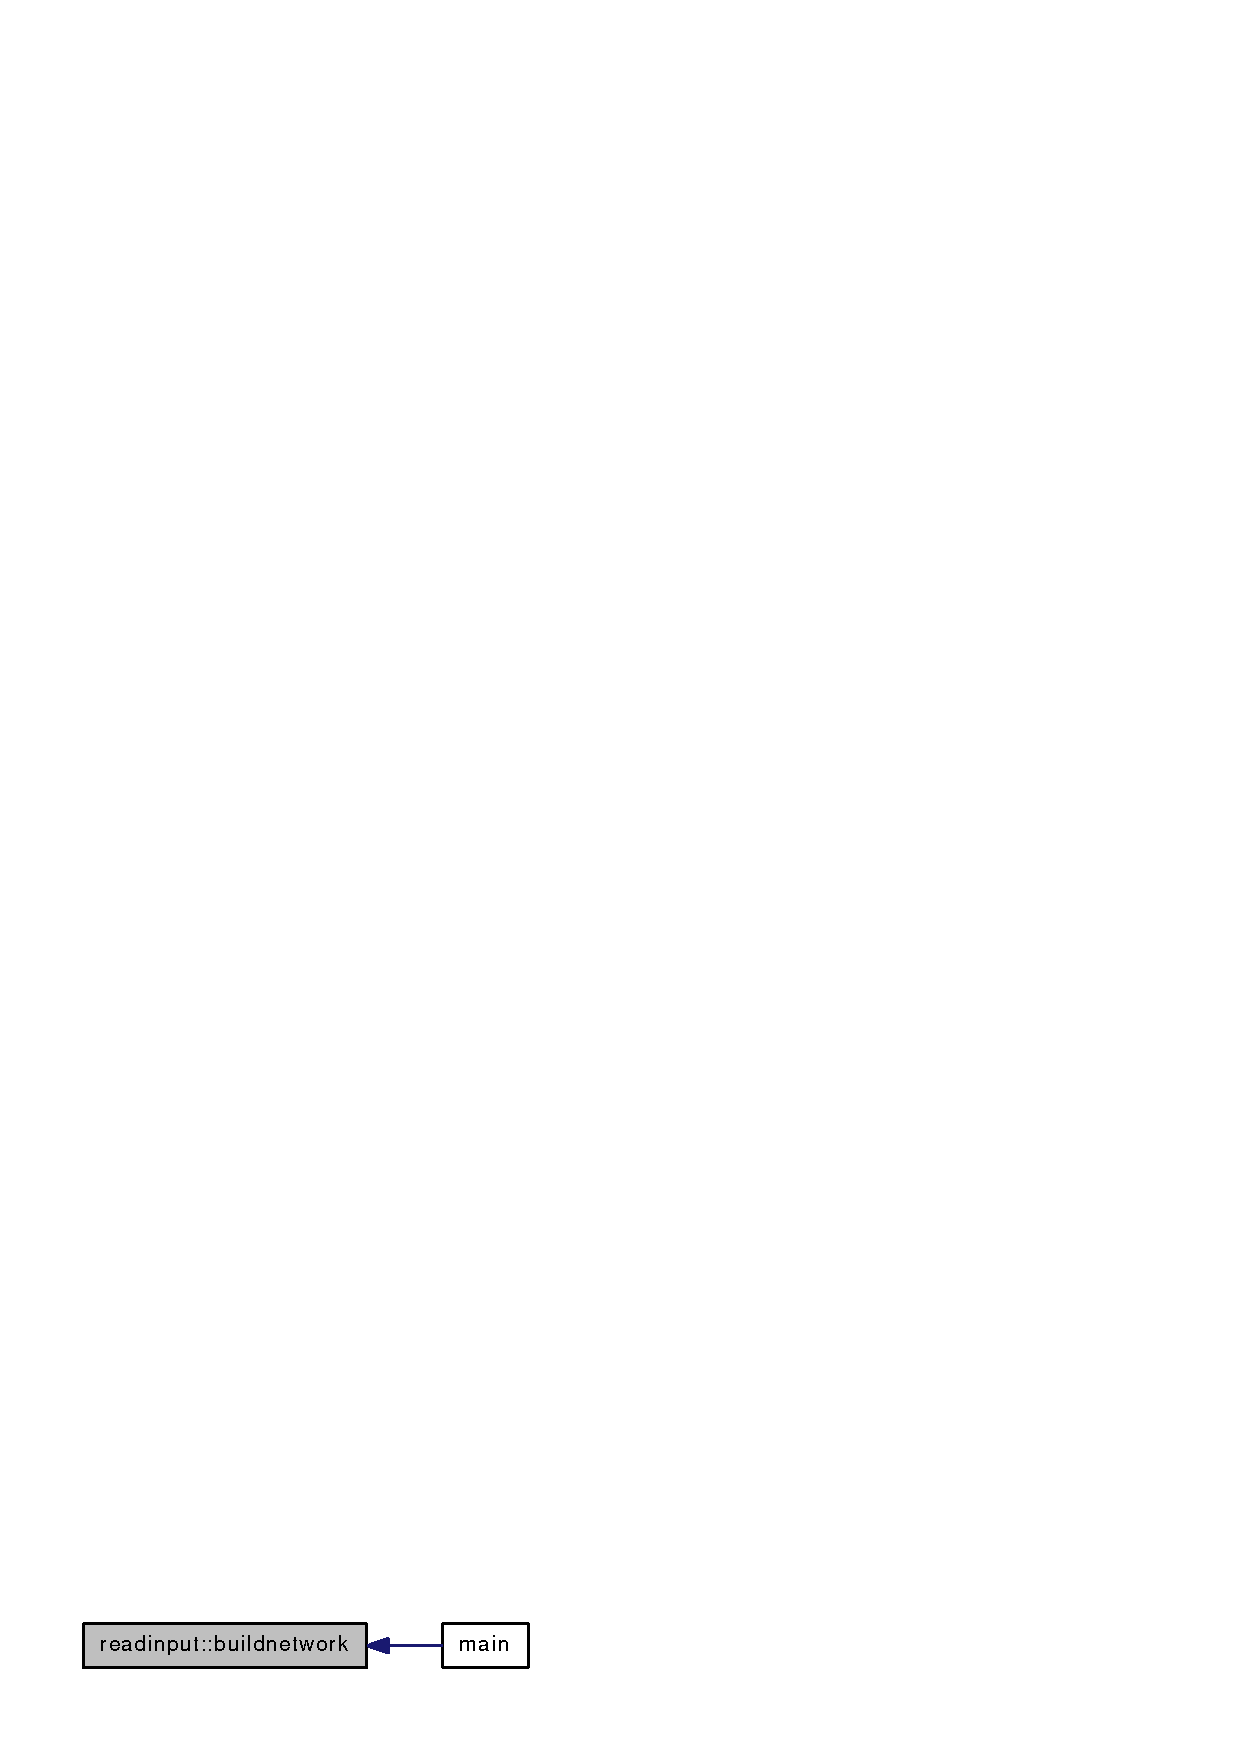
\includegraphics[width=129pt]{namespacereadinput_a29790780c02003cbcba39bb214e7ffd0_icgraph}
\end{center}
\end{figure}

\hypertarget{namespacespecdata}{
\section{specdata Module Reference}
\label{namespacespecdata}\index{specdata@{specdata}}
}
\subsection*{Variables}
\begin{DoxyCompactItemize}
\item 
TYPE(EPG\_\-EXSTATE), dimension(5), parameter \hyperlink{namespacespecdata_ae681c0bc4ab2fa5470a5956b4bec78d0}{o2\_\-p\_\-ex} = (/ EPG\_\-EXSTATE( ,0.092,2.50,0.5,3.0 ,0.98), EPG\_\-EXSTATE(,0.109,4.19,0.5,3.0 ,1.64), EPG\_\-EXSTATE(,0.57 ,17.6,0.5,0.9 ,4.5) , EPG\_\-EXSTATE(,4.73 ,51.7,0.5,0.75,8.4) , EPG\_\-EXSTATE( ,0.83 ,80.7,0.5,0.85,9.9) /)
\item 
TYPE(EPG\_\-EXSTATE), dimension(4), parameter \hyperlink{namespacespecdata_ae83fc5fae3d6873e5453849a6289952f}{o\_\-p\_\-ex} = (/ EPG\_\-EXSTATE(,0.51 ,5.4 ,1.0,1.0,1.85), EPG\_\-EXSTATE(,0.075,8.7 ,1.0,1.0,4.18), EPG\_\-EXSTATE(,0.38 ,37.2,1.0,1.0,9.53), EPG\_\-EXSTATE(,0.55 ,16.1,1.0,1.0,9.20) /)
\item 
TYPE(EPG\_\-EXSTATE), dimension(1), parameter \hyperlink{namespacespecdata_a5715afaf9a7cd31ff6c899aec265dc7e}{o3\_\-p\_\-ex} = (/ EPG\_\-EXSTATE(, 1.0, 20.00, 1.0, 2.5, 4.9) /)
\item 
TYPE(EPG\_\-IONSTATE), dimension(7), parameter \hyperlink{namespacespecdata_a1de88d1ad1d0aa421deaf2c5ac887ed8}{o2\_\-p\_\-ion} = (/ EPG\_\-IONSTATE(,9.56D0,45.8,0.61D0,1.26D0,12.1D0) , EPG\_\-IONSTATE(,5.38D0,127.1,1.1D0,0.58D0,16.1D0) , EPG\_\-IONSTATE(,5.25D0,170.3,1.1D0,0.60D0,16.9D0) , EPG\_\-IONSTATE(,3.19D0,142.4,1.1D0,0.58D0,18.2D0), EPG\_\-IONSTATE(,0.94D0,140.8,1.1D0,0.58D0,23.0D0) , EPG\_\-IONSTATE(,15.6D0,56.0,1.2D0,0.72D0,18.0D0) , EPG\_\-IONSTATE(,8.75D0,57.0,1.2D0,0.72D0,22.0D0) /)
\item 
TYPE(EPG\_\-IONSTATE), dimension(3), parameter \hyperlink{namespacespecdata_a67659f2839588aff464762d181bccdd7}{o\_\-p\_\-ion} = (/ EPG\_\-IONSTATE(,20.4,61.5,0.82,0.75,13.6), EPG\_\-IONSTATE(,25.4,69.5,0.82,0.75,16.9), EPG\_\-IONSTATE(,10.8,72.8,0.82,0.75,18.5) /)
\item 
TYPE(EPG\_\-IONSTATE), dimension(1), parameter \hyperlink{namespacespecdata_a42d18c80256a5ca2ccebe8a3f4d451a0}{o3\_\-p\_\-ion} = (/ EPG\_\-IONSTATE(, 40.00, 105.00, 1.00, 0.75, 12.43 ) /)
\item 
TYPE(ALWD\_\-EXSTATE), dimension(2), parameter \hyperlink{namespacespecdata_accca75874b57e169b91c0b680bffd51f}{o2\_\-e\_\-ex\_\-alwd} = (/ ALWD\_\-EXSTATE(,8.4,0.254,0.037,1.19,2.31), ALWD\_\-EXSTATE(,9.9,0.0285,0.622,1.38,3.44) /)
\item 
TYPE(FBDN\_\-EXSTATE), dimension(3), parameter \hyperlink{namespacespecdata_af2d6b8fc566715d79d76b79cc900229e}{o2\_\-e\_\-ex\_\-fbdn} = (/ FBDN\_\-EXSTATE(,1.64,0.0005,3.0,3.0,1.0) , FBDN\_\-EXSTATE(,0.98,0.0005,3.0,3.0,1.0) , FBDN\_\-EXSTATE(,4.5,0.021,0.9,1.0,1.0) /)
\item 
TYPE(ALWD\_\-EXSTATE), dimension(2), parameter \hyperlink{namespacespecdata_ac6de9abf8a4350031cdeed967f2b21b6}{o\_\-e\_\-ex\_\-alwd} = (/ ALWD\_\-EXSTATE(,9.53,0.0560,0.320,0.86,1.440), ALWD\_\-EXSTATE(,12.10,0.0310,0.610,1.26,0.490) /)
\item 
TYPE(FBDN\_\-EXSTATE), dimension(2), parameter \hyperlink{namespacespecdata_a31f902ca9efd2ca7817a66af34743c3d}{o\_\-e\_\-ex\_\-fbdn} = (/ FBDN\_\-EXSTATE(,1.85,0.0100,1.000,1.00,2.00) , FBDN\_\-EXSTATE(,4.18,0.0042,1.00,0.50,1.000) /)
\item 
TYPE(IONSTATE), dimension(1), parameter \hyperlink{namespacespecdata_a7040a4bcf92d1e17f6158536ca8d5b0a}{o2\_\-e\_\-ion} = (/ IONSTATE(,12.1,0.475,0.0,3.760,0.0,0.0,18.50,12.10,1.860,1000.0,24.20) /)
\item 
TYPE(IONSTATE), dimension(1), parameter \hyperlink{namespacespecdata_aa92d120444752fc22443b31d087da308}{o\_\-e\_\-ion} = (/ IONSTATE(,13.6,1.03,0.0,1.81,0.0,0.0,13.0,-\/0.815,6.41,3450.0,162.0) /)
\end{DoxyCompactItemize}


\subsection{Variable Documentation}
\hypertarget{namespacespecdata_accca75874b57e169b91c0b680bffd51f}{
\index{specdata@{specdata}!o2\_\-e\_\-ex\_\-alwd@{o2\_\-e\_\-ex\_\-alwd}}
\index{o2\_\-e\_\-ex\_\-alwd@{o2\_\-e\_\-ex\_\-alwd}!specdata@{specdata}}
\subsubsection[{o2\_\-e\_\-ex\_\-alwd}]{\setlength{\rightskip}{0pt plus 5cm}TYPE(ALWD\_\-EXSTATE),dimension(2),parameter {\bf specdata::o2\_\-e\_\-ex\_\-alwd} = (/ ALWD\_\-EXSTATE(,8.4,0.254,0.037,1.19,2.31), ALWD\_\-EXSTATE(,9.9,0.0285,0.622,1.38,3.44) /)}}
\label{namespacespecdata_accca75874b57e169b91c0b680bffd51f}


Definition at line 60 of file specdata.f90.

Referenced by subroutines::esigma\_\-suite(), and subroutines::se\_\-info\_\-init().\hypertarget{namespacespecdata_af2d6b8fc566715d79d76b79cc900229e}{
\index{specdata@{specdata}!o2\_\-e\_\-ex\_\-fbdn@{o2\_\-e\_\-ex\_\-fbdn}}
\index{o2\_\-e\_\-ex\_\-fbdn@{o2\_\-e\_\-ex\_\-fbdn}!specdata@{specdata}}
\subsubsection[{o2\_\-e\_\-ex\_\-fbdn}]{\setlength{\rightskip}{0pt plus 5cm}TYPE(FBDN\_\-EXSTATE),dimension(3),parameter {\bf specdata::o2\_\-e\_\-ex\_\-fbdn} = (/ FBDN\_\-EXSTATE(,1.64,0.0005,3.0,3.0,1.0) , FBDN\_\-EXSTATE(,0.98,0.0005,3.0,3.0,1.0) , FBDN\_\-EXSTATE(,4.5,0.021,0.9,1.0,1.0) /)}}
\label{namespacespecdata_af2d6b8fc566715d79d76b79cc900229e}


Definition at line 70 of file specdata.f90.

Referenced by subroutines::esigma\_\-suite(), and subroutines::se\_\-info\_\-init().\hypertarget{namespacespecdata_a7040a4bcf92d1e17f6158536ca8d5b0a}{
\index{specdata@{specdata}!o2\_\-e\_\-ion@{o2\_\-e\_\-ion}}
\index{o2\_\-e\_\-ion@{o2\_\-e\_\-ion}!specdata@{specdata}}
\subsubsection[{o2\_\-e\_\-ion}]{\setlength{\rightskip}{0pt plus 5cm}TYPE(IONSTATE),dimension(1),parameter {\bf specdata::o2\_\-e\_\-ion} = (/ IONSTATE(,12.1,0.475,0.0,3.760,0.0,0.0,18.50,12.10,1.860,1000.0,24.20) /)}}
\label{namespacespecdata_a7040a4bcf92d1e17f6158536ca8d5b0a}


Definition at line 98 of file specdata.f90.

Referenced by subroutines::se\_\-info\_\-init().\hypertarget{namespacespecdata_ae681c0bc4ab2fa5470a5956b4bec78d0}{
\index{specdata@{specdata}!o2\_\-p\_\-ex@{o2\_\-p\_\-ex}}
\index{o2\_\-p\_\-ex@{o2\_\-p\_\-ex}!specdata@{specdata}}
\subsubsection[{o2\_\-p\_\-ex}]{\setlength{\rightskip}{0pt plus 5cm}TYPE(EPG\_\-EXSTATE),dimension(5),parameter {\bf specdata::o2\_\-p\_\-ex} = (/ EPG\_\-EXSTATE( ,0.092,2.50,0.5,3.0 ,0.98), EPG\_\-EXSTATE(,0.109,4.19,0.5,3.0 ,1.64), EPG\_\-EXSTATE(,0.57 ,17.6,0.5,0.9 ,4.5) , EPG\_\-EXSTATE(,4.73 ,51.7,0.5,0.75,8.4) , EPG\_\-EXSTATE( ,0.83 ,80.7,0.5,0.85,9.9) /)}}
\label{namespacespecdata_ae681c0bc4ab2fa5470a5956b4bec78d0}


Definition at line 9 of file specdata.f90.

Referenced by subroutines::fallout(), subroutines::p\_\-ex\_\-select(), subroutines::psigma\_\-suite(), and sigma\_\-test().\hypertarget{namespacespecdata_a1de88d1ad1d0aa421deaf2c5ac887ed8}{
\index{specdata@{specdata}!o2\_\-p\_\-ion@{o2\_\-p\_\-ion}}
\index{o2\_\-p\_\-ion@{o2\_\-p\_\-ion}!specdata@{specdata}}
\subsubsection[{o2\_\-p\_\-ion}]{\setlength{\rightskip}{0pt plus 5cm}TYPE(EPG\_\-IONSTATE),dimension(7),parameter {\bf specdata::o2\_\-p\_\-ion} = (/ EPG\_\-IONSTATE(,9.56D0,45.8,0.61D0,1.26D0,12.1D0) , EPG\_\-IONSTATE(,5.38D0,127.1,1.1D0,0.58D0,16.1D0) , EPG\_\-IONSTATE(,5.25D0,170.3,1.1D0,0.60D0,16.9D0) , EPG\_\-IONSTATE(,3.19D0,142.4,1.1D0,0.58D0,18.2D0), EPG\_\-IONSTATE(,0.94D0,140.8,1.1D0,0.58D0,23.0D0) , EPG\_\-IONSTATE(,15.6D0,56.0,1.2D0,0.72D0,18.0D0) , EPG\_\-IONSTATE(,8.75D0,57.0,1.2D0,0.72D0,22.0D0) /)}}
\label{namespacespecdata_a1de88d1ad1d0aa421deaf2c5ac887ed8}


Definition at line 33 of file specdata.f90.

Referenced by subroutines::fallout(), subroutines::p\_\-ion\_\-select(), subroutines::psigma\_\-suite(), and sigma\_\-test().\hypertarget{namespacespecdata_a5715afaf9a7cd31ff6c899aec265dc7e}{
\index{specdata@{specdata}!o3\_\-p\_\-ex@{o3\_\-p\_\-ex}}
\index{o3\_\-p\_\-ex@{o3\_\-p\_\-ex}!specdata@{specdata}}
\subsubsection[{o3\_\-p\_\-ex}]{\setlength{\rightskip}{0pt plus 5cm}TYPE(EPG\_\-EXSTATE),dimension(1),parameter {\bf specdata::o3\_\-p\_\-ex} = (/ EPG\_\-EXSTATE(, 1.0, 20.00, 1.0, 2.5, 4.9) /)}}
\label{namespacespecdata_a5715afaf9a7cd31ff6c899aec265dc7e}


Definition at line 28 of file specdata.f90.

Referenced by subroutines::e\_\-ex\_\-select(), subroutines::esigma\_\-suite(), subroutines::fallout(), subroutines::p\_\-ex\_\-select(), subroutines::psigma\_\-suite(), and sigma\_\-test().\hypertarget{namespacespecdata_a42d18c80256a5ca2ccebe8a3f4d451a0}{
\index{specdata@{specdata}!o3\_\-p\_\-ion@{o3\_\-p\_\-ion}}
\index{o3\_\-p\_\-ion@{o3\_\-p\_\-ion}!specdata@{specdata}}
\subsubsection[{o3\_\-p\_\-ion}]{\setlength{\rightskip}{0pt plus 5cm}TYPE(EPG\_\-IONSTATE),dimension(1),parameter {\bf specdata::o3\_\-p\_\-ion} = (/ EPG\_\-IONSTATE(, 40.00, 105.00, 1.00, 0.75, 12.43 ) /)}}
\label{namespacespecdata_a42d18c80256a5ca2ccebe8a3f4d451a0}


Definition at line 52 of file specdata.f90.

Referenced by subroutines::e\_\-ion\_\-select(), subroutines::esigma\_\-suite(), subroutines::fallout(), subroutines::p\_\-ion\_\-select(), subroutines::psigma\_\-suite(), and sigma\_\-test().\hypertarget{namespacespecdata_ac6de9abf8a4350031cdeed967f2b21b6}{
\index{specdata@{specdata}!o\_\-e\_\-ex\_\-alwd@{o\_\-e\_\-ex\_\-alwd}}
\index{o\_\-e\_\-ex\_\-alwd@{o\_\-e\_\-ex\_\-alwd}!specdata@{specdata}}
\subsubsection[{o\_\-e\_\-ex\_\-alwd}]{\setlength{\rightskip}{0pt plus 5cm}TYPE(ALWD\_\-EXSTATE),dimension(2),parameter {\bf specdata::o\_\-e\_\-ex\_\-alwd} = (/ ALWD\_\-EXSTATE(,9.53,0.0560,0.320,0.86,1.440), ALWD\_\-EXSTATE(,12.10,0.0310,0.610,1.26,0.490) /)}}
\label{namespacespecdata_ac6de9abf8a4350031cdeed967f2b21b6}


Definition at line 81 of file specdata.f90.

Referenced by subroutines::esigma\_\-suite(), and subroutines::se\_\-info\_\-init().\hypertarget{namespacespecdata_a31f902ca9efd2ca7817a66af34743c3d}{
\index{specdata@{specdata}!o\_\-e\_\-ex\_\-fbdn@{o\_\-e\_\-ex\_\-fbdn}}
\index{o\_\-e\_\-ex\_\-fbdn@{o\_\-e\_\-ex\_\-fbdn}!specdata@{specdata}}
\subsubsection[{o\_\-e\_\-ex\_\-fbdn}]{\setlength{\rightskip}{0pt plus 5cm}TYPE(FBDN\_\-EXSTATE),dimension(2),parameter {\bf specdata::o\_\-e\_\-ex\_\-fbdn} = (/ FBDN\_\-EXSTATE(,1.85,0.0100,1.000,1.00,2.00) , FBDN\_\-EXSTATE(,4.18,0.0042,1.00,0.50,1.000) /)}}
\label{namespacespecdata_a31f902ca9efd2ca7817a66af34743c3d}


Definition at line 91 of file specdata.f90.

Referenced by subroutines::esigma\_\-suite(), and subroutines::se\_\-info\_\-init().\hypertarget{namespacespecdata_aa92d120444752fc22443b31d087da308}{
\index{specdata@{specdata}!o\_\-e\_\-ion@{o\_\-e\_\-ion}}
\index{o\_\-e\_\-ion@{o\_\-e\_\-ion}!specdata@{specdata}}
\subsubsection[{o\_\-e\_\-ion}]{\setlength{\rightskip}{0pt plus 5cm}TYPE(IONSTATE),dimension(1),parameter {\bf specdata::o\_\-e\_\-ion} = (/ IONSTATE(,13.6,1.03,0.0,1.81,0.0,0.0,13.0,-\/0.815,6.41,3450.0,162.0) /)}}
\label{namespacespecdata_aa92d120444752fc22443b31d087da308}


Definition at line 103 of file specdata.f90.

Referenced by subroutines::se\_\-info\_\-init().\hypertarget{namespacespecdata_ae83fc5fae3d6873e5453849a6289952f}{
\index{specdata@{specdata}!o\_\-p\_\-ex@{o\_\-p\_\-ex}}
\index{o\_\-p\_\-ex@{o\_\-p\_\-ex}!specdata@{specdata}}
\subsubsection[{o\_\-p\_\-ex}]{\setlength{\rightskip}{0pt plus 5cm}TYPE(EPG\_\-EXSTATE),dimension(4),parameter {\bf specdata::o\_\-p\_\-ex} = (/ EPG\_\-EXSTATE(,0.51 ,5.4 ,1.0,1.0,1.85), EPG\_\-EXSTATE(,0.075,8.7 ,1.0,1.0,4.18), EPG\_\-EXSTATE(,0.38 ,37.2,1.0,1.0,9.53), EPG\_\-EXSTATE(,0.55 ,16.1,1.0,1.0,9.20) /)}}
\label{namespacespecdata_ae83fc5fae3d6873e5453849a6289952f}


Definition at line 19 of file specdata.f90.

Referenced by subroutines::fallout(), subroutines::p\_\-ex\_\-select(), subroutines::psigma\_\-suite(), and sigma\_\-test().\hypertarget{namespacespecdata_a67659f2839588aff464762d181bccdd7}{
\index{specdata@{specdata}!o\_\-p\_\-ion@{o\_\-p\_\-ion}}
\index{o\_\-p\_\-ion@{o\_\-p\_\-ion}!specdata@{specdata}}
\subsubsection[{o\_\-p\_\-ion}]{\setlength{\rightskip}{0pt plus 5cm}TYPE(EPG\_\-IONSTATE),dimension(3),parameter {\bf specdata::o\_\-p\_\-ion} = (/ EPG\_\-IONSTATE(,20.4,61.5,0.82,0.75,13.6), EPG\_\-IONSTATE(,25.4,69.5,0.82,0.75,16.9), EPG\_\-IONSTATE(,10.8,72.8,0.82,0.75,18.5) /)}}
\label{namespacespecdata_a67659f2839588aff464762d181bccdd7}


Definition at line 45 of file specdata.f90.

Referenced by subroutines::fallout(), subroutines::p\_\-ion\_\-select(), subroutines::psigma\_\-suite(), and sigma\_\-test().
\hypertarget{namespacesubroutines}{
\section{subroutines Module Reference}
\label{namespacesubroutines}\index{subroutines@{subroutines}}
}
\subsection*{Functions/Subroutines}
\begin{DoxyCompactItemize}
\item 
subroutine \hyperlink{namespacesubroutines_a27505ee5071c93bb5f1e570995a1ac42}{lookup} (name, \hyperlink{typetypedefs_1_1node}{node}, id, atoms, charge)
\item 
subroutine \hyperlink{namespacesubroutines_a0ce9ee9331d3c0bba11e3e00fbd7e07b}{writereactions} (\hyperlink{typetypedefs_1_1node}{node})
\item 
subroutine \hyperlink{namespacesubroutines_ad97e0b9db9cfe6329f9f8fdb886077e7}{hopping} (i\_\-in, j\_\-in, k\_\-in, i\_\-out, j\_\-out, k\_\-out, prob)
\item 
subroutine \hyperlink{namespacesubroutines_a7a31d5c9fbda24651c932b0466618567}{fallout} (root, temp, prevNode, nextNode)
\item 
subroutine \hyperlink{namespacesubroutines_af4c69699bd3e0e4aa05607a7e94044dc}{find\_\-empty\_\-site} (in\_\-coords, out\_\-coords, null)
\item 
subroutine \hyperlink{namespacesubroutines_ac847bd99eab89bdc881d885b2808624d}{wait\_\-calc} (temp)
\item 
subroutine \hyperlink{namespacesubroutines_af250b65cb2805243dd52e4e3535f4c5a}{counter} ()
\item 
subroutine \hyperlink{namespacesubroutines_a0a51843cbd2415487f29e4314e1de97a}{transport} (prev, curr, next)
\item 
subroutine \hyperlink{namespacesubroutines_a37b9d3b519b164f5ef3835bf4e1e4f8c}{psigma\_\-suite} (energy, psigmas, psigij, psigexj, o\_\-psigmas, o\_\-psigij, o\_\-psigexj, o3\_\-psigmas, o3\_\-psigij, o3\_\-psigexj)
\item 
subroutine \hyperlink{namespacesubroutines_a27620c6392f4cd49238c295cbe60e179}{esigma\_\-suite} (se\_\-box)
\item 
subroutine \hyperlink{namespacesubroutines_a3185cd857374fa3b0a19f2a56e6474df}{p\_\-ion\_\-select} (psigij, e\_\-ion, e\_\-se, thinghit)
\item 
subroutine \hyperlink{namespacesubroutines_acad706394e0b01bbd1e5345585dace59}{p\_\-ex\_\-select} (psigexj, e\_\-exc, thinghit)
\item 
subroutine \hyperlink{namespacesubroutines_acad777e3f27acb4f7e0f7b35035ae54a}{e\_\-ion\_\-select} (se\_\-box, e\_\-ion, e\_\-se, null, thinghit)
\item 
subroutine \hyperlink{namespacesubroutines_a0f09eb60b63730612ddd7801066ce49b}{e\_\-ex\_\-select} (se\_\-box, e\_\-exc, null, thinghit)
\item 
subroutine \hyperlink{namespacesubroutines_a10f3c575d44eedaf9b0a95ed9a64e3ab}{elastic\_\-event} (energy, e\_\-loss, labtheta)
\item 
subroutine \hyperlink{namespacesubroutines_aece587c9d144811189bd1ccf8a59f189}{se\_\-info\_\-init} (se\_\-box)
\item 
subroutine \hyperlink{namespacesubroutines_a1d1775ee81394d8c078c760678a530e2}{se\_\-info\_\-garbage} (se\_\-box)
\item 
subroutine \hyperlink{namespacesubroutines_a4d9b1fbbdcfc2b420201a7ca71c4e782}{init\_\-node} (root, temp\_\-node, x, y, z)
\item 
subroutine \hyperlink{namespacesubroutines_a7580fc0416f20d44b3cfa79ebc20a839}{wipe\_\-node} (x, y, z)
\item 
subroutine \hyperlink{namespacesubroutines_a5f9a688681311ebc691561ec51015d0f}{new\_\-reaction} (i, j, k, root, temp, prevNode, nextNode, error)
\item 
subroutine \hyperlink{namespacesubroutines_ae942148085820c335aea6798ad4e7e7e}{new\_\-electron} (se\_\-box, root, temp, prevNode, nextNode)
\item 
subroutine \hyperlink{namespacesubroutines_aae3cb4fad8f95b0869777449a6bc496f}{analyzereaction} (reactnode, speciesnum, yield, nature)
\item 
subroutine \hyperlink{namespacesubroutines_abbce0f7ec92c43ac91db25f512531642}{trackwrite} (coords, energy, e\_\-branch, electron)
\end{DoxyCompactItemize}


\subsection{Function/Subroutine Documentation}
\hypertarget{namespacesubroutines_aae3cb4fad8f95b0869777449a6bc496f}{
\index{subroutines@{subroutines}!analyzereaction@{analyzereaction}}
\index{analyzereaction@{analyzereaction}!subroutines@{subroutines}}
\subsubsection[{analyzereaction}]{\setlength{\rightskip}{0pt plus 5cm}subroutine subroutines::analyzereaction (TYPE (reaction) {\em reactnode}, \/  integer,intent(in) {\em speciesnum}, \/  integer,intent(out) {\em yield}, \/  character(30),intent(out) {\em nature})}}
\label{namespacesubroutines_aae3cb4fad8f95b0869777449a6bc496f}


Definition at line 2461 of file subroutines.f90.

Referenced by writereactions().

Here is the caller graph for this function:\nopagebreak
\begin{figure}[H]
\begin{center}
\leavevmode
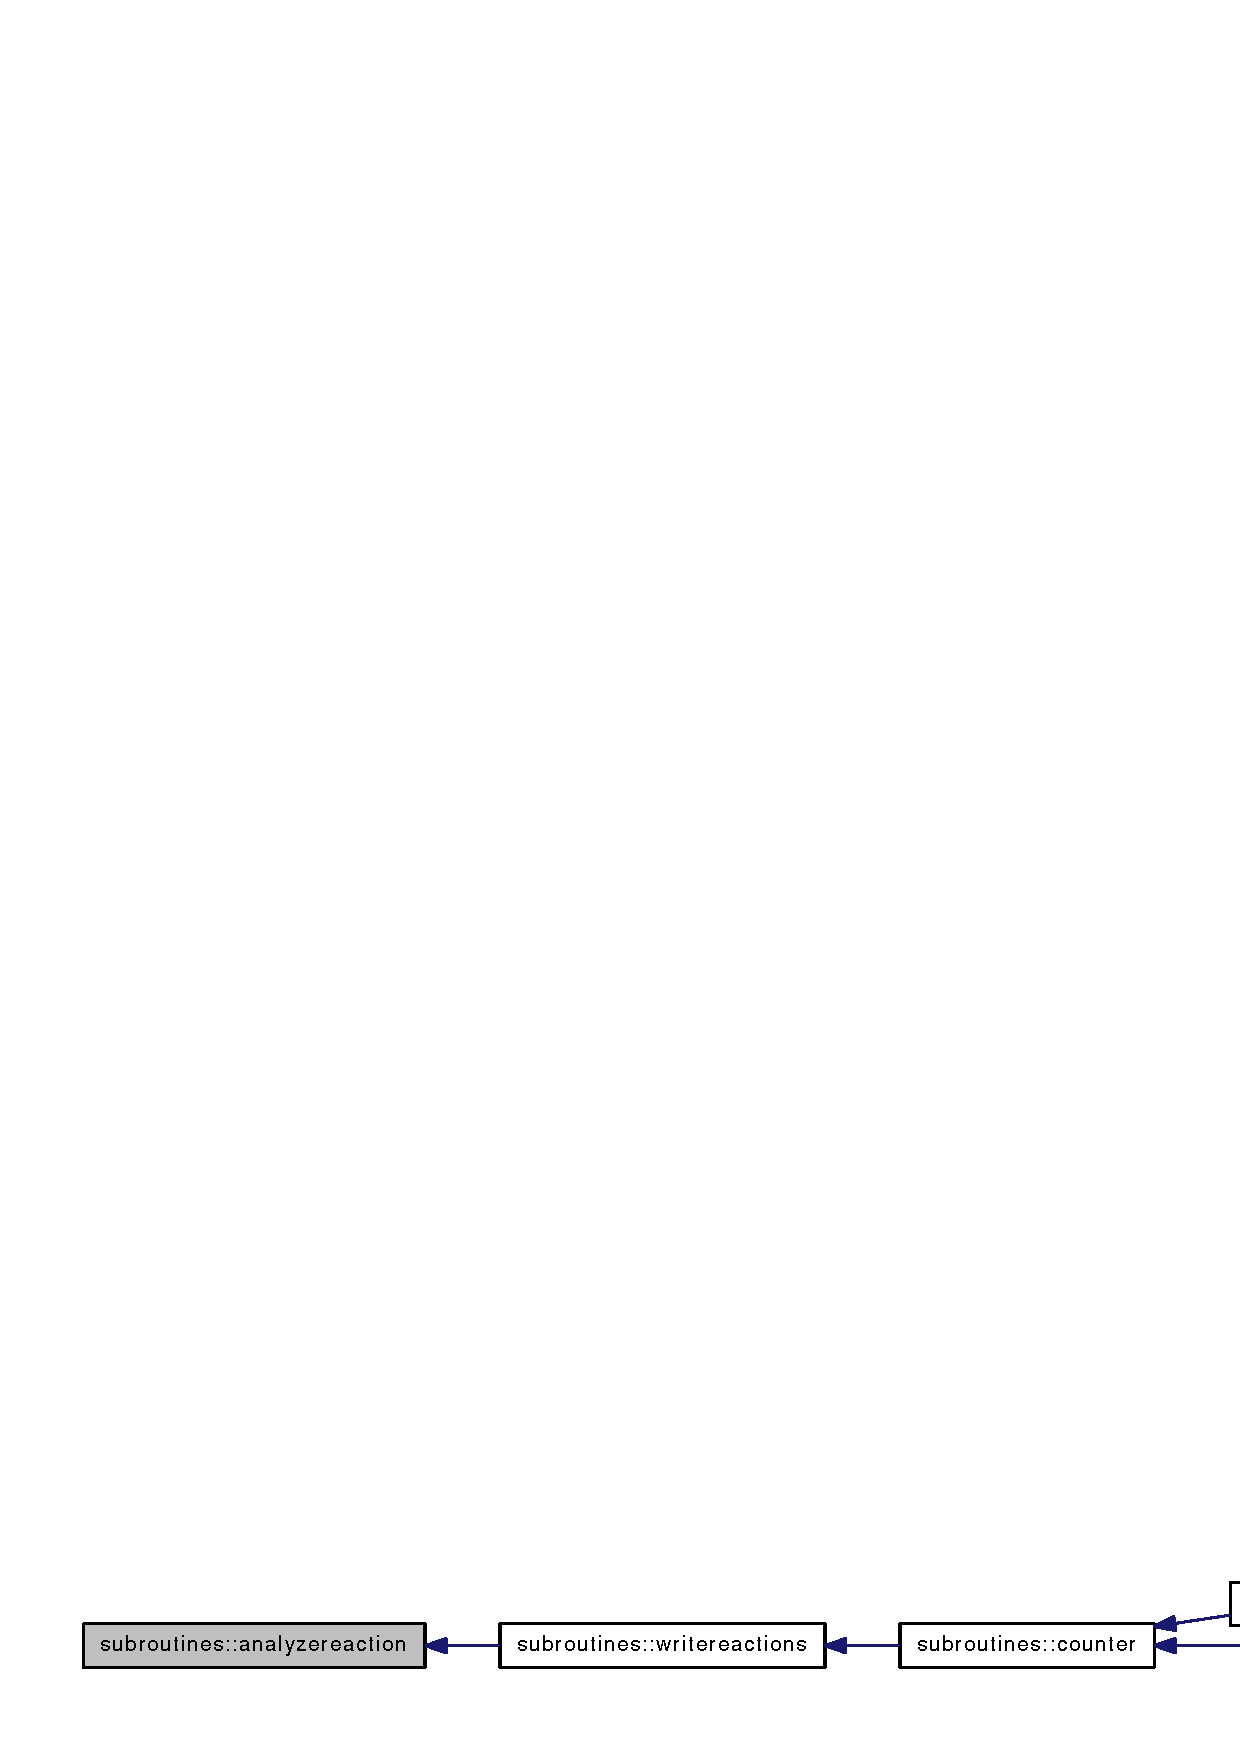
\includegraphics[width=372pt]{namespacesubroutines_aae3cb4fad8f95b0869777449a6bc496f_icgraph}
\end{center}
\end{figure}
\hypertarget{namespacesubroutines_af250b65cb2805243dd52e4e3535f4c5a}{
\index{subroutines@{subroutines}!counter@{counter}}
\index{counter@{counter}!subroutines@{subroutines}}
\subsubsection[{counter}]{\setlength{\rightskip}{0pt plus 5cm}subroutine subroutines::counter ()}}
\label{namespacesubroutines_af250b65cb2805243dd52e4e3535f4c5a}


Definition at line 854 of file subroutines.f90.

References parameters::AB\_\-LUN, parameters::CUIRCT, parameters::DIMENS, parameters::EDGE, parameters::FLUENCE, parameters::GEMINACY\_\-LUN, parameters::GVALUE, parameters::initialatoms, parameters::MATRIX, parameters::NO\_\-OUTPUT, parameters::O2\_\-ABUNDANCE, parameters::O2NUM, parameters::O2STARNUM, parameters::O3\_\-ABUNDANCE, parameters::O3NUM, parameters::O3STARNUM, parameters::O\_\-ABUNDANCE, parameters::ONUM, parameters::OSTARNUM, parameters::QUIET, parameters::RE\_\-HEAD, parameters::SP\_\-PROD\_\-DEST, parameters::THICK, parameters::TIME, parameters::TOTAL\_\-PROTON\_\-ELOSS, and writereactions().

Referenced by gp::fitness(), and main().

Here is the call graph for this function:\nopagebreak
\begin{figure}[H]
\begin{center}
\leavevmode
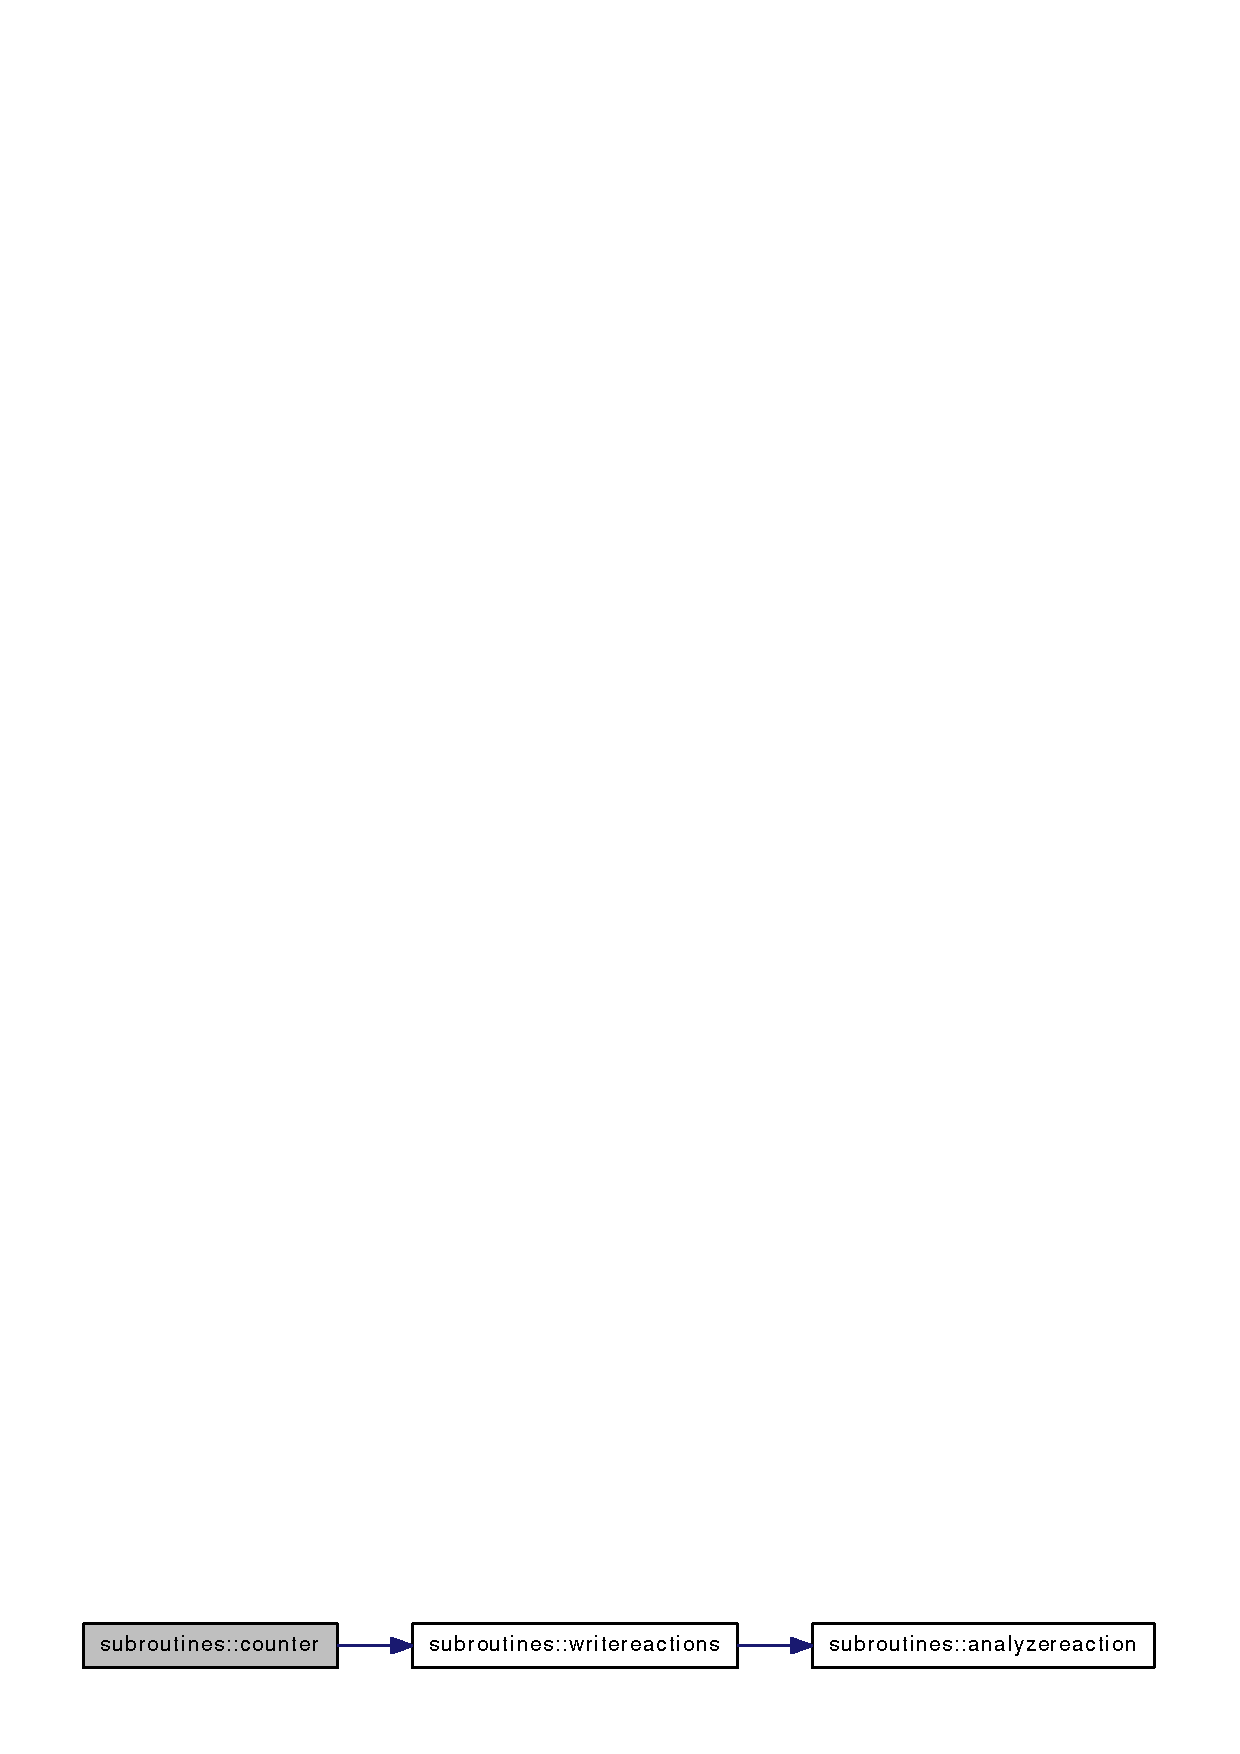
\includegraphics[width=279pt]{namespacesubroutines_af250b65cb2805243dd52e4e3535f4c5a_cgraph}
\end{center}
\end{figure}


Here is the caller graph for this function:\nopagebreak
\begin{figure}[H]
\begin{center}
\leavevmode
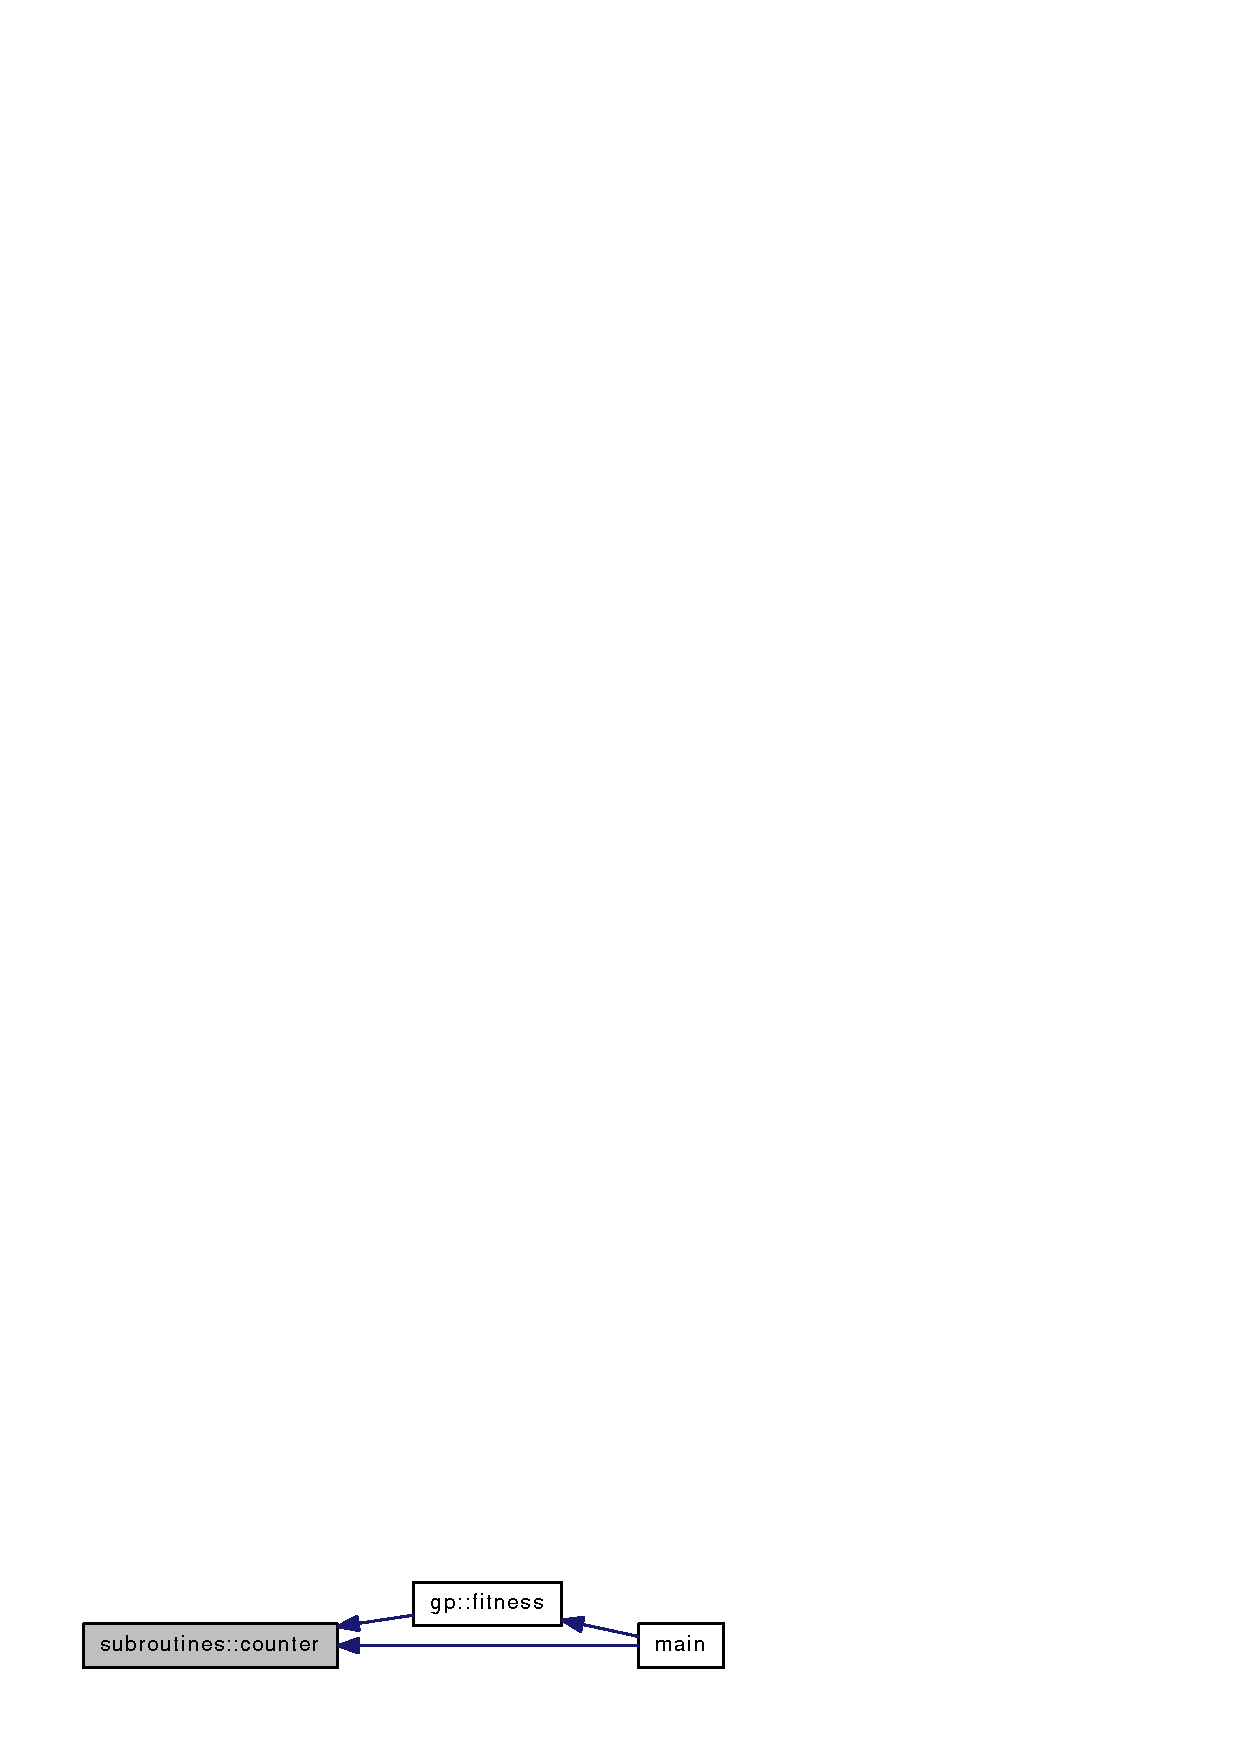
\includegraphics[width=176pt]{namespacesubroutines_af250b65cb2805243dd52e4e3535f4c5a_icgraph}
\end{center}
\end{figure}
\hypertarget{namespacesubroutines_a0f09eb60b63730612ddd7801066ce49b}{
\index{subroutines@{subroutines}!e\_\-ex\_\-select@{e\_\-ex\_\-select}}
\index{e\_\-ex\_\-select@{e\_\-ex\_\-select}!subroutines@{subroutines}}
\subsubsection[{e\_\-ex\_\-select}]{\setlength{\rightskip}{0pt plus 5cm}subroutine subroutines::e\_\-ex\_\-select (TYPE(se\_\-info) {\em se\_\-box}, \/  DOUBLE PRECISION,intent(out) {\em e\_\-exc}, \/  INTEGER,intent(out) {\em null}, \/  INTEGER,intent(in) {\em thinghit})}}
\label{namespacesubroutines_a0f09eb60b63730612ddd7801066ce49b}


Definition at line 1722 of file subroutines.f90.

References specdata::o3\_\-p\_\-ex, parameters::O3NUM, parameters::O3STARNUM, parameters::ONUM, and parameters::OSTARNUM.

Referenced by new\_\-electron().

Here is the caller graph for this function:\nopagebreak
\begin{figure}[H]
\begin{center}
\leavevmode
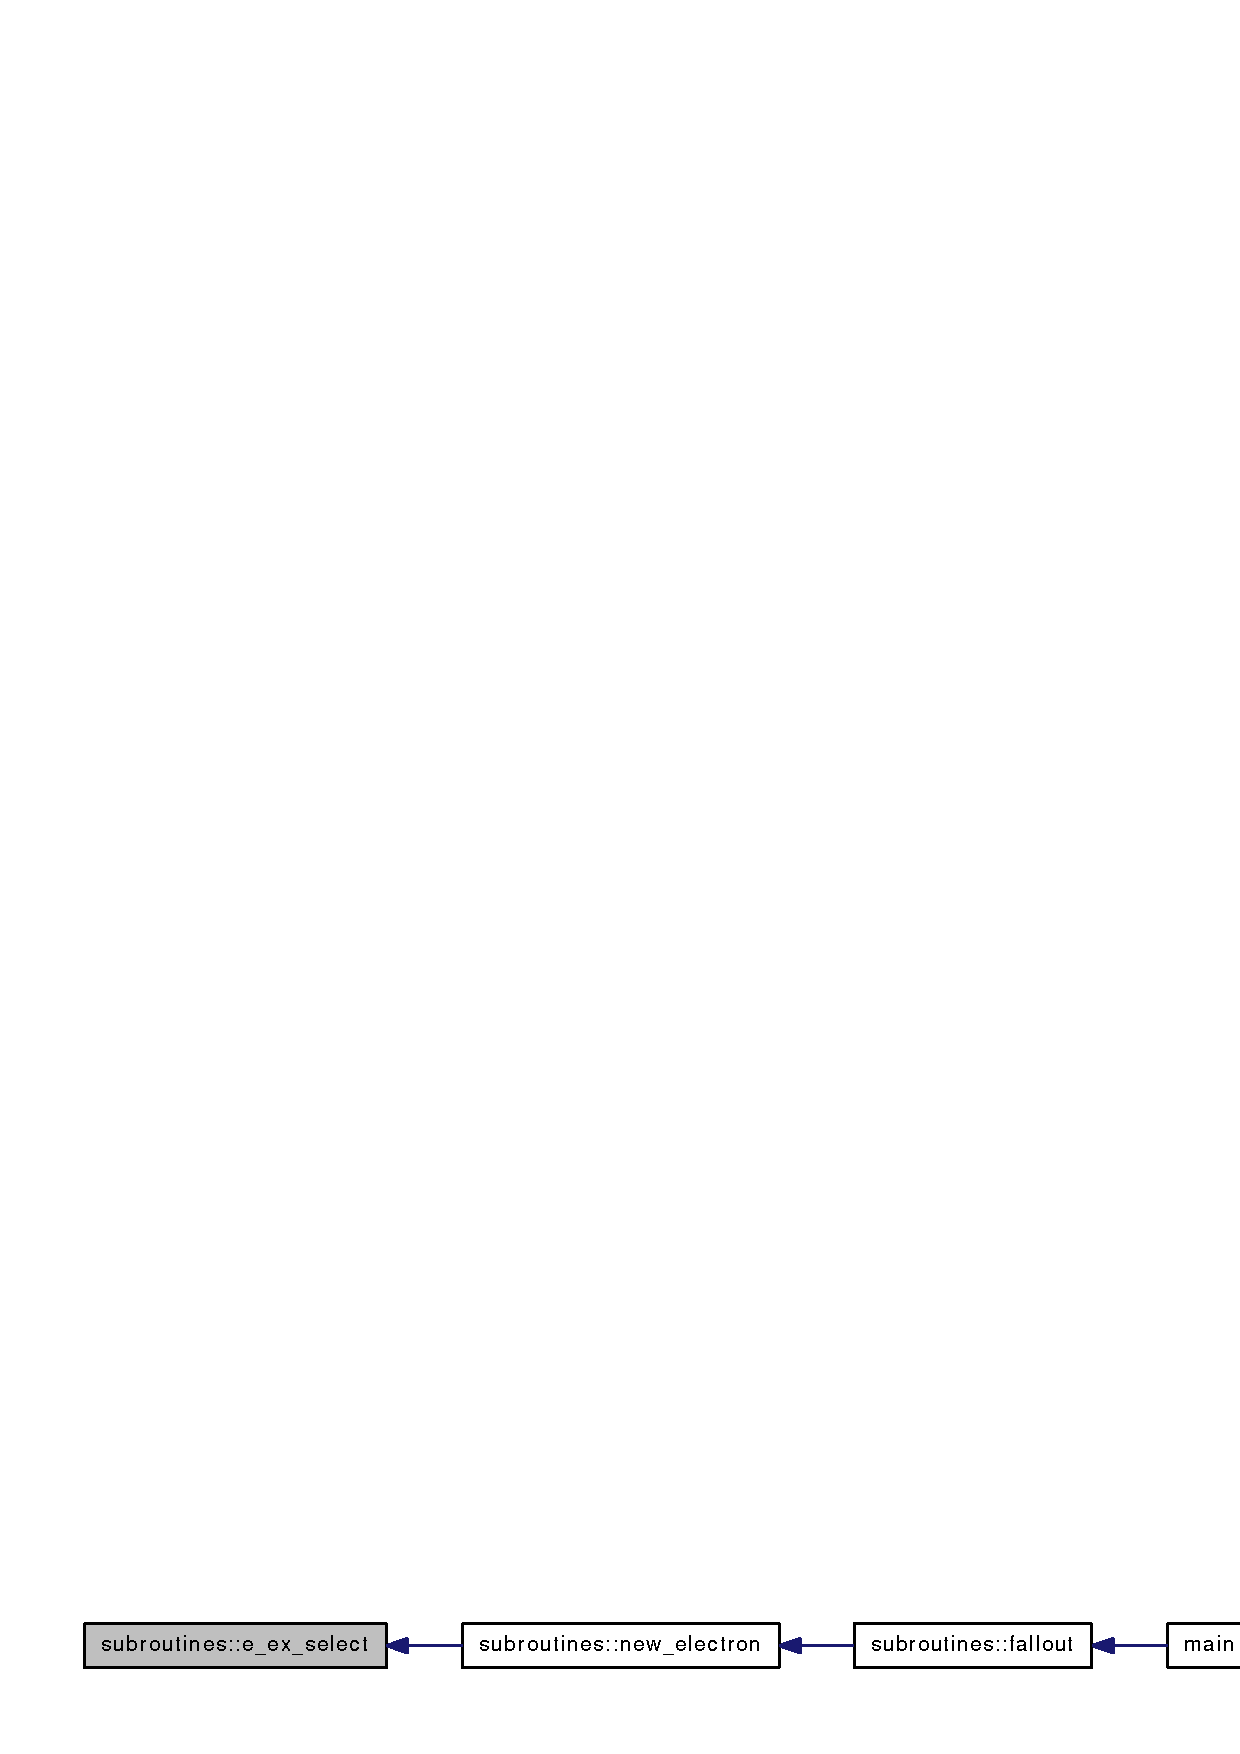
\includegraphics[width=303pt]{namespacesubroutines_a0f09eb60b63730612ddd7801066ce49b_icgraph}
\end{center}
\end{figure}
\hypertarget{namespacesubroutines_acad777e3f27acb4f7e0f7b35035ae54a}{
\index{subroutines@{subroutines}!e\_\-ion\_\-select@{e\_\-ion\_\-select}}
\index{e\_\-ion\_\-select@{e\_\-ion\_\-select}!subroutines@{subroutines}}
\subsubsection[{e\_\-ion\_\-select}]{\setlength{\rightskip}{0pt plus 5cm}subroutine subroutines::e\_\-ion\_\-select (TYPE(se\_\-info) {\em se\_\-box}, \/  DOUBLE PRECISION,intent(out) {\em e\_\-ion}, \/  DOUBLE PRECISION,intent(out) {\em e\_\-se}, \/  INTEGER,intent(out) {\em null}, \/  INTEGER,intent(in) {\em thinghit})}}
\label{namespacesubroutines_acad777e3f27acb4f7e0f7b35035ae54a}


Definition at line 1601 of file subroutines.f90.

References specdata::o3\_\-p\_\-ion, parameters::O3NUM, parameters::O3STARNUM, parameters::ONUM, and parameters::OSTARNUM.

Referenced by new\_\-electron().

Here is the caller graph for this function:\nopagebreak
\begin{figure}[H]
\begin{center}
\leavevmode
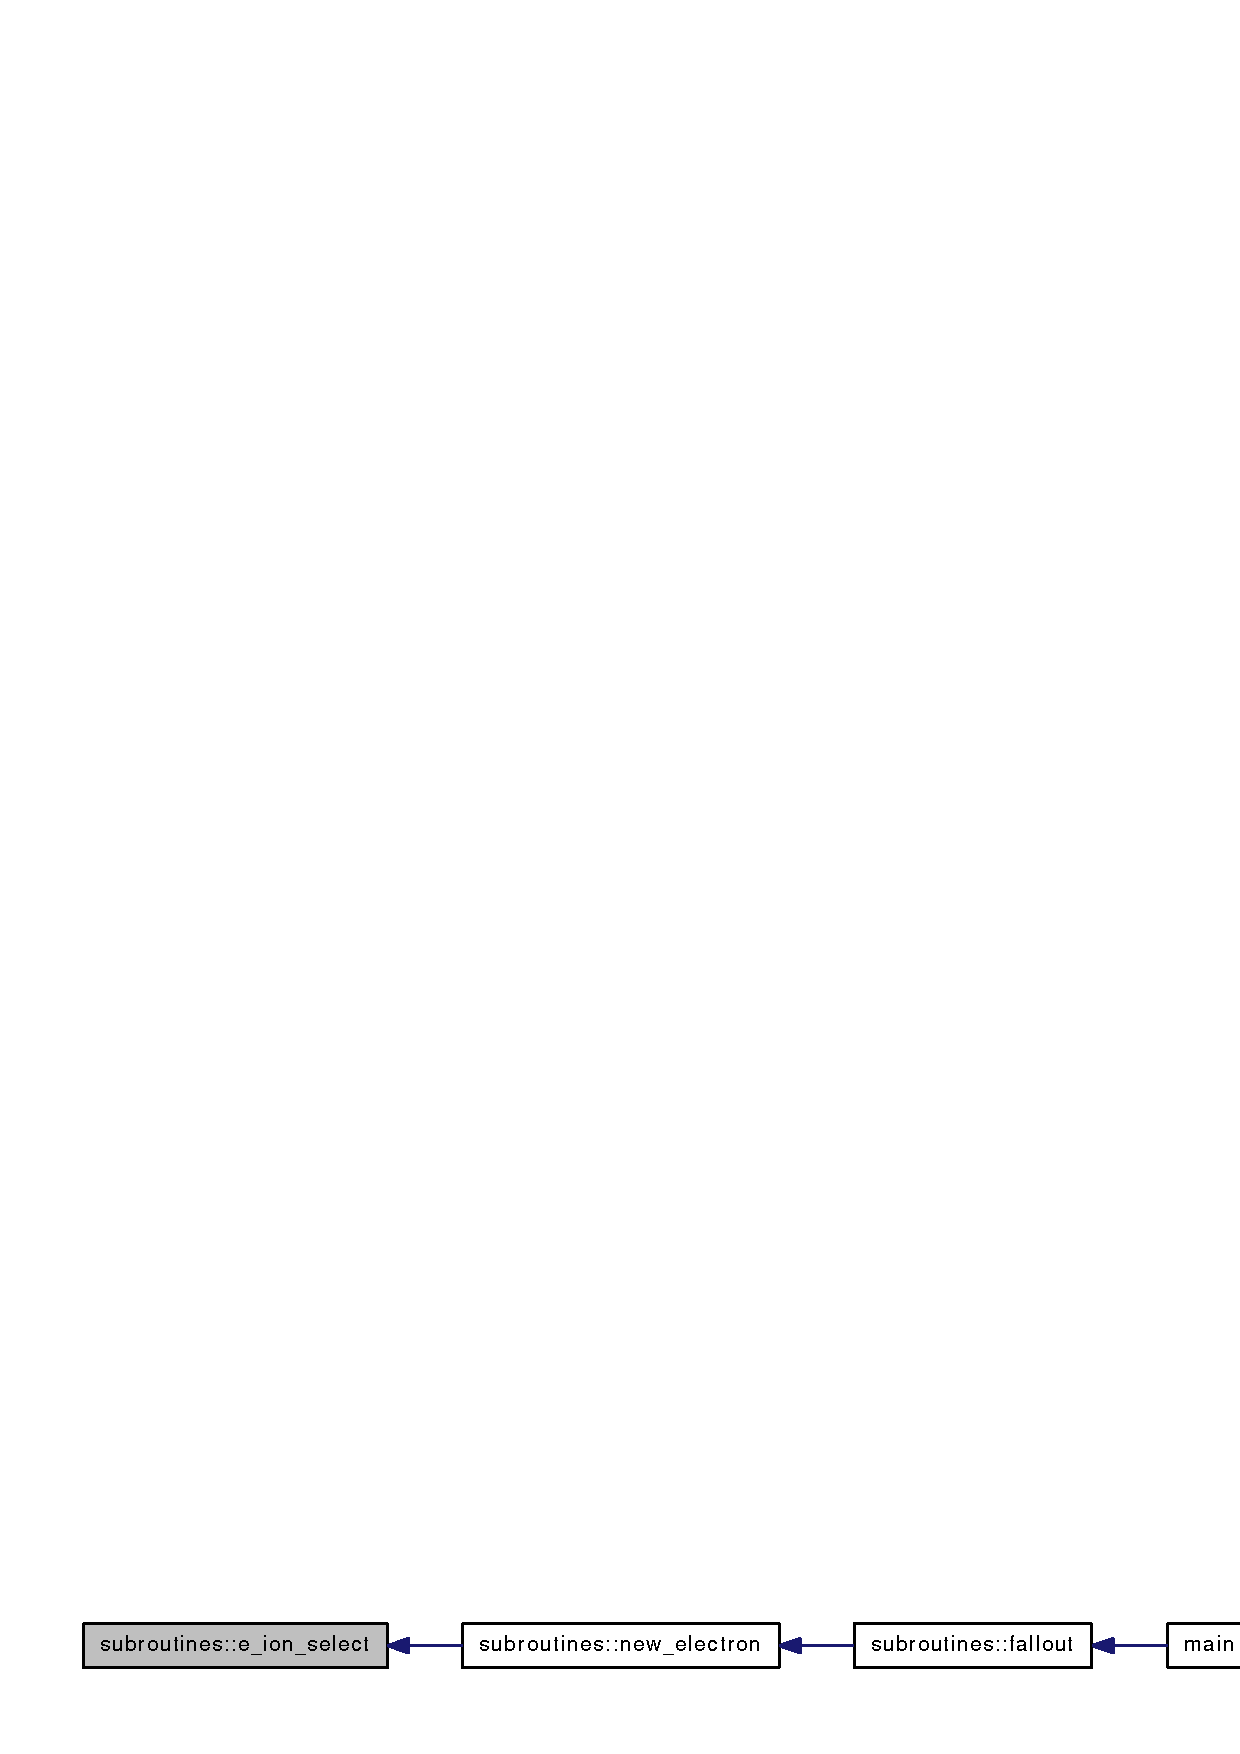
\includegraphics[width=303pt]{namespacesubroutines_acad777e3f27acb4f7e0f7b35035ae54a_icgraph}
\end{center}
\end{figure}
\hypertarget{namespacesubroutines_a10f3c575d44eedaf9b0a95ed9a64e3ab}{
\index{subroutines@{subroutines}!elastic\_\-event@{elastic\_\-event}}
\index{elastic\_\-event@{elastic\_\-event}!subroutines@{subroutines}}
\subsubsection[{elastic\_\-event}]{\setlength{\rightskip}{0pt plus 5cm}subroutine subroutines::elastic\_\-event (DOUBLE PRECISION,pointer {\em energy}, \/  DOUBLE PRECISION,intent(out) {\em e\_\-loss}, \/  DOUBLE PRECISION,intent(out) {\em labtheta})}}
\label{namespacesubroutines_a10f3c575d44eedaf9b0a95ed9a64e3ab}


Definition at line 1853 of file subroutines.f90.

References functiondefs::au(), functiondefs::b\_\-magic(), functiondefs::eps(), functiondefs::lab\_\-theta(), functiondefs::magic(), functiondefs::mass\_\-fac(), parameters::MO2, parameters::MP, parameters::RHO2, functiondefs::t\_\-coll(), parameters::ZO2, and parameters::ZP.

Referenced by fallout().

Here is the call graph for this function:\nopagebreak
\begin{figure}[H]
\begin{center}
\leavevmode
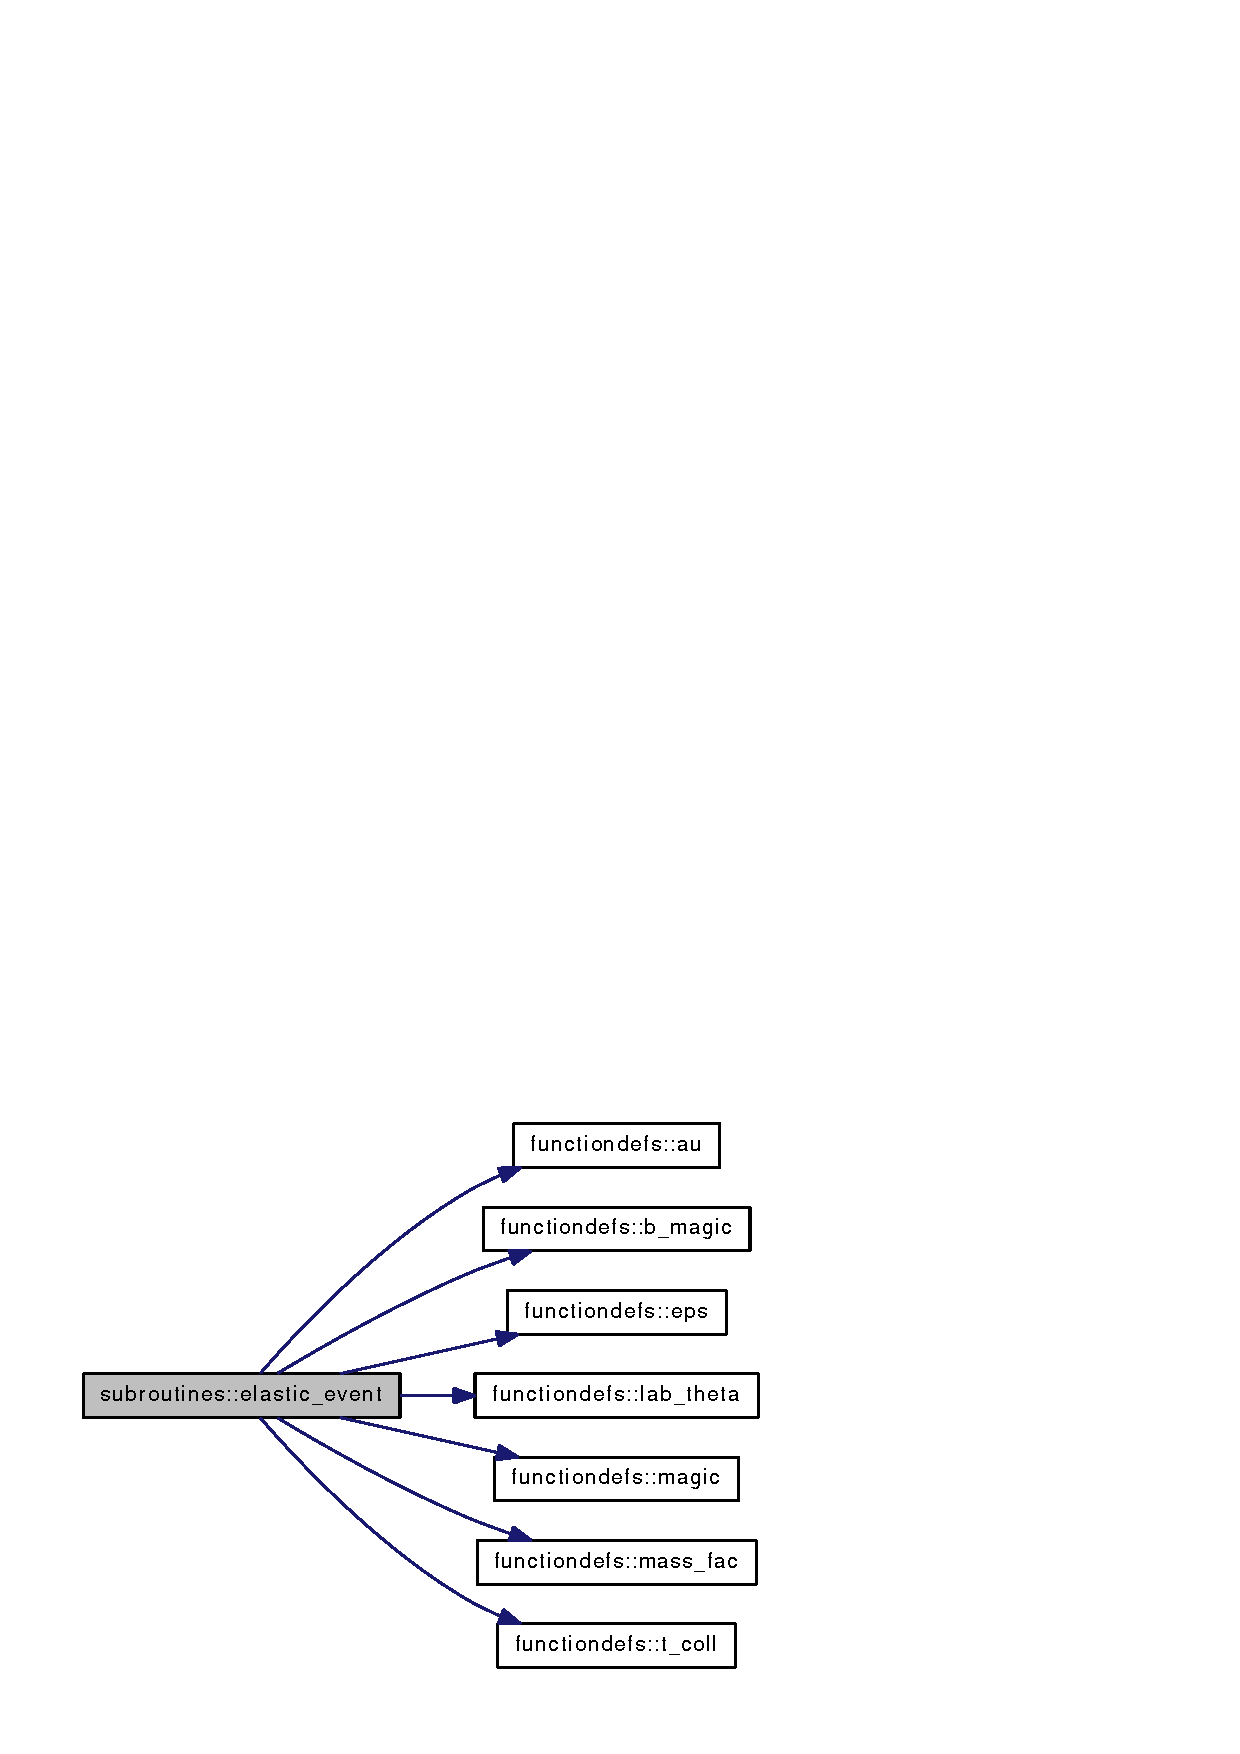
\includegraphics[width=184pt]{namespacesubroutines_a10f3c575d44eedaf9b0a95ed9a64e3ab_cgraph}
\end{center}
\end{figure}


Here is the caller graph for this function:\nopagebreak
\begin{figure}[H]
\begin{center}
\leavevmode
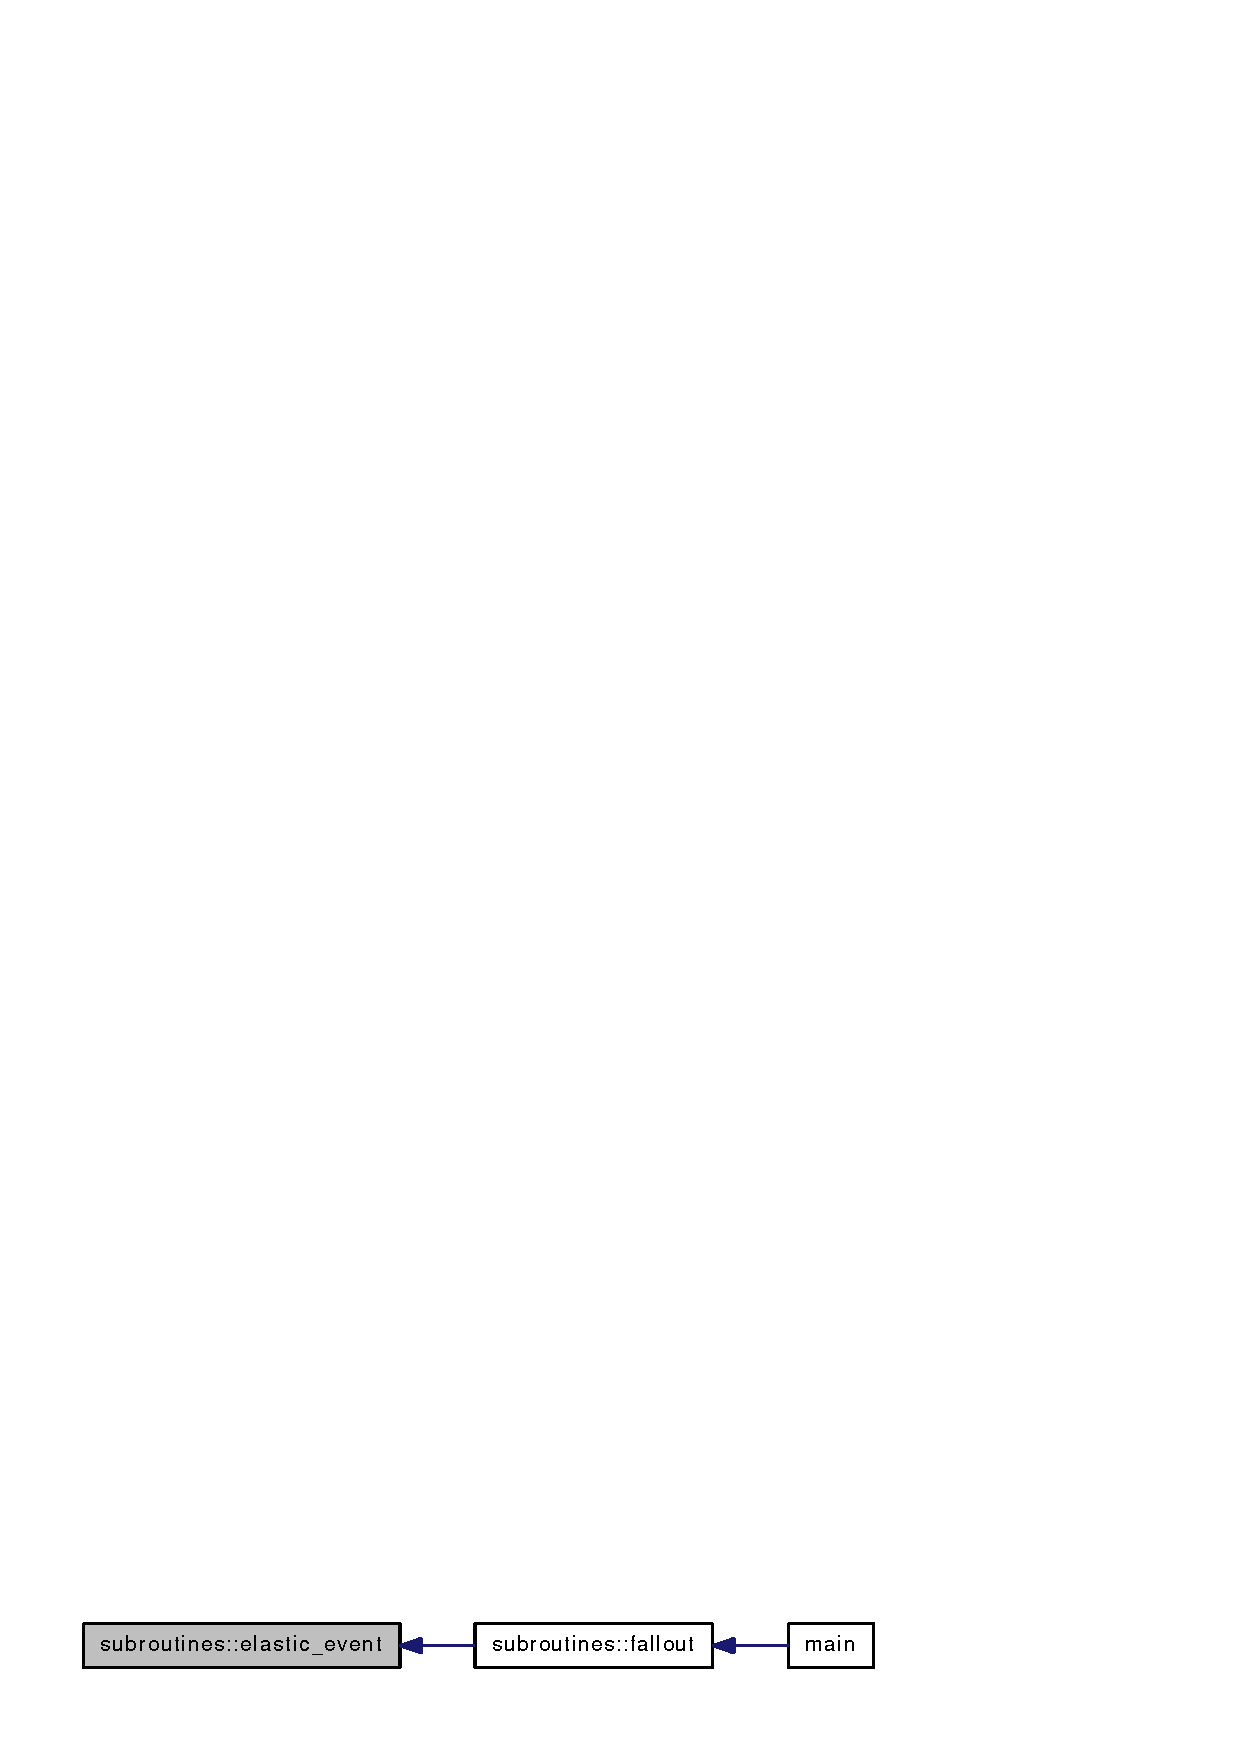
\includegraphics[width=212pt]{namespacesubroutines_a10f3c575d44eedaf9b0a95ed9a64e3ab_icgraph}
\end{center}
\end{figure}
\hypertarget{namespacesubroutines_a27620c6392f4cd49238c295cbe60e179}{
\index{subroutines@{subroutines}!esigma\_\-suite@{esigma\_\-suite}}
\index{esigma\_\-suite@{esigma\_\-suite}!subroutines@{subroutines}}
\subsubsection[{esigma\_\-suite}]{\setlength{\rightskip}{0pt plus 5cm}subroutine subroutines::esigma\_\-suite (TYPE(se\_\-info) {\em se\_\-box})}}
\label{namespacesubroutines_a27620c6392f4cd49238c295cbe60e179}


Definition at line 1248 of file subroutines.f90.

References functiondefs::a\_\-gs(), functiondefs::gamma\_\-gs(), functiondefs::green\_\-mcneal(), functiondefs::green\_\-sawada(), specdata::o2\_\-e\_\-ex\_\-alwd, specdata::o2\_\-e\_\-ex\_\-fbdn, specdata::o3\_\-p\_\-ex, specdata::o3\_\-p\_\-ion, specdata::o\_\-e\_\-ex\_\-alwd, specdata::o\_\-e\_\-ex\_\-fbdn, functiondefs::pjgsigma(), functiondefs::t\_\-0\_\-gs(), functiondefs::t\_\-max\_\-gs(), and parameters::ZO3.

Referenced by new\_\-electron(), and sigma\_\-test().

Here is the call graph for this function:\nopagebreak
\begin{figure}[H]
\begin{center}
\leavevmode
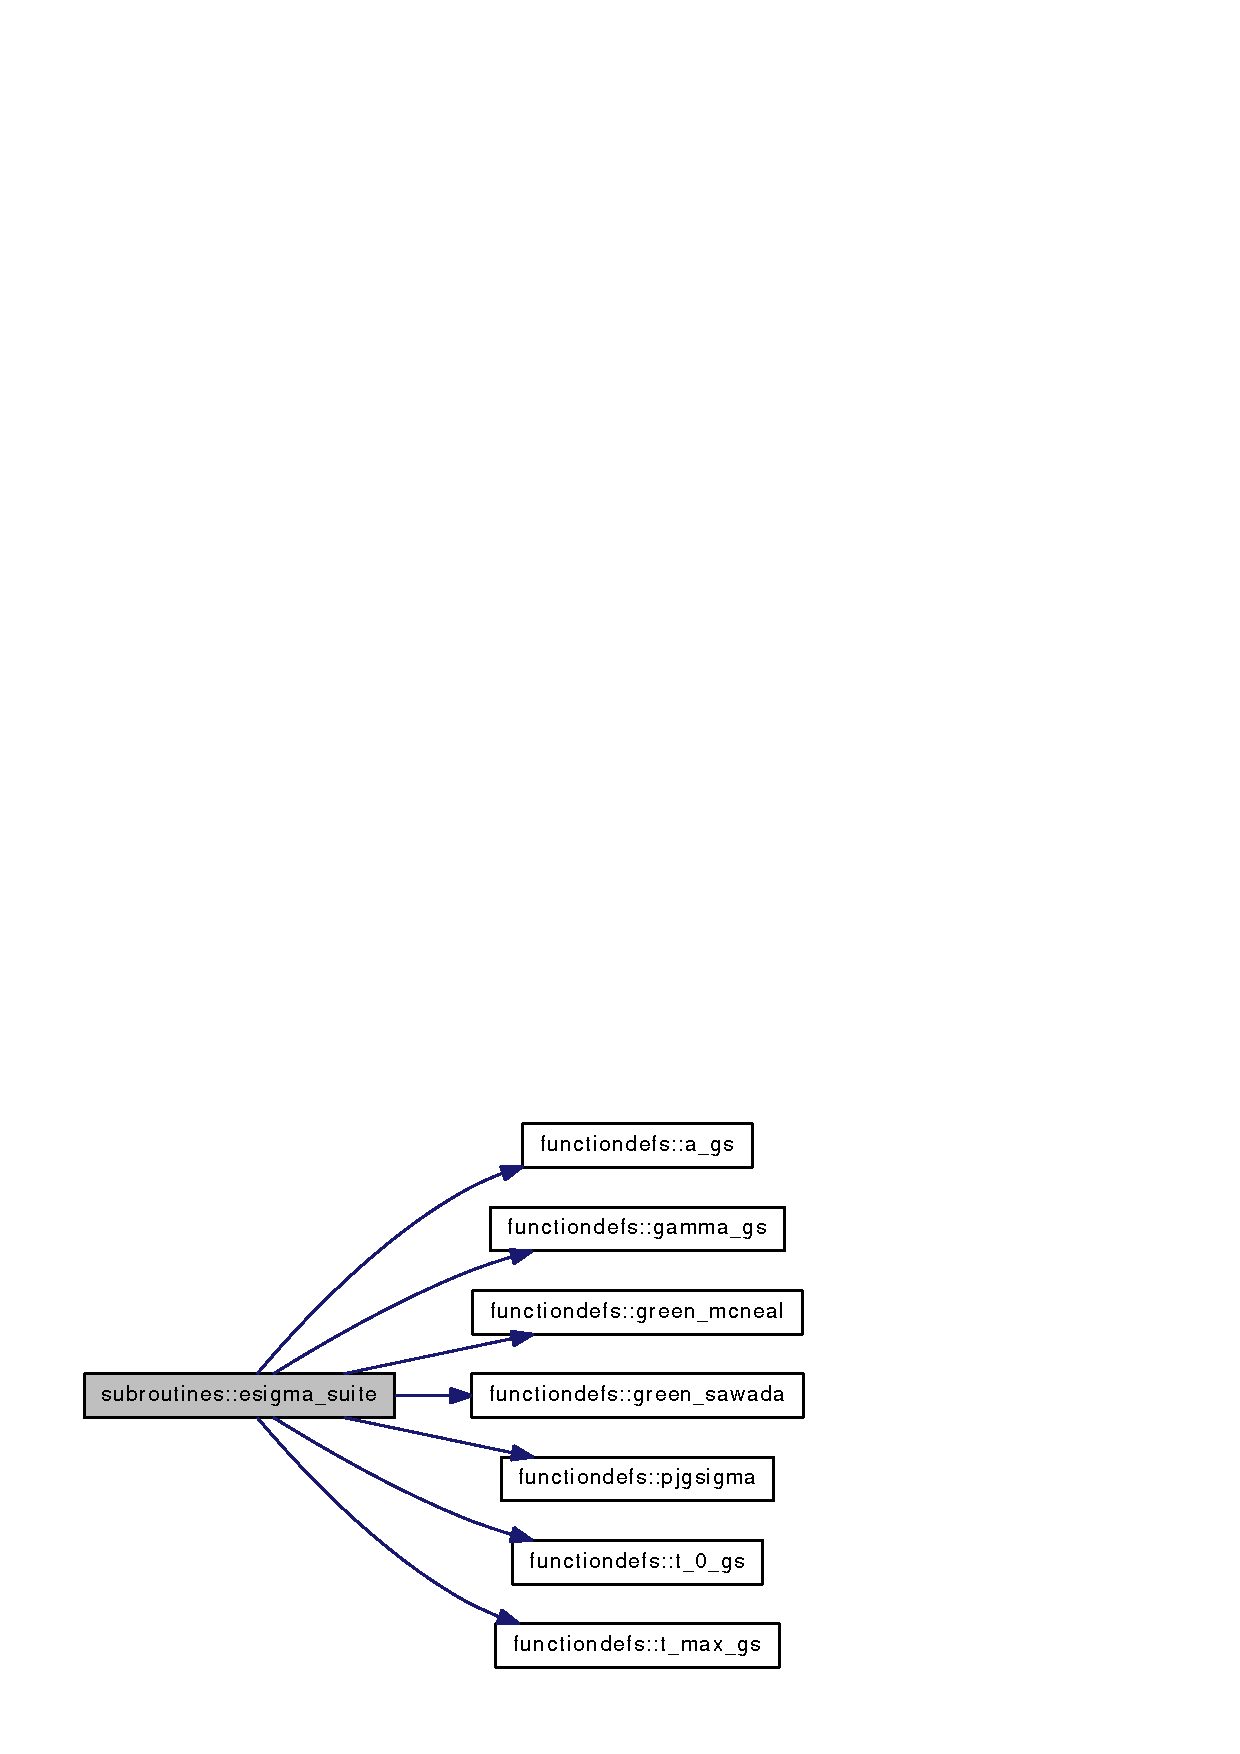
\includegraphics[width=195pt]{namespacesubroutines_a27620c6392f4cd49238c295cbe60e179_cgraph}
\end{center}
\end{figure}


Here is the caller graph for this function:\nopagebreak
\begin{figure}[H]
\begin{center}
\leavevmode
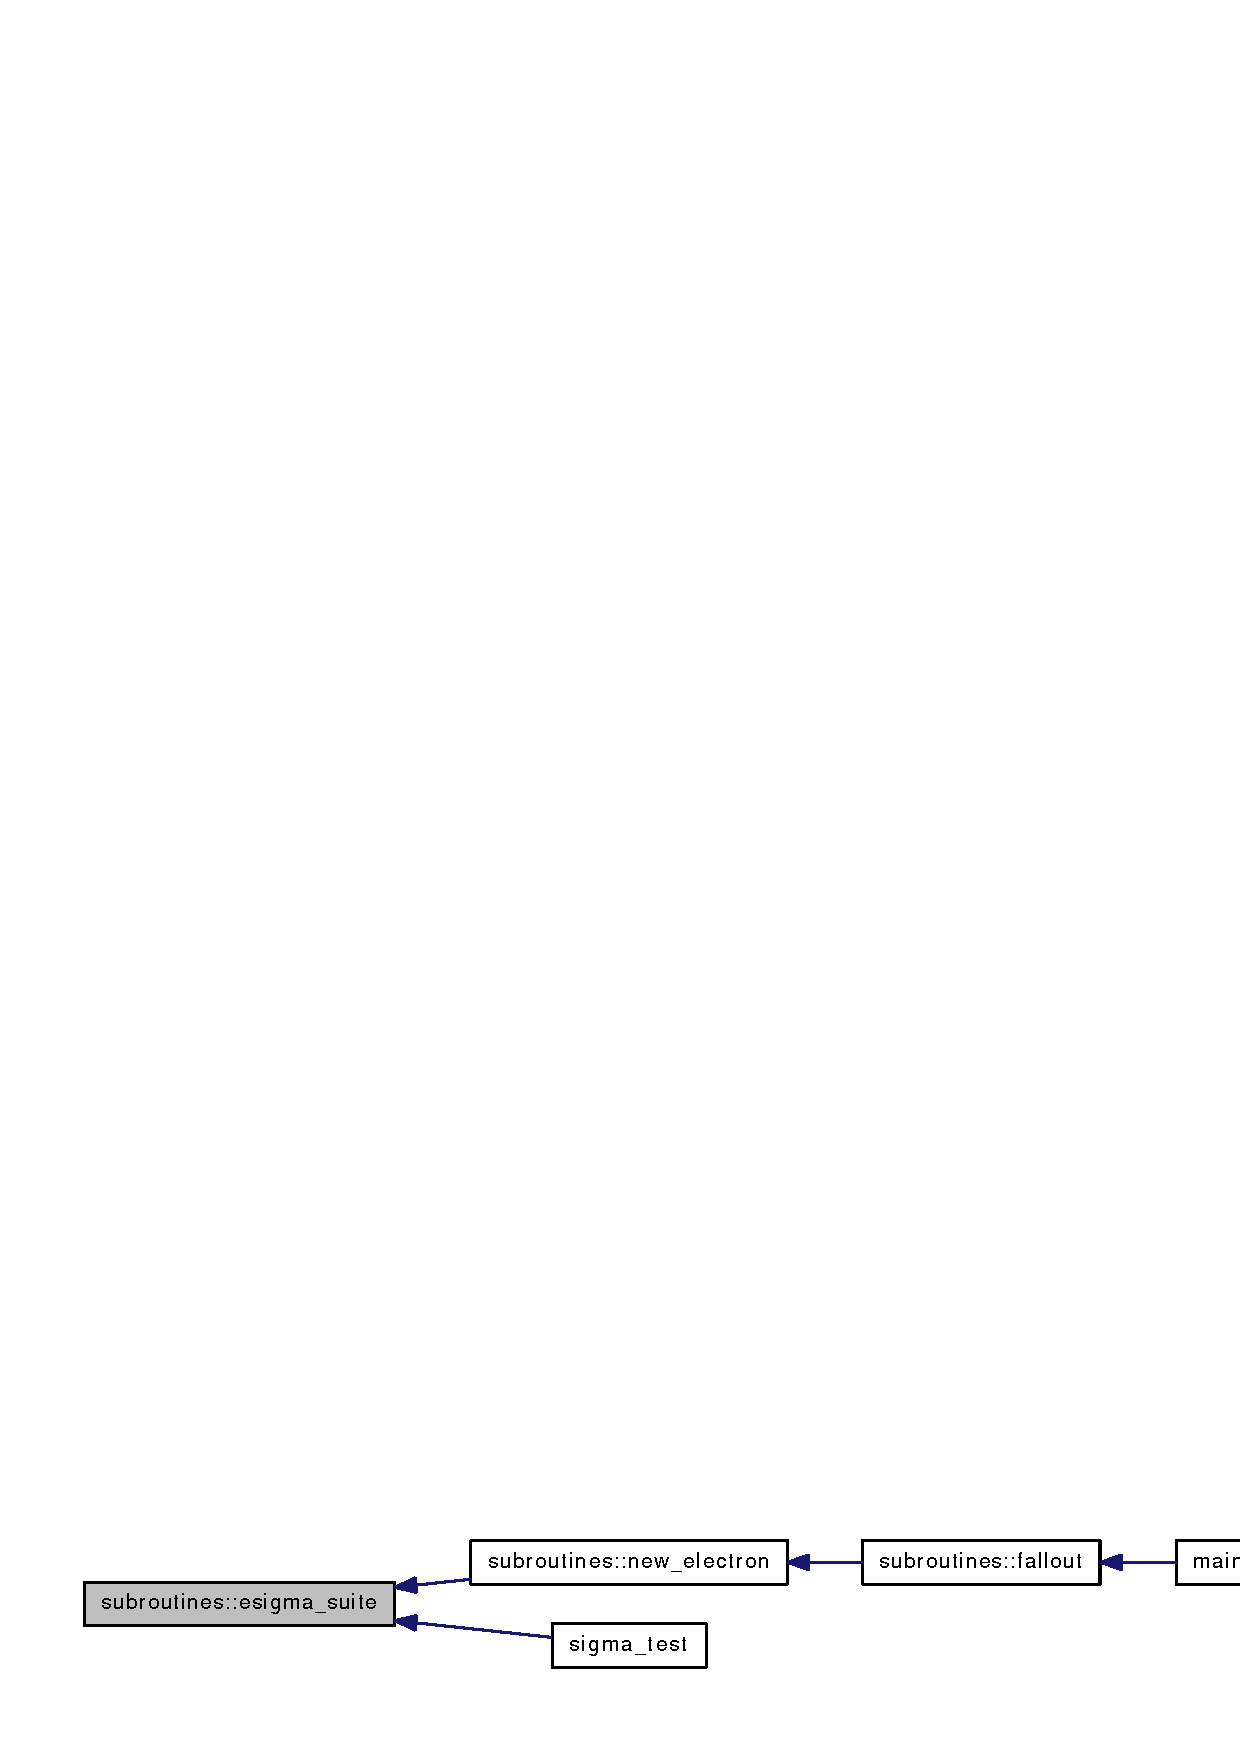
\includegraphics[width=305pt]{namespacesubroutines_a27620c6392f4cd49238c295cbe60e179_icgraph}
\end{center}
\end{figure}
\hypertarget{namespacesubroutines_a7a31d5c9fbda24651c932b0466618567}{
\index{subroutines@{subroutines}!fallout@{fallout}}
\index{fallout@{fallout}!subroutines@{subroutines}}
\subsubsection[{fallout}]{\setlength{\rightskip}{0pt plus 5cm}subroutine subroutines::fallout (TYPE(node),pointer {\em root}, \/  TYPE(node),pointer {\em temp}, \/  TYPE(node),pointer {\em prevNode}, \/  TYPE(node),pointer {\em nextNode})}}
\label{namespacesubroutines_a7a31d5c9fbda24651c932b0466618567}


Definition at line 217 of file subroutines.f90.

References parameters::BI\_\-CALLS, parameters::CRPNUM, parameters::DEBUG, parameters::DIMENS, parameters::EINIT, elastic\_\-event(), parameters::ELECNUM, parameters::EXCNUM, parameters::IONLIST, parameters::MATRIX, new\_\-electron(), new\_\-reaction(), specdata::o2\_\-p\_\-ex, specdata::o2\_\-p\_\-ion, specdata::o3\_\-p\_\-ex, specdata::o3\_\-p\_\-ion, specdata::o\_\-p\_\-ex, specdata::o\_\-p\_\-ion, p\_\-ex\_\-select(), p\_\-ion\_\-select(), parameters::PMODEL, parameters::PROTON\_\-COLL, parameters::PROTON\_\-ELOSS, psigma\_\-suite(), se\_\-info\_\-garbage(), se\_\-info\_\-init(), parameters::SECELEC, parameters::STEPFAC, parameters::THICK, parameters::TRACKMAX, parameters::TRACKMIN, parameters::TRACKPLOT, parameters::TRACKPLOT\_\-LUN, and trackwrite().

Referenced by main().

Here is the call graph for this function:\nopagebreak
\begin{figure}[H]
\begin{center}
\leavevmode
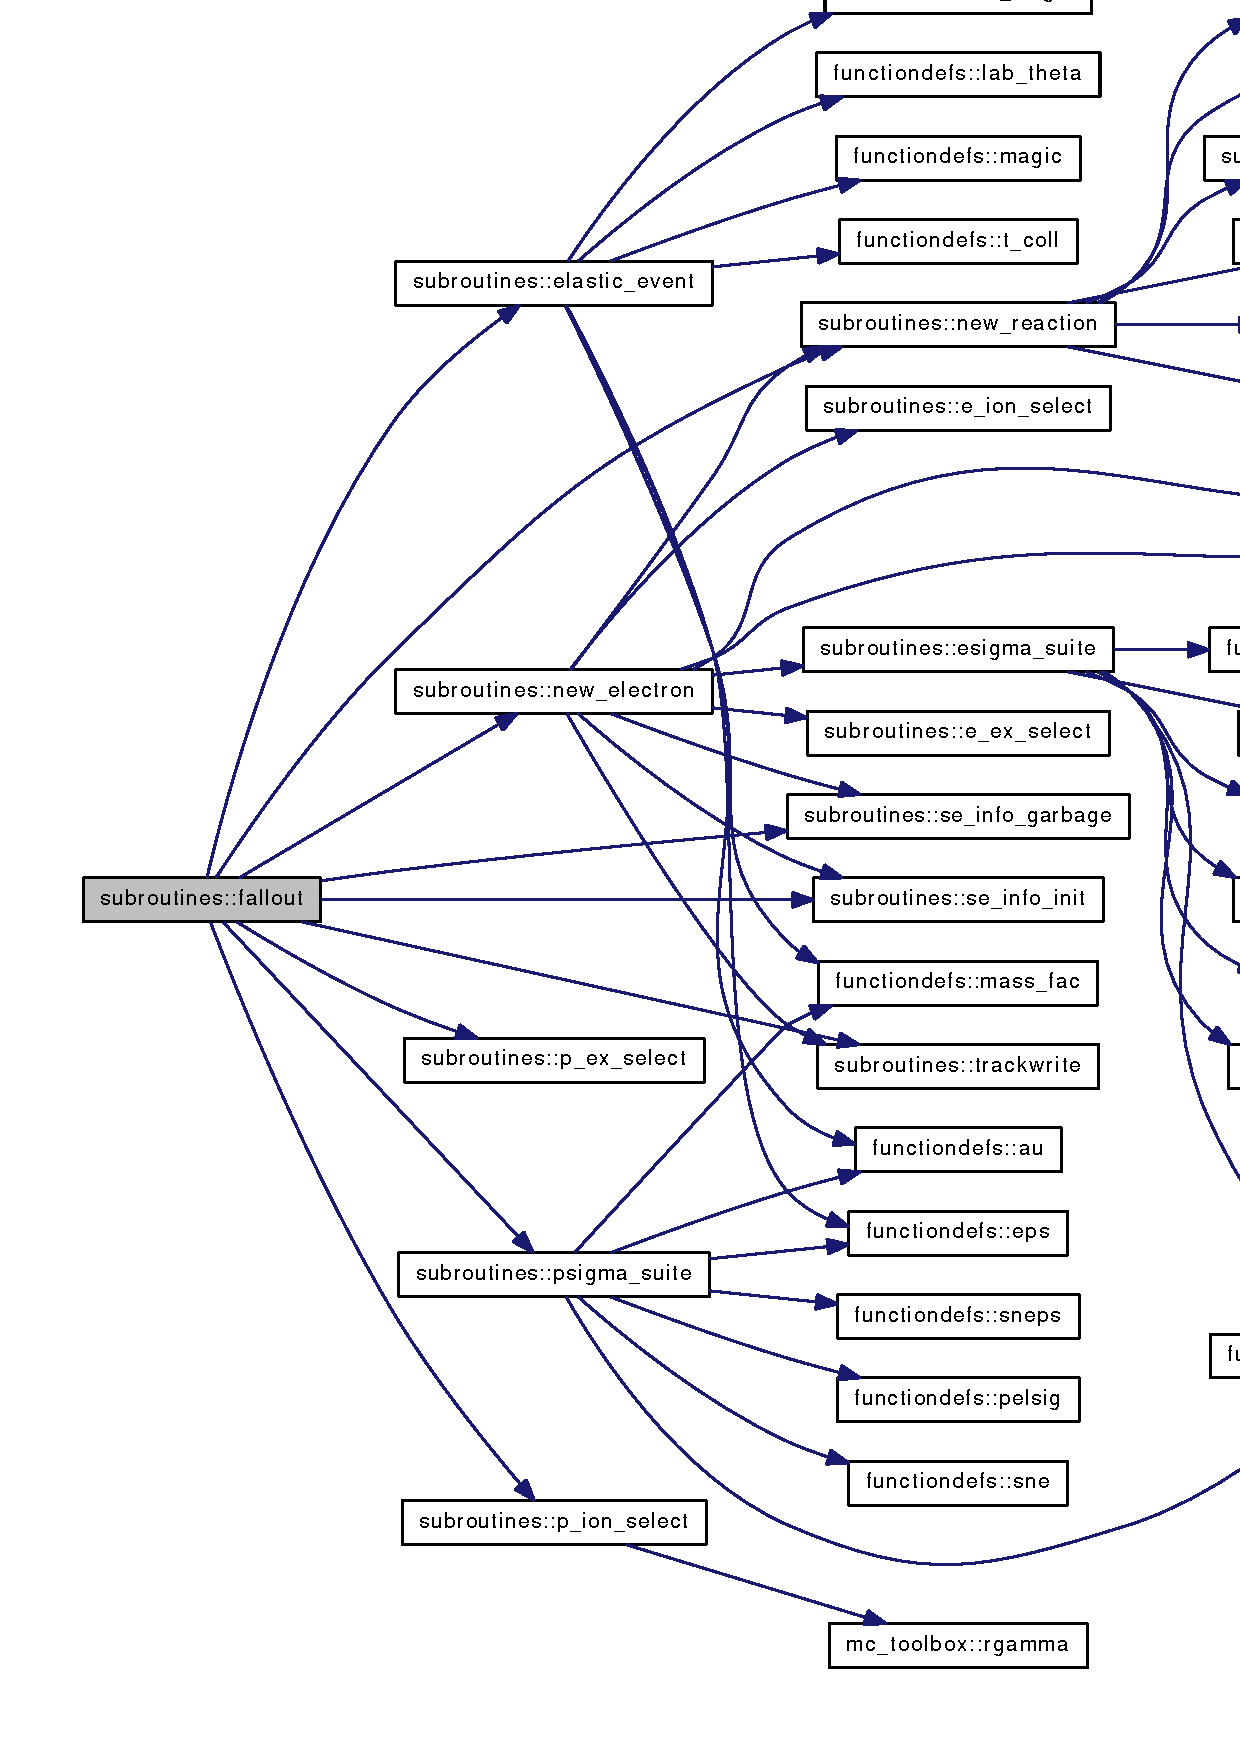
\includegraphics[width=420pt]{namespacesubroutines_a7a31d5c9fbda24651c932b0466618567_cgraph}
\end{center}
\end{figure}


Here is the caller graph for this function:\nopagebreak
\begin{figure}[H]
\begin{center}
\leavevmode
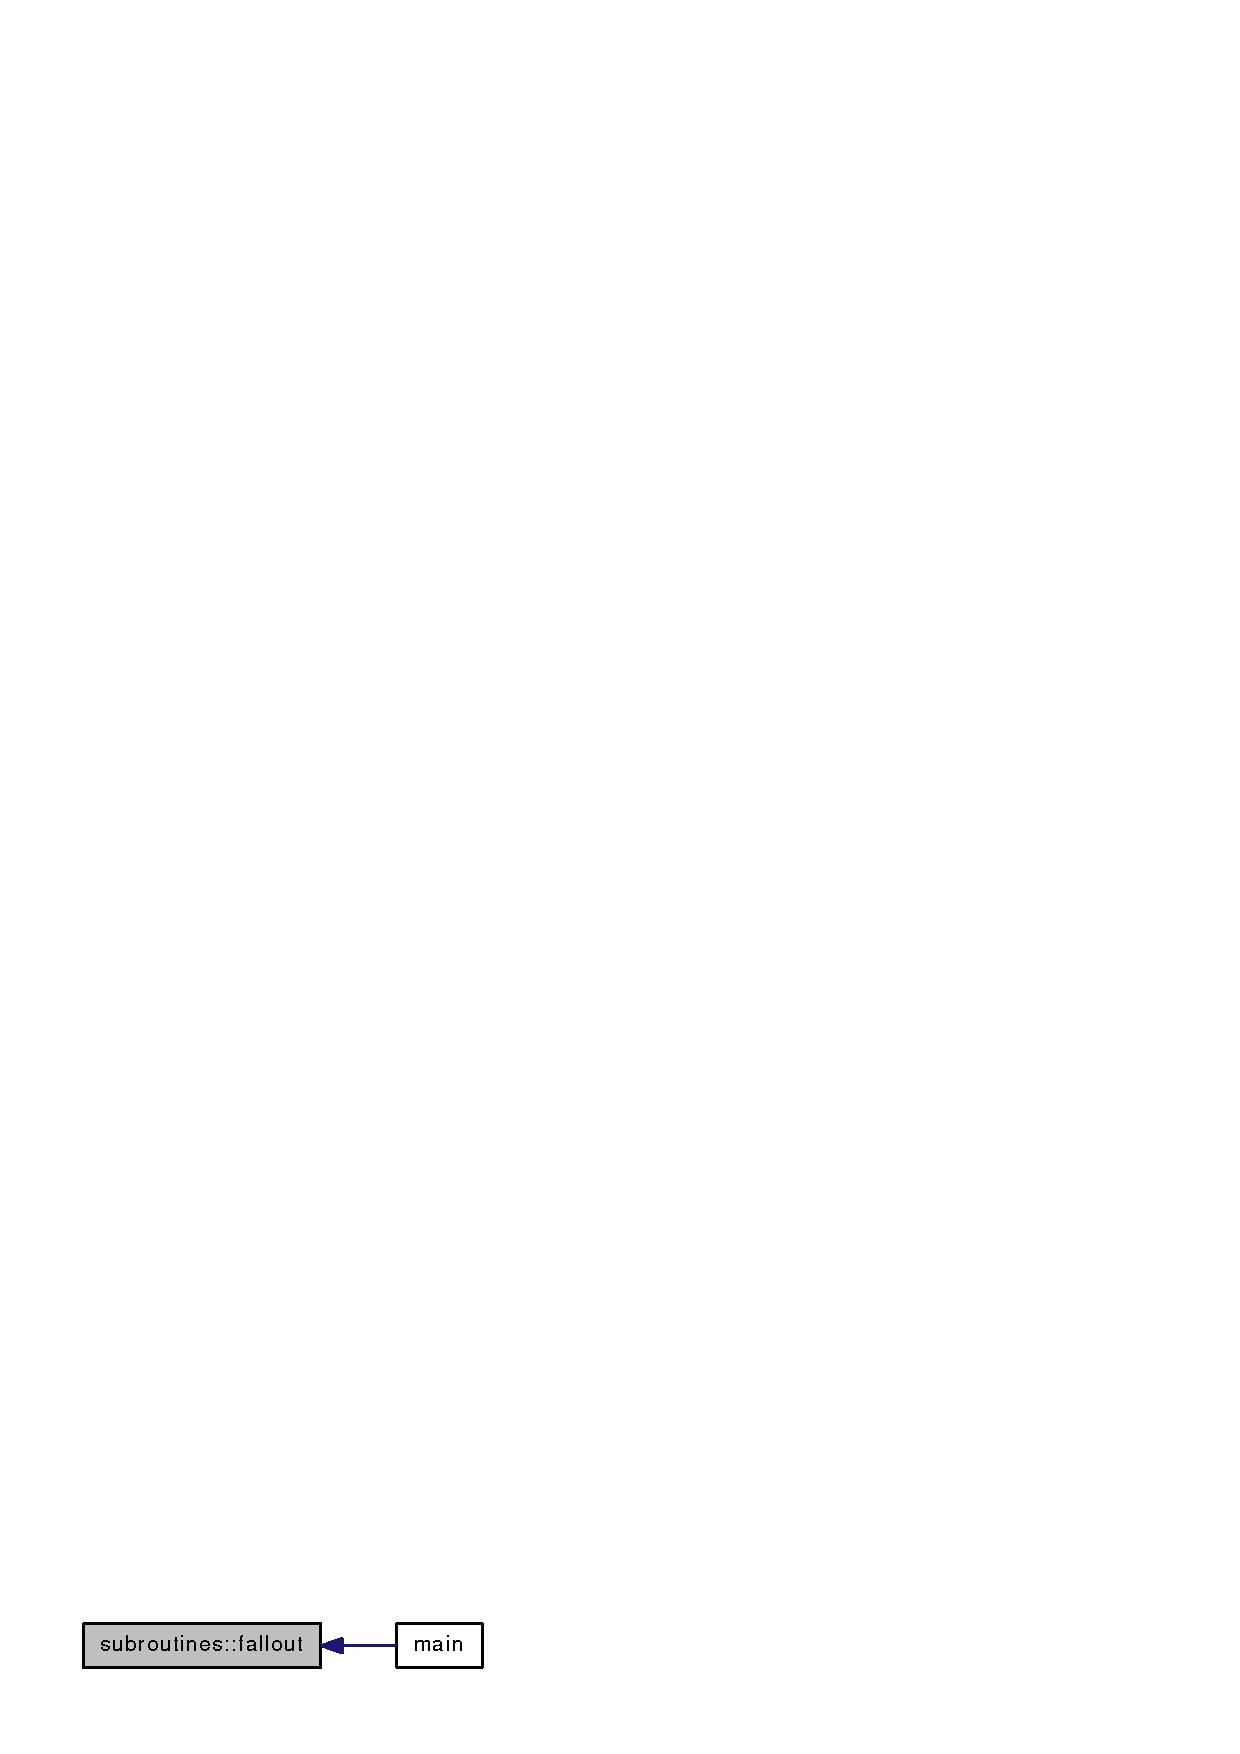
\includegraphics[width=118pt]{namespacesubroutines_a7a31d5c9fbda24651c932b0466618567_icgraph}
\end{center}
\end{figure}
\hypertarget{namespacesubroutines_af4c69699bd3e0e4aa05607a7e94044dc}{
\index{subroutines@{subroutines}!find\_\-empty\_\-site@{find\_\-empty\_\-site}}
\index{find\_\-empty\_\-site@{find\_\-empty\_\-site}!subroutines@{subroutines}}
\subsubsection[{find\_\-empty\_\-site}]{\setlength{\rightskip}{0pt plus 5cm}subroutine subroutines::find\_\-empty\_\-site (INTEGER,dimension(3),intent(in) {\em in\_\-coords}, \/  INTEGER,dimension(3),intent(out) {\em out\_\-coords}, \/  INTEGER {\em null})}}
\label{namespacesubroutines_af4c69699bd3e0e4aa05607a7e94044dc}


Definition at line 547 of file subroutines.f90.

References parameters::DEBUG, parameters::DIMENS, parameters::FIND\_\-EMPTY\_\-COUNT, parameters::FINDMAX, hopping(), parameters::MATRIX, and transport().

Referenced by new\_\-reaction().

Here is the call graph for this function:\nopagebreak
\begin{figure}[H]
\begin{center}
\leavevmode
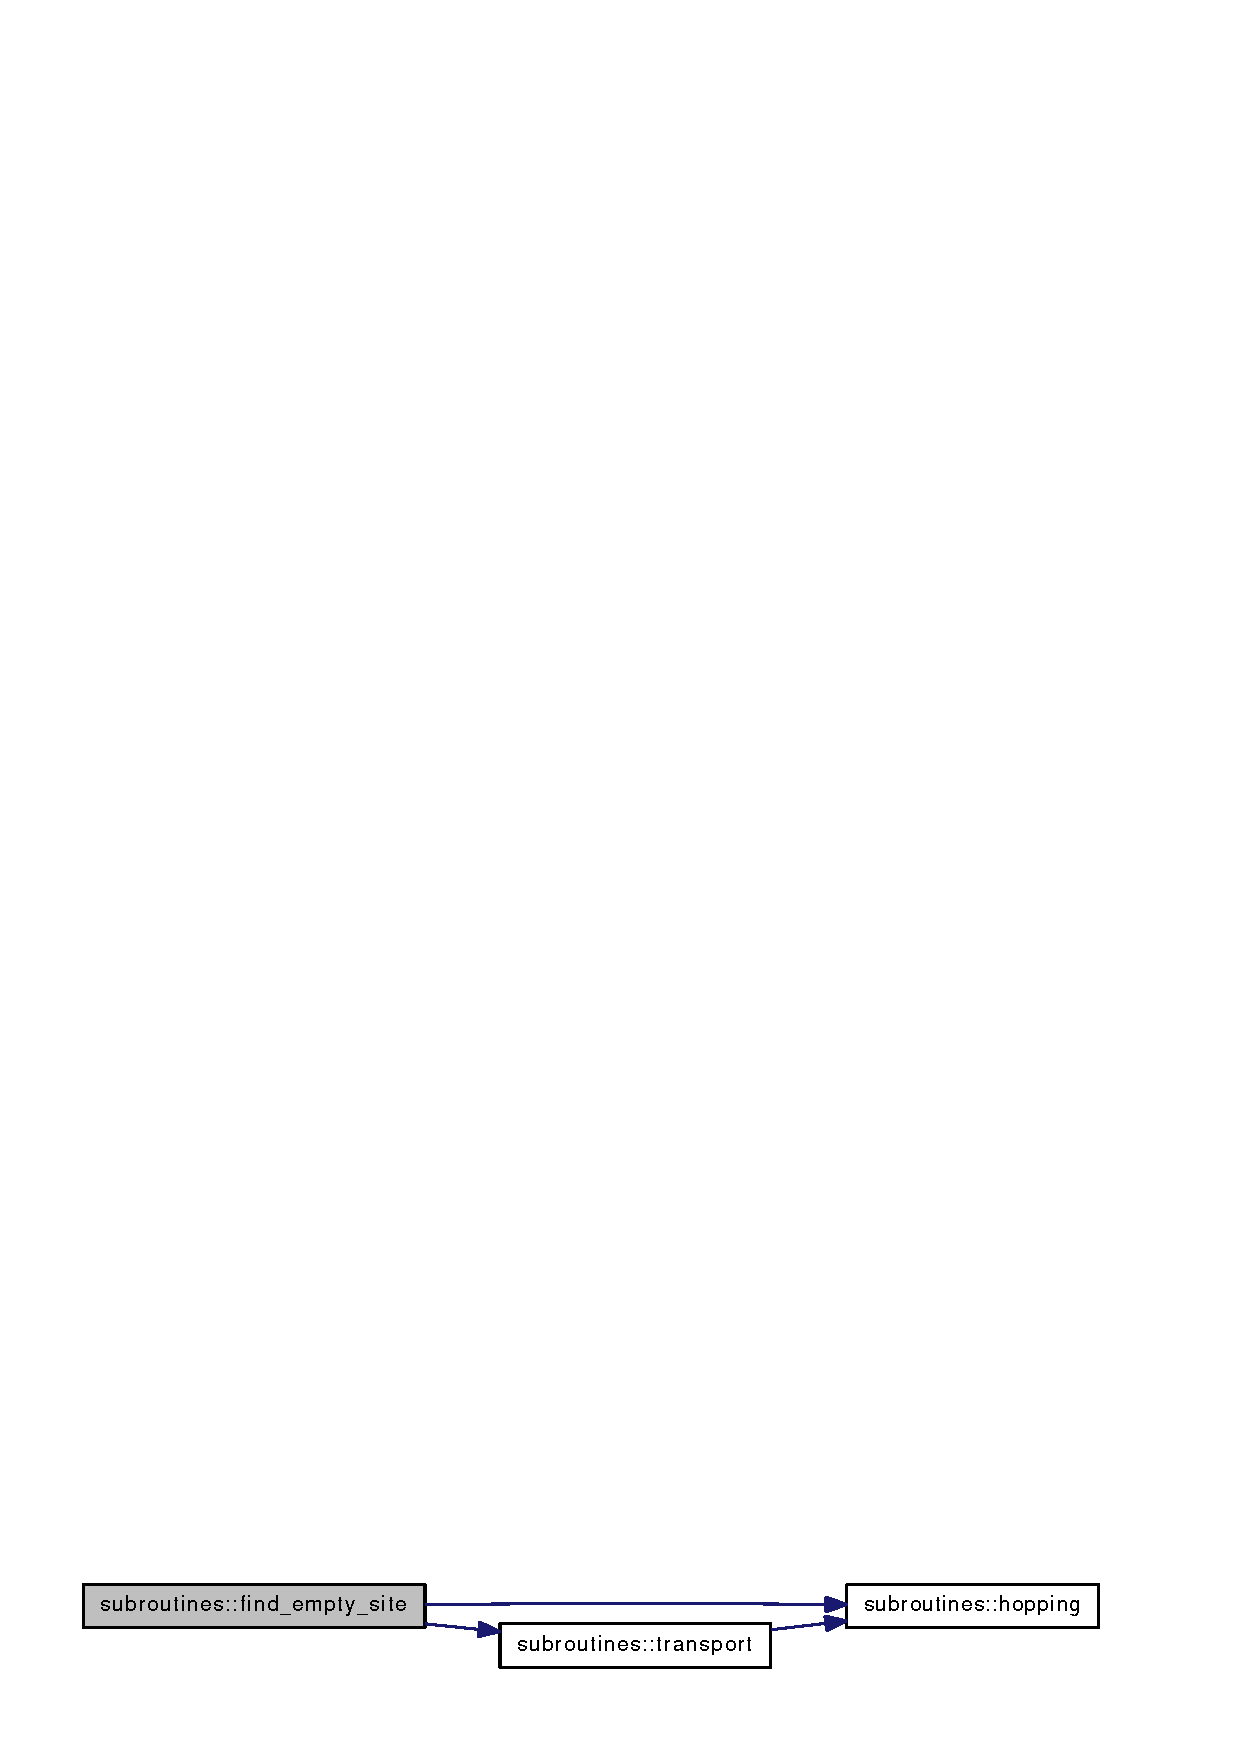
\includegraphics[width=266pt]{namespacesubroutines_af4c69699bd3e0e4aa05607a7e94044dc_cgraph}
\end{center}
\end{figure}


Here is the caller graph for this function:\nopagebreak
\begin{figure}[H]
\begin{center}
\leavevmode
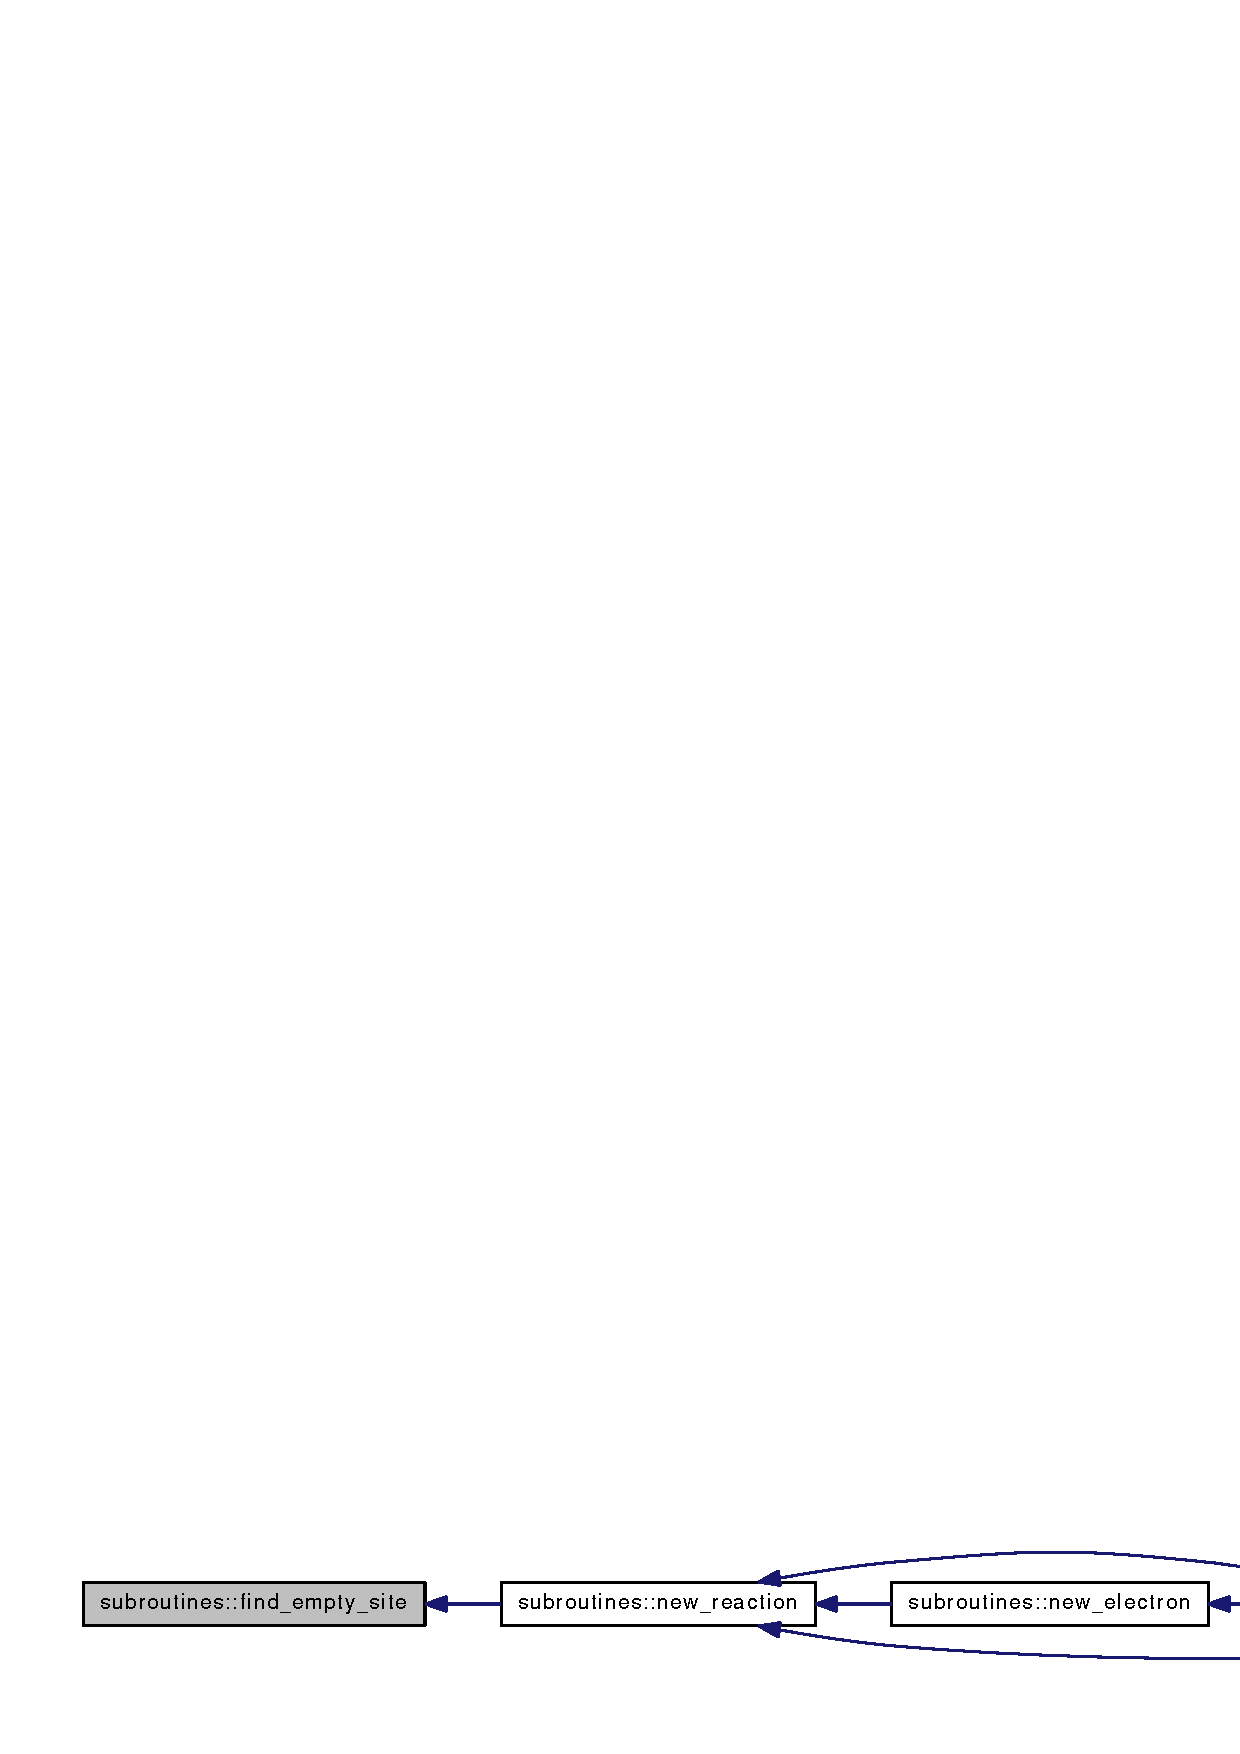
\includegraphics[width=406pt]{namespacesubroutines_af4c69699bd3e0e4aa05607a7e94044dc_icgraph}
\end{center}
\end{figure}
\hypertarget{namespacesubroutines_ad97e0b9db9cfe6329f9f8fdb886077e7}{
\index{subroutines@{subroutines}!hopping@{hopping}}
\index{hopping@{hopping}!subroutines@{subroutines}}
\subsubsection[{hopping}]{\setlength{\rightskip}{0pt plus 5cm}subroutine subroutines::hopping (INTEGER,intent(in) {\em i\_\-in}, \/  INTEGER,intent(in) {\em j\_\-in}, \/  INTEGER,intent(in) {\em k\_\-in}, \/  INTEGER,intent(out) {\em i\_\-out}, \/  INTEGER,intent(out) {\em j\_\-out}, \/  INTEGER,intent(out) {\em k\_\-out}, \/  INTEGER,intent(in) {\em prob})}}
\label{namespacesubroutines_ad97e0b9db9cfe6329f9f8fdb886077e7}


Definition at line 113 of file subroutines.f90.

References parameters::DIMENS.

Referenced by find\_\-empty\_\-site(), main(), new\_\-electron(), transport(), and wait\_\-calc().

Here is the caller graph for this function:\nopagebreak
\begin{figure}[H]
\begin{center}
\leavevmode
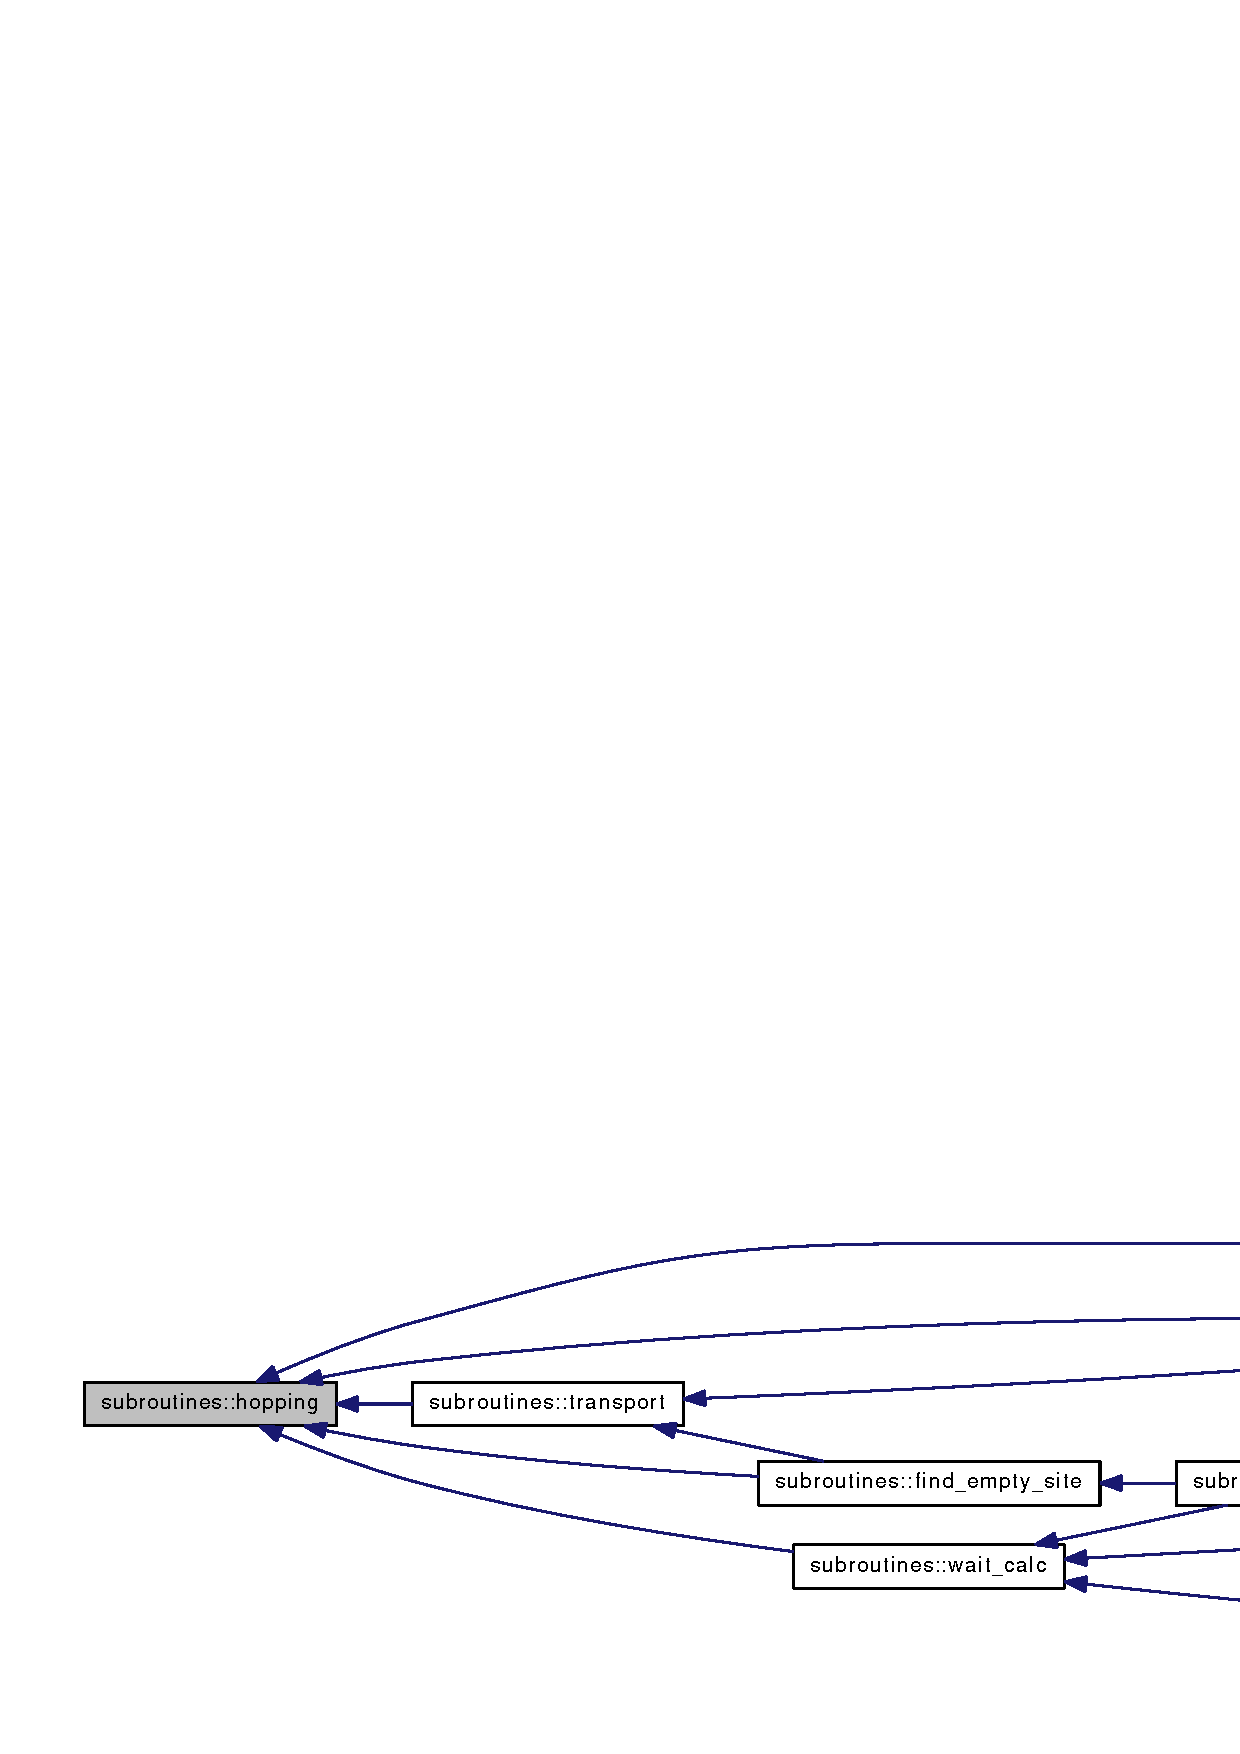
\includegraphics[width=420pt]{namespacesubroutines_ad97e0b9db9cfe6329f9f8fdb886077e7_icgraph}
\end{center}
\end{figure}
\hypertarget{namespacesubroutines_a4d9b1fbbdcfc2b420201a7ca71c4e782}{
\index{subroutines@{subroutines}!init\_\-node@{init\_\-node}}
\index{init\_\-node@{init\_\-node}!subroutines@{subroutines}}
\subsubsection[{init\_\-node}]{\setlength{\rightskip}{0pt plus 5cm}subroutine subroutines::init\_\-node (TYPE(node),pointer {\em root}, \/  TYPE(node),pointer {\em temp\_\-node}, \/  INTEGER {\em x}, \/  INTEGER {\em y}, \/  INTEGER {\em z})}}
\label{namespacesubroutines_a4d9b1fbbdcfc2b420201a7ca71c4e782}


Definition at line 1977 of file subroutines.f90.

References bsimple::add\_\-node(), parameters::DEBUG, and wait\_\-calc().

Referenced by main().

Here is the call graph for this function:\nopagebreak
\begin{figure}[H]
\begin{center}
\leavevmode
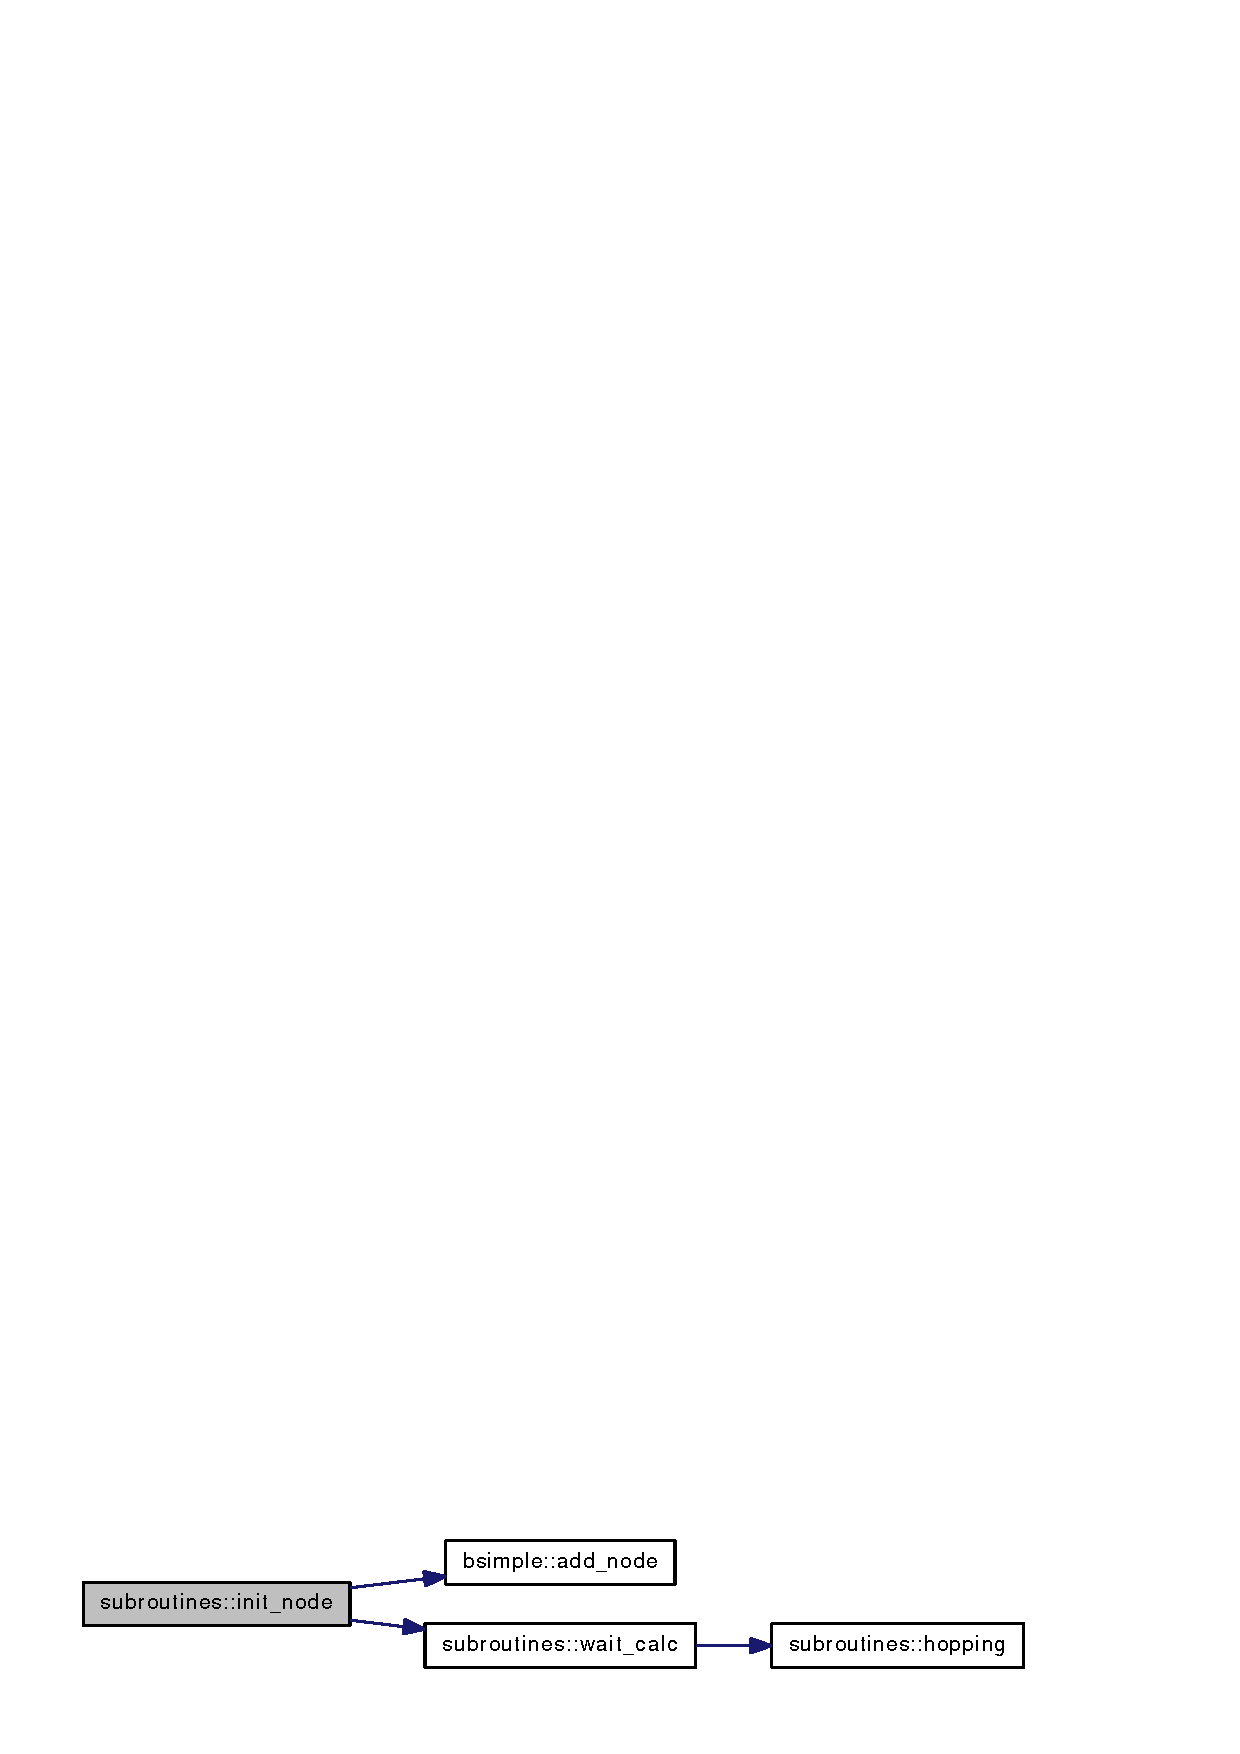
\includegraphics[width=248pt]{namespacesubroutines_a4d9b1fbbdcfc2b420201a7ca71c4e782_cgraph}
\end{center}
\end{figure}


Here is the caller graph for this function:\nopagebreak
\begin{figure}[H]
\begin{center}
\leavevmode
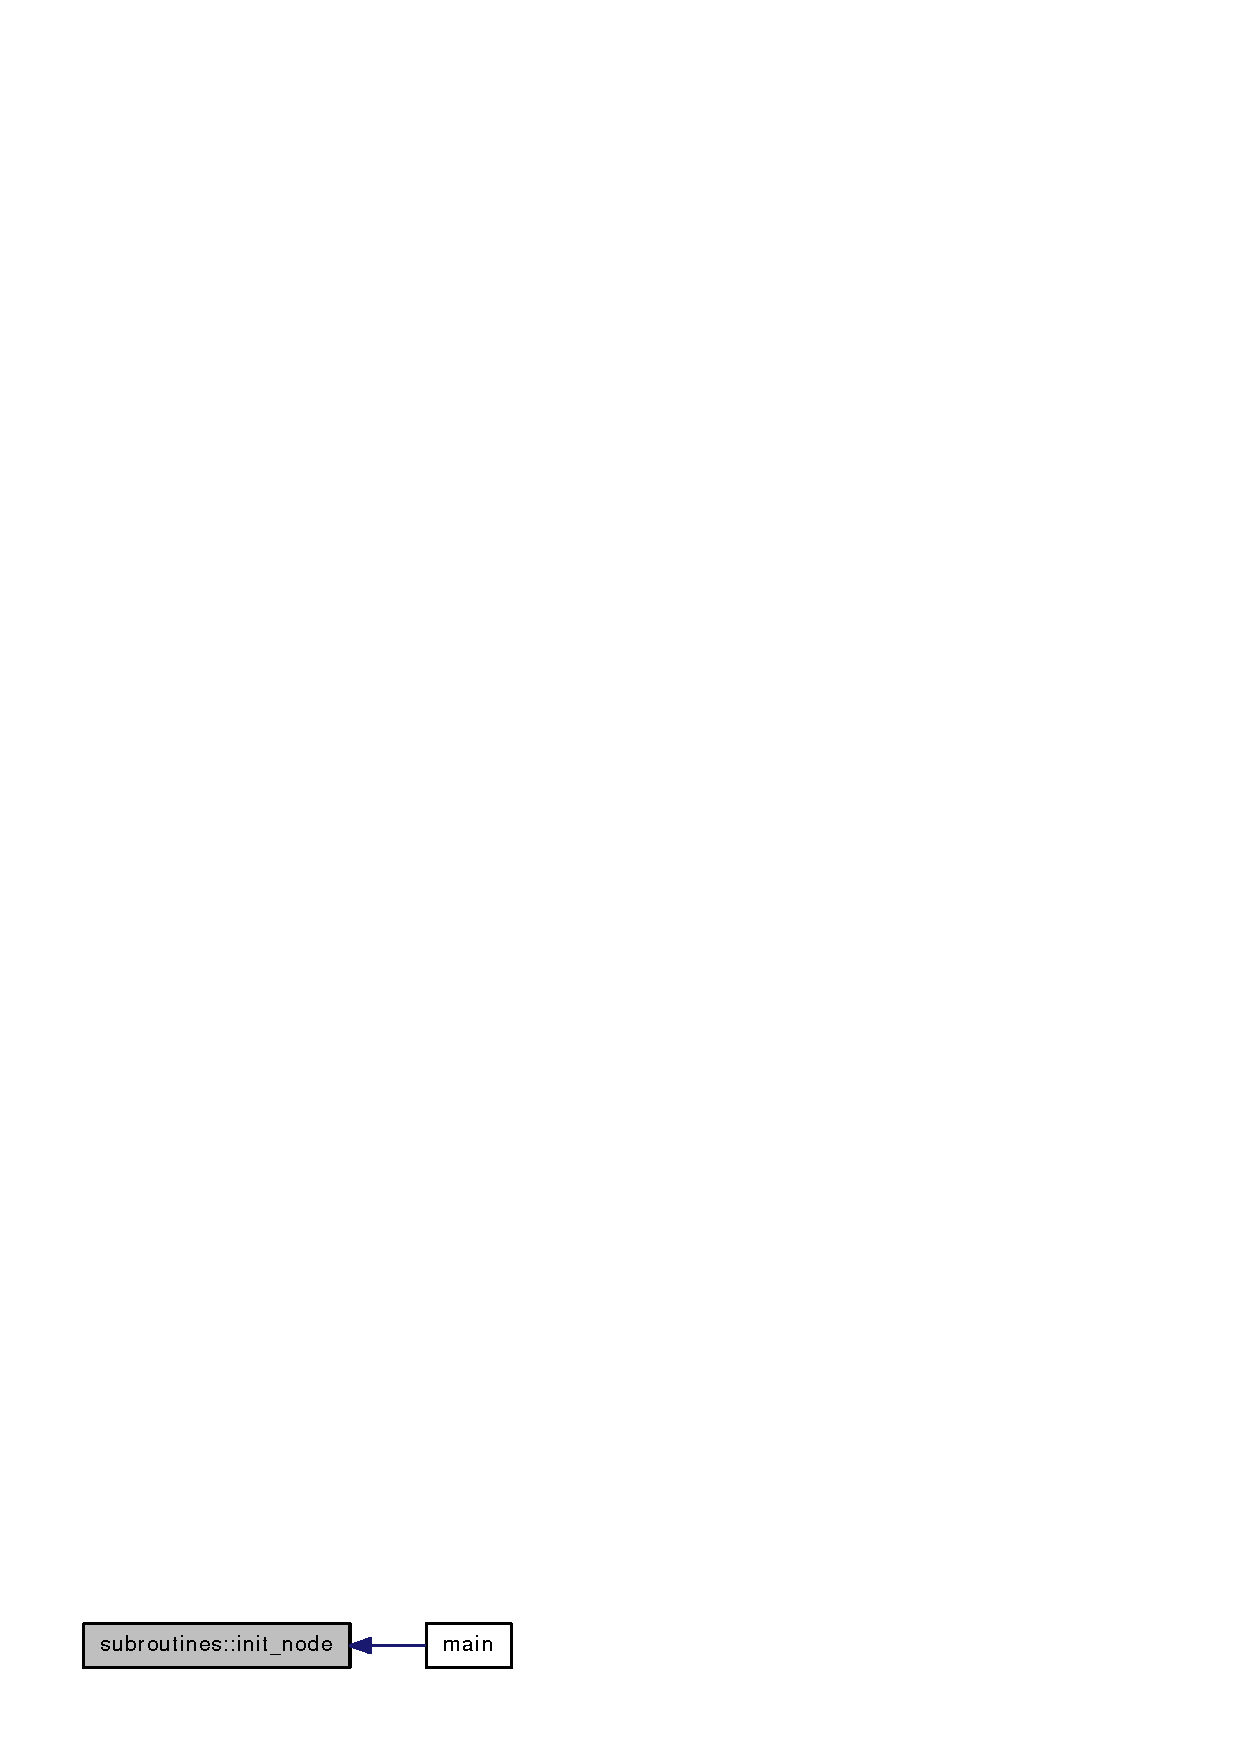
\includegraphics[width=125pt]{namespacesubroutines_a4d9b1fbbdcfc2b420201a7ca71c4e782_icgraph}
\end{center}
\end{figure}
\hypertarget{namespacesubroutines_a27505ee5071c93bb5f1e570995a1ac42}{
\index{subroutines@{subroutines}!lookup@{lookup}}
\index{lookup@{lookup}!subroutines@{subroutines}}
\subsubsection[{lookup}]{\setlength{\rightskip}{0pt plus 5cm}subroutine subroutines::lookup (CHARACTER(len=10) {\em name}, \/  TYPE(species) {\em node}, \/  INTEGER {\em id}, \/  INTEGER {\em atoms}, \/  INTEGER {\em charge})}}
\label{namespacesubroutines_a27505ee5071c93bb5f1e570995a1ac42}


Definition at line 13 of file subroutines.f90.

Referenced by readinput::buildnetwork(), and qbert().

Here is the caller graph for this function:\nopagebreak
\begin{figure}[H]
\begin{center}
\leavevmode
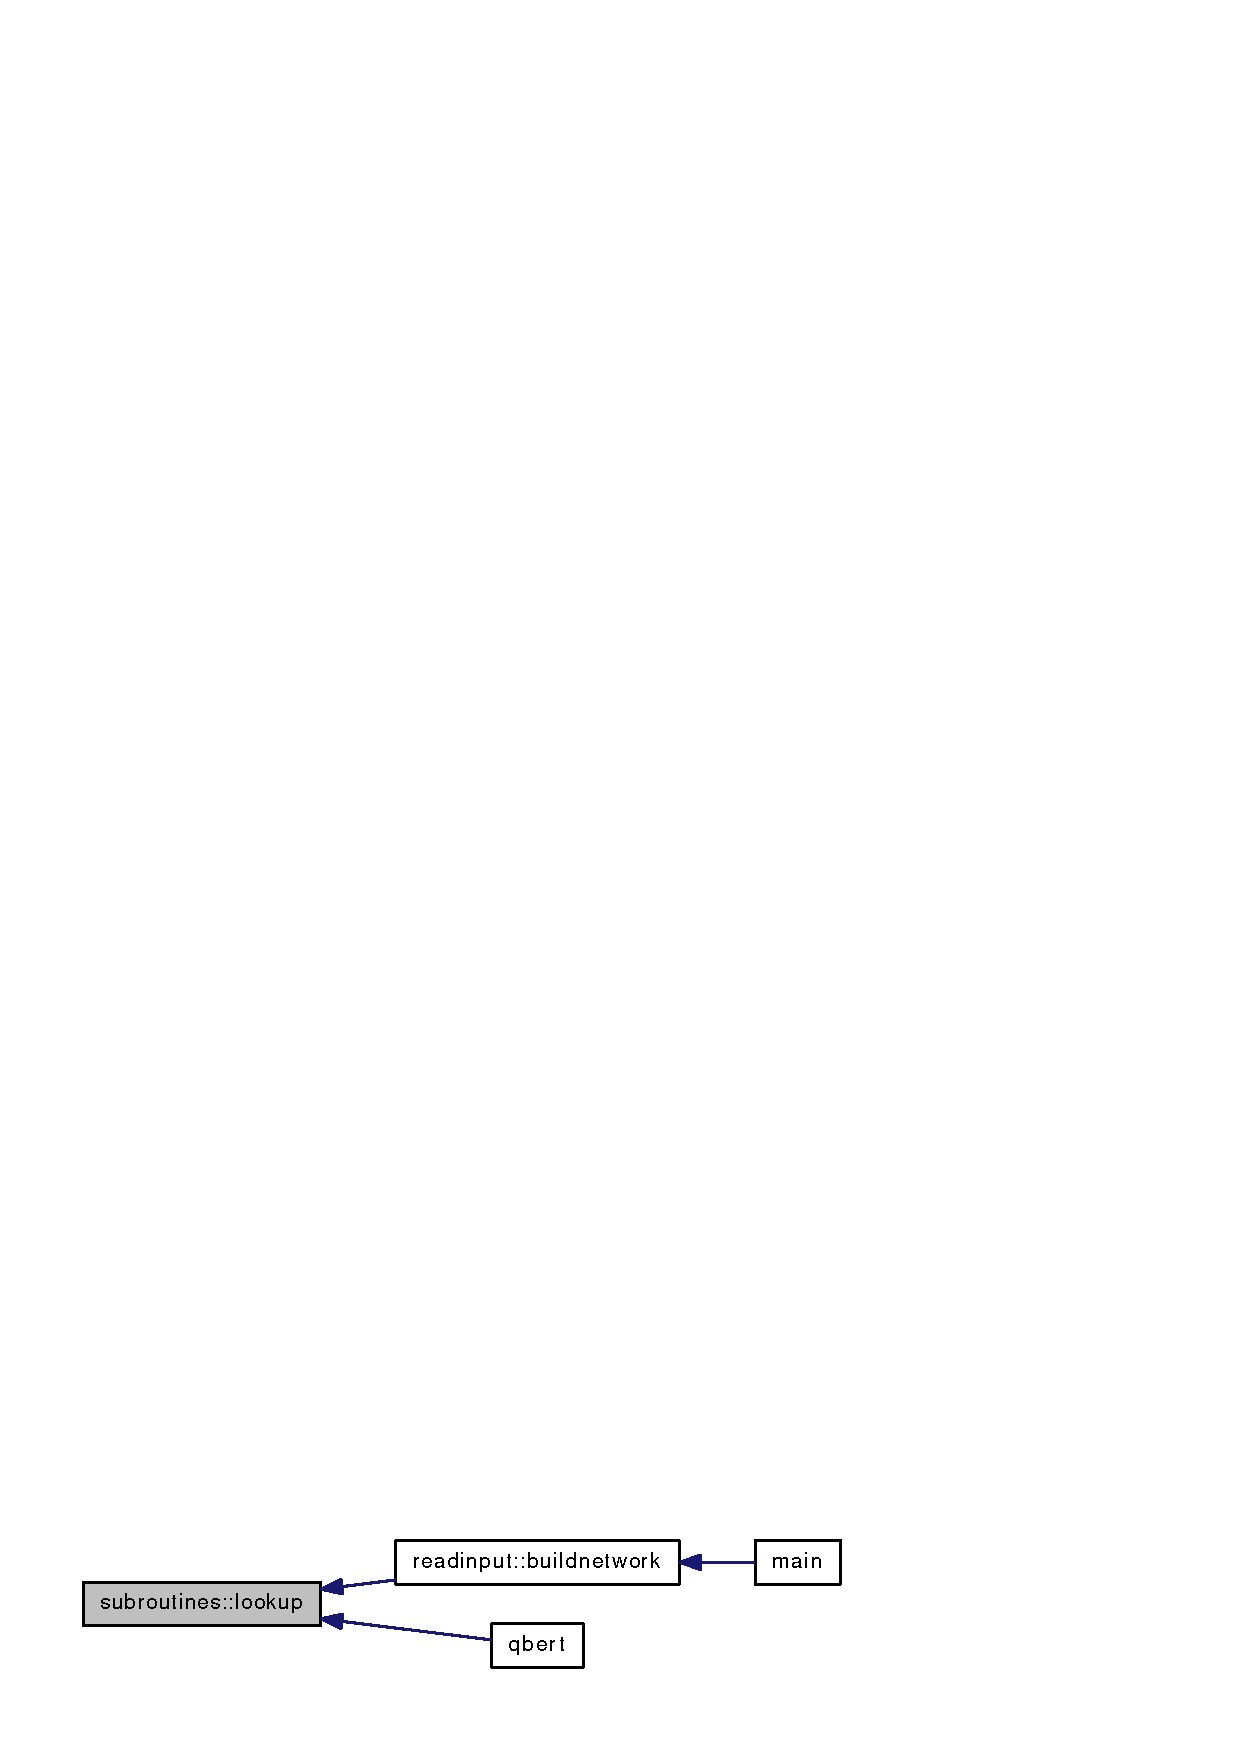
\includegraphics[width=204pt]{namespacesubroutines_a27505ee5071c93bb5f1e570995a1ac42_icgraph}
\end{center}
\end{figure}
\hypertarget{namespacesubroutines_ae942148085820c335aea6798ad4e7e7e}{
\index{subroutines@{subroutines}!new\_\-electron@{new\_\-electron}}
\index{new\_\-electron@{new\_\-electron}!subroutines@{subroutines}}
\subsubsection[{new\_\-electron}]{\setlength{\rightskip}{0pt plus 5cm}subroutine subroutines::new\_\-electron (TYPE(se\_\-info) {\em se\_\-box}, \/  TYPE(node),pointer {\em root}, \/  TYPE(node),pointer {\em temp}, \/  TYPE(node),pointer {\em prevNode}, \/  TYPE(node),pointer {\em nextNode})}}
\label{namespacesubroutines_ae942148085820c335aea6798ad4e7e7e}


Definition at line 2204 of file subroutines.f90.

References parameters::C\_\-PR, parameters::CRPNUM, parameters::DEBUG, e\_\-ex\_\-select(), e\_\-ion\_\-select(), parameters::ECUTOFF, parameters::ELECNUM, esigma\_\-suite(), parameters::EXCNUM, hopping(), parameters::IONLIST, parameters::MATRIX, new\_\-reaction(), parameters::RHO, se\_\-info\_\-garbage(), se\_\-info\_\-init(), parameters::TRACKPLOT, trackwrite(), and transport().

Referenced by fallout().

Here is the call graph for this function:\nopagebreak
\begin{figure}[H]
\begin{center}
\leavevmode
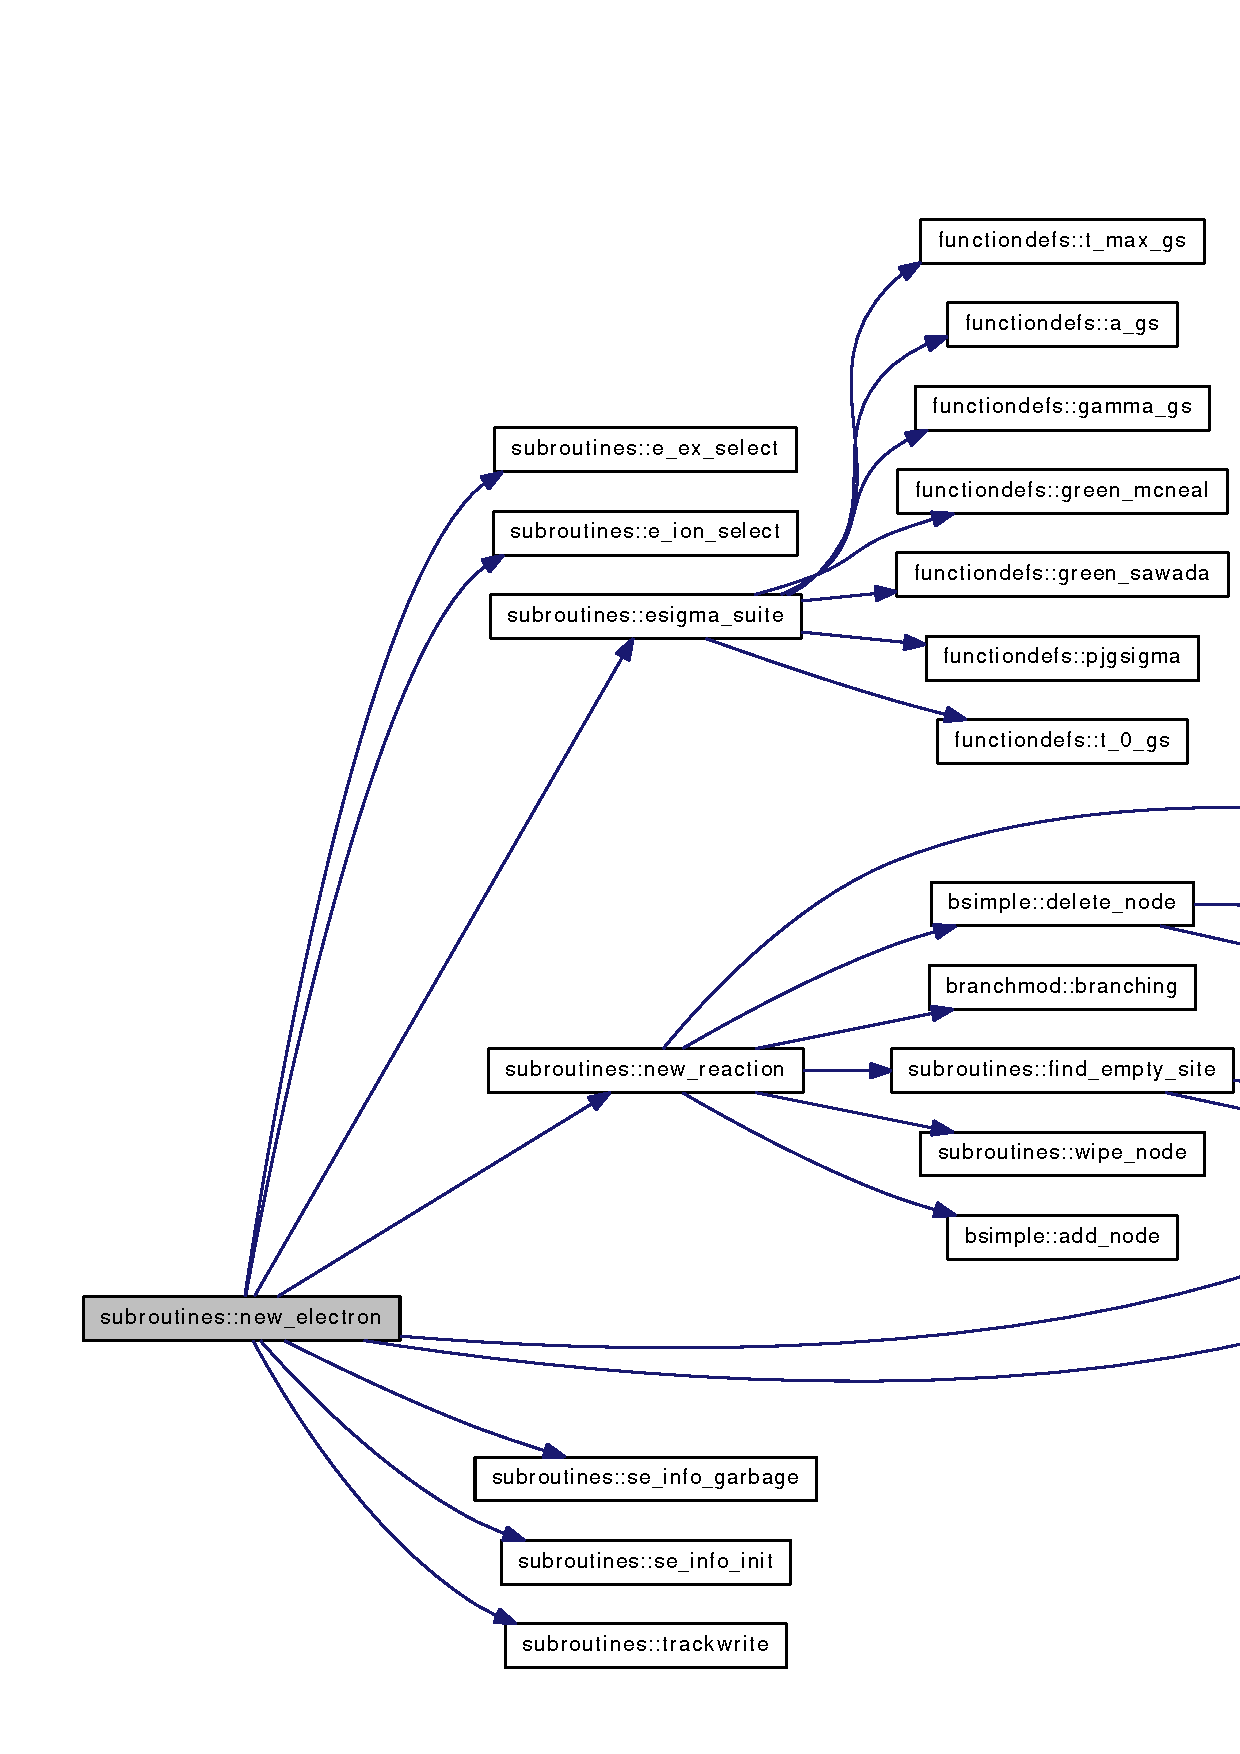
\includegraphics[width=420pt]{namespacesubroutines_ae942148085820c335aea6798ad4e7e7e_cgraph}
\end{center}
\end{figure}


Here is the caller graph for this function:\nopagebreak
\begin{figure}[H]
\begin{center}
\leavevmode
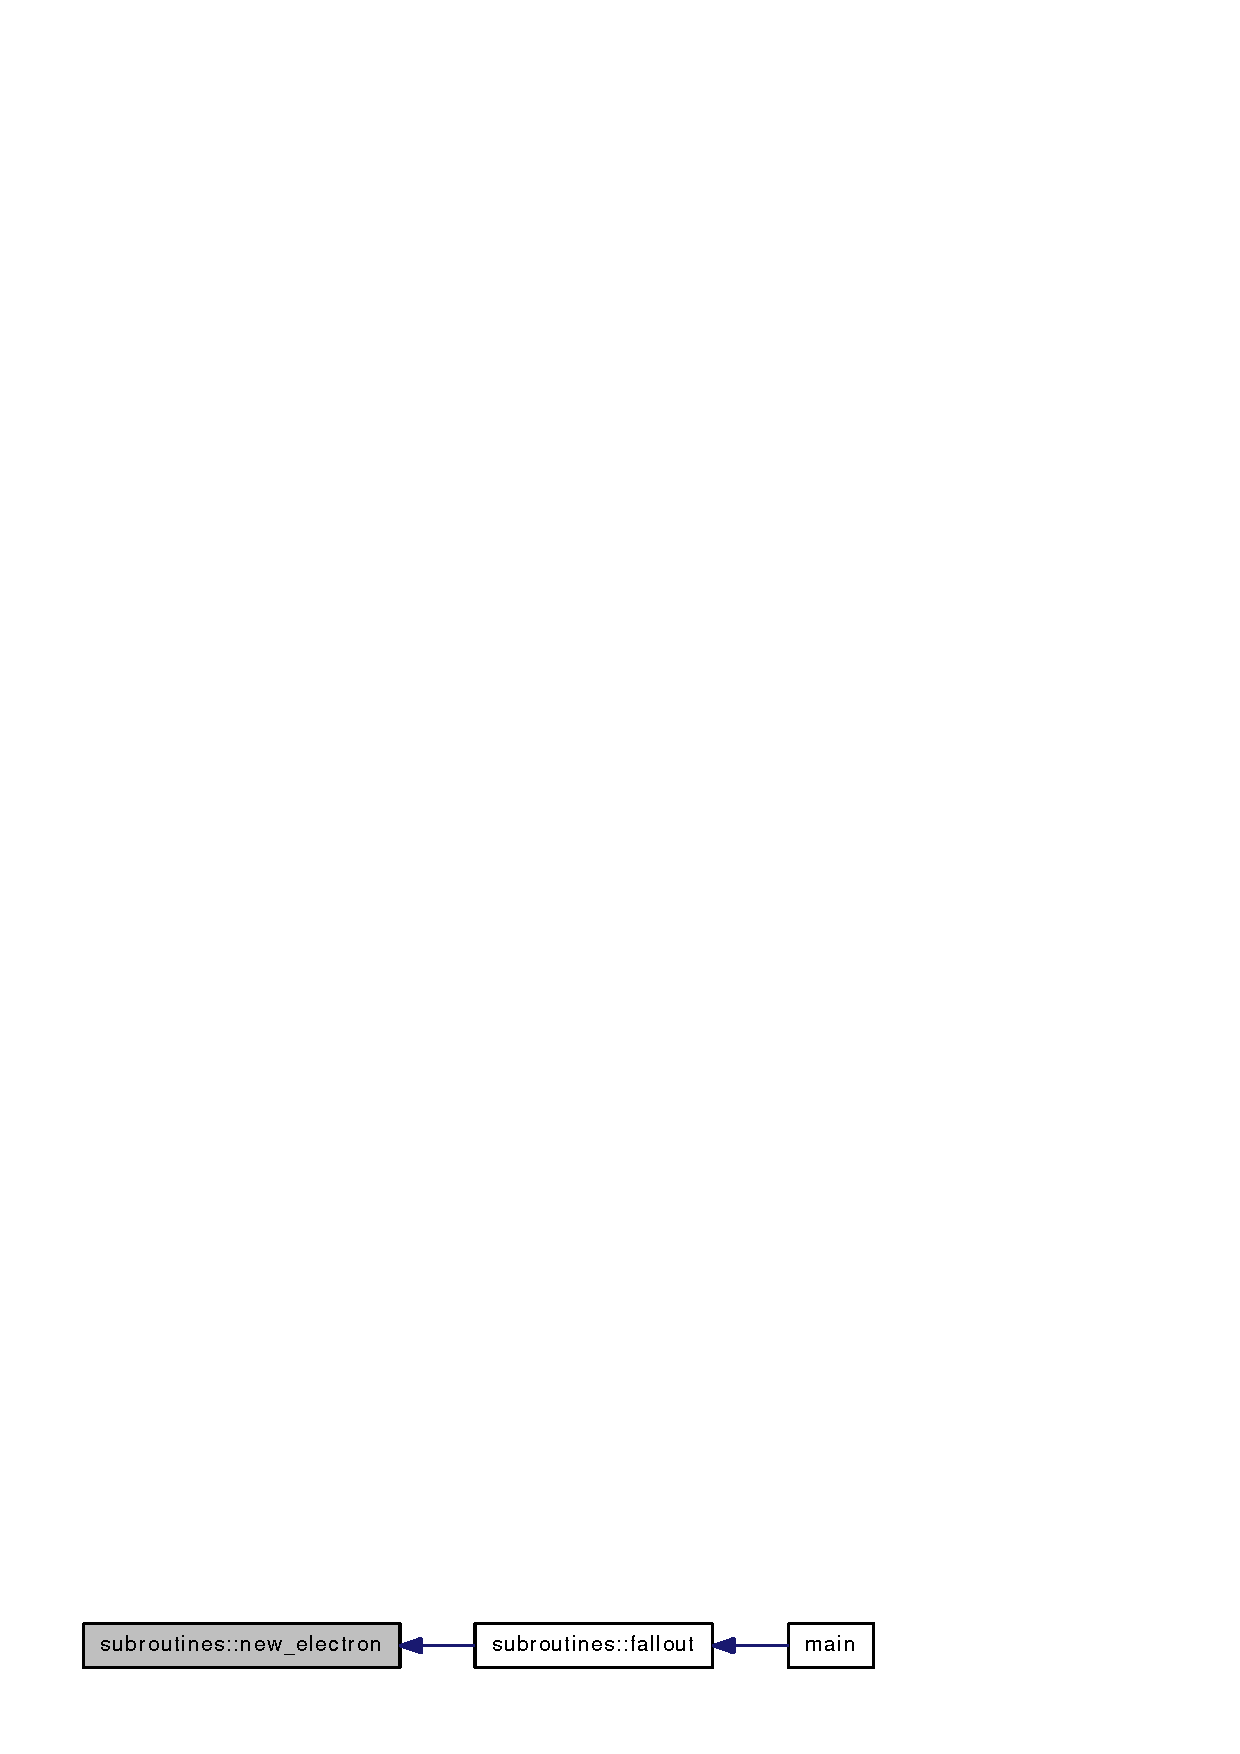
\includegraphics[width=212pt]{namespacesubroutines_ae942148085820c335aea6798ad4e7e7e_icgraph}
\end{center}
\end{figure}
\hypertarget{namespacesubroutines_a5f9a688681311ebc691561ec51015d0f}{
\index{subroutines@{subroutines}!new\_\-reaction@{new\_\-reaction}}
\index{new\_\-reaction@{new\_\-reaction}!subroutines@{subroutines}}
\subsubsection[{new\_\-reaction}]{\setlength{\rightskip}{0pt plus 5cm}subroutine subroutines::new\_\-reaction (INTEGER,dimension(3),intent(inout) {\em i}, \/  INTEGER,dimension(3),intent(inout) {\em j}, \/  INTEGER,dimension(3),intent(inout) {\em k}, \/  TYPE(node),pointer {\em root}, \/  TYPE(node),pointer {\em temp}, \/  TYPE(node),pointer {\em prevNode}, \/  TYPE(node),pointer {\em nextNode}, \/  INTEGER {\em error})}}
\label{namespacesubroutines_a5f9a688681311ebc691561ec51015d0f}


Definition at line 2049 of file subroutines.f90.

References bsimple::add\_\-node(), branchmod::branching(), parameters::DEBUG, bsimple::delete\_\-node(), parameters::ELECNUM, find\_\-empty\_\-site(), parameters::ISBARRIER, parameters::MATRIX, parameters::SPECIAL\_\-LIST, wait\_\-calc(), and wipe\_\-node().

Referenced by fallout(), main(), and new\_\-electron().

Here is the call graph for this function:\nopagebreak
\begin{figure}[H]
\begin{center}
\leavevmode
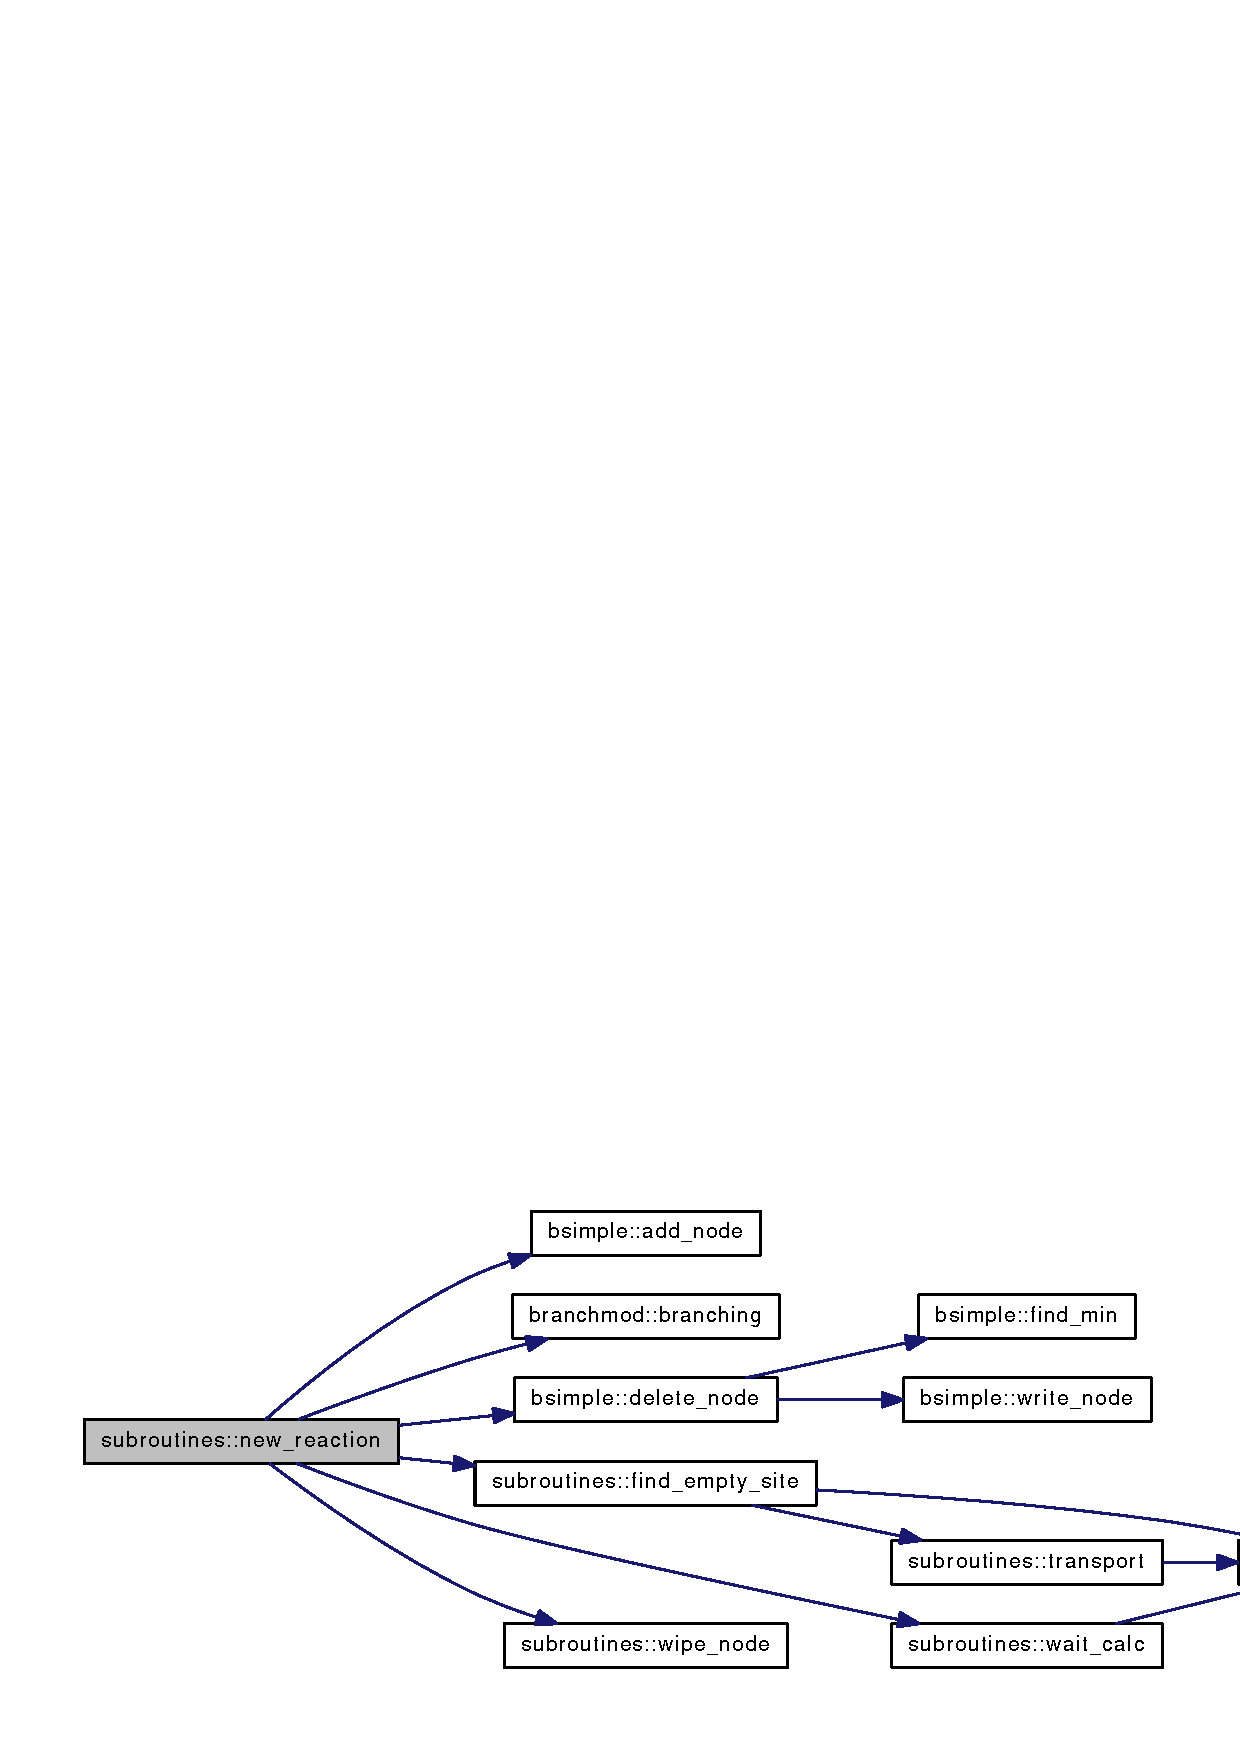
\includegraphics[width=360pt]{namespacesubroutines_a5f9a688681311ebc691561ec51015d0f_cgraph}
\end{center}
\end{figure}


Here is the caller graph for this function:\nopagebreak
\begin{figure}[H]
\begin{center}
\leavevmode
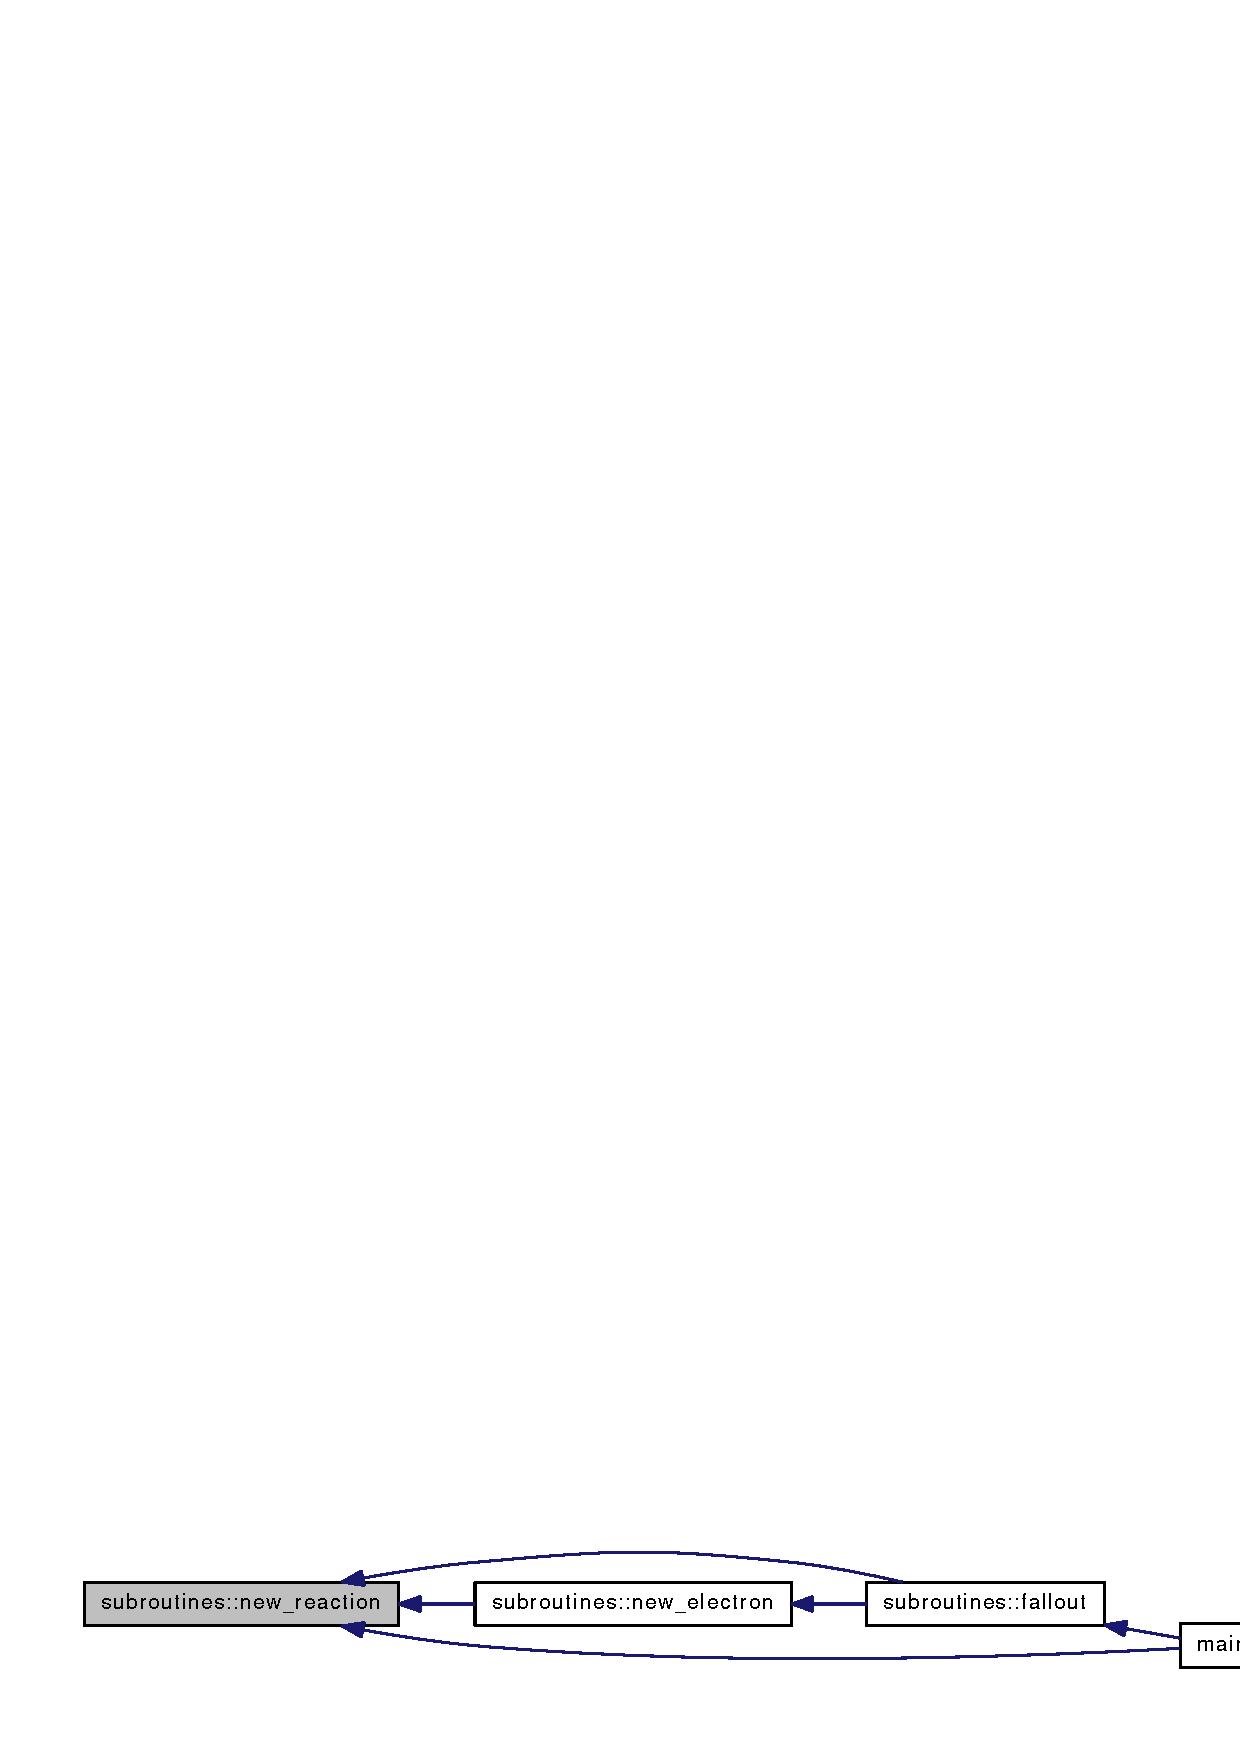
\includegraphics[width=306pt]{namespacesubroutines_a5f9a688681311ebc691561ec51015d0f_icgraph}
\end{center}
\end{figure}
\hypertarget{namespacesubroutines_acad706394e0b01bbd1e5345585dace59}{
\index{subroutines@{subroutines}!p\_\-ex\_\-select@{p\_\-ex\_\-select}}
\index{p\_\-ex\_\-select@{p\_\-ex\_\-select}!subroutines@{subroutines}}
\subsubsection[{p\_\-ex\_\-select}]{\setlength{\rightskip}{0pt plus 5cm}subroutine subroutines::p\_\-ex\_\-select (DOUBLE PRECISION,dimension(:),pointer {\em psigexj}, \/  DOUBLE PRECISION,intent(out) {\em e\_\-exc}, \/  INTEGER,intent(in) {\em thinghit})}}
\label{namespacesubroutines_acad706394e0b01bbd1e5345585dace59}


Definition at line 1544 of file subroutines.f90.

References specdata::o2\_\-p\_\-ex, specdata::o3\_\-p\_\-ex, parameters::O3NUM, parameters::O3STARNUM, specdata::o\_\-p\_\-ex, parameters::ONUM, and parameters::OSTARNUM.

Referenced by fallout().

Here is the caller graph for this function:\nopagebreak
\begin{figure}[H]
\begin{center}
\leavevmode
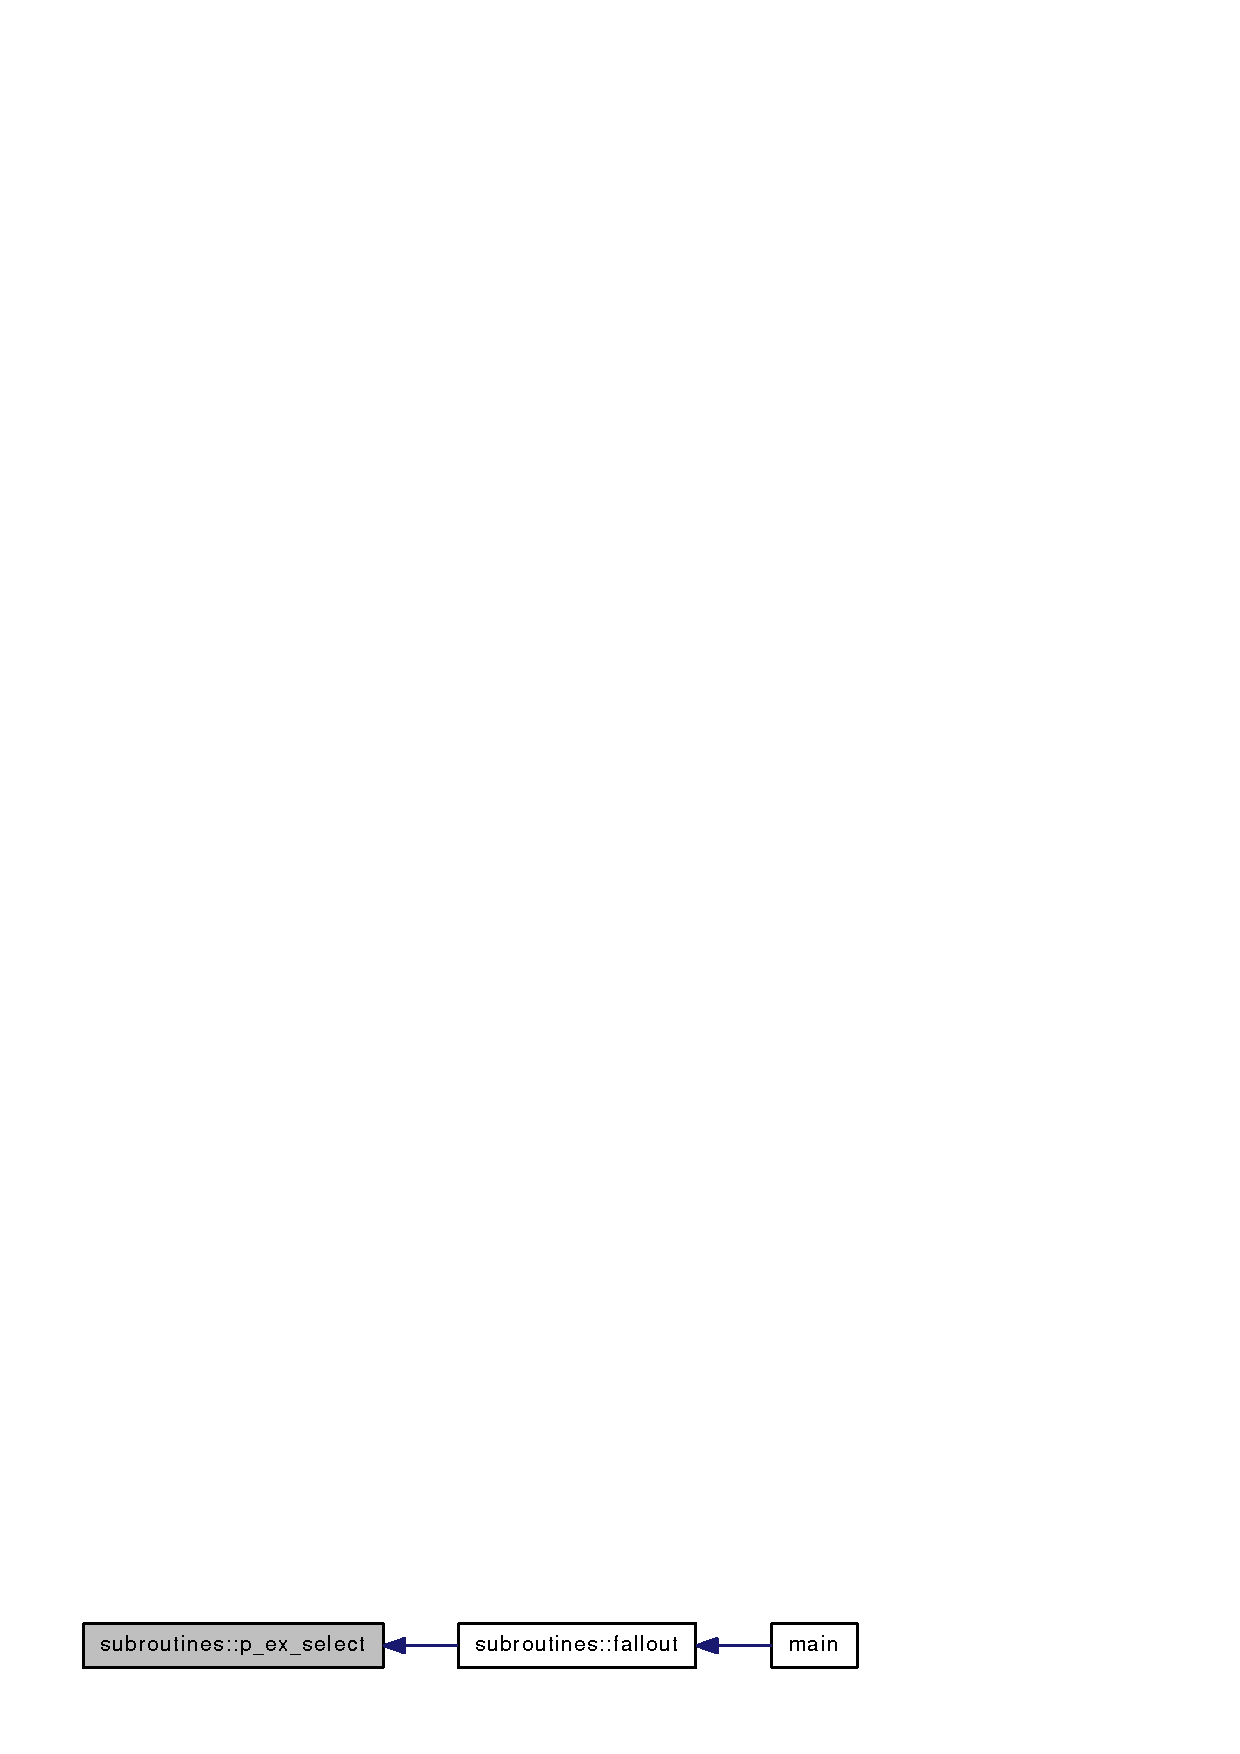
\includegraphics[width=208pt]{namespacesubroutines_acad706394e0b01bbd1e5345585dace59_icgraph}
\end{center}
\end{figure}
\hypertarget{namespacesubroutines_a3185cd857374fa3b0a19f2a56e6474df}{
\index{subroutines@{subroutines}!p\_\-ion\_\-select@{p\_\-ion\_\-select}}
\index{p\_\-ion\_\-select@{p\_\-ion\_\-select}!subroutines@{subroutines}}
\subsubsection[{p\_\-ion\_\-select}]{\setlength{\rightskip}{0pt plus 5cm}subroutine subroutines::p\_\-ion\_\-select (DOUBLE PRECISION,dimension(:),pointer {\em psigij}, \/  DOUBLE PRECISION,intent(out) {\em e\_\-ion}, \/  DOUBLE PRECISION,intent(out) {\em e\_\-se}, \/  INTEGER,intent(in) {\em thinghit})}}
\label{namespacesubroutines_a3185cd857374fa3b0a19f2a56e6474df}


Definition at line 1479 of file subroutines.f90.

References parameters::AVAL, specdata::o2\_\-p\_\-ion, specdata::o3\_\-p\_\-ion, parameters::O3NUM, parameters::O3STARNUM, specdata::o\_\-p\_\-ion, parameters::ONUM, parameters::OSTARNUM, and mc\_\-toolbox::rgamma().

Referenced by fallout().

Here is the call graph for this function:\nopagebreak
\begin{figure}[H]
\begin{center}
\leavevmode
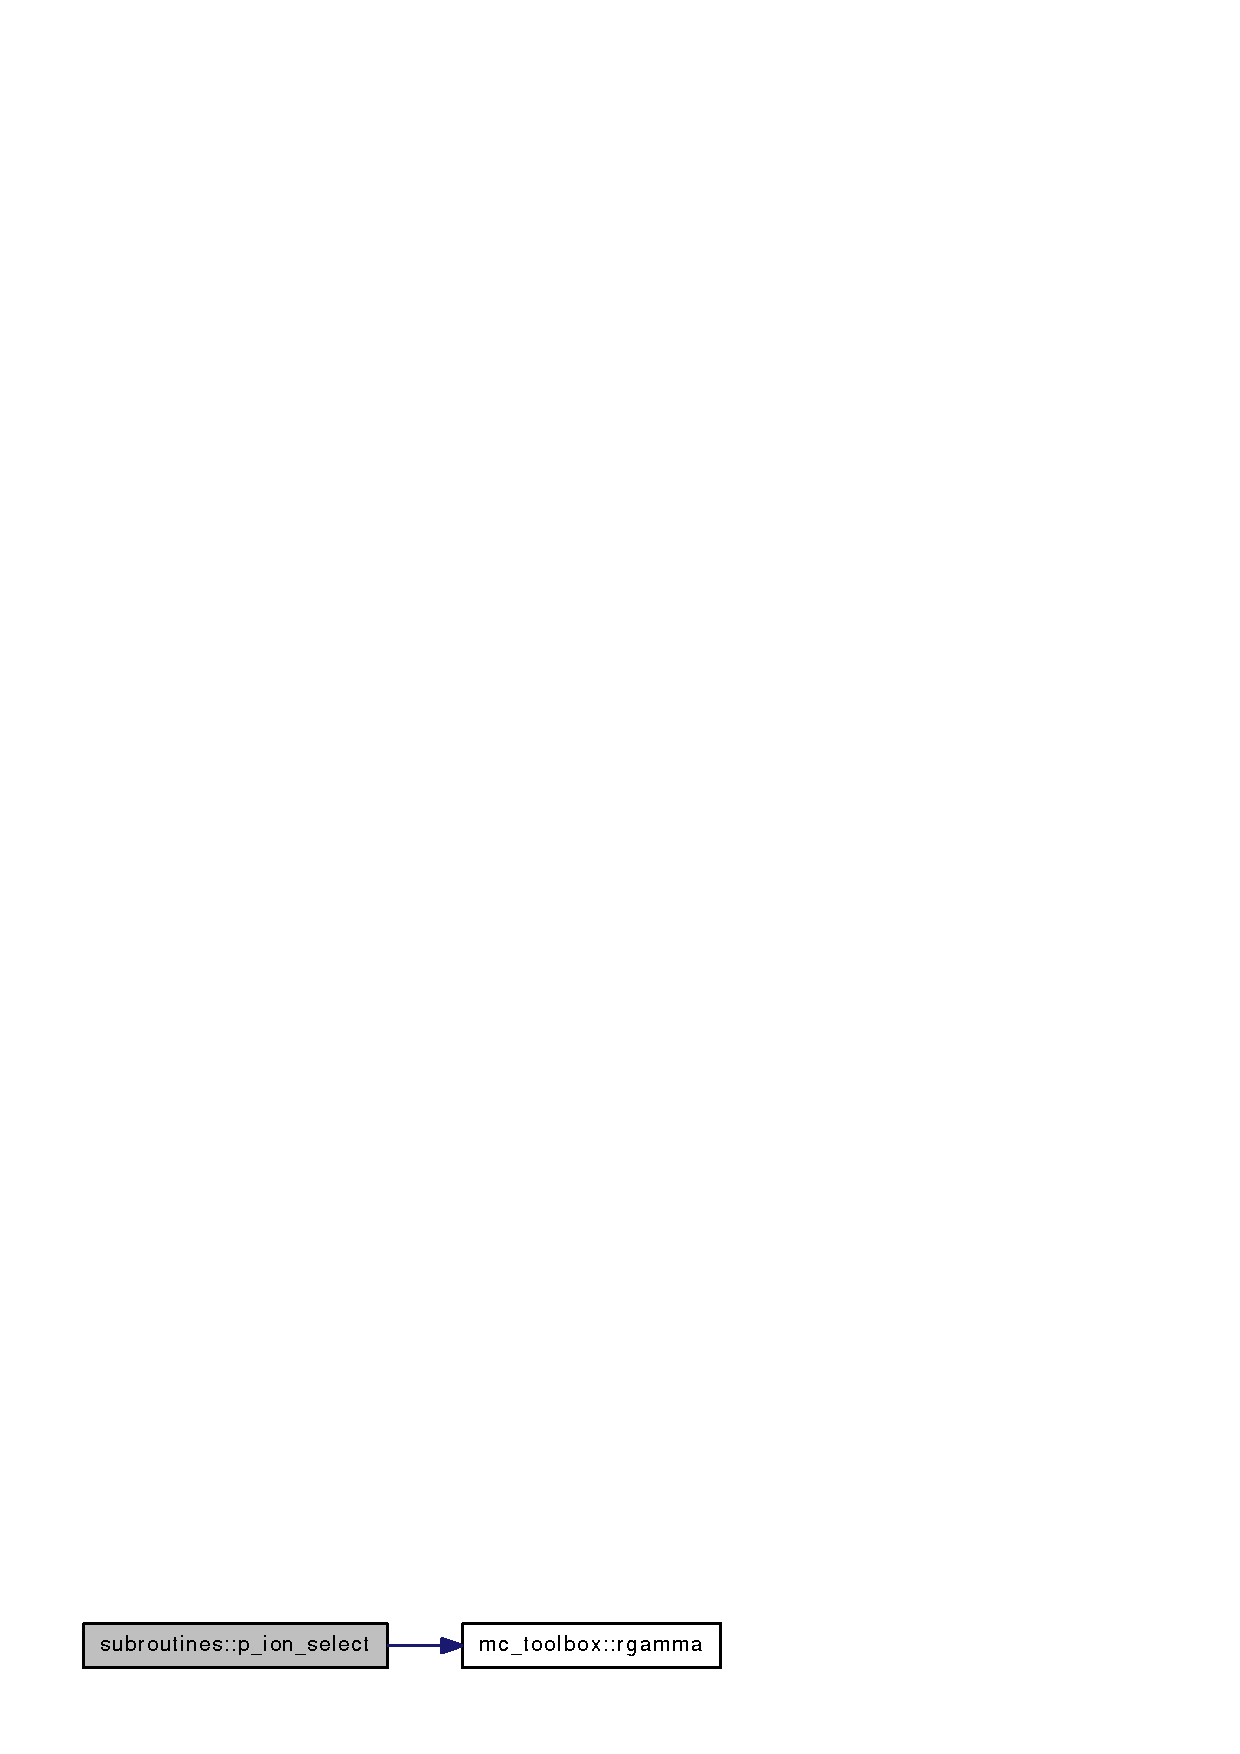
\includegraphics[width=175pt]{namespacesubroutines_a3185cd857374fa3b0a19f2a56e6474df_cgraph}
\end{center}
\end{figure}


Here is the caller graph for this function:\nopagebreak
\begin{figure}[H]
\begin{center}
\leavevmode
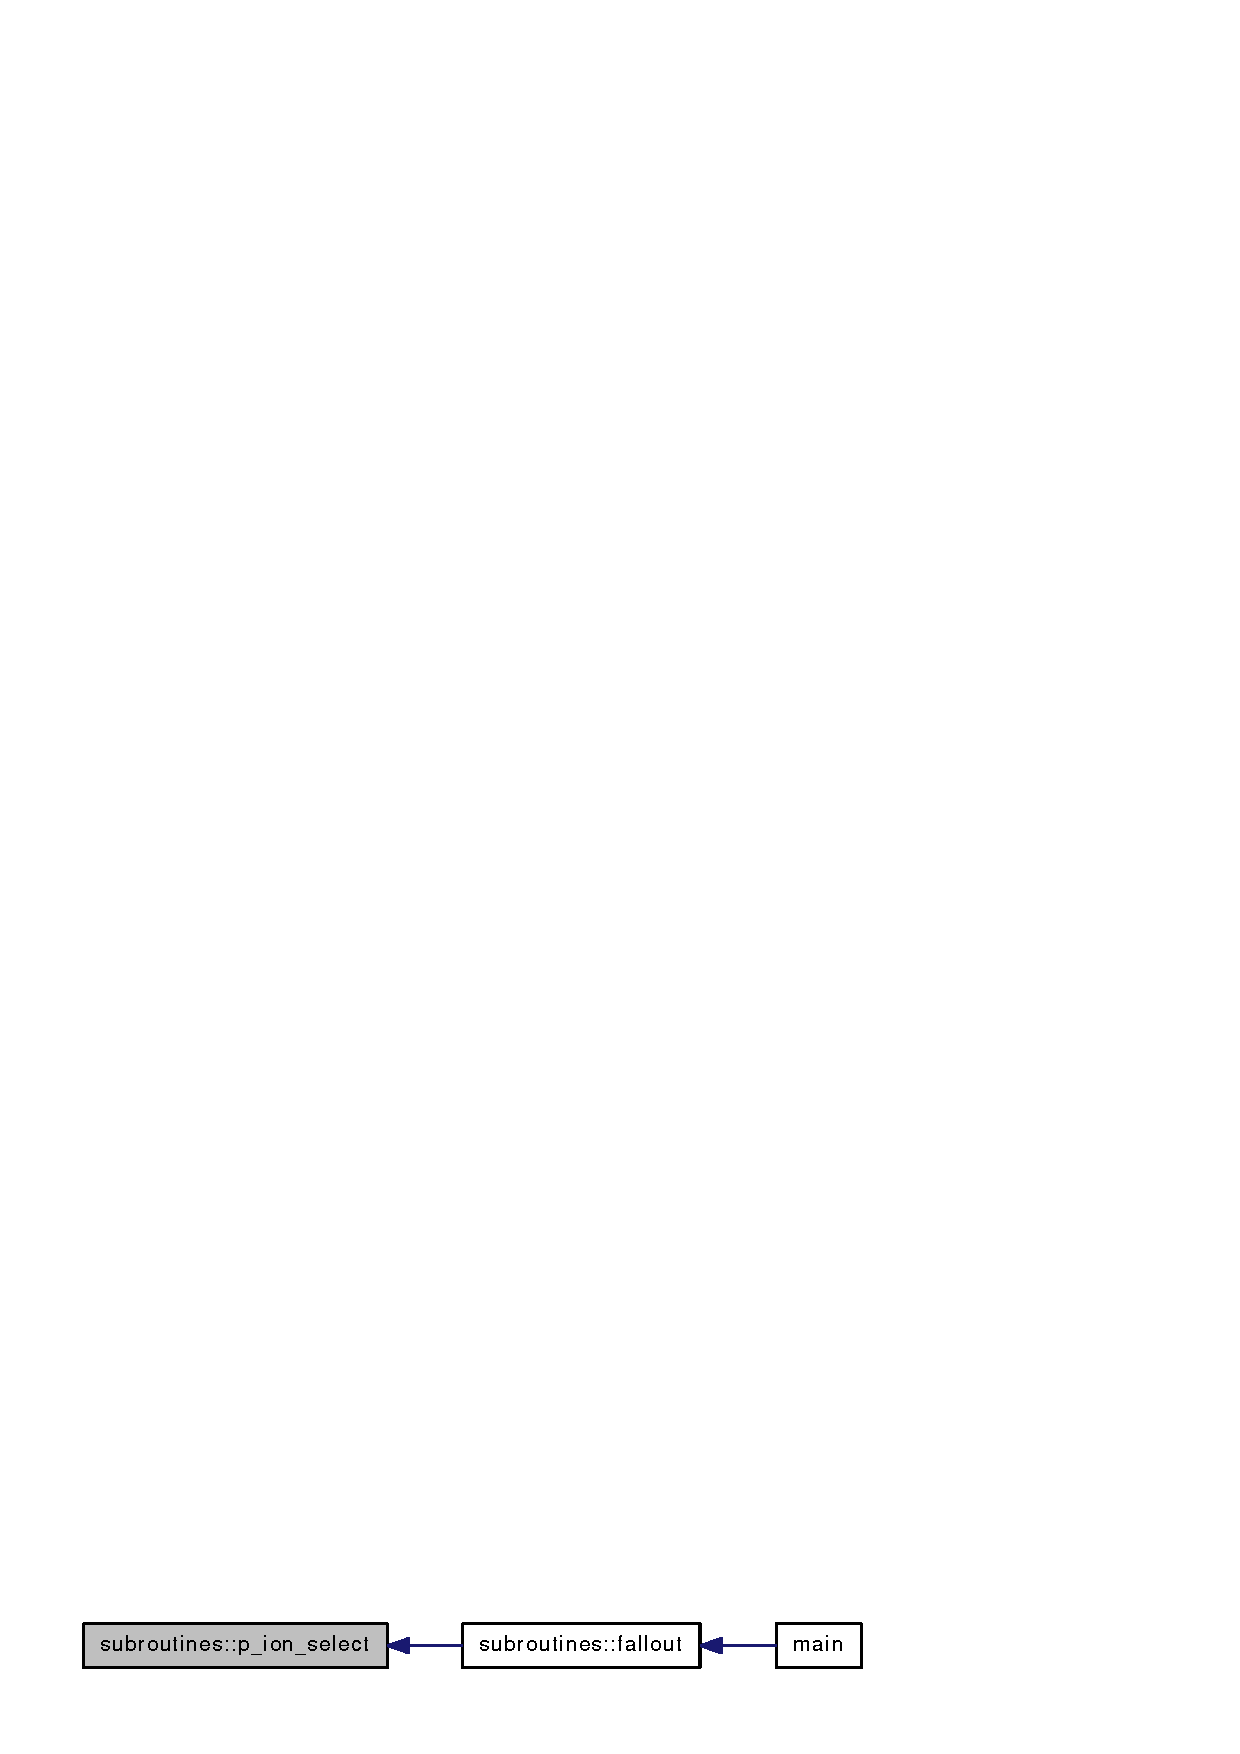
\includegraphics[width=209pt]{namespacesubroutines_a3185cd857374fa3b0a19f2a56e6474df_icgraph}
\end{center}
\end{figure}
\hypertarget{namespacesubroutines_a37b9d3b519b164f5ef3835bf4e1e4f8c}{
\index{subroutines@{subroutines}!psigma\_\-suite@{psigma\_\-suite}}
\index{psigma\_\-suite@{psigma\_\-suite}!subroutines@{subroutines}}
\subsubsection[{psigma\_\-suite}]{\setlength{\rightskip}{0pt plus 5cm}subroutine subroutines::psigma\_\-suite (DOUBLE PRECISION,pointer {\em energy}, \/  TYPE(SIGMA\_\-BOX),dimension(:),pointer {\em psigmas}, \/  DOUBLE PRECISION,dimension(:),pointer {\em psigij}, \/  DOUBLE PRECISION,dimension(:),pointer {\em psigexj}, \/  TYPE(SIGMA\_\-BOX),dimension(:),pointer {\em o\_\-psigmas}, \/  DOUBLE PRECISION,dimension(:),pointer {\em o\_\-psigij}, \/  DOUBLE PRECISION,dimension(:),pointer {\em o\_\-psigexj}, \/  TYPE(SIGMA\_\-BOX),dimension(:),pointer {\em o3\_\-psigmas}, \/  DOUBLE PRECISION,dimension(:),pointer {\em o3\_\-psigij}, \/  DOUBLE PRECISION,dimension(:),pointer {\em o3\_\-psigexj})}}
\label{namespacesubroutines_a37b9d3b519b164f5ef3835bf4e1e4f8c}


Definition at line 1089 of file subroutines.f90.

References functiondefs::au(), functiondefs::eps(), functiondefs::green\_\-mcneal(), functiondefs::mass\_\-fac(), parameters::MO1, parameters::MO2, parameters::MO3, parameters::MP, specdata::o2\_\-p\_\-ex, specdata::o2\_\-p\_\-ion, specdata::o3\_\-p\_\-ex, specdata::o3\_\-p\_\-ion, specdata::o\_\-p\_\-ex, specdata::o\_\-p\_\-ion, functiondefs::pelsig(), functiondefs::sne(), functiondefs::sneps(), parameters::ZO1, parameters::ZO2, parameters::ZO3, and parameters::ZP.

Referenced by fallout(), and sigma\_\-test().

Here is the call graph for this function:\nopagebreak
\begin{figure}[H]
\begin{center}
\leavevmode
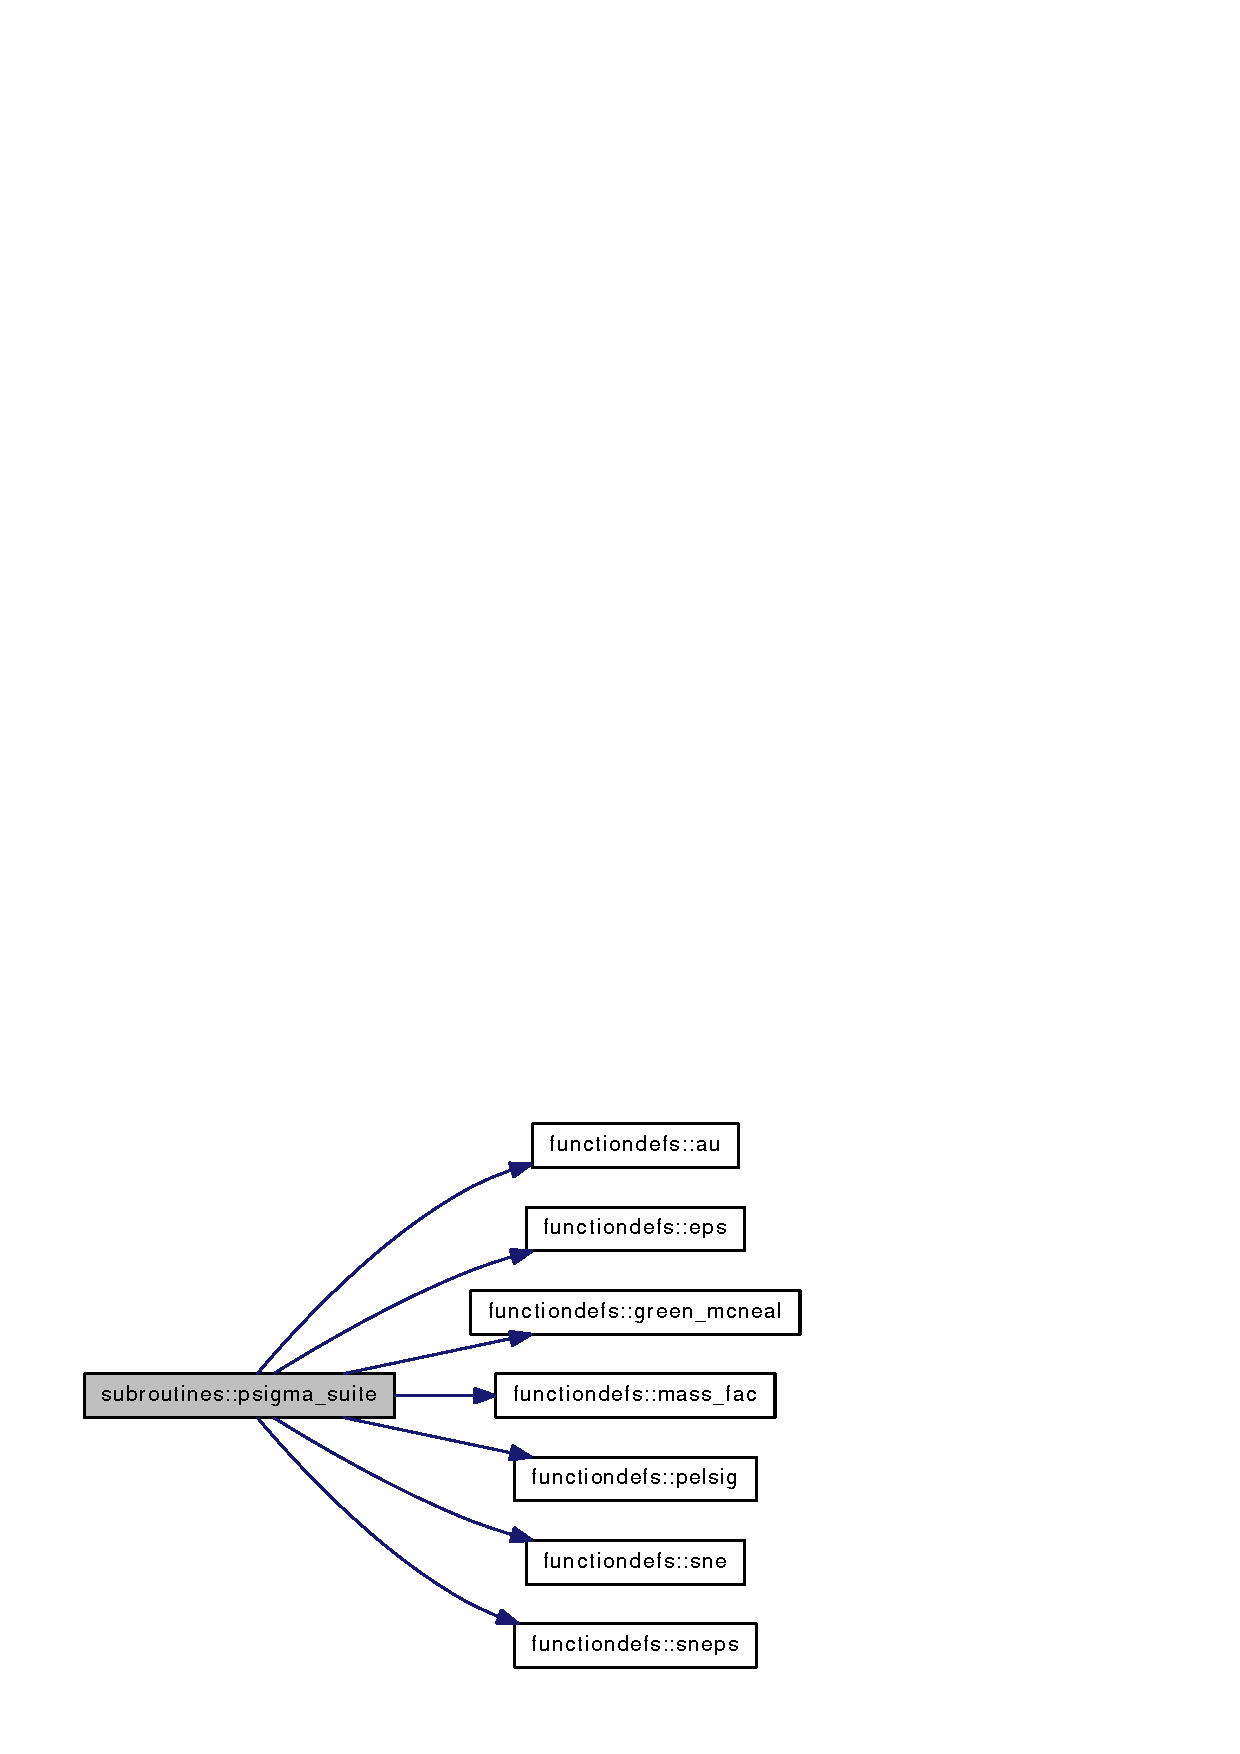
\includegraphics[width=194pt]{namespacesubroutines_a37b9d3b519b164f5ef3835bf4e1e4f8c_cgraph}
\end{center}
\end{figure}


Here is the caller graph for this function:\nopagebreak
\begin{figure}[H]
\begin{center}
\leavevmode
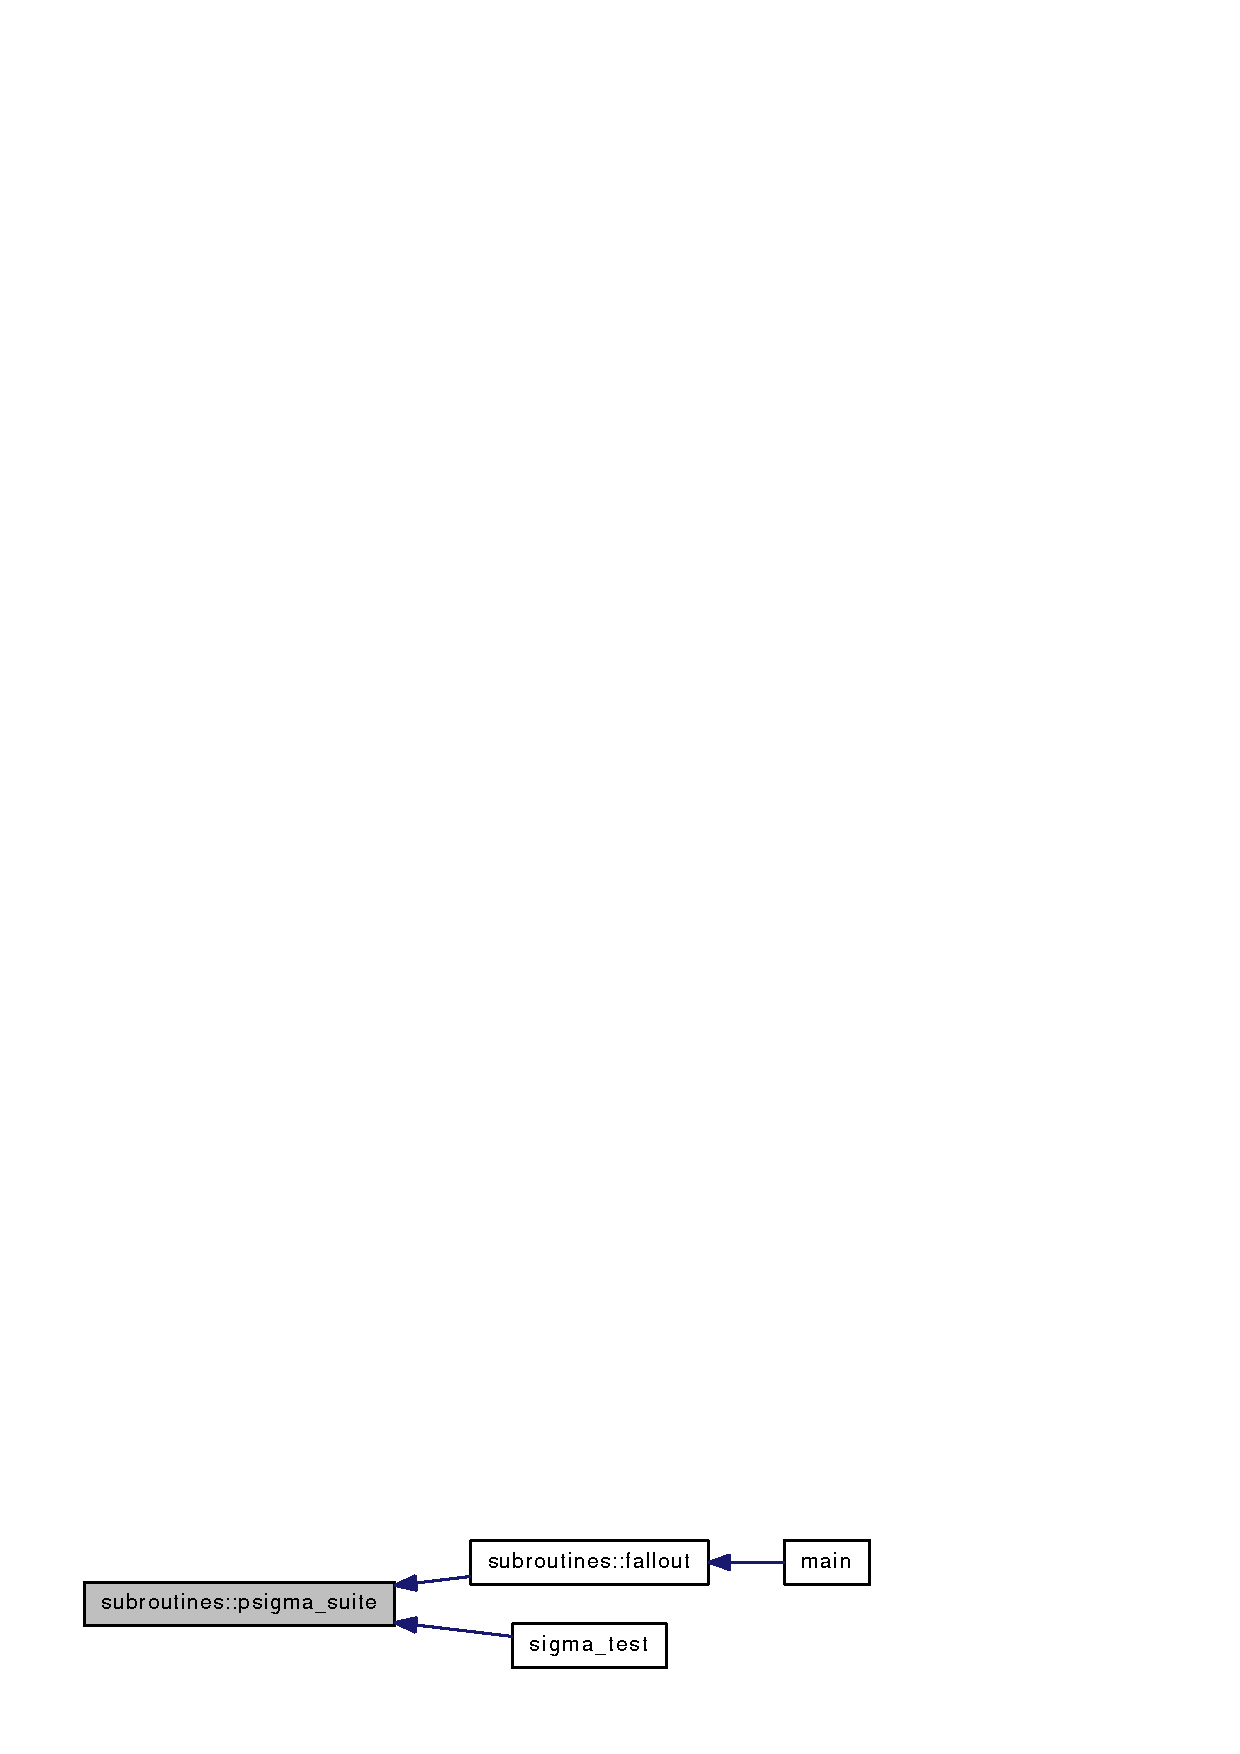
\includegraphics[width=211pt]{namespacesubroutines_a37b9d3b519b164f5ef3835bf4e1e4f8c_icgraph}
\end{center}
\end{figure}
\hypertarget{namespacesubroutines_a1d1775ee81394d8c078c760678a530e2}{
\index{subroutines@{subroutines}!se\_\-info\_\-garbage@{se\_\-info\_\-garbage}}
\index{se\_\-info\_\-garbage@{se\_\-info\_\-garbage}!subroutines@{subroutines}}
\subsubsection[{se\_\-info\_\-garbage}]{\setlength{\rightskip}{0pt plus 5cm}subroutine subroutines::se\_\-info\_\-garbage (TYPE(se\_\-info) {\em se\_\-box})}}
\label{namespacesubroutines_a1d1775ee81394d8c078c760678a530e2}


Definition at line 1956 of file subroutines.f90.

Referenced by fallout(), and new\_\-electron().

Here is the caller graph for this function:\nopagebreak
\begin{figure}[H]
\begin{center}
\leavevmode
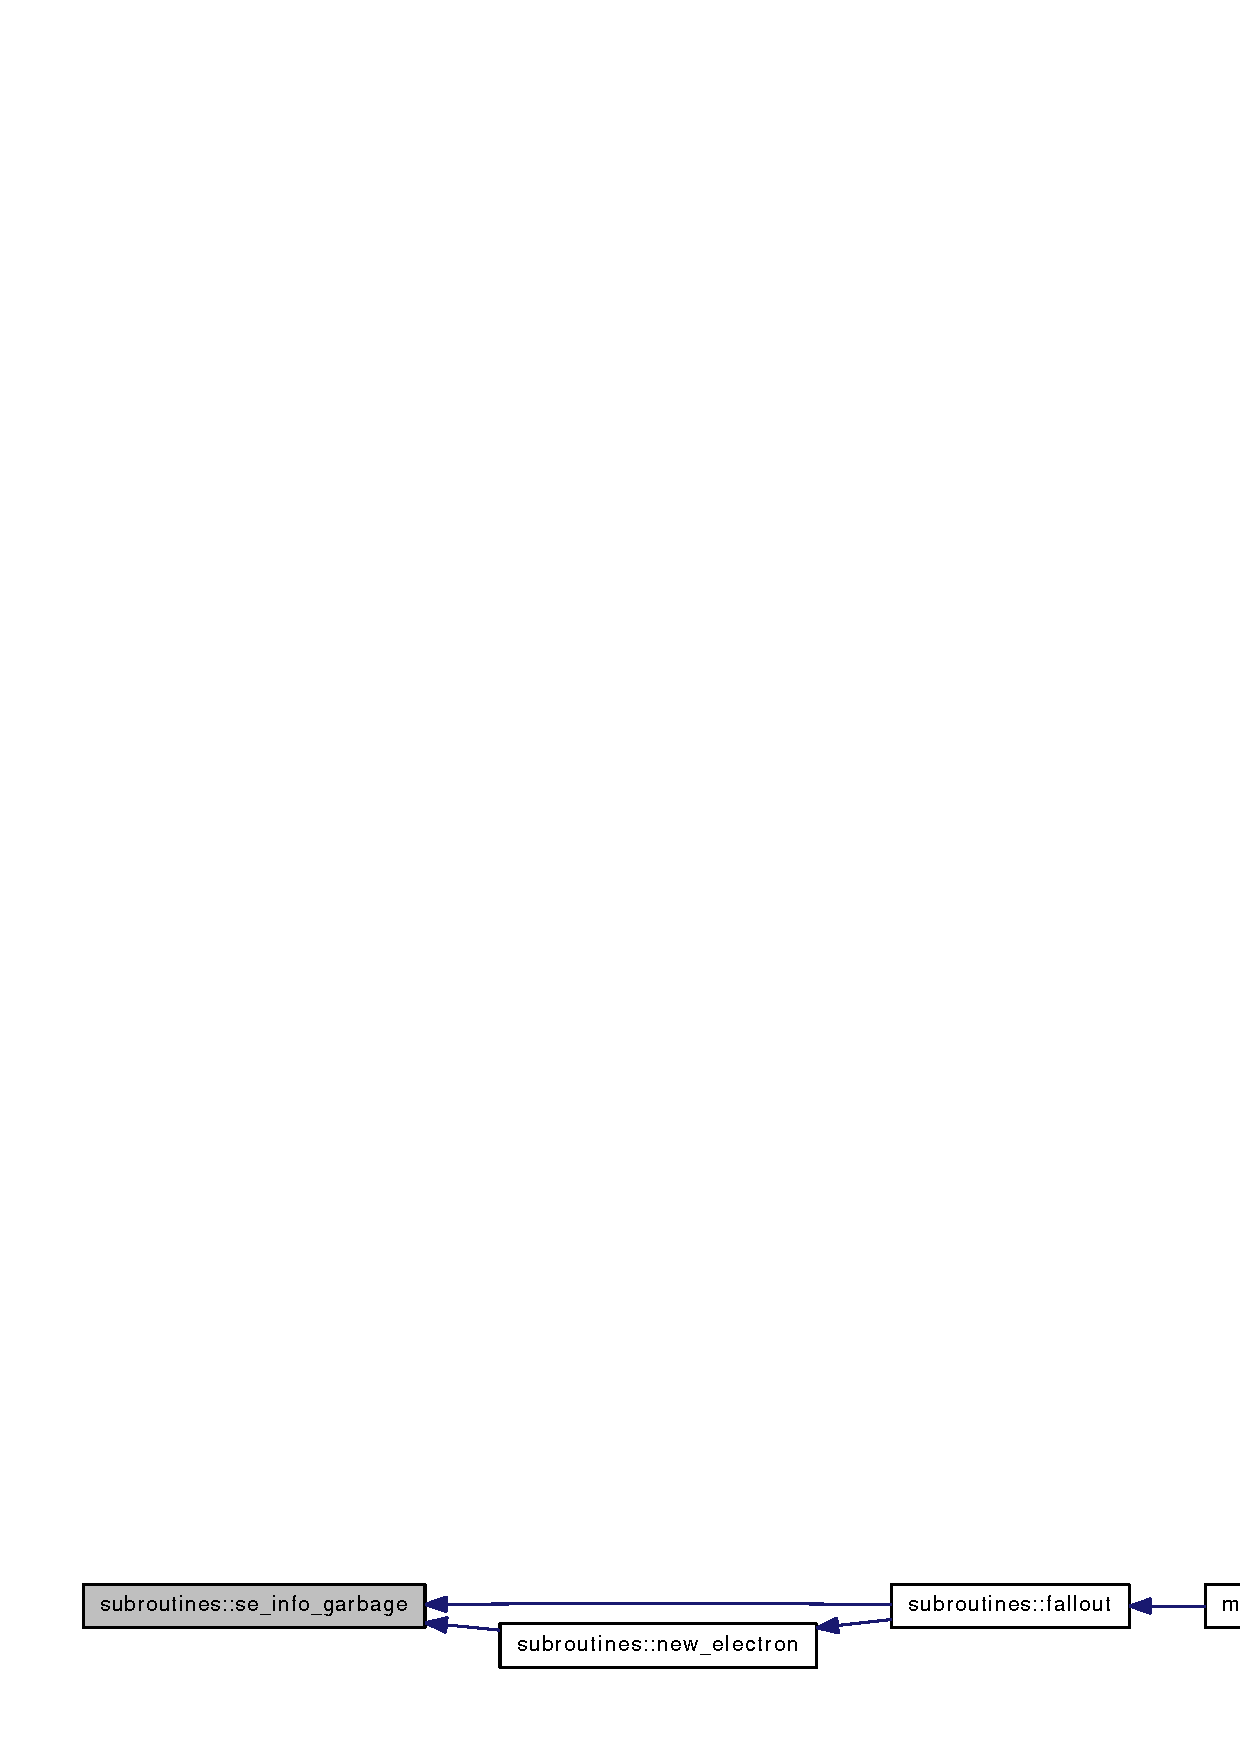
\includegraphics[width=312pt]{namespacesubroutines_a1d1775ee81394d8c078c760678a530e2_icgraph}
\end{center}
\end{figure}
\hypertarget{namespacesubroutines_aece587c9d144811189bd1ccf8a59f189}{
\index{subroutines@{subroutines}!se\_\-info\_\-init@{se\_\-info\_\-init}}
\index{se\_\-info\_\-init@{se\_\-info\_\-init}!subroutines@{subroutines}}
\subsubsection[{se\_\-info\_\-init}]{\setlength{\rightskip}{0pt plus 5cm}subroutine subroutines::se\_\-info\_\-init (TYPE(se\_\-info) {\em se\_\-box})}}
\label{namespacesubroutines_aece587c9d144811189bd1ccf8a59f189}


Definition at line 1887 of file subroutines.f90.

References specdata::o2\_\-e\_\-ex\_\-alwd, specdata::o2\_\-e\_\-ex\_\-fbdn, specdata::o2\_\-e\_\-ion, specdata::o\_\-e\_\-ex\_\-alwd, specdata::o\_\-e\_\-ex\_\-fbdn, and specdata::o\_\-e\_\-ion.

Referenced by fallout(), new\_\-electron(), and sigma\_\-test().

Here is the caller graph for this function:\nopagebreak
\begin{figure}[H]
\begin{center}
\leavevmode
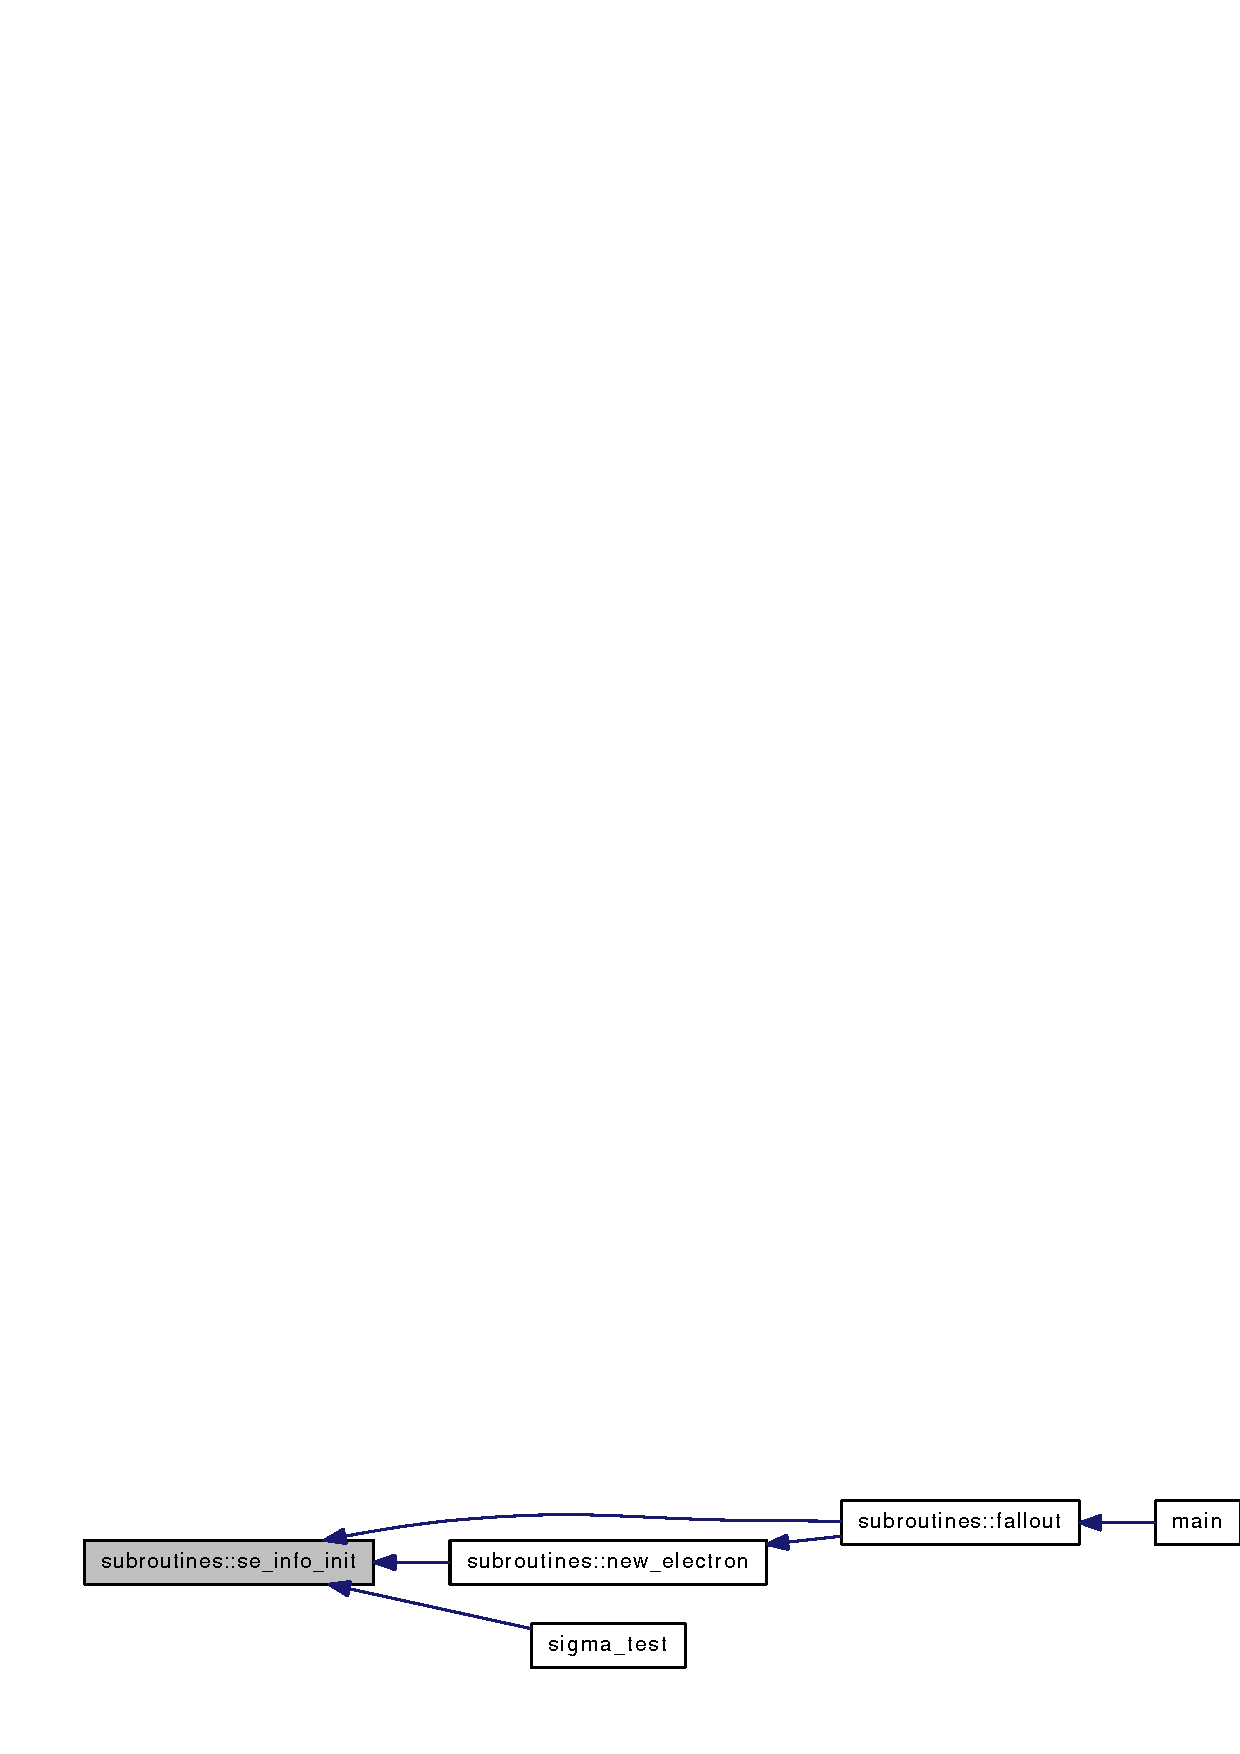
\includegraphics[width=300pt]{namespacesubroutines_aece587c9d144811189bd1ccf8a59f189_icgraph}
\end{center}
\end{figure}
\hypertarget{namespacesubroutines_abbce0f7ec92c43ac91db25f512531642}{
\index{subroutines@{subroutines}!trackwrite@{trackwrite}}
\index{trackwrite@{trackwrite}!subroutines@{subroutines}}
\subsubsection[{trackwrite}]{\setlength{\rightskip}{0pt plus 5cm}subroutine subroutines::trackwrite (INTEGER,dimension(:),intent(in) {\em coords}, \/  DOUBLE PRECISION,intent(in) {\em energy}, \/  INTEGER,intent(in) {\em e\_\-branch}, \/  LOGICAL,intent(in) {\em electron})}}
\label{namespacesubroutines_abbce0f7ec92c43ac91db25f512531642}


Definition at line 2500 of file subroutines.f90.

References parameters::PMODEL, and parameters::TRACKPLOT\_\-LUN.

Referenced by fallout(), and new\_\-electron().

Here is the caller graph for this function:\nopagebreak
\begin{figure}[H]
\begin{center}
\leavevmode
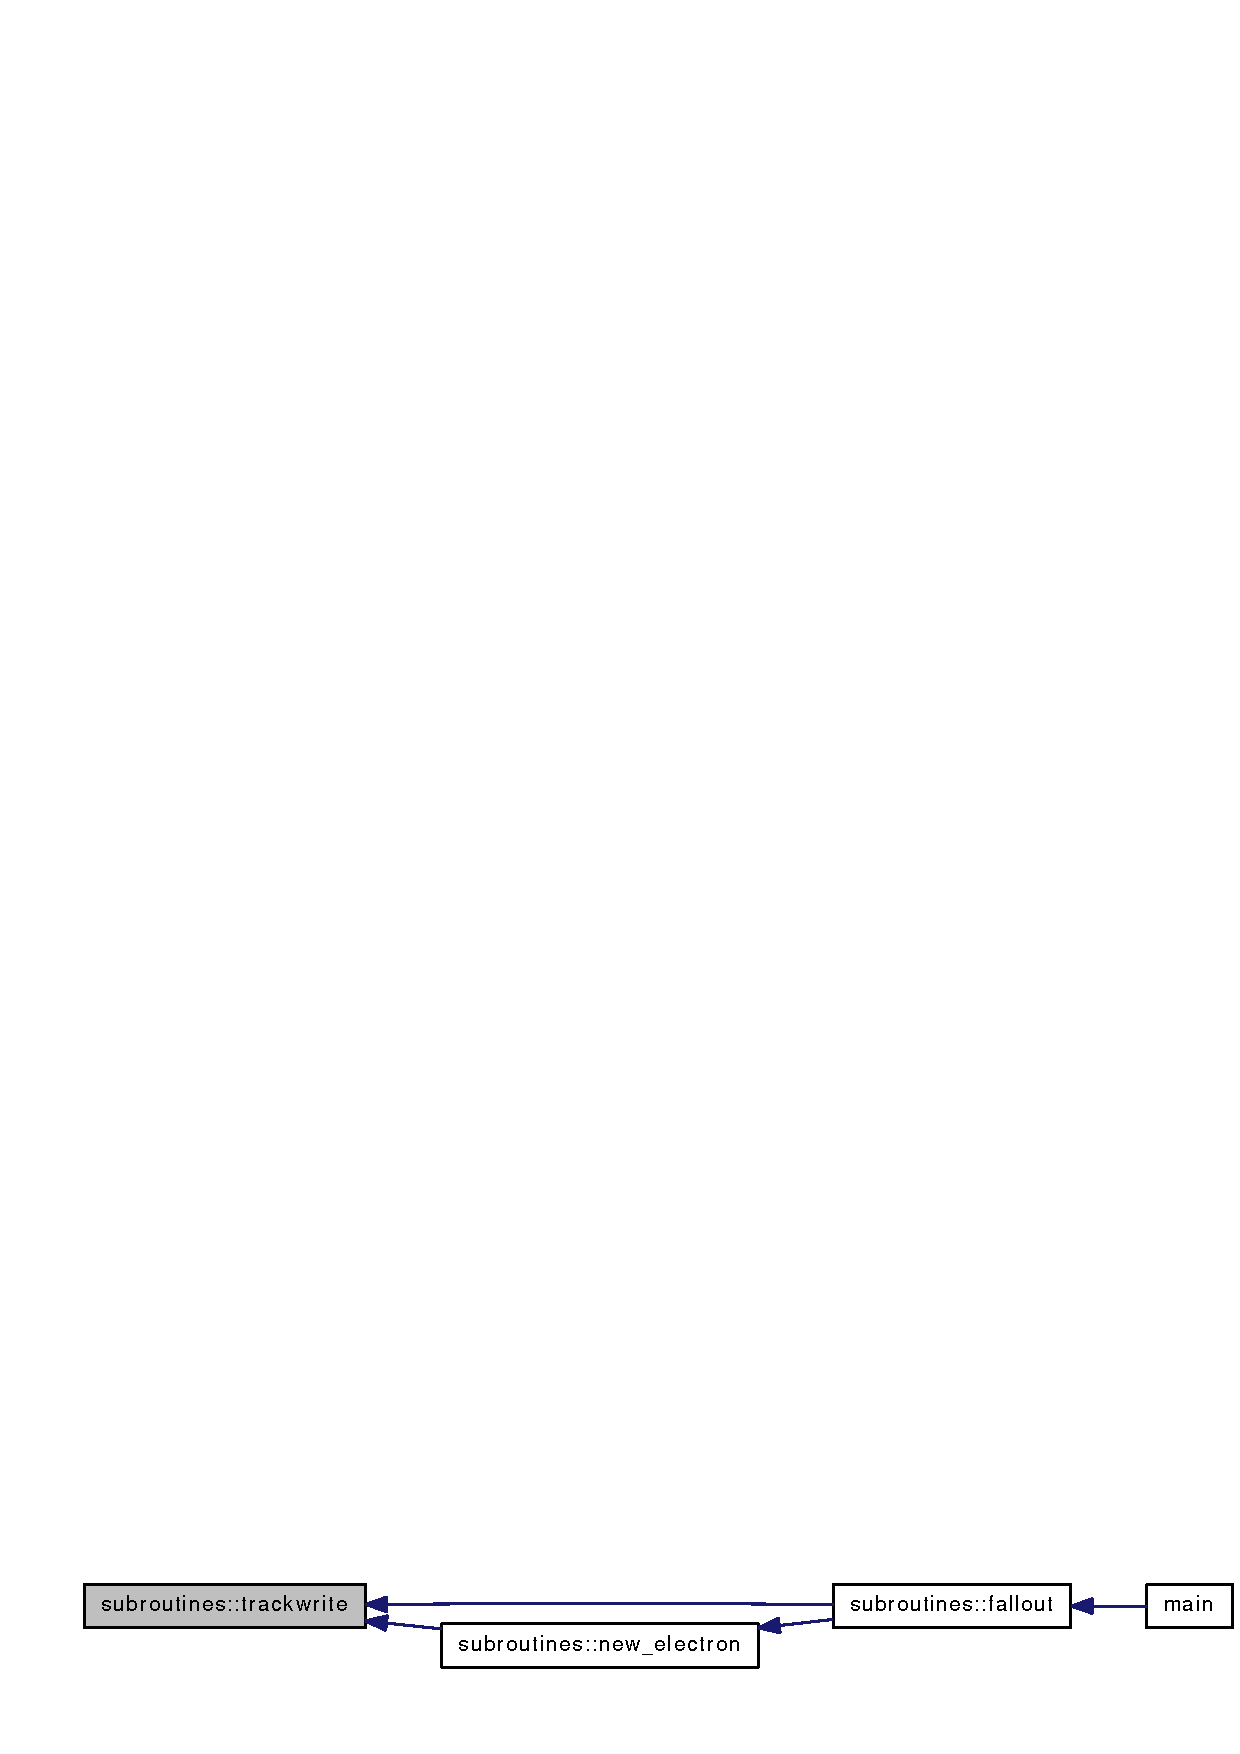
\includegraphics[width=298pt]{namespacesubroutines_abbce0f7ec92c43ac91db25f512531642_icgraph}
\end{center}
\end{figure}
\hypertarget{namespacesubroutines_a0a51843cbd2415487f29e4314e1de97a}{
\index{subroutines@{subroutines}!transport@{transport}}
\index{transport@{transport}!subroutines@{subroutines}}
\subsubsection[{transport}]{\setlength{\rightskip}{0pt plus 5cm}subroutine subroutines::transport (INTEGER,dimension(3),intent(in) {\em prev}, \/  INTEGER,dimension(3),intent(in) {\em curr}, \/  INTEGER,dimension(3),intent(out) {\em next})}}
\label{namespacesubroutines_a0a51843cbd2415487f29e4314e1de97a}


Definition at line 972 of file subroutines.f90.

References parameters::DIMENS, and hopping().

Referenced by find\_\-empty\_\-site(), and new\_\-electron().

Here is the call graph for this function:\nopagebreak
\begin{figure}[H]
\begin{center}
\leavevmode
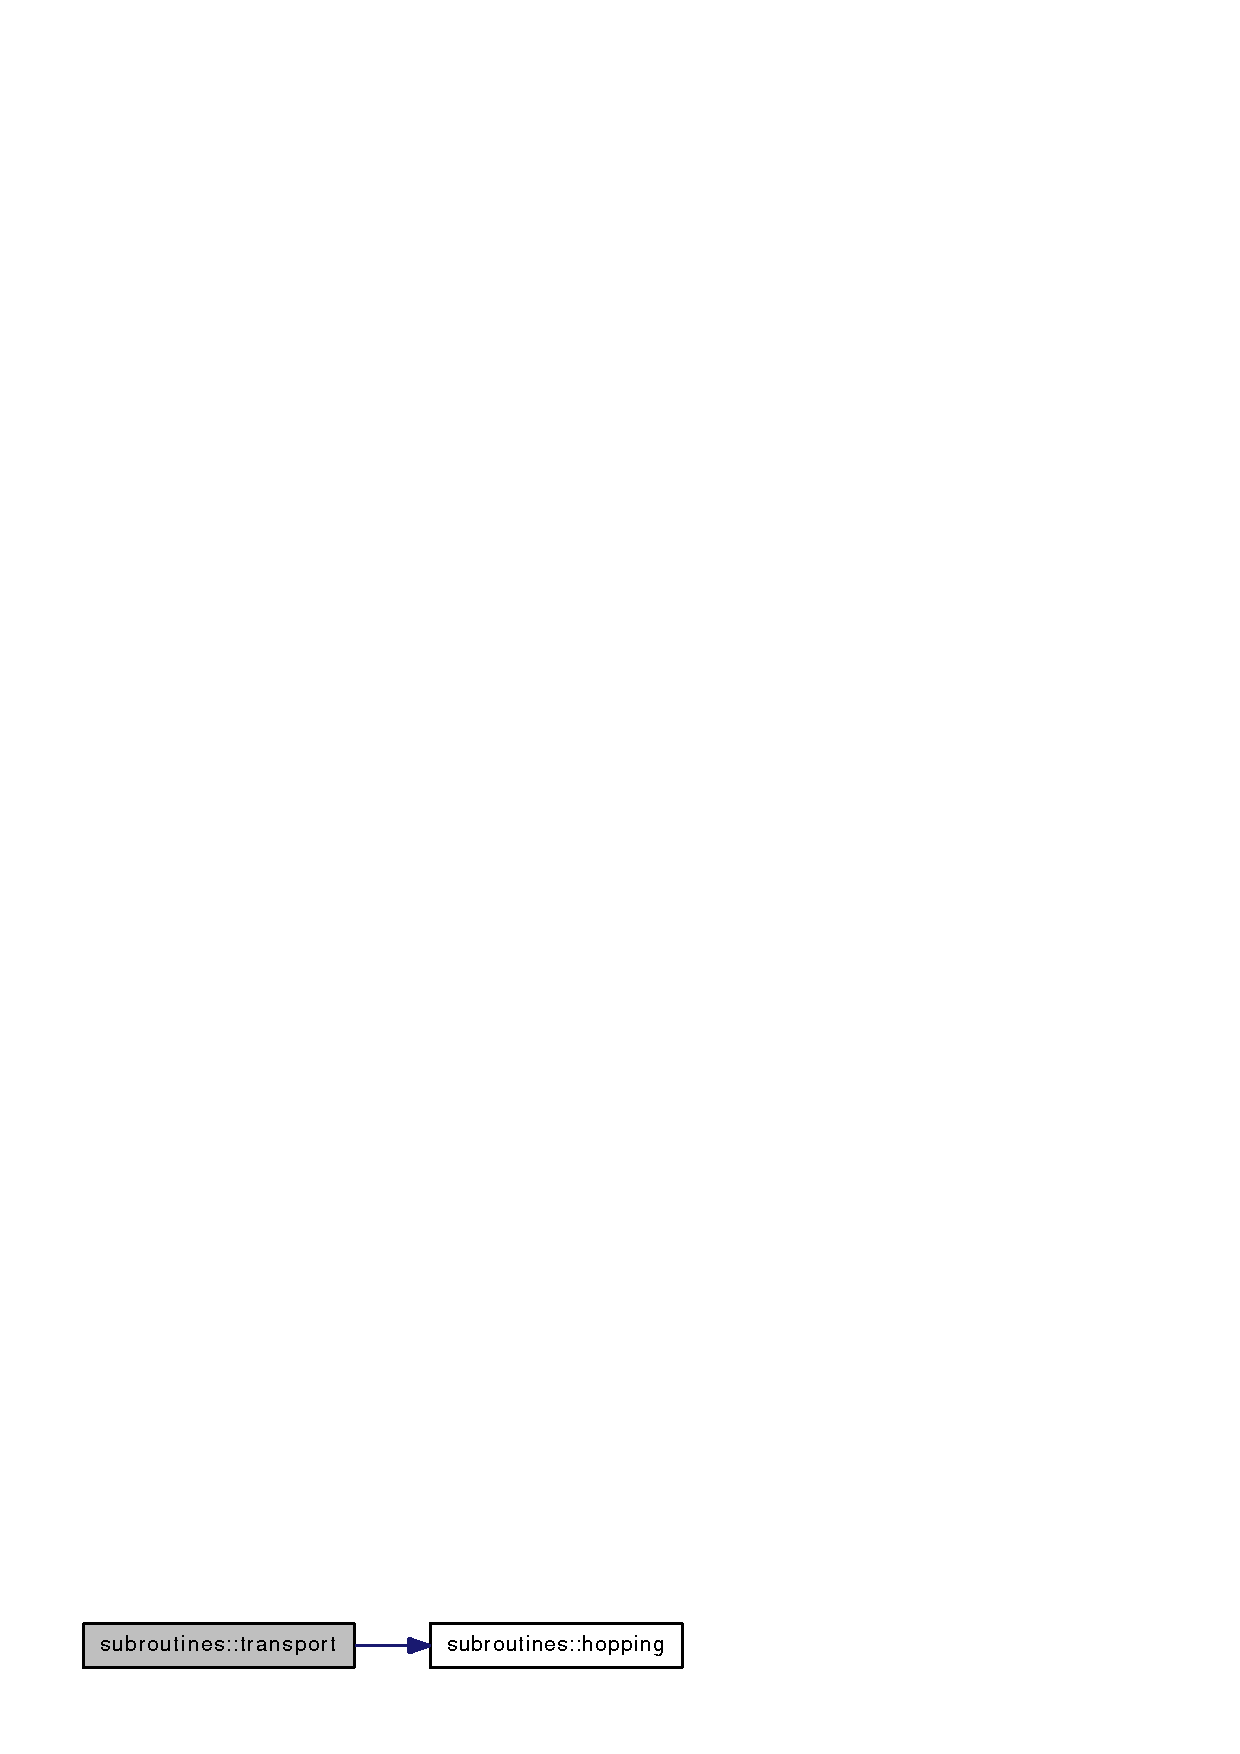
\includegraphics[width=166pt]{namespacesubroutines_a0a51843cbd2415487f29e4314e1de97a_cgraph}
\end{center}
\end{figure}


Here is the caller graph for this function:\nopagebreak
\begin{figure}[H]
\begin{center}
\leavevmode
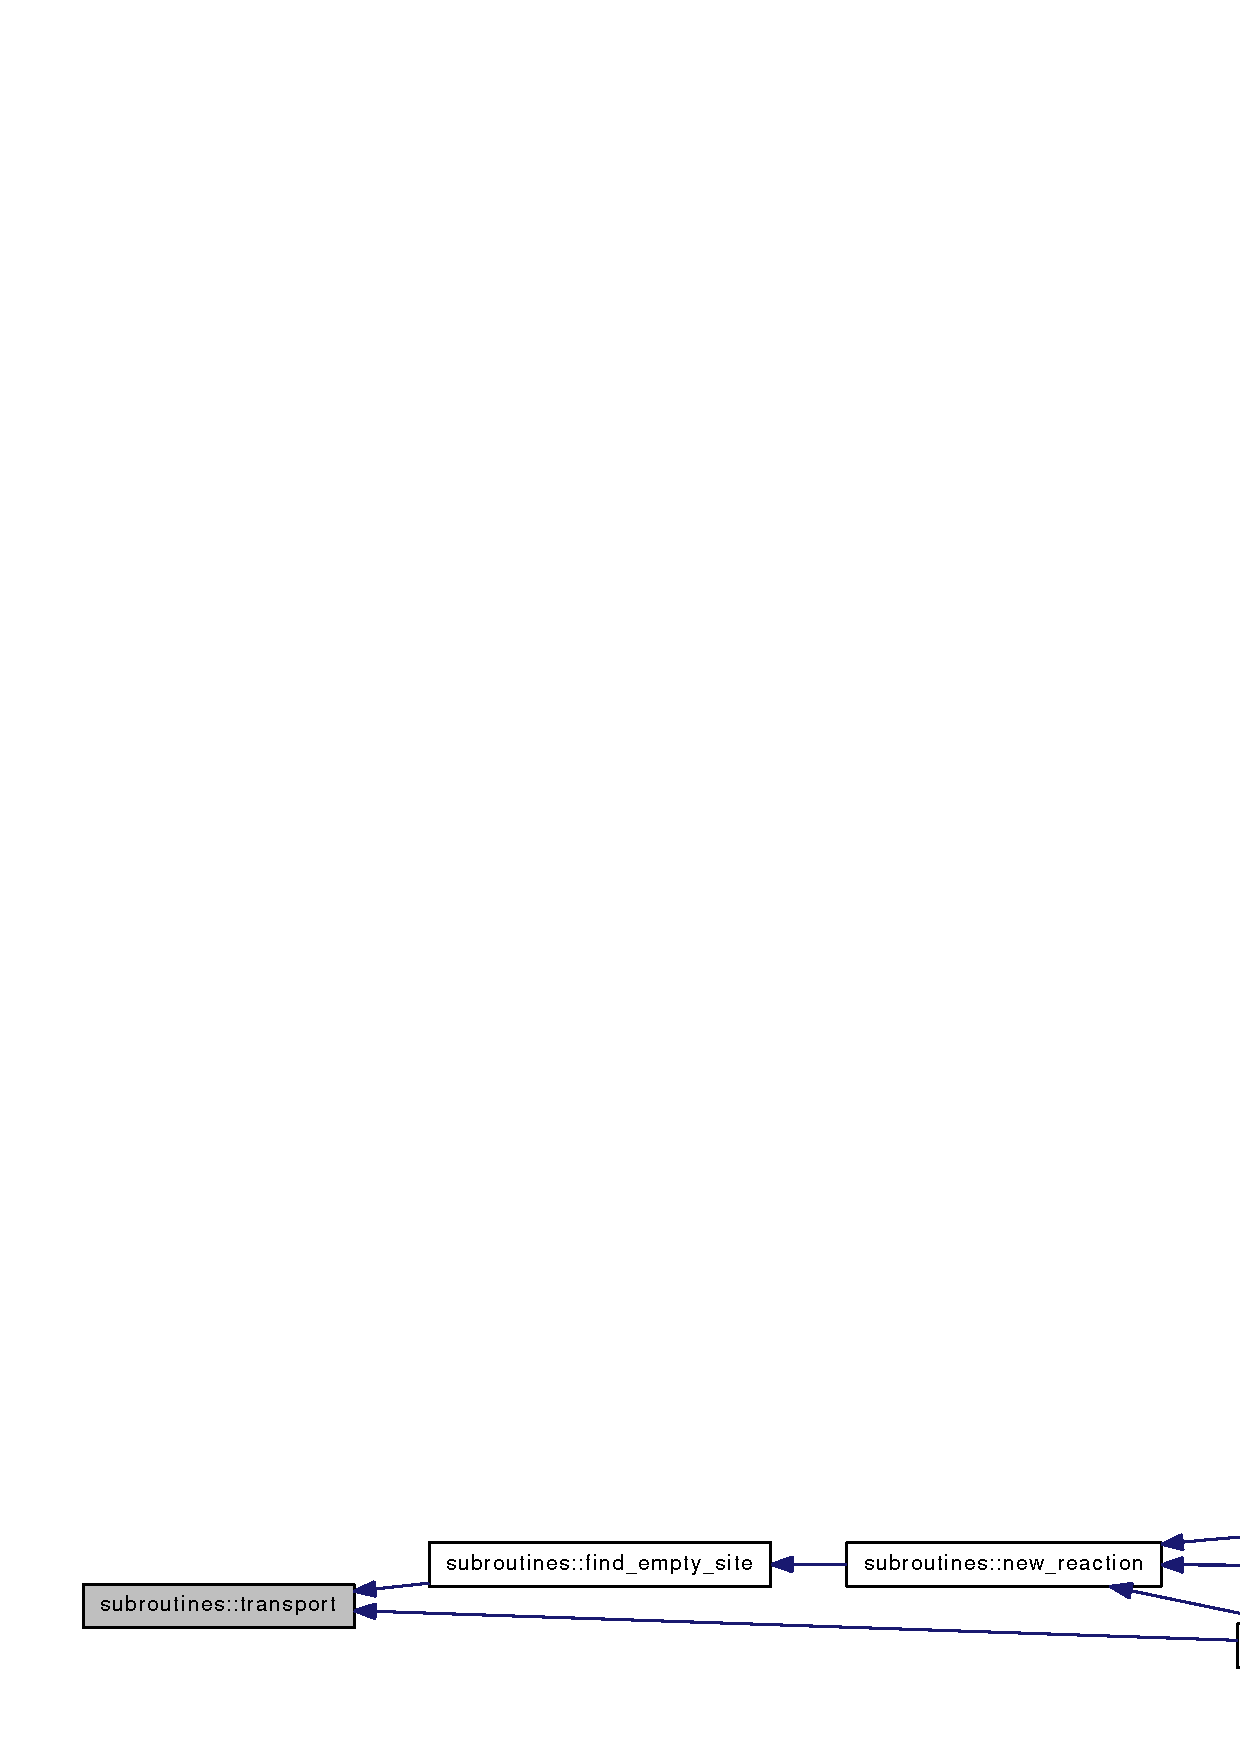
\includegraphics[width=420pt]{namespacesubroutines_a0a51843cbd2415487f29e4314e1de97a_icgraph}
\end{center}
\end{figure}
\hypertarget{namespacesubroutines_ac847bd99eab89bdc881d885b2808624d}{
\index{subroutines@{subroutines}!wait\_\-calc@{wait\_\-calc}}
\index{wait\_\-calc@{wait\_\-calc}!subroutines@{subroutines}}
\subsubsection[{wait\_\-calc}]{\setlength{\rightskip}{0pt plus 5cm}subroutine subroutines::wait\_\-calc (TYPE(node),pointer {\em temp})}}
\label{namespacesubroutines_ac847bd99eab89bdc881d885b2808624d}


Definition at line 754 of file subroutines.f90.

References parameters::DEBUG, parameters::E\_\-BULK, parameters::E\_\-SURF, parameters::EN\_\-LIST, parameters::fast\_\-reacts, hopping(), parameters::MATRIX, parameters::TIME, and parameters::TRL\_\-NU.

Referenced by init\_\-node(), main(), and new\_\-reaction().

Here is the call graph for this function:\nopagebreak
\begin{figure}[H]
\begin{center}
\leavevmode
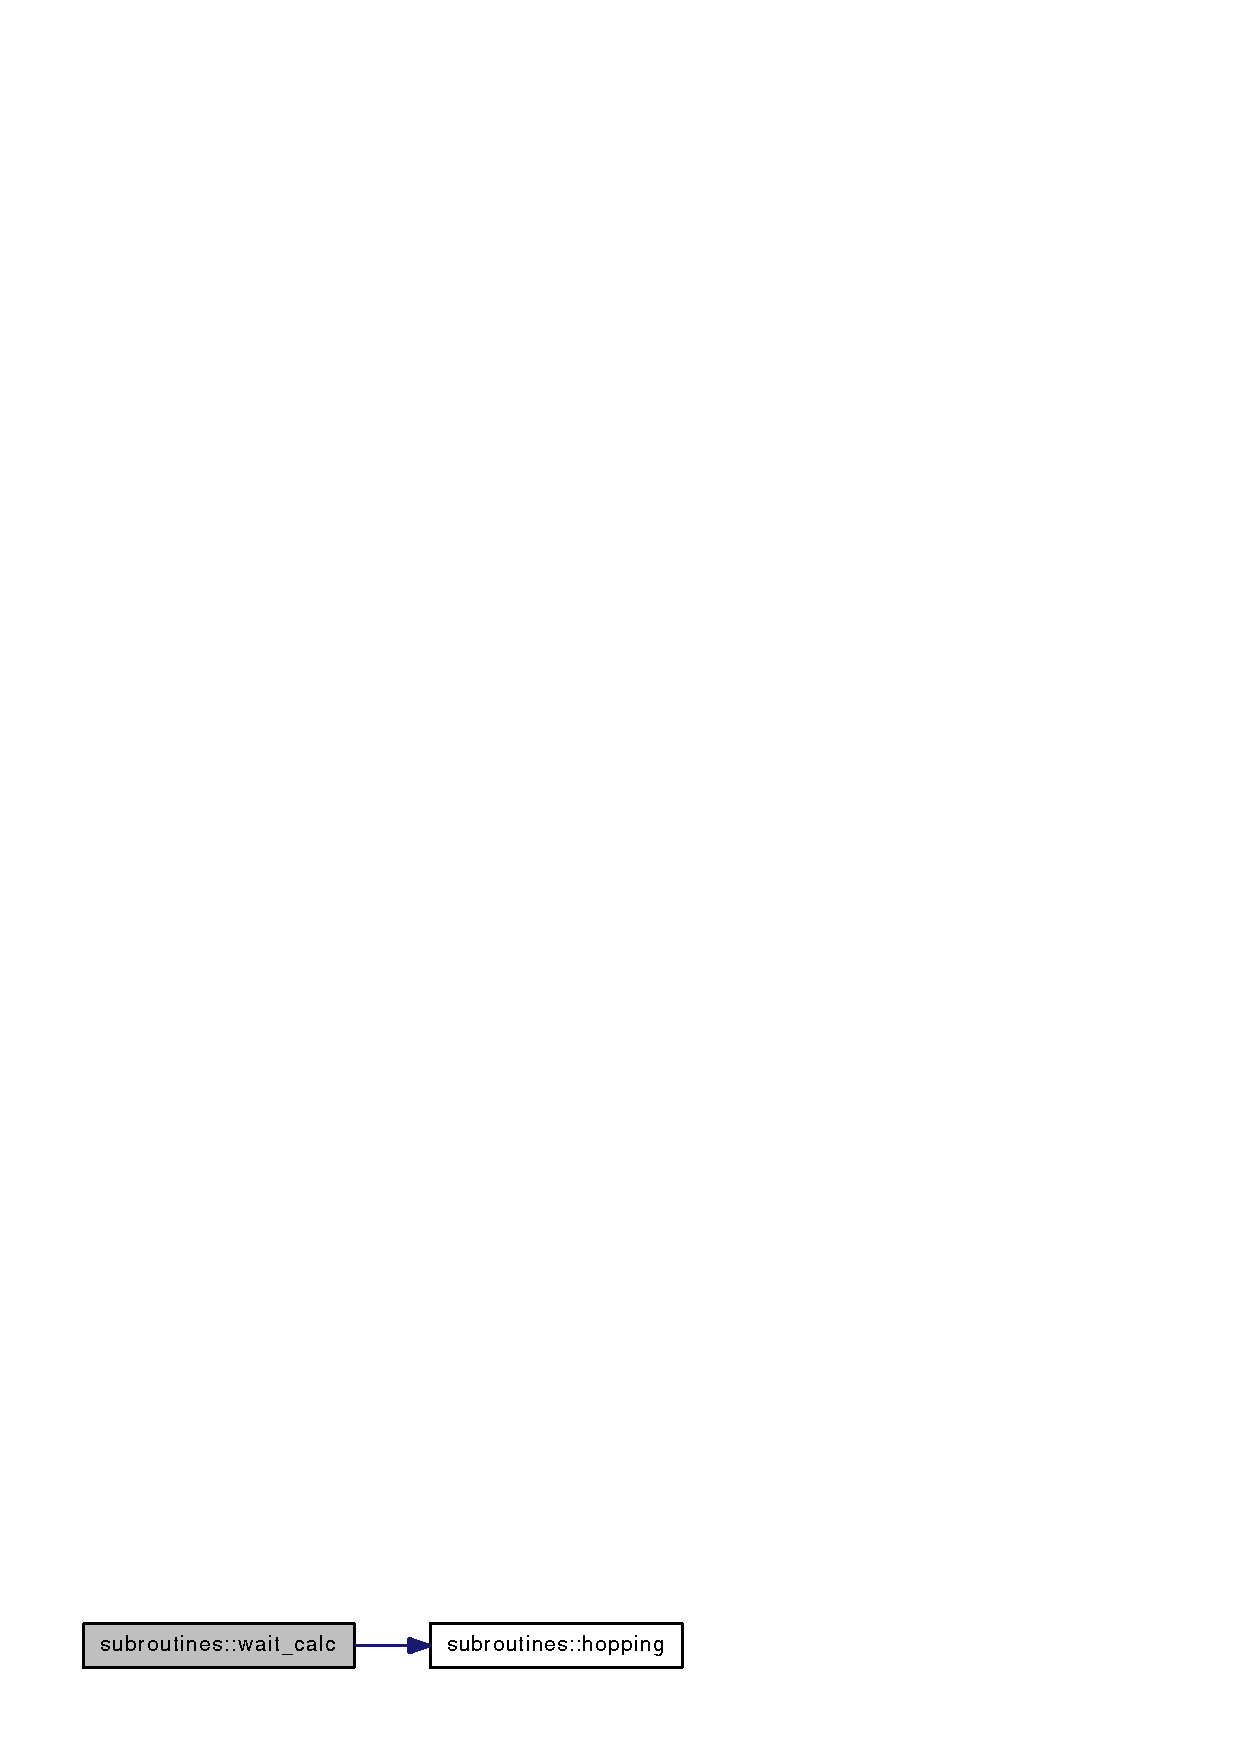
\includegraphics[width=166pt]{namespacesubroutines_ac847bd99eab89bdc881d885b2808624d_cgraph}
\end{center}
\end{figure}


Here is the caller graph for this function:\nopagebreak
\begin{figure}[H]
\begin{center}
\leavevmode
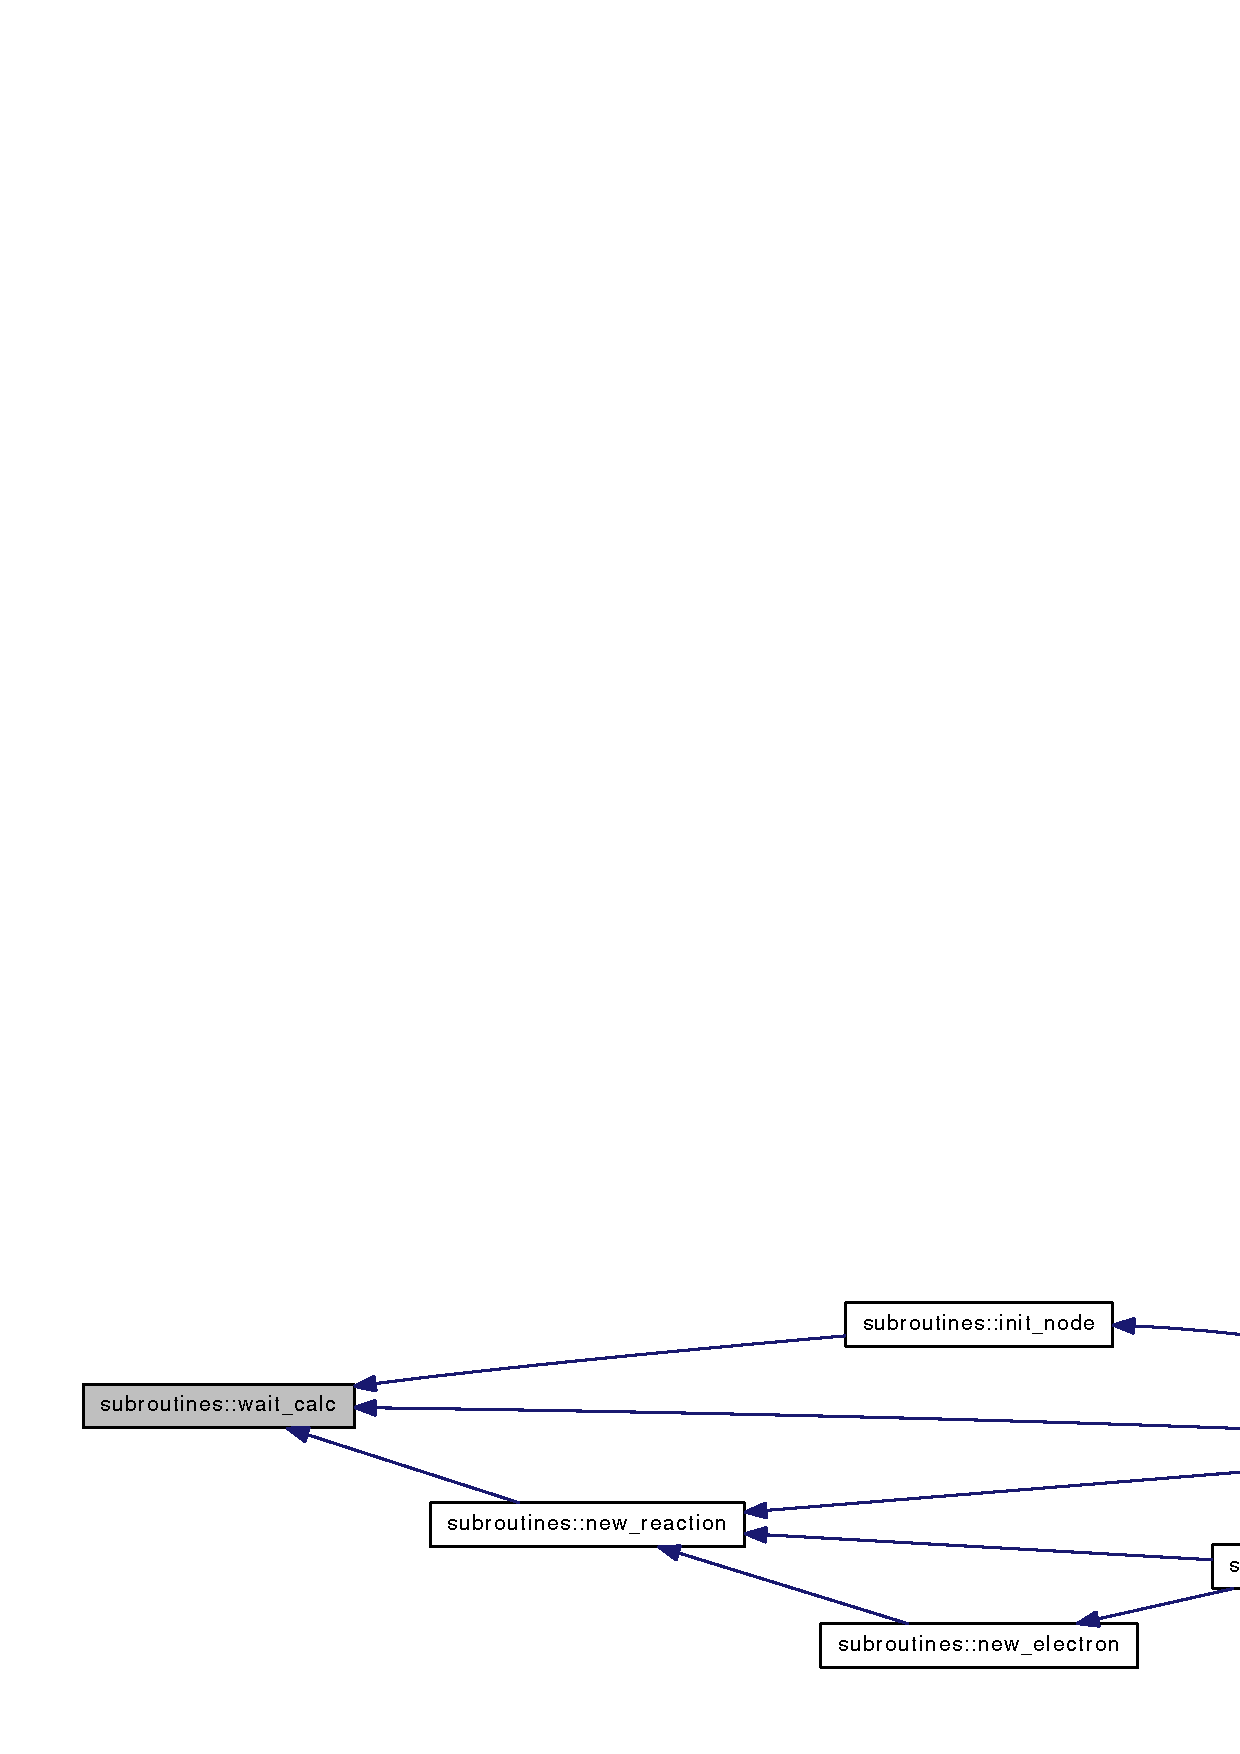
\includegraphics[width=389pt]{namespacesubroutines_ac847bd99eab89bdc881d885b2808624d_icgraph}
\end{center}
\end{figure}
\hypertarget{namespacesubroutines_a7580fc0416f20d44b3cfa79ebc20a839}{
\index{subroutines@{subroutines}!wipe\_\-node@{wipe\_\-node}}
\index{wipe\_\-node@{wipe\_\-node}!subroutines@{subroutines}}
\subsubsection[{wipe\_\-node}]{\setlength{\rightskip}{0pt plus 5cm}subroutine subroutines::wipe\_\-node (INTEGER {\em x}, \/  INTEGER {\em y}, \/  INTEGER {\em z})}}
\label{namespacesubroutines_a7580fc0416f20d44b3cfa79ebc20a839}


Definition at line 2026 of file subroutines.f90.

References parameters::MATRIX.

Referenced by main(), and new\_\-reaction().

Here is the caller graph for this function:\nopagebreak
\begin{figure}[H]
\begin{center}
\leavevmode
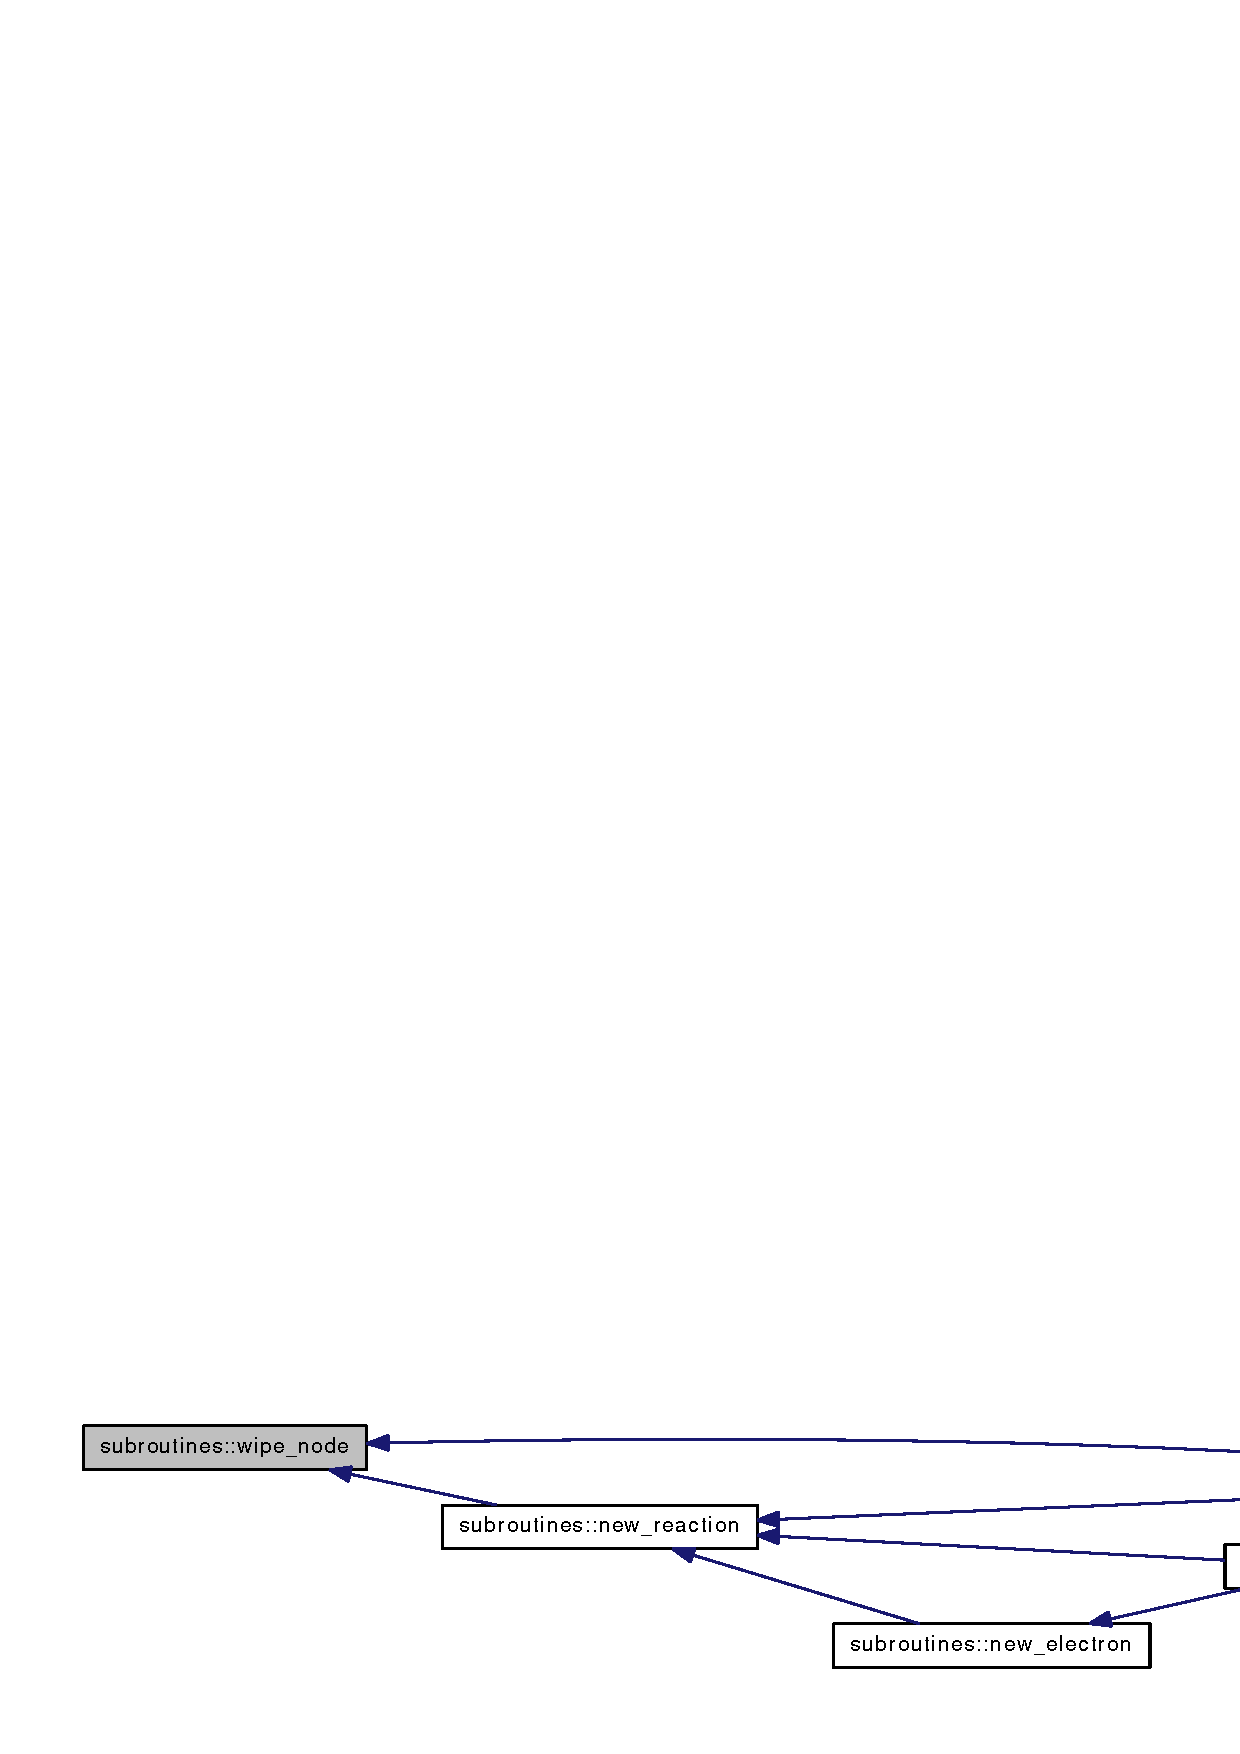
\includegraphics[width=392pt]{namespacesubroutines_a7580fc0416f20d44b3cfa79ebc20a839_icgraph}
\end{center}
\end{figure}
\hypertarget{namespacesubroutines_a0ce9ee9331d3c0bba11e3e00fbd7e07b}{
\index{subroutines@{subroutines}!writereactions@{writereactions}}
\index{writereactions@{writereactions}!subroutines@{subroutines}}
\subsubsection[{writereactions}]{\setlength{\rightskip}{0pt plus 5cm}subroutine subroutines::writereactions (type(reaction) {\em node})}}
\label{namespacesubroutines_a0ce9ee9331d3c0bba11e3e00fbd7e07b}


Definition at line 43 of file subroutines.f90.

References analyzereaction(), parameters::NUM\_\-SPECIES, and parameters::SP\_\-PROD\_\-DEST.

Referenced by counter().

Here is the call graph for this function:\nopagebreak
\begin{figure}[H]
\begin{center}
\leavevmode
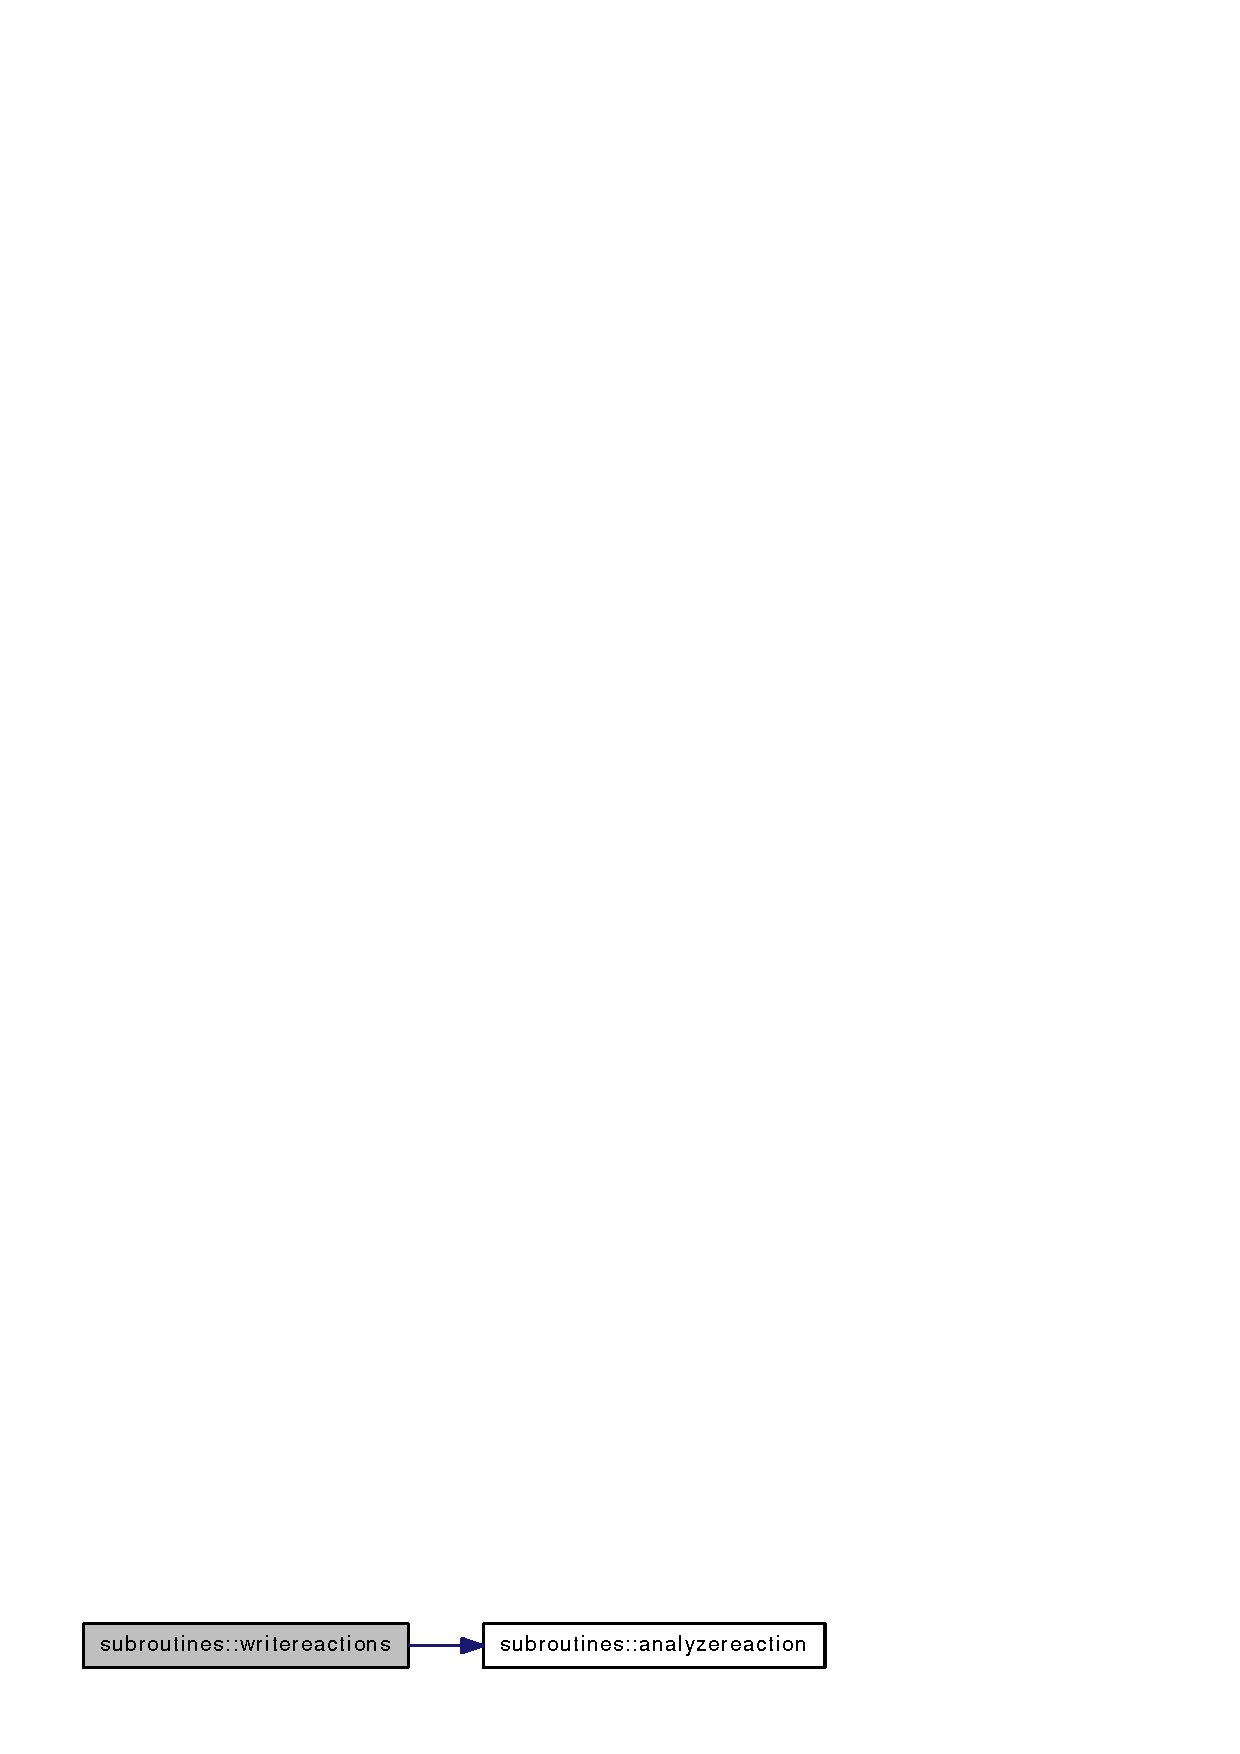
\includegraphics[width=200pt]{namespacesubroutines_a0ce9ee9331d3c0bba11e3e00fbd7e07b_cgraph}
\end{center}
\end{figure}


Here is the caller graph for this function:\nopagebreak
\begin{figure}[H]
\begin{center}
\leavevmode
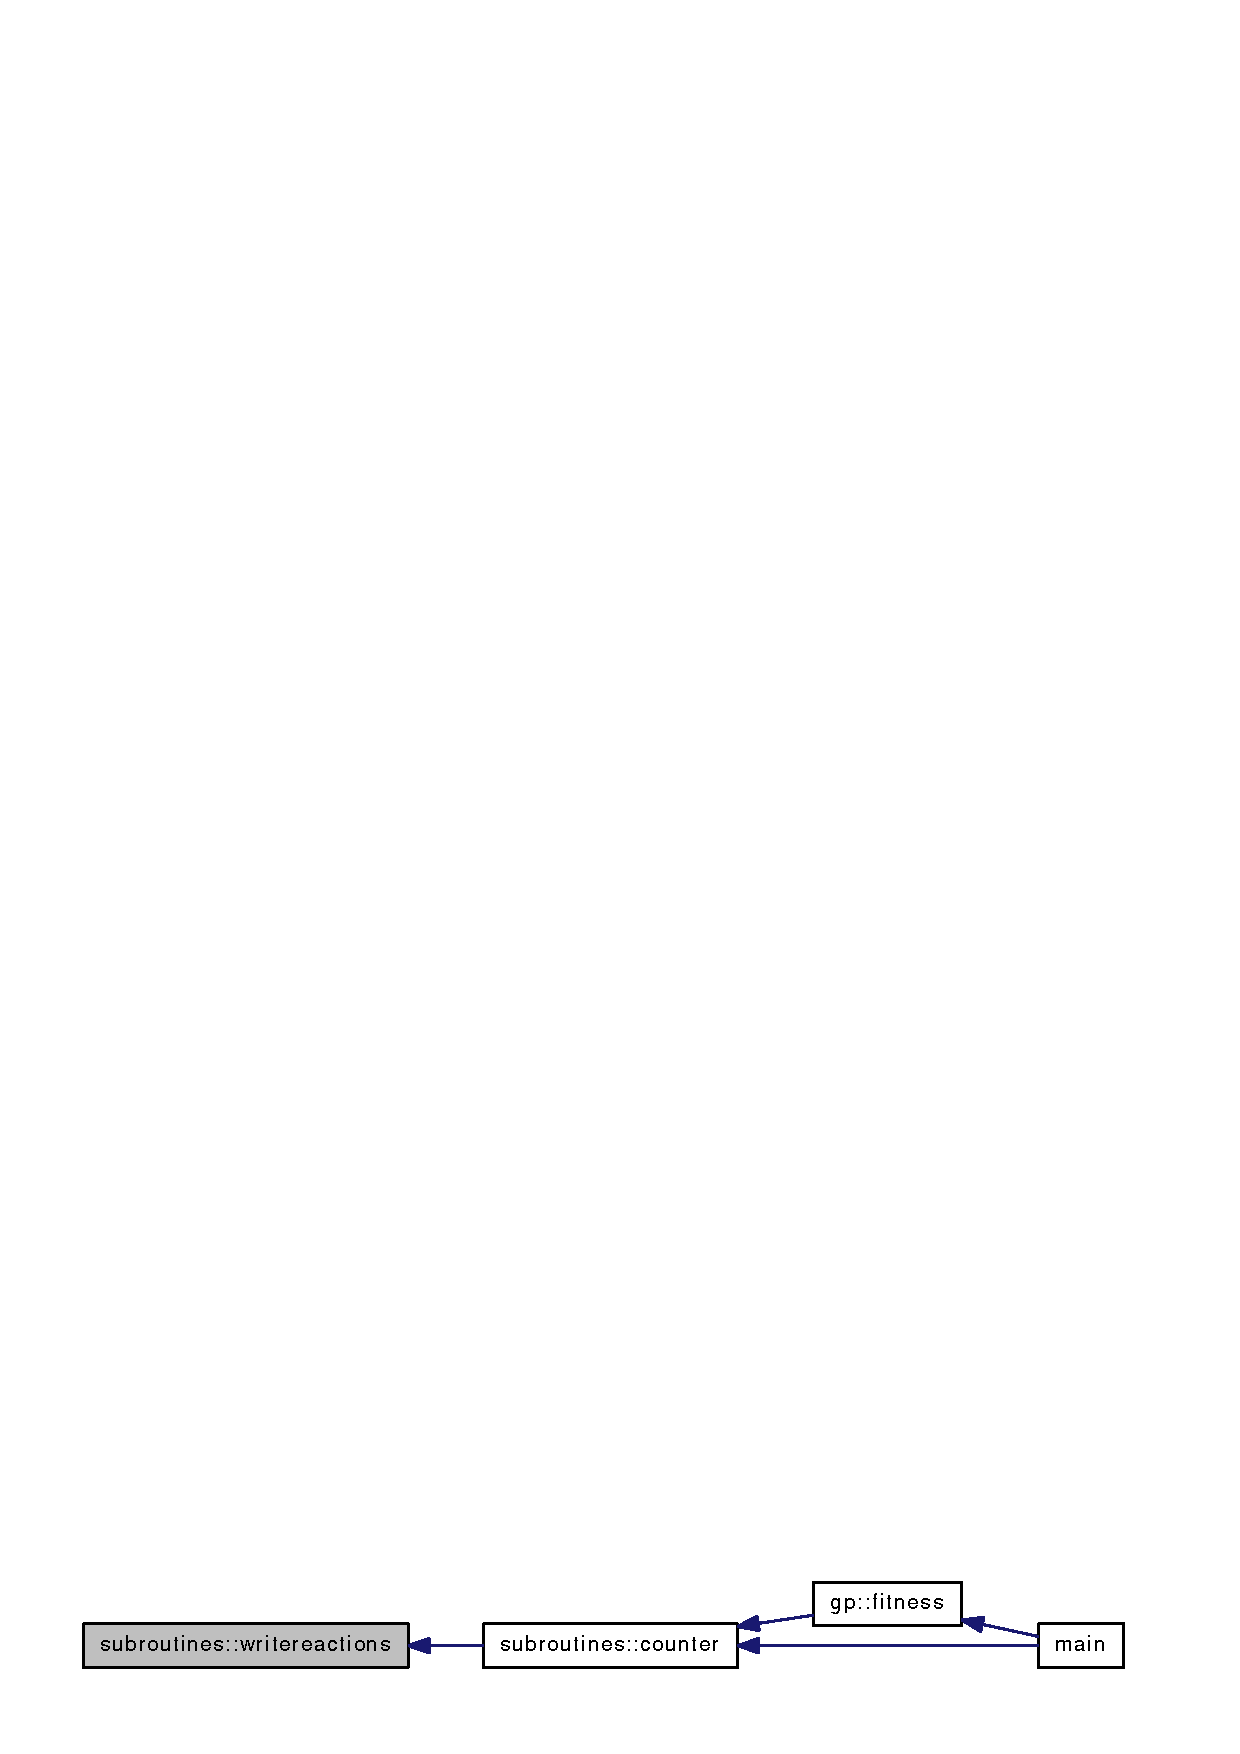
\includegraphics[width=272pt]{namespacesubroutines_a0ce9ee9331d3c0bba11e3e00fbd7e07b_icgraph}
\end{center}
\end{figure}

\hypertarget{namespacetypedefs}{
\section{typedefs Module Reference}
\label{namespacetypedefs}\index{typedefs@{typedefs}}
}
\subsection*{Data Types}
\begin{DoxyCompactItemize}
\item 
type \hyperlink{typetypedefs_1_1wait__info}{wait\_\-info}
\item 
type \hyperlink{typetypedefs_1_1rate__info}{rate\_\-info}
\item 
type \hyperlink{typetypedefs_1_1sigma__box}{sigma\_\-box}
\item 
type \hyperlink{typetypedefs_1_1ionstate}{ionstate}
\item 
type \hyperlink{typetypedefs_1_1alwd__exstate}{alwd\_\-exstate}
\item 
type \hyperlink{typetypedefs_1_1fbdn__exstate}{fbdn\_\-exstate}
\item 
type \hyperlink{typetypedefs_1_1epg__exstate}{epg\_\-exstate}
\item 
type \hyperlink{typetypedefs_1_1epg__ionstate}{epg\_\-ionstate}
\item 
type \hyperlink{typetypedefs_1_1se__info}{se\_\-info}
\item 
type \hyperlink{typetypedefs_1_1node}{node}
\item 
type \hyperlink{typetypedefs_1_1species}{species}
\item 
type \hyperlink{typetypedefs_1_1reaction}{reaction}
\item 
type \hyperlink{typetypedefs_1_1reaction__info}{reaction\_\-info}
\end{DoxyCompactItemize}

\chapter{Data Type Documentation}
\hypertarget{typetypedefs_1_1alwd__exstate}{
\section{typedefs::alwd\_\-exstate Type Reference}
\label{typetypedefs_1_1alwd__exstate}\index{typedefs::alwd\_\-exstate@{typedefs::alwd\_\-exstate}}
}
\subsection*{Public Attributes}
\begin{DoxyCompactItemize}
\item 
CHARACTER(len=20) \hyperlink{typetypedefs_1_1alwd__exstate_a50bb7f5c8fb7c9b0d3163fc8c9d59ffb}{termsym\_\-alwd}
\item 
DOUBLE PRECISION \hyperlink{typetypedefs_1_1alwd__exstate_a9af30d9eafe61b2467f45a93bd9784d4}{wj\_\-alwd}
\item 
DOUBLE PRECISION \hyperlink{typetypedefs_1_1alwd__exstate_af4f9dd8da0478384d513170e6a27ed5f}{fj\_\-alwd}
\item 
DOUBLE PRECISION \hyperlink{typetypedefs_1_1alwd__exstate_ab6b82be801ff29ffee0964542c954f40}{cj\_\-alwd}
\item 
DOUBLE PRECISION \hyperlink{typetypedefs_1_1alwd__exstate_a33893b22b042d2f842d76212b2841830}{alpha\_\-alwd}
\item 
DOUBLE PRECISION \hyperlink{typetypedefs_1_1alwd__exstate_ade69cd51a1551171ecba3fe034aae174}{beta\_\-alwd}
\end{DoxyCompactItemize}


\subsection{Detailed Description}


Definition at line 54 of file typedefs.f90.

\subsection{Member Data Documentation}
\hypertarget{typetypedefs_1_1alwd__exstate_a33893b22b042d2f842d76212b2841830}{
\index{typedefs::alwd\_\-exstate@{typedefs::alwd\_\-exstate}!alpha\_\-alwd@{alpha\_\-alwd}}
\index{alpha\_\-alwd@{alpha\_\-alwd}!typedefs::alwd_exstate@{typedefs::alwd\_\-exstate}}
\subsubsection[{alpha\_\-alwd}]{\setlength{\rightskip}{0pt plus 5cm}DOUBLE PRECISION {\bf typedefs::alwd\_\-exstate::alpha\_\-alwd}}}
\label{typetypedefs_1_1alwd__exstate_a33893b22b042d2f842d76212b2841830}


Definition at line 66 of file typedefs.f90.\hypertarget{typetypedefs_1_1alwd__exstate_ade69cd51a1551171ecba3fe034aae174}{
\index{typedefs::alwd\_\-exstate@{typedefs::alwd\_\-exstate}!beta\_\-alwd@{beta\_\-alwd}}
\index{beta\_\-alwd@{beta\_\-alwd}!typedefs::alwd_exstate@{typedefs::alwd\_\-exstate}}
\subsubsection[{beta\_\-alwd}]{\setlength{\rightskip}{0pt plus 5cm}DOUBLE PRECISION {\bf typedefs::alwd\_\-exstate::beta\_\-alwd}}}
\label{typetypedefs_1_1alwd__exstate_ade69cd51a1551171ecba3fe034aae174}


Definition at line 67 of file typedefs.f90.\hypertarget{typetypedefs_1_1alwd__exstate_ab6b82be801ff29ffee0964542c954f40}{
\index{typedefs::alwd\_\-exstate@{typedefs::alwd\_\-exstate}!cj\_\-alwd@{cj\_\-alwd}}
\index{cj\_\-alwd@{cj\_\-alwd}!typedefs::alwd_exstate@{typedefs::alwd\_\-exstate}}
\subsubsection[{cj\_\-alwd}]{\setlength{\rightskip}{0pt plus 5cm}DOUBLE PRECISION {\bf typedefs::alwd\_\-exstate::cj\_\-alwd}}}
\label{typetypedefs_1_1alwd__exstate_ab6b82be801ff29ffee0964542c954f40}


Definition at line 65 of file typedefs.f90.\hypertarget{typetypedefs_1_1alwd__exstate_af4f9dd8da0478384d513170e6a27ed5f}{
\index{typedefs::alwd\_\-exstate@{typedefs::alwd\_\-exstate}!fj\_\-alwd@{fj\_\-alwd}}
\index{fj\_\-alwd@{fj\_\-alwd}!typedefs::alwd_exstate@{typedefs::alwd\_\-exstate}}
\subsubsection[{fj\_\-alwd}]{\setlength{\rightskip}{0pt plus 5cm}DOUBLE PRECISION {\bf typedefs::alwd\_\-exstate::fj\_\-alwd}}}
\label{typetypedefs_1_1alwd__exstate_af4f9dd8da0478384d513170e6a27ed5f}


Definition at line 64 of file typedefs.f90.\hypertarget{typetypedefs_1_1alwd__exstate_a50bb7f5c8fb7c9b0d3163fc8c9d59ffb}{
\index{typedefs::alwd\_\-exstate@{typedefs::alwd\_\-exstate}!termsym\_\-alwd@{termsym\_\-alwd}}
\index{termsym\_\-alwd@{termsym\_\-alwd}!typedefs::alwd_exstate@{typedefs::alwd\_\-exstate}}
\subsubsection[{termsym\_\-alwd}]{\setlength{\rightskip}{0pt plus 5cm}CHARACTER(len=20) {\bf typedefs::alwd\_\-exstate::termsym\_\-alwd}}}
\label{typetypedefs_1_1alwd__exstate_a50bb7f5c8fb7c9b0d3163fc8c9d59ffb}


Definition at line 62 of file typedefs.f90.\hypertarget{typetypedefs_1_1alwd__exstate_a9af30d9eafe61b2467f45a93bd9784d4}{
\index{typedefs::alwd\_\-exstate@{typedefs::alwd\_\-exstate}!wj\_\-alwd@{wj\_\-alwd}}
\index{wj\_\-alwd@{wj\_\-alwd}!typedefs::alwd_exstate@{typedefs::alwd\_\-exstate}}
\subsubsection[{wj\_\-alwd}]{\setlength{\rightskip}{0pt plus 5cm}DOUBLE PRECISION {\bf typedefs::alwd\_\-exstate::wj\_\-alwd}}}
\label{typetypedefs_1_1alwd__exstate_a9af30d9eafe61b2467f45a93bd9784d4}


Definition at line 63 of file typedefs.f90.

The documentation for this type was generated from the following file:\begin{DoxyCompactItemize}
\item 
\hyperlink{typedefs_8f90}{typedefs.f90}\end{DoxyCompactItemize}

\hypertarget{typetypedefs_1_1epg__exstate}{
\section{typedefs::epg\_\-exstate Type Reference}
\label{typetypedefs_1_1epg__exstate}\index{typedefs::epg\_\-exstate@{typedefs::epg\_\-exstate}}
}
\subsection*{Public Attributes}
\begin{DoxyCompactItemize}
\item 
CHARACTER(len=20) \hyperlink{typetypedefs_1_1epg__exstate_abb12fa8ac79b7b77d90f7dd1f0519222}{termsym\_\-epgex}
\item 
DOUBLE PRECISION \hyperlink{typetypedefs_1_1epg__exstate_a80825059cab2f5a2a47f9233ee2694c3}{a\_\-epgex}
\item 
DOUBLE PRECISION \hyperlink{typetypedefs_1_1epg__exstate_ab752c0ea7171e84c8846f5b45373321c}{j\_\-epgex}
\item 
DOUBLE PRECISION \hyperlink{typetypedefs_1_1epg__exstate_a10f13ccae9fbfd2620616a1d6f7d7d46}{nu\_\-epgex}
\item 
DOUBLE PRECISION \hyperlink{typetypedefs_1_1epg__exstate_a46024cb2b6ef6bd809a2ee3d43769b60}{omega\_\-epgex}
\item 
DOUBLE PRECISION \hyperlink{typetypedefs_1_1epg__exstate_a06dc6c0176150e54c25ebc5de0f9a50c}{w\_\-epgex}
\end{DoxyCompactItemize}


\subsection{Detailed Description}


Definition at line 83 of file typedefs.f90.

\subsection{Member Data Documentation}
\hypertarget{typetypedefs_1_1epg__exstate_a80825059cab2f5a2a47f9233ee2694c3}{
\index{typedefs::epg\_\-exstate@{typedefs::epg\_\-exstate}!a\_\-epgex@{a\_\-epgex}}
\index{a\_\-epgex@{a\_\-epgex}!typedefs::epg_exstate@{typedefs::epg\_\-exstate}}
\subsubsection[{a\_\-epgex}]{\setlength{\rightskip}{0pt plus 5cm}DOUBLE PRECISION {\bf typedefs::epg\_\-exstate::a\_\-epgex}}}
\label{typetypedefs_1_1epg__exstate_a80825059cab2f5a2a47f9233ee2694c3}


Definition at line 89 of file typedefs.f90.\hypertarget{typetypedefs_1_1epg__exstate_ab752c0ea7171e84c8846f5b45373321c}{
\index{typedefs::epg\_\-exstate@{typedefs::epg\_\-exstate}!j\_\-epgex@{j\_\-epgex}}
\index{j\_\-epgex@{j\_\-epgex}!typedefs::epg_exstate@{typedefs::epg\_\-exstate}}
\subsubsection[{j\_\-epgex}]{\setlength{\rightskip}{0pt plus 5cm}DOUBLE PRECISION {\bf typedefs::epg\_\-exstate::j\_\-epgex}}}
\label{typetypedefs_1_1epg__exstate_ab752c0ea7171e84c8846f5b45373321c}


Definition at line 90 of file typedefs.f90.\hypertarget{typetypedefs_1_1epg__exstate_a10f13ccae9fbfd2620616a1d6f7d7d46}{
\index{typedefs::epg\_\-exstate@{typedefs::epg\_\-exstate}!nu\_\-epgex@{nu\_\-epgex}}
\index{nu\_\-epgex@{nu\_\-epgex}!typedefs::epg_exstate@{typedefs::epg\_\-exstate}}
\subsubsection[{nu\_\-epgex}]{\setlength{\rightskip}{0pt plus 5cm}DOUBLE PRECISION {\bf typedefs::epg\_\-exstate::nu\_\-epgex}}}
\label{typetypedefs_1_1epg__exstate_a10f13ccae9fbfd2620616a1d6f7d7d46}


Definition at line 91 of file typedefs.f90.\hypertarget{typetypedefs_1_1epg__exstate_a46024cb2b6ef6bd809a2ee3d43769b60}{
\index{typedefs::epg\_\-exstate@{typedefs::epg\_\-exstate}!omega\_\-epgex@{omega\_\-epgex}}
\index{omega\_\-epgex@{omega\_\-epgex}!typedefs::epg_exstate@{typedefs::epg\_\-exstate}}
\subsubsection[{omega\_\-epgex}]{\setlength{\rightskip}{0pt plus 5cm}DOUBLE PRECISION {\bf typedefs::epg\_\-exstate::omega\_\-epgex}}}
\label{typetypedefs_1_1epg__exstate_a46024cb2b6ef6bd809a2ee3d43769b60}


Definition at line 92 of file typedefs.f90.\hypertarget{typetypedefs_1_1epg__exstate_abb12fa8ac79b7b77d90f7dd1f0519222}{
\index{typedefs::epg\_\-exstate@{typedefs::epg\_\-exstate}!termsym\_\-epgex@{termsym\_\-epgex}}
\index{termsym\_\-epgex@{termsym\_\-epgex}!typedefs::epg_exstate@{typedefs::epg\_\-exstate}}
\subsubsection[{termsym\_\-epgex}]{\setlength{\rightskip}{0pt plus 5cm}CHARACTER(len=20) {\bf typedefs::epg\_\-exstate::termsym\_\-epgex}}}
\label{typetypedefs_1_1epg__exstate_abb12fa8ac79b7b77d90f7dd1f0519222}


Definition at line 88 of file typedefs.f90.\hypertarget{typetypedefs_1_1epg__exstate_a06dc6c0176150e54c25ebc5de0f9a50c}{
\index{typedefs::epg\_\-exstate@{typedefs::epg\_\-exstate}!w\_\-epgex@{w\_\-epgex}}
\index{w\_\-epgex@{w\_\-epgex}!typedefs::epg_exstate@{typedefs::epg\_\-exstate}}
\subsubsection[{w\_\-epgex}]{\setlength{\rightskip}{0pt plus 5cm}DOUBLE PRECISION {\bf typedefs::epg\_\-exstate::w\_\-epgex}}}
\label{typetypedefs_1_1epg__exstate_a06dc6c0176150e54c25ebc5de0f9a50c}


Definition at line 93 of file typedefs.f90.

The documentation for this type was generated from the following file:\begin{DoxyCompactItemize}
\item 
\hyperlink{typedefs_8f90}{typedefs.f90}\end{DoxyCompactItemize}

\hypertarget{typetypedefs_1_1epg__ionstate}{
\section{typedefs::epg\_\-ionstate Type Reference}
\label{typetypedefs_1_1epg__ionstate}\index{typedefs::epg\_\-ionstate@{typedefs::epg\_\-ionstate}}
}
\subsection*{Public Attributes}
\begin{DoxyCompactItemize}
\item 
CHARACTER(len=20) \hyperlink{typetypedefs_1_1epg__ionstate_ab4319012611e6467da11e7c374dda89c}{termsym\_\-epgion}
\item 
DOUBLE PRECISION \hyperlink{typetypedefs_1_1epg__ionstate_a26ebf9bef52002dee95c0cd61f39c784}{a\_\-epgion}
\item 
DOUBLE PRECISION \hyperlink{typetypedefs_1_1epg__ionstate_af58a6a50862ca7fa102f7cfb4fbfa048}{j\_\-epgion}
\item 
DOUBLE PRECISION \hyperlink{typetypedefs_1_1epg__ionstate_a223a1bee73dd96f76979196b8eced4ff}{nu\_\-epgion}
\item 
DOUBLE PRECISION \hyperlink{typetypedefs_1_1epg__ionstate_a83358e3fa4910f5d22f255d17ac27210}{omega\_\-epgion}
\item 
DOUBLE PRECISION \hyperlink{typetypedefs_1_1epg__ionstate_a6a8f71bd76a8bc224110dddd0879e737}{i\_\-epgion}
\end{DoxyCompactItemize}


\subsection{Detailed Description}


Definition at line 96 of file typedefs.f90.

\subsection{Member Data Documentation}
\hypertarget{typetypedefs_1_1epg__ionstate_a26ebf9bef52002dee95c0cd61f39c784}{
\index{typedefs::epg\_\-ionstate@{typedefs::epg\_\-ionstate}!a\_\-epgion@{a\_\-epgion}}
\index{a\_\-epgion@{a\_\-epgion}!typedefs::epg_ionstate@{typedefs::epg\_\-ionstate}}
\subsubsection[{a\_\-epgion}]{\setlength{\rightskip}{0pt plus 5cm}DOUBLE PRECISION {\bf typedefs::epg\_\-ionstate::a\_\-epgion}}}
\label{typetypedefs_1_1epg__ionstate_a26ebf9bef52002dee95c0cd61f39c784}


Definition at line 101 of file typedefs.f90.\hypertarget{typetypedefs_1_1epg__ionstate_a6a8f71bd76a8bc224110dddd0879e737}{
\index{typedefs::epg\_\-ionstate@{typedefs::epg\_\-ionstate}!i\_\-epgion@{i\_\-epgion}}
\index{i\_\-epgion@{i\_\-epgion}!typedefs::epg_ionstate@{typedefs::epg\_\-ionstate}}
\subsubsection[{i\_\-epgion}]{\setlength{\rightskip}{0pt plus 5cm}DOUBLE PRECISION {\bf typedefs::epg\_\-ionstate::i\_\-epgion}}}
\label{typetypedefs_1_1epg__ionstate_a6a8f71bd76a8bc224110dddd0879e737}


Definition at line 105 of file typedefs.f90.\hypertarget{typetypedefs_1_1epg__ionstate_af58a6a50862ca7fa102f7cfb4fbfa048}{
\index{typedefs::epg\_\-ionstate@{typedefs::epg\_\-ionstate}!j\_\-epgion@{j\_\-epgion}}
\index{j\_\-epgion@{j\_\-epgion}!typedefs::epg_ionstate@{typedefs::epg\_\-ionstate}}
\subsubsection[{j\_\-epgion}]{\setlength{\rightskip}{0pt plus 5cm}DOUBLE PRECISION {\bf typedefs::epg\_\-ionstate::j\_\-epgion}}}
\label{typetypedefs_1_1epg__ionstate_af58a6a50862ca7fa102f7cfb4fbfa048}


Definition at line 102 of file typedefs.f90.\hypertarget{typetypedefs_1_1epg__ionstate_a223a1bee73dd96f76979196b8eced4ff}{
\index{typedefs::epg\_\-ionstate@{typedefs::epg\_\-ionstate}!nu\_\-epgion@{nu\_\-epgion}}
\index{nu\_\-epgion@{nu\_\-epgion}!typedefs::epg_ionstate@{typedefs::epg\_\-ionstate}}
\subsubsection[{nu\_\-epgion}]{\setlength{\rightskip}{0pt plus 5cm}DOUBLE PRECISION {\bf typedefs::epg\_\-ionstate::nu\_\-epgion}}}
\label{typetypedefs_1_1epg__ionstate_a223a1bee73dd96f76979196b8eced4ff}


Definition at line 103 of file typedefs.f90.\hypertarget{typetypedefs_1_1epg__ionstate_a83358e3fa4910f5d22f255d17ac27210}{
\index{typedefs::epg\_\-ionstate@{typedefs::epg\_\-ionstate}!omega\_\-epgion@{omega\_\-epgion}}
\index{omega\_\-epgion@{omega\_\-epgion}!typedefs::epg_ionstate@{typedefs::epg\_\-ionstate}}
\subsubsection[{omega\_\-epgion}]{\setlength{\rightskip}{0pt plus 5cm}DOUBLE PRECISION {\bf typedefs::epg\_\-ionstate::omega\_\-epgion}}}
\label{typetypedefs_1_1epg__ionstate_a83358e3fa4910f5d22f255d17ac27210}


Definition at line 104 of file typedefs.f90.\hypertarget{typetypedefs_1_1epg__ionstate_ab4319012611e6467da11e7c374dda89c}{
\index{typedefs::epg\_\-ionstate@{typedefs::epg\_\-ionstate}!termsym\_\-epgion@{termsym\_\-epgion}}
\index{termsym\_\-epgion@{termsym\_\-epgion}!typedefs::epg_ionstate@{typedefs::epg\_\-ionstate}}
\subsubsection[{termsym\_\-epgion}]{\setlength{\rightskip}{0pt plus 5cm}CHARACTER(len=20) {\bf typedefs::epg\_\-ionstate::termsym\_\-epgion}}}
\label{typetypedefs_1_1epg__ionstate_ab4319012611e6467da11e7c374dda89c}


Definition at line 100 of file typedefs.f90.

The documentation for this type was generated from the following file:\begin{DoxyCompactItemize}
\item 
\hyperlink{typedefs_8f90}{typedefs.f90}\end{DoxyCompactItemize}

\hypertarget{typetypedefs_1_1fbdn__exstate}{
\section{typedefs::fbdn\_\-exstate Type Reference}
\label{typetypedefs_1_1fbdn__exstate}\index{typedefs::fbdn\_\-exstate@{typedefs::fbdn\_\-exstate}}
}
\subsection*{Public Attributes}
\begin{DoxyCompactItemize}
\item 
CHARACTER(len=20) \hyperlink{typetypedefs_1_1fbdn__exstate_a5d5aa9abbdf8366cd5bd2a88cb2d2cd2}{termsym\_\-fbdn}
\item 
DOUBLE PRECISION \hyperlink{typetypedefs_1_1fbdn__exstate_aaf62d1b6e41c831990923a8e0ca14373}{wj\_\-fbdn}
\item 
DOUBLE PRECISION \hyperlink{typetypedefs_1_1fbdn__exstate_a0acc4647581eff1d24ce1d71d3f73f8b}{fj\_\-fbdn}
\item 
DOUBLE PRECISION \hyperlink{typetypedefs_1_1fbdn__exstate_af1c6388e1f1f6455d2ee128b875f7adc}{omega\_\-fbdn}
\item 
DOUBLE PRECISION \hyperlink{typetypedefs_1_1fbdn__exstate_a2b6818045634ea0071217f07d9985e31}{alpha\_\-fbdn}
\item 
DOUBLE PRECISION \hyperlink{typetypedefs_1_1fbdn__exstate_a690aa05deb0d2ffba11f3ae2aaf0e9af}{beta\_\-fbdn}
\end{DoxyCompactItemize}


\subsection{Detailed Description}


Definition at line 70 of file typedefs.f90.

\subsection{Member Data Documentation}
\hypertarget{typetypedefs_1_1fbdn__exstate_a2b6818045634ea0071217f07d9985e31}{
\index{typedefs::fbdn\_\-exstate@{typedefs::fbdn\_\-exstate}!alpha\_\-fbdn@{alpha\_\-fbdn}}
\index{alpha\_\-fbdn@{alpha\_\-fbdn}!typedefs::fbdn_exstate@{typedefs::fbdn\_\-exstate}}
\subsubsection[{alpha\_\-fbdn}]{\setlength{\rightskip}{0pt plus 5cm}DOUBLE PRECISION {\bf typedefs::fbdn\_\-exstate::alpha\_\-fbdn}}}
\label{typetypedefs_1_1fbdn__exstate_a2b6818045634ea0071217f07d9985e31}


Definition at line 79 of file typedefs.f90.\hypertarget{typetypedefs_1_1fbdn__exstate_a690aa05deb0d2ffba11f3ae2aaf0e9af}{
\index{typedefs::fbdn\_\-exstate@{typedefs::fbdn\_\-exstate}!beta\_\-fbdn@{beta\_\-fbdn}}
\index{beta\_\-fbdn@{beta\_\-fbdn}!typedefs::fbdn_exstate@{typedefs::fbdn\_\-exstate}}
\subsubsection[{beta\_\-fbdn}]{\setlength{\rightskip}{0pt plus 5cm}DOUBLE PRECISION {\bf typedefs::fbdn\_\-exstate::beta\_\-fbdn}}}
\label{typetypedefs_1_1fbdn__exstate_a690aa05deb0d2ffba11f3ae2aaf0e9af}


Definition at line 80 of file typedefs.f90.\hypertarget{typetypedefs_1_1fbdn__exstate_a0acc4647581eff1d24ce1d71d3f73f8b}{
\index{typedefs::fbdn\_\-exstate@{typedefs::fbdn\_\-exstate}!fj\_\-fbdn@{fj\_\-fbdn}}
\index{fj\_\-fbdn@{fj\_\-fbdn}!typedefs::fbdn_exstate@{typedefs::fbdn\_\-exstate}}
\subsubsection[{fj\_\-fbdn}]{\setlength{\rightskip}{0pt plus 5cm}DOUBLE PRECISION {\bf typedefs::fbdn\_\-exstate::fj\_\-fbdn}}}
\label{typetypedefs_1_1fbdn__exstate_a0acc4647581eff1d24ce1d71d3f73f8b}


Definition at line 77 of file typedefs.f90.\hypertarget{typetypedefs_1_1fbdn__exstate_af1c6388e1f1f6455d2ee128b875f7adc}{
\index{typedefs::fbdn\_\-exstate@{typedefs::fbdn\_\-exstate}!omega\_\-fbdn@{omega\_\-fbdn}}
\index{omega\_\-fbdn@{omega\_\-fbdn}!typedefs::fbdn_exstate@{typedefs::fbdn\_\-exstate}}
\subsubsection[{omega\_\-fbdn}]{\setlength{\rightskip}{0pt plus 5cm}DOUBLE PRECISION {\bf typedefs::fbdn\_\-exstate::omega\_\-fbdn}}}
\label{typetypedefs_1_1fbdn__exstate_af1c6388e1f1f6455d2ee128b875f7adc}


Definition at line 78 of file typedefs.f90.\hypertarget{typetypedefs_1_1fbdn__exstate_a5d5aa9abbdf8366cd5bd2a88cb2d2cd2}{
\index{typedefs::fbdn\_\-exstate@{typedefs::fbdn\_\-exstate}!termsym\_\-fbdn@{termsym\_\-fbdn}}
\index{termsym\_\-fbdn@{termsym\_\-fbdn}!typedefs::fbdn_exstate@{typedefs::fbdn\_\-exstate}}
\subsubsection[{termsym\_\-fbdn}]{\setlength{\rightskip}{0pt plus 5cm}CHARACTER(len=20) {\bf typedefs::fbdn\_\-exstate::termsym\_\-fbdn}}}
\label{typetypedefs_1_1fbdn__exstate_a5d5aa9abbdf8366cd5bd2a88cb2d2cd2}


Definition at line 75 of file typedefs.f90.\hypertarget{typetypedefs_1_1fbdn__exstate_aaf62d1b6e41c831990923a8e0ca14373}{
\index{typedefs::fbdn\_\-exstate@{typedefs::fbdn\_\-exstate}!wj\_\-fbdn@{wj\_\-fbdn}}
\index{wj\_\-fbdn@{wj\_\-fbdn}!typedefs::fbdn_exstate@{typedefs::fbdn\_\-exstate}}
\subsubsection[{wj\_\-fbdn}]{\setlength{\rightskip}{0pt plus 5cm}DOUBLE PRECISION {\bf typedefs::fbdn\_\-exstate::wj\_\-fbdn}}}
\label{typetypedefs_1_1fbdn__exstate_aaf62d1b6e41c831990923a8e0ca14373}


Definition at line 76 of file typedefs.f90.

The documentation for this type was generated from the following file:\begin{DoxyCompactItemize}
\item 
\hyperlink{typedefs_8f90}{typedefs.f90}\end{DoxyCompactItemize}

\hypertarget{typetypedefs_1_1ionstate}{
\section{typedefs::ionstate Type Reference}
\label{typetypedefs_1_1ionstate}\index{typedefs::ionstate@{typedefs::ionstate}}
}
\subsection*{Public Attributes}
\begin{DoxyCompactItemize}
\item 
CHARACTER(len=20) \hyperlink{typetypedefs_1_1ionstate_ac11d69f74d71d66d31101e69e2042532}{termsym\_\-ion}
\item 
DOUBLE PRECISION \hyperlink{typetypedefs_1_1ionstate_a170725c1bc6725e3f8704244cf96f166}{i\_\-energy}
\item 
DOUBLE PRECISION \hyperlink{typetypedefs_1_1ionstate_ab3ae6aade6de9efb14a7800bf0fa775a}{k\_\-ion}
\item 
DOUBLE PRECISION \hyperlink{typetypedefs_1_1ionstate_a9d7ea35f24152b9746a0ed12ac371811}{kb\_\-ion}
\item 
DOUBLE PRECISION \hyperlink{typetypedefs_1_1ionstate_acef241a8b7001c25ee9612dba4b5cc76}{j\_\-ion}
\item 
DOUBLE PRECISION \hyperlink{typetypedefs_1_1ionstate_ab6e13b95075b80113c61664876a1ee9b}{jb\_\-ion}
\item 
DOUBLE PRECISION \hyperlink{typetypedefs_1_1ionstate_a196abd455c2794532924827147606727}{jc\_\-ion}
\item 
DOUBLE PRECISION \hyperlink{typetypedefs_1_1ionstate_a8f8dbe19856ab70a19c441905ee7b18d}{gams\_\-ion}
\item 
DOUBLE PRECISION \hyperlink{typetypedefs_1_1ionstate_a6b061c6fbe4f2c7e5b16f8c09b173fd9}{gamb\_\-ion}
\item 
DOUBLE PRECISION \hyperlink{typetypedefs_1_1ionstate_adab9ef692d0747a3eb4a4ef3b14cea9f}{ts\_\-ion}
\item 
DOUBLE PRECISION \hyperlink{typetypedefs_1_1ionstate_a9e2f209a3ad264f417b44935a275e55b}{ta\_\-ion}
\item 
DOUBLE PRECISION \hyperlink{typetypedefs_1_1ionstate_a66ce379f0c85ec75599550df878e176f}{tb\_\-ion}
\end{DoxyCompactItemize}


\subsection{Detailed Description}


Definition at line 30 of file typedefs.f90.

\subsection{Member Data Documentation}
\hypertarget{typetypedefs_1_1ionstate_a6b061c6fbe4f2c7e5b16f8c09b173fd9}{
\index{typedefs::ionstate@{typedefs::ionstate}!gamb\_\-ion@{gamb\_\-ion}}
\index{gamb\_\-ion@{gamb\_\-ion}!typedefs::ionstate@{typedefs::ionstate}}
\subsubsection[{gamb\_\-ion}]{\setlength{\rightskip}{0pt plus 5cm}DOUBLE PRECISION {\bf typedefs::ionstate::gamb\_\-ion}}}
\label{typetypedefs_1_1ionstate_a6b061c6fbe4f2c7e5b16f8c09b173fd9}


Definition at line 48 of file typedefs.f90.\hypertarget{typetypedefs_1_1ionstate_a8f8dbe19856ab70a19c441905ee7b18d}{
\index{typedefs::ionstate@{typedefs::ionstate}!gams\_\-ion@{gams\_\-ion}}
\index{gams\_\-ion@{gams\_\-ion}!typedefs::ionstate@{typedefs::ionstate}}
\subsubsection[{gams\_\-ion}]{\setlength{\rightskip}{0pt plus 5cm}DOUBLE PRECISION {\bf typedefs::ionstate::gams\_\-ion}}}
\label{typetypedefs_1_1ionstate_a8f8dbe19856ab70a19c441905ee7b18d}


Definition at line 47 of file typedefs.f90.\hypertarget{typetypedefs_1_1ionstate_a170725c1bc6725e3f8704244cf96f166}{
\index{typedefs::ionstate@{typedefs::ionstate}!i\_\-energy@{i\_\-energy}}
\index{i\_\-energy@{i\_\-energy}!typedefs::ionstate@{typedefs::ionstate}}
\subsubsection[{i\_\-energy}]{\setlength{\rightskip}{0pt plus 5cm}DOUBLE PRECISION {\bf typedefs::ionstate::i\_\-energy}}}
\label{typetypedefs_1_1ionstate_a170725c1bc6725e3f8704244cf96f166}


Definition at line 41 of file typedefs.f90.\hypertarget{typetypedefs_1_1ionstate_acef241a8b7001c25ee9612dba4b5cc76}{
\index{typedefs::ionstate@{typedefs::ionstate}!j\_\-ion@{j\_\-ion}}
\index{j\_\-ion@{j\_\-ion}!typedefs::ionstate@{typedefs::ionstate}}
\subsubsection[{j\_\-ion}]{\setlength{\rightskip}{0pt plus 5cm}DOUBLE PRECISION {\bf typedefs::ionstate::j\_\-ion}}}
\label{typetypedefs_1_1ionstate_acef241a8b7001c25ee9612dba4b5cc76}


Definition at line 44 of file typedefs.f90.\hypertarget{typetypedefs_1_1ionstate_ab6e13b95075b80113c61664876a1ee9b}{
\index{typedefs::ionstate@{typedefs::ionstate}!jb\_\-ion@{jb\_\-ion}}
\index{jb\_\-ion@{jb\_\-ion}!typedefs::ionstate@{typedefs::ionstate}}
\subsubsection[{jb\_\-ion}]{\setlength{\rightskip}{0pt plus 5cm}DOUBLE PRECISION {\bf typedefs::ionstate::jb\_\-ion}}}
\label{typetypedefs_1_1ionstate_ab6e13b95075b80113c61664876a1ee9b}


Definition at line 45 of file typedefs.f90.\hypertarget{typetypedefs_1_1ionstate_a196abd455c2794532924827147606727}{
\index{typedefs::ionstate@{typedefs::ionstate}!jc\_\-ion@{jc\_\-ion}}
\index{jc\_\-ion@{jc\_\-ion}!typedefs::ionstate@{typedefs::ionstate}}
\subsubsection[{jc\_\-ion}]{\setlength{\rightskip}{0pt plus 5cm}DOUBLE PRECISION {\bf typedefs::ionstate::jc\_\-ion}}}
\label{typetypedefs_1_1ionstate_a196abd455c2794532924827147606727}


Definition at line 46 of file typedefs.f90.\hypertarget{typetypedefs_1_1ionstate_ab3ae6aade6de9efb14a7800bf0fa775a}{
\index{typedefs::ionstate@{typedefs::ionstate}!k\_\-ion@{k\_\-ion}}
\index{k\_\-ion@{k\_\-ion}!typedefs::ionstate@{typedefs::ionstate}}
\subsubsection[{k\_\-ion}]{\setlength{\rightskip}{0pt plus 5cm}DOUBLE PRECISION {\bf typedefs::ionstate::k\_\-ion}}}
\label{typetypedefs_1_1ionstate_ab3ae6aade6de9efb14a7800bf0fa775a}


Definition at line 42 of file typedefs.f90.\hypertarget{typetypedefs_1_1ionstate_a9d7ea35f24152b9746a0ed12ac371811}{
\index{typedefs::ionstate@{typedefs::ionstate}!kb\_\-ion@{kb\_\-ion}}
\index{kb\_\-ion@{kb\_\-ion}!typedefs::ionstate@{typedefs::ionstate}}
\subsubsection[{kb\_\-ion}]{\setlength{\rightskip}{0pt plus 5cm}DOUBLE PRECISION {\bf typedefs::ionstate::kb\_\-ion}}}
\label{typetypedefs_1_1ionstate_a9d7ea35f24152b9746a0ed12ac371811}


Definition at line 43 of file typedefs.f90.\hypertarget{typetypedefs_1_1ionstate_a9e2f209a3ad264f417b44935a275e55b}{
\index{typedefs::ionstate@{typedefs::ionstate}!ta\_\-ion@{ta\_\-ion}}
\index{ta\_\-ion@{ta\_\-ion}!typedefs::ionstate@{typedefs::ionstate}}
\subsubsection[{ta\_\-ion}]{\setlength{\rightskip}{0pt plus 5cm}DOUBLE PRECISION {\bf typedefs::ionstate::ta\_\-ion}}}
\label{typetypedefs_1_1ionstate_a9e2f209a3ad264f417b44935a275e55b}


Definition at line 50 of file typedefs.f90.\hypertarget{typetypedefs_1_1ionstate_a66ce379f0c85ec75599550df878e176f}{
\index{typedefs::ionstate@{typedefs::ionstate}!tb\_\-ion@{tb\_\-ion}}
\index{tb\_\-ion@{tb\_\-ion}!typedefs::ionstate@{typedefs::ionstate}}
\subsubsection[{tb\_\-ion}]{\setlength{\rightskip}{0pt plus 5cm}DOUBLE PRECISION {\bf typedefs::ionstate::tb\_\-ion}}}
\label{typetypedefs_1_1ionstate_a66ce379f0c85ec75599550df878e176f}


Definition at line 51 of file typedefs.f90.\hypertarget{typetypedefs_1_1ionstate_ac11d69f74d71d66d31101e69e2042532}{
\index{typedefs::ionstate@{typedefs::ionstate}!termsym\_\-ion@{termsym\_\-ion}}
\index{termsym\_\-ion@{termsym\_\-ion}!typedefs::ionstate@{typedefs::ionstate}}
\subsubsection[{termsym\_\-ion}]{\setlength{\rightskip}{0pt plus 5cm}CHARACTER(len=20) {\bf typedefs::ionstate::termsym\_\-ion}}}
\label{typetypedefs_1_1ionstate_ac11d69f74d71d66d31101e69e2042532}


Definition at line 40 of file typedefs.f90.\hypertarget{typetypedefs_1_1ionstate_adab9ef692d0747a3eb4a4ef3b14cea9f}{
\index{typedefs::ionstate@{typedefs::ionstate}!ts\_\-ion@{ts\_\-ion}}
\index{ts\_\-ion@{ts\_\-ion}!typedefs::ionstate@{typedefs::ionstate}}
\subsubsection[{ts\_\-ion}]{\setlength{\rightskip}{0pt plus 5cm}DOUBLE PRECISION {\bf typedefs::ionstate::ts\_\-ion}}}
\label{typetypedefs_1_1ionstate_adab9ef692d0747a3eb4a4ef3b14cea9f}


Definition at line 49 of file typedefs.f90.

The documentation for this type was generated from the following file:\begin{DoxyCompactItemize}
\item 
\hyperlink{typedefs_8f90}{typedefs.f90}\end{DoxyCompactItemize}

\hypertarget{typetypedefs_1_1node}{
\section{typedefs::node Type Reference}
\label{typetypedefs_1_1node}\index{typedefs::node@{typedefs::node}}
}
Collaboration diagram for typedefs::node:\nopagebreak
\begin{figure}[H]
\begin{center}
\leavevmode
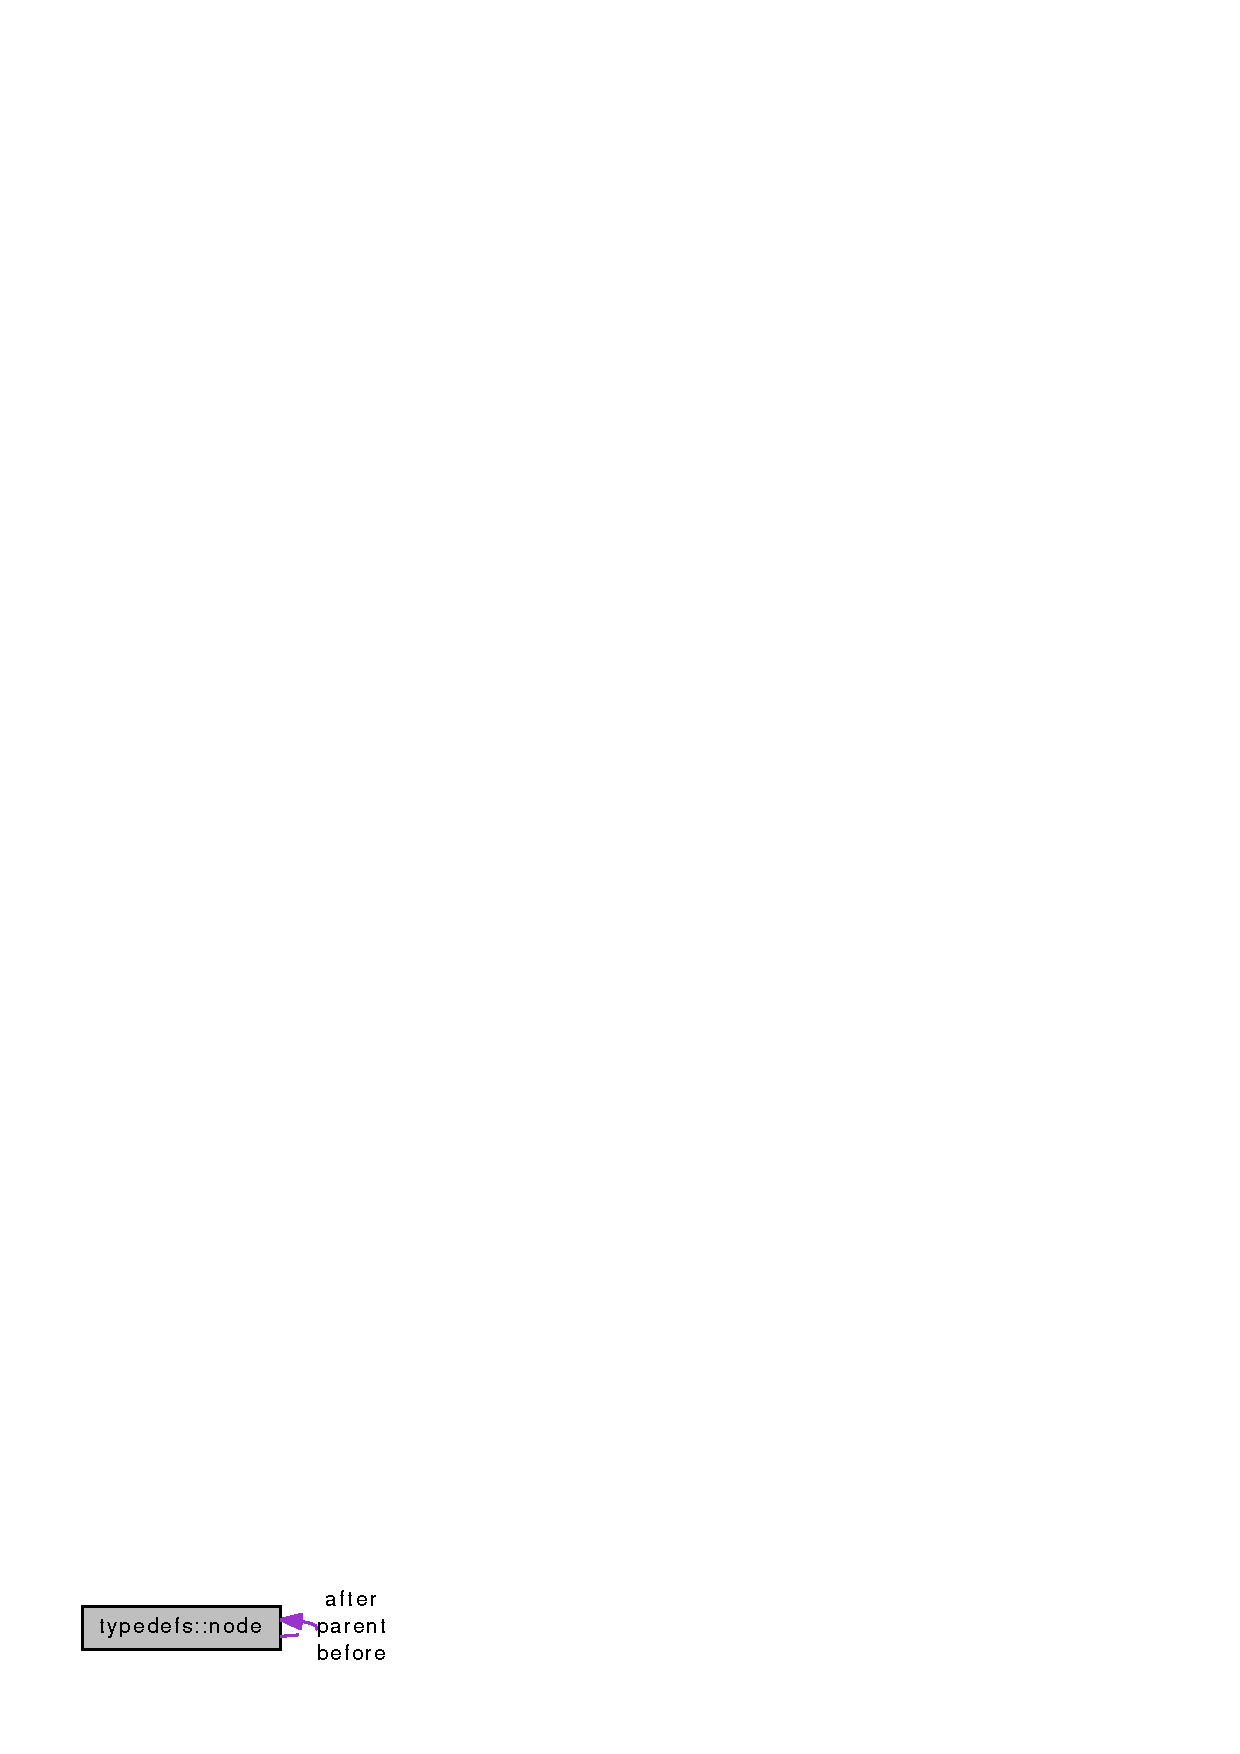
\includegraphics[width=190pt]{typetypedefs_1_1node__coll__graph}
\end{center}
\end{figure}
\subsection*{Public Attributes}
\begin{DoxyCompactItemize}
\item 
LOGICAL \hyperlink{typetypedefs_1_1node_af5be5276f596dfc7b0bc8708399cceab}{normal}
\item 
LOGICAL \hyperlink{typetypedefs_1_1node_a0cb4076931485d693d3f2a06268d99fb}{interstitial}
\item 
DOUBLE PRECISION \hyperlink{typetypedefs_1_1node_a871e2d663d593966f53b92afe0cf7a9d}{wait\_\-time}
\item 
INTEGER \hyperlink{typetypedefs_1_1node_a3d362f7d7c1c7a3313e9da95b07ef2d9}{coord1}
\item 
INTEGER \hyperlink{typetypedefs_1_1node_a193df4b6034deaefb550227844eb14e8}{coord2}
\item 
INTEGER \hyperlink{typetypedefs_1_1node_a549fd6fc277071807eae3dbf96072b2d}{coord3}
\item 
INTEGER \hyperlink{typetypedefs_1_1node_ac16e5faa3b1912530557fe907e0391a6}{sp\_\-num}
\item 
INTEGER \hyperlink{typetypedefs_1_1node_a0ca13f8084895c39c097825fb4675e07}{sec\_\-sp\_\-num}
\item 
INTEGER \hyperlink{typetypedefs_1_1node_ad6a59cc225341281c77e7ffa799a34de}{act\_\-type}
\item 
INTEGER \hyperlink{typetypedefs_1_1node_a6449a053fa7b845ec185aa8beab922ad}{hop\_\-dir}
\item 
TYPE(\hyperlink{typetypedefs_1_1node}{node}), pointer \hyperlink{typetypedefs_1_1node_a3b5c424e056d9e539f9e03279620ae68}{before}
\item 
TYPE(\hyperlink{typetypedefs_1_1node}{node}), pointer \hyperlink{typetypedefs_1_1node_a4bf4e05f8980654446c5f244ba9efbae}{after}
\item 
TYPE(\hyperlink{typetypedefs_1_1node}{node}), pointer \hyperlink{typetypedefs_1_1node_aaf2b0960c972482e99ec436164e05601}{parent}
\item 
INTEGER \hyperlink{typetypedefs_1_1node_a8f68bb360020b240c621a72a7119256d}{leftRight}
\end{DoxyCompactItemize}


\subsection{Detailed Description}


Definition at line 145 of file typedefs.f90.

\subsection{Member Data Documentation}
\hypertarget{typetypedefs_1_1node_ad6a59cc225341281c77e7ffa799a34de}{
\index{typedefs::node@{typedefs::node}!act\_\-type@{act\_\-type}}
\index{act\_\-type@{act\_\-type}!typedefs::node@{typedefs::node}}
\subsubsection[{act\_\-type}]{\setlength{\rightskip}{0pt plus 5cm}INTEGER {\bf typedefs::node::act\_\-type}}}
\label{typetypedefs_1_1node_ad6a59cc225341281c77e7ffa799a34de}


Definition at line 157 of file typedefs.f90.\hypertarget{typetypedefs_1_1node_a4bf4e05f8980654446c5f244ba9efbae}{
\index{typedefs::node@{typedefs::node}!after@{after}}
\index{after@{after}!typedefs::node@{typedefs::node}}
\subsubsection[{after}]{\setlength{\rightskip}{0pt plus 5cm}TYPE ({\bf node}),pointer {\bf typedefs::node::after}}}
\label{typetypedefs_1_1node_a4bf4e05f8980654446c5f244ba9efbae}


Definition at line 160 of file typedefs.f90.\hypertarget{typetypedefs_1_1node_a3b5c424e056d9e539f9e03279620ae68}{
\index{typedefs::node@{typedefs::node}!before@{before}}
\index{before@{before}!typedefs::node@{typedefs::node}}
\subsubsection[{before}]{\setlength{\rightskip}{0pt plus 5cm}TYPE ({\bf node}),pointer {\bf typedefs::node::before}}}
\label{typetypedefs_1_1node_a3b5c424e056d9e539f9e03279620ae68}


Definition at line 159 of file typedefs.f90.\hypertarget{typetypedefs_1_1node_a3d362f7d7c1c7a3313e9da95b07ef2d9}{
\index{typedefs::node@{typedefs::node}!coord1@{coord1}}
\index{coord1@{coord1}!typedefs::node@{typedefs::node}}
\subsubsection[{coord1}]{\setlength{\rightskip}{0pt plus 5cm}INTEGER {\bf typedefs::node::coord1}}}
\label{typetypedefs_1_1node_a3d362f7d7c1c7a3313e9da95b07ef2d9}


Definition at line 152 of file typedefs.f90.\hypertarget{typetypedefs_1_1node_a193df4b6034deaefb550227844eb14e8}{
\index{typedefs::node@{typedefs::node}!coord2@{coord2}}
\index{coord2@{coord2}!typedefs::node@{typedefs::node}}
\subsubsection[{coord2}]{\setlength{\rightskip}{0pt plus 5cm}INTEGER {\bf typedefs::node::coord2}}}
\label{typetypedefs_1_1node_a193df4b6034deaefb550227844eb14e8}


Definition at line 153 of file typedefs.f90.\hypertarget{typetypedefs_1_1node_a549fd6fc277071807eae3dbf96072b2d}{
\index{typedefs::node@{typedefs::node}!coord3@{coord3}}
\index{coord3@{coord3}!typedefs::node@{typedefs::node}}
\subsubsection[{coord3}]{\setlength{\rightskip}{0pt plus 5cm}INTEGER {\bf typedefs::node::coord3}}}
\label{typetypedefs_1_1node_a549fd6fc277071807eae3dbf96072b2d}


Definition at line 154 of file typedefs.f90.\hypertarget{typetypedefs_1_1node_a6449a053fa7b845ec185aa8beab922ad}{
\index{typedefs::node@{typedefs::node}!hop\_\-dir@{hop\_\-dir}}
\index{hop\_\-dir@{hop\_\-dir}!typedefs::node@{typedefs::node}}
\subsubsection[{hop\_\-dir}]{\setlength{\rightskip}{0pt plus 5cm}INTEGER {\bf typedefs::node::hop\_\-dir}}}
\label{typetypedefs_1_1node_a6449a053fa7b845ec185aa8beab922ad}


Definition at line 158 of file typedefs.f90.\hypertarget{typetypedefs_1_1node_a0cb4076931485d693d3f2a06268d99fb}{
\index{typedefs::node@{typedefs::node}!interstitial@{interstitial}}
\index{interstitial@{interstitial}!typedefs::node@{typedefs::node}}
\subsubsection[{interstitial}]{\setlength{\rightskip}{0pt plus 5cm}LOGICAL {\bf typedefs::node::interstitial}}}
\label{typetypedefs_1_1node_a0cb4076931485d693d3f2a06268d99fb}


Definition at line 150 of file typedefs.f90.\hypertarget{typetypedefs_1_1node_a8f68bb360020b240c621a72a7119256d}{
\index{typedefs::node@{typedefs::node}!leftRight@{leftRight}}
\index{leftRight@{leftRight}!typedefs::node@{typedefs::node}}
\subsubsection[{leftRight}]{\setlength{\rightskip}{0pt plus 5cm}INTEGER {\bf typedefs::node::leftRight}}}
\label{typetypedefs_1_1node_a8f68bb360020b240c621a72a7119256d}


Definition at line 162 of file typedefs.f90.\hypertarget{typetypedefs_1_1node_af5be5276f596dfc7b0bc8708399cceab}{
\index{typedefs::node@{typedefs::node}!normal@{normal}}
\index{normal@{normal}!typedefs::node@{typedefs::node}}
\subsubsection[{normal}]{\setlength{\rightskip}{0pt plus 5cm}LOGICAL {\bf typedefs::node::normal}}}
\label{typetypedefs_1_1node_af5be5276f596dfc7b0bc8708399cceab}


Definition at line 149 of file typedefs.f90.\hypertarget{typetypedefs_1_1node_aaf2b0960c972482e99ec436164e05601}{
\index{typedefs::node@{typedefs::node}!parent@{parent}}
\index{parent@{parent}!typedefs::node@{typedefs::node}}
\subsubsection[{parent}]{\setlength{\rightskip}{0pt plus 5cm}TYPE ({\bf node}),pointer {\bf typedefs::node::parent}}}
\label{typetypedefs_1_1node_aaf2b0960c972482e99ec436164e05601}


Definition at line 161 of file typedefs.f90.\hypertarget{typetypedefs_1_1node_a0ca13f8084895c39c097825fb4675e07}{
\index{typedefs::node@{typedefs::node}!sec\_\-sp\_\-num@{sec\_\-sp\_\-num}}
\index{sec\_\-sp\_\-num@{sec\_\-sp\_\-num}!typedefs::node@{typedefs::node}}
\subsubsection[{sec\_\-sp\_\-num}]{\setlength{\rightskip}{0pt plus 5cm}INTEGER {\bf typedefs::node::sec\_\-sp\_\-num}}}
\label{typetypedefs_1_1node_a0ca13f8084895c39c097825fb4675e07}


Definition at line 156 of file typedefs.f90.\hypertarget{typetypedefs_1_1node_ac16e5faa3b1912530557fe907e0391a6}{
\index{typedefs::node@{typedefs::node}!sp\_\-num@{sp\_\-num}}
\index{sp\_\-num@{sp\_\-num}!typedefs::node@{typedefs::node}}
\subsubsection[{sp\_\-num}]{\setlength{\rightskip}{0pt plus 5cm}INTEGER {\bf typedefs::node::sp\_\-num}}}
\label{typetypedefs_1_1node_ac16e5faa3b1912530557fe907e0391a6}


Definition at line 155 of file typedefs.f90.\hypertarget{typetypedefs_1_1node_a871e2d663d593966f53b92afe0cf7a9d}{
\index{typedefs::node@{typedefs::node}!wait\_\-time@{wait\_\-time}}
\index{wait\_\-time@{wait\_\-time}!typedefs::node@{typedefs::node}}
\subsubsection[{wait\_\-time}]{\setlength{\rightskip}{0pt plus 5cm}DOUBLE PRECISION {\bf typedefs::node::wait\_\-time}}}
\label{typetypedefs_1_1node_a871e2d663d593966f53b92afe0cf7a9d}


Definition at line 151 of file typedefs.f90.

The documentation for this type was generated from the following file:\begin{DoxyCompactItemize}
\item 
\hyperlink{typedefs_8f90}{typedefs.f90}\end{DoxyCompactItemize}

\hypertarget{interfacebsimple_1_1OPERATOR_07_4_08}{
\section{bsimple::OPERATOR($>$) Interface Reference}
\label{interfacebsimple_1_1OPERATOR_07_4_08}\index{bsimple::OPERATOR($>$)@{bsimple::OPERATOR($>$)}}
}


\subsection{Detailed Description}


Definition at line 35 of file bsimple.f90.

The documentation for this interface was generated from the following file:\begin{DoxyCompactItemize}
\item 
\hyperlink{bsimple_8f90}{bsimple.f90}\end{DoxyCompactItemize}

\hypertarget{typetypedefs_1_1rate__info}{
\section{typedefs::rate\_\-info Type Reference}
\label{typetypedefs_1_1rate__info}\index{typedefs::rate\_\-info@{typedefs::rate\_\-info}}
}
\subsection*{Public Attributes}
\begin{DoxyCompactItemize}
\item 
INTEGER \hyperlink{typetypedefs_1_1rate__info_a3d8b84c7cd12818e3dbcc846c330d3c2}{r1}
\item 
INTEGER \hyperlink{typetypedefs_1_1rate__info_a4fc3955386c2a940827c6d342f2a31db}{r2}
\item 
INTEGER \hyperlink{typetypedefs_1_1rate__info_a84d556d7f586b962935dcf8ad71eee38}{count}
\end{DoxyCompactItemize}


\subsection{Detailed Description}


Definition at line 14 of file typedefs.f90.

\subsection{Member Data Documentation}
\hypertarget{typetypedefs_1_1rate__info_a84d556d7f586b962935dcf8ad71eee38}{
\index{typedefs::rate\_\-info@{typedefs::rate\_\-info}!count@{count}}
\index{count@{count}!typedefs::rate_info@{typedefs::rate\_\-info}}
\subsubsection[{count}]{\setlength{\rightskip}{0pt plus 5cm}INTEGER {\bf typedefs::rate\_\-info::count}}}
\label{typetypedefs_1_1rate__info_a84d556d7f586b962935dcf8ad71eee38}


Definition at line 20 of file typedefs.f90.\hypertarget{typetypedefs_1_1rate__info_a3d8b84c7cd12818e3dbcc846c330d3c2}{
\index{typedefs::rate\_\-info@{typedefs::rate\_\-info}!r1@{r1}}
\index{r1@{r1}!typedefs::rate_info@{typedefs::rate\_\-info}}
\subsubsection[{r1}]{\setlength{\rightskip}{0pt plus 5cm}INTEGER {\bf typedefs::rate\_\-info::r1}}}
\label{typetypedefs_1_1rate__info_a3d8b84c7cd12818e3dbcc846c330d3c2}


Definition at line 18 of file typedefs.f90.\hypertarget{typetypedefs_1_1rate__info_a4fc3955386c2a940827c6d342f2a31db}{
\index{typedefs::rate\_\-info@{typedefs::rate\_\-info}!r2@{r2}}
\index{r2@{r2}!typedefs::rate_info@{typedefs::rate\_\-info}}
\subsubsection[{r2}]{\setlength{\rightskip}{0pt plus 5cm}INTEGER {\bf typedefs::rate\_\-info::r2}}}
\label{typetypedefs_1_1rate__info_a4fc3955386c2a940827c6d342f2a31db}


Definition at line 19 of file typedefs.f90.

The documentation for this type was generated from the following file:\begin{DoxyCompactItemize}
\item 
\hyperlink{typedefs_8f90}{typedefs.f90}\end{DoxyCompactItemize}

\hypertarget{typetypedefs_1_1reaction}{
\section{typedefs::reaction Type Reference}
\label{typetypedefs_1_1reaction}\index{typedefs::reaction@{typedefs::reaction}}
}
Collaboration diagram for typedefs::reaction:\nopagebreak
\begin{figure}[H]
\begin{center}
\leavevmode
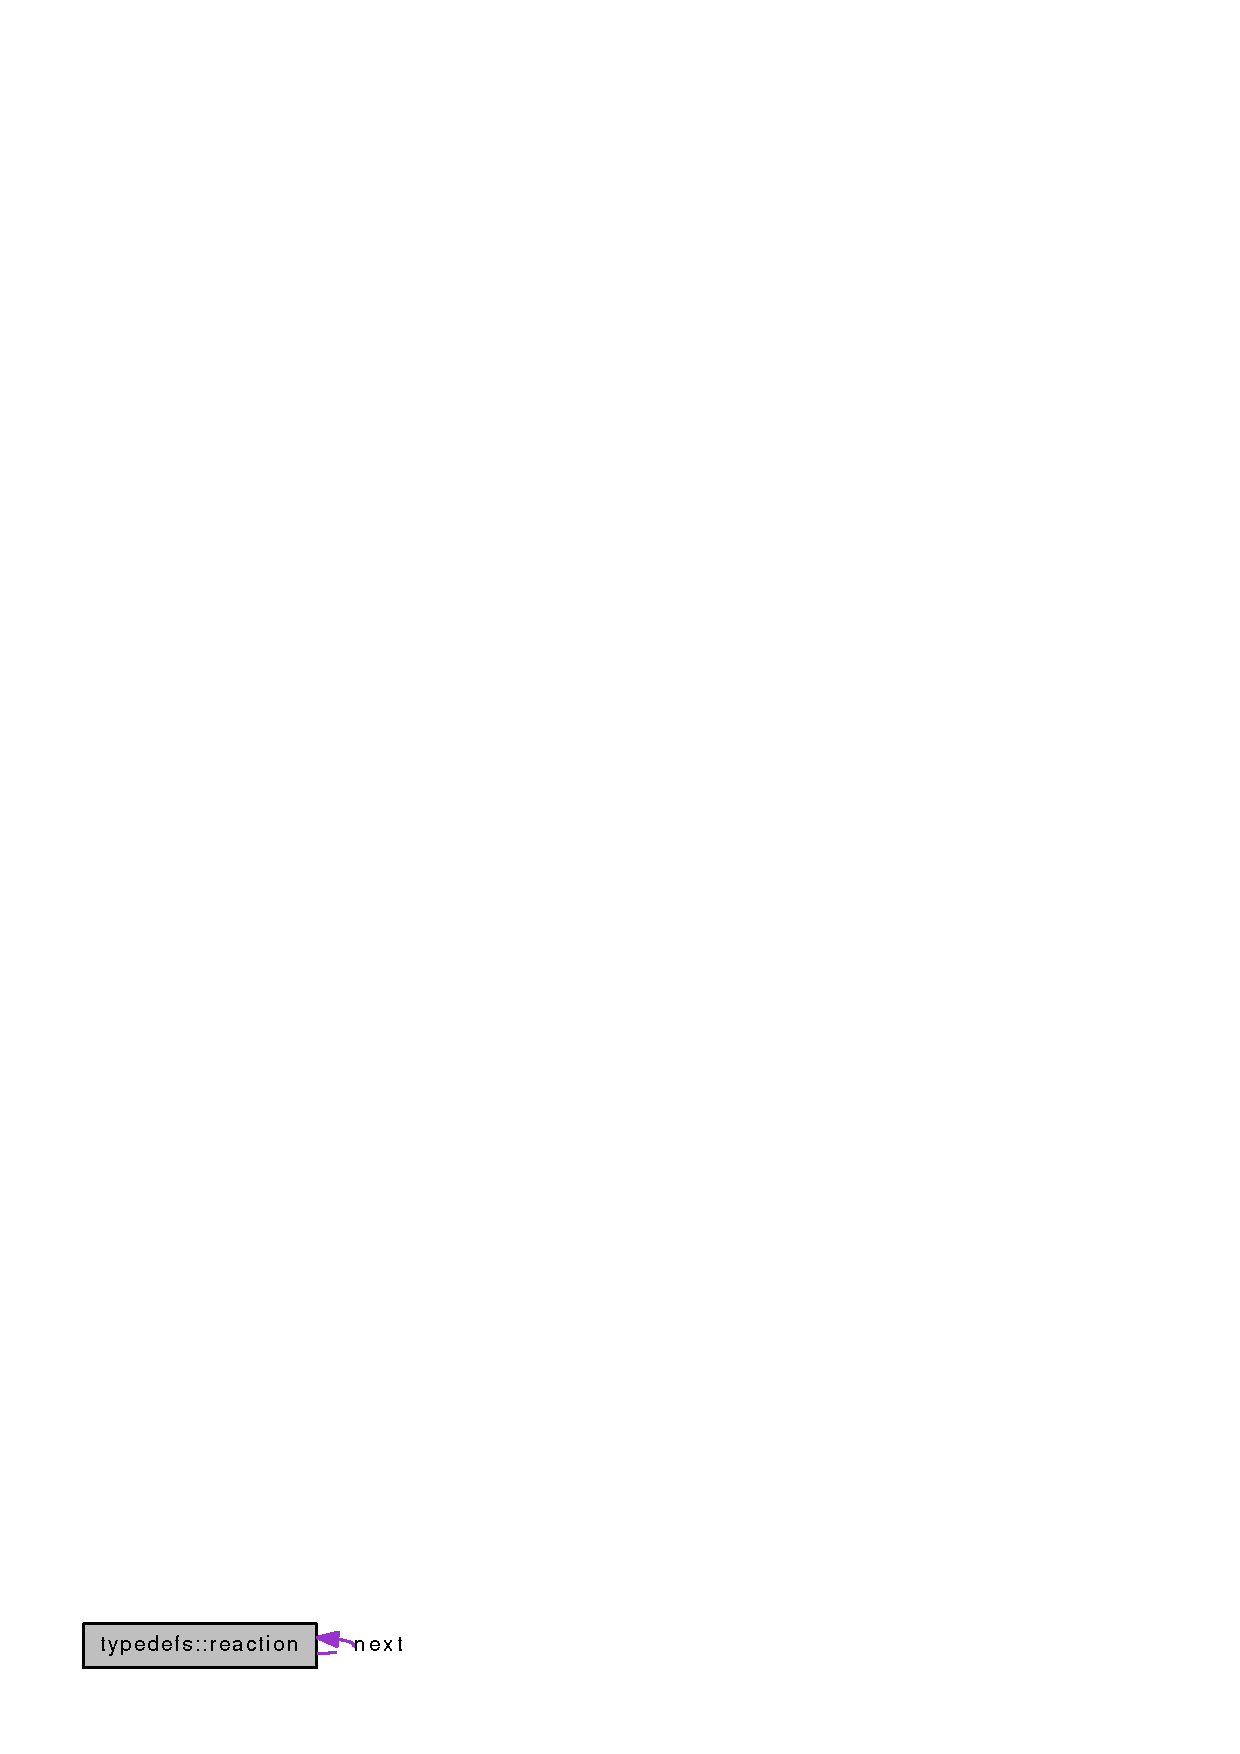
\includegraphics[width=199pt]{typetypedefs_1_1reaction__coll__graph}
\end{center}
\end{figure}
\subsection*{Public Attributes}
\begin{DoxyCompactItemize}
\item 
CHARACTER(len=10) \hyperlink{typetypedefs_1_1reaction_a8aae4f0307c7f74eff0b848511d08f14}{r1}
\item 
CHARACTER(len=10) \hyperlink{typetypedefs_1_1reaction_a9371b4d59c6137afcc8816ddd05ff152}{r2}
\item 
CHARACTER(len=10) \hyperlink{typetypedefs_1_1reaction_aa8086371c87bc65ef845558170090071}{p1}
\item 
CHARACTER(len=10) \hyperlink{typetypedefs_1_1reaction_ace6c8faca4889c014c406c0f76c425e2}{p2}
\item 
CHARACTER(len=10) \hyperlink{typetypedefs_1_1reaction_addfb09d35e61a0dbd2e86644d97d0da2}{p3}
\item 
INTEGER \hyperlink{typetypedefs_1_1reaction_a92444b29e559f93abe272d1279e4d581}{nr1}
\item 
INTEGER \hyperlink{typetypedefs_1_1reaction_a7844e0a4df7c687802872bebb37fd187}{nr2}
\item 
INTEGER \hyperlink{typetypedefs_1_1reaction_ac1c2c1f6500c0af1b6f16cb9d9ed6123}{np1}
\item 
INTEGER \hyperlink{typetypedefs_1_1reaction_a155a3a9ab65f1065cb20ee3b756b222e}{np2}
\item 
INTEGER \hyperlink{typetypedefs_1_1reaction_ac0e23b19e555b458e49a3f2c305fe5e9}{np3}
\item 
integer \hyperlink{typetypedefs_1_1reaction_abf0098a01f9d2604a92c9c009fe5f4cd}{id}
\item 
integer \hyperlink{typetypedefs_1_1reaction_a5cc123e51b6e706aa00a46eb6ca5bddc}{count}
\item 
DOUBLE PRECISION \hyperlink{typetypedefs_1_1reaction_afad3fecf2c6d77ed2ea6b5fa543d5f15}{arrh\_\-alpha}
\item 
DOUBLE PRECISION \hyperlink{typetypedefs_1_1reaction_a60b4e74dafe033970715a08389f88525}{arrh\_\-beta}
\item 
DOUBLE PRECISION \hyperlink{typetypedefs_1_1reaction_a48767e6765b50f472713bcafd23f4252}{arrh\_\-gamma}
\item 
INTEGER \hyperlink{typetypedefs_1_1reaction_a8c84f20b9aa91da88786e437d59eaf93}{rtype}
\item 
TYPE(\hyperlink{typetypedefs_1_1reaction}{reaction}), pointer \hyperlink{typetypedefs_1_1reaction_a6daa057b231b087a532b86ae735acc49}{next}
\end{DoxyCompactItemize}


\subsection{Detailed Description}


Definition at line 177 of file typedefs.f90.

\subsection{Member Data Documentation}
\hypertarget{typetypedefs_1_1reaction_afad3fecf2c6d77ed2ea6b5fa543d5f15}{
\index{typedefs::reaction@{typedefs::reaction}!arrh\_\-alpha@{arrh\_\-alpha}}
\index{arrh\_\-alpha@{arrh\_\-alpha}!typedefs::reaction@{typedefs::reaction}}
\subsubsection[{arrh\_\-alpha}]{\setlength{\rightskip}{0pt plus 5cm}DOUBLE PRECISION {\bf typedefs::reaction::arrh\_\-alpha}}}
\label{typetypedefs_1_1reaction_afad3fecf2c6d77ed2ea6b5fa543d5f15}


Definition at line 190 of file typedefs.f90.\hypertarget{typetypedefs_1_1reaction_a60b4e74dafe033970715a08389f88525}{
\index{typedefs::reaction@{typedefs::reaction}!arrh\_\-beta@{arrh\_\-beta}}
\index{arrh\_\-beta@{arrh\_\-beta}!typedefs::reaction@{typedefs::reaction}}
\subsubsection[{arrh\_\-beta}]{\setlength{\rightskip}{0pt plus 5cm}DOUBLE PRECISION {\bf typedefs::reaction::arrh\_\-beta}}}
\label{typetypedefs_1_1reaction_a60b4e74dafe033970715a08389f88525}


Definition at line 191 of file typedefs.f90.\hypertarget{typetypedefs_1_1reaction_a48767e6765b50f472713bcafd23f4252}{
\index{typedefs::reaction@{typedefs::reaction}!arrh\_\-gamma@{arrh\_\-gamma}}
\index{arrh\_\-gamma@{arrh\_\-gamma}!typedefs::reaction@{typedefs::reaction}}
\subsubsection[{arrh\_\-gamma}]{\setlength{\rightskip}{0pt plus 5cm}DOUBLE PRECISION {\bf typedefs::reaction::arrh\_\-gamma}}}
\label{typetypedefs_1_1reaction_a48767e6765b50f472713bcafd23f4252}


Definition at line 192 of file typedefs.f90.\hypertarget{typetypedefs_1_1reaction_a5cc123e51b6e706aa00a46eb6ca5bddc}{
\index{typedefs::reaction@{typedefs::reaction}!count@{count}}
\index{count@{count}!typedefs::reaction@{typedefs::reaction}}
\subsubsection[{count}]{\setlength{\rightskip}{0pt plus 5cm}integer {\bf typedefs::reaction::count}}}
\label{typetypedefs_1_1reaction_a5cc123e51b6e706aa00a46eb6ca5bddc}


Definition at line 189 of file typedefs.f90.\hypertarget{typetypedefs_1_1reaction_abf0098a01f9d2604a92c9c009fe5f4cd}{
\index{typedefs::reaction@{typedefs::reaction}!id@{id}}
\index{id@{id}!typedefs::reaction@{typedefs::reaction}}
\subsubsection[{id}]{\setlength{\rightskip}{0pt plus 5cm}integer {\bf typedefs::reaction::id}}}
\label{typetypedefs_1_1reaction_abf0098a01f9d2604a92c9c009fe5f4cd}


Definition at line 188 of file typedefs.f90.\hypertarget{typetypedefs_1_1reaction_a6daa057b231b087a532b86ae735acc49}{
\index{typedefs::reaction@{typedefs::reaction}!next@{next}}
\index{next@{next}!typedefs::reaction@{typedefs::reaction}}
\subsubsection[{next}]{\setlength{\rightskip}{0pt plus 5cm}TYPE({\bf reaction}),pointer {\bf typedefs::reaction::next}}}
\label{typetypedefs_1_1reaction_a6daa057b231b087a532b86ae735acc49}


Definition at line 194 of file typedefs.f90.\hypertarget{typetypedefs_1_1reaction_ac1c2c1f6500c0af1b6f16cb9d9ed6123}{
\index{typedefs::reaction@{typedefs::reaction}!np1@{np1}}
\index{np1@{np1}!typedefs::reaction@{typedefs::reaction}}
\subsubsection[{np1}]{\setlength{\rightskip}{0pt plus 5cm}INTEGER {\bf typedefs::reaction::np1}}}
\label{typetypedefs_1_1reaction_ac1c2c1f6500c0af1b6f16cb9d9ed6123}


Definition at line 185 of file typedefs.f90.\hypertarget{typetypedefs_1_1reaction_a155a3a9ab65f1065cb20ee3b756b222e}{
\index{typedefs::reaction@{typedefs::reaction}!np2@{np2}}
\index{np2@{np2}!typedefs::reaction@{typedefs::reaction}}
\subsubsection[{np2}]{\setlength{\rightskip}{0pt plus 5cm}INTEGER {\bf typedefs::reaction::np2}}}
\label{typetypedefs_1_1reaction_a155a3a9ab65f1065cb20ee3b756b222e}


Definition at line 186 of file typedefs.f90.\hypertarget{typetypedefs_1_1reaction_ac0e23b19e555b458e49a3f2c305fe5e9}{
\index{typedefs::reaction@{typedefs::reaction}!np3@{np3}}
\index{np3@{np3}!typedefs::reaction@{typedefs::reaction}}
\subsubsection[{np3}]{\setlength{\rightskip}{0pt plus 5cm}INTEGER {\bf typedefs::reaction::np3}}}
\label{typetypedefs_1_1reaction_ac0e23b19e555b458e49a3f2c305fe5e9}


Definition at line 187 of file typedefs.f90.\hypertarget{typetypedefs_1_1reaction_a92444b29e559f93abe272d1279e4d581}{
\index{typedefs::reaction@{typedefs::reaction}!nr1@{nr1}}
\index{nr1@{nr1}!typedefs::reaction@{typedefs::reaction}}
\subsubsection[{nr1}]{\setlength{\rightskip}{0pt plus 5cm}INTEGER {\bf typedefs::reaction::nr1}}}
\label{typetypedefs_1_1reaction_a92444b29e559f93abe272d1279e4d581}


Definition at line 183 of file typedefs.f90.\hypertarget{typetypedefs_1_1reaction_a7844e0a4df7c687802872bebb37fd187}{
\index{typedefs::reaction@{typedefs::reaction}!nr2@{nr2}}
\index{nr2@{nr2}!typedefs::reaction@{typedefs::reaction}}
\subsubsection[{nr2}]{\setlength{\rightskip}{0pt plus 5cm}INTEGER {\bf typedefs::reaction::nr2}}}
\label{typetypedefs_1_1reaction_a7844e0a4df7c687802872bebb37fd187}


Definition at line 184 of file typedefs.f90.\hypertarget{typetypedefs_1_1reaction_aa8086371c87bc65ef845558170090071}{
\index{typedefs::reaction@{typedefs::reaction}!p1@{p1}}
\index{p1@{p1}!typedefs::reaction@{typedefs::reaction}}
\subsubsection[{p1}]{\setlength{\rightskip}{0pt plus 5cm}CHARACTER(len=10) {\bf typedefs::reaction::p1}}}
\label{typetypedefs_1_1reaction_aa8086371c87bc65ef845558170090071}


Definition at line 180 of file typedefs.f90.\hypertarget{typetypedefs_1_1reaction_ace6c8faca4889c014c406c0f76c425e2}{
\index{typedefs::reaction@{typedefs::reaction}!p2@{p2}}
\index{p2@{p2}!typedefs::reaction@{typedefs::reaction}}
\subsubsection[{p2}]{\setlength{\rightskip}{0pt plus 5cm}CHARACTER(len=10) {\bf typedefs::reaction::p2}}}
\label{typetypedefs_1_1reaction_ace6c8faca4889c014c406c0f76c425e2}


Definition at line 181 of file typedefs.f90.\hypertarget{typetypedefs_1_1reaction_addfb09d35e61a0dbd2e86644d97d0da2}{
\index{typedefs::reaction@{typedefs::reaction}!p3@{p3}}
\index{p3@{p3}!typedefs::reaction@{typedefs::reaction}}
\subsubsection[{p3}]{\setlength{\rightskip}{0pt plus 5cm}CHARACTER(len=10) {\bf typedefs::reaction::p3}}}
\label{typetypedefs_1_1reaction_addfb09d35e61a0dbd2e86644d97d0da2}


Definition at line 182 of file typedefs.f90.\hypertarget{typetypedefs_1_1reaction_a8aae4f0307c7f74eff0b848511d08f14}{
\index{typedefs::reaction@{typedefs::reaction}!r1@{r1}}
\index{r1@{r1}!typedefs::reaction@{typedefs::reaction}}
\subsubsection[{r1}]{\setlength{\rightskip}{0pt plus 5cm}CHARACTER(len=10) {\bf typedefs::reaction::r1}}}
\label{typetypedefs_1_1reaction_a8aae4f0307c7f74eff0b848511d08f14}


Definition at line 178 of file typedefs.f90.\hypertarget{typetypedefs_1_1reaction_a9371b4d59c6137afcc8816ddd05ff152}{
\index{typedefs::reaction@{typedefs::reaction}!r2@{r2}}
\index{r2@{r2}!typedefs::reaction@{typedefs::reaction}}
\subsubsection[{r2}]{\setlength{\rightskip}{0pt plus 5cm}CHARACTER(len=10) {\bf typedefs::reaction::r2}}}
\label{typetypedefs_1_1reaction_a9371b4d59c6137afcc8816ddd05ff152}


Definition at line 179 of file typedefs.f90.\hypertarget{typetypedefs_1_1reaction_a8c84f20b9aa91da88786e437d59eaf93}{
\index{typedefs::reaction@{typedefs::reaction}!rtype@{rtype}}
\index{rtype@{rtype}!typedefs::reaction@{typedefs::reaction}}
\subsubsection[{rtype}]{\setlength{\rightskip}{0pt plus 5cm}INTEGER {\bf typedefs::reaction::rtype}}}
\label{typetypedefs_1_1reaction_a8c84f20b9aa91da88786e437d59eaf93}


Definition at line 193 of file typedefs.f90.

The documentation for this type was generated from the following file:\begin{DoxyCompactItemize}
\item 
\hyperlink{typedefs_8f90}{typedefs.f90}\end{DoxyCompactItemize}

\hypertarget{typenewmod_1_1reaction}{
\section{newmod::reaction Type Reference}
\label{typenewmod_1_1reaction}\index{newmod::reaction@{newmod::reaction}}
}
Collaboration diagram for newmod::reaction:\nopagebreak
\begin{figure}[H]
\begin{center}
\leavevmode
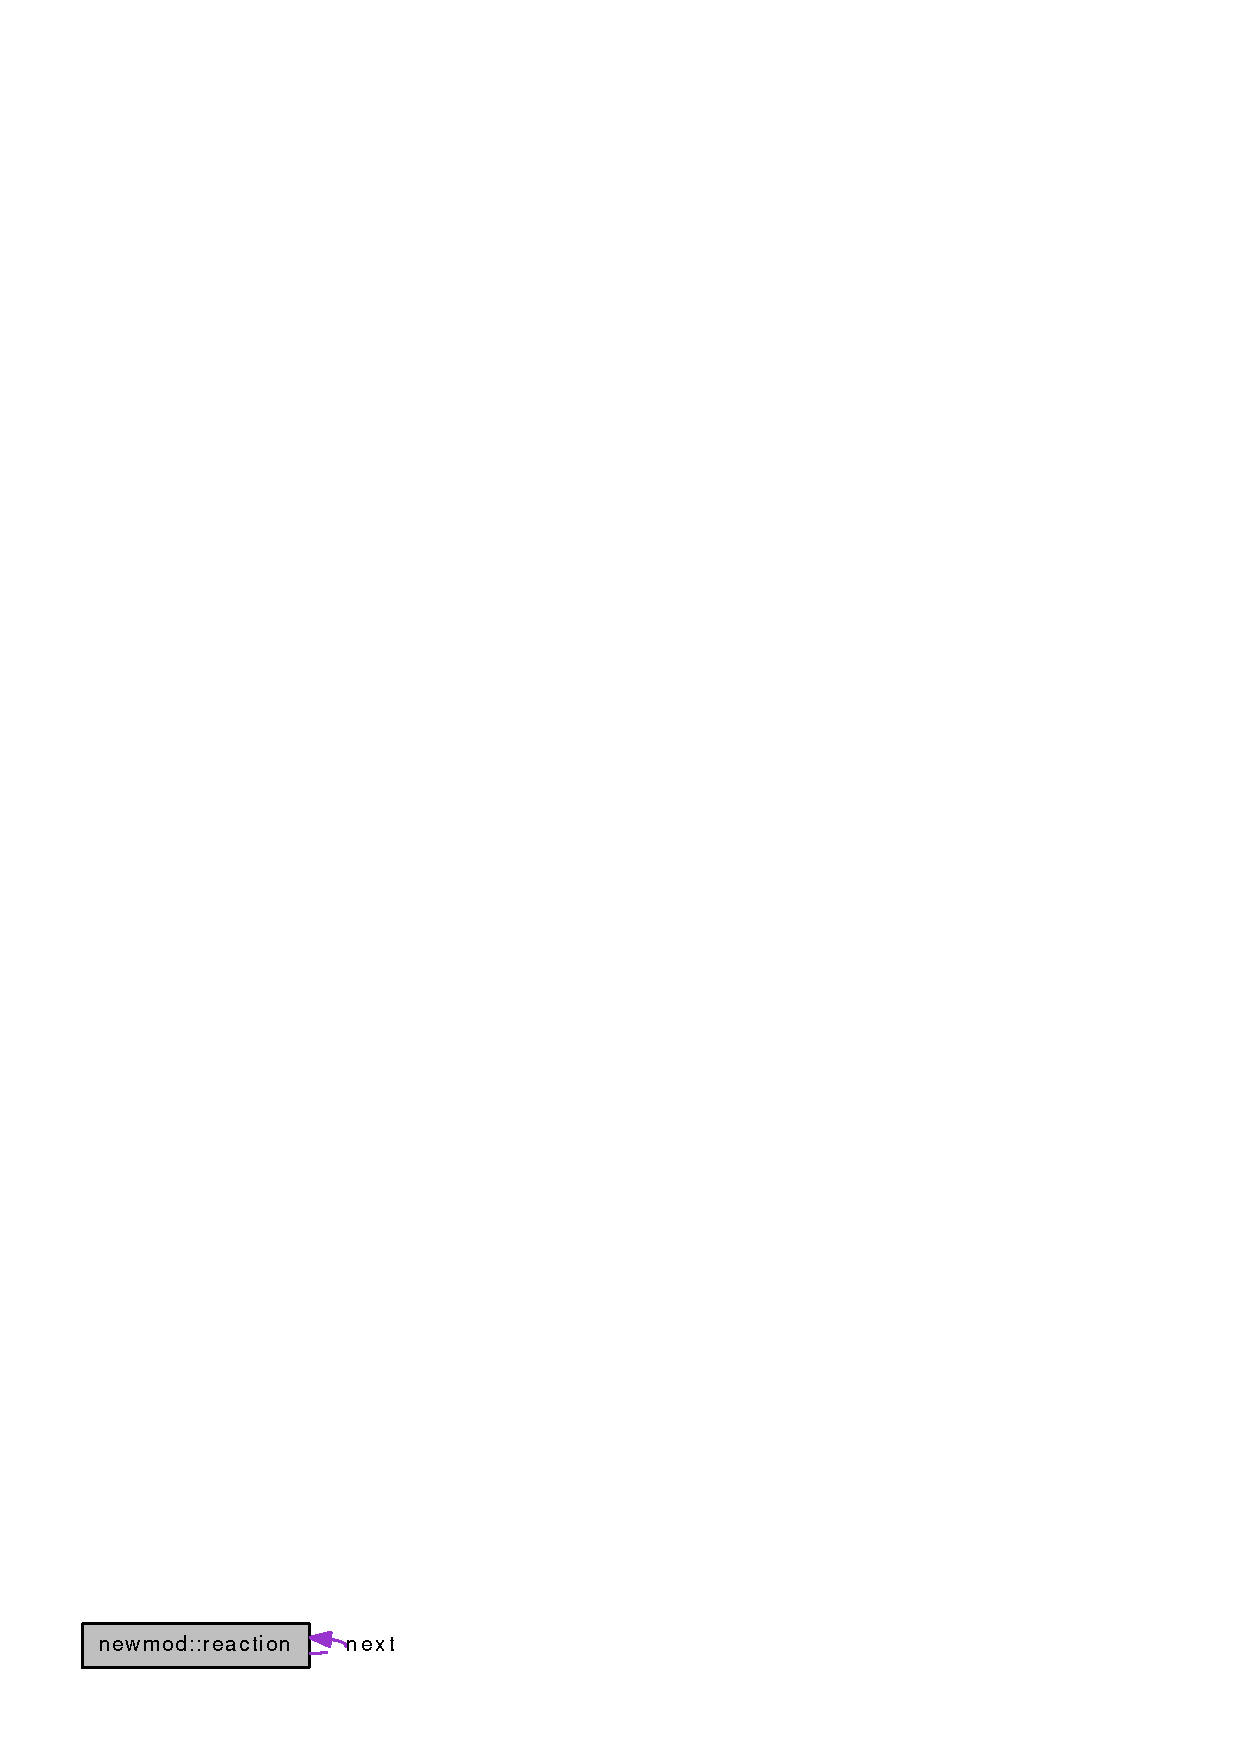
\includegraphics[width=195pt]{typenewmod_1_1reaction__coll__graph}
\end{center}
\end{figure}
\subsection*{Public Attributes}
\begin{DoxyCompactItemize}
\item 
CHARACTER(len=10) \hyperlink{typenewmod_1_1reaction_aae7e300f8eaae407a7014ac8b372b1c7}{r1}
\item 
CHARACTER(len=10) \hyperlink{typenewmod_1_1reaction_accae03e9bc217f2ae538c96f1b303f27}{r2}
\item 
CHARACTER(len=10) \hyperlink{typenewmod_1_1reaction_a4e8c48adbc8bcd0f6dcf2b23563b0362}{p1}
\item 
CHARACTER(len=10) \hyperlink{typenewmod_1_1reaction_ac4e06907f97d8957951ef75a26eefe9e}{p2}
\item 
CHARACTER(len=10) \hyperlink{typenewmod_1_1reaction_a1807db38c60194498e3c737b8ab9be4f}{p3}
\item 
INTEGER \hyperlink{typenewmod_1_1reaction_a773aabf6f76e2e7b82d2418fc3990ec7}{nr1}
\item 
INTEGER \hyperlink{typenewmod_1_1reaction_ae1e0feaf798a9ca8b8fd2e1b7ab20457}{nr2}
\item 
INTEGER \hyperlink{typenewmod_1_1reaction_aaec132a5117781a88da739220d97244a}{np1}
\item 
INTEGER \hyperlink{typenewmod_1_1reaction_aee39c50349fa2f015429286a4d1bc437}{np2}
\item 
INTEGER \hyperlink{typenewmod_1_1reaction_a040ce2d4197a70cff80b26261b7fa961}{np3}
\item 
DOUBLE PRECISION \hyperlink{typenewmod_1_1reaction_ac2450a56db94410d51b2a2f0e200e9c7}{arrh\_\-alpha}
\item 
DOUBLE PRECISION \hyperlink{typenewmod_1_1reaction_a1a4a6b49bbda7af07ab04c808188f3c8}{arrh\_\-beta}
\item 
DOUBLE PRECISION \hyperlink{typenewmod_1_1reaction_aa44c1b0613b29996b884de4123970812}{arrh\_\-gamma}
\item 
INTEGER \hyperlink{typenewmod_1_1reaction_a3f7f53fd5c97562620036f7b3f9da767}{rtype}
\item 
TYPE(\hyperlink{typenewmod_1_1reaction}{reaction}), pointer \hyperlink{typenewmod_1_1reaction_a2089a8cc7dbe8a0e0c8883a67a7041dd}{next}
\end{DoxyCompactItemize}


\subsection{Detailed Description}


Definition at line 13 of file newmod.f90.

\subsection{Member Data Documentation}
\hypertarget{typenewmod_1_1reaction_ac2450a56db94410d51b2a2f0e200e9c7}{
\index{newmod::reaction@{newmod::reaction}!arrh\_\-alpha@{arrh\_\-alpha}}
\index{arrh\_\-alpha@{arrh\_\-alpha}!newmod::reaction@{newmod::reaction}}
\subsubsection[{arrh\_\-alpha}]{\setlength{\rightskip}{0pt plus 5cm}DOUBLE PRECISION {\bf newmod::reaction::arrh\_\-alpha}}}
\label{typenewmod_1_1reaction_ac2450a56db94410d51b2a2f0e200e9c7}


Definition at line 24 of file newmod.f90.\hypertarget{typenewmod_1_1reaction_a1a4a6b49bbda7af07ab04c808188f3c8}{
\index{newmod::reaction@{newmod::reaction}!arrh\_\-beta@{arrh\_\-beta}}
\index{arrh\_\-beta@{arrh\_\-beta}!newmod::reaction@{newmod::reaction}}
\subsubsection[{arrh\_\-beta}]{\setlength{\rightskip}{0pt plus 5cm}DOUBLE PRECISION {\bf newmod::reaction::arrh\_\-beta}}}
\label{typenewmod_1_1reaction_a1a4a6b49bbda7af07ab04c808188f3c8}


Definition at line 25 of file newmod.f90.\hypertarget{typenewmod_1_1reaction_aa44c1b0613b29996b884de4123970812}{
\index{newmod::reaction@{newmod::reaction}!arrh\_\-gamma@{arrh\_\-gamma}}
\index{arrh\_\-gamma@{arrh\_\-gamma}!newmod::reaction@{newmod::reaction}}
\subsubsection[{arrh\_\-gamma}]{\setlength{\rightskip}{0pt plus 5cm}DOUBLE PRECISION {\bf newmod::reaction::arrh\_\-gamma}}}
\label{typenewmod_1_1reaction_aa44c1b0613b29996b884de4123970812}


Definition at line 26 of file newmod.f90.\hypertarget{typenewmod_1_1reaction_a2089a8cc7dbe8a0e0c8883a67a7041dd}{
\index{newmod::reaction@{newmod::reaction}!next@{next}}
\index{next@{next}!newmod::reaction@{newmod::reaction}}
\subsubsection[{next}]{\setlength{\rightskip}{0pt plus 5cm}TYPE({\bf reaction}),pointer {\bf newmod::reaction::next}}}
\label{typenewmod_1_1reaction_a2089a8cc7dbe8a0e0c8883a67a7041dd}


Definition at line 28 of file newmod.f90.\hypertarget{typenewmod_1_1reaction_aaec132a5117781a88da739220d97244a}{
\index{newmod::reaction@{newmod::reaction}!np1@{np1}}
\index{np1@{np1}!newmod::reaction@{newmod::reaction}}
\subsubsection[{np1}]{\setlength{\rightskip}{0pt plus 5cm}INTEGER {\bf newmod::reaction::np1}}}
\label{typenewmod_1_1reaction_aaec132a5117781a88da739220d97244a}


Definition at line 21 of file newmod.f90.\hypertarget{typenewmod_1_1reaction_aee39c50349fa2f015429286a4d1bc437}{
\index{newmod::reaction@{newmod::reaction}!np2@{np2}}
\index{np2@{np2}!newmod::reaction@{newmod::reaction}}
\subsubsection[{np2}]{\setlength{\rightskip}{0pt plus 5cm}INTEGER {\bf newmod::reaction::np2}}}
\label{typenewmod_1_1reaction_aee39c50349fa2f015429286a4d1bc437}


Definition at line 22 of file newmod.f90.\hypertarget{typenewmod_1_1reaction_a040ce2d4197a70cff80b26261b7fa961}{
\index{newmod::reaction@{newmod::reaction}!np3@{np3}}
\index{np3@{np3}!newmod::reaction@{newmod::reaction}}
\subsubsection[{np3}]{\setlength{\rightskip}{0pt plus 5cm}INTEGER {\bf newmod::reaction::np3}}}
\label{typenewmod_1_1reaction_a040ce2d4197a70cff80b26261b7fa961}


Definition at line 23 of file newmod.f90.\hypertarget{typenewmod_1_1reaction_a773aabf6f76e2e7b82d2418fc3990ec7}{
\index{newmod::reaction@{newmod::reaction}!nr1@{nr1}}
\index{nr1@{nr1}!newmod::reaction@{newmod::reaction}}
\subsubsection[{nr1}]{\setlength{\rightskip}{0pt plus 5cm}INTEGER {\bf newmod::reaction::nr1}}}
\label{typenewmod_1_1reaction_a773aabf6f76e2e7b82d2418fc3990ec7}


Definition at line 19 of file newmod.f90.\hypertarget{typenewmod_1_1reaction_ae1e0feaf798a9ca8b8fd2e1b7ab20457}{
\index{newmod::reaction@{newmod::reaction}!nr2@{nr2}}
\index{nr2@{nr2}!newmod::reaction@{newmod::reaction}}
\subsubsection[{nr2}]{\setlength{\rightskip}{0pt plus 5cm}INTEGER {\bf newmod::reaction::nr2}}}
\label{typenewmod_1_1reaction_ae1e0feaf798a9ca8b8fd2e1b7ab20457}


Definition at line 20 of file newmod.f90.\hypertarget{typenewmod_1_1reaction_a4e8c48adbc8bcd0f6dcf2b23563b0362}{
\index{newmod::reaction@{newmod::reaction}!p1@{p1}}
\index{p1@{p1}!newmod::reaction@{newmod::reaction}}
\subsubsection[{p1}]{\setlength{\rightskip}{0pt plus 5cm}CHARACTER(len=10) {\bf newmod::reaction::p1}}}
\label{typenewmod_1_1reaction_a4e8c48adbc8bcd0f6dcf2b23563b0362}


Definition at line 16 of file newmod.f90.\hypertarget{typenewmod_1_1reaction_ac4e06907f97d8957951ef75a26eefe9e}{
\index{newmod::reaction@{newmod::reaction}!p2@{p2}}
\index{p2@{p2}!newmod::reaction@{newmod::reaction}}
\subsubsection[{p2}]{\setlength{\rightskip}{0pt plus 5cm}CHARACTER(len=10) {\bf newmod::reaction::p2}}}
\label{typenewmod_1_1reaction_ac4e06907f97d8957951ef75a26eefe9e}


Definition at line 17 of file newmod.f90.\hypertarget{typenewmod_1_1reaction_a1807db38c60194498e3c737b8ab9be4f}{
\index{newmod::reaction@{newmod::reaction}!p3@{p3}}
\index{p3@{p3}!newmod::reaction@{newmod::reaction}}
\subsubsection[{p3}]{\setlength{\rightskip}{0pt plus 5cm}CHARACTER(len=10) {\bf newmod::reaction::p3}}}
\label{typenewmod_1_1reaction_a1807db38c60194498e3c737b8ab9be4f}


Definition at line 18 of file newmod.f90.\hypertarget{typenewmod_1_1reaction_aae7e300f8eaae407a7014ac8b372b1c7}{
\index{newmod::reaction@{newmod::reaction}!r1@{r1}}
\index{r1@{r1}!newmod::reaction@{newmod::reaction}}
\subsubsection[{r1}]{\setlength{\rightskip}{0pt plus 5cm}CHARACTER(len=10) {\bf newmod::reaction::r1}}}
\label{typenewmod_1_1reaction_aae7e300f8eaae407a7014ac8b372b1c7}


Definition at line 14 of file newmod.f90.\hypertarget{typenewmod_1_1reaction_accae03e9bc217f2ae538c96f1b303f27}{
\index{newmod::reaction@{newmod::reaction}!r2@{r2}}
\index{r2@{r2}!newmod::reaction@{newmod::reaction}}
\subsubsection[{r2}]{\setlength{\rightskip}{0pt plus 5cm}CHARACTER(len=10) {\bf newmod::reaction::r2}}}
\label{typenewmod_1_1reaction_accae03e9bc217f2ae538c96f1b303f27}


Definition at line 15 of file newmod.f90.\hypertarget{typenewmod_1_1reaction_a3f7f53fd5c97562620036f7b3f9da767}{
\index{newmod::reaction@{newmod::reaction}!rtype@{rtype}}
\index{rtype@{rtype}!newmod::reaction@{newmod::reaction}}
\subsubsection[{rtype}]{\setlength{\rightskip}{0pt plus 5cm}INTEGER {\bf newmod::reaction::rtype}}}
\label{typenewmod_1_1reaction_a3f7f53fd5c97562620036f7b3f9da767}


Definition at line 27 of file newmod.f90.

The documentation for this type was generated from the following file:\begin{DoxyCompactItemize}
\item 
\hyperlink{newmod_8f90}{newmod.f90}\end{DoxyCompactItemize}

\hypertarget{typetypedefs_1_1reaction__info}{
\section{typedefs::reaction\_\-info Type Reference}
\label{typetypedefs_1_1reaction__info}\index{typedefs::reaction\_\-info@{typedefs::reaction\_\-info}}
}
\subsection*{Public Attributes}
\begin{DoxyCompactItemize}
\item 
INTEGER \hyperlink{typetypedefs_1_1reaction__info_a003f90458400f3d035bc43e7d7d20525}{nr1}
\item 
INTEGER \hyperlink{typetypedefs_1_1reaction__info_a48ab28601339c673e8ae61c8ab9386b2}{nr2}
\item 
INTEGER \hyperlink{typetypedefs_1_1reaction__info_a416d1c8efe1f3cf0bd338aa6aa405e16}{np1}
\item 
INTEGER \hyperlink{typetypedefs_1_1reaction__info_a33ba0f7158b887f3208dd1e8684e3b04}{np2}
\item 
INTEGER \hyperlink{typetypedefs_1_1reaction__info_a8963dd589f446e518865aebddeb04872}{np3}
\item 
DOUBLE PRECISION \hyperlink{typetypedefs_1_1reaction__info_a9baf1c2bbdf8f0d56fd93342d0a84873}{arrh\_\-alpha}
\item 
DOUBLE PRECISION \hyperlink{typetypedefs_1_1reaction__info_a4b7eb7e54ae72131312af6f924f7e373}{arrh\_\-beta}
\item 
DOUBLE PRECISION \hyperlink{typetypedefs_1_1reaction__info_ab603464ac8abe01ac6567ff26759aad7}{arrh\_\-gamma}
\item 
INTEGER \hyperlink{typetypedefs_1_1reaction__info_a3089ef7ea7760991f09190b030c6c1d1}{rtype}
\item 
integer \hyperlink{typetypedefs_1_1reaction__info_adf314158a153373fe50530ea4765d27b}{id}
\end{DoxyCompactItemize}


\subsection{Detailed Description}


Definition at line 197 of file typedefs.f90.

\subsection{Member Data Documentation}
\hypertarget{typetypedefs_1_1reaction__info_a9baf1c2bbdf8f0d56fd93342d0a84873}{
\index{typedefs::reaction\_\-info@{typedefs::reaction\_\-info}!arrh\_\-alpha@{arrh\_\-alpha}}
\index{arrh\_\-alpha@{arrh\_\-alpha}!typedefs::reaction_info@{typedefs::reaction\_\-info}}
\subsubsection[{arrh\_\-alpha}]{\setlength{\rightskip}{0pt plus 5cm}DOUBLE PRECISION {\bf typedefs::reaction\_\-info::arrh\_\-alpha}}}
\label{typetypedefs_1_1reaction__info_a9baf1c2bbdf8f0d56fd93342d0a84873}


Definition at line 203 of file typedefs.f90.\hypertarget{typetypedefs_1_1reaction__info_a4b7eb7e54ae72131312af6f924f7e373}{
\index{typedefs::reaction\_\-info@{typedefs::reaction\_\-info}!arrh\_\-beta@{arrh\_\-beta}}
\index{arrh\_\-beta@{arrh\_\-beta}!typedefs::reaction_info@{typedefs::reaction\_\-info}}
\subsubsection[{arrh\_\-beta}]{\setlength{\rightskip}{0pt plus 5cm}DOUBLE PRECISION {\bf typedefs::reaction\_\-info::arrh\_\-beta}}}
\label{typetypedefs_1_1reaction__info_a4b7eb7e54ae72131312af6f924f7e373}


Definition at line 204 of file typedefs.f90.\hypertarget{typetypedefs_1_1reaction__info_ab603464ac8abe01ac6567ff26759aad7}{
\index{typedefs::reaction\_\-info@{typedefs::reaction\_\-info}!arrh\_\-gamma@{arrh\_\-gamma}}
\index{arrh\_\-gamma@{arrh\_\-gamma}!typedefs::reaction_info@{typedefs::reaction\_\-info}}
\subsubsection[{arrh\_\-gamma}]{\setlength{\rightskip}{0pt plus 5cm}DOUBLE PRECISION {\bf typedefs::reaction\_\-info::arrh\_\-gamma}}}
\label{typetypedefs_1_1reaction__info_ab603464ac8abe01ac6567ff26759aad7}


Definition at line 205 of file typedefs.f90.\hypertarget{typetypedefs_1_1reaction__info_adf314158a153373fe50530ea4765d27b}{
\index{typedefs::reaction\_\-info@{typedefs::reaction\_\-info}!id@{id}}
\index{id@{id}!typedefs::reaction_info@{typedefs::reaction\_\-info}}
\subsubsection[{id}]{\setlength{\rightskip}{0pt plus 5cm}integer {\bf typedefs::reaction\_\-info::id}}}
\label{typetypedefs_1_1reaction__info_adf314158a153373fe50530ea4765d27b}


Definition at line 207 of file typedefs.f90.\hypertarget{typetypedefs_1_1reaction__info_a416d1c8efe1f3cf0bd338aa6aa405e16}{
\index{typedefs::reaction\_\-info@{typedefs::reaction\_\-info}!np1@{np1}}
\index{np1@{np1}!typedefs::reaction_info@{typedefs::reaction\_\-info}}
\subsubsection[{np1}]{\setlength{\rightskip}{0pt plus 5cm}INTEGER {\bf typedefs::reaction\_\-info::np1}}}
\label{typetypedefs_1_1reaction__info_a416d1c8efe1f3cf0bd338aa6aa405e16}


Definition at line 200 of file typedefs.f90.\hypertarget{typetypedefs_1_1reaction__info_a33ba0f7158b887f3208dd1e8684e3b04}{
\index{typedefs::reaction\_\-info@{typedefs::reaction\_\-info}!np2@{np2}}
\index{np2@{np2}!typedefs::reaction_info@{typedefs::reaction\_\-info}}
\subsubsection[{np2}]{\setlength{\rightskip}{0pt plus 5cm}INTEGER {\bf typedefs::reaction\_\-info::np2}}}
\label{typetypedefs_1_1reaction__info_a33ba0f7158b887f3208dd1e8684e3b04}


Definition at line 201 of file typedefs.f90.\hypertarget{typetypedefs_1_1reaction__info_a8963dd589f446e518865aebddeb04872}{
\index{typedefs::reaction\_\-info@{typedefs::reaction\_\-info}!np3@{np3}}
\index{np3@{np3}!typedefs::reaction_info@{typedefs::reaction\_\-info}}
\subsubsection[{np3}]{\setlength{\rightskip}{0pt plus 5cm}INTEGER {\bf typedefs::reaction\_\-info::np3}}}
\label{typetypedefs_1_1reaction__info_a8963dd589f446e518865aebddeb04872}


Definition at line 202 of file typedefs.f90.\hypertarget{typetypedefs_1_1reaction__info_a003f90458400f3d035bc43e7d7d20525}{
\index{typedefs::reaction\_\-info@{typedefs::reaction\_\-info}!nr1@{nr1}}
\index{nr1@{nr1}!typedefs::reaction_info@{typedefs::reaction\_\-info}}
\subsubsection[{nr1}]{\setlength{\rightskip}{0pt plus 5cm}INTEGER {\bf typedefs::reaction\_\-info::nr1}}}
\label{typetypedefs_1_1reaction__info_a003f90458400f3d035bc43e7d7d20525}


Definition at line 198 of file typedefs.f90.\hypertarget{typetypedefs_1_1reaction__info_a48ab28601339c673e8ae61c8ab9386b2}{
\index{typedefs::reaction\_\-info@{typedefs::reaction\_\-info}!nr2@{nr2}}
\index{nr2@{nr2}!typedefs::reaction_info@{typedefs::reaction\_\-info}}
\subsubsection[{nr2}]{\setlength{\rightskip}{0pt plus 5cm}INTEGER {\bf typedefs::reaction\_\-info::nr2}}}
\label{typetypedefs_1_1reaction__info_a48ab28601339c673e8ae61c8ab9386b2}


Definition at line 199 of file typedefs.f90.\hypertarget{typetypedefs_1_1reaction__info_a3089ef7ea7760991f09190b030c6c1d1}{
\index{typedefs::reaction\_\-info@{typedefs::reaction\_\-info}!rtype@{rtype}}
\index{rtype@{rtype}!typedefs::reaction_info@{typedefs::reaction\_\-info}}
\subsubsection[{rtype}]{\setlength{\rightskip}{0pt plus 5cm}INTEGER {\bf typedefs::reaction\_\-info::rtype}}}
\label{typetypedefs_1_1reaction__info_a3089ef7ea7760991f09190b030c6c1d1}


Definition at line 206 of file typedefs.f90.

The documentation for this type was generated from the following file:\begin{DoxyCompactItemize}
\item 
\hyperlink{typedefs_8f90}{typedefs.f90}\end{DoxyCompactItemize}

\hypertarget{typetypedefs_1_1se__info}{
\section{typedefs::se\_\-info Type Reference}
\label{typetypedefs_1_1se__info}\index{typedefs::se\_\-info@{typedefs::se\_\-info}}
}
Collaboration diagram for typedefs::se\_\-info:\nopagebreak
\begin{figure}[H]
\begin{center}
\leavevmode
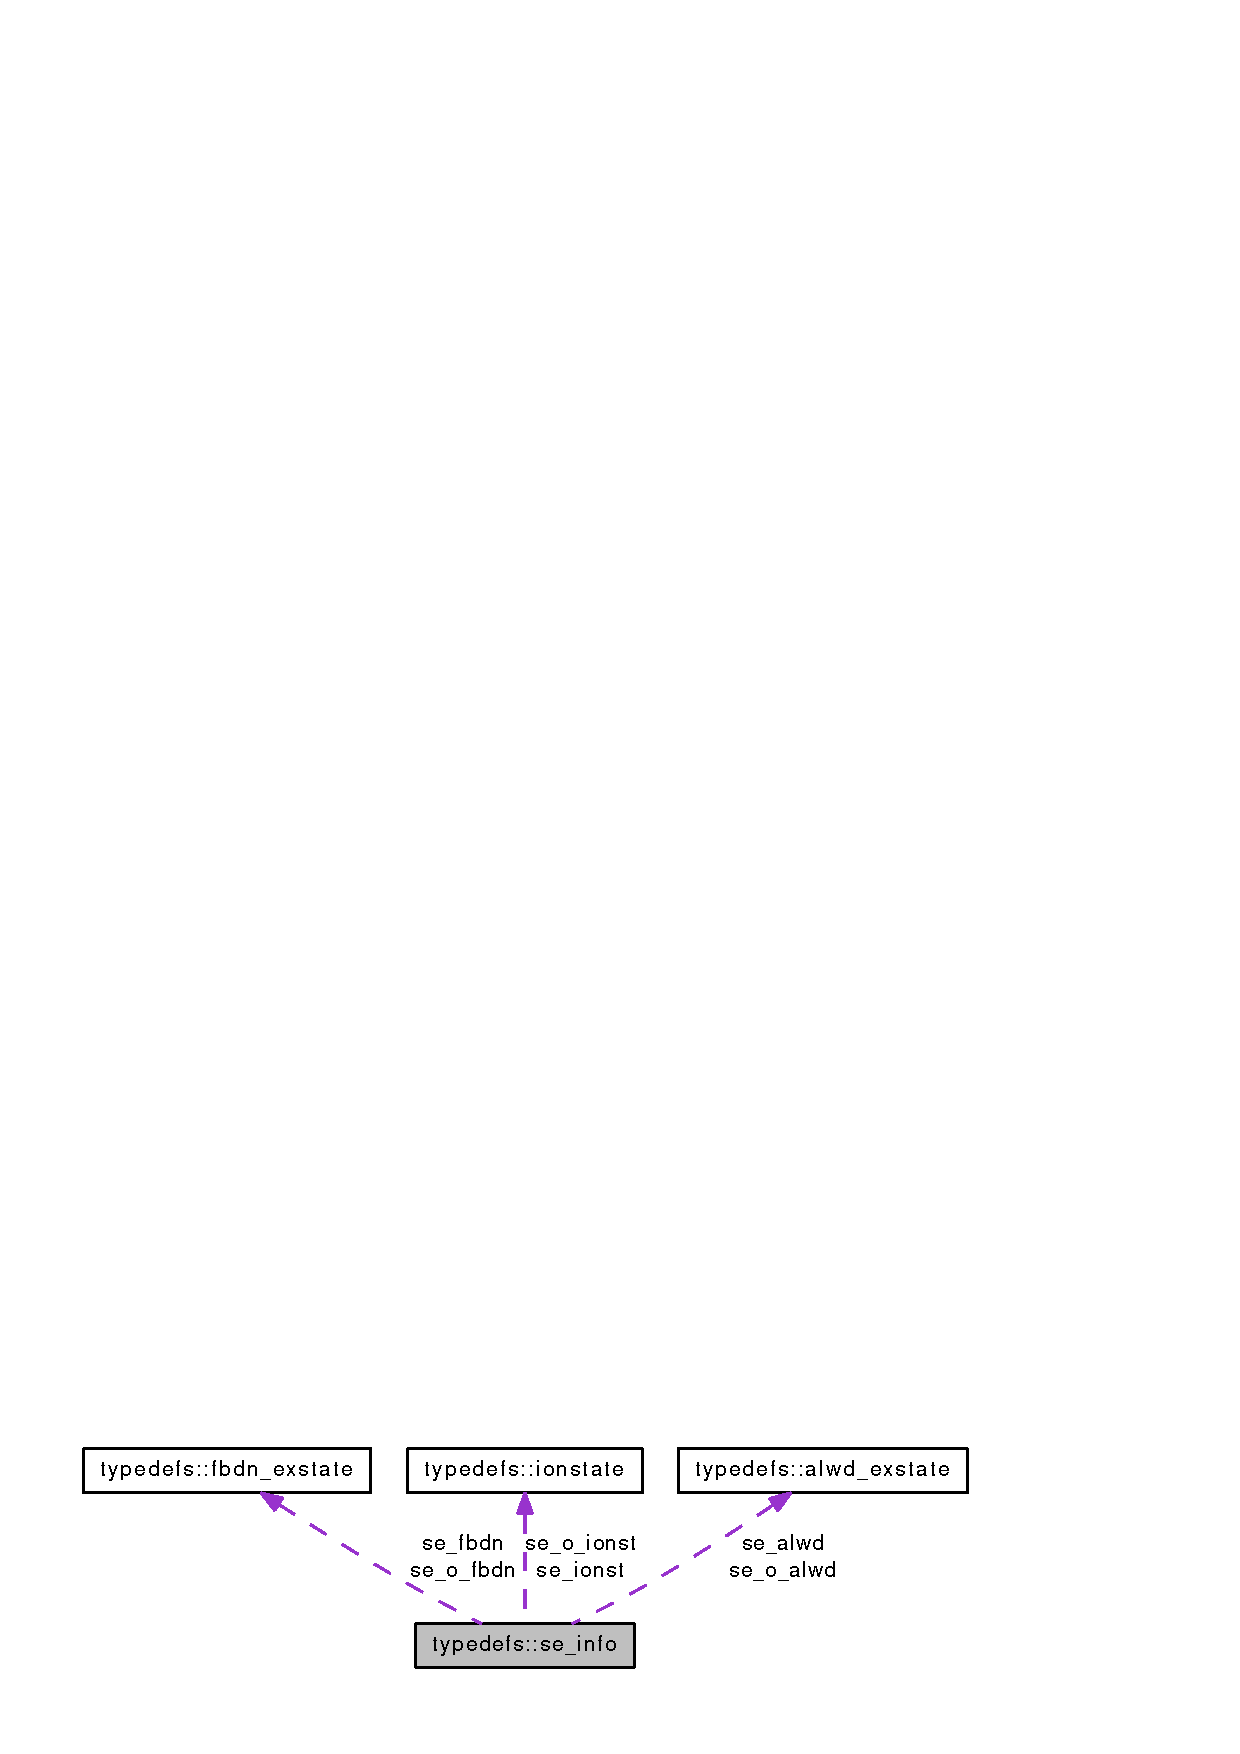
\includegraphics[width=400pt]{typetypedefs_1_1se__info__coll__graph}
\end{center}
\end{figure}
\subsection*{Public Attributes}
\begin{DoxyCompactItemize}
\item 
INTEGER \hyperlink{typetypedefs_1_1se__info_aa87601b1b02d6f3982236107d5cdc350}{generation}
\item 
DOUBLE PRECISION \hyperlink{typetypedefs_1_1se__info_a1cb4fd9197cbe6e491f8c015385d3983}{se\_\-energy}
\item 
DOUBLE PRECISION \hyperlink{typetypedefs_1_1se__info_a03b3420231fce0a9fdd58f4579b45700}{se\_\-iontot}
\item 
DOUBLE PRECISION \hyperlink{typetypedefs_1_1se__info_aaeb12f09d4e2ae1f4545c2a9ee1b3b88}{se\_\-extot}
\item 
DOUBLE PRECISION \hyperlink{typetypedefs_1_1se__info_a7be9da23a41fbccf4dc5c0d157ef63e9}{se\_\-ineltot}
\item 
DOUBLE PRECISION \hyperlink{typetypedefs_1_1se__info_a2df8b473f04eca6790c23fcf8721af2d}{se\_\-alwd\_\-extot}
\item 
DOUBLE PRECISION \hyperlink{typetypedefs_1_1se__info_a83ca0f6f1df82c84b483903bf0744388}{se\_\-fbdn\_\-extot}
\item 
DOUBLE PRECISION \hyperlink{typetypedefs_1_1se__info_ab88b1c65d29fd5dd0e82f1fcf0365a34}{se\_\-o\_\-iontot}
\item 
DOUBLE PRECISION \hyperlink{typetypedefs_1_1se__info_a4619ac26e35125680fe8e38428eae0b9}{se\_\-o\_\-extot}
\item 
DOUBLE PRECISION \hyperlink{typetypedefs_1_1se__info_a44003d458c89fc0931faf433b0b6f50c}{se\_\-o\_\-ineltot}
\item 
DOUBLE PRECISION \hyperlink{typetypedefs_1_1se__info_a1aa742b3b6d98a4de72c0232f9c2e2b1}{se\_\-o\_\-alwd\_\-extot}
\item 
DOUBLE PRECISION \hyperlink{typetypedefs_1_1se__info_a85c6182ccd3f9e49ece87ac7ec2d8e97}{se\_\-o\_\-fbdn\_\-extot}
\item 
DOUBLE PRECISION \hyperlink{typetypedefs_1_1se__info_ae366af38541d327018e02f7c121d2fed}{se\_\-o3\_\-extot}
\item 
DOUBLE PRECISION \hyperlink{typetypedefs_1_1se__info_aae367a6217e2ba4848d64c1f37b692d2}{se\_\-o3\_\-iontot}
\item 
INTEGER, dimension(3) \hyperlink{typetypedefs_1_1se__info_a8bd5d9742b432404882c43eeb9378ef5}{parent\_\-coords}
\item 
TYPE(\hyperlink{typetypedefs_1_1ionstate}{ionstate}), dimension(:), allocatable \hyperlink{typetypedefs_1_1se__info_a791773634dc97c66c0792489bc139f4a}{se\_\-ionst}
\item 
TYPE(\hyperlink{typetypedefs_1_1alwd__exstate}{alwd\_\-exstate}), dimension(:), allocatable \hyperlink{typetypedefs_1_1se__info_a208e6628ee7993cd5df24be28c3835fc}{se\_\-alwd}
\item 
TYPE(\hyperlink{typetypedefs_1_1fbdn__exstate}{fbdn\_\-exstate}), dimension(:), allocatable \hyperlink{typetypedefs_1_1se__info_ae86fd99616525aef71601e1c8036f11a}{se\_\-fbdn}
\item 
TYPE(\hyperlink{typetypedefs_1_1ionstate}{ionstate}), dimension(:), allocatable \hyperlink{typetypedefs_1_1se__info_abba4b9ad7d6f0faa147726c8a41903d0}{se\_\-o\_\-ionst}
\item 
TYPE(\hyperlink{typetypedefs_1_1alwd__exstate}{alwd\_\-exstate}), dimension(:), allocatable \hyperlink{typetypedefs_1_1se__info_a838335cf3aac3f755cf712eafa14c9e0}{se\_\-o\_\-alwd}
\item 
TYPE(\hyperlink{typetypedefs_1_1fbdn__exstate}{fbdn\_\-exstate}), dimension(:), allocatable \hyperlink{typetypedefs_1_1se__info_a5acf75a4e3c255609d5d7b6e079e2ef1}{se\_\-o\_\-fbdn}
\item 
DOUBLE PRECISION, dimension(:), allocatable \hyperlink{typetypedefs_1_1se__info_a22bb3ce5a09c2ad12c553e3b427ec812}{se\_\-ionsigs}
\item 
DOUBLE PRECISION, dimension(:), allocatable \hyperlink{typetypedefs_1_1se__info_a8d0aa801ea2e0abab6173ad6eb3310c1}{se\_\-alwdsigs}
\item 
DOUBLE PRECISION, dimension(:), allocatable \hyperlink{typetypedefs_1_1se__info_a358b552703647e88a165b6523d1e4daa}{se\_\-fbdnsigs}
\item 
DOUBLE PRECISION, dimension(:), allocatable \hyperlink{typetypedefs_1_1se__info_adace414a14734324000a3b05920e1c3d}{se\_\-o\_\-ionsigs}
\item 
DOUBLE PRECISION, dimension(:), allocatable \hyperlink{typetypedefs_1_1se__info_a0b5d9872f495081658c1545f6b014a08}{se\_\-o\_\-alwdsigs}
\item 
DOUBLE PRECISION, dimension(:), allocatable \hyperlink{typetypedefs_1_1se__info_a12be38b49ef5d0878b370e8f15737e0f}{se\_\-o\_\-fbdnsigs}
\end{DoxyCompactItemize}


\subsection{Detailed Description}


Definition at line 108 of file typedefs.f90.

\subsection{Member Data Documentation}
\hypertarget{typetypedefs_1_1se__info_aa87601b1b02d6f3982236107d5cdc350}{
\index{typedefs::se\_\-info@{typedefs::se\_\-info}!generation@{generation}}
\index{generation@{generation}!typedefs::se_info@{typedefs::se\_\-info}}
\subsubsection[{generation}]{\setlength{\rightskip}{0pt plus 5cm}INTEGER {\bf typedefs::se\_\-info::generation}}}
\label{typetypedefs_1_1se__info_aa87601b1b02d6f3982236107d5cdc350}


Definition at line 115 of file typedefs.f90.\hypertarget{typetypedefs_1_1se__info_a8bd5d9742b432404882c43eeb9378ef5}{
\index{typedefs::se\_\-info@{typedefs::se\_\-info}!parent\_\-coords@{parent\_\-coords}}
\index{parent\_\-coords@{parent\_\-coords}!typedefs::se_info@{typedefs::se\_\-info}}
\subsubsection[{parent\_\-coords}]{\setlength{\rightskip}{0pt plus 5cm}INTEGER,dimension(3) {\bf typedefs::se\_\-info::parent\_\-coords}}}
\label{typetypedefs_1_1se__info_a8bd5d9742b432404882c43eeb9378ef5}


Definition at line 129 of file typedefs.f90.\hypertarget{typetypedefs_1_1se__info_a208e6628ee7993cd5df24be28c3835fc}{
\index{typedefs::se\_\-info@{typedefs::se\_\-info}!se\_\-alwd@{se\_\-alwd}}
\index{se\_\-alwd@{se\_\-alwd}!typedefs::se_info@{typedefs::se\_\-info}}
\subsubsection[{se\_\-alwd}]{\setlength{\rightskip}{0pt plus 5cm}TYPE({\bf alwd\_\-exstate}),dimension(:),allocatable {\bf typedefs::se\_\-info::se\_\-alwd}}}
\label{typetypedefs_1_1se__info_a208e6628ee7993cd5df24be28c3835fc}


Definition at line 131 of file typedefs.f90.\hypertarget{typetypedefs_1_1se__info_a2df8b473f04eca6790c23fcf8721af2d}{
\index{typedefs::se\_\-info@{typedefs::se\_\-info}!se\_\-alwd\_\-extot@{se\_\-alwd\_\-extot}}
\index{se\_\-alwd\_\-extot@{se\_\-alwd\_\-extot}!typedefs::se_info@{typedefs::se\_\-info}}
\subsubsection[{se\_\-alwd\_\-extot}]{\setlength{\rightskip}{0pt plus 5cm}DOUBLE PRECISION {\bf typedefs::se\_\-info::se\_\-alwd\_\-extot}}}
\label{typetypedefs_1_1se__info_a2df8b473f04eca6790c23fcf8721af2d}


Definition at line 120 of file typedefs.f90.\hypertarget{typetypedefs_1_1se__info_a8d0aa801ea2e0abab6173ad6eb3310c1}{
\index{typedefs::se\_\-info@{typedefs::se\_\-info}!se\_\-alwdsigs@{se\_\-alwdsigs}}
\index{se\_\-alwdsigs@{se\_\-alwdsigs}!typedefs::se_info@{typedefs::se\_\-info}}
\subsubsection[{se\_\-alwdsigs}]{\setlength{\rightskip}{0pt plus 5cm}DOUBLE PRECISION,dimension(:),allocatable {\bf typedefs::se\_\-info::se\_\-alwdsigs}}}
\label{typetypedefs_1_1se__info_a8d0aa801ea2e0abab6173ad6eb3310c1}


Definition at line 137 of file typedefs.f90.\hypertarget{typetypedefs_1_1se__info_a1cb4fd9197cbe6e491f8c015385d3983}{
\index{typedefs::se\_\-info@{typedefs::se\_\-info}!se\_\-energy@{se\_\-energy}}
\index{se\_\-energy@{se\_\-energy}!typedefs::se_info@{typedefs::se\_\-info}}
\subsubsection[{se\_\-energy}]{\setlength{\rightskip}{0pt plus 5cm}DOUBLE PRECISION {\bf typedefs::se\_\-info::se\_\-energy}}}
\label{typetypedefs_1_1se__info_a1cb4fd9197cbe6e491f8c015385d3983}


Definition at line 116 of file typedefs.f90.\hypertarget{typetypedefs_1_1se__info_aaeb12f09d4e2ae1f4545c2a9ee1b3b88}{
\index{typedefs::se\_\-info@{typedefs::se\_\-info}!se\_\-extot@{se\_\-extot}}
\index{se\_\-extot@{se\_\-extot}!typedefs::se_info@{typedefs::se\_\-info}}
\subsubsection[{se\_\-extot}]{\setlength{\rightskip}{0pt plus 5cm}DOUBLE PRECISION {\bf typedefs::se\_\-info::se\_\-extot}}}
\label{typetypedefs_1_1se__info_aaeb12f09d4e2ae1f4545c2a9ee1b3b88}


Definition at line 118 of file typedefs.f90.\hypertarget{typetypedefs_1_1se__info_ae86fd99616525aef71601e1c8036f11a}{
\index{typedefs::se\_\-info@{typedefs::se\_\-info}!se\_\-fbdn@{se\_\-fbdn}}
\index{se\_\-fbdn@{se\_\-fbdn}!typedefs::se_info@{typedefs::se\_\-info}}
\subsubsection[{se\_\-fbdn}]{\setlength{\rightskip}{0pt plus 5cm}TYPE({\bf fbdn\_\-exstate}),dimension(:),allocatable {\bf typedefs::se\_\-info::se\_\-fbdn}}}
\label{typetypedefs_1_1se__info_ae86fd99616525aef71601e1c8036f11a}


Definition at line 132 of file typedefs.f90.\hypertarget{typetypedefs_1_1se__info_a83ca0f6f1df82c84b483903bf0744388}{
\index{typedefs::se\_\-info@{typedefs::se\_\-info}!se\_\-fbdn\_\-extot@{se\_\-fbdn\_\-extot}}
\index{se\_\-fbdn\_\-extot@{se\_\-fbdn\_\-extot}!typedefs::se_info@{typedefs::se\_\-info}}
\subsubsection[{se\_\-fbdn\_\-extot}]{\setlength{\rightskip}{0pt plus 5cm}DOUBLE PRECISION {\bf typedefs::se\_\-info::se\_\-fbdn\_\-extot}}}
\label{typetypedefs_1_1se__info_a83ca0f6f1df82c84b483903bf0744388}


Definition at line 121 of file typedefs.f90.\hypertarget{typetypedefs_1_1se__info_a358b552703647e88a165b6523d1e4daa}{
\index{typedefs::se\_\-info@{typedefs::se\_\-info}!se\_\-fbdnsigs@{se\_\-fbdnsigs}}
\index{se\_\-fbdnsigs@{se\_\-fbdnsigs}!typedefs::se_info@{typedefs::se\_\-info}}
\subsubsection[{se\_\-fbdnsigs}]{\setlength{\rightskip}{0pt plus 5cm}DOUBLE PRECISION,dimension(:),allocatable {\bf typedefs::se\_\-info::se\_\-fbdnsigs}}}
\label{typetypedefs_1_1se__info_a358b552703647e88a165b6523d1e4daa}


Definition at line 138 of file typedefs.f90.\hypertarget{typetypedefs_1_1se__info_a7be9da23a41fbccf4dc5c0d157ef63e9}{
\index{typedefs::se\_\-info@{typedefs::se\_\-info}!se\_\-ineltot@{se\_\-ineltot}}
\index{se\_\-ineltot@{se\_\-ineltot}!typedefs::se_info@{typedefs::se\_\-info}}
\subsubsection[{se\_\-ineltot}]{\setlength{\rightskip}{0pt plus 5cm}DOUBLE PRECISION {\bf typedefs::se\_\-info::se\_\-ineltot}}}
\label{typetypedefs_1_1se__info_a7be9da23a41fbccf4dc5c0d157ef63e9}


Definition at line 119 of file typedefs.f90.\hypertarget{typetypedefs_1_1se__info_a22bb3ce5a09c2ad12c553e3b427ec812}{
\index{typedefs::se\_\-info@{typedefs::se\_\-info}!se\_\-ionsigs@{se\_\-ionsigs}}
\index{se\_\-ionsigs@{se\_\-ionsigs}!typedefs::se_info@{typedefs::se\_\-info}}
\subsubsection[{se\_\-ionsigs}]{\setlength{\rightskip}{0pt plus 5cm}DOUBLE PRECISION,dimension(:),allocatable {\bf typedefs::se\_\-info::se\_\-ionsigs}}}
\label{typetypedefs_1_1se__info_a22bb3ce5a09c2ad12c553e3b427ec812}


Definition at line 136 of file typedefs.f90.\hypertarget{typetypedefs_1_1se__info_a791773634dc97c66c0792489bc139f4a}{
\index{typedefs::se\_\-info@{typedefs::se\_\-info}!se\_\-ionst@{se\_\-ionst}}
\index{se\_\-ionst@{se\_\-ionst}!typedefs::se_info@{typedefs::se\_\-info}}
\subsubsection[{se\_\-ionst}]{\setlength{\rightskip}{0pt plus 5cm}TYPE({\bf ionstate}),dimension(:),allocatable {\bf typedefs::se\_\-info::se\_\-ionst}}}
\label{typetypedefs_1_1se__info_a791773634dc97c66c0792489bc139f4a}


Definition at line 130 of file typedefs.f90.\hypertarget{typetypedefs_1_1se__info_a03b3420231fce0a9fdd58f4579b45700}{
\index{typedefs::se\_\-info@{typedefs::se\_\-info}!se\_\-iontot@{se\_\-iontot}}
\index{se\_\-iontot@{se\_\-iontot}!typedefs::se_info@{typedefs::se\_\-info}}
\subsubsection[{se\_\-iontot}]{\setlength{\rightskip}{0pt plus 5cm}DOUBLE PRECISION {\bf typedefs::se\_\-info::se\_\-iontot}}}
\label{typetypedefs_1_1se__info_a03b3420231fce0a9fdd58f4579b45700}


Definition at line 117 of file typedefs.f90.\hypertarget{typetypedefs_1_1se__info_ae366af38541d327018e02f7c121d2fed}{
\index{typedefs::se\_\-info@{typedefs::se\_\-info}!se\_\-o3\_\-extot@{se\_\-o3\_\-extot}}
\index{se\_\-o3\_\-extot@{se\_\-o3\_\-extot}!typedefs::se_info@{typedefs::se\_\-info}}
\subsubsection[{se\_\-o3\_\-extot}]{\setlength{\rightskip}{0pt plus 5cm}DOUBLE PRECISION {\bf typedefs::se\_\-info::se\_\-o3\_\-extot}}}
\label{typetypedefs_1_1se__info_ae366af38541d327018e02f7c121d2fed}


Definition at line 127 of file typedefs.f90.\hypertarget{typetypedefs_1_1se__info_aae367a6217e2ba4848d64c1f37b692d2}{
\index{typedefs::se\_\-info@{typedefs::se\_\-info}!se\_\-o3\_\-iontot@{se\_\-o3\_\-iontot}}
\index{se\_\-o3\_\-iontot@{se\_\-o3\_\-iontot}!typedefs::se_info@{typedefs::se\_\-info}}
\subsubsection[{se\_\-o3\_\-iontot}]{\setlength{\rightskip}{0pt plus 5cm}DOUBLE PRECISION {\bf typedefs::se\_\-info::se\_\-o3\_\-iontot}}}
\label{typetypedefs_1_1se__info_aae367a6217e2ba4848d64c1f37b692d2}


Definition at line 128 of file typedefs.f90.\hypertarget{typetypedefs_1_1se__info_a838335cf3aac3f755cf712eafa14c9e0}{
\index{typedefs::se\_\-info@{typedefs::se\_\-info}!se\_\-o\_\-alwd@{se\_\-o\_\-alwd}}
\index{se\_\-o\_\-alwd@{se\_\-o\_\-alwd}!typedefs::se_info@{typedefs::se\_\-info}}
\subsubsection[{se\_\-o\_\-alwd}]{\setlength{\rightskip}{0pt plus 5cm}TYPE({\bf alwd\_\-exstate}),dimension(:),allocatable {\bf typedefs::se\_\-info::se\_\-o\_\-alwd}}}
\label{typetypedefs_1_1se__info_a838335cf3aac3f755cf712eafa14c9e0}


Definition at line 134 of file typedefs.f90.\hypertarget{typetypedefs_1_1se__info_a1aa742b3b6d98a4de72c0232f9c2e2b1}{
\index{typedefs::se\_\-info@{typedefs::se\_\-info}!se\_\-o\_\-alwd\_\-extot@{se\_\-o\_\-alwd\_\-extot}}
\index{se\_\-o\_\-alwd\_\-extot@{se\_\-o\_\-alwd\_\-extot}!typedefs::se_info@{typedefs::se\_\-info}}
\subsubsection[{se\_\-o\_\-alwd\_\-extot}]{\setlength{\rightskip}{0pt plus 5cm}DOUBLE PRECISION {\bf typedefs::se\_\-info::se\_\-o\_\-alwd\_\-extot}}}
\label{typetypedefs_1_1se__info_a1aa742b3b6d98a4de72c0232f9c2e2b1}


Definition at line 125 of file typedefs.f90.\hypertarget{typetypedefs_1_1se__info_a0b5d9872f495081658c1545f6b014a08}{
\index{typedefs::se\_\-info@{typedefs::se\_\-info}!se\_\-o\_\-alwdsigs@{se\_\-o\_\-alwdsigs}}
\index{se\_\-o\_\-alwdsigs@{se\_\-o\_\-alwdsigs}!typedefs::se_info@{typedefs::se\_\-info}}
\subsubsection[{se\_\-o\_\-alwdsigs}]{\setlength{\rightskip}{0pt plus 5cm}DOUBLE PRECISION,dimension(:),allocatable {\bf typedefs::se\_\-info::se\_\-o\_\-alwdsigs}}}
\label{typetypedefs_1_1se__info_a0b5d9872f495081658c1545f6b014a08}


Definition at line 140 of file typedefs.f90.\hypertarget{typetypedefs_1_1se__info_a4619ac26e35125680fe8e38428eae0b9}{
\index{typedefs::se\_\-info@{typedefs::se\_\-info}!se\_\-o\_\-extot@{se\_\-o\_\-extot}}
\index{se\_\-o\_\-extot@{se\_\-o\_\-extot}!typedefs::se_info@{typedefs::se\_\-info}}
\subsubsection[{se\_\-o\_\-extot}]{\setlength{\rightskip}{0pt plus 5cm}DOUBLE PRECISION {\bf typedefs::se\_\-info::se\_\-o\_\-extot}}}
\label{typetypedefs_1_1se__info_a4619ac26e35125680fe8e38428eae0b9}


Definition at line 123 of file typedefs.f90.\hypertarget{typetypedefs_1_1se__info_a5acf75a4e3c255609d5d7b6e079e2ef1}{
\index{typedefs::se\_\-info@{typedefs::se\_\-info}!se\_\-o\_\-fbdn@{se\_\-o\_\-fbdn}}
\index{se\_\-o\_\-fbdn@{se\_\-o\_\-fbdn}!typedefs::se_info@{typedefs::se\_\-info}}
\subsubsection[{se\_\-o\_\-fbdn}]{\setlength{\rightskip}{0pt plus 5cm}TYPE({\bf fbdn\_\-exstate}),dimension(:),allocatable {\bf typedefs::se\_\-info::se\_\-o\_\-fbdn}}}
\label{typetypedefs_1_1se__info_a5acf75a4e3c255609d5d7b6e079e2ef1}


Definition at line 135 of file typedefs.f90.\hypertarget{typetypedefs_1_1se__info_a85c6182ccd3f9e49ece87ac7ec2d8e97}{
\index{typedefs::se\_\-info@{typedefs::se\_\-info}!se\_\-o\_\-fbdn\_\-extot@{se\_\-o\_\-fbdn\_\-extot}}
\index{se\_\-o\_\-fbdn\_\-extot@{se\_\-o\_\-fbdn\_\-extot}!typedefs::se_info@{typedefs::se\_\-info}}
\subsubsection[{se\_\-o\_\-fbdn\_\-extot}]{\setlength{\rightskip}{0pt plus 5cm}DOUBLE PRECISION {\bf typedefs::se\_\-info::se\_\-o\_\-fbdn\_\-extot}}}
\label{typetypedefs_1_1se__info_a85c6182ccd3f9e49ece87ac7ec2d8e97}


Definition at line 126 of file typedefs.f90.\hypertarget{typetypedefs_1_1se__info_a12be38b49ef5d0878b370e8f15737e0f}{
\index{typedefs::se\_\-info@{typedefs::se\_\-info}!se\_\-o\_\-fbdnsigs@{se\_\-o\_\-fbdnsigs}}
\index{se\_\-o\_\-fbdnsigs@{se\_\-o\_\-fbdnsigs}!typedefs::se_info@{typedefs::se\_\-info}}
\subsubsection[{se\_\-o\_\-fbdnsigs}]{\setlength{\rightskip}{0pt plus 5cm}DOUBLE PRECISION,dimension(:),allocatable {\bf typedefs::se\_\-info::se\_\-o\_\-fbdnsigs}}}
\label{typetypedefs_1_1se__info_a12be38b49ef5d0878b370e8f15737e0f}


Definition at line 141 of file typedefs.f90.\hypertarget{typetypedefs_1_1se__info_a44003d458c89fc0931faf433b0b6f50c}{
\index{typedefs::se\_\-info@{typedefs::se\_\-info}!se\_\-o\_\-ineltot@{se\_\-o\_\-ineltot}}
\index{se\_\-o\_\-ineltot@{se\_\-o\_\-ineltot}!typedefs::se_info@{typedefs::se\_\-info}}
\subsubsection[{se\_\-o\_\-ineltot}]{\setlength{\rightskip}{0pt plus 5cm}DOUBLE PRECISION {\bf typedefs::se\_\-info::se\_\-o\_\-ineltot}}}
\label{typetypedefs_1_1se__info_a44003d458c89fc0931faf433b0b6f50c}


Definition at line 124 of file typedefs.f90.\hypertarget{typetypedefs_1_1se__info_adace414a14734324000a3b05920e1c3d}{
\index{typedefs::se\_\-info@{typedefs::se\_\-info}!se\_\-o\_\-ionsigs@{se\_\-o\_\-ionsigs}}
\index{se\_\-o\_\-ionsigs@{se\_\-o\_\-ionsigs}!typedefs::se_info@{typedefs::se\_\-info}}
\subsubsection[{se\_\-o\_\-ionsigs}]{\setlength{\rightskip}{0pt plus 5cm}DOUBLE PRECISION,dimension(:),allocatable {\bf typedefs::se\_\-info::se\_\-o\_\-ionsigs}}}
\label{typetypedefs_1_1se__info_adace414a14734324000a3b05920e1c3d}


Definition at line 139 of file typedefs.f90.\hypertarget{typetypedefs_1_1se__info_abba4b9ad7d6f0faa147726c8a41903d0}{
\index{typedefs::se\_\-info@{typedefs::se\_\-info}!se\_\-o\_\-ionst@{se\_\-o\_\-ionst}}
\index{se\_\-o\_\-ionst@{se\_\-o\_\-ionst}!typedefs::se_info@{typedefs::se\_\-info}}
\subsubsection[{se\_\-o\_\-ionst}]{\setlength{\rightskip}{0pt plus 5cm}TYPE({\bf ionstate}),dimension(:),allocatable {\bf typedefs::se\_\-info::se\_\-o\_\-ionst}}}
\label{typetypedefs_1_1se__info_abba4b9ad7d6f0faa147726c8a41903d0}


Definition at line 133 of file typedefs.f90.\hypertarget{typetypedefs_1_1se__info_ab88b1c65d29fd5dd0e82f1fcf0365a34}{
\index{typedefs::se\_\-info@{typedefs::se\_\-info}!se\_\-o\_\-iontot@{se\_\-o\_\-iontot}}
\index{se\_\-o\_\-iontot@{se\_\-o\_\-iontot}!typedefs::se_info@{typedefs::se\_\-info}}
\subsubsection[{se\_\-o\_\-iontot}]{\setlength{\rightskip}{0pt plus 5cm}DOUBLE PRECISION {\bf typedefs::se\_\-info::se\_\-o\_\-iontot}}}
\label{typetypedefs_1_1se__info_ab88b1c65d29fd5dd0e82f1fcf0365a34}


Definition at line 122 of file typedefs.f90.

The documentation for this type was generated from the following file:\begin{DoxyCompactItemize}
\item 
\hyperlink{typedefs_8f90}{typedefs.f90}\end{DoxyCompactItemize}

\hypertarget{typetypedefs_1_1sigma__box}{
\section{typedefs::sigma\_\-box Type Reference}
\label{typetypedefs_1_1sigma__box}\index{typedefs::sigma\_\-box@{typedefs::sigma\_\-box}}
}
\subsection*{Public Attributes}
\begin{DoxyCompactItemize}
\item 
DOUBLE PRECISION \hyperlink{typetypedefs_1_1sigma__box_acd47dc6d59cb59c36a915975c1c1a68b}{cross\_\-section}
\item 
CHARACTER(len=20) \hyperlink{typetypedefs_1_1sigma__box_a712c78da86a6cdbeaa19935b678a1732}{description}
\end{DoxyCompactItemize}


\subsection{Detailed Description}


Definition at line 23 of file typedefs.f90.

\subsection{Member Data Documentation}
\hypertarget{typetypedefs_1_1sigma__box_acd47dc6d59cb59c36a915975c1c1a68b}{
\index{typedefs::sigma\_\-box@{typedefs::sigma\_\-box}!cross\_\-section@{cross\_\-section}}
\index{cross\_\-section@{cross\_\-section}!typedefs::sigma_box@{typedefs::sigma\_\-box}}
\subsubsection[{cross\_\-section}]{\setlength{\rightskip}{0pt plus 5cm}DOUBLE PRECISION {\bf typedefs::sigma\_\-box::cross\_\-section}}}
\label{typetypedefs_1_1sigma__box_acd47dc6d59cb59c36a915975c1c1a68b}


Definition at line 26 of file typedefs.f90.\hypertarget{typetypedefs_1_1sigma__box_a712c78da86a6cdbeaa19935b678a1732}{
\index{typedefs::sigma\_\-box@{typedefs::sigma\_\-box}!description@{description}}
\index{description@{description}!typedefs::sigma_box@{typedefs::sigma\_\-box}}
\subsubsection[{description}]{\setlength{\rightskip}{0pt plus 5cm}CHARACTER(len=20) {\bf typedefs::sigma\_\-box::description}}}
\label{typetypedefs_1_1sigma__box_a712c78da86a6cdbeaa19935b678a1732}


Definition at line 27 of file typedefs.f90.

The documentation for this type was generated from the following file:\begin{DoxyCompactItemize}
\item 
\hyperlink{typedefs_8f90}{typedefs.f90}\end{DoxyCompactItemize}

\hypertarget{typetypedefs_1_1species}{
\section{typedefs::species Type Reference}
\label{typetypedefs_1_1species}\index{typedefs::species@{typedefs::species}}
}
Collaboration diagram for typedefs::species:\nopagebreak
\begin{figure}[H]
\begin{center}
\leavevmode
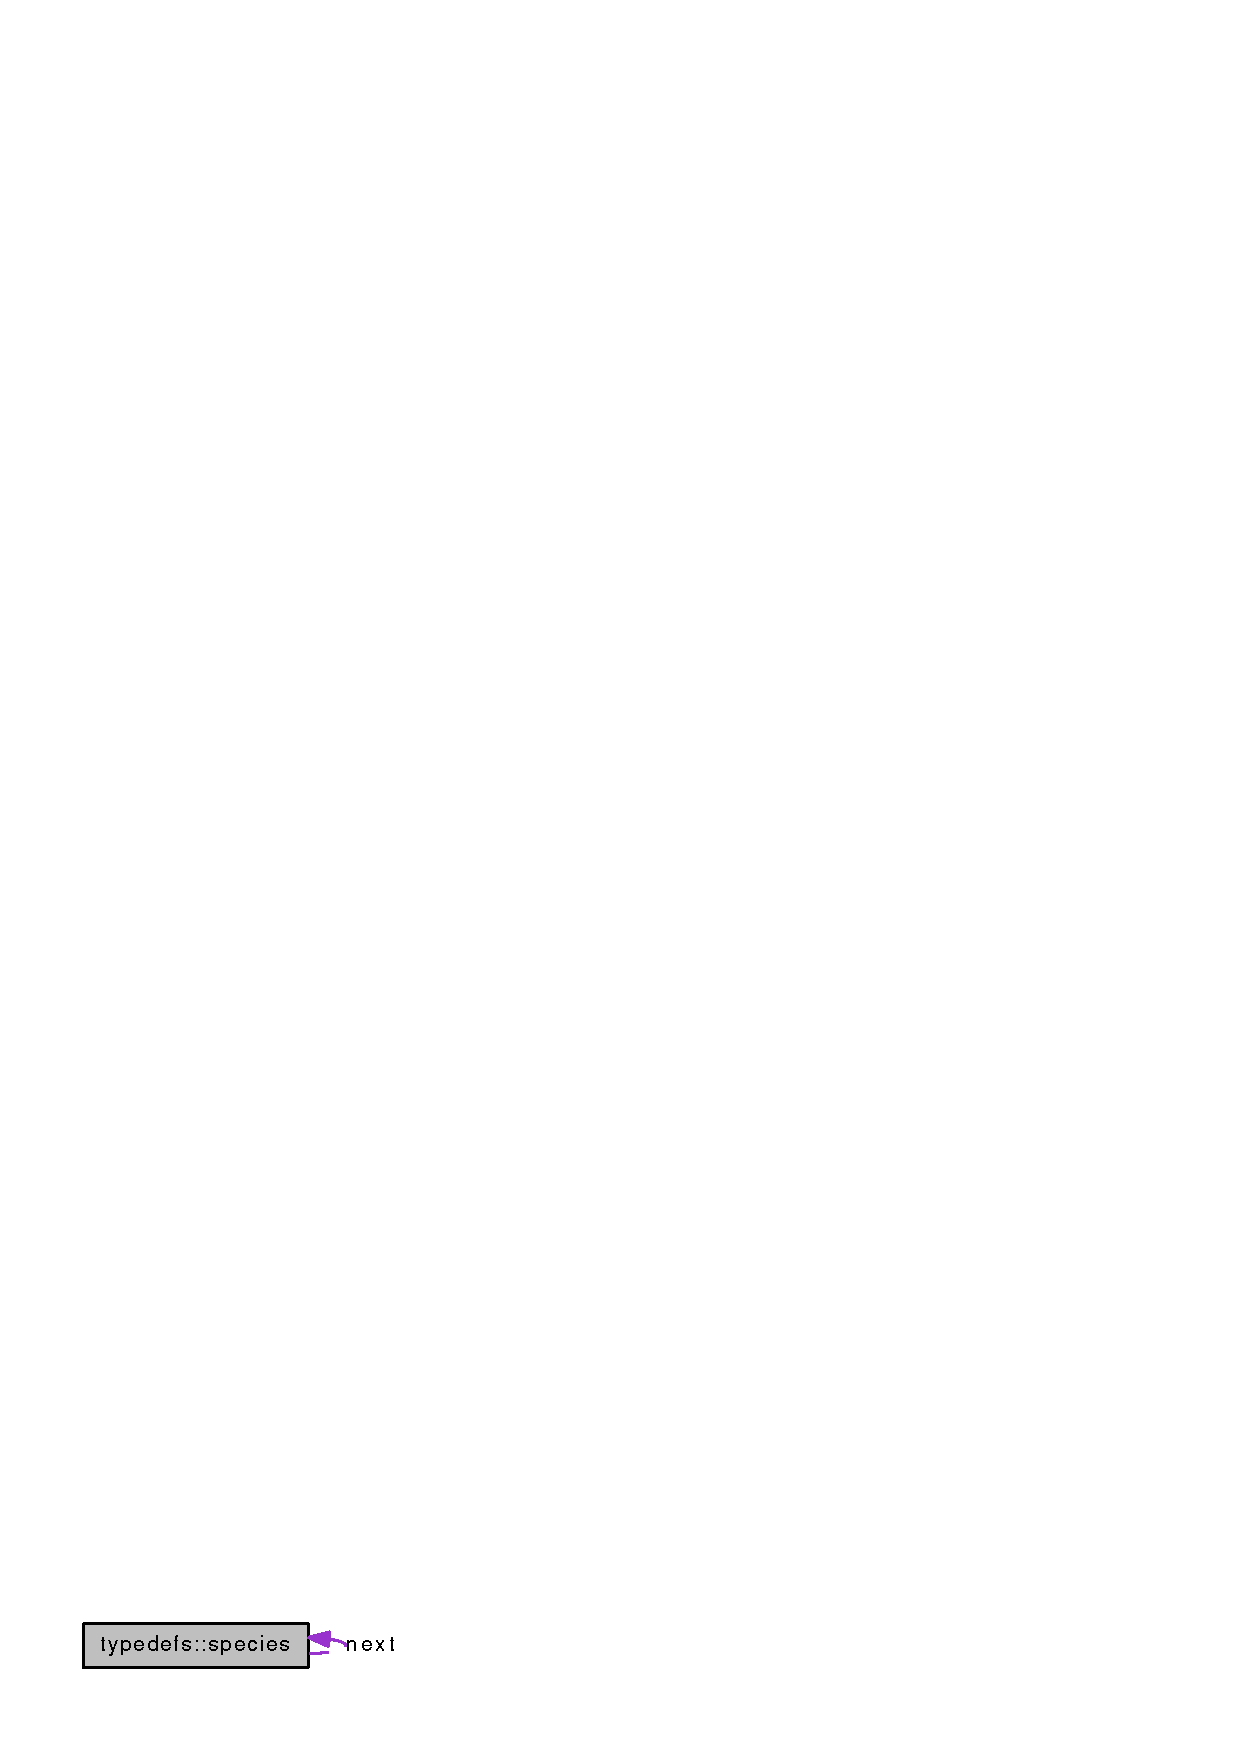
\includegraphics[width=195pt]{typetypedefs_1_1species__coll__graph}
\end{center}
\end{figure}
\subsection*{Public Attributes}
\begin{DoxyCompactItemize}
\item 
CHARACTER(len=10) \hyperlink{typetypedefs_1_1species_a381a1443f34a39b9ddee08b91fdf67b3}{name}
\item 
INTEGER \hyperlink{typetypedefs_1_1species_af824a2c036c27efd725930e6cb9c491f}{id}
\item 
integer \hyperlink{typetypedefs_1_1species_ab03f91b8ff8e8eec8c797b1514bb29b0}{atoms}
\item 
integer \hyperlink{typetypedefs_1_1species_a5dfdb92d0d495f4be8a4d957e74829a0}{charge}
\item 
DOUBLE PRECISION \hyperlink{typetypedefs_1_1species_a72f4e823e9eebde3d106419b851a5c28}{e\_\-d}
\item 
LOGICAL \hyperlink{typetypedefs_1_1species_a830e248519482ca21dc78faabcf1a798}{ion}
\item 
logical \hyperlink{typetypedefs_1_1species_a4e17d0c57396b3272a4c5f20ca437326}{exc}
\item 
LOGICAL \hyperlink{typetypedefs_1_1species_a84f8e4e86d1935d13f76a7c176f29a67}{special}
\item 
TYPE(\hyperlink{typetypedefs_1_1species}{species}), pointer \hyperlink{typetypedefs_1_1species_a8b6d25cca14915e8bd825cd6bd72265b}{next}
\end{DoxyCompactItemize}


\subsection{Detailed Description}


Definition at line 165 of file typedefs.f90.

\subsection{Member Data Documentation}
\hypertarget{typetypedefs_1_1species_ab03f91b8ff8e8eec8c797b1514bb29b0}{
\index{typedefs::species@{typedefs::species}!atoms@{atoms}}
\index{atoms@{atoms}!typedefs::species@{typedefs::species}}
\subsubsection[{atoms}]{\setlength{\rightskip}{0pt plus 5cm}integer {\bf typedefs::species::atoms}}}
\label{typetypedefs_1_1species_ab03f91b8ff8e8eec8c797b1514bb29b0}


Definition at line 168 of file typedefs.f90.\hypertarget{typetypedefs_1_1species_a5dfdb92d0d495f4be8a4d957e74829a0}{
\index{typedefs::species@{typedefs::species}!charge@{charge}}
\index{charge@{charge}!typedefs::species@{typedefs::species}}
\subsubsection[{charge}]{\setlength{\rightskip}{0pt plus 5cm}integer {\bf typedefs::species::charge}}}
\label{typetypedefs_1_1species_a5dfdb92d0d495f4be8a4d957e74829a0}


Definition at line 169 of file typedefs.f90.\hypertarget{typetypedefs_1_1species_a72f4e823e9eebde3d106419b851a5c28}{
\index{typedefs::species@{typedefs::species}!e\_\-d@{e\_\-d}}
\index{e\_\-d@{e\_\-d}!typedefs::species@{typedefs::species}}
\subsubsection[{e\_\-d}]{\setlength{\rightskip}{0pt plus 5cm}DOUBLE PRECISION {\bf typedefs::species::e\_\-d}}}
\label{typetypedefs_1_1species_a72f4e823e9eebde3d106419b851a5c28}


Definition at line 170 of file typedefs.f90.\hypertarget{typetypedefs_1_1species_a4e17d0c57396b3272a4c5f20ca437326}{
\index{typedefs::species@{typedefs::species}!exc@{exc}}
\index{exc@{exc}!typedefs::species@{typedefs::species}}
\subsubsection[{exc}]{\setlength{\rightskip}{0pt plus 5cm}logical {\bf typedefs::species::exc}}}
\label{typetypedefs_1_1species_a4e17d0c57396b3272a4c5f20ca437326}


Definition at line 172 of file typedefs.f90.\hypertarget{typetypedefs_1_1species_af824a2c036c27efd725930e6cb9c491f}{
\index{typedefs::species@{typedefs::species}!id@{id}}
\index{id@{id}!typedefs::species@{typedefs::species}}
\subsubsection[{id}]{\setlength{\rightskip}{0pt plus 5cm}INTEGER {\bf typedefs::species::id}}}
\label{typetypedefs_1_1species_af824a2c036c27efd725930e6cb9c491f}


Definition at line 167 of file typedefs.f90.\hypertarget{typetypedefs_1_1species_a830e248519482ca21dc78faabcf1a798}{
\index{typedefs::species@{typedefs::species}!ion@{ion}}
\index{ion@{ion}!typedefs::species@{typedefs::species}}
\subsubsection[{ion}]{\setlength{\rightskip}{0pt plus 5cm}LOGICAL {\bf typedefs::species::ion}}}
\label{typetypedefs_1_1species_a830e248519482ca21dc78faabcf1a798}


Definition at line 171 of file typedefs.f90.\hypertarget{typetypedefs_1_1species_a381a1443f34a39b9ddee08b91fdf67b3}{
\index{typedefs::species@{typedefs::species}!name@{name}}
\index{name@{name}!typedefs::species@{typedefs::species}}
\subsubsection[{name}]{\setlength{\rightskip}{0pt plus 5cm}CHARACTER(len=10) {\bf typedefs::species::name}}}
\label{typetypedefs_1_1species_a381a1443f34a39b9ddee08b91fdf67b3}


Definition at line 166 of file typedefs.f90.\hypertarget{typetypedefs_1_1species_a8b6d25cca14915e8bd825cd6bd72265b}{
\index{typedefs::species@{typedefs::species}!next@{next}}
\index{next@{next}!typedefs::species@{typedefs::species}}
\subsubsection[{next}]{\setlength{\rightskip}{0pt plus 5cm}TYPE({\bf species}),pointer {\bf typedefs::species::next}}}
\label{typetypedefs_1_1species_a8b6d25cca14915e8bd825cd6bd72265b}


Definition at line 174 of file typedefs.f90.\hypertarget{typetypedefs_1_1species_a84f8e4e86d1935d13f76a7c176f29a67}{
\index{typedefs::species@{typedefs::species}!special@{special}}
\index{special@{special}!typedefs::species@{typedefs::species}}
\subsubsection[{special}]{\setlength{\rightskip}{0pt plus 5cm}LOGICAL {\bf typedefs::species::special}}}
\label{typetypedefs_1_1species_a84f8e4e86d1935d13f76a7c176f29a67}


Definition at line 173 of file typedefs.f90.

The documentation for this type was generated from the following file:\begin{DoxyCompactItemize}
\item 
\hyperlink{typedefs_8f90}{typedefs.f90}\end{DoxyCompactItemize}

\hypertarget{typenewmod_1_1species}{
\section{newmod::species Type Reference}
\label{typenewmod_1_1species}\index{newmod::species@{newmod::species}}
}
Collaboration diagram for newmod::species:\nopagebreak
\begin{figure}[H]
\begin{center}
\leavevmode
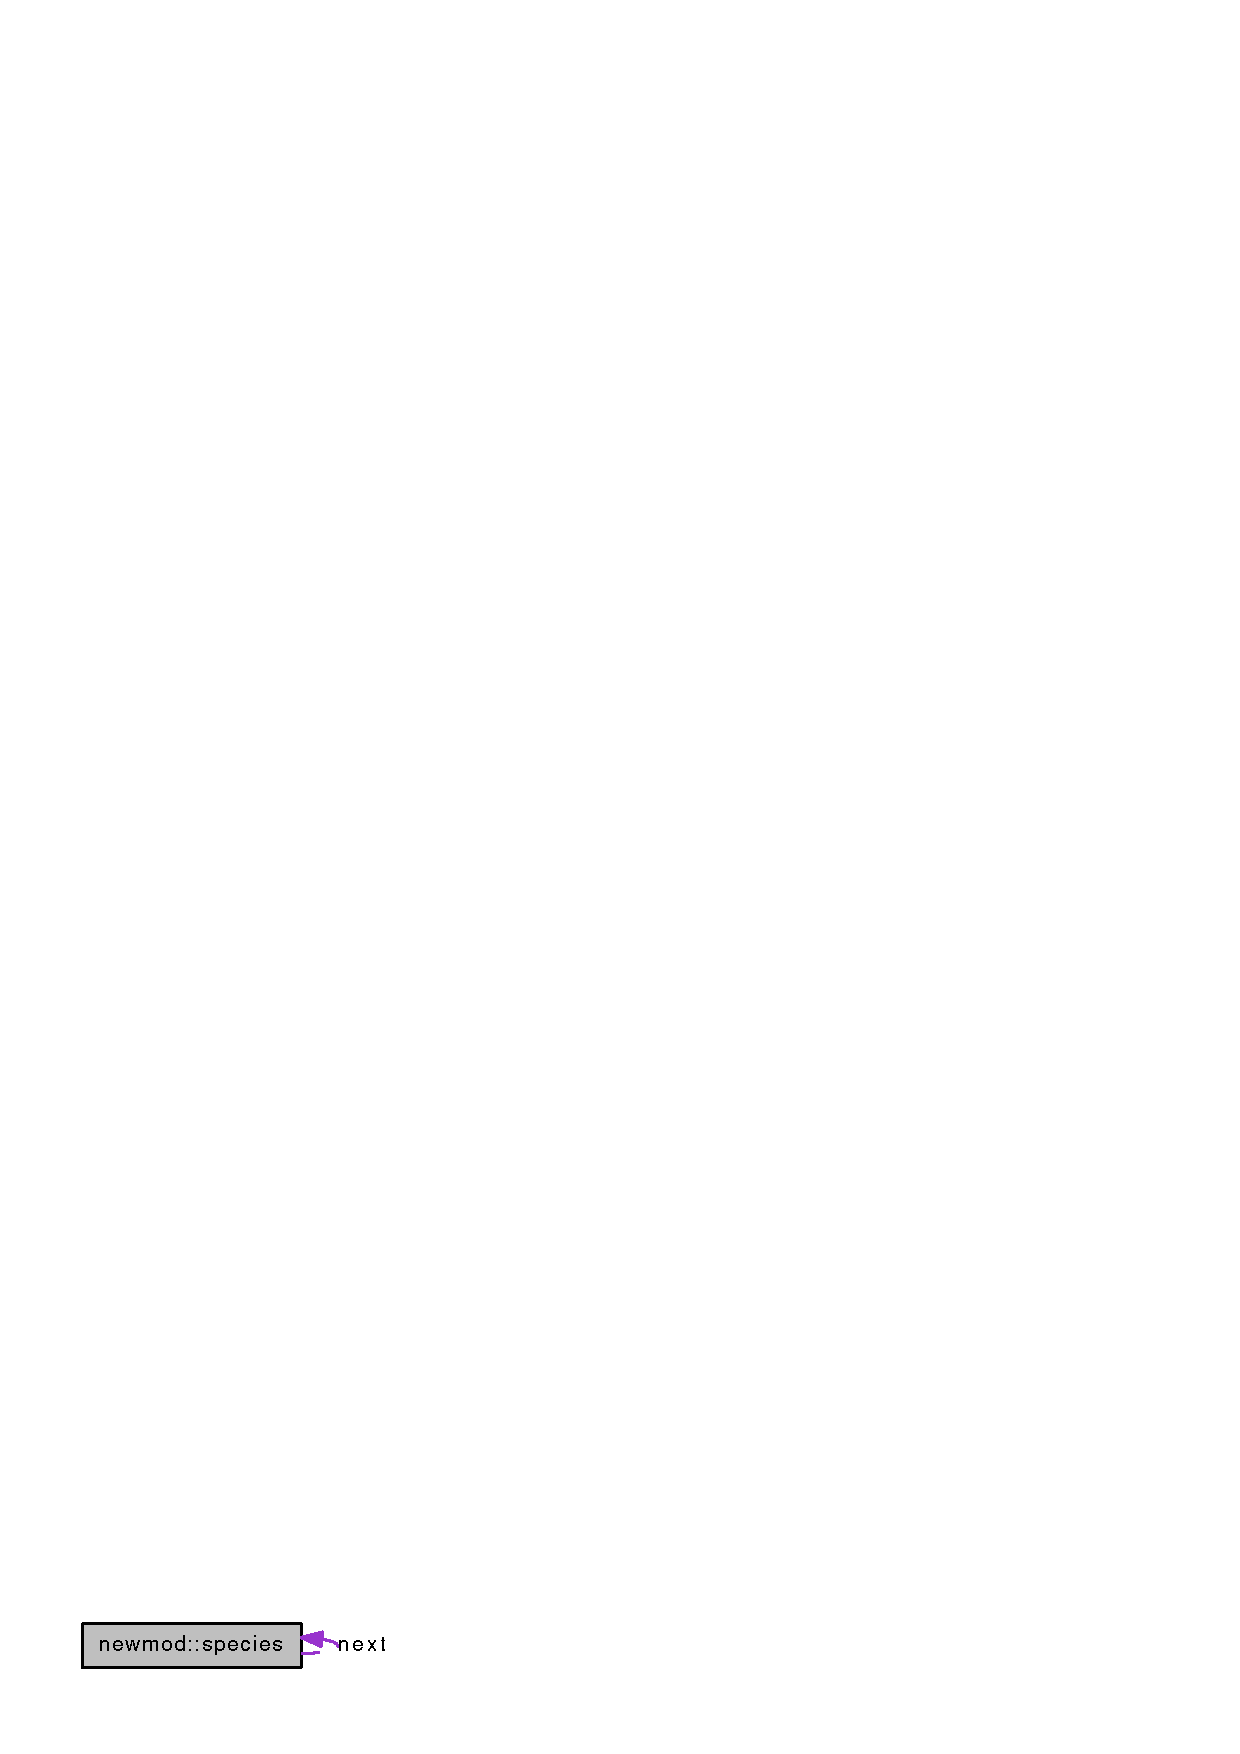
\includegraphics[width=191pt]{typenewmod_1_1species__coll__graph}
\end{center}
\end{figure}
\subsection*{Public Attributes}
\begin{DoxyCompactItemize}
\item 
CHARACTER(len=10) \hyperlink{typenewmod_1_1species_aba486adbfaa2535487376bcd1b4ae198}{name}
\item 
INTEGER \hyperlink{typenewmod_1_1species_ac55cf0b1aada54d02291ca67eb452c21}{id}
\item 
DOUBLE PRECISION \hyperlink{typenewmod_1_1species_a68e7837ef2b05186b42b3bdb318efc6d}{e\_\-d}
\item 
LOGICAL \hyperlink{typenewmod_1_1species_a4872477809d49fa74a0e59923c90098e}{ion}
\item 
LOGICAL \hyperlink{typenewmod_1_1species_ad08ea98c512c5034bb2f514fb8297dff}{special}
\item 
TYPE(\hyperlink{typenewmod_1_1species}{species}), pointer \hyperlink{typenewmod_1_1species_a17af4c156b3b9bba9284d7de99183770}{next}
\end{DoxyCompactItemize}


\subsection{Detailed Description}


Definition at line 4 of file newmod.f90.

\subsection{Member Data Documentation}
\hypertarget{typenewmod_1_1species_a68e7837ef2b05186b42b3bdb318efc6d}{
\index{newmod::species@{newmod::species}!e\_\-d@{e\_\-d}}
\index{e\_\-d@{e\_\-d}!newmod::species@{newmod::species}}
\subsubsection[{e\_\-d}]{\setlength{\rightskip}{0pt plus 5cm}DOUBLE PRECISION {\bf newmod::species::e\_\-d}}}
\label{typenewmod_1_1species_a68e7837ef2b05186b42b3bdb318efc6d}


Definition at line 7 of file newmod.f90.\hypertarget{typenewmod_1_1species_ac55cf0b1aada54d02291ca67eb452c21}{
\index{newmod::species@{newmod::species}!id@{id}}
\index{id@{id}!newmod::species@{newmod::species}}
\subsubsection[{id}]{\setlength{\rightskip}{0pt plus 5cm}INTEGER {\bf newmod::species::id}}}
\label{typenewmod_1_1species_ac55cf0b1aada54d02291ca67eb452c21}


Definition at line 6 of file newmod.f90.\hypertarget{typenewmod_1_1species_a4872477809d49fa74a0e59923c90098e}{
\index{newmod::species@{newmod::species}!ion@{ion}}
\index{ion@{ion}!newmod::species@{newmod::species}}
\subsubsection[{ion}]{\setlength{\rightskip}{0pt plus 5cm}LOGICAL {\bf newmod::species::ion}}}
\label{typenewmod_1_1species_a4872477809d49fa74a0e59923c90098e}


Definition at line 8 of file newmod.f90.\hypertarget{typenewmod_1_1species_aba486adbfaa2535487376bcd1b4ae198}{
\index{newmod::species@{newmod::species}!name@{name}}
\index{name@{name}!newmod::species@{newmod::species}}
\subsubsection[{name}]{\setlength{\rightskip}{0pt plus 5cm}CHARACTER(len=10) {\bf newmod::species::name}}}
\label{typenewmod_1_1species_aba486adbfaa2535487376bcd1b4ae198}


Definition at line 5 of file newmod.f90.\hypertarget{typenewmod_1_1species_a17af4c156b3b9bba9284d7de99183770}{
\index{newmod::species@{newmod::species}!next@{next}}
\index{next@{next}!newmod::species@{newmod::species}}
\subsubsection[{next}]{\setlength{\rightskip}{0pt plus 5cm}TYPE({\bf species}),pointer {\bf newmod::species::next}}}
\label{typenewmod_1_1species_a17af4c156b3b9bba9284d7de99183770}


Definition at line 10 of file newmod.f90.\hypertarget{typenewmod_1_1species_ad08ea98c512c5034bb2f514fb8297dff}{
\index{newmod::species@{newmod::species}!special@{special}}
\index{special@{special}!newmod::species@{newmod::species}}
\subsubsection[{special}]{\setlength{\rightskip}{0pt plus 5cm}LOGICAL {\bf newmod::species::special}}}
\label{typenewmod_1_1species_ad08ea98c512c5034bb2f514fb8297dff}


Definition at line 9 of file newmod.f90.

The documentation for this type was generated from the following file:\begin{DoxyCompactItemize}
\item 
\hyperlink{newmod_8f90}{newmod.f90}\end{DoxyCompactItemize}

\hypertarget{typetypedefs_1_1wait__info}{
\section{typedefs::wait\_\-info Type Reference}
\label{typetypedefs_1_1wait__info}\index{typedefs::wait\_\-info@{typedefs::wait\_\-info}}
}
\subsection*{Public Attributes}
\begin{DoxyCompactItemize}
\item 
DOUBLE PRECISION \hyperlink{typetypedefs_1_1wait__info_acdcf8580da31a315f32ffffad73bd9be}{wait\_\-time}
\item 
INTEGER \hyperlink{typetypedefs_1_1wait__info_a441f92d29ec79adae0f71f538b1b6f74}{i}
\item 
INTEGER \hyperlink{typetypedefs_1_1wait__info_a1752c3e6528ab490fea5c4b0928fb484}{j}
\item 
INTEGER \hyperlink{typetypedefs_1_1wait__info_a7b76d574e1f61f0167fcc70af7779329}{k}
\item 
INTEGER \hyperlink{typetypedefs_1_1wait__info_a9b6ff019fc78e04005e2dde1b603eecb}{sp\_\-num}
\item 
INTEGER \hyperlink{typetypedefs_1_1wait__info_a1c29425ab2f66b53c624cfcfe4147050}{act\_\-type}
\end{DoxyCompactItemize}


\subsection{Detailed Description}


Definition at line 3 of file typedefs.f90.

\subsection{Member Data Documentation}
\hypertarget{typetypedefs_1_1wait__info_a1c29425ab2f66b53c624cfcfe4147050}{
\index{typedefs::wait\_\-info@{typedefs::wait\_\-info}!act\_\-type@{act\_\-type}}
\index{act\_\-type@{act\_\-type}!typedefs::wait_info@{typedefs::wait\_\-info}}
\subsubsection[{act\_\-type}]{\setlength{\rightskip}{0pt plus 5cm}INTEGER {\bf typedefs::wait\_\-info::act\_\-type}}}
\label{typetypedefs_1_1wait__info_a1c29425ab2f66b53c624cfcfe4147050}


Definition at line 10 of file typedefs.f90.\hypertarget{typetypedefs_1_1wait__info_a441f92d29ec79adae0f71f538b1b6f74}{
\index{typedefs::wait\_\-info@{typedefs::wait\_\-info}!i@{i}}
\index{i@{i}!typedefs::wait_info@{typedefs::wait\_\-info}}
\subsubsection[{i}]{\setlength{\rightskip}{0pt plus 5cm}INTEGER {\bf typedefs::wait\_\-info::i}}}
\label{typetypedefs_1_1wait__info_a441f92d29ec79adae0f71f538b1b6f74}


Definition at line 8 of file typedefs.f90.\hypertarget{typetypedefs_1_1wait__info_a1752c3e6528ab490fea5c4b0928fb484}{
\index{typedefs::wait\_\-info@{typedefs::wait\_\-info}!j@{j}}
\index{j@{j}!typedefs::wait_info@{typedefs::wait\_\-info}}
\subsubsection[{j}]{\setlength{\rightskip}{0pt plus 5cm}INTEGER {\bf typedefs::wait\_\-info::j}}}
\label{typetypedefs_1_1wait__info_a1752c3e6528ab490fea5c4b0928fb484}


Definition at line 8 of file typedefs.f90.\hypertarget{typetypedefs_1_1wait__info_a7b76d574e1f61f0167fcc70af7779329}{
\index{typedefs::wait\_\-info@{typedefs::wait\_\-info}!k@{k}}
\index{k@{k}!typedefs::wait_info@{typedefs::wait\_\-info}}
\subsubsection[{k}]{\setlength{\rightskip}{0pt plus 5cm}INTEGER {\bf typedefs::wait\_\-info::k}}}
\label{typetypedefs_1_1wait__info_a7b76d574e1f61f0167fcc70af7779329}


Definition at line 8 of file typedefs.f90.\hypertarget{typetypedefs_1_1wait__info_a9b6ff019fc78e04005e2dde1b603eecb}{
\index{typedefs::wait\_\-info@{typedefs::wait\_\-info}!sp\_\-num@{sp\_\-num}}
\index{sp\_\-num@{sp\_\-num}!typedefs::wait_info@{typedefs::wait\_\-info}}
\subsubsection[{sp\_\-num}]{\setlength{\rightskip}{0pt plus 5cm}INTEGER {\bf typedefs::wait\_\-info::sp\_\-num}}}
\label{typetypedefs_1_1wait__info_a9b6ff019fc78e04005e2dde1b603eecb}


Definition at line 9 of file typedefs.f90.\hypertarget{typetypedefs_1_1wait__info_acdcf8580da31a315f32ffffad73bd9be}{
\index{typedefs::wait\_\-info@{typedefs::wait\_\-info}!wait\_\-time@{wait\_\-time}}
\index{wait\_\-time@{wait\_\-time}!typedefs::wait_info@{typedefs::wait\_\-info}}
\subsubsection[{wait\_\-time}]{\setlength{\rightskip}{0pt plus 5cm}DOUBLE PRECISION {\bf typedefs::wait\_\-info::wait\_\-time}}}
\label{typetypedefs_1_1wait__info_acdcf8580da31a315f32ffffad73bd9be}


Definition at line 7 of file typedefs.f90.

The documentation for this type was generated from the following file:\begin{DoxyCompactItemize}
\item 
\hyperlink{typedefs_8f90}{typedefs.f90}\end{DoxyCompactItemize}

\chapter{File Documentation}
\hypertarget{branchmod_8f90}{
\section{branchmod.f90 File Reference}
\label{branchmod_8f90}\index{branchmod.f90@{branchmod.f90}}
}
\subsection*{Modules}
\begin{DoxyCompactItemize}
\item 
module \hyperlink{namespacebranchmod}{branchmod}
\end{DoxyCompactItemize}
\subsection*{Functions/Subroutines}
\begin{DoxyCompactItemize}
\item 
INTEGER \hyperlink{namespacebranchmod_afe047e9cf349dd7beea43ce0113ab24b}{branchmod::branching} (reactant1, reactant2, pr)
\item 
subroutine \hyperlink{namespacebranchmod_a37435a321ae1297821d708a3891bdf0d}{branchmod::bumpreaction} (id, \hyperlink{typetypedefs_1_1node}{node})
\item 
subroutine \hyperlink{namespacebranchmod_a4c2d31e67892bffa2413995834db274a}{branchmod::selectbranch} (kvals, ndex)
\end{DoxyCompactItemize}

\hypertarget{bresenham_8f90}{
\section{bresenham.f90 File Reference}
\label{bresenham_8f90}\index{bresenham.f90@{bresenham.f90}}
}
\subsection*{Functions/Subroutines}
\begin{DoxyCompactItemize}
\item 
subroutine \hyperlink{bresenham_8f90_ab47b475845f9c900058b13a8f016ea92}{bresenham} (x1, y1, x2, y2)
\end{DoxyCompactItemize}


\subsection{Function Documentation}
\hypertarget{bresenham_8f90_ab47b475845f9c900058b13a8f016ea92}{
\index{bresenham.f90@{bresenham.f90}!bresenham@{bresenham}}
\index{bresenham@{bresenham}!bresenham.f90@{bresenham.f90}}
\subsubsection[{bresenham}]{\setlength{\rightskip}{0pt plus 5cm}subroutine bresenham (INTEGER,intent(in) {\em x1}, \/  INTEGER,intent(in) {\em y1}, \/  INTEGER,intent(in) {\em x2}, \/  INTEGER,intent(in) {\em y2})}}
\label{bresenham_8f90_ab47b475845f9c900058b13a8f016ea92}


Definition at line 4 of file bresenham.f90.
\hypertarget{bsimple_8f90}{
\section{bsimple.f90 File Reference}
\label{bsimple_8f90}\index{bsimple.f90@{bsimple.f90}}
}
\subsection*{Data Types}
\begin{DoxyCompactItemize}
\item 
interface \hyperlink{interfacebsimple_1_1OPERATOR_07_4_08}{bsimple::OPERATOR($>$)}
\item 
interface {\bfseries bsimple::OPERATOR($<$)}
\item 
interface {\bfseries bsimple::OPERATOR(==)}
\end{DoxyCompactItemize}
\subsection*{Modules}
\begin{DoxyCompactItemize}
\item 
module \hyperlink{namespacebsimple}{bsimple}
\end{DoxyCompactItemize}
\subsection*{Functions/Subroutines}
\begin{DoxyCompactItemize}
\item 
subroutine \hyperlink{namespacebsimple_a98a0fa9db2215d588a0a87c08065809f}{bsimple::add\_\-node} (ptr, new\_\-node)
\item 
subroutine \hyperlink{namespacebsimple_ae6c8fc172ff255d4d825b1f507d9fd82}{bsimple::write\_\-node} (ptr)
\item 
subroutine \hyperlink{namespacebsimple_abe5b608758a905e30ed8661e177395d6}{bsimple::find\_\-node} (ptr, search, error)
\item 
subroutine \hyperlink{namespacebsimple_a021b297f11aa3649405b7931d0979be9}{bsimple::find\_\-previous} (ptr, search, prevNode, leftRight, error)
\item 
subroutine \hyperlink{namespacebsimple_a11b24c82d3405b40e38891f5b2de1eeb}{bsimple::find\_\-min} (ptr, search)
\item 
subroutine \hyperlink{namespacebsimple_a4cb5aa13e4c5a527c7573ccbd5234162}{bsimple::delete\_\-node} (root, toDelete, prevNode, nextNode, error)
\end{DoxyCompactItemize}

\hypertarget{functiondefs_8f90}{
\section{functiondefs.f90 File Reference}
\label{functiondefs_8f90}\index{functiondefs.f90@{functiondefs.f90}}
}
\subsection*{Modules}
\begin{DoxyCompactItemize}
\item 
module \hyperlink{namespacefunctiondefs}{functiondefs}
\end{DoxyCompactItemize}
\subsection*{Functions/Subroutines}
\begin{DoxyCompactItemize}
\item 
DOUBLE PRECISION \hyperlink{namespacefunctiondefs_ae9b1c95ccb465d122918ab89da45aed7}{functiondefs::arrhenius} (a, b, c)
\item 
DOUBLE PRECISION \hyperlink{namespacefunctiondefs_ad75756612cb12ba4983414cdc520f6a1}{functiondefs::green\_\-mcneal} (energy, a, j, nu, omega, z, i)
\item 
DOUBLE PRECISION \hyperlink{namespacefunctiondefs_a9cd4ed9f980bd43386e7de1e3e35c79c}{functiondefs::a\_\-gs} (energy, k, k\_\-b, j, j\_\-b, j\_\-c)
\item 
DOUBLE PRECISION \hyperlink{namespacefunctiondefs_adae12a3980d4e2bd5fe6277c91988474}{functiondefs::gamma\_\-gs} (energy, gamma\_\-s, gamma\_\-b)
\item 
DOUBLE PRECISION \hyperlink{namespacefunctiondefs_a5e1c4c25a7352f149e1f18854c37930f}{functiondefs::t\_\-0\_\-gs} (energy, t\_\-a, t\_\-b, t\_\-s)
\item 
DOUBLE PRECISION \hyperlink{namespacefunctiondefs_a7beb6f6af6e15afda97da88dde407655}{functiondefs::t\_\-max\_\-gs} (energy, i)
\item 
DOUBLE PRECISION \hyperlink{namespacefunctiondefs_a64cc5970914d70f20e127be3722f11bb}{functiondefs::green\_\-sawada} (a, gamma\_\-fac, t\_\-max, t\_\-0)
\item 
REAL \hyperlink{namespacefunctiondefs_abb5f2d51b3f8b637e0d17ad8c21db948}{functiondefs::ne\_\-mg} (gamma\_\-fac, t\_\-max, t\_\-0)
\item 
subroutine \hyperlink{namespacefunctiondefs_a93c18b11591055e1e1275c6dc7b2ab26}{functiondefs::magic} (eps, b, c2, s2, theta)
\item 
DOUBLE PRECISION \hyperlink{namespacefunctiondefs_a34160b04b7880953967f273645a835c5}{functiondefs::b\_\-magic} (rn, a, rho)
\item 
DOUBLE PRECISION \hyperlink{namespacefunctiondefs_abf4df469161d4f4092a1a538a20ebf1d}{functiondefs::au} (z1, z2)
\item 
DOUBLE PRECISION \hyperlink{namespacefunctiondefs_ac20c2b09d0408eb23b226af7f8f7361a}{functiondefs::eps} (en, z1, z2, m1, m2, au)
\item 
DOUBLE PRECISION \hyperlink{namespacefunctiondefs_aa92057c8da0a7ce374166fed435ea54f}{functiondefs::mass\_\-fac} (m1, m2)
\item 
DOUBLE PRECISION \hyperlink{namespacefunctiondefs_a529a6bcbb0305c32f0275aa85d4303e8}{functiondefs::t\_\-coll} (e, mf, s2)
\item 
DOUBLE PRECISION \hyperlink{namespacefunctiondefs_abeba54805575687a8d1db47decf4790e}{functiondefs::lab\_\-theta} (cmtheta, m1, m2)
\item 
DOUBLE PRECISION \hyperlink{namespacefunctiondefs_a80d99fe52a1cb5856694596955d8aeb9}{functiondefs::sneps} (eps)
\item 
DOUBLE PRECISION \hyperlink{namespacefunctiondefs_a78455979576075ad68feb125604462bc}{functiondefs::sne} (sneps, z1, z2, m1, m2)
\item 
DOUBLE PRECISION \hyperlink{namespacefunctiondefs_ae52b03b9e83dd8f46fd7532fb105850b}{functiondefs::pelsig} (energy, sne, mf)
\item 
DOUBLE PRECISION \hyperlink{namespacefunctiondefs_a7a31d88fad502937338eafac9a574fec}{functiondefs::greendutta} (energy, w, f, o, a, b)
\item 
DOUBLE PRECISION \hyperlink{namespacefunctiondefs_a5486e5e48a1c871c2ec9d5bc03406ea5}{functiondefs::pjgsigma} (energy, f, w, c, a, b)
\end{DoxyCompactItemize}

\hypertarget{gp_8f90}{
\section{gp.f90 File Reference}
\label{gp_8f90}\index{gp.f90@{gp.f90}}
}
\subsection*{Modules}
\begin{DoxyCompactItemize}
\item 
module \hyperlink{namespacegp}{gp}
\end{DoxyCompactItemize}
\subsection*{Functions/Subroutines}
\begin{DoxyCompactItemize}
\item 
subroutine \hyperlink{namespacegp_a0b4ea7e3d8474c9cb6eabeb9581a28b2}{gp::fitness} (unfit, total\_\-fitness)
\item 
subroutine \hyperlink{namespacegp_acef1117d5406847ad3fab8456f70bad7}{gp::store\_\-rand} ()
\end{DoxyCompactItemize}

\hypertarget{main_8f90}{
\section{main.f90 File Reference}
\label{main_8f90}\index{main.f90@{main.f90}}
}
\subsection*{Functions/Subroutines}
\begin{DoxyCompactItemize}
\item 
program \hyperlink{main_8f90_a8ec2266d83cd6c0b762cbcbc92c0af3d}{main}
\end{DoxyCompactItemize}


\subsection{Function Documentation}
\hypertarget{main_8f90_a8ec2266d83cd6c0b762cbcbc92c0af3d}{
\index{main.f90@{main.f90}!main@{main}}
\index{main@{main}!main.f90@{main.f90}}
\subsubsection[{main}]{\setlength{\rightskip}{0pt plus 5cm}program main ()}}
\label{main_8f90_a8ec2266d83cd6c0b762cbcbc92c0af3d}


Definition at line 1 of file main.f90.

References parameters::AB\_\-LUN, bsimple::add\_\-node(), parameters::AREA, readinput::buildnetwork(), parameters::COUNT\_\-COUNT, subroutines::counter(), parameters::CRPNUM, parameters::DEBUG, bsimple::delete\_\-node(), parameters::DIMENS, parameters::E\_\-BULK, parameters::ELECNUM, parameters::EN\_\-LIST, parameters::EXCNUM, subroutines::fallout(), parameters::fast\_\-reacts, bsimple::find\_\-min(), gp::fitness(), parameters::FIX1, parameters::FIX2, parameters::FIX3, parameters::FIX\_\-FREQ, parameters::FIXED\_\-SIZE, parameters::FLUENCE, parameters::FLUENCE\_\-TOTAL, parameters::GEMINACY\_\-FILE, parameters::GEMINACY\_\-LUN, subroutines::hopping(), subroutines::init\_\-node(), parameters::initialatoms, parameters::MATRIX, parameters::MNUM, parameters::N\_\-O3HOP, parameters::N\_\-OHOP, parameters::NEDGE, subroutines::new\_\-reaction(), parameters::NTHICK, parameters::NUM\_\-SPECIES, parameters::NUMPROTONS, parameters::O2\_\-ABUNDANCE, parameters::O3\_\-ABUNDANCE, parameters::O3\_\-ANALYTICS, parameters::O3NUM, parameters::O\_\-ABUNDANCE, parameters::ONUM, parameters::PROTON\_\-COLL, parameters::PROTON\_\-ELOSS, parameters::RATE\_\-LUN, parameters::RATEINFO, parameters::TIME, parameters::TIME\_\-FREQ, parameters::TOTAL\_\-PROTON\_\-ELOSS, parameters::TRACK\_\-AN\_\-LUN, subroutines::wait\_\-calc(), and subroutines::wipe\_\-node().

Here is the call graph for this function:\nopagebreak
\begin{figure}[H]
\begin{center}
\leavevmode
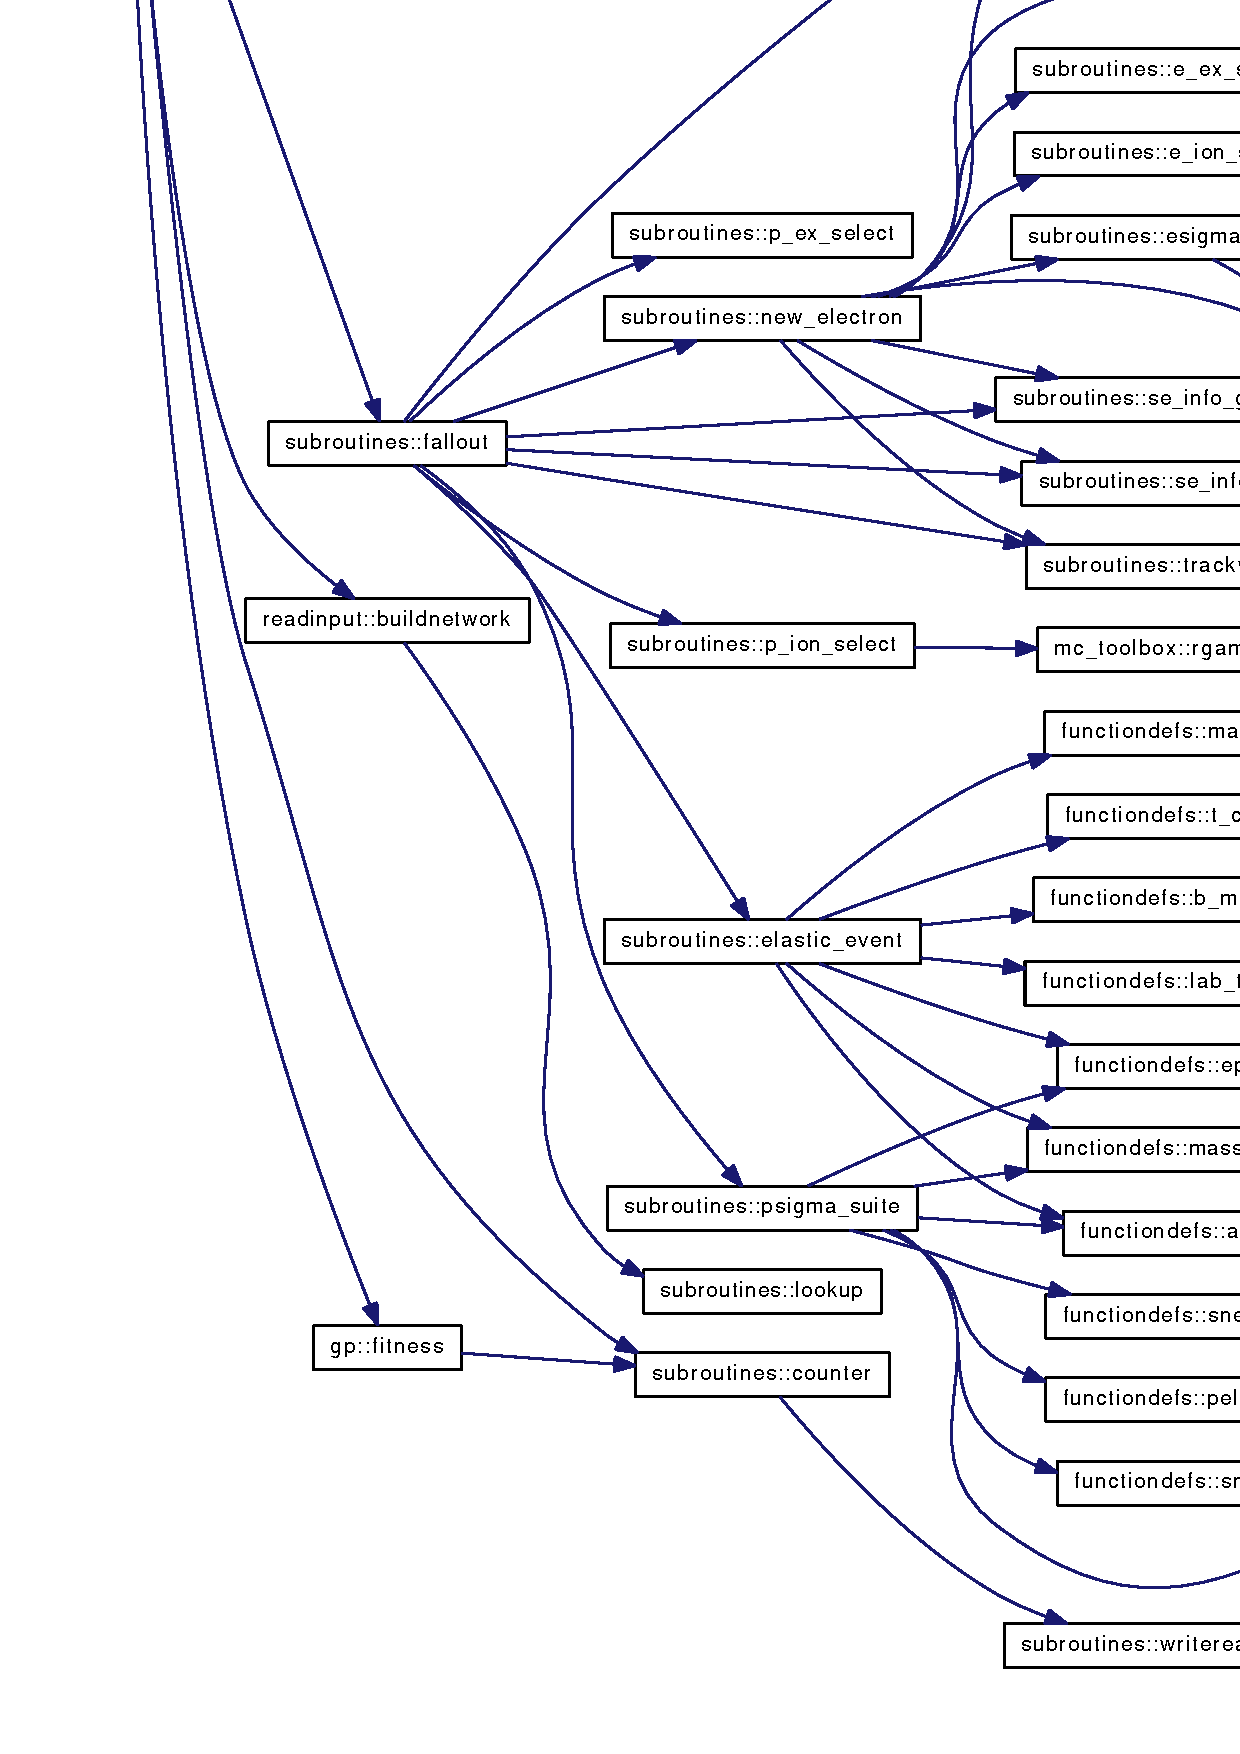
\includegraphics[width=420pt]{main_8f90_a8ec2266d83cd6c0b762cbcbc92c0af3d_cgraph}
\end{center}
\end{figure}

\hypertarget{mc__toolbox_8f90}{
\section{mc\_\-toolbox.f90 File Reference}
\label{mc__toolbox_8f90}\index{mc\_\-toolbox.f90@{mc\_\-toolbox.f90}}
}
\subsection*{Modules}
\begin{DoxyCompactItemize}
\item 
module \hyperlink{namespacemc__toolbox}{mc\_\-toolbox}
\end{DoxyCompactItemize}
\subsection*{Functions/Subroutines}
\begin{DoxyCompactItemize}
\item 
REAL(KIND=8) \hyperlink{namespacemc__toolbox_acedafdf57f1c1cd3610359fe837a708d}{mc\_\-toolbox::rgamma} (a)
\item 
real(kind=8) \hyperlink{namespacemc__toolbox_ab8fa538b6e1b30d65864f793e75425ea}{mc\_\-toolbox::r8\_\-normal\_\-01} ()
\item 
real(kind=8) \hyperlink{namespacemc__toolbox_a405cb2a6c8bceb2f89fc0da987cd399a}{mc\_\-toolbox::r8\_\-uniform\_\-01} (seedy)
\item 
real(kind=8) \hyperlink{namespacemc__toolbox_aab33e2e1a35352d1550e81fb86fb1cc9}{mc\_\-toolbox::r8\_\-normal\_\-ab} (a, b)
\end{DoxyCompactItemize}
\subsection*{Variables}
\begin{DoxyCompactItemize}
\item 
INTEGER(KIND=4), parameter \hyperlink{namespacemc__toolbox_a2b3c4edff260f415453579697b0a5282}{mc\_\-toolbox::GSEED} = 12345
\item 
REAL(KIND=8), parameter \hyperlink{namespacemc__toolbox_a9e72a666484c36244e37a8083e792dd8}{mc\_\-toolbox::MEANVAL} = 0.00
\item 
REAL(KIND=8), parameter \hyperlink{namespacemc__toolbox_a5655149a57d9d21f98b7515536fe1a1b}{mc\_\-toolbox::SDEV} = 2.00
\end{DoxyCompactItemize}

\hypertarget{newbranch_8f90}{
\section{newbranch.f90 File Reference}
\label{newbranch_8f90}\index{newbranch.f90@{newbranch.f90}}
}
\subsection*{Modules}
\begin{DoxyCompactItemize}
\item 
module \hyperlink{namespacebranchmod}{branchmod}
\end{DoxyCompactItemize}
\subsection*{Functions/Subroutines}
\begin{DoxyCompactItemize}
\item 
INTEGER \hyperlink{namespacebranchmod_afe047e9cf349dd7beea43ce0113ab24b}{branchmod::branching} (reactant1, reactant2, pr)
\end{DoxyCompactItemize}

\hypertarget{newmod_8f90}{
\section{newmod.f90 File Reference}
\label{newmod_8f90}\index{newmod.f90@{newmod.f90}}
}
\subsection*{Data Types}
\begin{DoxyCompactItemize}
\item 
type \hyperlink{typenewmod_1_1species}{newmod::species}
\item 
type \hyperlink{typenewmod_1_1reaction}{newmod::reaction}
\end{DoxyCompactItemize}
\subsection*{Modules}
\begin{DoxyCompactItemize}
\item 
module \hyperlink{namespacenewmod}{newmod}
\end{DoxyCompactItemize}
\subsection*{Functions/Subroutines}
\begin{DoxyCompactItemize}
\item 
subroutine \hyperlink{namespacenewmod_a6e08d1c91ffcb8d044e3ad8d8b535348}{newmod::lookup} (name, node, id)
\end{DoxyCompactItemize}

\hypertarget{newnet_8f90}{
\section{newnet.f90 File Reference}
\label{newnet_8f90}\index{newnet.f90@{newnet.f90}}
}
\subsection*{Functions/Subroutines}
\begin{DoxyCompactItemize}
\item 
program \hyperlink{newnet_8f90_ab35c702ef6e4d765bfb3073f91892007}{newnet}
\end{DoxyCompactItemize}


\subsection{Function Documentation}
\hypertarget{newnet_8f90_ab35c702ef6e4d765bfb3073f91892007}{
\index{newnet.f90@{newnet.f90}!newnet@{newnet}}
\index{newnet@{newnet}!newnet.f90@{newnet.f90}}
\subsubsection[{newnet}]{\setlength{\rightskip}{0pt plus 5cm}program newnet ()}}
\label{newnet_8f90_ab35c702ef6e4d765bfb3073f91892007}


Definition at line 1 of file newnet.f90.

References newmod::lookup().

Here is the call graph for this function:\nopagebreak
\begin{figure}[H]
\begin{center}
\leavevmode
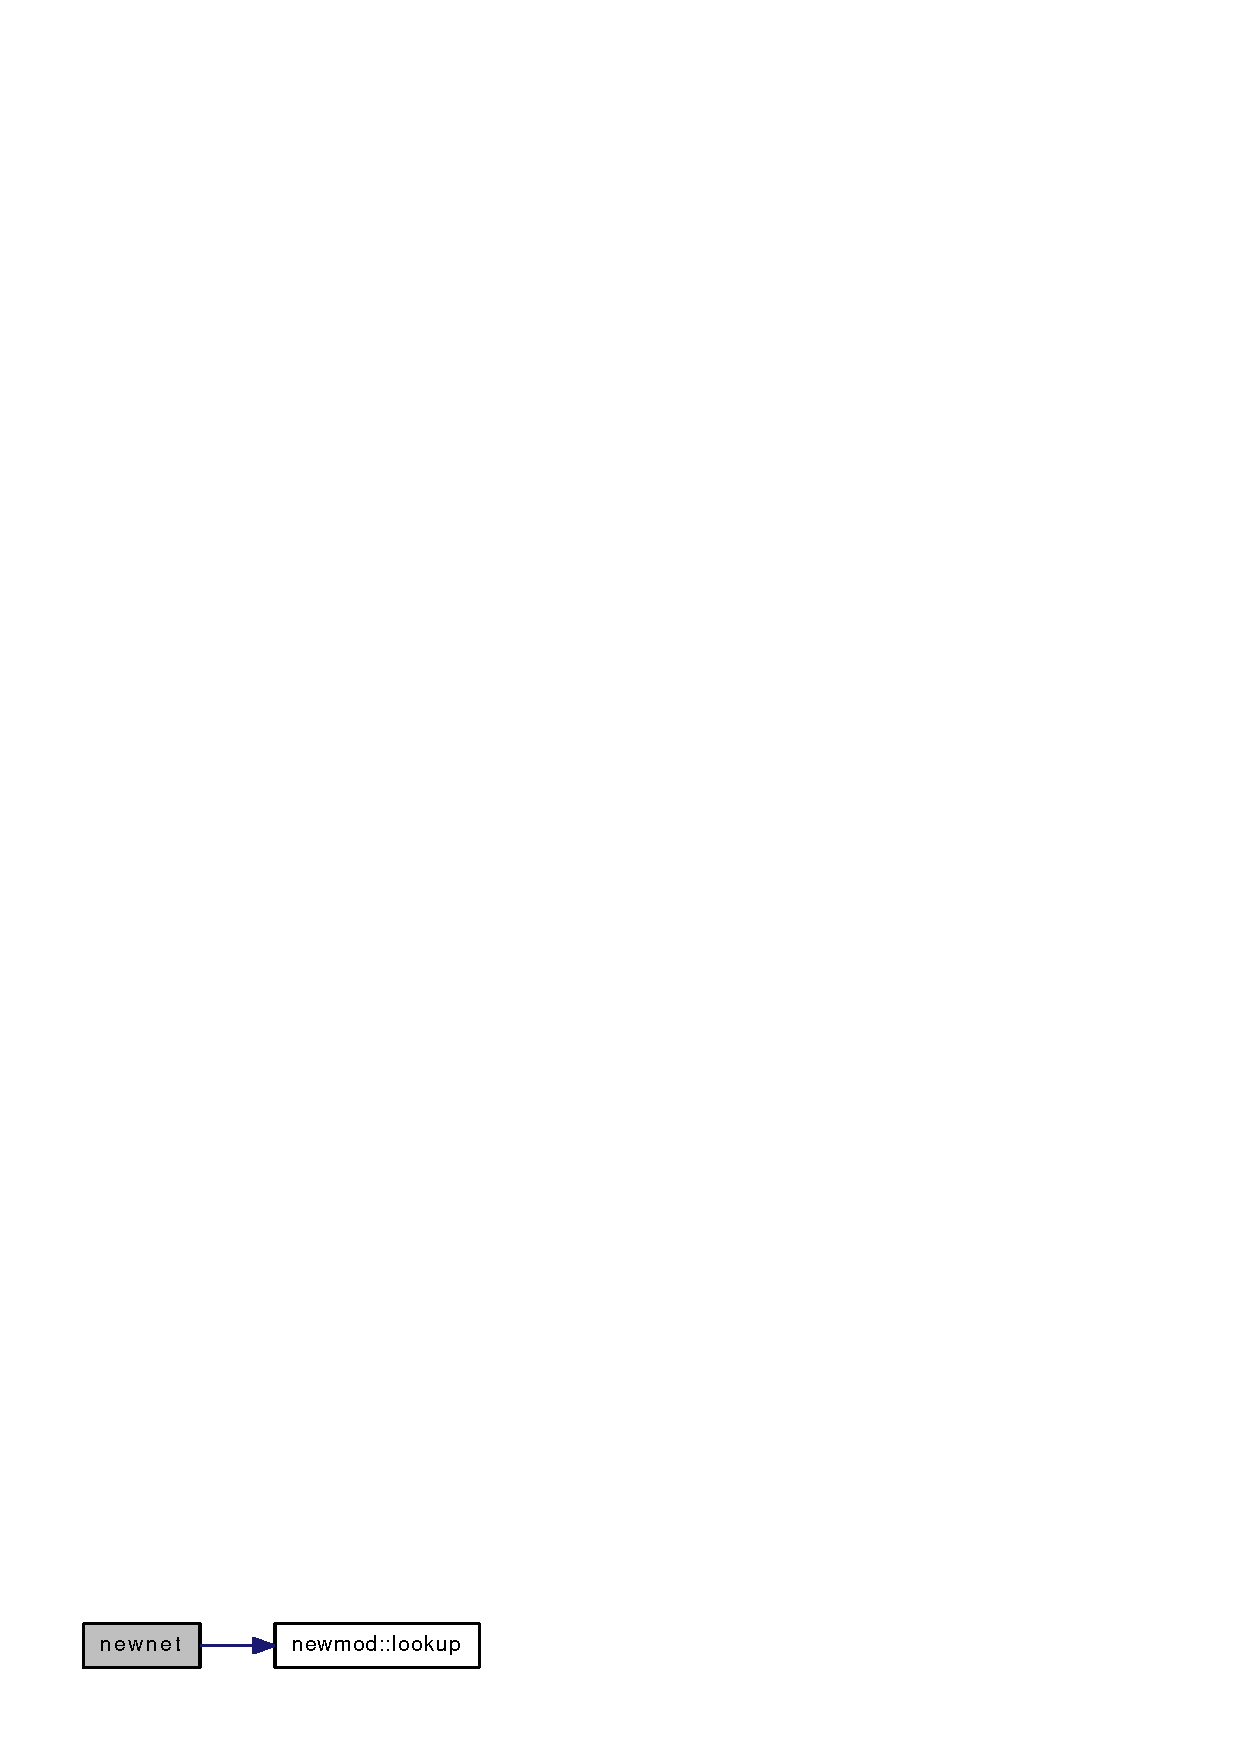
\includegraphics[width=117pt]{newnet_8f90_ab35c702ef6e4d765bfb3073f91892007_cgraph}
\end{center}
\end{figure}

\hypertarget{old__branchmod_8f90}{
\section{old\_\-branchmod.f90 File Reference}
\label{old__branchmod_8f90}\index{old\_\-branchmod.f90@{old\_\-branchmod.f90}}
}
\subsection*{Modules}
\begin{DoxyCompactItemize}
\item 
module \hyperlink{namespacebranchmod}{branchmod}
\end{DoxyCompactItemize}
\subsection*{Functions/Subroutines}
\begin{DoxyCompactItemize}
\item 
INTEGER \hyperlink{namespacebranchmod_afe047e9cf349dd7beea43ce0113ab24b}{branchmod::branching} (reactant1, reactant2, pr)
\end{DoxyCompactItemize}

\hypertarget{parameters_8f90}{
\section{parameters.f90 File Reference}
\label{parameters_8f90}\index{parameters.f90@{parameters.f90}}
}
\subsection*{Modules}
\begin{DoxyCompactItemize}
\item 
module \hyperlink{namespaceparameters}{parameters}
\end{DoxyCompactItemize}
\subsection*{Variables}
\begin{DoxyCompactItemize}
\item 
TYPE(node), allocatable, target \hyperlink{namespaceparameters_a1d2ec6532bce135a8fc18f3542969a8d}{parameters::MATRIX}
\item 
INTEGER \hyperlink{namespaceparameters_a8eba14af35a7a362f50093f1acc28a78}{parameters::DIMENS}
\item 
INTEGER \hyperlink{namespaceparameters_a00c44079184906f8aff60ad7cea2fe4d}{parameters::PRODS}
\item 
DOUBLE PRECISION, allocatable \hyperlink{namespaceparameters_a41b06e1dd582bb56419bf991f2c633e3}{parameters::EN\_\-LIST}
\item 
CHARACTER(LEN=10), allocatable \hyperlink{namespaceparameters_a38878c1dc241cdcfc52f1804563f7b00}{parameters::SP\_\-LIST}
\item 
INTEGER, allocatable \hyperlink{namespaceparameters_a660ab08d014ed8f467dc504ed8585591}{parameters::IONLIST}
\item 
INTEGER, allocatable \hyperlink{namespaceparameters_a649c343c05b95e3f84d06401b3a3f6e1}{parameters::SP\_\-PROD\_\-DEST}
\item 
integer, dimension(:), allocatable \hyperlink{namespaceparameters_a8706bba63c5517e5b5e5b2cf0487db4b}{parameters::fast\_\-reacts}
\item 
INTEGER \hyperlink{namespaceparameters_aed3ebeff9daeb47edfa593ae2b72d4db}{parameters::NUM\_\-SPECIES} = 0
\item 
INTEGER \hyperlink{namespaceparameters_a1462d3a8d5ef4ee00ffc9c0beac695b2}{parameters::NUM\_\-REACTS} = 0
\item 
INTEGER \hyperlink{namespaceparameters_abf21c9c60fbc062ca9e84d2746c7388a}{parameters::NUMPROTONS} = 0
\item 
DOUBLE PRECISION \hyperlink{namespaceparameters_acf1d338d691bf2082aeabaec6ac27263}{parameters::TIME} = 0
\item 
TYPE(reaction), pointer \hyperlink{namespaceparameters_aff68a046aeb1fa2a7610db8cd55922d8}{parameters::RE\_\-HEAD}
\item 
integer \hyperlink{namespaceparameters_a2a130bb0e6ad790a2a783d19749cc8ce}{parameters::initialatoms} = 0
\item 
REAL \hyperlink{namespaceparameters_a3c39b69e0083dc018e4546bd5a02b301}{parameters::GVALUE} = 0
\item 
REAL \hyperlink{namespaceparameters_a2855e0778fdd644c62b1a6943a4c363a}{parameters::CUIRCT} = 0
\item 
REAL \hyperlink{namespaceparameters_a170cb61fd1eef5175a5eaf95d0d85ab5}{parameters::CUPREL} = 0
\item 
INTEGER \hyperlink{namespaceparameters_a38fbcf3f41331f232ff4c604194bc76f}{parameters::PMODEL} = 0
\item 
CHARACTER(LEN=80), parameter \hyperlink{namespaceparameters_af23a39fc248303c9a69e3e05c0fb3b41}{parameters::SPECIES\_\-FILE}
\item 
CHARACTER(LEN=80), parameter \hyperlink{namespaceparameters_a40ef599fa2e91d0f27cbd322f1270da8}{parameters::REACTIONS\_\-FILE}
\item 
CHARACTER(LEN=80), parameter \hyperlink{namespaceparameters_adf79c33c6ebf2e4f00fa0fdaf34d1ba1}{parameters::PARAMS\_\-FILE}
\item 
CHARACTER(LEN=80), parameter \hyperlink{namespaceparameters_a045269697aa491915bf603f55e12b63a}{parameters::GEMINACY\_\-FILE}
\item 
DOUBLE PRECISION, parameter \hyperlink{namespaceparameters_a5f4fb781d85daf37e0a18e15e4dcc9c8}{parameters::EINIT} = 100D3
\item 
DOUBLE PRECISION, parameter \hyperlink{namespaceparameters_a1f6362692e1384b097b58b185096b416}{parameters::CDIM} = 3.414e-\/8
\item 
DOUBLE PRECISION, parameter \hyperlink{namespaceparameters_a3a667857cb5e332f397b7ff0e96dbb85}{parameters::BDIM} = 6.668e-\/8
\item 
DOUBLE PRECISION, parameter \hyperlink{namespaceparameters_ad2ed15127be0caca99788b8acc6e605b}{parameters::ADIM} = 9.225e-\/8
\item 
DOUBLE PRECISION, parameter \hyperlink{namespaceparameters_aaa3c163a9f90b6d0c5a314ca449da18b}{parameters::BETACRYS} = 85.05
\item 
DOUBLE PRECISION, parameter \hyperlink{namespaceparameters_a998d2db873404e0cfe943d50d3877262}{parameters::C\_\-PR} = CDIM$\ast$COS(90-\/BETACRYS)
\item 
DOUBLE PRECISION, parameter \hyperlink{namespaceparameters_ad8323286536365bb131984aa57af99df}{parameters::RHO} = 1.313E22
\item 
DOUBLE PRECISION, parameter \hyperlink{namespaceparameters_a79fa48b917f68e1a12577e33fd8c991c}{parameters::RHO2} = 0.01313
\item 
INTEGER, parameter \hyperlink{namespaceparameters_a2fbeb743f79ed8a1c34482eb24ce3e87}{parameters::FIX1} = 150
\item 
INTEGER, parameter \hyperlink{namespaceparameters_a11cddb5a155baade8a969acb80c17292}{parameters::FIX2} = 150
\item 
INTEGER, parameter \hyperlink{namespaceparameters_adedf5e0e6373ffbf611e8767d9cf0e80}{parameters::FIX3} = 150
\item 
DOUBLE PRECISION, parameter \hyperlink{namespaceparameters_aacbd355b27d7e7459076fdf3f77fab20}{parameters::THICK} = 1.0e-\/5
\item 
DOUBLE PRECISION, parameter \hyperlink{namespaceparameters_a45377074e21edf9bd71351430490cd5e}{parameters::EDGE} = 3.5e-\/6
\item 
DOUBLE PRECISION, parameter \hyperlink{namespaceparameters_a8a887d07bb62f10ae5578c2a7181a578}{parameters::VOLUME} = THICK$\ast$EDGE$\ast$EDGE
\item 
DOUBLE PRECISION, parameter \hyperlink{namespaceparameters_a144dd87a3ad4a40138cad0b8d26ee282}{parameters::KIN\_\-TEMP} = 5.0D0
\item 
DOUBLE PRECISION, parameter \hyperlink{namespaceparameters_aee8d50a231f8beed7edc0ff5ba2437f4}{parameters::AREA} = EDGE$\ast$EDGE
\item 
DOUBLE PRECISION, parameter \hyperlink{namespaceparameters_ad9a62be82a2fb56fe291f73d3279d4b4}{parameters::CR\_\-FLUX} = 1.0D11
\item 
DOUBLE PRECISION, parameter \hyperlink{namespaceparameters_ac433c7adc61bc138dfc7567a570833ed}{parameters::CR\_\-RATE} = CR\_\-FLUX$\ast$AREA
\item 
DOUBLE PRECISION, parameter \hyperlink{namespaceparameters_a20c80b2e34c240feef7ac6887646115d}{parameters::NELEM} = 3.0$\ast$RHO$\ast$(THICK$\ast$EDGE$\ast$EDGE)
\item 
DOUBLE PRECISION, parameter \hyperlink{namespaceparameters_adc91f63a6d2c197941c445a5d64800a3}{parameters::TER} = THICK/EDGE
\item 
INTEGER, parameter \hyperlink{namespaceparameters_a3f72bf9fb376fde5e0eaf3da242d4f06}{parameters::NEDGE} = FLOOR((NELEM/TER)$\ast$$\ast$(1./3.))
\item 
INTEGER, parameter \hyperlink{namespaceparameters_adf37b75c4792b28d45484737d230ead3}{parameters::NTHICK} = FLOOR(NEDGE$\ast$TER)
\item 
REAL, parameter \hyperlink{namespaceparameters_a10dd39ec5aeb14b9a104618dc6ef5450}{parameters::E\_\-SURF} = 0.5
\item 
REAL, parameter \hyperlink{namespaceparameters_a485a71bfcc9a08ed577efe9a5df5735b}{parameters::E\_\-BULK} = 0.7
\item 
DOUBLE PRECISION, parameter \hyperlink{namespaceparameters_a8b8f35affe261eb9ad1a1612ca3572a7}{parameters::SHORT\_\-TIME} = 100.0
\item 
DOUBLE PRECISION, parameter \hyperlink{namespaceparameters_af5f3e31c772340991fe768468c6a0dad}{parameters::ZP} = 1.D0
\item 
DOUBLE PRECISION, parameter \hyperlink{namespaceparameters_a1c9d90c36ce0be5595ed197469b6e609}{parameters::ZO1} = 8.D0
\item 
DOUBLE PRECISION, parameter \hyperlink{namespaceparameters_a885e127ecd6c6a8469ca5ed6aba4badf}{parameters::ZO2} = 16.D0
\item 
DOUBLE PRECISION, parameter \hyperlink{namespaceparameters_ac4b8f44af44db753a988dc78c534c94d}{parameters::ZO3} = 24.D0
\item 
DOUBLE PRECISION, parameter \hyperlink{namespaceparameters_a3a8aa693f08c619d7a21b16784fc6cfe}{parameters::ENERG} = 100$\ast$1E3
\item 
DOUBLE PRECISION, parameter \hyperlink{namespaceparameters_a55c34135e7a3b750b692c7fe5c44d996}{parameters::MP} = 1
\item 
DOUBLE PRECISION, parameter \hyperlink{namespaceparameters_a9fe3ba34735e9bd271a5dfa94242d60f}{parameters::MO3} = 24
\item 
DOUBLE PRECISION, parameter \hyperlink{namespaceparameters_a8f3ca9bcf2af3dccca1f89e678dd9149}{parameters::MO2} = 16
\item 
DOUBLE PRECISION, parameter \hyperlink{namespaceparameters_a6d254c62ce30ae2227377164deadbabe}{parameters::MO1} = 8
\item 
DOUBLE PRECISION, parameter \hyperlink{namespaceparameters_a04ab380d92467d452e23f88704ceb37a}{parameters::A0} = 0.529177
\item 
DOUBLE PRECISION, parameter \hyperlink{namespaceparameters_a3012689c3933acd7a66b7268835760a1}{parameters::ECHARG2} = 14.39
\item 
DOUBLE PRECISION, parameter \hyperlink{namespaceparameters_a14f18e4e92507c1eb5090ad46ff56fd1}{parameters::Q0} = 6.513E-\/14
\item 
DOUBLE PRECISION, parameter \hyperlink{namespaceparameters_afe0432626bebaa2d97468b2d263e28e7}{parameters::PI} = 4.D0$\ast$DATAN(1.D0)
\item 
DOUBLE PRECISION, parameter \hyperlink{namespaceparameters_a1e704da9f69bebf69c8a5d07e3703622}{parameters::EBASE} = EXP(1.D0)
\item 
INTEGER, parameter \hyperlink{namespaceparameters_a6f164e68568bd1b2cfd14c1584c3aa4a}{parameters::IONS} = 6
\item 
INTEGER, parameter \hyperlink{namespaceparameters_a8095a8c543baf08f84d7e538f64f425b}{parameters::TIME\_\-COUNTS} = 2
\item 
DOUBLE PRECISION \hyperlink{namespaceparameters_aad8147e5f72a1603322285137f380e90}{parameters::FLUENCE} = 0.d0
\item 
DOUBLE PRECISION, parameter \hyperlink{namespaceparameters_a540e956fa8885214bfcc86f895dc5649}{parameters::TIME\_\-TOTAL} = 1D5
\item 
DOUBLE PRECISION, parameter \hyperlink{namespaceparameters_a9536b89e2089876959d4d367fbd7fd89}{parameters::ECUTOFF} = 0.98D0
\item 
DOUBLE PRECISION, parameter \hyperlink{namespaceparameters_abb73420de652567f8698014e0df31f53}{parameters::PCUTOFF} = 4.0D0
\item 
DOUBLE PRECISION, parameter \hyperlink{namespaceparameters_ac25828691892f40b7a0028332d62de30}{parameters::FLUENCE\_\-TOTAL} = 5.0D17
\item 
DOUBLE PRECISION, parameter \hyperlink{namespaceparameters_a29056f19e30fd6e33712abbfdcff3f1b}{parameters::SUBEXHITPROB} = 0.5
\item 
DOUBLE PRECISION, parameter \hyperlink{namespaceparameters_af6f041d5b1d3325bec07e87ac32f3a2e}{parameters::FITNESS\_\-THRESHOLD} = 1E20
\item 
DOUBLE PRECISION, parameter \hyperlink{namespaceparameters_aa477d24fa30c94e4765d70da20e987e7}{parameters::ELASTIC\_\-LOSS} = 0.0
\item 
DOUBLE PRECISION, parameter \hyperlink{namespaceparameters_ae757acf24cb9ac4ea176759b5ada37c7}{parameters::TRL\_\-NU} = 1.0E12
\item 
INTEGER, parameter \hyperlink{namespaceparameters_a2ec73288039fb063a8606dd185f2d6ff}{parameters::STEPFAC} = 1
\item 
INTEGER, parameter \hyperlink{namespaceparameters_a209bdf781f449ab7ff2231fa1b9fa73a}{parameters::SPECIES\_\-LUN} = 1
\item 
INTEGER, parameter \hyperlink{namespaceparameters_a86efd37aa4980c19320f2996464f0a82}{parameters::REACTIONS\_\-LUN} = 2
\item 
INTEGER, parameter \hyperlink{namespaceparameters_a6b5a8618cdb0c5ecfd24827177f53d22}{parameters::AB\_\-LUN} = 3
\item 
INTEGER, parameter \hyperlink{namespaceparameters_a70e866c6b47264dcb7895af939679a3c}{parameters::RATE\_\-LUN} = 4
\item 
INTEGER, parameter \hyperlink{namespaceparameters_a0818b4c220711dedc53641b60887957a}{parameters::TRACKPLOT\_\-LUN} = 5
\item 
INTEGER, parameter \hyperlink{namespaceparameters_a4146bd3a7b3738c3b8f262e51969231b}{parameters::TRACK\_\-AN\_\-LUN} = 7777
\item 
INTEGER, parameter \hyperlink{namespaceparameters_aee37c9403c4b1f81a4b8331509b6a21d}{parameters::GEMINACY\_\-LUN} = 8888
\item 
INTEGER, parameter \hyperlink{namespaceparameters_a3274d98430ff0a8089ad7f2b21e16d17}{parameters::TRACKMIN} = 5000
\item 
INTEGER, parameter \hyperlink{namespaceparameters_a8ec43c843ac10d7b08208da5c534f70a}{parameters::TRACKMAX} = 1000000
\item 
INTEGER \hyperlink{namespaceparameters_a6d79ed13a3233e19e1602e4410b72e7c}{parameters::COUNT\_\-COUNT} = 0.0
\item 
INTEGER \hyperlink{namespaceparameters_aca6da9a32c037c09b143a1a14e6ee3a7}{parameters::FIND\_\-EMPTY\_\-COUNT} = 0
\item 
INTEGER \hyperlink{namespaceparameters_a8bb87362a7d863fb6078dee2db1dd2a7}{parameters::FINDMAX} = 1000
\item 
INTEGER \hyperlink{namespaceparameters_ab6952d11a1ce81d0d85183b89011553a}{parameters::BI\_\-CALLS} = 0
\item 
INTEGER \hyperlink{namespaceparameters_a94daa6cedb27148cbfae307910b4acf0}{parameters::O\_\-ABUNDANCE} = 0
\item 
INTEGER \hyperlink{namespaceparameters_aa660e855c3fab9dbfe8096b783003413}{parameters::O2\_\-ABUNDANCE} = 0
\item 
INTEGER \hyperlink{namespaceparameters_a9d6097883f1419481b04c256065f6d24}{parameters::O3\_\-ABUNDANCE} = 0
\item 
INTEGER \hyperlink{namespaceparameters_a8301da447de4717dd79fa37a925bc787}{parameters::N\_\-OHOP} = 0
\item 
INTEGER \hyperlink{namespaceparameters_aa23f74ffe716d5e4093a0f9e951ff501}{parameters::N\_\-O3HOP} = 0
\item 
INTEGER \hyperlink{namespaceparameters_a94b6e62dc83358943908a8418bd3e5ae}{parameters::PROTON\_\-COLL} = 0
\item 
DOUBLE PRECISION \hyperlink{namespaceparameters_a4555e2bb5c9af40a5e98df4f354ac27f}{parameters::DELTA\_\-TIME} = 0.d0
\item 
DOUBLE PRECISION \hyperlink{namespaceparameters_a6cb40f66cca5617aa8331c5487829f10}{parameters::PROTON\_\-ELOSS} = 0.d0
\item 
DOUBLE PRECISION \hyperlink{namespaceparameters_a575bcb79f78ecdcf97d1d21a582128ae}{parameters::TOTAL\_\-PROTON\_\-ELOSS} = 0.d0
\item 
TYPE(rate\_\-info) \hyperlink{namespaceparameters_a5725b82ace5b33e1c3394c0622eca5b3}{parameters::RATEINFO}
\item 
INTEGER \hyperlink{namespaceparameters_a27421c52f58f3c001c10f65e12931269}{parameters::CRPNUM} = 0
\item 
INTEGER \hyperlink{namespaceparameters_aed6a003faa9e073d8fb8b860e98c7bfd}{parameters::EXCNUM} = 0
\item 
INTEGER \hyperlink{namespaceparameters_aff13458f35487137bc22ea99de38e60a}{parameters::ELECNUM} = 0
\item 
INTEGER \hyperlink{namespaceparameters_a8834adf2777bfd145f2ba3e2ca2d5f46}{parameters::MNUM} = 0
\item 
INTEGER \hyperlink{namespaceparameters_a5d2edd19cb37ff34b422b6a5fdcf4358}{parameters::O3NUM} = 7
\item 
INTEGER \hyperlink{namespaceparameters_aaa919dd1f480e5e72fff4b51292e7c94}{parameters::O2NUM} = 1
\item 
INTEGER \hyperlink{namespaceparameters_a726526c727d771bb10d9af8e2d3240f5}{parameters::ONUM} = 4
\item 
INTEGER \hyperlink{namespaceparameters_a7f259c2e69027b208f7e09e6d672574d}{parameters::OSTARNUM} = 11
\item 
INTEGER \hyperlink{namespaceparameters_afd3b212b264c188754486b14476cd875}{parameters::O2STARNUM} = 10
\item 
INTEGER \hyperlink{namespaceparameters_a882e51984a7c32da2dc6a56dc6afca79}{parameters::O3STARNUM} = 12
\item 
INTEGER \hyperlink{namespaceparameters_a9a296e15d2f09049ceb473a5f0fb9e5f}{parameters::SPECIAL\_\-LIST} = 0
\item 
INTEGER \hyperlink{namespaceparameters_a7a6326e37101f07bd6de0fbdd090126b}{parameters::TIME\_\-FREQ} = 1
\item 
LOGICAL, parameter \hyperlink{namespaceparameters_ac3097bdb7852a956a41ef762305769f4}{parameters::FIXED\_\-SIZE} = .FALSE.
\item 
LOGICAL, parameter \hyperlink{namespaceparameters_ae0e5e8861d2de5239c52be62c3baebcb}{parameters::NO\_\-OUTPUT} = .FALSE.
\item 
LOGICAL, parameter \hyperlink{namespaceparameters_a76f6259a6055e7668847d95bb689fbb9}{parameters::QUIET} = .FALSE.
\item 
LOGICAL, parameter \hyperlink{namespaceparameters_ae0f23566499e10756f5a93adb6160899}{parameters::SECELEC} = .TRUE.
\item 
LOGICAL, parameter \hyperlink{namespaceparameters_a555f6d9a3fe1c11f68f18ddeb2111ffa}{parameters::DEBUG} = .FALSE.
\item 
LOGICAL, parameter \hyperlink{namespaceparameters_a687b46ca494c1998df909a6461e3b535}{parameters::TRACKPLOT} = .FALSE.
\item 
LOGICAL, parameter \hyperlink{namespaceparameters_aba22684f89f881fe4dc9d78bd30d6f5b}{parameters::O3\_\-ANALYTICS} = .TRUE.
\item 
LOGICAL, parameter \hyperlink{namespaceparameters_abf0f37eb423e843da77558c657a43220}{parameters::CALC\_\-RATES} = .FALSE.
\item 
LOGICAL, parameter \hyperlink{namespaceparameters_a557f350ba21ed1a34656e6cce03635fb}{parameters::FIX\_\-FREQ} = .FALSE.
\item 
LOGICAL \hyperlink{namespaceparameters_a3353739a07b03f983c7528bce590be69}{parameters::ISBARRIER} = .FALSE.
\item 
LOGICAL, parameter \hyperlink{namespaceparameters_ad4575bbb41153e584b501a6238bd4b6c}{parameters::TRACK\_\-ANALYTICS} = .TRUE.
\item 
LOGICAL, parameter \hyperlink{namespaceparameters_a1a34e9253cb6baa25fe90345e4a0ceb2}{parameters::FIXED\_\-STEP} = .FALSE.
\item 
DOUBLE PRECISION \hyperlink{namespaceparameters_ae2d7b8b9e8df09f194ff75d43b02afbb}{parameters::AVAL} = 33.0d0
\end{DoxyCompactItemize}

\hypertarget{qbert_8f90}{
\section{qbert.f90 File Reference}
\label{qbert_8f90}\index{qbert.f90@{qbert.f90}}
}
\subsection*{Functions/Subroutines}
\begin{DoxyCompactItemize}
\item 
subroutine \hyperlink{qbert_8f90_a5a21baca5ea0faeed24450fd8c0b5e3a}{qbert} ()
\item 
subroutine \hyperlink{qbert_8f90_ab12dfa912fdebdcca6d6a613155662f6}{sort\_\-energies} (prods, A\_\-en, B\_\-en, C\_\-en)
\end{DoxyCompactItemize}


\subsection{Function Documentation}
\hypertarget{qbert_8f90_a5a21baca5ea0faeed24450fd8c0b5e3a}{
\index{qbert.f90@{qbert.f90}!qbert@{qbert}}
\index{qbert@{qbert}!qbert.f90@{qbert.f90}}
\subsubsection[{qbert}]{\setlength{\rightskip}{0pt plus 5cm}subroutine qbert ()}}
\label{qbert_8f90_a5a21baca5ea0faeed24450fd8c0b5e3a}


Definition at line 35 of file qbert.f90.

References parameters::CRPNUM, parameters::ELECNUM, parameters::EN\_\-LIST, parameters::EXCNUM, parameters::IONLIST, subroutines::lookup(), parameters::NUM\_\-REACTS, parameters::NUM\_\-SPECIES, parameters::REACTIONS\_\-FILE, parameters::SP\_\-LIST, parameters::SPECIAL\_\-LIST, and parameters::SPECIES\_\-FILE.

Here is the call graph for this function:\nopagebreak
\begin{figure}[H]
\begin{center}
\leavevmode
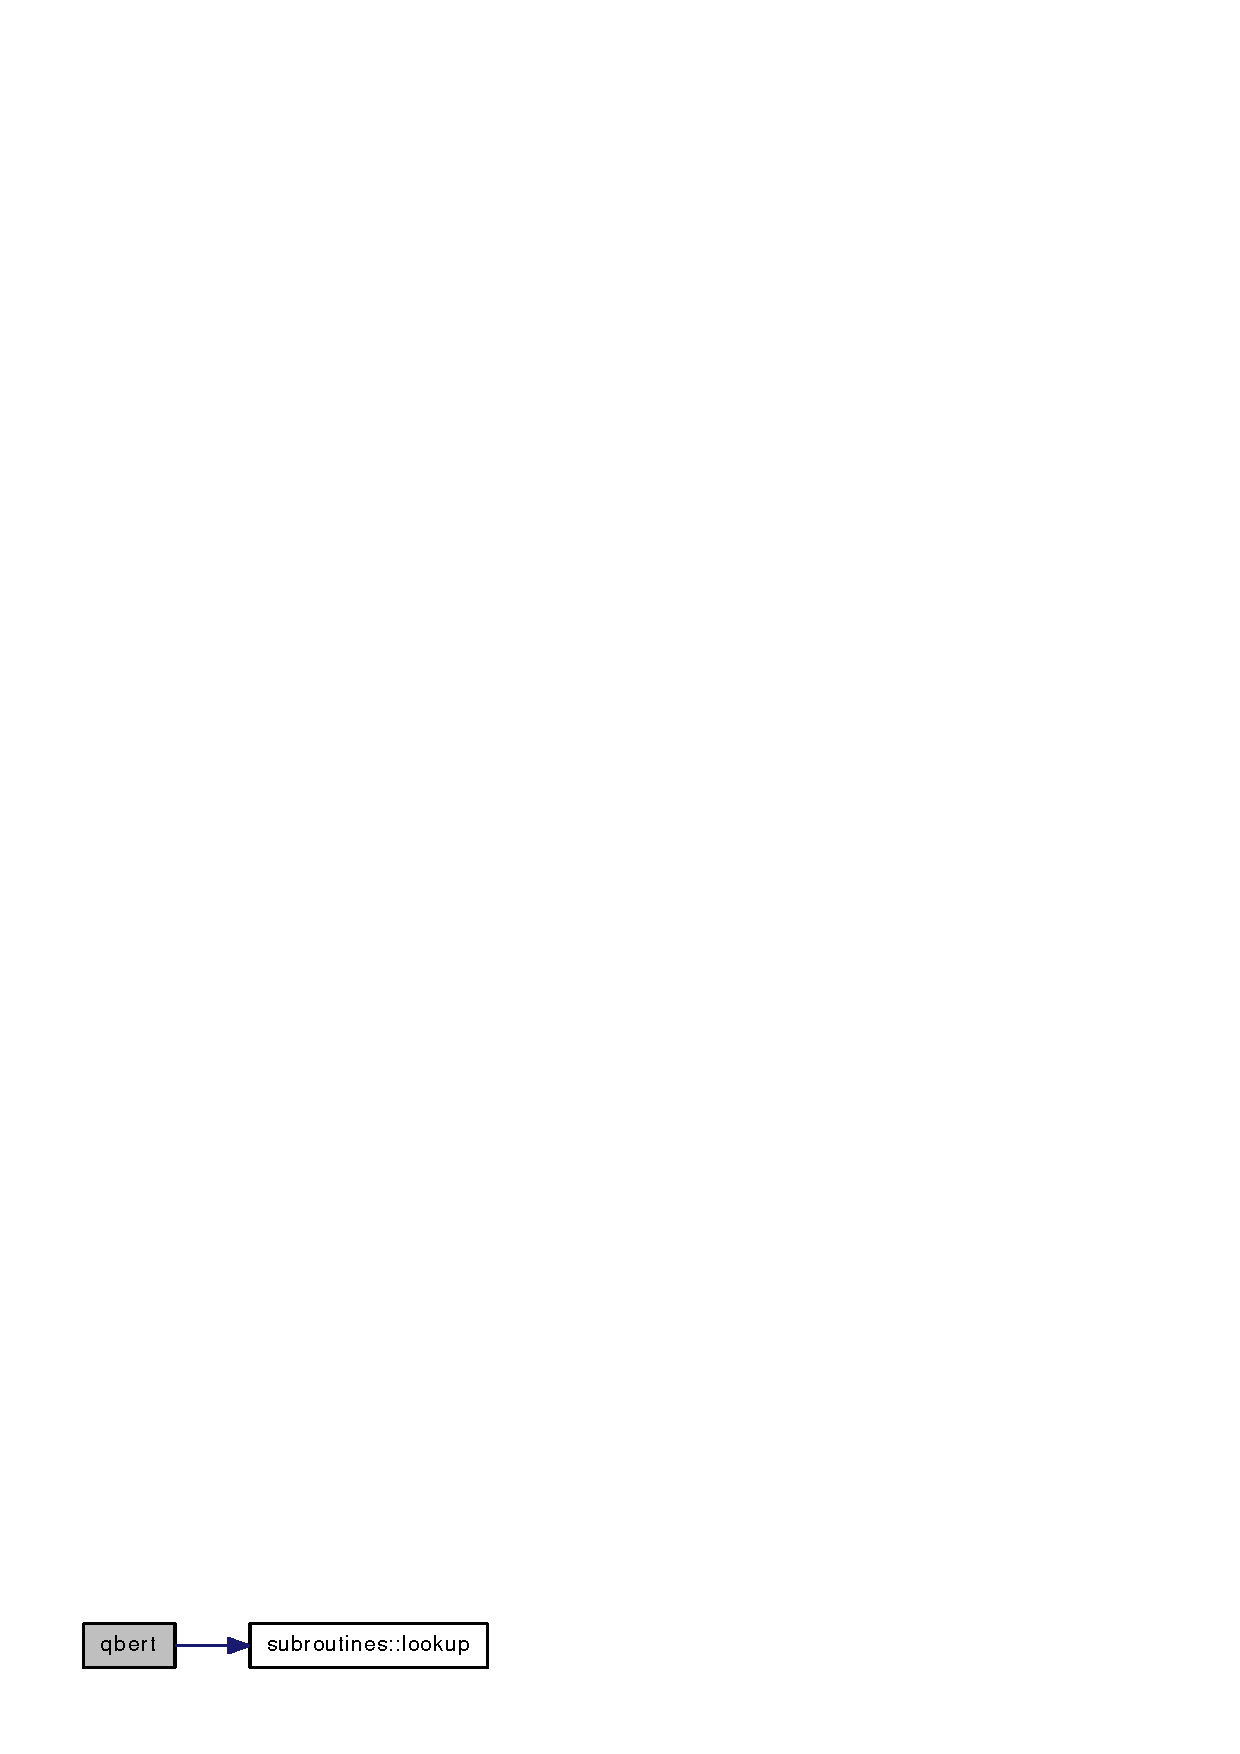
\includegraphics[width=119pt]{qbert_8f90_a5a21baca5ea0faeed24450fd8c0b5e3a_cgraph}
\end{center}
\end{figure}
\hypertarget{qbert_8f90_ab12dfa912fdebdcca6d6a613155662f6}{
\index{qbert.f90@{qbert.f90}!sort\_\-energies@{sort\_\-energies}}
\index{sort\_\-energies@{sort\_\-energies}!qbert.f90@{qbert.f90}}
\subsubsection[{sort\_\-energies}]{\setlength{\rightskip}{0pt plus 5cm}subroutine sort\_\-energies (INTEGER,dimension(3),intent(inout) {\em prods}, \/  REAL,intent(in) {\em A\_\-en}, \/  REAL,intent(in) {\em B\_\-en}, \/  REAL,intent(in) {\em C\_\-en})}}
\label{qbert_8f90_ab12dfa912fdebdcca6d6a613155662f6}


Definition at line 155 of file qbert.f90.
\hypertarget{readinput_8f90}{
\section{readinput.f90 File Reference}
\label{readinput_8f90}\index{readinput.f90@{readinput.f90}}
}
\subsection*{Modules}
\begin{DoxyCompactItemize}
\item 
module \hyperlink{namespacereadinput}{readinput}
\end{DoxyCompactItemize}
\subsection*{Functions/Subroutines}
\begin{DoxyCompactItemize}
\item 
subroutine \hyperlink{namespacereadinput_a29790780c02003cbcba39bb214e7ffd0}{readinput::buildnetwork} ()
\end{DoxyCompactItemize}

\hypertarget{sigma__test_8f90}{
\section{sigma\_\-test.f90 File Reference}
\label{sigma__test_8f90}\index{sigma\_\-test.f90@{sigma\_\-test.f90}}
}
\subsection*{Functions/Subroutines}
\begin{DoxyCompactItemize}
\item 
program \hyperlink{sigma__test_8f90_a5c784af74ebfdbe1d48bb07a07a2452f}{sigma\_\-test}
\end{DoxyCompactItemize}


\subsection{Function Documentation}
\hypertarget{sigma__test_8f90_a5c784af74ebfdbe1d48bb07a07a2452f}{
\index{sigma\_\-test.f90@{sigma\_\-test.f90}!sigma\_\-test@{sigma\_\-test}}
\index{sigma\_\-test@{sigma\_\-test}!sigma_test.f90@{sigma\_\-test.f90}}
\subsubsection[{sigma\_\-test}]{\setlength{\rightskip}{0pt plus 5cm}program sigma\_\-test ()}}
\label{sigma__test_8f90_a5c784af74ebfdbe1d48bb07a07a2452f}


Definition at line 1 of file sigma\_\-test.f90.

References parameters::EINIT, subroutines::esigma\_\-suite(), specdata::o2\_\-p\_\-ex, specdata::o2\_\-p\_\-ion, specdata::o3\_\-p\_\-ex, specdata::o3\_\-p\_\-ion, specdata::o\_\-p\_\-ex, specdata::o\_\-p\_\-ion, subroutines::psigma\_\-suite(), and subroutines::se\_\-info\_\-init().

Here is the call graph for this function:\nopagebreak
\begin{figure}[H]
\begin{center}
\leavevmode
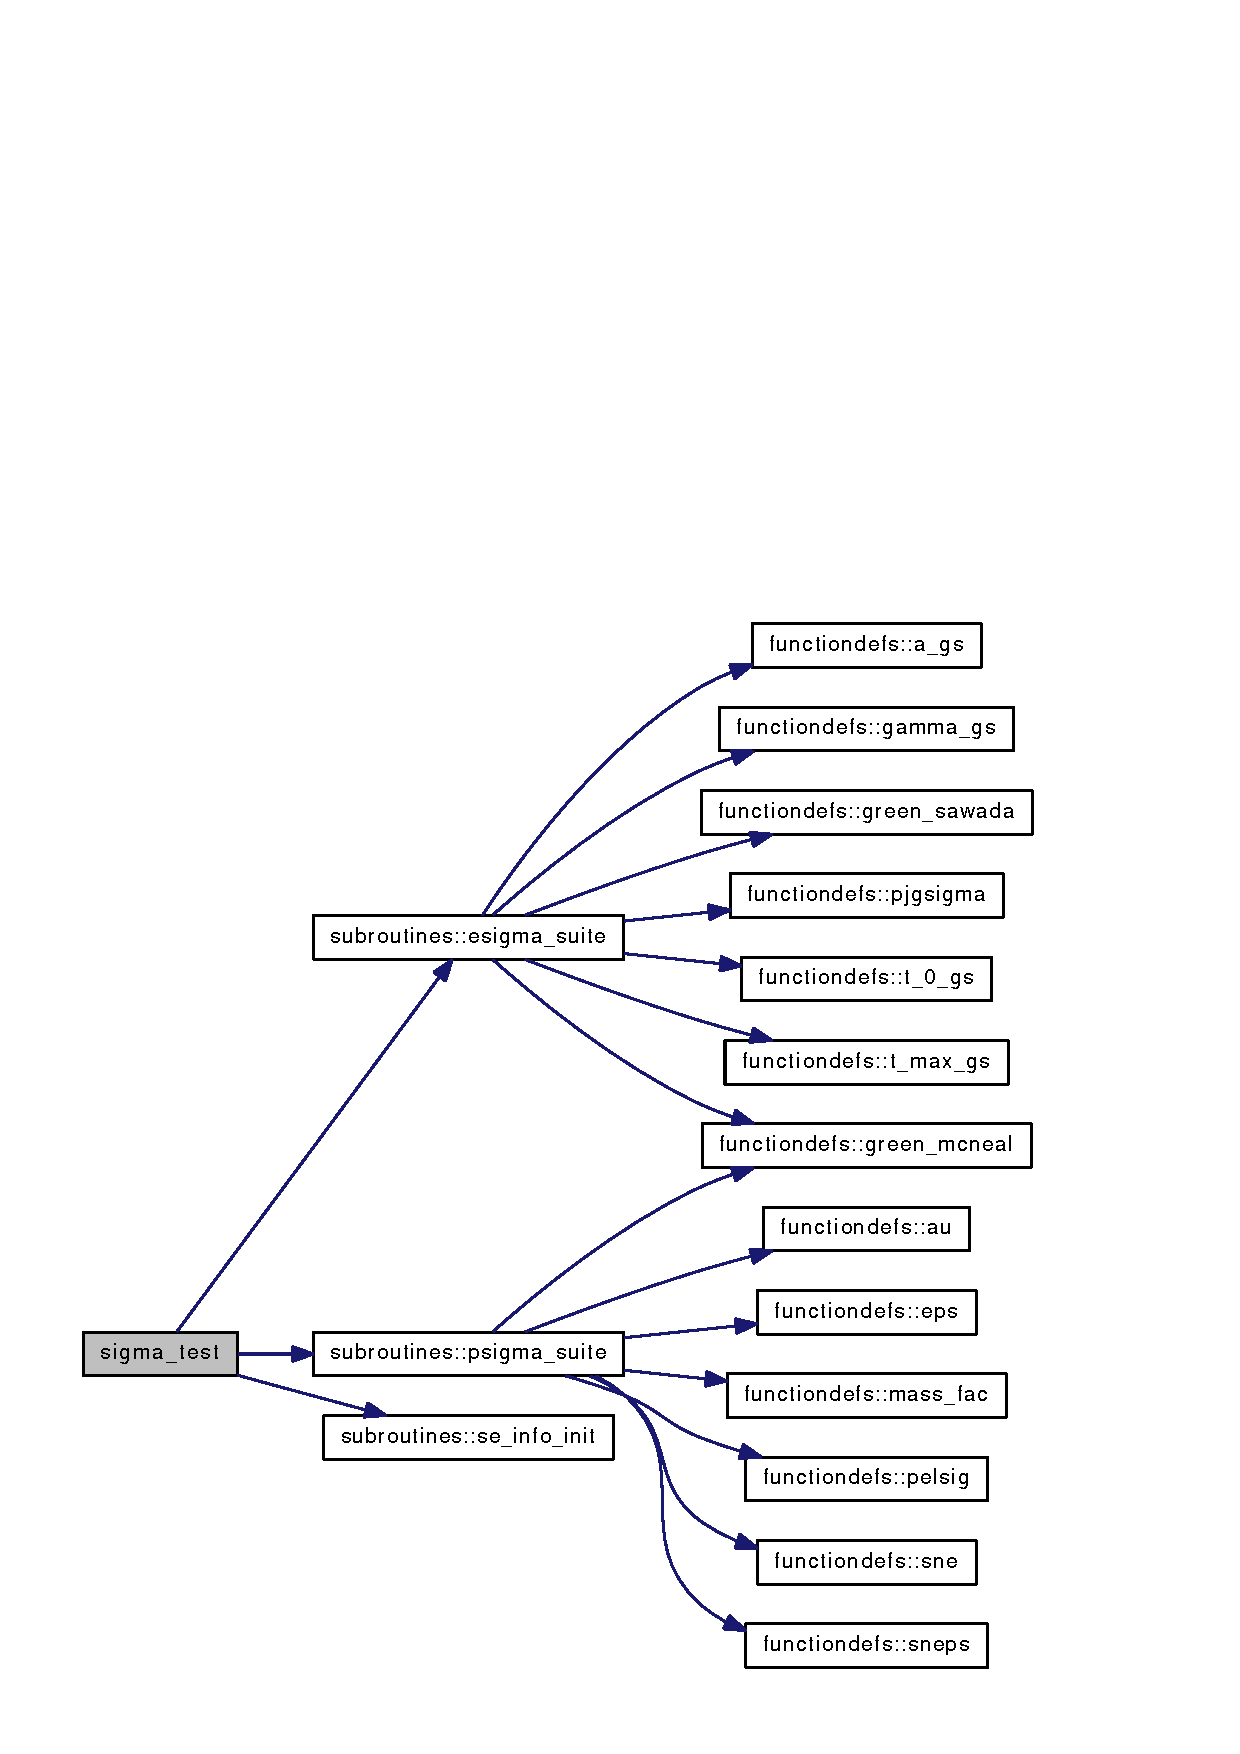
\includegraphics[width=250pt]{sigma__test_8f90_a5c784af74ebfdbe1d48bb07a07a2452f_cgraph}
\end{center}
\end{figure}

\hypertarget{specdata_8f90}{
\section{specdata.f90 File Reference}
\label{specdata_8f90}\index{specdata.f90@{specdata.f90}}
}
\subsection*{Modules}
\begin{DoxyCompactItemize}
\item 
module \hyperlink{namespacespecdata}{specdata}
\end{DoxyCompactItemize}
\subsection*{Variables}
\begin{DoxyCompactItemize}
\item 
TYPE(EPG\_\-EXSTATE), dimension(5), parameter \hyperlink{namespacespecdata_ae681c0bc4ab2fa5470a5956b4bec78d0}{specdata::o2\_\-p\_\-ex} = (/ EPG\_\-EXSTATE( ,0.092,2.50,0.5,3.0 ,0.98), EPG\_\-EXSTATE(,0.109,4.19,0.5,3.0 ,1.64), EPG\_\-EXSTATE(,0.57 ,17.6,0.5,0.9 ,4.5) , EPG\_\-EXSTATE(,4.73 ,51.7,0.5,0.75,8.4) , EPG\_\-EXSTATE( ,0.83 ,80.7,0.5,0.85,9.9) /)
\item 
TYPE(EPG\_\-EXSTATE), dimension(4), parameter \hyperlink{namespacespecdata_ae83fc5fae3d6873e5453849a6289952f}{specdata::o\_\-p\_\-ex} = (/ EPG\_\-EXSTATE(,0.51 ,5.4 ,1.0,1.0,1.85), EPG\_\-EXSTATE(,0.075,8.7 ,1.0,1.0,4.18), EPG\_\-EXSTATE(,0.38 ,37.2,1.0,1.0,9.53), EPG\_\-EXSTATE(,0.55 ,16.1,1.0,1.0,9.20) /)
\item 
TYPE(EPG\_\-EXSTATE), dimension(1), parameter \hyperlink{namespacespecdata_a5715afaf9a7cd31ff6c899aec265dc7e}{specdata::o3\_\-p\_\-ex} = (/ EPG\_\-EXSTATE(, 1.0, 20.00, 1.0, 2.5, 4.9) /)
\item 
TYPE(EPG\_\-IONSTATE), dimension(7), parameter \hyperlink{namespacespecdata_a1de88d1ad1d0aa421deaf2c5ac887ed8}{specdata::o2\_\-p\_\-ion} = (/ EPG\_\-IONSTATE(,9.56D0,45.8,0.61D0,1.26D0,12.1D0) , EPG\_\-IONSTATE(,5.38D0,127.1,1.1D0,0.58D0,16.1D0) , EPG\_\-IONSTATE(,5.25D0,170.3,1.1D0,0.60D0,16.9D0) , EPG\_\-IONSTATE(,3.19D0,142.4,1.1D0,0.58D0,18.2D0), EPG\_\-IONSTATE(,0.94D0,140.8,1.1D0,0.58D0,23.0D0) , EPG\_\-IONSTATE(,15.6D0,56.0,1.2D0,0.72D0,18.0D0) , EPG\_\-IONSTATE(,8.75D0,57.0,1.2D0,0.72D0,22.0D0) /)
\item 
TYPE(EPG\_\-IONSTATE), dimension(3), parameter \hyperlink{namespacespecdata_a67659f2839588aff464762d181bccdd7}{specdata::o\_\-p\_\-ion} = (/ EPG\_\-IONSTATE(,20.4,61.5,0.82,0.75,13.6), EPG\_\-IONSTATE(,25.4,69.5,0.82,0.75,16.9), EPG\_\-IONSTATE(,10.8,72.8,0.82,0.75,18.5) /)
\item 
TYPE(EPG\_\-IONSTATE), dimension(1), parameter \hyperlink{namespacespecdata_a42d18c80256a5ca2ccebe8a3f4d451a0}{specdata::o3\_\-p\_\-ion} = (/ EPG\_\-IONSTATE(, 40.00, 105.00, 1.00, 0.75, 12.43 ) /)
\item 
TYPE(ALWD\_\-EXSTATE), dimension(2), parameter \hyperlink{namespacespecdata_accca75874b57e169b91c0b680bffd51f}{specdata::o2\_\-e\_\-ex\_\-alwd} = (/ ALWD\_\-EXSTATE(,8.4,0.254,0.037,1.19,2.31), ALWD\_\-EXSTATE(,9.9,0.0285,0.622,1.38,3.44) /)
\item 
TYPE(FBDN\_\-EXSTATE), dimension(3), parameter \hyperlink{namespacespecdata_af2d6b8fc566715d79d76b79cc900229e}{specdata::o2\_\-e\_\-ex\_\-fbdn} = (/ FBDN\_\-EXSTATE(,1.64,0.0005,3.0,3.0,1.0) , FBDN\_\-EXSTATE(,0.98,0.0005,3.0,3.0,1.0) , FBDN\_\-EXSTATE(,4.5,0.021,0.9,1.0,1.0) /)
\item 
TYPE(ALWD\_\-EXSTATE), dimension(2), parameter \hyperlink{namespacespecdata_ac6de9abf8a4350031cdeed967f2b21b6}{specdata::o\_\-e\_\-ex\_\-alwd} = (/ ALWD\_\-EXSTATE(,9.53,0.0560,0.320,0.86,1.440), ALWD\_\-EXSTATE(,12.10,0.0310,0.610,1.26,0.490) /)
\item 
TYPE(FBDN\_\-EXSTATE), dimension(2), parameter \hyperlink{namespacespecdata_a31f902ca9efd2ca7817a66af34743c3d}{specdata::o\_\-e\_\-ex\_\-fbdn} = (/ FBDN\_\-EXSTATE(,1.85,0.0100,1.000,1.00,2.00) , FBDN\_\-EXSTATE(,4.18,0.0042,1.00,0.50,1.000) /)
\item 
TYPE(IONSTATE), dimension(1), parameter \hyperlink{namespacespecdata_a7040a4bcf92d1e17f6158536ca8d5b0a}{specdata::o2\_\-e\_\-ion} = (/ IONSTATE(,12.1,0.475,0.0,3.760,0.0,0.0,18.50,12.10,1.860,1000.0,24.20) /)
\item 
TYPE(IONSTATE), dimension(1), parameter \hyperlink{namespacespecdata_aa92d120444752fc22443b31d087da308}{specdata::o\_\-e\_\-ion} = (/ IONSTATE(,13.6,1.03,0.0,1.81,0.0,0.0,13.0,-\/0.815,6.41,3450.0,162.0) /)
\end{DoxyCompactItemize}

\hypertarget{subroutines_8f90}{
\section{subroutines.f90 File Reference}
\label{subroutines_8f90}\index{subroutines.f90@{subroutines.f90}}
}
\subsection*{Modules}
\begin{DoxyCompactItemize}
\item 
module \hyperlink{namespacesubroutines}{subroutines}
\end{DoxyCompactItemize}
\subsection*{Functions/Subroutines}
\begin{DoxyCompactItemize}
\item 
subroutine \hyperlink{namespacesubroutines_a27505ee5071c93bb5f1e570995a1ac42}{subroutines::lookup} (name, node, id, atoms, charge)
\item 
subroutine \hyperlink{namespacesubroutines_a0ce9ee9331d3c0bba11e3e00fbd7e07b}{subroutines::writereactions} (node)
\item 
subroutine \hyperlink{namespacesubroutines_ad97e0b9db9cfe6329f9f8fdb886077e7}{subroutines::hopping} (i\_\-in, j\_\-in, k\_\-in, i\_\-out, j\_\-out, k\_\-out, prob)
\item 
subroutine \hyperlink{namespacesubroutines_a7a31d5c9fbda24651c932b0466618567}{subroutines::fallout} (root, temp, prevNode, nextNode)
\item 
subroutine \hyperlink{namespacesubroutines_af4c69699bd3e0e4aa05607a7e94044dc}{subroutines::find\_\-empty\_\-site} (in\_\-coords, out\_\-coords, null)
\item 
subroutine \hyperlink{namespacesubroutines_ac847bd99eab89bdc881d885b2808624d}{subroutines::wait\_\-calc} (temp)
\item 
subroutine \hyperlink{namespacesubroutines_af250b65cb2805243dd52e4e3535f4c5a}{subroutines::counter} ()
\item 
subroutine \hyperlink{namespacesubroutines_a0a51843cbd2415487f29e4314e1de97a}{subroutines::transport} (prev, curr, next)
\item 
subroutine \hyperlink{namespacesubroutines_a37b9d3b519b164f5ef3835bf4e1e4f8c}{subroutines::psigma\_\-suite} (energy, psigmas, psigij, psigexj, o\_\-psigmas, o\_\-psigij, o\_\-psigexj, o3\_\-psigmas, o3\_\-psigij, o3\_\-psigexj)
\item 
subroutine \hyperlink{namespacesubroutines_a27620c6392f4cd49238c295cbe60e179}{subroutines::esigma\_\-suite} (se\_\-box)
\item 
subroutine \hyperlink{namespacesubroutines_a3185cd857374fa3b0a19f2a56e6474df}{subroutines::p\_\-ion\_\-select} (psigij, e\_\-ion, e\_\-se, thinghit)
\item 
subroutine \hyperlink{namespacesubroutines_acad706394e0b01bbd1e5345585dace59}{subroutines::p\_\-ex\_\-select} (psigexj, e\_\-exc, thinghit)
\item 
subroutine \hyperlink{namespacesubroutines_acad777e3f27acb4f7e0f7b35035ae54a}{subroutines::e\_\-ion\_\-select} (se\_\-box, e\_\-ion, e\_\-se, null, thinghit)
\item 
subroutine \hyperlink{namespacesubroutines_a0f09eb60b63730612ddd7801066ce49b}{subroutines::e\_\-ex\_\-select} (se\_\-box, e\_\-exc, null, thinghit)
\item 
subroutine \hyperlink{namespacesubroutines_a10f3c575d44eedaf9b0a95ed9a64e3ab}{subroutines::elastic\_\-event} (energy, e\_\-loss, labtheta)
\item 
subroutine \hyperlink{namespacesubroutines_aece587c9d144811189bd1ccf8a59f189}{subroutines::se\_\-info\_\-init} (se\_\-box)
\item 
subroutine \hyperlink{namespacesubroutines_a1d1775ee81394d8c078c760678a530e2}{subroutines::se\_\-info\_\-garbage} (se\_\-box)
\item 
subroutine \hyperlink{namespacesubroutines_a4d9b1fbbdcfc2b420201a7ca71c4e782}{subroutines::init\_\-node} (root, temp\_\-node, x, y, z)
\item 
subroutine \hyperlink{namespacesubroutines_a7580fc0416f20d44b3cfa79ebc20a839}{subroutines::wipe\_\-node} (x, y, z)
\item 
subroutine \hyperlink{namespacesubroutines_a5f9a688681311ebc691561ec51015d0f}{subroutines::new\_\-reaction} (i, j, k, root, temp, prevNode, nextNode, error)
\item 
subroutine \hyperlink{namespacesubroutines_ae942148085820c335aea6798ad4e7e7e}{subroutines::new\_\-electron} (se\_\-box, root, temp, prevNode, nextNode)
\item 
subroutine \hyperlink{namespacesubroutines_aae3cb4fad8f95b0869777449a6bc496f}{subroutines::analyzereaction} (reactnode, speciesnum, yield, nature)
\item 
subroutine \hyperlink{namespacesubroutines_abbce0f7ec92c43ac91db25f512531642}{subroutines::trackwrite} (coords, energy, e\_\-branch, electron)
\end{DoxyCompactItemize}

\hypertarget{typedefs_8f90}{
\section{typedefs.f90 File Reference}
\label{typedefs_8f90}\index{typedefs.f90@{typedefs.f90}}
}
\subsection*{Data Types}
\begin{DoxyCompactItemize}
\item 
type \hyperlink{typetypedefs_1_1wait__info}{typedefs::wait\_\-info}
\item 
type \hyperlink{typetypedefs_1_1rate__info}{typedefs::rate\_\-info}
\item 
type \hyperlink{typetypedefs_1_1sigma__box}{typedefs::sigma\_\-box}
\item 
type \hyperlink{typetypedefs_1_1ionstate}{typedefs::ionstate}
\item 
type \hyperlink{typetypedefs_1_1alwd__exstate}{typedefs::alwd\_\-exstate}
\item 
type \hyperlink{typetypedefs_1_1fbdn__exstate}{typedefs::fbdn\_\-exstate}
\item 
type \hyperlink{typetypedefs_1_1epg__exstate}{typedefs::epg\_\-exstate}
\item 
type \hyperlink{typetypedefs_1_1epg__ionstate}{typedefs::epg\_\-ionstate}
\item 
type \hyperlink{typetypedefs_1_1se__info}{typedefs::se\_\-info}
\item 
type \hyperlink{typetypedefs_1_1node}{typedefs::node}
\item 
type \hyperlink{typetypedefs_1_1species}{typedefs::species}
\item 
type \hyperlink{typetypedefs_1_1reaction}{typedefs::reaction}
\item 
type \hyperlink{typetypedefs_1_1reaction__info}{typedefs::reaction\_\-info}
\end{DoxyCompactItemize}
\subsection*{Modules}
\begin{DoxyCompactItemize}
\item 
module \hyperlink{namespacetypedefs}{typedefs}
\end{DoxyCompactItemize}

\printindex
\end{document}
